% Options for packages loaded elsewhere
\PassOptionsToPackage{unicode}{hyperref}
\PassOptionsToPackage{hyphens}{url}
%
\documentclass[
]{book}
\usepackage{amsmath,amssymb}
\usepackage{iftex}
\ifPDFTeX
  \usepackage[T1]{fontenc}
  \usepackage[utf8]{inputenc}
  \usepackage{textcomp} % provide euro and other symbols
\else % if luatex or xetex
  \usepackage{unicode-math} % this also loads fontspec
  \defaultfontfeatures{Scale=MatchLowercase}
  \defaultfontfeatures[\rmfamily]{Ligatures=TeX,Scale=1}
\fi
\usepackage{lmodern}
\ifPDFTeX\else
  % xetex/luatex font selection
\fi
% Use upquote if available, for straight quotes in verbatim environments
\IfFileExists{upquote.sty}{\usepackage{upquote}}{}
\IfFileExists{microtype.sty}{% use microtype if available
  \usepackage[]{microtype}
  \UseMicrotypeSet[protrusion]{basicmath} % disable protrusion for tt fonts
}{}
\makeatletter
\@ifundefined{KOMAClassName}{% if non-KOMA class
  \IfFileExists{parskip.sty}{%
    \usepackage{parskip}
  }{% else
    \setlength{\parindent}{0pt}
    \setlength{\parskip}{6pt plus 2pt minus 1pt}}
}{% if KOMA class
  \KOMAoptions{parskip=half}}
\makeatother
\usepackage{xcolor}
\usepackage{color}
\usepackage{fancyvrb}
\newcommand{\VerbBar}{|}
\newcommand{\VERB}{\Verb[commandchars=\\\{\}]}
\DefineVerbatimEnvironment{Highlighting}{Verbatim}{commandchars=\\\{\}}
% Add ',fontsize=\small' for more characters per line
\usepackage{framed}
\definecolor{shadecolor}{RGB}{248,248,248}
\newenvironment{Shaded}{\begin{snugshade}}{\end{snugshade}}
\newcommand{\AlertTok}[1]{\textcolor[rgb]{0.94,0.16,0.16}{#1}}
\newcommand{\AnnotationTok}[1]{\textcolor[rgb]{0.56,0.35,0.01}{\textbf{\textit{#1}}}}
\newcommand{\AttributeTok}[1]{\textcolor[rgb]{0.13,0.29,0.53}{#1}}
\newcommand{\BaseNTok}[1]{\textcolor[rgb]{0.00,0.00,0.81}{#1}}
\newcommand{\BuiltInTok}[1]{#1}
\newcommand{\CharTok}[1]{\textcolor[rgb]{0.31,0.60,0.02}{#1}}
\newcommand{\CommentTok}[1]{\textcolor[rgb]{0.56,0.35,0.01}{\textit{#1}}}
\newcommand{\CommentVarTok}[1]{\textcolor[rgb]{0.56,0.35,0.01}{\textbf{\textit{#1}}}}
\newcommand{\ConstantTok}[1]{\textcolor[rgb]{0.56,0.35,0.01}{#1}}
\newcommand{\ControlFlowTok}[1]{\textcolor[rgb]{0.13,0.29,0.53}{\textbf{#1}}}
\newcommand{\DataTypeTok}[1]{\textcolor[rgb]{0.13,0.29,0.53}{#1}}
\newcommand{\DecValTok}[1]{\textcolor[rgb]{0.00,0.00,0.81}{#1}}
\newcommand{\DocumentationTok}[1]{\textcolor[rgb]{0.56,0.35,0.01}{\textbf{\textit{#1}}}}
\newcommand{\ErrorTok}[1]{\textcolor[rgb]{0.64,0.00,0.00}{\textbf{#1}}}
\newcommand{\ExtensionTok}[1]{#1}
\newcommand{\FloatTok}[1]{\textcolor[rgb]{0.00,0.00,0.81}{#1}}
\newcommand{\FunctionTok}[1]{\textcolor[rgb]{0.13,0.29,0.53}{\textbf{#1}}}
\newcommand{\ImportTok}[1]{#1}
\newcommand{\InformationTok}[1]{\textcolor[rgb]{0.56,0.35,0.01}{\textbf{\textit{#1}}}}
\newcommand{\KeywordTok}[1]{\textcolor[rgb]{0.13,0.29,0.53}{\textbf{#1}}}
\newcommand{\NormalTok}[1]{#1}
\newcommand{\OperatorTok}[1]{\textcolor[rgb]{0.81,0.36,0.00}{\textbf{#1}}}
\newcommand{\OtherTok}[1]{\textcolor[rgb]{0.56,0.35,0.01}{#1}}
\newcommand{\PreprocessorTok}[1]{\textcolor[rgb]{0.56,0.35,0.01}{\textit{#1}}}
\newcommand{\RegionMarkerTok}[1]{#1}
\newcommand{\SpecialCharTok}[1]{\textcolor[rgb]{0.81,0.36,0.00}{\textbf{#1}}}
\newcommand{\SpecialStringTok}[1]{\textcolor[rgb]{0.31,0.60,0.02}{#1}}
\newcommand{\StringTok}[1]{\textcolor[rgb]{0.31,0.60,0.02}{#1}}
\newcommand{\VariableTok}[1]{\textcolor[rgb]{0.00,0.00,0.00}{#1}}
\newcommand{\VerbatimStringTok}[1]{\textcolor[rgb]{0.31,0.60,0.02}{#1}}
\newcommand{\WarningTok}[1]{\textcolor[rgb]{0.56,0.35,0.01}{\textbf{\textit{#1}}}}
\usepackage{longtable,booktabs,array}
\usepackage{calc} % for calculating minipage widths
% Correct order of tables after \paragraph or \subparagraph
\usepackage{etoolbox}
\makeatletter
\patchcmd\longtable{\par}{\if@noskipsec\mbox{}\fi\par}{}{}
\makeatother
% Allow footnotes in longtable head/foot
\IfFileExists{footnotehyper.sty}{\usepackage{footnotehyper}}{\usepackage{footnote}}
\makesavenoteenv{longtable}
\usepackage{graphicx}
\makeatletter
\def\maxwidth{\ifdim\Gin@nat@width>\linewidth\linewidth\else\Gin@nat@width\fi}
\def\maxheight{\ifdim\Gin@nat@height>\textheight\textheight\else\Gin@nat@height\fi}
\makeatother
% Scale images if necessary, so that they will not overflow the page
% margins by default, and it is still possible to overwrite the defaults
% using explicit options in \includegraphics[width, height, ...]{}
\setkeys{Gin}{width=\maxwidth,height=\maxheight,keepaspectratio}
% Set default figure placement to htbp
\makeatletter
\def\fps@figure{htbp}
\makeatother
\setlength{\emergencystretch}{3em} % prevent overfull lines
\providecommand{\tightlist}{%
  \setlength{\itemsep}{0pt}\setlength{\parskip}{0pt}}
\setcounter{secnumdepth}{5}
\usepackage{booktabs}
\usepackage{lscape}

\ifLuaTeX
  \usepackage{selnolig}  % disable illegal ligatures
\fi
\usepackage[]{natbib}
\bibliographystyle{apalike}
\IfFileExists{bookmark.sty}{\usepackage{bookmark}}{\usepackage{hyperref}}
\IfFileExists{xurl.sty}{\usepackage{xurl}}{} % add URL line breaks if available
\urlstyle{same}
\hypersetup{
  pdftitle={Metode Numerik Menggunakan R Untuk Teknik Lingkungan},
  pdfauthor={Mohammad Rosidi},
  hidelinks,
  pdfcreator={LaTeX via pandoc}}

\title{Metode Numerik Menggunakan R Untuk Teknik Lingkungan}
\author{Mohammad Rosidi}
\date{2023-08-10}

\usepackage{amsthm}
\newtheorem{theorem}{Teorema}[chapter]
\newtheorem{lemma}{Lemma}[chapter]
\newtheorem{corollary}{Corollary}[chapter]
\newtheorem{proposition}{Proposition}[chapter]
\newtheorem{conjecture}{Conjecture}[chapter]
\theoremstyle{definition}
\newtheorem{definition}{Definition}[chapter]
\theoremstyle{definition}
\newtheorem{example}{Contoh}[chapter]
\theoremstyle{definition}
\newtheorem{exercise}{Exercise}[chapter]
\theoremstyle{definition}
\newtheorem{hypothesis}{Hypothesis}[chapter]
\theoremstyle{remark}
\newtheorem*{remark}{Remark}
\newtheorem*{solution}{Solution}
\begin{document}
\maketitle

{
\setcounter{tocdepth}{1}
\tableofcontents
}
\hypertarget{pengantar}{%
\chapter*{Pengantar}\label{pengantar}}
\addcontentsline{toc}{chapter}{Pengantar}

Metone Numerik Menggunakan R Untuk Teknik Lingkungan merupakan buku yang penulis tulis dengan harapan dapat menjadi salah satu rujukan mahasiswa khusunya Teknik Lingkungan yang tertarik untuk belajar \texttt{R}. Selain itu, buku ini merupakan salah satu cara pengabdian penulis guna menyediakan sumber pembelajaran yang bersifat terbuka dan dapat diakses seluruh kalangan secara gratis.

\textbf{Mengapa perlu menulis buku ini?} Penulis merasa selama ini buku-buku metode numerik yang ada di pasaran masih didominasi oleh buku-buku pemrograman berbasis Matlab. Atas dasar tersebut, penulis merasa perlu adanya alternatif pembelajaran menggunakan bahasa pemrograman lain.

\textbf{Mengapa harus \texttt{R}?} Sejak lama \texttt{R} dikenal secara luas sebagai bahasa pemrograman yang digunakan dalam bidang statistika dan \emph{data science}. Selain kedua hal tersebut, \texttt{R} menyediakan basis dalam melakukan komputasi numerik yang dapat digunakan untuk menyusun sebuah program atau paket yang dapat menyelesaikan persoalan-persoalan metode numerik. Saat ini telah banyak paket yang dikembangkan khusus untuk menangani penyelesaian persamaan matematika menggunakan metode numerik. Paket-paket yang penulis maksud dan penulis sertakan dalam buku ini, antara lain: \texttt{limSolve}, \texttt{gaussquad}, \texttt{pracma}, \texttt{orthopolynom}, \texttt{deSolve}, \texttt{ReacTran}, dll.

\textbf{Apakah saya harus fasih \texttt{R} untuk dapat menggunakan buku ini?} tidak. Buku ini telah disusun sedemikian rupa sehingga pemula sekalipun dapat dengan mudah belajar dasar-dasar pemrograman \texttt{R}.

\textbf{Apa saja yang tersedia dalam buku ini?} Pada buku ini telah penulis sediakan beberapa hal, antara lain:

\begin{itemize}
\tightlist
\item
  teori dasar metode numerik
\item
  algoritma penyelesaian menggunakan metode numerik
\item
  fungsi dan cara iterasi dalam menyelesaikan suatu persamaan menggunakan metode numerik
\item
  studi kasus dalam bidang Teknik Lingkungan, dan
\item
  latihan soal
\end{itemize}

\hypertarget{gambaran-isi-buku}{%
\section*{Gambaran Isi Buku}\label{gambaran-isi-buku}}
\addcontentsline{toc}{section}{Gambaran Isi Buku}

Buku ini disusun ke dalam 11 \textbf{Chapter}. Secara garis besar gambaran ke-11 \textbf{Chapter} tersebut antara lain:

\textbf{Dasar pemrograman menggunakan \texttt{R}}

\begin{itemize}
\tightlist
\item
  \textbf{Chapter 1} : pada chapter ini dibahas sejarah, fitur dan karakteristik bahasa \texttt{R}, dan cara berinteraksi dengan \texttt{R} melalui \texttt{Rstudio}.
\item
  \textbf{Chapter 2} : pada chapter ini dibahas terkait cara melakukan perhitungan atau kalkulasi matematis menggunakan \texttt{R}. Selain itu, pada chapter ini juga dibahas terkait operator-operator yang digunakan dalam \texttt{R}, jenis data pada \texttt{R}, dan bagaimana cara menyimpan nilai ke dalam variabel.
\item
  \textbf{chapter 3} : chapter ini membahas cara membuat sebuah visualisasi data dan cara mengatur parameter visualisasi data pada \texttt{R}.
\item
  \textbf{chapter 4} : chapter ini membahas cara membentuk sebuah fungsi dan cara melakukan iterasi pada \texttt{R}.
\end{itemize}

\textbf{Metode Numerik Menggunakan \texttt{R}}

Pada bagian ini pembaca akan belajar teori dan aplikasi metode numerik menggunakan \texttt{R}. Adapun hal-hal yang dibahas dalam bagian ini antara lain:

\begin{itemize}
\tightlist
\item
  pengantar metode numerik (\textbf{chapter 5})
\item
  aljabar linier (\textbf{chapter 6})
\item
  akar persamaan non-linier (\textbf{chapter 7})
\item
  interpolasi dan ekstrapolasi (\textbf{chapter 8})
\item
  diferensiasi dan integrasi numerik (\textbf{chapter 9})
\item
  persamaan diferensial (\textbf{chapter 10})
\end{itemize}

\textbf{Analisis dan pemodelan statistik}

Pada bagian ini pembaca akan belajar bagaimana cara membaca data menggunakan \texttt{R} dan cara melakukan analisis data menggunakan \texttt{R} (\textbf{chapter 11}). Pada bagian lainnya pembaca akan belajar cara membentuk sebuah model regresi linier dan logistik pada \texttt{R} (\textbf{chapter 12})

\hypertarget{cara-berkontribusi-dalam-buku-ini}{%
\section*{Cara Berkontribusi dalam Buku Ini}\label{cara-berkontribusi-dalam-buku-ini}}
\addcontentsline{toc}{section}{Cara Berkontribusi dalam Buku Ini}

Buku ini tidaklah sempurna. Masih terdapat banyak kekurangan dalam buku ini. Namun, kekurangan tersebut tetaplah dapat diperbaiki. Penulis membuka ruang seluas-luasnya dalam melakukan perbaikan dalam buku ini bagi pembaca. Untuk dapat melakukannya pembaca hanya perlu melakukan \emph{pull request} ke akun github penulis atau pembaca dapat melakukannya melalui email yang selanjutnya akan penulis jadikan acuan perbaikan.

Github : \url{https://github.com/mohrosidi/metode_numerik}
Email : \href{mailto:moh.rosidi2610@gmail.com}{\nolinkurl{moh.rosidi2610@gmail.com}}

\hypertarget{ucapan-terima-kasih}{%
\section*{Ucapan Terima Kasih}\label{ucapan-terima-kasih}}
\addcontentsline{toc}{section}{Ucapan Terima Kasih}

Buku ini tidak akan ada apabila tidak adanya inspirasi dari rekan-rekan Teknik Lingkungan ITB dan paket \texttt{bookdown} dari Rstudio. Ucapan terima kasih juga penulis sampaikan komunitas \texttt{R} Idonesia yang telah memberikan banyak pelajaran bagi penulis dalam belajar \texttt{R}. Tidak pula penulis mengucapkan terima kasih pada pengembang paket-paket metode numerik yang karyanya telah membantu saya dalam menyusun buku ini.

\hypertarget{lisensi}{%
\section*{Lisensi}\label{lisensi}}
\addcontentsline{toc}{section}{Lisensi}

This
work is licensed under a
Creative
Commons Attribution-ShareAlike 4.0 International License.

\hypertarget{intro}{%
\chapter{Bahasa Pemrograman R}\label{intro}}

Dewasa ini tersedia banyak sekali \emph{software} yang dapat digunakan untuk membantu kita dalam melakukan analisa data. \emph{software} yang digunakan dapat berupa \emph{software} berbayar atau gratis.

\texttt{R} merupakan merupakan salah satu \emph{software} gratis yang sangat populer di Indonesia. Kemudahan penggunaan serta banyaknya besarnya dukungan komunitas membuat \texttt{R} menjadi salah satu bahasa pemrograman paling populer di dunia.

Paket yang disediakan untuk analisis statistika dan analisa numerik juga sangat lengkap dan terus bertambah setiap saat. Hal ini membuat \texttt{R} banyak digunakan oleh para analis data.

Pada \emph{chapter} ini penulis akan memperkenalkan kepada pembaca mengenai bahasa pemrograman \texttt{R}. Mulai dari sejarah, cara instalasi sampai dengan bagaimana kita memanfaatkan fitur dasar bantuan untuk menggali lebih jauh tentang fungsi-fungsi \texttt{R}

\hypertarget{sejarahR}{%
\section{Sejarah R}\label{sejarahR}}

\texttt{R} Merupakan bahasa yang digunakan dalam komputasi \textbf{statistik} yang pertama kali dikembangkan oleh \textbf{Ross Ihaka} dan \textbf{Robert Gentlement} di University of Auckland New Zealand yang merupakan akronim dari nama depan kedua pembuatnya. Sebelum \texttt{R} dikenal ada \texttt{S} yang dikembangkan oleh \textbf{John Chambers} dan rekan-rekan dari \textbf{Bell Laboratories} yang memiliki fungsi yang sama untuk komputasi statistik. Hal yang membedakan antara keduanya adalah \texttt{R} merupakan sistem komputasi yang bersifat gratis.Logo \texttt{R} dapat dilihat pada Gambar \ref{fig:Logo}.

\begin{figure}

{\centering 
\includegraphics[width=0.4\linewidth]{./images/r-icon} 

}

\caption{Logo R.}\label{fig:Logo}
\end{figure}

\texttt{R} dapat dibilang merupakan aplikasi sistem \textbf{statistik} yang kaya. Hal ini disebabkan banyak sekali Paket yang dikembangkan oleh pengembang dan komunitas untuk keperluan analisa statistik seperti \emph{linear regression}, \emph{clustering}, \emph{statistical test}, dll. Selain itu, \texttt{R} juga dapat ditambahkan Paket-Paket lain yang dapat meningkatkan fiturnya.

Sebagai sebuah bahasa pemrograman yang banyak digunakan untuk keperluan analisa data, \texttt{R} dapat dioperasikan pada berbagai sistem operasi pada komputer. Adapun sistem operasi yang didukung antara lain: \texttt{UNIX}, \texttt{Linux}, \texttt{Windows}, dan \texttt{MacOS}.

\hypertarget{fiturR}{%
\section{Fitur dan Karakteristik R}\label{fiturR}}

\texttt{R} memiliki karakteristik yang berbeda dengan bahasa pemrograman lain seperti \texttt{C++},\texttt{python}, dll. \texttt{R} memiliki aturan/sintaks yang berbeda dengan bahasa pemrograman yang lain yang membuatnya memiliki ciri khas tersendiri dibanding bahasa pemrograman yang lain.

Beberapa ciri dan fitur pada \texttt{R} antara lain:

\begin{enumerate}
\def\labelenumi{\arabic{enumi}.}
\tightlist
\item
  \textbf{Bahasa \texttt{R} bersifat case sensitif}. maksudnya adalah dalam proses input \texttt{R} huruf besar dan kecil sangat diperhatikan. Sebagai contoh kita ingin melihat apakah objek A dan B pada sintaks berikut:
\end{enumerate}

\begin{Shaded}
\begin{Highlighting}[]
\NormalTok{A }\OtherTok{\textless{}{-}} \StringTok{"Andi"}
\NormalTok{B }\OtherTok{\textless{}{-}} \StringTok{"andi"}

\CommentTok{\# cek kedua objek A dan B}
\NormalTok{A }\SpecialCharTok{==}\NormalTok{ B}
\end{Highlighting}
\end{Shaded}

\begin{verbatim}
## [1] FALSE
\end{verbatim}

\begin{Shaded}
\begin{Highlighting}[]
\CommentTok{\# Kesimpulan : Kedua objek berbeda}
\end{Highlighting}
\end{Shaded}

\begin{enumerate}
\def\labelenumi{\arabic{enumi}.}
\setcounter{enumi}{1}
\tightlist
\item
  \textbf{Segala sesuatu yang ada pada program \texttt{R} akan diangap sebagai objek}. konsep objek ini sama dengan bahasa pemrograma berbasis objek yang lain seperti \texttt{Java}, \texttt{C++}, \texttt{python}, dll.Perbedaannya adalah bahasa \texttt{R} relatif lebih sederhana dibandingkan bahasa pemrograman berbasis obejk yang lain.
\item
  \textbf{interpreted language atau script}. Bahasa \texttt{R} memungkinkan pengguna untuk melakukan kerja pada \texttt{R} tanpa perlu kompilasi kode program menjadi bahasa mesin.
\item
  Mendukung proses \textbf{loop}, \textbf{decision making}, dan menyediakan berbagai jenis \textbf{operstor} (aritmatika, logika, dll).
\item
  \textbf{Mendukung export dan import berbagai format file}, seperti:TXT, CSV, XLS, dll.
\item
  \textbf{Mudah ditingkatkan melalui penambahan fungsi atau \emph{library}}. Penambahan Paket dapat dilakukan secara online melalui \href{https://cran.r-project.org/}{CRAN} atau melalui sumber seperti \href{https://github.com/}{github}.
\item
  \textbf{Menyedikan berbagai fungsi untuk keperluan visualisasi data}. Visualisasi data pada \texttt{R} dapat menggunakan Paket bawaan atau Paket lain seperti \texttt{ggplo2},\texttt{ggvis}, dll.
\end{enumerate}

\hypertarget{prosconsR}{%
\section{Kelebihan dan Kekurangan R}\label{prosconsR}}

Selain karena \texttt{R} dapat digunakan secara gratis terdapat \textbf{kelebihan} lain yang ditawarkan, antara lain:

\begin{enumerate}
\def\labelenumi{\arabic{enumi}.}
\tightlist
\item
  \textbf{Protability}. Penggunaan software dapat digunakan kapanpun tanpa terikat oleh masa berakhirnya lisensi.
\item
  \textbf{Multiplatform}. \texttt{R} bersifat \emph{Multiplatform Operating Systems}, dimana \emph{software} \texttt{R} lebih kompatibel dibanding \emph{software} statistika lainnya. Hal in berdampak pada kemudahan dalam penyesuaian jika pengguna harus berpindah sistem operasi karena \texttt{R} baik pada sistem operasi seperti \texttt{windows} akan sama pengoperasiannya dengan yang ada di \texttt{Linux} (Paket yang digunakan sama).
\item
  \textbf{General} dan \textbf{Cutting-edge}. Berbagai metode statistik baik metode klasik maupun baru telah diprogram kedalam \texttt{R}. Dengan demikian \emph{software} ini dapat digunakan untuk analisis statistika dengan pendekatan klasik dan pendekatan modern.
\item
  \textbf{Programable}. Pengguna dapat memprogram metode baru atau mengembangakan modifikasi dari analisis statistika yang telah ada pada sistem \texttt{R}.
\item
  \textbf{Berbasis analisis matriks}. Bahasa \texttt{R} sangat baik digunakan untuk \emph{programming} dengan basis matriks.
\item
  Fasiltas grafik yang lengkap.
\end{enumerate}

Adapun kekurangan dari \texttt{R} antara lain:

\begin{enumerate}
\def\labelenumi{\arabic{enumi}.}
\tightlist
\item
  \textbf{Point and Click GUI}. Interaksi utama dengan \texttt{R} bersifat \emph{CLI} (\emph{Command Line Interface}), walaupun saat ini telah dikembangkan Paket yang memungkinkan kita berinteraksi dengan \texttt{R} menggunakan \emph{GUI} (\emph{Graphical User Interface}) sederhana menggunakan Paket \texttt{R-Commander} yang memiliki fungsi yang terbatas. \texttt{R-\ Commander} sendiri merupakan \emph{GUI} yang diciptakan dengan tujuan untuk keperluan pengajaran sehingga analisis statistik yang disediakan adalah yang klasik. Meskipun terbatas Paket ini berguna jika kita membutuhkan analisis statistik sederhana dengan cara yang simpel.
\item
  \textbf{Missing statistical function}. Meskipun analisis statistika dalam \texttt{R} sudah cukup lengkap, namun tidak semua metode statistika telah diimplementasikan ke dalam \texttt{R}. Namun karena \texttt{R} merupakan \emph{lingua franca} untuk keperluan komputasi statistika modern staan ini, dapat dikatakan ketersediaan fungsi tambahan dalam bentuk Paket hanya masalah waktu saja.
\end{enumerate}

\hypertarget{rstudio}{%
\section{RStudio}\label{rstudio}}

Aplikasi \texttt{R} pada dasarnya berbasis teks atau \emph{command line} sehingga pengguna harus mengetikkan perintah-perintah tertentu dan harus hapal perintah-perintahnya. Setidaknya jika kita ingin melakukan kegiatan analisa data menggunakan \texttt{R} kita harus selalu siap dengan perintah-perintah yang hendak digunakan sehingga buku manual menjadi sesuatu yang wajib adasaat berkeja dengan \texttt{R}.

Kondisi ini sering kali membingunkan bagi pengguna pemula maupun pengguna mahir yang sudah terbiasa dengan aplikasi statistik lain seperti SAS, SPSS, Minitab, dll. Alasan itulah yang menyebabkan pengembang \texttt{R} membuat berbagai \emph{frontend} untuk \texttt{R} yang berguna untuk memudahkan dalam pengoperasian \texttt{R}.

\texttt{RStudio} merupakan salah satu bentuk \emph{frontend} \texttt{R} yang cukup populer dan nyaman digunakan. Selain nyaman digunakan, \texttt{RStudio} memungkinkan kita melakukan penulisan laporan menggunakan \texttt{Rmarkdown} atau \texttt{RNotebook} serta membuat berbagai bentuk project seperti shyni, dll. Pada \texttt{R} studio juga memungkinkan kita mengatur \emph{working directory} tanpa perlu mengetikkan sintaks pada Commander, yang diperlukan hanya memilihnya di menu \texttt{RStudio}. Selain itu, kita juga dapat meng-import file berisikan data tanpa perlu mengetikkan pada Commander dengan cara memilih pada menu \texttt{Environment}.

\hypertarget{installR}{%
\section{Menginstall R dan RStudio}\label{installR}}

Pada tutorial ini hanya akan dijelaskan bagaimana menginstal \texttt{R} dan \texttt{RStudio} pada sistem operasi \texttt{windows}. Sebelum memulai menginstal sebaiknya pembaca mengunduh terlebih dahulu \emph{installer} \href{https://cran.r-project.org/bin/windows/base/}{R} dan \href{https://www.rstudio.com/products/rstudio/download/}{RStudio}.

\begin{enumerate}
\def\labelenumi{\arabic{enumi}.}
\tightlist
\item
  Jalankan proses pemasangan dengan meng-klik \emph{installer} aplikasi \texttt{R} dan \texttt{RStudio}.
\item
  Ikuti langkah proses pemasangan aplikasi yang ditampilkan dengan klik \texttt{OK} atau \texttt{Next}.
\item
  Apabila pemasangan telah dilakukan, jalankan aplikasi yang telah terpasang untuk menguji jika aplikasi telah berjalan dengan baik.
\end{enumerate}

Jendela aplikasi yang telah terpasang ditampilkan pada Gambar \ref{fig:jendela-R} dan Gambar \ref{fig:jendela-RStudio}.

\begin{figure}

{\centering 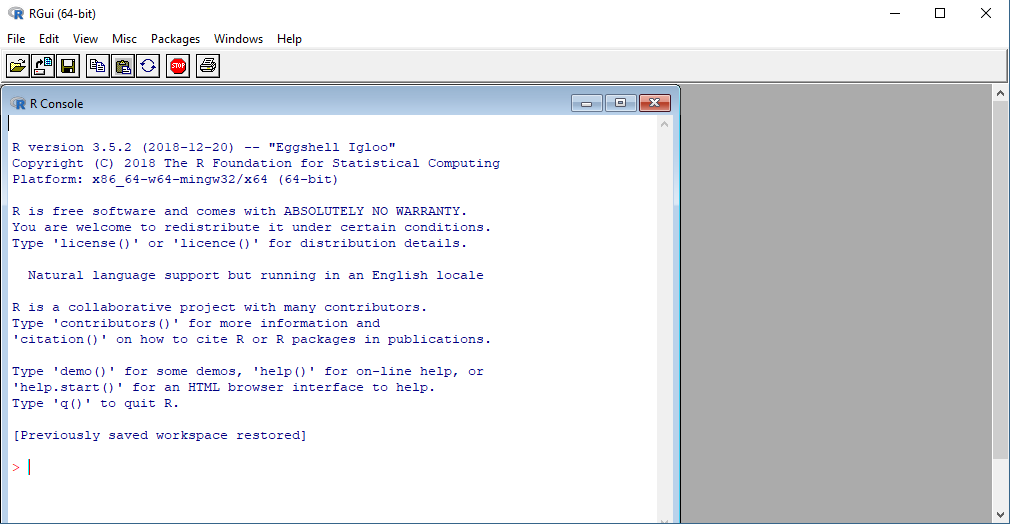
\includegraphics[width=0.8\linewidth]{./images/jendela_r} 

}

\caption{Jendela R.}\label{fig:jendela-R}
\end{figure}

\begin{figure}

{\centering 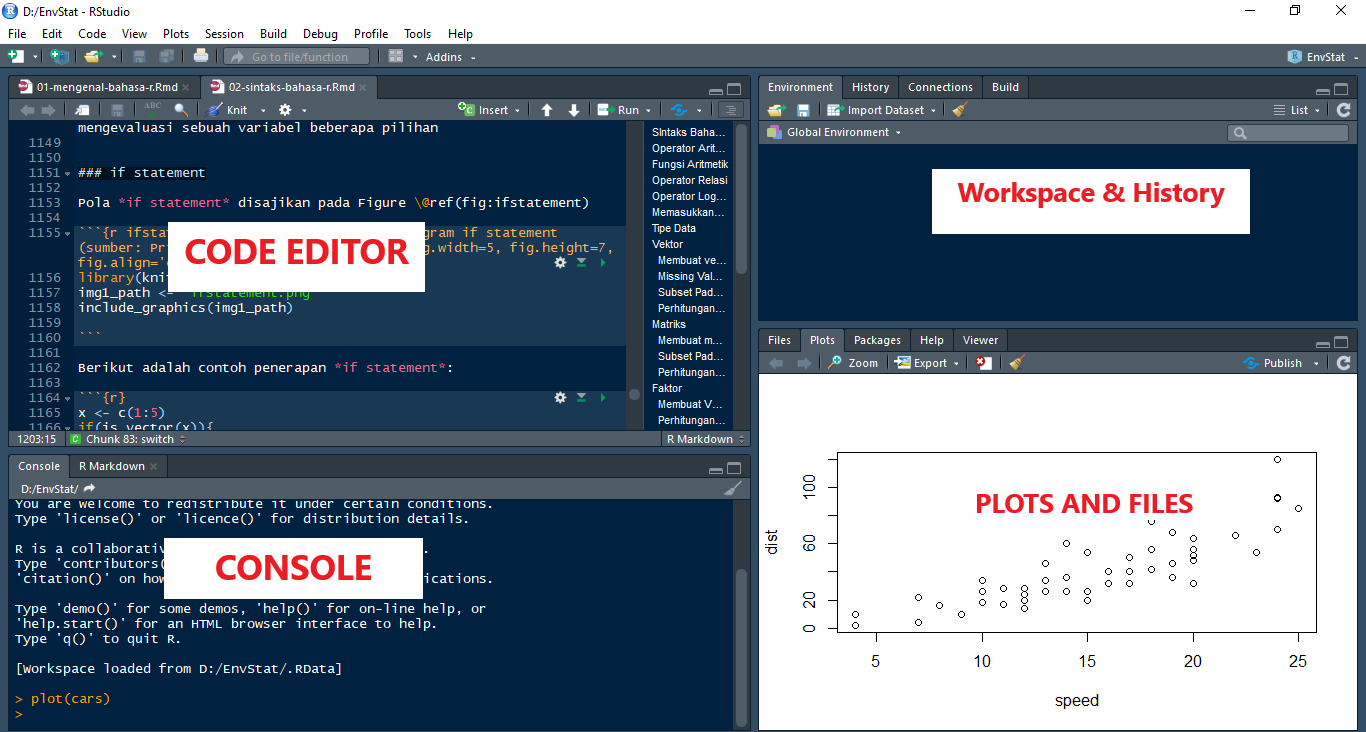
\includegraphics[width=0.8\linewidth]{./images/jendela_rstudio} 

}

\caption{Jendela RStudio.}\label{fig:jendela-RStudio}
\end{figure}

\begin{quote}
\textbf{Tips:} Sebaiknya install \texttt{R} terlebih dahulu sebelum \texttt{RStudio}
\end{quote}

\hypertarget{wdR}{%
\section{Working Directory}\label{wdR}}

Setiap pengguna akan bekerja pada tempat khusus yang disebut sebagai \emph{working directory}. \emph{working directory} merupakan sebuah folder dimana \texttt{R} akan membaca dan menyimpan file kerja kita. Pada pengguna \texttt{windows}, \emph{working directory} secara default pada saat pertama kali menginstall \texttt{R} terletak pada folder \texttt{c:\textbackslash{}\textbackslash{}Document}.

\hypertarget{changewdR}{%
\subsection{Mengubah Lokasi Working Directory}\label{changewdR}}

Kita dapat mengubah lokasi \emph{working directory} berdasarkan lokasi yang kita inginkan, misalnya letak data yang akan kita olah tidak ada pada folder default atau kita ingin pekerjaan kita terkait \texttt{R} dapat berlangsung pada satu folder khusus.

Berikut adalah cara mengubah \emph{working directory} pada \texttt{R}.

\begin{enumerate}
\def\labelenumi{\arabic{enumi}.}
\tightlist
\item
  Buatlah folder pada drive (kita bisa membuat folder pada selain drive c) dan namai dengan nama yang kalian inginkan. Pada tutorial ini penulis menggunakan nama folder \texttt{R}.
\item
  Jika pengguna menggunakan \texttt{RStudio}, pada menu \texttt{RStudio} pilih \textbf{Session \textgreater{} Set Working Directory \textgreater{} Chooses Directory}. Proses tersebut ditampilkan pada Gambar \ref{fig:working}
\item
  Pilih folder yang telah dibuat pada step 1 sebagai *working directory.
\end{enumerate}

\begin{quote}
\textbf{Penting:} Data atau file yang hendak dibaca selama proses kerja pada \texttt{R} harus selalu diletakkan pada working directory. Jika tidak maka data atau file tidak akan terbaca.
\end{quote}

Untuk mengecek apakah proses perubahan telah terjadi, kita dapat mengeceknya dengan menjalankan perintah berikut untuk melihat lokasi \emph{working directory} kita yang baru.

\begin{Shaded}
\begin{Highlighting}[]
\FunctionTok{getwd}\NormalTok{()}
\end{Highlighting}
\end{Shaded}

\begin{figure}

{\centering 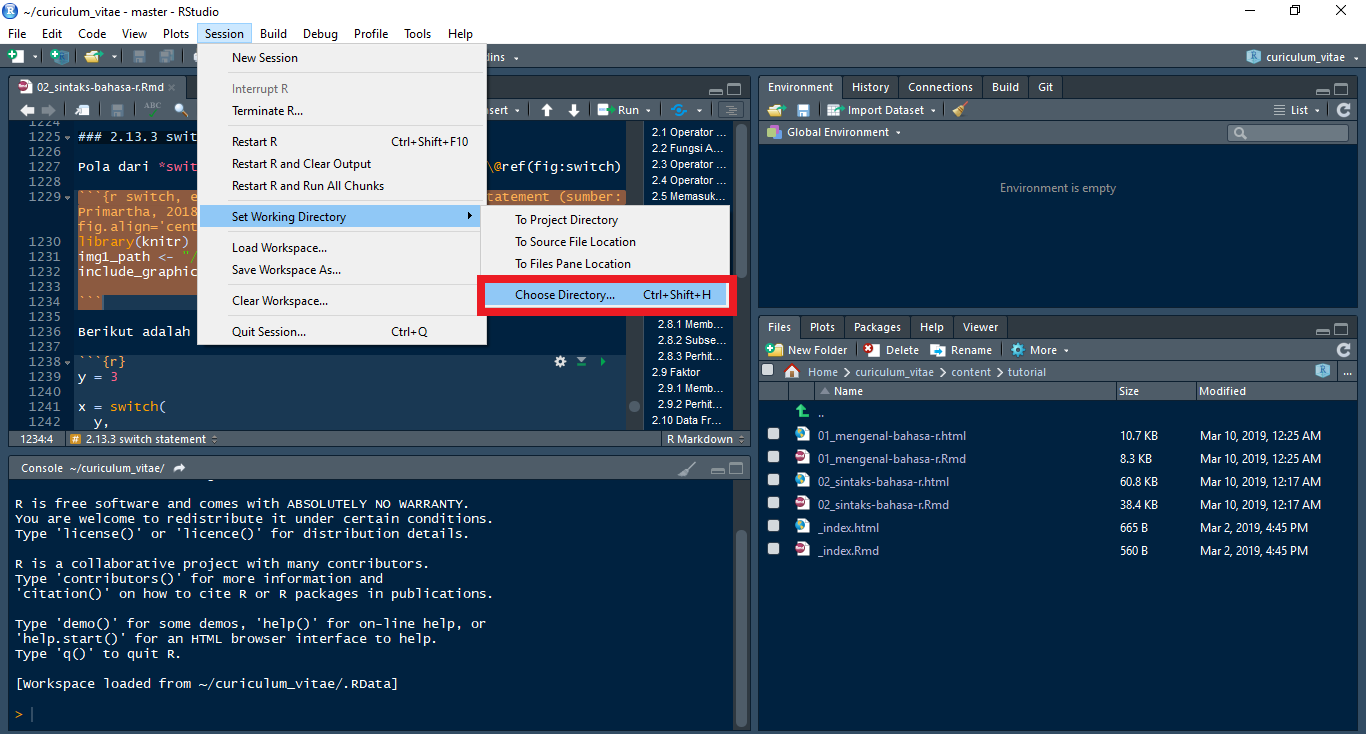
\includegraphics[width=0.8\linewidth]{./images/working} 

}

\caption{Mengubah working directory.}\label{fig:working}
\end{figure}

Selain itu kita dapat mengubah \emph{working directory} menggunakan perintah berikut:

\begin{Shaded}
\begin{Highlighting}[]
\CommentTok{\# Ubah working directori pada folder R}
\FunctionTok{setwd}\NormalTok{(}\StringTok{"/Documents/R"}\NormalTok{)}
\end{Highlighting}
\end{Shaded}

\begin{quote}
\textbf{Peringatan !!!}

Pada proses pengisian lokasi folder pastikan pemisah pada lokasi folder menggunakan tanda ``/'' bukan ``"
\end{quote}

\hypertarget{defaultwdR}{%
\subsection{Mengubah Lokasi Working Directory Default}\label{defaultwdR}}

Pada proses yang telah penulis jelaskan sebelumnya. Proses perubahan \emph{working directory} hanya berlaku pada saat pekerjaan tersebut dilakukan. Setelah pekerjaan selesai dan kita menjalankan kembali \texttt{R} maka \emph{working directory} akan kembali secara default pada working directory lama.

Untuk membuat lokasi default \emph{working directory} pindah, kita dapat melakukannya dengan memilih pada menu: \textbf{Tools \textgreater{} Global options \textgreater{} pada ``General'' klik pada ``Browse'' dan pilih lokasi working directory yang diinginkan}. Proses tersebut ditampilkan pada Gambar \ref{fig:default}

\begin{figure}

{\centering 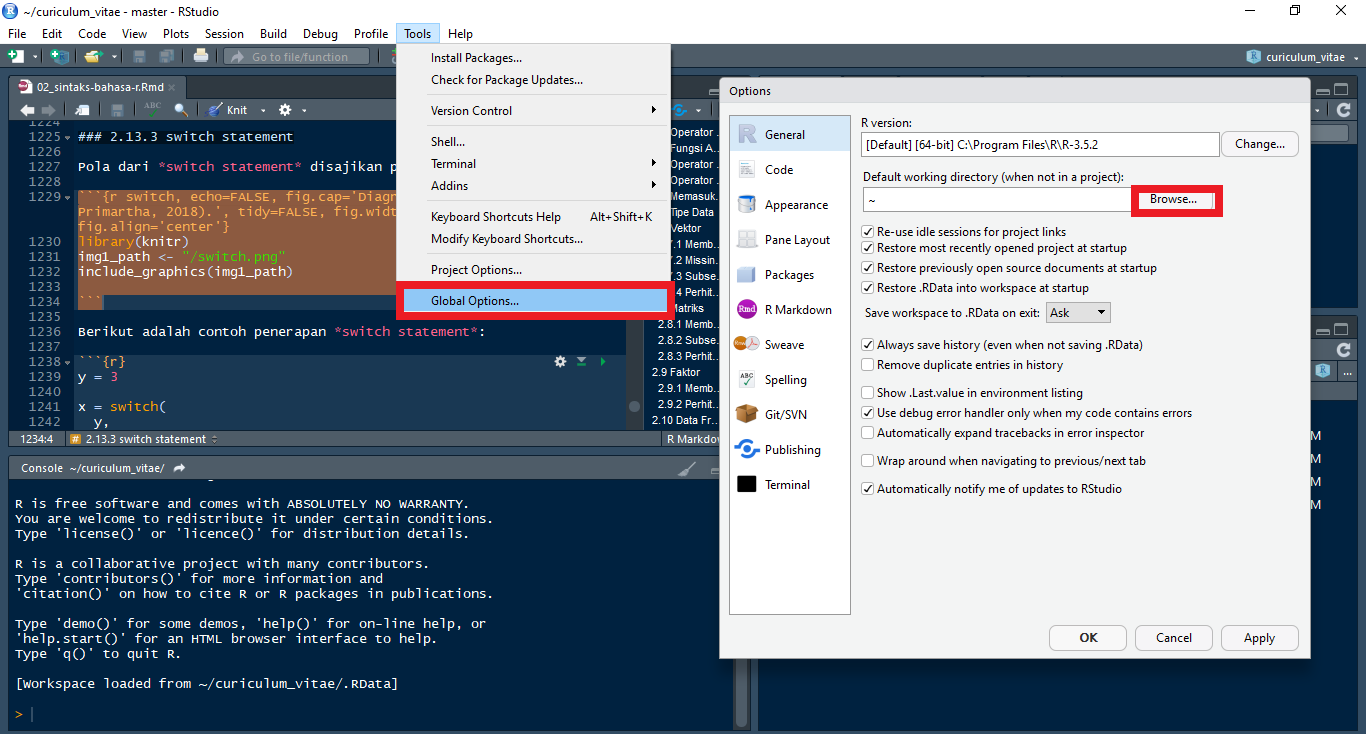
\includegraphics[width=0.8\linewidth]{./images/default} 

}

\caption{Merubah working directory melalui Global options.}\label{fig:default}
\end{figure}

\hypertarget{installlibraryR}{%
\section{Memasang dan Mengaktifkan Paket R}\label{installlibraryR}}

\texttt{R} dapat ditingkatkan fungsionalitasnya melalui Paket-Paket yang tersedia secara luas. Paket-Paket ini dikembangkan secara spesifik oleh para pengembang sesuai dengan tujuan paketnya, seperti: \texttt{tidyverse} untuk \emph{data science}, \texttt{pracma} untuk analisis diferensial, dll.

Untuk menginstall Paket yang kita inginkan, kita dapat menggunakan fungsi \texttt{install.packages()}. Berikut adalah contoh bagaimana cara menginstall Paket \texttt{tidyverse}:

\begin{Shaded}
\begin{Highlighting}[]
\FunctionTok{install.packages}\NormalTok{(}\StringTok{"tidyverse"}\NormalTok{)}
\end{Highlighting}
\end{Shaded}

Paket yang telah diinstall tidak dapat langsung digunakan. Untuk menggunakan fungsi-fungsi yang tersedia pada Paket tersebut kita perlu terlebih dahulu mengaktifkannya menggunakan fungsi \texttt{library()}. Berikut adalah contoh sintaks untuk mengaktifkan Paket \texttt{tidyverse}:

\begin{Shaded}
\begin{Highlighting}[]
\FunctionTok{library}\NormalTok{(tidyverse)}
\end{Highlighting}
\end{Shaded}

Bagaimana ingin menggunakan fungsi pada Paket namun tidak ingin mengaktifkan paketnya terlebih dahulu menggunakan fungsi \texttt{library()}? Untuk melakukannya kita perlu mengetikkan nama Paket dikuti oleh tanda ``::'' diikuti fungsi yang ingin kita gunakan. Berikut adalah contoh penggunaan fungsi \texttt{read\_csv()} dari Paket \texttt{readr} (salah satu Paket yang terdapat pada kumpulan Paket \texttt{tidyverse}) untuk membaca file \texttt{contoh.csv}:

\begin{Shaded}
\begin{Highlighting}[]
\NormalTok{readr}\SpecialCharTok{::}\FunctionTok{read\_csv}\NormalTok{(}\StringTok{"contoh.csv"}\NormalTok{)}
\end{Highlighting}
\end{Shaded}

\hypertarget{helpR}{%
\section{Fasilitas Help}\label{helpR}}

Agar dapat menggunakan \texttt{R} dengan secara lebih baik, pengetahuan untuk mengakses fasilitas \emph{help} in cukup penting untuk disampaikan. Adapun cara yang dapat digunakan adalah sebagai berikut.

\hypertarget{searchhelp}{%
\subsection{Mencari Help dari Suatu Perintah Tertentu}\label{searchhelp}}

Untuk memperoleh bantuan terkait suatu perintah tertentu kita dapat menggunakan fungsi \texttt{help()}. Secara umum format yang digunakan adalah sebagai berikut:

\begin{Shaded}
\begin{Highlighting}[]
\FunctionTok{help}\NormalTok{(nama\_perintah)}
\end{Highlighting}
\end{Shaded}

atau dapat juga menggunakan tanda tanya (?) pada awal \texttt{nama\_perintah} seperti berikut:

\begin{Shaded}
\begin{Highlighting}[]
\NormalTok{?nama\_perintah}
\end{Highlighting}
\end{Shaded}

Misalkan kita kebingungan terkait bagaimana cara menuliskan perintah untuk menghitung rata-rata suatu vektor. Kita dapat mengetikkan perintah berikut untuk mengakses fasilitas \emph{help}.

\begin{Shaded}
\begin{Highlighting}[]
\FunctionTok{help}\NormalTok{(mean)}

\CommentTok{\#atau}
\NormalTok{?mean}
\end{Highlighting}
\end{Shaded}

Perintah tersebut akan memunculkan hasil berupa dokumentasi yang ditampilkan pada Gambar \ref{fig:meandoc}.

\begin{figure}

{\centering 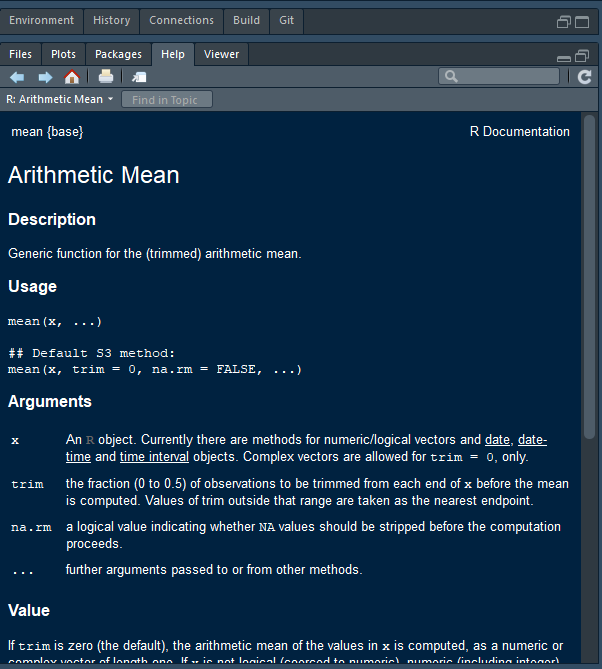
\includegraphics[width=0.5\linewidth]{./images/meandoc} 

}

\caption{Jendela help dokumentasi fungsi mean().}\label{fig:meandoc}
\end{figure}

Keterangan pada jendela pada Gambar \ref{fig:meandoc} adalah sebagia berikut:

\begin{enumerate}
\def\labelenumi{\arabic{enumi}.}
\tightlist
\item
  Pada bagian jendela kiri atas jendela \emph{help}, diberikan keterangan nama dari perintah yang sedang ditampilkan.
\item
  Selanjutnya, pada bagian atas dokumen, ditampilkan infomasi terkait nama perintah, dan nama Paket yang memuat perintah tersebut. Pada gambar diatas informasi terkait perintah dan nama Paket ditunjukkan pada teks \texttt{mean\ \{base\}} yang menunjukkan perintah \texttt{mean()} pada Paket (Paket) \emph{base} (Paket bawaan \texttt{R}).
\item
  Setiap jendela \emph{help} dari suatu perintah tertentu selanjutnya akan memuat bagian-bagian berikut:
\end{enumerate}

\begin{itemize}
\tightlist
\item
  \emph{Title}
\item
  \emph{Description} : deskripsi singkat tentang perintah.
\item
  \emph{Usage} : menampilkan sintaks perintah untuk penggunaan perintah tersebut.
\item
  \emph{Arguments} : keterangan mengenai \emph{argument/input}yang diperlukan pada perintah tersebut.
\item
  \emph{Details} : keterangan lebih lengkap lengkap tentang perintah tersebut.
\item
  \emph{Value} : keterangan tentang \emph{output} suatu perintah dapat diperoleh pada bagian ini.
\item
  \emph{Author(s)} : memberikan keterangan tentang \emph{Author} dari perintah tersebut.
\item
  \emph{References} : seringkali referensi yang dapat digunakan untuk memperoleh keterangan lebih lanjut terhadap suatu perintah ditampilkan pada bagian ini.
\item
  \emph{See also}: bagian ini berisikan daftar perintah/fungsi yang berhubungan erat dengan perintah tersebut.
\item
  \emph{Example} : berisikan contoh-contoh penggunaan perintah tersebut.
\end{itemize}

Kita juga dapat melihat contoh penggunaan dari perintah tersebut. Untuk melakukannya kita dapat menggunakan fungsi \texttt{example()}. Fungsi tersebut akan menampilkan contoh kode penerapan dari fungsi yang kita inginkan. Secara sederhana fungsi tersebut dapat dituliskan sebagai berikut:

\begin{Shaded}
\begin{Highlighting}[]
\FunctionTok{example}\NormalTok{(nama\_perintah)}
\end{Highlighting}
\end{Shaded}

Untuk mengetahui contoh kode fungsi \texttt{mean()}, ketikkan sintaks berikut:

\begin{Shaded}
\begin{Highlighting}[]
\FunctionTok{example}\NormalTok{(mean)}
\end{Highlighting}
\end{Shaded}

\begin{verbatim}
## 
## mean> x <- c(0:10, 50)
## 
## mean> xm <- mean(x)
## 
## mean> c(xm, mean(x, trim = 0.10))
## [1] 8.75 5.50
\end{verbatim}

kita juga dapat mencoba kode yang dihasilkan pada console \texttt{R}. Berikut adalah contoh penerapannya:

\begin{Shaded}
\begin{Highlighting}[]
\CommentTok{\# Menghitung rata{-}rata bilangan 1 sampai 10 dan 50}
\CommentTok{\# membuat vektor}
\NormalTok{x }\OtherTok{\textless{}{-}} \FunctionTok{c}\NormalTok{(}\DecValTok{0}\SpecialCharTok{:}\DecValTok{10}\NormalTok{, }\DecValTok{50}\NormalTok{)}

\CommentTok{\# Print}
\NormalTok{x}
\end{Highlighting}
\end{Shaded}

\begin{verbatim}
##  [1]  0  1  2  3  4  5  6  7  8  9 10 50
\end{verbatim}

\begin{Shaded}
\begin{Highlighting}[]
\CommentTok{\# mean}
\FunctionTok{mean}\NormalTok{(x)}
\end{Highlighting}
\end{Shaded}

\begin{verbatim}
## [1] 8.75
\end{verbatim}

Pembaca dapat mencoba melakukanya sendiri dengan mengganti nilai yang telah ada serta mencoba contoh kode yang lain.

\hypertarget{generalhelp}{%
\subsection{General Help}\label{generalhelp}}

Kita juga dapat membaca beberapa dokumen manual yang ada pada \texttt{R}. Untuk melakukannya jalankan perintah berikut:

\begin{Shaded}
\begin{Highlighting}[]
\FunctionTok{help.start}\NormalTok{()}
\end{Highlighting}
\end{Shaded}

Output yang dihasilkan berupa link pada sejumlah dokumen yang dapat kita klik. Tampilan halaman yang dihasilkan disajikan pada Gambar \ref{fig:generalhelp}.

\begin{figure}

{\centering 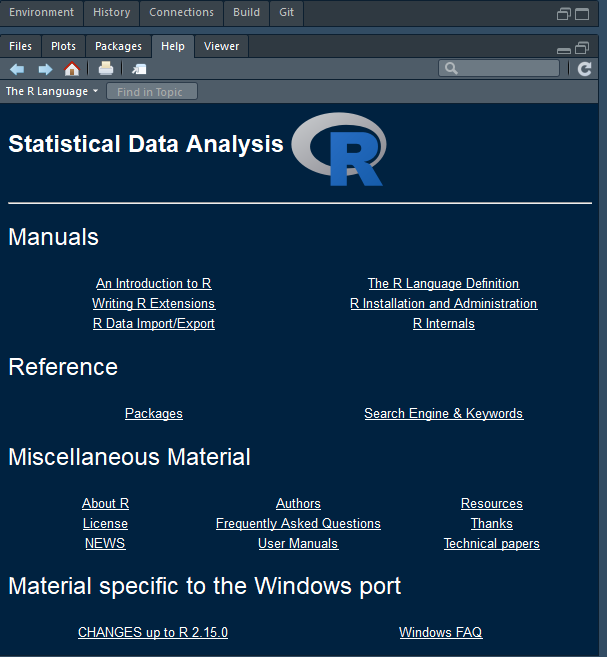
\includegraphics[width=0.5\linewidth]{./images/generalhelp} 

}

\caption{Jendela general help dokumentasi fungsi mean().}\label{fig:generalhelp}
\end{figure}

\hypertarget{othershelp}{%
\subsection{Fasilitas Help Lainnya}\label{othershelp}}

Selain yang telah penulis sebutkan sebelumnya. Kita juga dapat memanfaatkan fasilitas \emph{help} lainnya melalui fungsi \texttt{apropos()} dan \texttt{help.search()}.

\texttt{apropos\ ()}: mengembalikan daftar objek, berisi pola yang pembaca cari, dengan pencocokan sebagian. Ini berguna ketika pembaca tidak ingat persis nama fungsi yang akan digunakan. Berikut adalah contoh ketika penulis ingin mengetahui fungsi yang digunakan untuk menghitung median.

\begin{Shaded}
\begin{Highlighting}[]
\FunctionTok{apropos}\NormalTok{(}\StringTok{"med"}\NormalTok{)}
\end{Highlighting}
\end{Shaded}

\begin{verbatim}
## [1] "elNamed"        "elNamed<-"      "median"        
## [4] "median.default" "medpolish"      "runmed"
\end{verbatim}

\emph{List} yang dihasilkan berupa fungsi-fungsi yang memiliki elemen kata ``med''. Berdasarkan pencaria tersebut penulis dapat mencoba menggunakan fungsi ``median'' untuk menghitung median.

\texttt{help.search\ ()} (sebagai alternatif ??): mencari dokumentasi yang cocok dengan karakter yang diberikan dengan cara yang berbeda. Ini mengembalikan daftar fungsi yang mengandung istilah yang pembaca cari dengan deskripsi singkat dari fungsi.

Berikut adalah contoh penerapan dari fungsi tersebut:

\begin{Shaded}
\begin{Highlighting}[]
\FunctionTok{help.search}\NormalTok{(}\StringTok{"mean"}\NormalTok{)}

\CommentTok{\# atau}
\NormalTok{??mean}
\end{Highlighting}
\end{Shaded}

\emph{Output} yang dihasilkan akan tampak seperti pada Gambar \ref{fig:helpsearch}.

\begin{figure}

{\centering 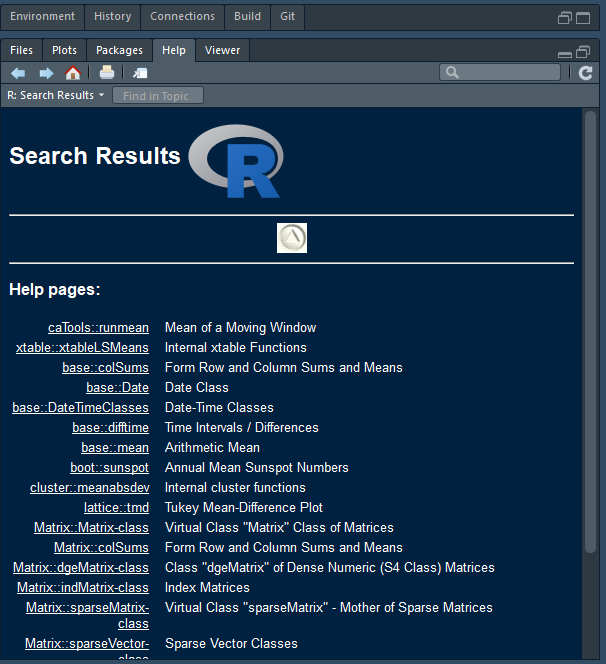
\includegraphics[width=0.5\linewidth]{./images/helpsearch} 

}

\caption{Jendela help search dokumentasi fungsi mean().}\label{fig:helpsearch}
\end{figure}

\hypertarget{referensi}{%
\section{Referensi}\label{referensi}}

\begin{enumerate}
\def\labelenumi{\arabic{enumi}.}
\tightlist
\item
  Primartha, R. 2018. \textbf{Belajar Machine Learning Teori dan Praktik}. Penerbit Informatika : Bandung
\item
  Rosadi,D. 2016. \textbf{Analisis Statistika dengan R}. Gadjah Mada University Press: Yogyakarta
\item
  STHDA. Running RStudio and Setting Up Your Working Directory - Easy R Programming .\url{http://www.sthda.com/english/wiki/running-rstudio-and-setting-up-your-working-directory-easy-r-programming\#set-your-working-directory}
\item
  STDHA. \textbf{Getting Help With Functions In R Programming}. \url{http://www.sthda.com/english/wiki/getting-help-with-functions-in-r-programming} .
\item
  Venables, W.N. Smith D.M. and R Core Team. 2018. \textbf{An Introduction to R}. R Manuals.
\end{enumerate}

\hypertarget{calculation}{%
\chapter{Kalkulasi Menggunakan R}\label{calculation}}

Pada \emph{Chapter} ini penulis akan menjelaskan bagaimana melakukan perhitungan menggunakan \texttt{R}. Hal-hal yang akan dibahas pada \emph{chapter} ini antara lain:

\begin{itemize}
\tightlist
\item
  Operator dan fungsi dasar pada \texttt{R}
\item
  Jenis dan struktur data
\item
  Vektor (cara membuat dan melakukan operasi matematika pada vektor)
\item
  Matriks (cara membuat dan melakukan operasi matematika pada matriks)
\end{itemize}

\hypertarget{aritmetikoperator}{%
\section{Operator Aritmatik}\label{aritmetikoperator}}

Proses perhitungan akan ditangani oleh fungsi khusus. \texttt{R} akan memahami urutannya secara benar. Kecuali kita secara eksplisit menetapkan yang lain. Sebagai contoh jalankan sintaks berikut:

\begin{Shaded}
\begin{Highlighting}[]
\DecValTok{2}\SpecialCharTok{+}\DecValTok{4}\SpecialCharTok{*}\DecValTok{2}
\end{Highlighting}
\end{Shaded}

\begin{verbatim}
## [1] 10
\end{verbatim}

Bandingkan dengan sintaks berikut:

\begin{Shaded}
\begin{Highlighting}[]
\NormalTok{(}\DecValTok{2}\SpecialCharTok{+}\DecValTok{4}\NormalTok{)}\SpecialCharTok{*}\DecValTok{2}
\end{Highlighting}
\end{Shaded}

\begin{verbatim}
## [1] 12
\end{verbatim}

\begin{quote}
\textbf{Tips:} \texttt{R} dapat digunakan sebagai kalkulator
\end{quote}

Berdasarkan kedua hasil tersebut dapat disimpulkan bahwa ketika kita tidak menetapkan urutan perhitungan menggunakan tanda kurung, \texttt{R} akan secara otomatis akan menghitung terlebih dahulu perkalian atau pembangian.

Operator aritmatika yang disediakan \texttt{R} disajikan pada Tabel \ref{tab:oparitmatika}:

\begin{longtable}[]{@{}
  >{\raggedright\arraybackslash}p{(\columnwidth - 2\tabcolsep) * \real{0.1485}}
  >{\raggedright\arraybackslash}p{(\columnwidth - 2\tabcolsep) * \real{0.8515}}@{}}
\caption{\label{tab:oparitmatika} Operator Aritmatika \texttt{R}.}\tabularnewline
\toprule\noalign{}
\begin{minipage}[b]{\linewidth}\raggedright
\textbf{Simbol}
\end{minipage} & \begin{minipage}[b]{\linewidth}\raggedright
\textbf{Keterangan}
\end{minipage} \\
\midrule\noalign{}
\endfirsthead
\toprule\noalign{}
\begin{minipage}[b]{\linewidth}\raggedright
\textbf{Simbol}
\end{minipage} & \begin{minipage}[b]{\linewidth}\raggedright
\textbf{Keterangan}
\end{minipage} \\
\midrule\noalign{}
\endhead
\bottomrule\noalign{}
\endlastfoot
+ & \emph{Addition}, untuk operasi penjumlahan \\
- & \emph{Substraction}, untuk operasi pengurangan \\
* & \emph{Multiplication}, untuk operasi pembagian \\
/ & \emph{Division}, untuk operasi pembagian \\
\^{} & \emph{Eksponentiation}, untuk operasi pemangkatan \\
\%\% & \emph{Modulus}, Untuk mencari sisa pembagian \\
\%/\% & \emph{Integer}, Untuk mencari bilangan bulat hasil pembagian saja dan tanpa sisa pembagian \\
\end{longtable}

Untuk lebih memahaminya berikut contoh sintaks penerapan operator tersebut.

\begin{Shaded}
\begin{Highlighting}[]
\CommentTok{\# Addition}
\DecValTok{5}\SpecialCharTok{+}\DecValTok{3}
\end{Highlighting}
\end{Shaded}

\begin{verbatim}
## [1] 8
\end{verbatim}

\begin{Shaded}
\begin{Highlighting}[]
\CommentTok{\# Substraction}
\DecValTok{5{-}3}
\end{Highlighting}
\end{Shaded}

\begin{verbatim}
## [1] 2
\end{verbatim}

\begin{Shaded}
\begin{Highlighting}[]
\CommentTok{\# Multiplication}
\DecValTok{5}\SpecialCharTok{*}\DecValTok{3}
\end{Highlighting}
\end{Shaded}

\begin{verbatim}
## [1] 15
\end{verbatim}

\begin{Shaded}
\begin{Highlighting}[]
\CommentTok{\# Division}
\DecValTok{5}\SpecialCharTok{/}\DecValTok{3}
\end{Highlighting}
\end{Shaded}

\begin{verbatim}
## [1] 1.667
\end{verbatim}

\begin{Shaded}
\begin{Highlighting}[]
\CommentTok{\# Eksponetiation}
\DecValTok{5}\SpecialCharTok{\^{}}\DecValTok{3}
\end{Highlighting}
\end{Shaded}

\begin{verbatim}
## [1] 125
\end{verbatim}

\begin{Shaded}
\begin{Highlighting}[]
\CommentTok{\# Modulus}
\DecValTok{5}\SpecialCharTok{\%\%}\DecValTok{3}
\end{Highlighting}
\end{Shaded}

\begin{verbatim}
## [1] 2
\end{verbatim}

\begin{Shaded}
\begin{Highlighting}[]
\CommentTok{\# Integer}
\DecValTok{5}\SpecialCharTok{\%/\%}\DecValTok{3}
\end{Highlighting}
\end{Shaded}

\begin{verbatim}
## [1] 1
\end{verbatim}

\begin{quote}
\textbf{Tips:} Pada \texttt{R} tanda \texttt{\#} berfungsi menambahkan keterangan untuk menjelaskan sebuah sintaks pada \texttt{R}
\end{quote}

\hypertarget{aritmaticfunction}{%
\section{Fungsi Aritmetik}\label{aritmaticfunction}}

Selain fungsi operator aritmetik, pada \texttt{R} juga telah tersedia fungsi aritmetik yang lain seperti logaritmik, ekponensial, trigonometri, dll.

\begin{enumerate}
\def\labelenumi{\arabic{enumi}.}
\tightlist
\item
  Logaritma dan eksponensial
\end{enumerate}

Untuk contoh fungsi logaritmik dan eksponensial jalankan sintaks berikut:

\begin{Shaded}
\begin{Highlighting}[]
\FunctionTok{log2}\NormalTok{(}\DecValTok{8}\NormalTok{) }\CommentTok{\# logaritma basis 2 untuk 8}
\end{Highlighting}
\end{Shaded}

\begin{verbatim}
## [1] 3
\end{verbatim}

\begin{Shaded}
\begin{Highlighting}[]
\FunctionTok{log10}\NormalTok{(}\DecValTok{8}\NormalTok{) }\CommentTok{\# logaritma basis 10 untuk 8}
\end{Highlighting}
\end{Shaded}

\begin{verbatim}
## [1] 0.9031
\end{verbatim}

\begin{Shaded}
\begin{Highlighting}[]
\FunctionTok{exp}\NormalTok{(}\DecValTok{8}\NormalTok{) }\CommentTok{\# eksponensial 8}
\end{Highlighting}
\end{Shaded}

\begin{verbatim}
## [1] 2981
\end{verbatim}

\begin{enumerate}
\def\labelenumi{\arabic{enumi}.}
\setcounter{enumi}{1}
\tightlist
\item
  Fungsi trigonometri
\end{enumerate}

fungsi trigonometri yang ditampilkan seperti sin,cos, tan, dll.

\begin{Shaded}
\begin{Highlighting}[]
\FunctionTok{cos}\NormalTok{(x) }\CommentTok{\# cos x}
\FunctionTok{sin}\NormalTok{(x) }\CommentTok{\# Sin x}
\FunctionTok{tan}\NormalTok{(x) }\CommentTok{\# Tan x}
\FunctionTok{acos}\NormalTok{(x) }\CommentTok{\# arc{-}cos x}
\FunctionTok{asin}\NormalTok{(x) }\CommentTok{\# arc{-}sin x}
\FunctionTok{atan}\NormalTok{(x) }\CommentTok{\#arc{-}tan x}
\end{Highlighting}
\end{Shaded}

\begin{quote}
\textbf{Penting!!!}

x dalam fungsi trigonometri memiliki satuan radian
\end{quote}

Berikut adalah salah satu contoh penggunaannya:

\begin{Shaded}
\begin{Highlighting}[]
\FunctionTok{cos}\NormalTok{(pi)}
\end{Highlighting}
\end{Shaded}

\begin{verbatim}
## [1] -1
\end{verbatim}

Pada Paket \texttt{pracma} fungsi-fungsi trigonometri dapat ditambah lagi. Fungsi-fungsi tersebut antara lain:

\begin{Shaded}
\begin{Highlighting}[]
\FunctionTok{cot}\NormalTok{(x) }\CommentTok{\# cotan x}
\FunctionTok{csc}\NormalTok{(x) }\CommentTok{\# cosecan x}
\FunctionTok{sec}\NormalTok{(x) }\CommentTok{\# secan x}
\FunctionTok{acot}\NormalTok{(x) }\CommentTok{\# arc{-}cotan x}
\FunctionTok{acsc}\NormalTok{(x) }\CommentTok{\# arc{-}cosecan x}
\FunctionTok{asec}\NormalTok{(x) }\CommentTok{\# arc{-}secan x}
\end{Highlighting}
\end{Shaded}

\begin{enumerate}
\def\labelenumi{\arabic{enumi}.}
\setcounter{enumi}{2}
\tightlist
\item
  Fungsi Hiperbolik
\end{enumerate}

fungsi hiperbolik yang tersedia antara lain:

\begin{Shaded}
\begin{Highlighting}[]
\FunctionTok{cosh}\NormalTok{(x) }
\FunctionTok{sinh}\NormalTok{(x)}
\FunctionTok{tanh}\NormalTok{(x)}
\FunctionTok{acosh}\NormalTok{(x)}
\FunctionTok{asinh}\NormalTok{(x)}
\FunctionTok{atanh}\NormalTok{(x)}
\end{Highlighting}
\end{Shaded}

Fungsi tersebut dapat ditambah lagi dari Paket \texttt{pracma}. Fungsi-fungsi yang tersedia antara lain:

\begin{Shaded}
\begin{Highlighting}[]
\FunctionTok{coth}\NormalTok{(x)}
\FunctionTok{csch}\NormalTok{(x)}
\FunctionTok{sech}\NormalTok{(x)}
\FunctionTok{acoth}\NormalTok{(x)}
\FunctionTok{acsch}\NormalTok{(x)}
\FunctionTok{asech}\NormalTok{(x)}
\end{Highlighting}
\end{Shaded}

\begin{enumerate}
\def\labelenumi{\arabic{enumi}.}
\setcounter{enumi}{3}
\tightlist
\item
  Fungsi matematik lainnya
\end{enumerate}

Fungsi lainnya yang dapat digunakan adalah fungsi absolut, akar kuadrat, dll. Berikut adalah contoh sintaks penggunaan fungsi absolut dan akar kuadrat.

\begin{Shaded}
\begin{Highlighting}[]
\FunctionTok{abs}\NormalTok{(}\SpecialCharTok{{-}}\DecValTok{2}\NormalTok{) }\CommentTok{\# nilai absolut {-}2}
\end{Highlighting}
\end{Shaded}

\begin{verbatim}
## [1] 2
\end{verbatim}

\begin{Shaded}
\begin{Highlighting}[]
\FunctionTok{sqrt}\NormalTok{(}\DecValTok{4}\NormalTok{) }\CommentTok{\# akar kuadrat 4}
\end{Highlighting}
\end{Shaded}

\begin{verbatim}
## [1] 2
\end{verbatim}

\hypertarget{relationoperators}{%
\section{Operator Relasi}\label{relationoperators}}

Operator relasi digunakan untuk membandingkan satu objek dengan objek lainnya. Operator yang disediakan \texttt{R} disajikan pada Tabel \ref{tab:oprelasi}.

\begin{longtable}[]{@{}ll@{}}
\caption{\label{tab:oprelasi} Operator Relasi \texttt{R}.}\tabularnewline
\toprule\noalign{}
\textbf{Simbol} & \textbf{Keterangan} \\
\midrule\noalign{}
\endfirsthead
\toprule\noalign{}
\textbf{Simbol} & \textbf{Keterangan} \\
\midrule\noalign{}
\endhead
\bottomrule\noalign{}
\endlastfoot
``\textgreater{}'' & Lebih besar dari \\
``\textless{}'' & Lebih Kecil dari \\
``=='' & Sama dengan \\
``\textgreater='' & Lebih besar sama dengan \\
``\textless='' & Lebih kecil sama dengan \\
``!='' & Tidak sama dengan \\
\end{longtable}

Berikut adalah penerapan operator pada tabel tersebut:

\begin{Shaded}
\begin{Highlighting}[]
\NormalTok{x }\OtherTok{\textless{}{-}} \DecValTok{34}
\NormalTok{y }\OtherTok{\textless{}{-}} \DecValTok{35}

\CommentTok{\# Operator \textgreater{}}
\NormalTok{x }\SpecialCharTok{\textgreater{}}\NormalTok{ y}
\end{Highlighting}
\end{Shaded}

\begin{verbatim}
## [1] FALSE
\end{verbatim}

\begin{Shaded}
\begin{Highlighting}[]
\CommentTok{\# Operator \textless{}}
\NormalTok{x }\SpecialCharTok{\textless{}}\NormalTok{ y}
\end{Highlighting}
\end{Shaded}

\begin{verbatim}
## [1] TRUE
\end{verbatim}

\begin{Shaded}
\begin{Highlighting}[]
\CommentTok{\# operator ==}
\NormalTok{x }\SpecialCharTok{==}\NormalTok{ y}
\end{Highlighting}
\end{Shaded}

\begin{verbatim}
## [1] FALSE
\end{verbatim}

\begin{Shaded}
\begin{Highlighting}[]
\CommentTok{\# Operator \textgreater{}=}
\NormalTok{x }\SpecialCharTok{\textgreater{}=}\NormalTok{ y}
\end{Highlighting}
\end{Shaded}

\begin{verbatim}
## [1] FALSE
\end{verbatim}

\begin{Shaded}
\begin{Highlighting}[]
\CommentTok{\# Operator \textless{}=}
\NormalTok{x }\SpecialCharTok{\textless{}=}\NormalTok{ y}
\end{Highlighting}
\end{Shaded}

\begin{verbatim}
## [1] TRUE
\end{verbatim}

\begin{Shaded}
\begin{Highlighting}[]
\CommentTok{\# Operator !=}
\NormalTok{x }\SpecialCharTok{!=}\NormalTok{ y}
\end{Highlighting}
\end{Shaded}

\begin{verbatim}
## [1] TRUE
\end{verbatim}

\hypertarget{logicoperators}{%
\section{Operator Logika}\label{logicoperators}}

Operator logika hanya berlaku pada vektor dengan tipe logical, numeric, atau complex. Semua angka bernilai 1 akan dianggap bernilai logika \texttt{TRUE}. Operator logika yang disediakan \texttt{R} dapat dilihat pada Tabel \ref{tab:oplogika}.

\begin{longtable}[]{@{}ll@{}}
\caption{\label{tab:oplogika} Operator logika \texttt{R}.}\tabularnewline
\toprule\noalign{}
\textbf{Simbol} & \textbf{Keterangan} \\
\midrule\noalign{}
\endfirsthead
\toprule\noalign{}
\textbf{Simbol} & \textbf{Keterangan} \\
\midrule\noalign{}
\endhead
\bottomrule\noalign{}
\endlastfoot
``\&\&'' & Operator logika AND \\
'' & \\
``!'' & Opeartor logika NOT \\
``\&'' & Operator logika AND element wise \\
'' & '' \\
\end{longtable}

Penerapannya terdapat pada sintaks berikut:

\begin{Shaded}
\begin{Highlighting}[]
\NormalTok{v }\OtherTok{\textless{}{-}} \FunctionTok{c}\NormalTok{(}\ConstantTok{TRUE}\NormalTok{,}\ConstantTok{TRUE}\NormalTok{, }\ConstantTok{FALSE}\NormalTok{)}
\NormalTok{t }\OtherTok{\textless{}{-}} \FunctionTok{c}\NormalTok{(}\ConstantTok{FALSE}\NormalTok{,}\ConstantTok{FALSE}\NormalTok{,}\ConstantTok{FALSE}\NormalTok{)}

\CommentTok{\# Operator !}
\FunctionTok{print}\NormalTok{(}\SpecialCharTok{!}\NormalTok{v)}
\end{Highlighting}
\end{Shaded}

\begin{verbatim}
## [1] FALSE FALSE  TRUE
\end{verbatim}

\begin{Shaded}
\begin{Highlighting}[]
\CommentTok{\# operator \&}
\FunctionTok{print}\NormalTok{(v}\SpecialCharTok{\&}\NormalTok{t)}
\end{Highlighting}
\end{Shaded}

\begin{verbatim}
## [1] FALSE FALSE FALSE
\end{verbatim}

\begin{Shaded}
\begin{Highlighting}[]
\CommentTok{\# Operator |}
\FunctionTok{print}\NormalTok{(v}\SpecialCharTok{|}\NormalTok{t)}
\end{Highlighting}
\end{Shaded}

\begin{verbatim}
## [1]  TRUE  TRUE FALSE
\end{verbatim}

\begin{quote}
\textbf{Penting!!!}

\begin{itemize}
\tightlist
\item
  operator \texttt{\&} dan \texttt{\textbar{}} akan mengecek logika tiap elemen pada vektor secara berpesangan (sesuai urutan dari kiri ke kanan).
  Operator \texttt{\%\%} dan \texttt{\textbar{}\textbar{}} hanya mengecek dari kiri ke kanan pada
\item
  observasi pertama. Misal saat menggunakan \&\& jika observasi pertama \texttt{TRUE} maka observasi pertama pada vektor lainnya akan dicek, namun jika observasi pertama \texttt{FALSE} maka proses akan segera dihentikan dan menghasilkan FALSE.
\end{itemize}
\end{quote}

\hypertarget{assigningvar}{%
\section{Memasukkan Nilai Kedalam Variabel}\label{assigningvar}}

Variabel pada \texttt{R} dapat digunakan untuk menyimpan nilai. Sebagai contoh jalankan sintaks berikut:

\begin{Shaded}
\begin{Highlighting}[]
\CommentTok{\# Harga sebuah lemon adalah 500 rupiah}
\NormalTok{lemon }\OtherTok{\textless{}{-}} \DecValTok{500}

\CommentTok{\# Atau}
\DecValTok{500} \OtherTok{{-}\textgreater{}}\NormalTok{ lemon}

\CommentTok{\# dapat juga menggunakan tanda "="}
\NormalTok{lemon }\OtherTok{=} \DecValTok{500}
\end{Highlighting}
\end{Shaded}

\begin{quote}
\textbf{Penting!!!}

\begin{enumerate}
\def\labelenumi{\arabic{enumi}.}
\tightlist
\item
  \texttt{R} memungkinkan penggunaan \texttt{\textless{}-},\texttt{-\textgreater{}}, atau \texttt{=} sebagai perintah pengisi nilai variabel
\item
  \texttt{R} bersifat \emph{case-sensitive}. Maksudnya adalah variabel Lemon tidak sama dengan lemon (Besar kecil huruf berpengaruh)
\end{enumerate}
\end{quote}

Untuk mengetahui nilai dari objek \texttt{lemon} kita dapat menggunakan fungsi \texttt{print()} atau mengetikkan nama objeknya secara langsung.

\begin{Shaded}
\begin{Highlighting}[]
\CommentTok{\# Menggunakan fungsi print()}
\FunctionTok{print}\NormalTok{(lemon)}
\end{Highlighting}
\end{Shaded}

\begin{verbatim}
## [1] 500
\end{verbatim}

\begin{Shaded}
\begin{Highlighting}[]
\CommentTok{\# Atau}
\NormalTok{lemon}
\end{Highlighting}
\end{Shaded}

\begin{verbatim}
## [1] 500
\end{verbatim}

\texttt{R} akan menyimpan variabel \texttt{lemon} sebagai objek pada memori. Sehingga kita dapat melakukan operasi terhadap objek tersebut seperti mengalikannya atau menjumlahkannya dengan bilangan lain. Sebagai contoh jalankan sintaks berikut:

\begin{Shaded}
\begin{Highlighting}[]
\CommentTok{\# Operasi perkalian terhadap objek lemon}
\DecValTok{5}\SpecialCharTok{*}\NormalTok{lemon}
\end{Highlighting}
\end{Shaded}

\begin{verbatim}
## [1] 2500
\end{verbatim}

Kita dapat juga mengubah nilai dari objek \texttt{lemon} dengan cara menginput nilai baru terhadap objek yang sama. \texttt{R} secara otomatis akan menggatikan nilai sebelumnya. Untuk lebih memahaminya jalankan sintaks berikut:

\begin{Shaded}
\begin{Highlighting}[]
\NormalTok{lemon }\OtherTok{\textless{}{-}} \DecValTok{1000}

\CommentTok{\# Print lemon}
\FunctionTok{print}\NormalTok{(lemon)}
\end{Highlighting}
\end{Shaded}

\begin{verbatim}
## [1] 1000
\end{verbatim}

Untuk lebih memahaminya berikut adalah sintaks untuk menghitung volume suatu objek.

\begin{Shaded}
\begin{Highlighting}[]
\CommentTok{\# Dimensi objek}
\NormalTok{panjang }\OtherTok{\textless{}{-}} \DecValTok{10}
\NormalTok{lebar }\OtherTok{\textless{}{-}} \DecValTok{5}
\NormalTok{tinggi }\OtherTok{\textless{}{-}} \DecValTok{5}

\CommentTok{\# Menghitung volume}
\NormalTok{volume }\OtherTok{\textless{}{-}}\NormalTok{ panjang}\SpecialCharTok{*}\NormalTok{lebar}\SpecialCharTok{*}\NormalTok{tinggi}

\CommentTok{\# Print objek volume}
\FunctionTok{print}\NormalTok{(volume)}
\end{Highlighting}
\end{Shaded}

\begin{verbatim}
## [1] 250
\end{verbatim}

Untuk mengetahui objek apa saja yang telah kita buat sepanjang artikel ini kita dapang menggunakan fungsi \texttt{ls()}.

\begin{Shaded}
\begin{Highlighting}[]
\FunctionTok{ls}\NormalTok{()}
\end{Highlighting}
\end{Shaded}

\begin{verbatim}
##  [1] "A"         "B"         "img1_path" "lebar"    
##  [5] "lemon"     "panjang"   "t"         "tinggi"   
##  [9] "v"         "volume"    "x"         "xm"       
## [13] "y"
\end{verbatim}

\begin{quote}
\textbf{Catatan:} Kumpulan objek yang telah tersimpan dalam memori disebut sebagai \textbf{workspace}
\end{quote}

Untuk menghapus objek pada memori kita dapat menggunakan fungsi \texttt{rm()}. Pada sintaks berikut penulis hendak menghapus objek \texttt{lemon} dan \texttt{volume}.

\begin{Shaded}
\begin{Highlighting}[]
\CommentTok{\# Menghapus objek lemon dan volume}
\FunctionTok{rm}\NormalTok{(lemon, volume)}

\CommentTok{\# Tampilkan kembali objek yang tersisa}
\FunctionTok{ls}\NormalTok{()}
\end{Highlighting}
\end{Shaded}

\begin{verbatim}
##  [1] "A"         "B"         "img1_path" "lebar"    
##  [5] "panjang"   "t"         "tinggi"    "v"        
##  [9] "x"         "xm"        "y"
\end{verbatim}

\begin{quote}
\textbf{Tips:} Setiap variabel atau objek yang dibuat akan menempati sejumlah memori pada komputer sehingga jika kita bekerja dengan jumlah data yang banyak pastikan kita menghapus seluruh objek pada memori sebelum memulai kerja.
\end{quote}

\hypertarget{typedata}{%
\section{Tipe dan Struktur Data}\label{typedata}}

Data pada \texttt{R} dapat dikelompokan berdasarkan beberapa tipe. Tipe data pada \texttt{R} disajikan pada Tabel \ref{tab:tipedata}.

\begin{longtable}[]{@{}
  >{\raggedright\arraybackslash}p{(\columnwidth - 4\tabcolsep) * \real{0.1240}}
  >{\raggedright\arraybackslash}p{(\columnwidth - 4\tabcolsep) * \real{0.2066}}
  >{\raggedright\arraybackslash}p{(\columnwidth - 4\tabcolsep) * \real{0.6694}}@{}}
\caption{\label{tab:tipedata} Tipe data \texttt{R}.}\tabularnewline
\toprule\noalign{}
\begin{minipage}[b]{\linewidth}\raggedright
\textbf{Tipe Data}
\end{minipage} & \begin{minipage}[b]{\linewidth}\raggedright
\textbf{Contoh}
\end{minipage} & \begin{minipage}[b]{\linewidth}\raggedright
\textbf{Keterangan}
\end{minipage} \\
\midrule\noalign{}
\endfirsthead
\toprule\noalign{}
\begin{minipage}[b]{\linewidth}\raggedright
\textbf{Tipe Data}
\end{minipage} & \begin{minipage}[b]{\linewidth}\raggedright
\textbf{Contoh}
\end{minipage} & \begin{minipage}[b]{\linewidth}\raggedright
\textbf{Keterangan}
\end{minipage} \\
\midrule\noalign{}
\endhead
\bottomrule\noalign{}
\endlastfoot
Logical & TRUE, FALSE & Nilai Boolean \\
Numeric & 12.3, 5, 999 & Segala jenis angka \\
Integer & 23L, 97L, 3L & Bilangan integer (bilangan bulat) \\
Complex & 2i, 3i, 9i & Bilangan kompleks \\
Character & `a', ``b'', ``123'' & Karakter dan string \\
Factor & 1, 0, ``Merah'' & Dapat berupa numerik atau string (namun pada proses akan terbaca sebagai angka) \\
Raw & Identik dengan ``hello'' & Segala jenis data yang disimpan sebagai raw bytes \\
\end{longtable}

Sintaks berikut adalah contoh dari tipe data pada \texttt{R}. Untuk mengetahui tipa data suatu objek kita dapat menggunakan perintah \texttt{class()}

\begin{Shaded}
\begin{Highlighting}[]
\CommentTok{\# Logical}
\NormalTok{apel }\OtherTok{\textless{}{-}} \ConstantTok{TRUE}
\FunctionTok{class}\NormalTok{(apel)}
\end{Highlighting}
\end{Shaded}

\begin{verbatim}
## [1] "logical"
\end{verbatim}

\begin{Shaded}
\begin{Highlighting}[]
\CommentTok{\# Numeric}
\NormalTok{x }\OtherTok{\textless{}{-}} \FloatTok{2.3}
\FunctionTok{class}\NormalTok{(x)}
\end{Highlighting}
\end{Shaded}

\begin{verbatim}
## [1] "numeric"
\end{verbatim}

\begin{Shaded}
\begin{Highlighting}[]
\CommentTok{\# Integer}
\NormalTok{y }\OtherTok{\textless{}{-}}\NormalTok{ 2L}
\FunctionTok{class}\NormalTok{(y)}
\end{Highlighting}
\end{Shaded}

\begin{verbatim}
## [1] "integer"
\end{verbatim}

\begin{Shaded}
\begin{Highlighting}[]
\CommentTok{\# Compleks}
\NormalTok{z }\OtherTok{\textless{}{-}} \DecValTok{5}\SpecialCharTok{+}\NormalTok{2i}
\FunctionTok{class}\NormalTok{(z)}
\end{Highlighting}
\end{Shaded}

\begin{verbatim}
## [1] "complex"
\end{verbatim}

\begin{Shaded}
\begin{Highlighting}[]
\CommentTok{\# string}
\NormalTok{w }\OtherTok{\textless{}{-}} \StringTok{"saya"}
\FunctionTok{class}\NormalTok{(w)}
\end{Highlighting}
\end{Shaded}

\begin{verbatim}
## [1] "character"
\end{verbatim}

\begin{Shaded}
\begin{Highlighting}[]
\CommentTok{\# Raw}
\NormalTok{xy }\OtherTok{\textless{}{-}} \FunctionTok{charToRaw}\NormalTok{(}\StringTok{"hello world"}\NormalTok{)}
\FunctionTok{class}\NormalTok{(xy)}
\end{Highlighting}
\end{Shaded}

\begin{verbatim}
## [1] "raw"
\end{verbatim}

Keenam jenis data tersebut disebut sebagai tipe data atomik. Hal ini disebabkan karena hanya dapat menangani satu tipe data saja. Misalnya hanya numeric atau hanya integer.

Selain menggunakan fungsi \texttt{class()}, kita dapat pula menggunakan fungsi \texttt{is\_numeric()}, \texttt{is.character()}, \texttt{is.logical()}, dan sebagainya berdasarkan jenis data apa yang ingin kita cek. Berbeda dengan fungsi \texttt{class()}, ouput yang dihasilkan pada fungsi seperti \texttt{is\_numeric()} adalah nilai Boolean sehingga fungsi ini hanya digunakan untuk mengecek apakah jenis data pada objek sama seperti yang kita pikirkan. Sebagai contoh disajikan pada sintaks berikut:

\begin{Shaded}
\begin{Highlighting}[]
\NormalTok{data }\OtherTok{\textless{}{-}} \DecValTok{25}

\CommentTok{\# Cek apakah objek berisi data numerik}
\FunctionTok{is.numeric}\NormalTok{(data)}
\end{Highlighting}
\end{Shaded}

\begin{verbatim}
## [1] TRUE
\end{verbatim}

\begin{Shaded}
\begin{Highlighting}[]
\CommentTok{\# Cek apakah objek adalah karakter}
\FunctionTok{is.character}\NormalTok{(data)}
\end{Highlighting}
\end{Shaded}

\begin{verbatim}
## [1] FALSE
\end{verbatim}

Kita juga dapat mengubah jenis data menjadi jenis lainnya seperti integer menjadi numerik atau sebaliknya. Fungsi yang digunakan adalah \texttt{as.numeric()} jika ingin mengubah suatu jenis data menjadi numerik. Fungsi lainnya juga dapat digunakan sesuai dengan kita ingin mengubah jenis data objek menjadi jenis data lainnya.

\begin{Shaded}
\begin{Highlighting}[]
\CommentTok{\# Integer}
\NormalTok{apel }\OtherTok{\textless{}{-}}\NormalTok{ 2L}

\CommentTok{\# Ubah menjadi numerik}
\FunctionTok{as.numeric}\NormalTok{(apel)}
\end{Highlighting}
\end{Shaded}

\begin{verbatim}
## [1] 2
\end{verbatim}

\begin{Shaded}
\begin{Highlighting}[]
\CommentTok{\# Cek}
\FunctionTok{is.numeric}\NormalTok{(apel)}
\end{Highlighting}
\end{Shaded}

\begin{verbatim}
## [1] TRUE
\end{verbatim}

\begin{Shaded}
\begin{Highlighting}[]
\CommentTok{\# Logical}
\NormalTok{nangka }\OtherTok{\textless{}{-}} \ConstantTok{TRUE}

\CommentTok{\# Ubah logical menjadi numeric}
\FunctionTok{as.numeric}\NormalTok{(nangka)}
\end{Highlighting}
\end{Shaded}

\begin{verbatim}
## [1] 1
\end{verbatim}

\begin{Shaded}
\begin{Highlighting}[]
\CommentTok{\# Karakter}
\NormalTok{minum }\OtherTok{\textless{}{-}} \StringTok{"minum"}

\CommentTok{\# ubah karakter menjadi numerik}
\FunctionTok{as.numeric}\NormalTok{(minum)}
\end{Highlighting}
\end{Shaded}

\begin{verbatim}
## Warning: NAs introduced by coercion
\end{verbatim}

\begin{verbatim}
## [1] NA
\end{verbatim}

\begin{quote}
\textbf{Penting!!!}

Konversi karakter menjadi numerik akan menghasilkan output NA (\emph{not available}). \texttt{R} tidak mengetahui bagaimana cara merubah karakter menjadi bentuk numerik.
\end{quote}

Berdasarkan Tabel 2, vektor karakter dapat dibuat menggunakan tanda kurung baik \emph{double quote} (``\,``) maupun \emph{single quote} ('\,').Jika pada teks yang kita tuliskan mengandung \emph{quote} maka kita harus menghentikannya menggunakan tanda ( ~). Sbegai contoh kita ingin menuliskan `\textbf{My friend's name is ``Adi''}, pada sintaks akan dituliskan:

\begin{Shaded}
\begin{Highlighting}[]
\StringTok{\textquotesingle{}My friend\textbackslash{}\textasciigrave{}s name is "Adi"\textquotesingle{}}
\end{Highlighting}
\end{Shaded}

\begin{verbatim}
## [1] "My friend`s name is \"Adi\""
\end{verbatim}

\begin{Shaded}
\begin{Highlighting}[]
\CommentTok{\# Atau}

\StringTok{"My friend\textquotesingle{}s name }\SpecialCharTok{\textbackslash{}"}\StringTok{Adi}\SpecialCharTok{\textbackslash{}"}\StringTok{"}
\end{Highlighting}
\end{Shaded}

\begin{verbatim}
## [1] "My friend's name \"Adi\""
\end{verbatim}

Struktur data diklasifikasikan berdasarkan dimensi data dan tie data di dalamnya (homogen atau heterogen). Klasifikasi jenis data disajikan pada Tabel \ref{tab:strukturdata}.

\begin{longtable}[]{@{}lll@{}}
\caption{\label{tab:strukturdata} Struktur data \texttt{R}.}\tabularnewline
\toprule\noalign{}
\textbf{Dimensi} & \textbf{Homogen} & \textbf{Heterogen} \\
\midrule\noalign{}
\endfirsthead
\toprule\noalign{}
\textbf{Dimensi} & \textbf{Homogen} & \textbf{Heterogen} \\
\midrule\noalign{}
\endhead
\bottomrule\noalign{}
\endlastfoot
1d & Atomik vektor & List \\
2d & Matriks & Dataframe \\
nd & Array & \\
\end{longtable}

Berdasarkan Tabel tersebut dapat kita lihat bahwa objek terbagi atas dua buah struktur data yaitu homogen dan heterogen. Objek dengan struktur data homogen hanya dapat menyimpan satu tipe atau jenis data saja (numerik saja atau factor saja), sedangkan objek dengan struktur data heterogen akan dapat menyimpan berbagai jenis data.

\hypertarget{vector}{%
\section{Vektor}\label{vector}}

Vektor merupakan kombinasi berbagai nilai (numerik, karakter, logical, dan sebagainya berdasarkan jenis input data) pada objek yang sma. Pada contoh kasus berikut, pembaca akan memiliki sesuai jenis data input yaitu\textbf{vektor numerik}, \textbf{vector karakter}, \textbf{vektor logical}, dll.

\hypertarget{createvector}{%
\subsection{Membuat vektor}\label{createvector}}

Vektor dibuat dengan menggunakan fungsi \texttt{c()}(concatenate) seperti yang disajikan pada sintaks berikut:

\begin{Shaded}
\begin{Highlighting}[]
\CommentTok{\# membuat vektor numerik}
\NormalTok{x }\OtherTok{\textless{}{-}} \FunctionTok{c}\NormalTok{(}\DecValTok{3}\NormalTok{,}\FloatTok{3.5}\NormalTok{,}\DecValTok{4}\NormalTok{,}\DecValTok{7}\NormalTok{)}
\NormalTok{x }\CommentTok{\# print vektor}
\end{Highlighting}
\end{Shaded}

\begin{verbatim}
## [1] 3.0 3.5 4.0 7.0
\end{verbatim}

\begin{Shaded}
\begin{Highlighting}[]
\CommentTok{\# membuat vektor karakter}
\NormalTok{y }\OtherTok{\textless{}{-}} \FunctionTok{c}\NormalTok{(}\StringTok{"Apel"}\NormalTok{, }\StringTok{"Jeruk"}\NormalTok{, }\StringTok{"Rambutan"}\NormalTok{, }\StringTok{"Salak"}\NormalTok{)}
\NormalTok{y }\CommentTok{\# print vektor}
\end{Highlighting}
\end{Shaded}

\begin{verbatim}
## [1] "Apel"     "Jeruk"    "Rambutan" "Salak"
\end{verbatim}

\begin{Shaded}
\begin{Highlighting}[]
\CommentTok{\# membuat vektor logical}
\NormalTok{t }\OtherTok{\textless{}{-}} \FunctionTok{c}\NormalTok{(}\StringTok{"TRUE"}\NormalTok{, }\StringTok{"FALSE"}\NormalTok{, }\StringTok{"TRUE"}\NormalTok{)}
\NormalTok{t }\CommentTok{\# print vektor}
\end{Highlighting}
\end{Shaded}

\begin{verbatim}
## [1] "TRUE"  "FALSE" "TRUE"
\end{verbatim}

selain menginput nilai pada vektor, kita juga dapat memberi nama nilai setiap vektor menggunakan fungsi \texttt{names()}.

\begin{Shaded}
\begin{Highlighting}[]
\CommentTok{\# Membuat vektor jumlah buah yang dibeli}
\NormalTok{Jumlah }\OtherTok{\textless{}{-}} \FunctionTok{c}\NormalTok{(}\DecValTok{5}\NormalTok{,}\DecValTok{5}\NormalTok{,}\DecValTok{6}\NormalTok{,}\DecValTok{7}\NormalTok{)}
\FunctionTok{names}\NormalTok{(Jumlah) }\OtherTok{\textless{}{-}} \FunctionTok{c}\NormalTok{(}\StringTok{"Apel"}\NormalTok{, }\StringTok{"Jeruk"}\NormalTok{, }\StringTok{"Rambutan"}\NormalTok{, }\StringTok{"Salak"}\NormalTok{)}

\CommentTok{\# Atau}
\NormalTok{Jumlah }\OtherTok{\textless{}{-}} \FunctionTok{c}\NormalTok{(}\AttributeTok{Apel=}\DecValTok{5}\NormalTok{, }\AttributeTok{Jeruk=}\DecValTok{5}\NormalTok{, }\AttributeTok{Rambutan=}\DecValTok{6}\NormalTok{, }\AttributeTok{Salak=}\DecValTok{7}\NormalTok{)}

\CommentTok{\# Print}
\NormalTok{Jumlah}
\end{Highlighting}
\end{Shaded}

\begin{verbatim}
##     Apel    Jeruk Rambutan    Salak 
##        5        5        6        7
\end{verbatim}

\begin{quote}
\textbf{Penting!!!}

Vektor hanya dapat memuat satu buah jenis data. Vektor hanya dapat mengandung jenis data numerik saja, karakter saja, dll.
\end{quote}

Untuk menentukan panjang sebuah vektor kita dapat menggunakan fungsi \texttt{lenght()}.

\begin{Shaded}
\begin{Highlighting}[]
\FunctionTok{length}\NormalTok{(Jumlah)}
\end{Highlighting}
\end{Shaded}

\begin{verbatim}
## [1] 4
\end{verbatim}

\hypertarget{missingvalue}{%
\subsection{Missing Values}\label{missingvalue}}

Seringkali nilai pada vektor kita tidak lengkap atau terdapat nilai yang hilang (\emph{missing value}) pada vektor. \emph{Missing value} pada \texttt{R} dilambangkan oleh \texttt{NA}(\emph{not available}). Berikut adalah contoh vektor dengan \emph{missing value}.

\begin{Shaded}
\begin{Highlighting}[]
\NormalTok{Jumlah }\OtherTok{\textless{}{-}} \FunctionTok{c}\NormalTok{(}\AttributeTok{Apel=}\DecValTok{5}\NormalTok{, }\AttributeTok{Jeruk=}\ConstantTok{NA}\NormalTok{, }\AttributeTok{Rambutan=}\DecValTok{6}\NormalTok{, }\AttributeTok{Salak=}\DecValTok{7}\NormalTok{)}
\end{Highlighting}
\end{Shaded}

Untuk mengecek apakah dalam objek terdapat \emph{missing value} dapat menggunakan fungsi \texttt{is.na()}. ouput dari fungsi tersebut adalah nilai Boolean. Jika terdapat \emph{Missing value}, maka output yang dihasilkan akan memberikan nilai \texttt{TRUE}.

\begin{Shaded}
\begin{Highlighting}[]
\FunctionTok{is.na}\NormalTok{(Jumlah)}
\end{Highlighting}
\end{Shaded}

\begin{verbatim}
##     Apel    Jeruk Rambutan    Salak 
##    FALSE     TRUE    FALSE    FALSE
\end{verbatim}

\begin{quote}
\textbf{Penting!!!}

\begin{enumerate}
\def\labelenumi{\arabic{enumi}.}
\tightlist
\item
  Selain \texttt{NA} terdapat NaN (\emph{not a number}) sebagai \emph{missing value8}. Nilai tersebut muncul ketika fungsi matematika yang digunakan pada proses perhitungan tidak bekerja sebagaimana mestinya. Contoh: \texttt{0/0\ =\ NaN}
\item
  \texttt{is.na()} juga akan menghasilkan nilai \texttt{TRUE} pada NaN. Untuk membedakannya dengan \texttt{NA} dapat digunakan fungsi \texttt{is.nan()}.
\end{enumerate}
\end{quote}

\hypertarget{subsetvector}{%
\subsection{Subset Pada Vektor}\label{subsetvector}}

\emph{Subseting vector} terdiri atas tiga jenis, yaitu: \emph{positive indexing}, \emph{Negative Indexing}, dan .

\begin{itemize}
\tightlist
\item
  \textbf{Positive indexing}: memilih elemen vektor berdasarkan posisinya (indeks) dalam kurung siku.
\end{itemize}

\begin{Shaded}
\begin{Highlighting}[]
\CommentTok{\# Subset vektor pada urutan kedua}
\NormalTok{Jumlah[}\DecValTok{2}\NormalTok{]}
\end{Highlighting}
\end{Shaded}

\begin{verbatim}
## Jeruk 
##    NA
\end{verbatim}

\begin{Shaded}
\begin{Highlighting}[]
\CommentTok{\# Subset vektor pada urutan 2 dan 4}
\NormalTok{Jumlah[}\FunctionTok{c}\NormalTok{(}\DecValTok{2}\NormalTok{, }\DecValTok{4}\NormalTok{)]}
\end{Highlighting}
\end{Shaded}

\begin{verbatim}
## Jeruk Salak 
##    NA     7
\end{verbatim}

Selain melalui urutan (indeks), kita juga dapat melakukan subset (membuat himpunan bagian) berdasarkan nama elemen vektornya.

\begin{Shaded}
\begin{Highlighting}[]
\NormalTok{Jumlah[}\StringTok{"Jeruk"}\NormalTok{]}
\end{Highlighting}
\end{Shaded}

\begin{verbatim}
## Jeruk 
##    NA
\end{verbatim}

\begin{quote}
\textbf{Penting!!!}

Indeks pada \texttt{R} dimulai dari 1. Sehingga kolom atau elemen pertama vektor dimulai dari {[}1{]}
\end{quote}

\begin{itemize}
\tightlist
\item
  \textbf{Negative indexing}: mengecualikan (\emph{exclude}) elemen vektor.
\end{itemize}

\begin{Shaded}
\begin{Highlighting}[]
\CommentTok{\# mengecualikan elemen vektor 2 dan 4}
\NormalTok{Jumlah[}\SpecialCharTok{{-}}\FunctionTok{c}\NormalTok{(}\DecValTok{2}\NormalTok{,}\DecValTok{4}\NormalTok{)]}
\end{Highlighting}
\end{Shaded}

\begin{verbatim}
##     Apel Rambutan 
##        5        6
\end{verbatim}

\begin{Shaded}
\begin{Highlighting}[]
\CommentTok{\# mengecualikan elemen vektor 1 sampai 3}
\NormalTok{Jumlah[}\SpecialCharTok{{-}}\FunctionTok{c}\NormalTok{(}\DecValTok{1}\SpecialCharTok{:}\DecValTok{3}\NormalTok{)]}
\end{Highlighting}
\end{Shaded}

\begin{verbatim}
## Salak 
##     7
\end{verbatim}

\begin{itemize}
\tightlist
\item
  \textbf{Subset berdasarkan vektor logical}: Hanya, elemen-elemen yang nilai yang bersesuaian dalam vektor pemilihan bernilai TRUE, akan disimpan dalam subset.
\end{itemize}

\begin{quote}
\textbf{Penting!!!}

panjang vektor yang digunakan untuk subset harus sama.
\end{quote}

\begin{Shaded}
\begin{Highlighting}[]
\NormalTok{Jumlah }\OtherTok{\textless{}{-}} \FunctionTok{c}\NormalTok{(}\AttributeTok{Apel=}\DecValTok{5}\NormalTok{, }\AttributeTok{Jeruk=}\ConstantTok{NA}\NormalTok{, }\AttributeTok{Rambutan=}\DecValTok{6}\NormalTok{, }\AttributeTok{Salak=}\DecValTok{7}\NormalTok{)}

\CommentTok{\# selecting vector}
\NormalTok{merah }\OtherTok{\textless{}{-}} \FunctionTok{c}\NormalTok{(}\ConstantTok{TRUE}\NormalTok{, }\ConstantTok{FALSE}\NormalTok{, }\ConstantTok{TRUE}\NormalTok{, }\ConstantTok{FALSE}\NormalTok{)}

\CommentTok{\# Subset}
\NormalTok{Jumlah[merah}\SpecialCharTok{==}\ConstantTok{TRUE}\NormalTok{]}
\end{Highlighting}
\end{Shaded}

\begin{verbatim}
##     Apel Rambutan 
##        5        6
\end{verbatim}

\begin{Shaded}
\begin{Highlighting}[]
\CommentTok{\# Subset untuk elemen vektor bukan missing value}
\NormalTok{Jumlah[}\SpecialCharTok{!}\FunctionTok{is.na}\NormalTok{(Jumlah)]}
\end{Highlighting}
\end{Shaded}

\begin{verbatim}
##     Apel Rambutan    Salak 
##        5        6        7
\end{verbatim}

\hypertarget{vectorops}{%
\subsection{Operasi Matematis Menggunakan Vektor}\label{vectorops}}

Jika pembaca melakukan operasi dengan vektor, operasi akan diterapkan ke setiap elemen vektor. Contoh disediakan pada sintaks di bawah ini:

\begin{Shaded}
\begin{Highlighting}[]
\NormalTok{pendapatan }\OtherTok{\textless{}{-}} \FunctionTok{c}\NormalTok{(}\DecValTok{2000}\NormalTok{, }\DecValTok{1800}\NormalTok{, }\DecValTok{2500}\NormalTok{, }\DecValTok{3000}\NormalTok{)}
\FunctionTok{names}\NormalTok{(pendapatan) }\OtherTok{\textless{}{-}} \FunctionTok{c}\NormalTok{(}\StringTok{"Andi"}\NormalTok{, }\StringTok{"Joni"}\NormalTok{, }\StringTok{"Lina"}\NormalTok{, }\StringTok{"Rani"}\NormalTok{)}
\NormalTok{pendapatan}
\end{Highlighting}
\end{Shaded}

\begin{verbatim}
## Andi Joni Lina Rani 
## 2000 1800 2500 3000
\end{verbatim}

\begin{Shaded}
\begin{Highlighting}[]
\CommentTok{\# Kalikan pendapatan dengan 3}
\NormalTok{pendapatan}\SpecialCharTok{*}\DecValTok{3}
\end{Highlighting}
\end{Shaded}

\begin{verbatim}
## Andi Joni Lina Rani 
## 6000 5400 7500 9000
\end{verbatim}

Seperti yang dapat dilihat, \texttt{R} mengalikan setiap elemen dengan bilangan pengali.

Kita juga dapat mengalikan vektor dengan vektor lainnya.Contohnya disajikan pada sintaks berikut:

\begin{Shaded}
\begin{Highlighting}[]
\CommentTok{\# membuat vektor dengan panjang }
\CommentTok{\# sama dengan dengan vektor pendapatan}
\NormalTok{coefs }\OtherTok{\textless{}{-}} \FunctionTok{c}\NormalTok{(}\DecValTok{2}\NormalTok{, }\FloatTok{1.5}\NormalTok{, }\DecValTok{1}\NormalTok{, }\DecValTok{3}\NormalTok{)}

\CommentTok{\# Mengalikan pendapatan dengan vektor coefs}
\NormalTok{pendapatan}\SpecialCharTok{*}\NormalTok{coefs}
\end{Highlighting}
\end{Shaded}

\begin{verbatim}
## Andi Joni Lina Rani 
## 4000 2700 2500 9000
\end{verbatim}

Berdasarkan sintaks tersebut dapat terlihat bahwa operasi matematik terhadap masing-masing vektor dapat berlangsung jika panjang vektornya sama.

Berikut adalah fungsi lain yang dapat digunakan pada operasi matematika vektor.

\begin{Shaded}
\begin{Highlighting}[]
\FunctionTok{max}\NormalTok{(x) }\CommentTok{\# memperoleh nilai maksimum x}
\FunctionTok{min}\NormalTok{(x) }\CommentTok{\# memperoleh nilai minimum x}
\FunctionTok{range}\NormalTok{(x) }\CommentTok{\# memperoleh range vektor x}
\FunctionTok{length}\NormalTok{(x) }\CommentTok{\# memperoleh jumlah vektor x}
\FunctionTok{sum}\NormalTok{(x) }\CommentTok{\# memperoleh total penjumlahan vektor x}
\FunctionTok{prod}\NormalTok{(x) }\CommentTok{\# memeperoleh produk elemen vektor x}
\FunctionTok{mean}\NormalTok{(x) }\CommentTok{\# memperoleh nilai mean vektor x}
\FunctionTok{sd}\NormalTok{(x) }\CommentTok{\# standar deviasi vektor x}
\FunctionTok{var}\NormalTok{(x) }\CommentTok{\# varian vektor x}
\FunctionTok{sort}\NormalTok{(x) }\CommentTok{\# mengurutkan elemen vektor x dari yang terbesar}
\end{Highlighting}
\end{Shaded}

Contoh penggunaan fungsi tersebut disajikan beberapa pada sintaks berikut:

\begin{Shaded}
\begin{Highlighting}[]
\CommentTok{\# Menghitung range pendapatan}
\FunctionTok{range}\NormalTok{(pendapatan)}
\end{Highlighting}
\end{Shaded}

\begin{verbatim}
## [1] 1800 3000
\end{verbatim}

\begin{Shaded}
\begin{Highlighting}[]
\CommentTok{\# menghitung rata{-}rata dan standar deviasi pendapatan}
\FunctionTok{mean}\NormalTok{(pendapatan)}
\end{Highlighting}
\end{Shaded}

\begin{verbatim}
## [1] 2325
\end{verbatim}

\begin{Shaded}
\begin{Highlighting}[]
\FunctionTok{sd}\NormalTok{(pendapatan)}
\end{Highlighting}
\end{Shaded}

\begin{verbatim}
## [1] 537.7
\end{verbatim}

\hypertarget{seq}{%
\subsection{Membuat Deret Angka}\label{seq}}

Secara sederhana vektor merupakan deret angka. Vektor bisa jadi berupa data yang kita miliki atau sengaja kita buat untuk tujuan simulasi matematika. Urutan angka-angka ini bisa memiliki interval konstan, contoh: titik waktu pada analisis reaksi kimia, atau dapat pula intervalnya bersifat acak seperti pada simulasi Monte Carlo.

\hypertarget{regseq}{%
\subsubsection{\texorpdfstring{\emph{Regular Sequences}}{Regular Sequences}}\label{regseq}}

Operator \emph{colon} (``:'') dapat digunakan untuk membuat \emph{sequence vector}. Operator tersebut berfungsi sebagai pemisah antara nilai awal dan akhir deret bilangan. Interval nilai \emph{sequence} yang terbentuk adalah `. Berikut adalah contoh bagaimana cara membuat \emph{sequence vector} menggunakan operator \emph{colon}:

\begin{Shaded}
\begin{Highlighting}[]
\CommentTok{\# vektor benilai 1 s/d 10}
\DecValTok{1}\SpecialCharTok{:}\DecValTok{10}
\end{Highlighting}
\end{Shaded}

\begin{verbatim}
##  [1]  1  2  3  4  5  6  7  8  9 10
\end{verbatim}

\begin{Shaded}
\begin{Highlighting}[]
\CommentTok{\# vektor bernilai 10 s/d {-}1}
\DecValTok{10}\SpecialCharTok{:{-}}\DecValTok{1}
\end{Highlighting}
\end{Shaded}

\begin{verbatim}
##  [1] 10  9  8  7  6  5  4  3  2  1  0 -1
\end{verbatim}

Perlu diperhatikan bahwa dalam aplikasinya operator \emph{colon} memiliki prioritas tinggi untuk dilakukan komputasi terlebih dahulu dibandingkan operator matematika. Perhatikan sintaks berikut:

\begin{Shaded}
\begin{Highlighting}[]
\NormalTok{n }\OtherTok{=} \DecValTok{10}

\CommentTok{\# membuat vektor bernilai 0 s/d 9}
\DecValTok{1}\SpecialCharTok{:}\NormalTok{n}\DecValTok{{-}1}
\end{Highlighting}
\end{Shaded}

\begin{verbatim}
##  [1] 0 1 2 3 4 5 6 7 8 9
\end{verbatim}

\begin{Shaded}
\begin{Highlighting}[]
\CommentTok{\# membuat vektor bernilai 1 s/d 9}
\DecValTok{1}\SpecialCharTok{:}\NormalTok{(n}\DecValTok{{-}1}\NormalTok{)}
\end{Highlighting}
\end{Shaded}

\begin{verbatim}
## [1] 1 2 3 4 5 6 7 8 9
\end{verbatim}

Jika kita menginginkan interval antar angka selain 1, kita dapat menggunakan fungsi \texttt{seq()}. Format sintaks tersebut adalah sebagai berikut:

\begin{Shaded}
\begin{Highlighting}[]
\FunctionTok{seq}\NormalTok{(from, to, by)}
\end{Highlighting}
\end{Shaded}

\begin{quote}
\textbf{Catatan:}

\begin{itemize}
\tightlist
\item
  \textbf{from, to}: angka awal dan akhir atau nilai maksimum dan minimum deret bilangan yang diinginkan.
\item
  \textbf{by}: interval antar nilai
\end{itemize}
\end{quote}

Misalkan kita akan membuat deret bilangan dari 3 sampai 8 dengan interval antar deret sebesar 0,5. Berikut adalah sintaks yang digunakan:

\begin{Shaded}
\begin{Highlighting}[]
\FunctionTok{seq}\NormalTok{(}\AttributeTok{from=}\DecValTok{3}\NormalTok{,}\AttributeTok{to=}\DecValTok{8}\NormalTok{,}\AttributeTok{by=}\FloatTok{0.5}\NormalTok{)}
\end{Highlighting}
\end{Shaded}

\begin{verbatim}
##  [1] 3.0 3.5 4.0 4.5 5.0 5.5 6.0 6.5 7.0 7.5 8.0
\end{verbatim}

\hypertarget{repseq}{%
\subsection{Nilai Berulang}\label{repseq}}

Fungsi \texttt{rep()} dapat digunakan untuk membuat deret dengan nilai berulang. Format fungsi tersebut adalah sebagai berikut:

\begin{Shaded}
\begin{Highlighting}[]
\FunctionTok{rep}\NormalTok{(x, times, each)}
\end{Highlighting}
\end{Shaded}

\begin{quote}
\textbf{Catatan:}

\begin{itemize}
\tightlist
\item
  \textbf{x}: nilai yang hendak dibuat berulang.
\item
  \textbf{times}: jumlah pengulangan.
\item
  \textbf{each}: argumen tambahan yang menentukan jumlah masing-masing elemen vektor akan dicetak.
\end{itemize}
\end{quote}

\begin{Shaded}
\begin{Highlighting}[]
\CommentTok{\# cetak angka 5 sebanyak 5 kali}
\FunctionTok{rep}\NormalTok{(}\AttributeTok{x=}\DecValTok{5}\NormalTok{, }\AttributeTok{times=}\DecValTok{5}\NormalTok{)}
\end{Highlighting}
\end{Shaded}

\begin{verbatim}
## [1] 5 5 5 5 5
\end{verbatim}

\begin{Shaded}
\begin{Highlighting}[]
\CommentTok{\# cetak angka 5 dan 6 sebanyak 3 kali}
\FunctionTok{rep}\NormalTok{(}\FunctionTok{c}\NormalTok{(}\DecValTok{5}\NormalTok{,}\DecValTok{6}\NormalTok{), }\AttributeTok{times=}\DecValTok{3}\NormalTok{)}
\end{Highlighting}
\end{Shaded}

\begin{verbatim}
## [1] 5 6 5 6 5 6
\end{verbatim}

\begin{Shaded}
\begin{Highlighting}[]
\CommentTok{\# cetak angka 5 dan 6 masing{-}masing 3 kali}
\FunctionTok{rep}\NormalTok{(}\FunctionTok{c}\NormalTok{(}\DecValTok{5}\NormalTok{,}\DecValTok{6}\NormalTok{), }\AttributeTok{each=}\DecValTok{3}\NormalTok{)}
\end{Highlighting}
\end{Shaded}

\begin{verbatim}
## [1] 5 5 5 6 6 6
\end{verbatim}

\hypertarget{randnumb}{%
\subsection{Deret Bilangan Acak}\label{randnumb}}

Deret bilangan acak biasanya banyak digunakan dalam sebuah simulasi. \texttt{R} menyediakan fungsi untuk memproduksi bilangan-bilangan acak tersebut berdasarkan distribusi tertentu. Berikut adalah tabel rangkuman nama distribusi, fungsi, dan argumen yang digunakan:

\begin{longtable}[]{@{}
  >{\raggedright\arraybackslash}p{(\columnwidth - 4\tabcolsep) * \real{0.0741}}
  >{\raggedright\arraybackslash}p{(\columnwidth - 4\tabcolsep) * \real{0.2130}}
  >{\raggedright\arraybackslash}p{(\columnwidth - 4\tabcolsep) * \real{0.7130}}@{}}
\caption{\label{tab:randomsequence} Ringkasan Fungsi dan Argumen Distribusi Probabilitas.}\tabularnewline
\toprule\noalign{}
\begin{minipage}[b]{\linewidth}\raggedright
\textbf{Distribusi}
\end{minipage} & \begin{minipage}[b]{\linewidth}\raggedright
\textbf{Fungsi}
\end{minipage} & \begin{minipage}[b]{\linewidth}\raggedright
\textbf{Argumen}
\end{minipage} \\
\midrule\noalign{}
\endfirsthead
\toprule\noalign{}
\begin{minipage}[b]{\linewidth}\raggedright
\textbf{Distribusi}
\end{minipage} & \begin{minipage}[b]{\linewidth}\raggedright
\textbf{Fungsi}
\end{minipage} & \begin{minipage}[b]{\linewidth}\raggedright
\textbf{Argumen}
\end{minipage} \\
\midrule\noalign{}
\endhead
\bottomrule\noalign{}
\endlastfoot
Beta & \texttt{rbeta(n,\ shape1,\ shape2,\ ncp\ =\ 0)} & \texttt{n} = jumlah observasi; \texttt{shape1,shape2} = parameter non-negatif distribusi beta; \texttt{ncp} = \emph{non-centrality parameter} \\
Binomial & \texttt{rbinom(n,\ size,\ prob)} & \texttt{n}= jumlah observasi; \texttt{prob} = probabilitas sukses; \texttt{size} = jumlah percobaan \\
Cauchy & \texttt{rcauchy(n,\ location\ =\ 0,\ scale\ =\ 1)} & \texttt{n} = jumlah observasi; \texttt{location,\ scale} = parameter lokasi dan skala distribusi Cauchy \\
Chi-Square & \texttt{rchisq(n,\ df,\ ncp\ =\ 0)} & \texttt{n} = jumlah observasi; \texttt{df} = derajat kebebasan; \texttt{ncp} = \emph{non-centrality parameter} \\
Exponensial & \texttt{rexp(n,\ rate\ =\ 1)} & \texttt{n} = jumlah observasi; \texttt{rate} = vektor parameter \emph{rate} \\
F & \texttt{rf(n,\ df1,\ df2,\ ncp)} & \texttt{n} = jumlah observasi; \texttt{df1,\ df2} = derajat kebebasan; \texttt{ncp} = \emph{non-centrality parameter} \\
Gamma & \texttt{rgamma(n,\ shape,\ rate\ =\ 1,\ scale\ =\ 1/rate)} & \texttt{n} = jumlah observasi; \texttt{shape,\ scale} = parameter \emph{shape} dan \emph{scale}; \texttt{rate} = alternatif lain argumen \texttt{rate} \\
Geometri & \texttt{rgeom(n,\ prob)} & \texttt{n} = jumlah observasi; \texttt{prob} = probabilitas sukses \\
Hipergeometri & \texttt{rhyper(nn,\ m,\ n,\ k)} & \texttt{nn} = jumlah observasi; \texttt{m} = jumlah bola putih dalam wadah; \texttt{n} = jumlah bola hitam dalam wadah; \texttt{k} = jumlah pengambilan \\
Log-normal & \texttt{rlnorm(n,\ meanlog\ =\ 0,\ sdlog\ =\ 1)} & \texttt{n} = jumlah observasi; \texttt{meanlog,\ sdlog} = nilai mean dan simpangan baku dalam skala logaritmik \\
Negatif Binomial & \texttt{rnbinom(n,\ size,\ prob,\ mu)} & \texttt{n} = jumlah observasi; \texttt{size} = target jumlah percobaan sukses pertama kali; \texttt{prob} = probabilitas sukses; \texttt{mu} = parameterisasi alternatif melalui mean \\
Normal & \texttt{rnorm(n,\ mean\ =\ 0,\ sd\ =\ 1)} & \texttt{n} = jumlah observasi; \texttt{mead,\ sd} = nilai mean dan simpangan baku \\
Poisson & \texttt{rpois(n,\ lambda)} & \texttt{n} = jumlah observasi; \texttt{lambda} = vektor nilai mean \\
Student t & \texttt{rt(n,\ df,\ ncp)} & \texttt{n} = jumlah observasi; \texttt{df} = derajat kebebasan; \texttt{ncp} = \emph{non-centrality parameter} \\
Uniform & \texttt{runif(n,\ min\ =\ 0,\ max\ =\ 1)} & \texttt{n} = jumlah observasi; \texttt{min,\ max} = nilai maksimum dan minimum distribusi \\
Weibull & \texttt{rweibull(n,\ shape,\ scale\ =\ 1)} & \texttt{n} = jumlah observasi; \texttt{shape,\ scale} = parameter \emph{shape} dan \emph{scale} \\
\end{longtable}

Berikut adalah contoh pembuatan vektor menggunakan bilangan acak berdistribusi normal:

\begin{Shaded}
\begin{Highlighting}[]
\NormalTok{x }\OtherTok{\textless{}{-}} \DecValTok{1}\SpecialCharTok{:}\DecValTok{6}
\NormalTok{error }\OtherTok{\textless{}{-}} \FunctionTok{rnorm}\NormalTok{(}\AttributeTok{n=}\DecValTok{1}\NormalTok{, }\AttributeTok{mean=}\DecValTok{0}\NormalTok{, }\AttributeTok{sd=}\DecValTok{1}\NormalTok{)}

\CommentTok{\# cetak x + error dengan 3 nilai signifikan}
\FunctionTok{round}\NormalTok{((x}\SpecialCharTok{+}\NormalTok{error), }\DecValTok{3}\NormalTok{)}
\end{Highlighting}
\end{Shaded}

\begin{verbatim}
## [1] 2.283 3.283 4.283 5.283 6.283 7.283
\end{verbatim}

\hypertarget{matriks}{%
\section{Matriks}\label{matriks}}

Matriks seperti Excel sheet yang berisi banyak baris dan kolom (kumpulan bebrapa vektor). Matriks digunakan untuk menggabungkan vektor dengan tipe yang sama, yang bisa berupa numerik, karakter, atau logis. Matriks digunakan untuk menyimpan tabel data dalam R. Baris-baris matriks pada umumnya adalah individu / pengamatan dan kolom adalah variabel.

\hypertarget{creatematrix}{%
\subsection{Membuat matriks}\label{creatematrix}}

Untuk membuat matriks kita dapat menggunakan fungsi \texttt{cbind()} atau \texttt{rbind()}. Berikut adalah contoh sintaks untuk membuat matriks.

\begin{Shaded}
\begin{Highlighting}[]
\CommentTok{\# membuat vektor numerik}
\NormalTok{col1 }\OtherTok{\textless{}{-}} \FunctionTok{c}\NormalTok{(}\DecValTok{5}\NormalTok{, }\DecValTok{6}\NormalTok{, }\DecValTok{7}\NormalTok{, }\DecValTok{8}\NormalTok{, }\DecValTok{9}\NormalTok{)}
\NormalTok{col2 }\OtherTok{\textless{}{-}} \FunctionTok{c}\NormalTok{(}\DecValTok{2}\NormalTok{, }\DecValTok{4}\NormalTok{, }\DecValTok{5}\NormalTok{, }\DecValTok{9}\NormalTok{, }\DecValTok{8}\NormalTok{)}
\NormalTok{col3 }\OtherTok{\textless{}{-}} \FunctionTok{c}\NormalTok{(}\DecValTok{7}\NormalTok{, }\DecValTok{3}\NormalTok{, }\DecValTok{4}\NormalTok{, }\DecValTok{8}\NormalTok{, }\DecValTok{7}\NormalTok{)}

\CommentTok{\# menggabungkan vektor berdasarkan kolom}
\NormalTok{my\_data }\OtherTok{\textless{}{-}} \FunctionTok{cbind}\NormalTok{(col1, col2, col3)}
\NormalTok{my\_data}
\end{Highlighting}
\end{Shaded}

\begin{verbatim}
##      col1 col2 col3
## [1,]    5    2    7
## [2,]    6    4    3
## [3,]    7    5    4
## [4,]    8    9    8
## [5,]    9    8    7
\end{verbatim}

\begin{Shaded}
\begin{Highlighting}[]
\CommentTok{\# Mengubah atau menambahkan nama baris}
\FunctionTok{rownames}\NormalTok{(my\_data) }\OtherTok{\textless{}{-}} \FunctionTok{c}\NormalTok{(}\StringTok{"row1"}\NormalTok{, }\StringTok{"row2"}\NormalTok{, }
                       \StringTok{"row3"}\NormalTok{, }\StringTok{"row4"}\NormalTok{, }
                       \StringTok{"row5"}\NormalTok{)}
\NormalTok{my\_data}
\end{Highlighting}
\end{Shaded}

\begin{verbatim}
##      col1 col2 col3
## row1    5    2    7
## row2    6    4    3
## row3    7    5    4
## row4    8    9    8
## row5    9    8    7
\end{verbatim}

\begin{quote}
\textbf{Catatan:}

\begin{itemize}
\tightlist
\item
  \texttt{cbind()}: menggabungkan objek \texttt{R} berdasarkan kolom
\item
  \texttt{rbind()}: menggabungkan objek \texttt{R} berdasarkan baris
\item
  \texttt{rownames()}: mengambil atau menetapkan nama-nama baris dari objek seperti-matriks
\item
  \texttt{colnames()}: mengambil atau menetapkan nama-nama kolom dari objek seperti-matriks
\end{itemize}
\end{quote}

\begin{verbatim}

Kita dapat melakukan tranpose (merotasi matriks sehingga kolom menjadi baris dan sebaliknya) menggunakan fungsi `t()`. Berikut adalah contoh penerapannya:


```r
t(my_data)
\end{verbatim}

\begin{verbatim}
##      row1 row2 row3 row4 row5
## col1    5    6    7    8    9
## col2    2    4    5    9    8
## col3    7    3    4    8    7
\end{verbatim}

Selain melalui pembentukan sejumlah objek vektor, kita juga dapat membuat matriks menggunakan fungsi \texttt{matrix()}. Secara sederhana fungsi tersebut dapat dituliskan sebagai berikut:

\begin{Shaded}
\begin{Highlighting}[]
\FunctionTok{matrix}\NormalTok{(}\AttributeTok{data =} \ConstantTok{NA}\NormalTok{, }\AttributeTok{nrow =} \DecValTok{1}\NormalTok{, }\AttributeTok{ncol =} \DecValTok{1}\NormalTok{, }\AttributeTok{byrow =} \ConstantTok{FALSE}\NormalTok{,}
       \AttributeTok{dimnames =} \ConstantTok{NULL}\NormalTok{)}
\end{Highlighting}
\end{Shaded}

\begin{quote}
\textbf{Catatan:}

\begin{itemize}
\tightlist
\item
  \texttt{data}: vektor data opsional
\item
  \texttt{nrow}, \textbf{ncol}: jumlah baris dan kolom yang diinginkan, masing-masing.
\item
  \texttt{byrow}: nilai logis. Jika FALSE (default) matriks diisi oleh kolom, jika tidak, matriks diisi oleh baris.
\item
  \texttt{dimnames}: Daftar dua vektor yang memberikan nama baris dan kolom masing-masing.
\end{itemize}
\end{quote}

\begin{verbatim}

Dalam kode `R` di bawah ini, data input memiliki panjang 6. Kita ingin membuat matriks dengan dua kolom. Kita tidak perlu menentukan jumlah baris (di sini `nrow = 3`). `R` akan menyimpulkan ini secara otomatis. Matriks diisi kolom demi kolom saat argumen `byrow = FALSE`. Jika kita ingin mengisi matriks dengan baris, gunakan `byrow = TRUE`. Berikut adalah contoh pembuatan matriks menggunakan fungsi `matrix()`.


```r
data <- matrix(
           data = c(1,2,3, 11,12,13), 
           nrow = 2, byrow = TRUE,
           dimnames = list(c("row1", "row2"), 
                           c("C.1", "C.2", "C.3"))
           )
data
\end{verbatim}

\begin{verbatim}
##      C.1 C.2 C.3
## row1   1   2   3
## row2  11  12  13
\end{verbatim}

Untuk mengetahui dimensi dari suatu matriks, kita dapat menggunakan fungsi \texttt{ncol()} untuk mengetahui jumlah kolom matriks dan \texttt{nrow()} untuk mengetahui jumlah baris pada matriks. Berikut adalah contoh penerapannya:

\begin{Shaded}
\begin{Highlighting}[]
\CommentTok{\# mengetahui jumlah kolom}
\FunctionTok{ncol}\NormalTok{(my\_data)}
\end{Highlighting}
\end{Shaded}

\begin{verbatim}
## [1] 3
\end{verbatim}

\begin{Shaded}
\begin{Highlighting}[]
\CommentTok{\# mengetahui jumlah baris}
\FunctionTok{nrow}\NormalTok{(my\_data)}
\end{Highlighting}
\end{Shaded}

\begin{verbatim}
## [1] 5
\end{verbatim}

Jika ingin memperoleh ringkasan terkait dimensi matriks kita juga dapat mengunakan fungsi \texttt{dim()} untuk mengetahui jumlah baris dan kolom matriks. Berikut adalah contoh penerapannya:

\begin{Shaded}
\begin{Highlighting}[]
\FunctionTok{dim}\NormalTok{(my\_data) }\CommentTok{\# jumlah baris dan kolom}
\end{Highlighting}
\end{Shaded}

\begin{verbatim}
## [1] 5 3
\end{verbatim}

\hypertarget{subsetmatrix}{%
\subsection{Subset Pada Matriks}\label{subsetmatrix}}

Sama dengan vektor, subset juga dapat dilakukan pada matriks. Bedanya subset dilakukan berdasarkan baris dan kolom pada matriks.

\begin{itemize}
\tightlist
\item
  \textbf{Memilih baris/kolom} berdasarkan pengindeksan positif
\end{itemize}

baris atau kolom dapat diseleksi menggunakan format \texttt{data{[}row,\ col{]}}. Cara selesi ini sama dengan vektor, bedanya kita harus menetukan baris dan kolom dari data yang akan kita pilih. Berikut adalah contoh penerapannya:

\begin{Shaded}
\begin{Highlighting}[]
\CommentTok{\# Pilih baris ke{-}2}
\NormalTok{my\_data[}\DecValTok{2}\NormalTok{,]}
\end{Highlighting}
\end{Shaded}

\begin{verbatim}
## col1 col2 col3 
##    6    4    3
\end{verbatim}

\begin{Shaded}
\begin{Highlighting}[]
\CommentTok{\# Pilih baris 2 sampai 4}
\NormalTok{my\_data[}\DecValTok{2}\SpecialCharTok{:}\DecValTok{4}\NormalTok{,]}
\end{Highlighting}
\end{Shaded}

\begin{verbatim}
##      col1 col2 col3
## row2    6    4    3
## row3    7    5    4
## row4    8    9    8
\end{verbatim}

\begin{Shaded}
\begin{Highlighting}[]
\CommentTok{\# Pilih baris 2 dan 4}
\NormalTok{my\_data[}\FunctionTok{c}\NormalTok{(}\DecValTok{2}\NormalTok{,}\DecValTok{4}\NormalTok{),]}
\end{Highlighting}
\end{Shaded}

\begin{verbatim}
##      col1 col2 col3
## row2    6    4    3
## row4    8    9    8
\end{verbatim}

\begin{Shaded}
\begin{Highlighting}[]
\CommentTok{\# Pilih baris 2 dan kolom 3}
\NormalTok{my\_data[}\DecValTok{2}\NormalTok{, }\DecValTok{3}\NormalTok{]}
\end{Highlighting}
\end{Shaded}

\begin{verbatim}
## [1] 3
\end{verbatim}

\begin{itemize}
\tightlist
\item
  \textbf{Pilih berdasarkan nama baris/kolom}
\end{itemize}

Berikut adalah contoh subset berdasarkan nama baris atau kolom.

\begin{Shaded}
\begin{Highlighting}[]
\CommentTok{\# Pilih baris 1 dan kolom 3}
\NormalTok{my\_data[}\StringTok{"row1"}\NormalTok{,}\StringTok{"col3"}\NormalTok{]}
\end{Highlighting}
\end{Shaded}

\begin{verbatim}
## [1] 7
\end{verbatim}

\begin{Shaded}
\begin{Highlighting}[]
\CommentTok{\# Pilih baris 1 sampai 4 dan kolom 3}
\NormalTok{baris }\OtherTok{\textless{}{-}} \FunctionTok{c}\NormalTok{(}\StringTok{"row1"}\NormalTok{,}\StringTok{"row2"}\NormalTok{,}\StringTok{"row3"}\NormalTok{)}
\NormalTok{my\_data[baris, }\StringTok{"col3"}\NormalTok{]}
\end{Highlighting}
\end{Shaded}

\begin{verbatim}
## row1 row2 row3 
##    7    3    4
\end{verbatim}

\begin{itemize}
\tightlist
\item
  \textbf{Kecualikan baris/kolom} dengan pengindeksan negatif
\end{itemize}

Sama seperti vektor pengecualian data dapat dilakukan di matriks menggunakan pengindeksan negatif. Berikut cara melakukannya:

\begin{Shaded}
\begin{Highlighting}[]
\CommentTok{\# Kecualikan baris 2 dan 3 serta kolom 3}
\NormalTok{my\_data[}\SpecialCharTok{{-}}\FunctionTok{c}\NormalTok{(}\DecValTok{2}\NormalTok{,}\DecValTok{3}\NormalTok{), }\SpecialCharTok{{-}}\DecValTok{3}\NormalTok{]}
\end{Highlighting}
\end{Shaded}

\begin{verbatim}
##      col1 col2
## row1    5    2
## row4    8    9
## row5    9    8
\end{verbatim}

\begin{itemize}
\tightlist
\item
  \textbf{Pilihan dengan logik}
\end{itemize}

Dalam kode \texttt{R} di bawah ini, misalkan kita ingin hanya menyimpan baris di mana col3\textgreater{} = 4:

\begin{Shaded}
\begin{Highlighting}[]
\NormalTok{col3 }\OtherTok{\textless{}{-}}\NormalTok{ my\_data[, }\StringTok{"col3"}\NormalTok{]}
\NormalTok{my\_data[col3 }\SpecialCharTok{\textgreater{}=} \DecValTok{4}\NormalTok{, ]}
\end{Highlighting}
\end{Shaded}

\begin{verbatim}
##      col1 col2 col3
## row1    5    2    7
## row3    7    5    4
## row4    8    9    8
## row5    9    8    7
\end{verbatim}

\hypertarget{matrixcalculation}{%
\subsection{Perhitungan Menggunakan Matriks}\label{matrixcalculation}}

\_
Kita juga dapat melakukan operasi matematika pada matriks. Pada operasi matematika pada matriks proses yang terjadi bisa lebih kompleks dibanding pada vektor, dimana kita dapat melakukan operasi untuk memperoleh gambaran data pada tiap kolom atau baris.

Berikut adalah contoh operasi matematika sederhana pada matriks:

\begin{Shaded}
\begin{Highlighting}[]
\CommentTok{\# mengalikan masing{-}masing elemen matriks dengan 2}
\NormalTok{my\_data}\SpecialCharTok{*}\DecValTok{2}
\end{Highlighting}
\end{Shaded}

\begin{verbatim}
##      col1 col2 col3
## row1   10    4   14
## row2   12    8    6
## row3   14   10    8
## row4   16   18   16
## row5   18   16   14
\end{verbatim}

\begin{Shaded}
\begin{Highlighting}[]
\CommentTok{\# memperoleh nilai log basis 2 pada masing{-}masing elemen matriks}
\FunctionTok{log2}\NormalTok{(my\_data)}
\end{Highlighting}
\end{Shaded}

\begin{verbatim}
##       col1  col2  col3
## row1 2.322 1.000 2.807
## row2 2.585 2.000 1.585
## row3 2.807 2.322 2.000
## row4 3.000 3.170 3.000
## row5 3.170 3.000 2.807
\end{verbatim}

Seperti yang telah penulis jelaskan sebelumnya, kita juga dapat melakukan operasi matematika untuk memperoleh hasil penjumlahan elemen pada tiap baris atau kolom dengan menggunakan fungsi \texttt{rowSums()} untuk baris dan \texttt{colSums()} untuk kolom.

\begin{Shaded}
\begin{Highlighting}[]
\CommentTok{\# Total pada tiap kolom}
\FunctionTok{colSums}\NormalTok{(my\_data)}
\end{Highlighting}
\end{Shaded}

\begin{verbatim}
## col1 col2 col3 
##   35   28   29
\end{verbatim}

\begin{Shaded}
\begin{Highlighting}[]
\CommentTok{\# Total pada tiap baris}
\FunctionTok{rowSums}\NormalTok{(my\_data)}
\end{Highlighting}
\end{Shaded}

\begin{verbatim}
## row1 row2 row3 row4 row5 
##   14   13   16   25   24
\end{verbatim}

Jika kita tertarik untuk mencari nilai rata-rata tiap baris arau kolom kita juga dapat menggunakan fungsi \texttt{rowMeans()} atau \texttt{colMeans()}. Berikut adalah contoh penerapannya:

\begin{Shaded}
\begin{Highlighting}[]
\CommentTok{\# Rata{-}rata tiap baris}
\FunctionTok{rowMeans}\NormalTok{(my\_data)}
\end{Highlighting}
\end{Shaded}

\begin{verbatim}
##  row1  row2  row3  row4  row5 
## 4.667 4.333 5.333 8.333 8.000
\end{verbatim}

\begin{Shaded}
\begin{Highlighting}[]
\CommentTok{\# Rata{-}rata tiap kolom}
\FunctionTok{colMeans}\NormalTok{(my\_data)}
\end{Highlighting}
\end{Shaded}

\begin{verbatim}
## col1 col2 col3 
##  7.0  5.6  5.8
\end{verbatim}

Kita juga dapat melakukan perhitungan statistika lainnya menggunakan fungsi \texttt{apply()}. Berikut adalah format sederhananya:

\begin{Shaded}
\begin{Highlighting}[]
\FunctionTok{apply}\NormalTok{(x, MARGIN, FUN)}
\end{Highlighting}
\end{Shaded}

\begin{quote}
\textbf{Catatan:}

\begin{itemize}
\tightlist
\item
  \texttt{x} : data matriks
\item
  \texttt{MARGIN} : Nilai yang dapat digunakan adalah \texttt{1} (untuk operasi pada baris) dan \texttt{2} (untuk operasi pada kolom)
\item
  \texttt{FUN} : fungsi yang diterapkan pada baris atau kolom
\end{itemize}
\end{quote}

untuk mengetahui fungsi (\texttt{FUN}) apa saja yang dapat diterapkan pada fungsi \texttt{apply()} jalankan sintaks bantuan berikut:

\begin{Shaded}
\begin{Highlighting}[]
\FunctionTok{help}\NormalTok{(apply)}
\end{Highlighting}
\end{Shaded}

Berikut adalah contoh penerapannya:

\begin{Shaded}
\begin{Highlighting}[]
\CommentTok{\# Rata{-}rata pada tiap baris}
\FunctionTok{apply}\NormalTok{(my\_data, }\DecValTok{1}\NormalTok{, mean)}
\end{Highlighting}
\end{Shaded}

\begin{verbatim}
##  row1  row2  row3  row4  row5 
## 4.667 4.333 5.333 8.333 8.000
\end{verbatim}

\begin{Shaded}
\begin{Highlighting}[]
\CommentTok{\# Median pada tiap kolom}
\FunctionTok{apply}\NormalTok{(my\_data, }\DecValTok{2}\NormalTok{, median)}
\end{Highlighting}
\end{Shaded}

\begin{verbatim}
## col1 col2 col3 
##    7    5    7
\end{verbatim}

Perhitungan lainnya tidak akan dibahas pada \emph{chapter} ini. Operasi matriks lebih lengkap selanjutnya akan dibahas pada \emph{chapter} selanjutnya.

\hypertarget{referensi-1}{%
\section{Referensi}\label{referensi-1}}

\begin{enumerate}
\def\labelenumi{\arabic{enumi}.}
\tightlist
\item
  Bloomfield, V.A. 2014. \textbf{Using R for Numerical Analysis in Science and Engineering}. CRC Press
\item
  Primartha, R. 2018. \textbf{Belajar Machine Learning Teori dan Praktik}. Penerbit Informatika : Bandung.
\item
  Rosadi,D. 2016. \textbf{Analisis Statistika dengan R}. Gadjah Mada University Press: Yogyakarta.
\item
  STHDA. \textbf{Easy R Programming Basics}. \url{http://www.sthda.com/english/wiki/easy-r-programming-basics}
\item
  The R Core Team. 2018. \textbf{R: A Language and Environment for Statistical Computing}. R Manuals.
\item
  Venables, W.N. Smith D.M. and R Core Team. 2018. \textbf{An Introduction to R}. R Manuals.
\end{enumerate}

\hypertarget{dataviz}{%
\chapter{Visualisasi Data}\label{dataviz}}

Visualisasi data merupakan bagian yang sangat penting untuk mengkomunikasikan hasil analisa yang telah kita lakukan. Selain itu, komunikasi juga membantu kita untuk memperoleh gambaran terkait data selama proses analisa data sehingga membantu kita dalam memutuskan metode analisa apa yang dapat kita terapkan pada data tersebut.

\texttt{R} memiliki library visualisasi yang sangat beragam, baik yang merupakan fungsi dasar pada \texttt{R} maupun dari sumber lain seperti ggplot dan lattice. Seluruh library visualisasi tersebut memiliki kelebihan dan kekurangannya masing-masing.

Pada \emph{chapter} ini kita tidak akan membahas seluruh library tersebut. Kita akab berfokus pada fungsi visualisasi dasar bawaan dari \texttt{R}. kita akan mempelajari mengenai jenis visualisasi data sampai dengan melakukan kustomisasi pada parameter grafik yang kita buat.

\hypertarget{plotfunc}{%
\section{Visualisasi Data Menggunakan Fungsi plot()}\label{plotfunc}}

Fungsi \texttt{plot()} merupakan fungsi umum yang digunakan untuk membuat plot pada \texttt{R}. Format dasarnya adalah sebagai berikut:

\begin{Shaded}
\begin{Highlighting}[]
\FunctionTok{plot}\NormalTok{(x, y, }\AttributeTok{type=}\StringTok{"p"}\NormalTok{)}
\end{Highlighting}
\end{Shaded}

\begin{quote}
\textbf{Catatan:}

\begin{itemize}
\tightlist
\item
  \textbf{x dan y}: titik koordinat plot Berupa variabel dengan panjang atau jumlah observasi yang sama.
\item
  \textbf{type}: jenis grafik yang hendak dibuat. Nilai yang dapat dimasukkan antara lain:

  \begin{itemize}
  \tightlist
  \item
    type=``p'' : membuat plot titik atau scatterplot. Nilai ini merupakan default pada fungsi \texttt{plot()}.
  \item
    type=``l'' : membuat plot garis.
  \item
    type=``b'' : membuat plot titik yang terhubung dengan garis.
  \item
    type=``o'' : membuat plot titik yang ditimpa oleh garis.
  \item
    type=``h'' : membuat plot garis vertikal dari titik ke garis y=0.
  \item
    type=``s'' : membuat fungsi tangga.
  \item
    type=``n'' : tidak membuat grafik plot sama sekali, kecuali plot dari axis. Dapat digunakan untuk mengatur tampilan suatu plot utama yang diikuti oleh sekelompok plot tambahan.
  \end{itemize}
\end{itemize}
\end{quote}

Untuk lebih memahaminya berikut penulis akan sajikan contoh untuk masing-masing grafik tersebut. Berikut adalah contoh sintaks dan hasil plot yang disajikan pada Gambar \ref{fig:plot}:

\begin{Shaded}
\begin{Highlighting}[]
\CommentTok{\# membuat vektor data }
\NormalTok{x }\OtherTok{\textless{}{-}} \FunctionTok{c}\NormalTok{(}\DecValTok{1}\SpecialCharTok{:}\DecValTok{10}\NormalTok{); y }\OtherTok{\textless{}{-}}\NormalTok{ x}\SpecialCharTok{\^{}}\DecValTok{2}
\end{Highlighting}
\end{Shaded}

\begin{Shaded}
\begin{Highlighting}[]
\CommentTok{\# membagi jendela grafik menajdi 2 baris dan 4 kolom}
\FunctionTok{par}\NormalTok{(}\AttributeTok{mfrow=}\FunctionTok{c}\NormalTok{(}\DecValTok{2}\NormalTok{,}\DecValTok{4}\NormalTok{))}

\CommentTok{\# loop}
\NormalTok{type }\OtherTok{\textless{}{-}} \FunctionTok{c}\NormalTok{(}\StringTok{"p"}\NormalTok{,}\StringTok{"l"}\NormalTok{,}\StringTok{"b"}\NormalTok{,}\StringTok{"o"}\NormalTok{,}\StringTok{"h"}\NormalTok{,}\StringTok{"s"}\NormalTok{,}\StringTok{"n"}\NormalTok{)}
\ControlFlowTok{for}\NormalTok{ (i }\ControlFlowTok{in}\NormalTok{ type)\{}
  \FunctionTok{plot}\NormalTok{(x,y, }\AttributeTok{type=}\NormalTok{ i,}
       \AttributeTok{main=} \FunctionTok{paste}\NormalTok{(}\StringTok{"type="}\NormalTok{, i))}
\NormalTok{\}}
\end{Highlighting}
\end{Shaded}

\begin{figure}

{\centering 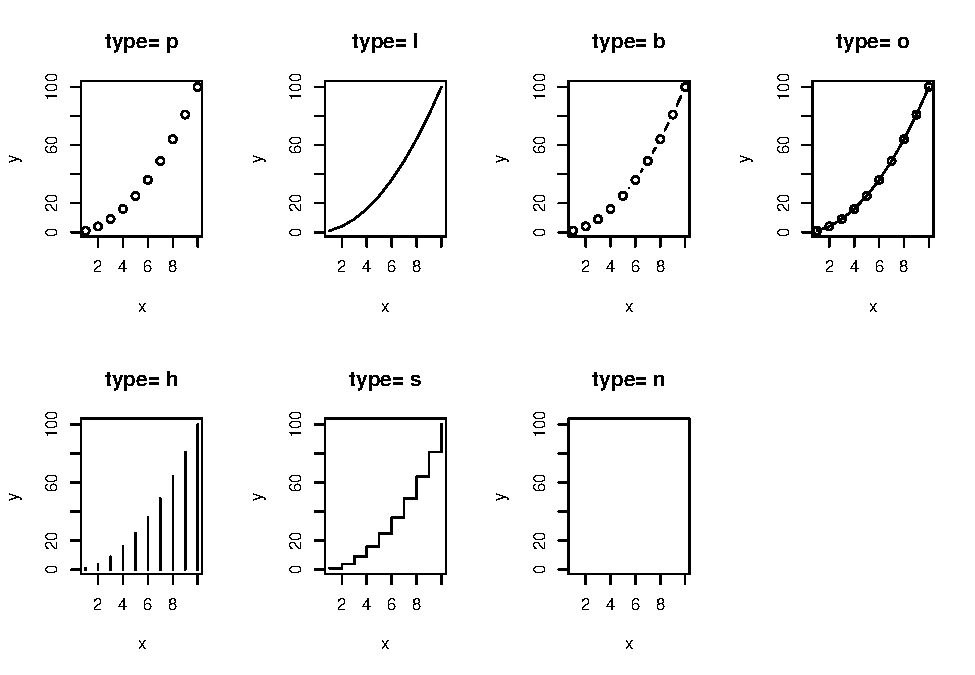
\includegraphics[width=0.8\linewidth]{Metode_Numerik_files/figure-latex/plot-1} 

}

\caption{Plot berbagai jenis setting type}\label{fig:plot}
\end{figure}

Pada contoh selanjutnya kita akan mencoba membuat kembali data yang akan kita plotkan. Data pada contoh kali ini merupakan data suatu fungsi matematika. Berikut adalah sintaks yang digunakan:

\begin{Shaded}
\begin{Highlighting}[]
\FunctionTok{set.seed}\NormalTok{(}\DecValTok{123}\NormalTok{)}
\NormalTok{x }\OtherTok{\textless{}{-}} \FunctionTok{seq}\NormalTok{(}\AttributeTok{from=}\DecValTok{0}\NormalTok{, }\AttributeTok{to=}\DecValTok{10}\NormalTok{, }\AttributeTok{by=}\FloatTok{0.1}\NormalTok{)}
\NormalTok{y }\OtherTok{\textless{}{-}}\NormalTok{ x}\SpecialCharTok{\^{}}\DecValTok{2}\SpecialCharTok{*}\FunctionTok{exp}\NormalTok{(}\SpecialCharTok{{-}}\NormalTok{x}\SpecialCharTok{/}\DecValTok{2}\NormalTok{)}\SpecialCharTok{*}\NormalTok{(}\DecValTok{1}\SpecialCharTok{+}\FunctionTok{rnorm}\NormalTok{(}\AttributeTok{n=}\FunctionTok{length}\NormalTok{(x), }\AttributeTok{mean=}\DecValTok{0}\NormalTok{, }\AttributeTok{sd=}\FloatTok{0.05}\NormalTok{))}
\end{Highlighting}
\end{Shaded}

\begin{Shaded}
\begin{Highlighting}[]
\FunctionTok{par}\NormalTok{(}\AttributeTok{mfrow=}\FunctionTok{c}\NormalTok{(}\DecValTok{1}\NormalTok{,}\DecValTok{2}\NormalTok{),}
    \CommentTok{\# mengatur margin grafik}
    \AttributeTok{mar=}\FunctionTok{c}\NormalTok{(}\DecValTok{4}\NormalTok{,}\DecValTok{4}\NormalTok{,}\FloatTok{1.5}\NormalTok{,}\FloatTok{1.5}\NormalTok{),}
    \CommentTok{\# mengatur margin sumbu}
    \AttributeTok{mex=}\FloatTok{0.8}\NormalTok{,}
    \CommentTok{\# arah tick sumbu koordinat}
    \AttributeTok{tcl=}\FloatTok{0.3}\NormalTok{)}
\FunctionTok{plot}\NormalTok{(x, y, }\AttributeTok{type=}\StringTok{"l"}\NormalTok{)}
\FunctionTok{plot}\NormalTok{(x, y, }\AttributeTok{type=}\StringTok{"o"}\NormalTok{)}
\end{Highlighting}
\end{Shaded}

\begin{figure}

{\centering 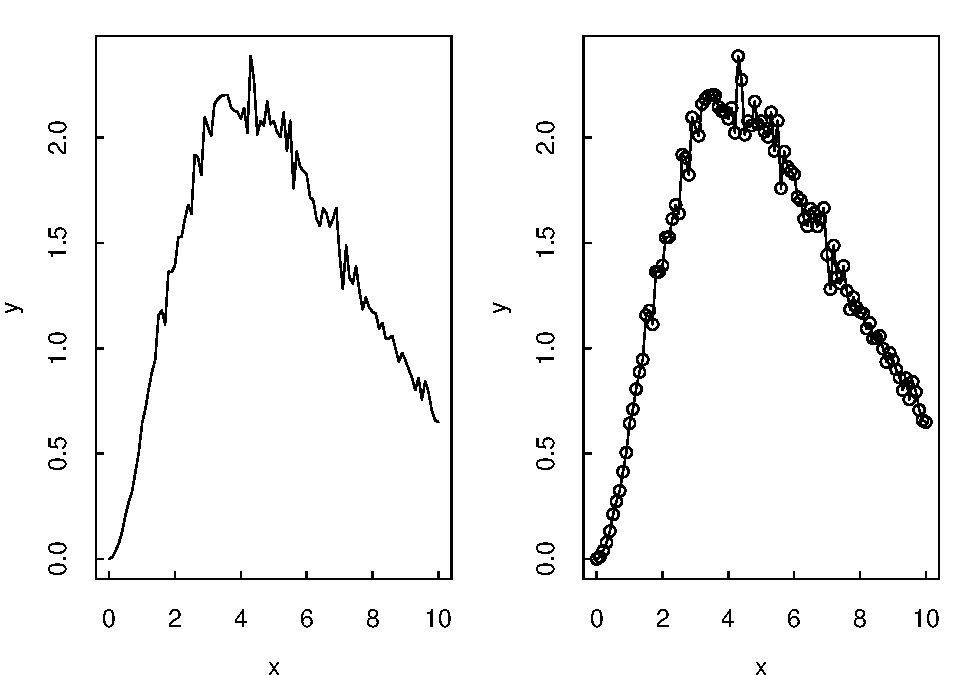
\includegraphics[width=0.8\linewidth]{Metode_Numerik_files/figure-latex/plot2-1} 

}

\caption{Plot fungsi matematika}\label{fig:plot2}
\end{figure}

Fungsi lain yang dapat digunakan untuk membuat kurva suatu persamaan matematis adalah fungsi \texttt{curve()}. Berbeda dengan fungsi \texttt{plot()} yang perlu menspesifikasi objek pada sumbu x dan y, fungsi \texttt{curve()} hanya perlu menspesifikasi objek sumbu x saja. Format fungsi \texttt{curve()} adalah sebagai berikut:

\begin{Shaded}
\begin{Highlighting}[]
\FunctionTok{curve}\NormalTok{(expr, }\AttributeTok{from =} \ConstantTok{NULL}\NormalTok{, }\AttributeTok{to =} \ConstantTok{NULL}\NormalTok{, }\AttributeTok{add =} \ConstantTok{FALSE}\NormalTok{)}
\end{Highlighting}
\end{Shaded}

\begin{quote}
\textbf{Catatan:}

\begin{itemize}
\tightlist
\item
  \textbf{expr}: persamaan matematika
\item
  \textbf{from dan to}: nilai awal dan akhir (maksimum atau minimum)
\item
  \textbf{add}: nilai logik yang menentukan apakah kurva perlu ditambahkan kedalam kurva sebelumnya.
\end{itemize}
\end{quote}

Berikut adalah contoh visualisasi menggunakan fungsi \texttt{curve()}:

\begin{Shaded}
\begin{Highlighting}[]
\FunctionTok{par}\NormalTok{(}\AttributeTok{mfrow=}\FunctionTok{c}\NormalTok{(}\DecValTok{1}\NormalTok{,}\DecValTok{2}\NormalTok{),}
    \CommentTok{\# mengatur margin grafik}
    \AttributeTok{mar=}\FunctionTok{c}\NormalTok{(}\DecValTok{4}\NormalTok{,}\DecValTok{4}\NormalTok{,}\FloatTok{1.5}\NormalTok{,}\FloatTok{1.5}\NormalTok{),}
    \CommentTok{\# mengatur margin sumbu}
    \AttributeTok{mex=}\FloatTok{0.8}\NormalTok{,}
    \CommentTok{\# arah tick sumbu koordinat}
    \AttributeTok{tcl=}\FloatTok{0.3}\NormalTok{)}

\CommentTok{\# Grafik kiri}
\FunctionTok{curve}\NormalTok{(}\AttributeTok{expr=}\NormalTok{x}\SpecialCharTok{\^{}}\DecValTok{2}\SpecialCharTok{*}\FunctionTok{exp}\NormalTok{(}\SpecialCharTok{{-}}\NormalTok{x}\SpecialCharTok{/}\DecValTok{2}\NormalTok{), }
      \AttributeTok{from=}\DecValTok{0}\NormalTok{, }\AttributeTok{to=}\DecValTok{10}\NormalTok{)}

\CommentTok{\# Grafik kanan}
\FunctionTok{plot}\NormalTok{(x, y, }\AttributeTok{pch=}\DecValTok{19}\NormalTok{, }\AttributeTok{cex=}\FloatTok{0.7}\NormalTok{,}
     \AttributeTok{xlab=}\StringTok{"Waktu (detik)"}\NormalTok{,}
     \AttributeTok{ylab=}\StringTok{"Sinyal Intensitas"}\NormalTok{)}
\FunctionTok{curve}\NormalTok{(}\AttributeTok{expr=}\NormalTok{x}\SpecialCharTok{\^{}}\DecValTok{2}\SpecialCharTok{*}\FunctionTok{exp}\NormalTok{(}\SpecialCharTok{{-}}\NormalTok{x}\SpecialCharTok{/}\DecValTok{2}\NormalTok{), }
      \AttributeTok{from=}\DecValTok{0}\NormalTok{, }\AttributeTok{to=}\DecValTok{10}\NormalTok{, }\AttributeTok{add=}\ConstantTok{TRUE}\NormalTok{)}
\end{Highlighting}
\end{Shaded}

\begin{figure}

{\centering 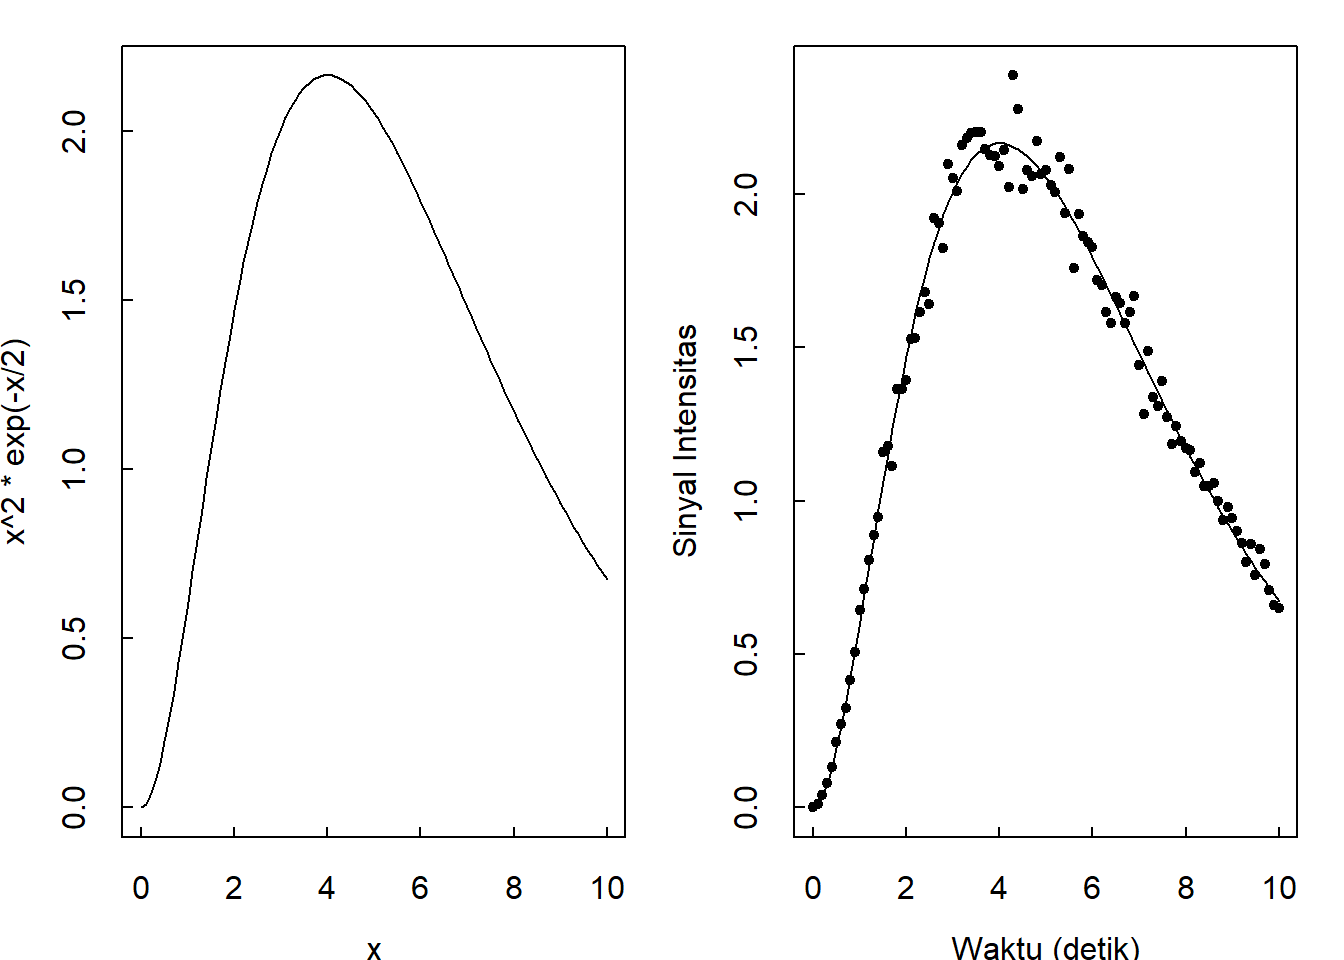
\includegraphics[width=0.8\linewidth]{Metode_Numerik_files/figure-latex/curve-1} 

}

\caption{Visualisasi menggunakan fungsi curve (sebelah kiri) dan visualisasi menggunakan fungsi plot dan curve (sebelah kanan)}\label{fig:curve}
\end{figure}

\hypertarget{otherviz}{%
\section{Visualisasi Lainnya}\label{otherviz}}

Visualisasi lainnya yang sering digunakan antara lain: histogram, density plot, bar plot, dan box plot.

\hypertarget{barplot}{%
\subsection{Bar Plot}\label{barplot}}

Barplot pada \texttt{R} dapat dibuat menggunakan fungsi \texttt{barplot()}. Untuk lebih memahaminya berikut disajikan contoh barplot menggunakan dataset \texttt{VADeaths}. Untuk memuatnya jalankan sintaks berikut:

\begin{Shaded}
\begin{Highlighting}[]
\NormalTok{VADeaths}
\end{Highlighting}
\end{Shaded}

\begin{verbatim}
##       Rural Male Rural Female Urban Male Urban Female
## 50-54       11.7          8.7       15.4          8.4
## 55-59       18.1         11.7       24.3         13.6
## 60-64       26.9         20.3       37.0         19.3
## 65-69       41.0         30.9       54.6         35.1
## 70-74       66.0         54.3       71.1         50.0
\end{verbatim}

Contoh bar plot untuk variabel \texttt{Rural\ Male} disajikan pada Gambar \ref{fig:barplot}:

\begin{Shaded}
\begin{Highlighting}[]
\FunctionTok{par}\NormalTok{(}\AttributeTok{mfrow=}\FunctionTok{c}\NormalTok{(}\DecValTok{1}\NormalTok{,}\DecValTok{2}\NormalTok{))}
\FunctionTok{barplot}\NormalTok{(VADeaths[, }\StringTok{"Rural Male"}\NormalTok{], }\AttributeTok{main=}\StringTok{"a"}\NormalTok{)}
\FunctionTok{barplot}\NormalTok{(VADeaths[, }\StringTok{"Rural Male"}\NormalTok{], }\AttributeTok{main=}\StringTok{"b"}\NormalTok{, }\AttributeTok{horiz=}\ConstantTok{TRUE}\NormalTok{)}
\end{Highlighting}
\end{Shaded}

\begin{figure}

{\centering 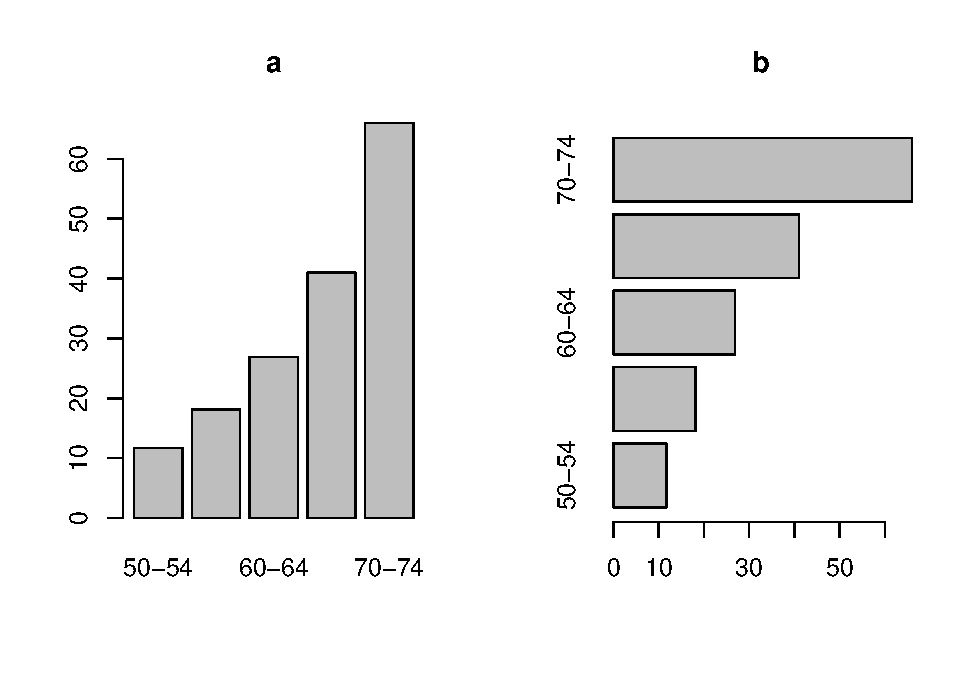
\includegraphics[width=0.7\linewidth]{Metode_Numerik_files/figure-latex/barplot-1} 

}

\caption{a. bar plot vertikal; b. bar plot horizontal}\label{fig:barplot}
\end{figure}

\begin{Shaded}
\begin{Highlighting}[]
\FunctionTok{par}\NormalTok{(}\AttributeTok{mfrow=}\FunctionTok{c}\NormalTok{(}\DecValTok{1}\NormalTok{,}\DecValTok{1}\NormalTok{))}
\end{Highlighting}
\end{Shaded}

Kita dapat mengubah warna pada masing-masing bar, baik outline bar maupun box pada bar. Selain itu kita juga dapat mengubah nama grup yang telah dihasilkan sebelumnya. Berikut sintaks untuk melakukannya dan output yang dihasilkan pada Gambar \ref{fig:barplot2}:

\begin{Shaded}
\begin{Highlighting}[]
\FunctionTok{barplot}\NormalTok{(VADeaths[, }\StringTok{"Rural Male"}\NormalTok{],}
        \CommentTok{\# ubah warna ouline menjadi steelblue}
        \AttributeTok{border=}\StringTok{"steelblue"}\NormalTok{,}
        \CommentTok{\# ubah wana box}
        \AttributeTok{col=} \FunctionTok{c}\NormalTok{(}\StringTok{"grey"}\NormalTok{, }\StringTok{"yellow"}\NormalTok{, }\StringTok{"steelblue"}\NormalTok{, }\StringTok{"green"}\NormalTok{, }\StringTok{"orange"}\NormalTok{),}
        \CommentTok{\# ubah nama grup dari A sampai E}
        \AttributeTok{names.arg =}\NormalTok{ LETTERS[}\DecValTok{1}\SpecialCharTok{:}\DecValTok{5}\NormalTok{],}
        \CommentTok{\# ubah orientasi menajadi horizontal}
        \AttributeTok{horiz=}\ConstantTok{TRUE}\NormalTok{)}
\end{Highlighting}
\end{Shaded}

\begin{figure}

{\centering 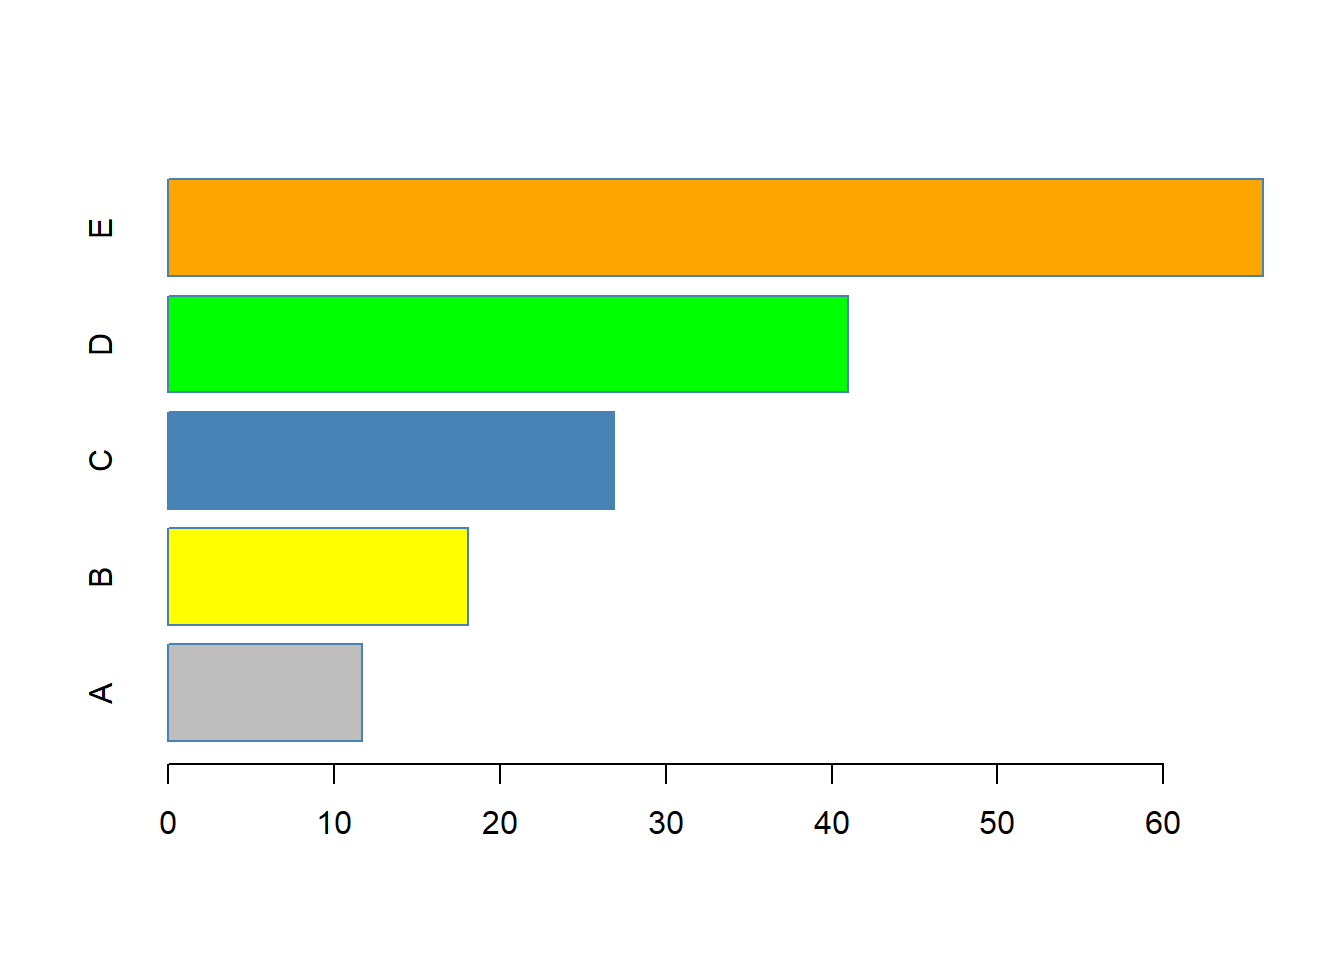
\includegraphics[width=0.7\linewidth]{Metode_Numerik_files/figure-latex/barplot2-1} 

}

\caption{Kustomisasi bar plot}\label{fig:barplot2}
\end{figure}

Untuk bar plot dengan \emph{multiple group}, tersedia dua pengaturan posisi yaitu \emph{stacked bar plot}(menunjukkan proporsi penyusun pada masing-masing grup) dan \emph{grouped bar plot}(melihat perbedaan individual pada masing-masing grup). Pada Gambar \ref{fig:barplot3} dan Gambar \ref{fig:barplot4} , disajikan kedua jenis bar plot tersebut.

\begin{Shaded}
\begin{Highlighting}[]
\CommentTok{\# staked}
\FunctionTok{barplot}\NormalTok{(VADeaths,}
         \AttributeTok{col =} \FunctionTok{c}\NormalTok{(}\StringTok{"lightblue"}\NormalTok{, }\StringTok{"mistyrose"}\NormalTok{, }\StringTok{"lightcyan"}\NormalTok{, }
                 \StringTok{"lavender"}\NormalTok{, }\StringTok{"cornsilk"}\NormalTok{),}
        \AttributeTok{legend =} \FunctionTok{rownames}\NormalTok{(VADeaths))}
\end{Highlighting}
\end{Shaded}

\begin{figure}

{\centering 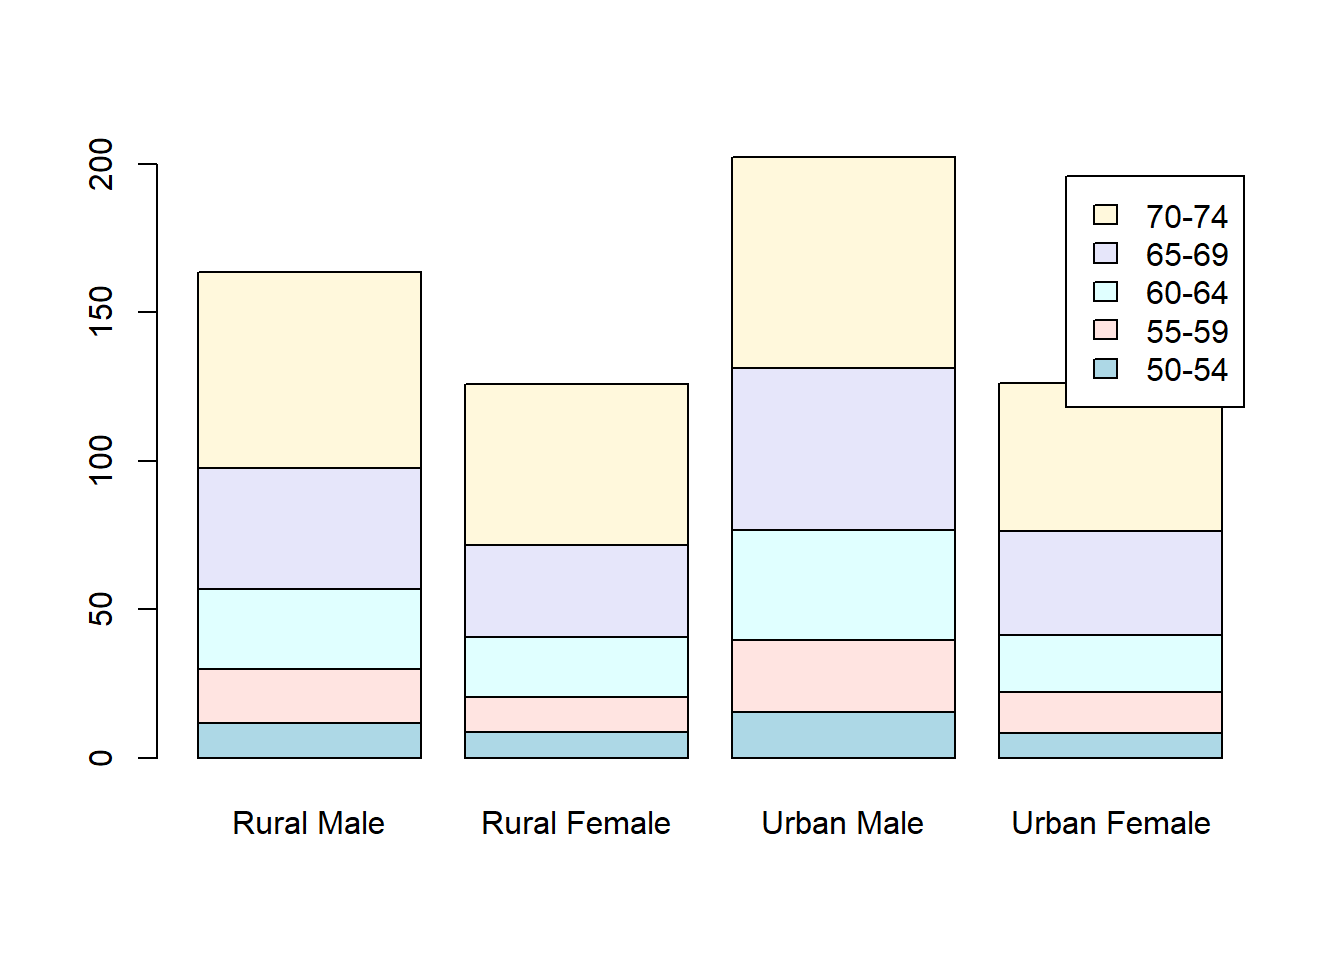
\includegraphics[width=0.7\linewidth]{Metode_Numerik_files/figure-latex/barplot3-1} 

}

\caption{Stacked bar plot}\label{fig:barplot3}
\end{figure}

\begin{Shaded}
\begin{Highlighting}[]
\CommentTok{\# grouped}
\FunctionTok{barplot}\NormalTok{(VADeaths,}
         \AttributeTok{col =} \FunctionTok{c}\NormalTok{(}\StringTok{"lightblue"}\NormalTok{, }\StringTok{"mistyrose"}\NormalTok{, }\StringTok{"lightcyan"}\NormalTok{, }
                 \StringTok{"lavender"}\NormalTok{, }\StringTok{"cornsilk"}\NormalTok{),}
        \AttributeTok{legend =} \FunctionTok{rownames}\NormalTok{(VADeaths), }\AttributeTok{beside =} \ConstantTok{TRUE}\NormalTok{)}
\end{Highlighting}
\end{Shaded}

\begin{figure}

{\centering 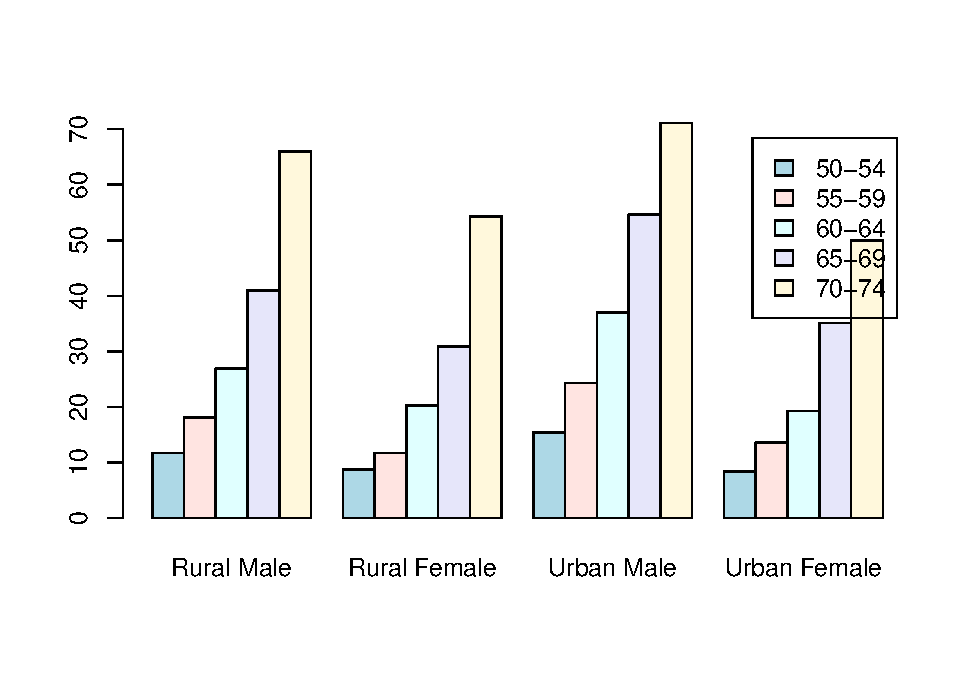
\includegraphics[width=0.7\linewidth]{Metode_Numerik_files/figure-latex/barplot4-1} 

}

\caption{Grouped bar plot}\label{fig:barplot4}
\end{figure}

\hypertarget{histogram}{%
\subsection{Histogram dan Density Plot}\label{histogram}}

Fungsi \texttt{hist()} dapat digunakan untuk membuat histogram pada \texttt{R}. Secara sederhana fungsi tersebut didefinisikan sebagai berikut:

\begin{Shaded}
\begin{Highlighting}[]
\FunctionTok{hist}\NormalTok{(x, }\AttributeTok{breaks=}\StringTok{"Sturges"}\NormalTok{)}
\end{Highlighting}
\end{Shaded}

\begin{quote}
\textbf{Catatan: }

\begin{itemize}
\tightlist
\item
  \textbf{x}: vektor numerik
\item
  \textbf{breaks}: \emph{breakpoints} antar sel histogram.
\end{itemize}
\end{quote}

Pada dataset \texttt{trees} akan dibuat histogram variabel \texttt{Height}. Untuk melakukannya jalankan sintaks berikut:

\begin{Shaded}
\begin{Highlighting}[]
\FunctionTok{hist}\NormalTok{(trees}\SpecialCharTok{$}\NormalTok{Height)}
\end{Highlighting}
\end{Shaded}

Output yang dihasilkan disajikan pada Gambar \ref{fig:hist}:

\begin{figure}

{\centering 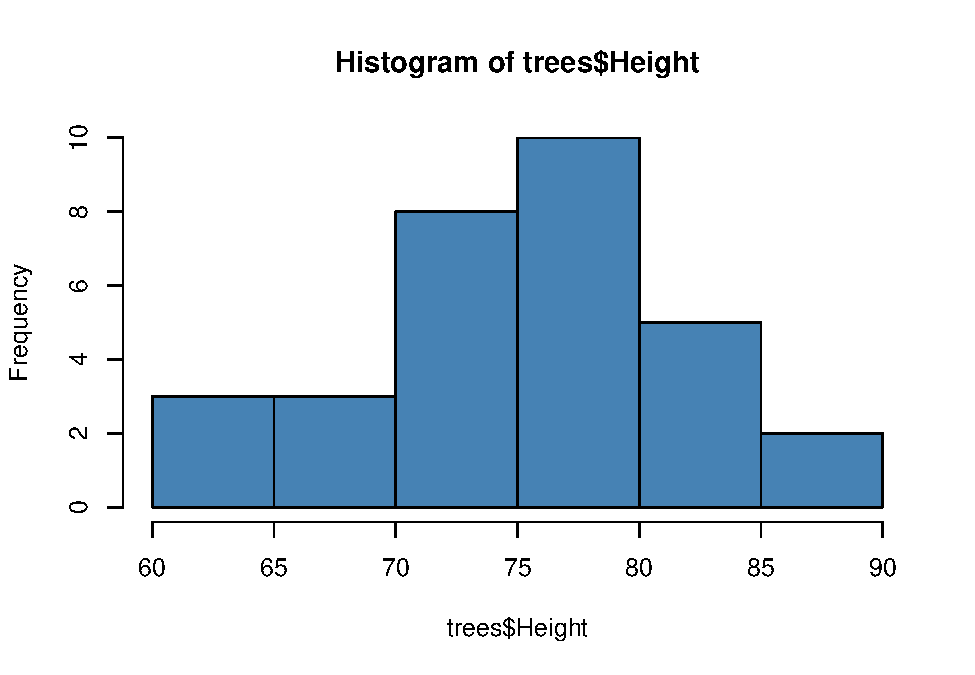
\includegraphics[width=0.7\linewidth]{Metode_Numerik_files/figure-latex/hist-1} 

}

\caption{Histogram}\label{fig:hist}
\end{figure}

Density plot pada \texttt{R} dapat dibuat menggunakan fungsi \texttt{density()}. Berbeda dengan fungsi \texttt{hist()}, fungsi ini tidak langsung menghasilkan grafik densitas. Fungsi \texttt{density()} hanya menghitung kernel densitas pada data. Densitas yang telah dihitung selanjutnya diplotkan menggunakan fungsi \texttt{plot()}. Berikut adalah sintaks dan output yang dihasilkan pada Gambar \ref{fig:dens}:

\begin{Shaded}
\begin{Highlighting}[]
\CommentTok{\# menghitung kernel density}
\NormalTok{dens }\OtherTok{\textless{}{-}} \FunctionTok{density}\NormalTok{(trees}\SpecialCharTok{$}\NormalTok{Height)}

\CommentTok{\# plot densitas dengan outline merah}
\FunctionTok{plot}\NormalTok{(dens,}\AttributeTok{col=}\StringTok{"red"}\NormalTok{)}
\end{Highlighting}
\end{Shaded}

\begin{figure}

{\centering 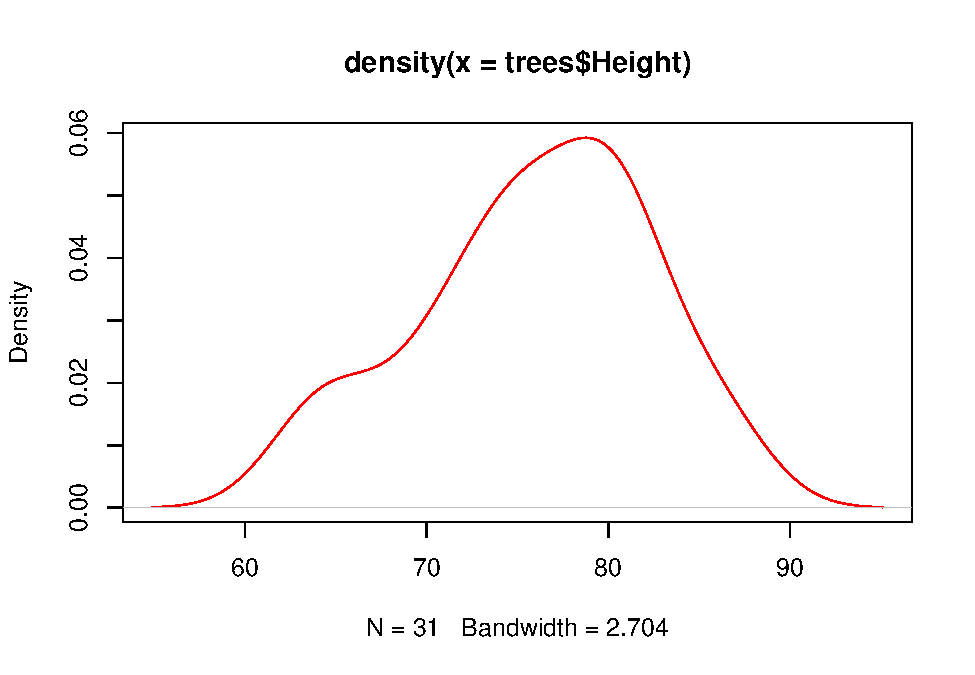
\includegraphics[width=0.7\linewidth]{Metode_Numerik_files/figure-latex/dens-1} 

}

\caption{Density plot}\label{fig:dens}
\end{figure}

Kita juga dapat menambahkan grafik densitas pada histogram sehingga mempermudah pembacaan pada histogram. Untuk melakukannya kita perlu mengubah kernel histigram dari frekuensi menjadi density dengan menambahkan argumen \texttt{freq=FALSE} pada fungsi \texttt{hist()}. Selanjutnya tambahkan fungsi \texttt{polygon()} untuk memplotkan grafik densitas. Berikut adalah sintak dan output yang dihasilkan pada Gambar \ref{fig:denshist}:

\begin{Shaded}
\begin{Highlighting}[]
\CommentTok{\# menghitung kernel density}
\NormalTok{dens }\OtherTok{\textless{}{-}} \FunctionTok{density}\NormalTok{(trees}\SpecialCharTok{$}\NormalTok{Height)}

\CommentTok{\# histogram}
\FunctionTok{hist}\NormalTok{(trees}\SpecialCharTok{$}\NormalTok{Height, }\AttributeTok{freq=}\ConstantTok{FALSE}\NormalTok{, }\AttributeTok{col=}\StringTok{"steelblue"}\NormalTok{)}

\CommentTok{\# tambahkan density plot}
\FunctionTok{polygon}\NormalTok{(dens, }\AttributeTok{border=}\StringTok{"red"}\NormalTok{)}
\end{Highlighting}
\end{Shaded}

\begin{figure}

{\centering 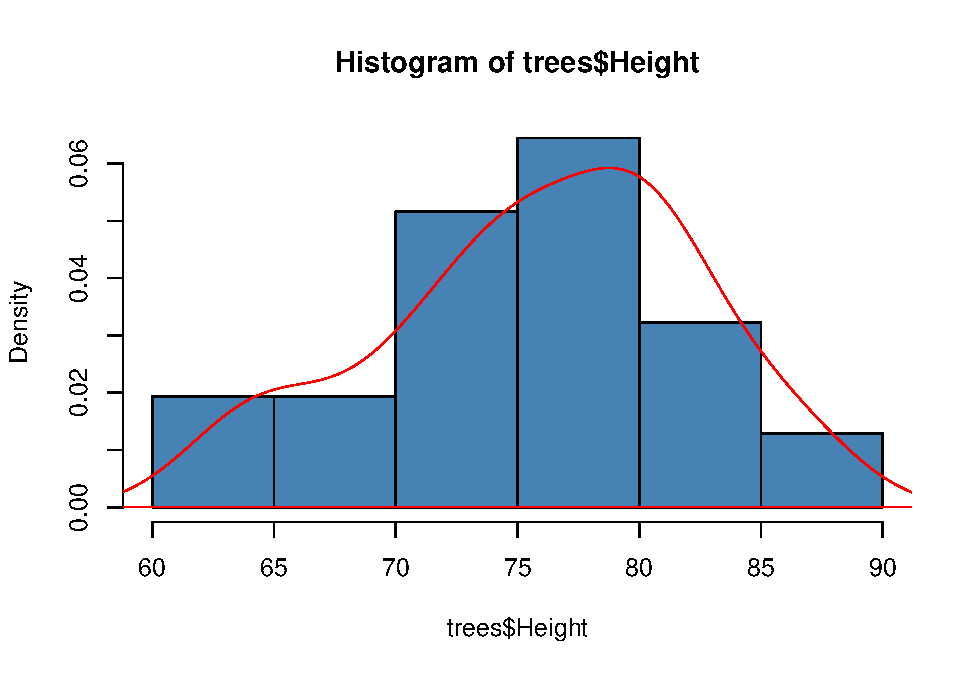
\includegraphics[width=0.7\linewidth]{Metode_Numerik_files/figure-latex/denshist-1} 

}

\caption{Density plot dan histogram}\label{fig:denshist}
\end{figure}

\hypertarget{boxplot}{%
\subsection{Box plot}\label{boxplot}}

Box plot pada \texttt{R} dapat dibuat menggunakan fungsi \texttt{boxplot()}. Berikut adalah sintaks untuk membuat boxplot variabel \texttt{Sepal.Lenght} pada dataset \texttt{iris} dan output yang dihasilkan pada Gambar \ref{fig:boxplot}:

\begin{Shaded}
\begin{Highlighting}[]
\FunctionTok{boxplot}\NormalTok{(iris}\SpecialCharTok{$}\NormalTok{Sepal.Length)}
\end{Highlighting}
\end{Shaded}

\begin{figure}

{\centering 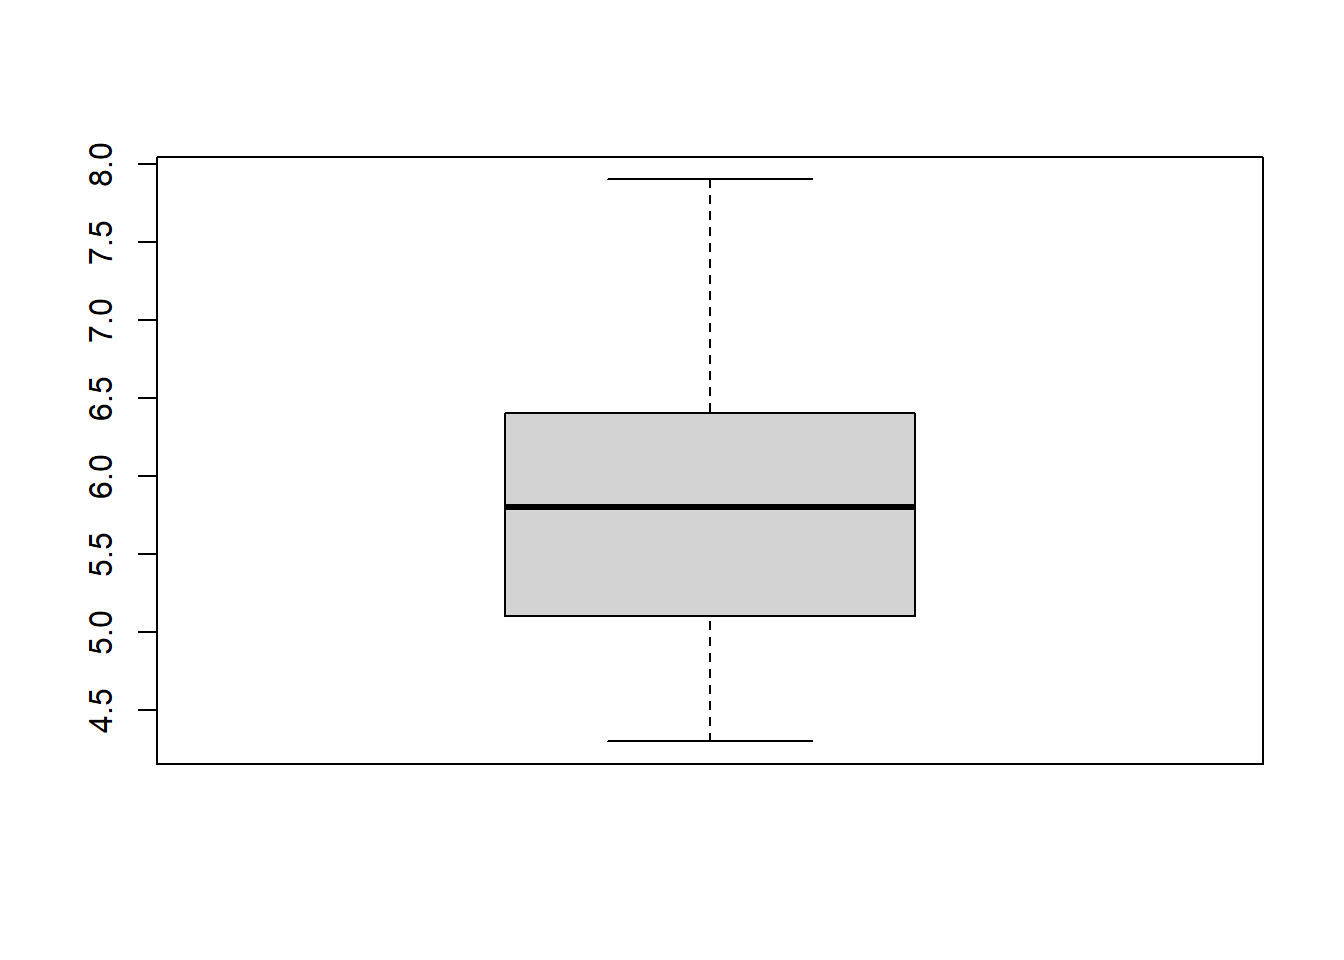
\includegraphics[width=0.7\linewidth]{Metode_Numerik_files/figure-latex/boxplot-1} 

}

\caption{Boxplot variabel Sepal.Length}\label{fig:boxplot}
\end{figure}

Boxplot juga dapat dibuat berdasarkan variabel factor. Hal ini berguna untuk melihat perbedaan ditribusi data pada masing-masing grup. Pada sintaks berikut dibuat boxplot berdasarkan variabel \texttt{Species}. Output yang dihasilkan disajikan pada Gambar \ref{fig:boxplot2}:

\begin{Shaded}
\begin{Highlighting}[]
\FunctionTok{boxplot}\NormalTok{(iris}\SpecialCharTok{$}\NormalTok{Sepal.Length}\SpecialCharTok{\textasciitilde{}}\NormalTok{iris}\SpecialCharTok{$}\NormalTok{Species)}
\end{Highlighting}
\end{Shaded}

\begin{figure}

{\centering 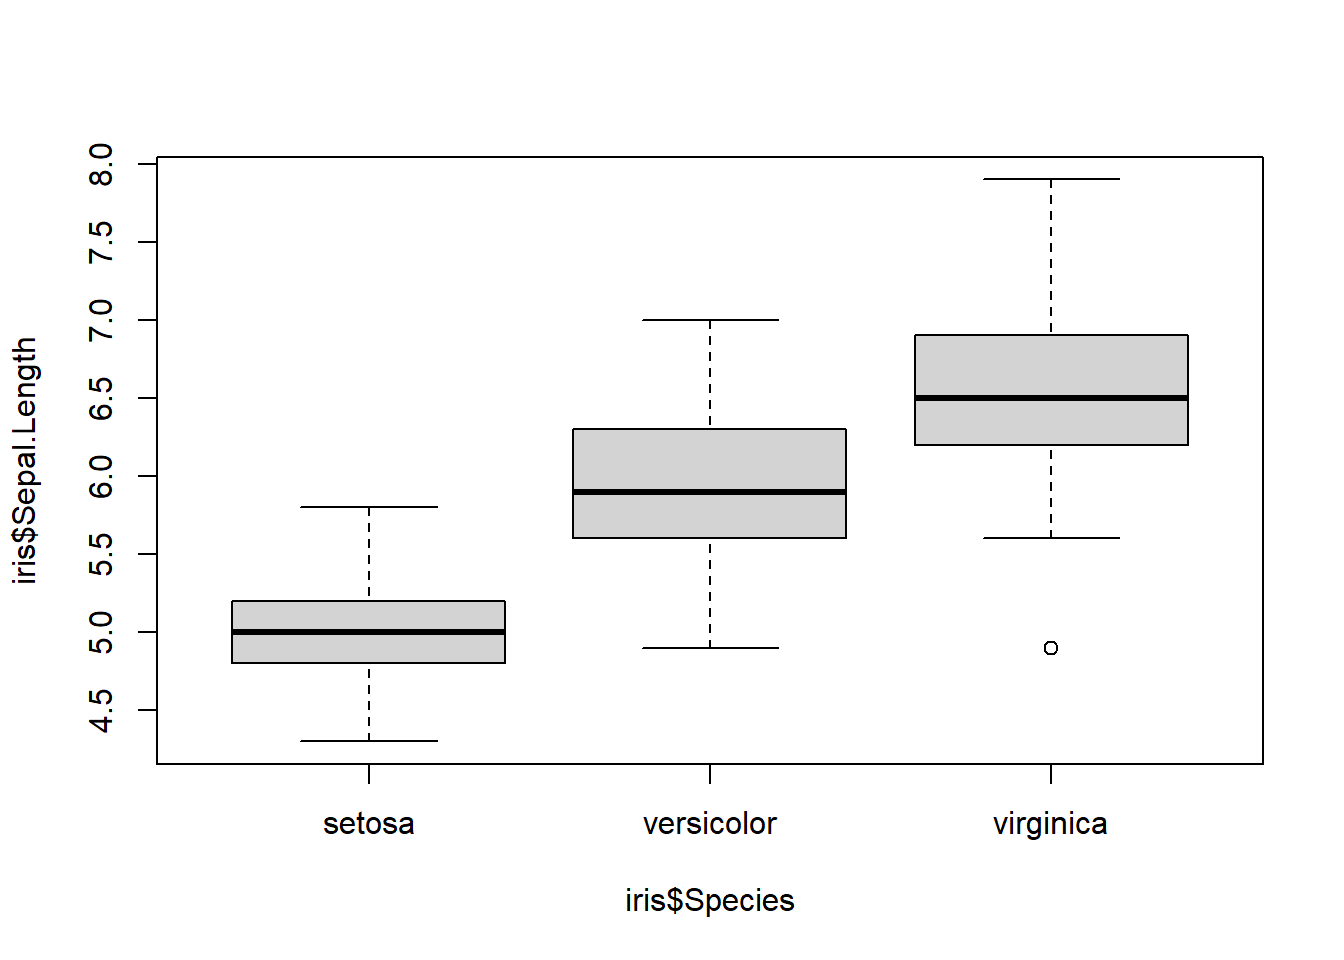
\includegraphics[width=0.7\linewidth]{Metode_Numerik_files/figure-latex/boxplot2-1} 

}

\caption{Boxplot berdasarkan variabel species}\label{fig:boxplot2}
\end{figure}

Kita juga dapat mengubah warna outline dan box pada boxplot. Berikut adalah contoh sintaks yang digunakan untuk melakukannya dan output yang dihasilkan disajikan pada Gambar \ref{fig:boxplot3}:

\begin{Shaded}
\begin{Highlighting}[]
\FunctionTok{boxplot}\NormalTok{(iris}\SpecialCharTok{$}\NormalTok{Sepal.Length}\SpecialCharTok{\textasciitilde{}}\NormalTok{iris}\SpecialCharTok{$}\NormalTok{Species,}
        \CommentTok{\# ubah warna outline menjadi steelblue}
        \AttributeTok{border =} \StringTok{"steelblue"}\NormalTok{,}
        \CommentTok{\# ubah warna box berdasarkan grup}
        \AttributeTok{col=} \FunctionTok{c}\NormalTok{(}\StringTok{"\#999999"}\NormalTok{, }\StringTok{"\#E69F00"}\NormalTok{, }\StringTok{"\#56B4E9"}\NormalTok{))}
\end{Highlighting}
\end{Shaded}

\begin{figure}

{\centering 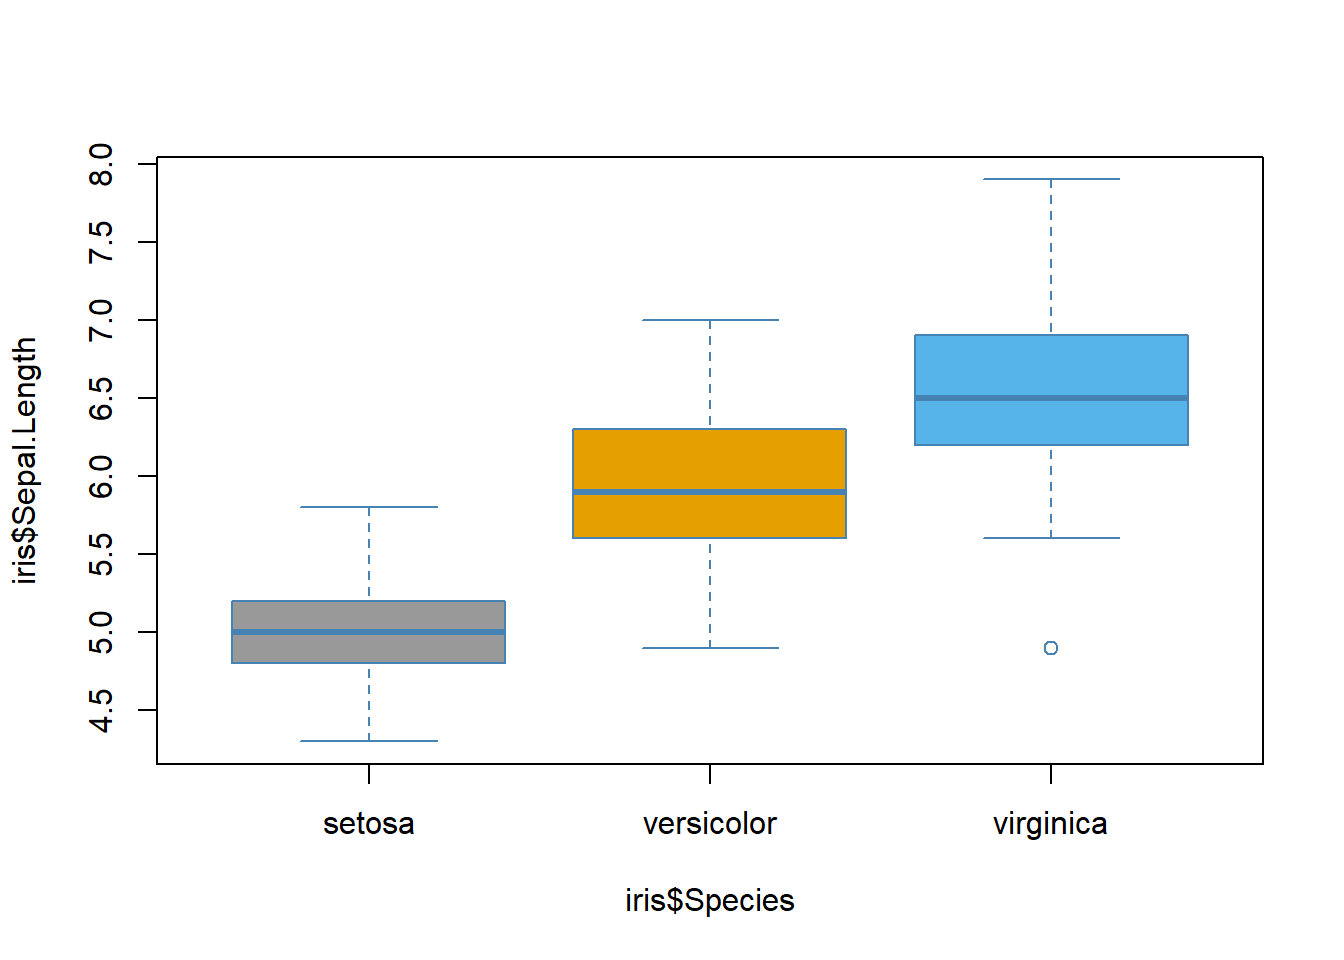
\includegraphics[width=0.7\linewidth]{Metode_Numerik_files/figure-latex/boxplot3-1} 

}

\caption{Boxplot dengan warna berdasarkan spesies}\label{fig:boxplot3}
\end{figure}

Kita juga dapat membuat boxplot pada \emph{multiple group}. Data yang digunakan untuk contoh tersebut adalah dataset \texttt{ToothGrowth}. Berikut adalah sintaks untuk memuat dataset tersebut:

\begin{Shaded}
\begin{Highlighting}[]
\CommentTok{\# ubah variable dose menjadi factor}
\NormalTok{ToothGrowth}\SpecialCharTok{$}\NormalTok{dose }\OtherTok{\textless{}{-}} \FunctionTok{as.factor}\NormalTok{(ToothGrowth}\SpecialCharTok{$}\NormalTok{dose)}

\CommentTok{\# print}
\FunctionTok{head}\NormalTok{(ToothGrowth)}
\end{Highlighting}
\end{Shaded}

\begin{verbatim}
##    len supp dose
## 1  4.2   VC  0.5
## 2 11.5   VC  0.5
## 3  7.3   VC  0.5
## 4  5.8   VC  0.5
## 5  6.4   VC  0.5
## 6 10.0   VC  0.5
\end{verbatim}

Contoh sintaks dan output boxplot \emph{multiple group} disajikan pada Gambar \ref{fig:boxplot4}:

\begin{Shaded}
\begin{Highlighting}[]
\FunctionTok{boxplot}\NormalTok{(len }\SpecialCharTok{\textasciitilde{}}\NormalTok{ supp}\SpecialCharTok{*}\NormalTok{dose, }\AttributeTok{data =}\NormalTok{ ToothGrowth,}
        \AttributeTok{col =} \FunctionTok{c}\NormalTok{(}\StringTok{"white"}\NormalTok{, }\StringTok{"steelblue"}\NormalTok{))}
\end{Highlighting}
\end{Shaded}

\begin{figure}

{\centering 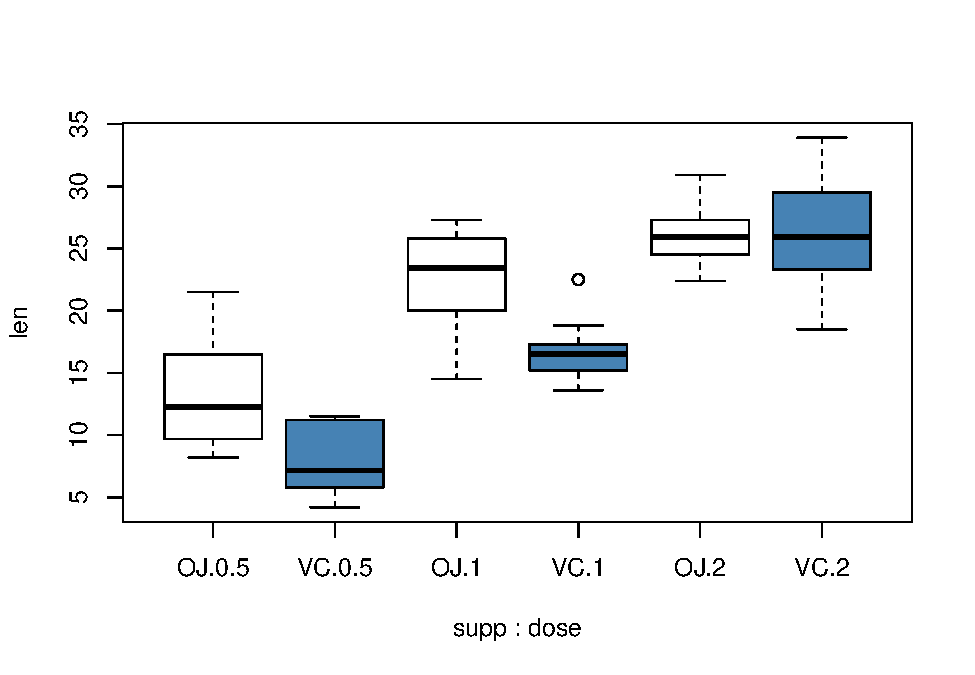
\includegraphics[width=0.7\linewidth]{Metode_Numerik_files/figure-latex/boxplot4-1} 

}

\caption{Boxplot multiple group}\label{fig:boxplot4}
\end{figure}

\hypertarget{customise}{%
\section{Kustomisasi Parameter Grafik}\label{customise}}

Pada bagian ini penulis akan menjelaskan cara untuk kustomisasi parameter grafik seperti:

\begin{enumerate}
\def\labelenumi{\alph{enumi}.}
\tightlist
\item
  menambahkan judul, legend, teks, axis, dan garis.
\item
  mengubah skala axis, simbol plot, jenis garis, dan warna.
\end{enumerate}

\hypertarget{addtitle}{%
\subsection{Menambahkan Judul}\label{addtitle}}

Pada grafik di \texttt{R}, kita dapat menambahkan judul dengan dua cara, yaitu: pada plot melalui parameter dan melalui fungsi plot(). Kedua cara tersebut tidak berbeda satu sama lain pada parameter input.

Untuk menambahkan judul pada plot secara langsung, kita dapat menggunakan argumen tambahan sebagai berikut:

\begin{enumerate}
\def\labelenumi{\alph{enumi}.}
\tightlist
\item
  \textbf{main}: teks untuk judul.
\item
  \textbf{xlab}: teks untuk keterangan axis X.
\item
  \textbf{ylab}: teks untuk keterangan axis y.
\item
  \textbf{sub}: teks untuk sub-judul.
\end{enumerate}

Berikut contoh sintaks penerapan masing-masing argumen tersebut beserta dengan output yang dihasilkan pada Gambar \ref{fig:title}:

\begin{Shaded}
\begin{Highlighting}[]
\CommentTok{\# menambahkan judul}
\FunctionTok{barplot}\NormalTok{(}\FunctionTok{c}\NormalTok{(}\DecValTok{2}\NormalTok{,}\DecValTok{5}\NormalTok{), }\AttributeTok{main=}\StringTok{"Main title"}\NormalTok{,}
        \AttributeTok{xlab=}\StringTok{"X axis title"}\NormalTok{,}
        \AttributeTok{ylab=}\StringTok{"Y axis title"}\NormalTok{,}
        \AttributeTok{sub=}\StringTok{"Sub{-}title"}\NormalTok{)}
\end{Highlighting}
\end{Shaded}

\begin{figure}

{\centering 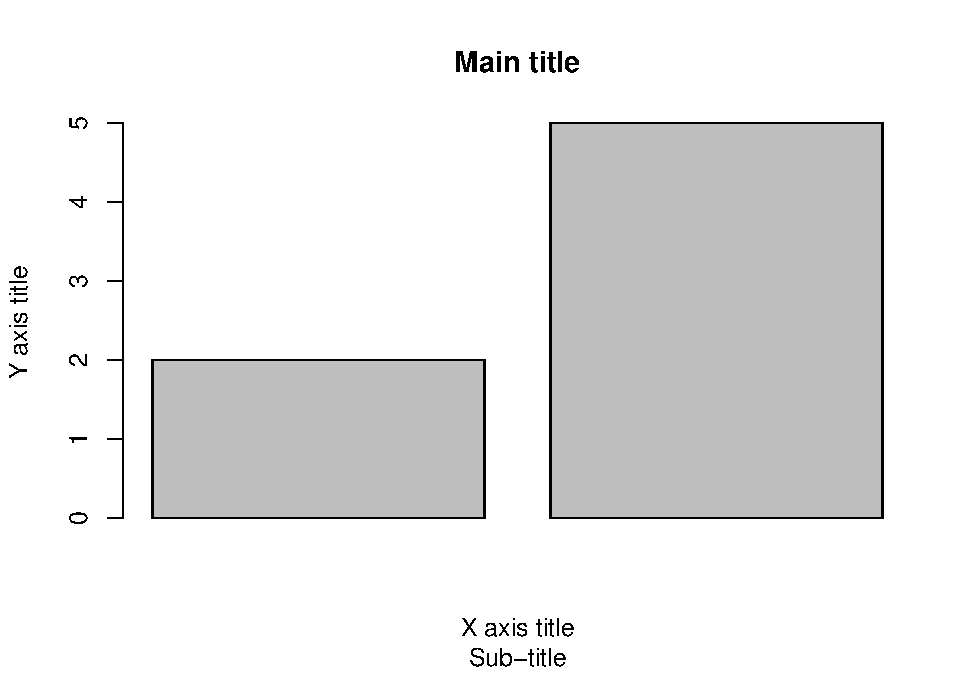
\includegraphics[width=0.7\linewidth]{Metode_Numerik_files/figure-latex/title-1} 

}

\caption{Menambahkan Judul}\label{fig:title}
\end{figure}

kita juga dapat melakukan kustomisasi pada warna, \emph{font style}, dan ukuran font judul. Untuk melakukan kustomisasi pada warna pada judul, kita dapat menambahkan argumen sebagai berikut:

\begin{enumerate}
\def\labelenumi{\alph{enumi}.}
\tightlist
\item
  \textbf{col.main}: warna untuk judul.
\item
  \textbf{col.lab}: warna untuk keterangan axis.
\item
  \textbf{col.sub}: warna untuk sub-judul
\end{enumerate}

Untuk kustomisasi font judul, kita dapat menambahkan argumen berikut:

\begin{enumerate}
\def\labelenumi{\alph{enumi}.}
\tightlist
\item
  \textbf{font.main}: \emph{font style} untuk judul.
\item
  \textbf{font.lab}: \emph{font style} untuk keterangan axis.
\item
  \textbf{font.sub}: \emph{font style} untuk sub-judul.
\end{enumerate}

\begin{quote}
\textbf{Penting!!!}

Nilai yang dapat dimasukkan antara lain:

\begin{itemize}
\tightlist
\item
  \textbf{1}: untuk teks normal.
\item
  \textbf{2}: untuk teks cetak tebal.
\item
  \textbf{3}: untuk teks cetak miring.
\item
  \textbf{4}: untuk teks cetak tebal dan miring.
\item
  \textbf{5}: untuk font simbol.
\end{itemize}
\end{quote}

Sedangkan untuk ukuran font, kita dapat menambahkan variabel berikut:

\begin{enumerate}
\def\labelenumi{\alph{enumi}.}
\tightlist
\item
  \textbf{cex.main}: ukuran teks judul.
\item
  \textbf{cex.lab}: ukuran teks keterangan axis.
\item
  \textbf{cex.sub}: ukuran teks sub-judul.
\end{enumerate}

Berikut sintaks penerapan seluruh argumen tersebut beserta output yang dihasilkan pada Gambar \ref{fig:title2}:

\begin{Shaded}
\begin{Highlighting}[]
\CommentTok{\# menambahkan judul}
\FunctionTok{barplot}\NormalTok{(}\FunctionTok{c}\NormalTok{(}\DecValTok{2}\NormalTok{,}\DecValTok{5}\NormalTok{), }
        \CommentTok{\# menambahkan judul}
        \AttributeTok{main=}\StringTok{"Main title"}\NormalTok{,}
        \AttributeTok{xlab=}\StringTok{"X axis title"}\NormalTok{,}
        \AttributeTok{ylab=}\StringTok{"Y axis title"}\NormalTok{,}
        \AttributeTok{sub=}\StringTok{"Sub{-}title"}\NormalTok{,}
        \CommentTok{\# kustomisasi warna font}
        \AttributeTok{col.main=}\StringTok{"red"}\NormalTok{, }
        \AttributeTok{col.lab=}\StringTok{"blue"}\NormalTok{, }
        \AttributeTok{col.sub=}\StringTok{"black"}\NormalTok{,}
        \CommentTok{\# kustomisasi font style}
        \AttributeTok{font.main=}\DecValTok{4}\NormalTok{, }
        \AttributeTok{font.lab=}\DecValTok{4}\NormalTok{, }
        \AttributeTok{font.sub=}\DecValTok{4}\NormalTok{,}
        \CommentTok{\# kustomisasi ukuran font}
        \AttributeTok{cex.main=}\DecValTok{2}\NormalTok{, }
        \AttributeTok{cex.lab=}\FloatTok{1.7}\NormalTok{, }
        \AttributeTok{cex.sub=}\FloatTok{1.2}\NormalTok{)}
\end{Highlighting}
\end{Shaded}

\begin{figure}

{\centering 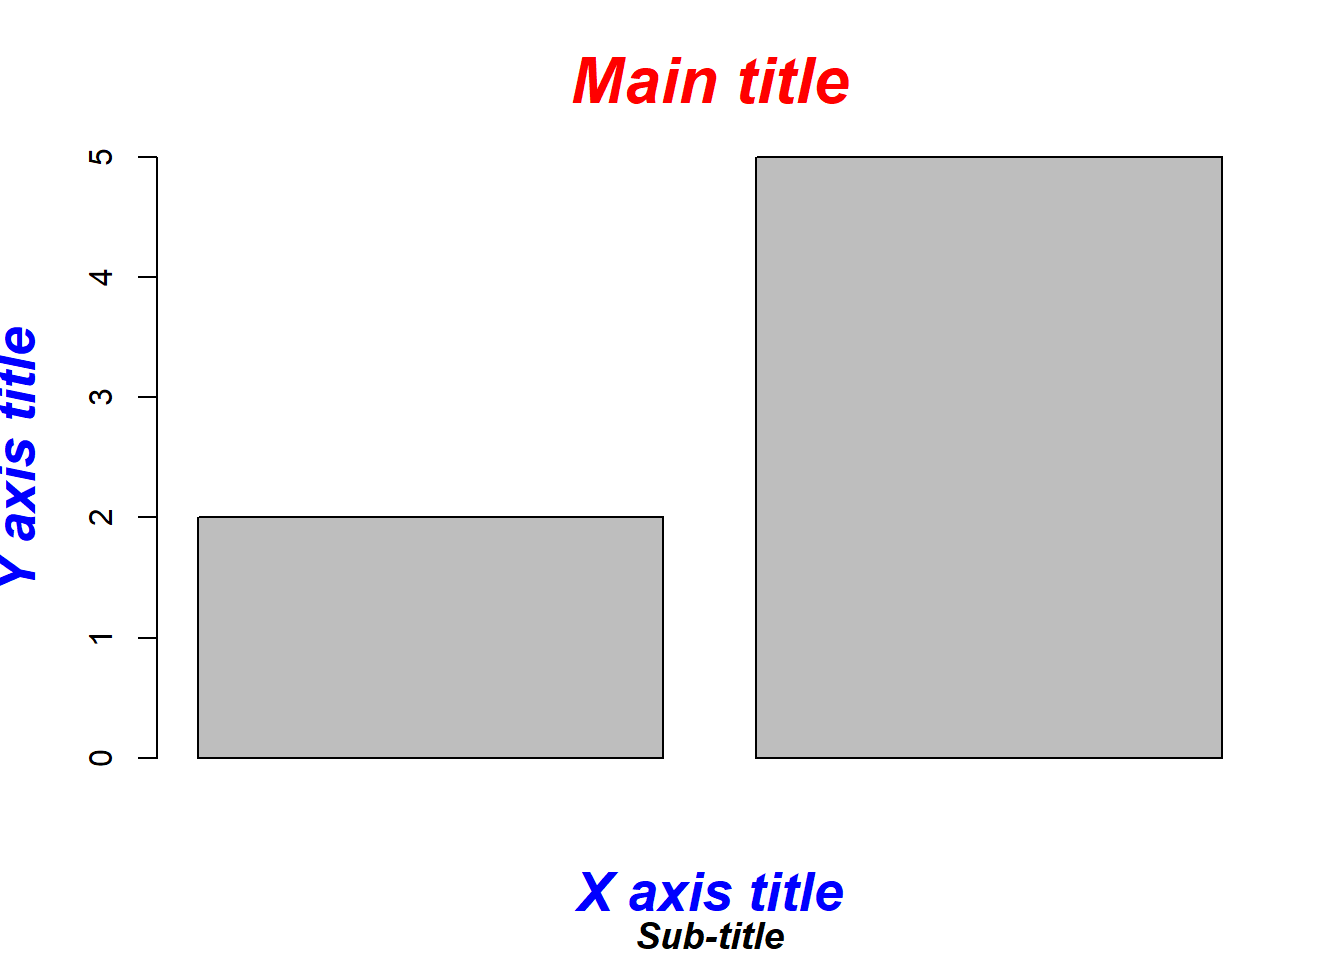
\includegraphics[width=0.7\linewidth]{Metode_Numerik_files/figure-latex/title2-1} 

}

\caption{Menambahkan Judul (2)}\label{fig:title2}
\end{figure}

Kita telah belajar bagaimana menambahkan judul langsung pada fungsi plot. Selain cara tersebut, telah penulis jelaskan bahwa kita dapat menambahkan judul melalui fungsi \texttt{title()}. argumen yang dimasukkan pada dasarnya tidak berbeda dengan ketika kita menambahkan judul secara langsung pada plot. Berikut adalah contoh sintaks dan output yang dihasilkan pada Gambar \ref{fig:title3}:

\begin{Shaded}
\begin{Highlighting}[]
\CommentTok{\# menambahkan judul}
\FunctionTok{barplot}\NormalTok{(}\FunctionTok{c}\NormalTok{(}\DecValTok{2}\NormalTok{,}\DecValTok{5}\NormalTok{,}\DecValTok{8}\NormalTok{))}

\CommentTok{\# menambahkan judul}
\FunctionTok{title}\NormalTok{(}\AttributeTok{main=}\StringTok{"Main title"}\NormalTok{,}
      \AttributeTok{xlab=}\StringTok{"X axis title"}\NormalTok{,}
      \AttributeTok{ylab=}\StringTok{"Y axis title"}\NormalTok{,}
      \AttributeTok{sub=}\StringTok{"Sub{-}title"}\NormalTok{,}
      \CommentTok{\# kustomisasi warna font}
      \AttributeTok{col.main=}\StringTok{"red"}\NormalTok{, }
      \AttributeTok{col.lab=}\StringTok{"blue"}\NormalTok{, }
      \AttributeTok{col.sub=}\StringTok{"black"}\NormalTok{,}
      \CommentTok{\# kustomisasi font style}
      \AttributeTok{font.main=}\DecValTok{4}\NormalTok{, }
      \AttributeTok{font.lab=}\DecValTok{4}\NormalTok{, }
      \AttributeTok{font.sub=}\DecValTok{4}\NormalTok{,}
      \CommentTok{\# kustomisasi ukuran font}
      \AttributeTok{cex.main=}\DecValTok{2}\NormalTok{, }
      \AttributeTok{cex.lab=}\FloatTok{1.7}\NormalTok{, }
      \AttributeTok{cex.sub=}\FloatTok{1.2}\NormalTok{)}
\end{Highlighting}
\end{Shaded}

\begin{figure}

{\centering 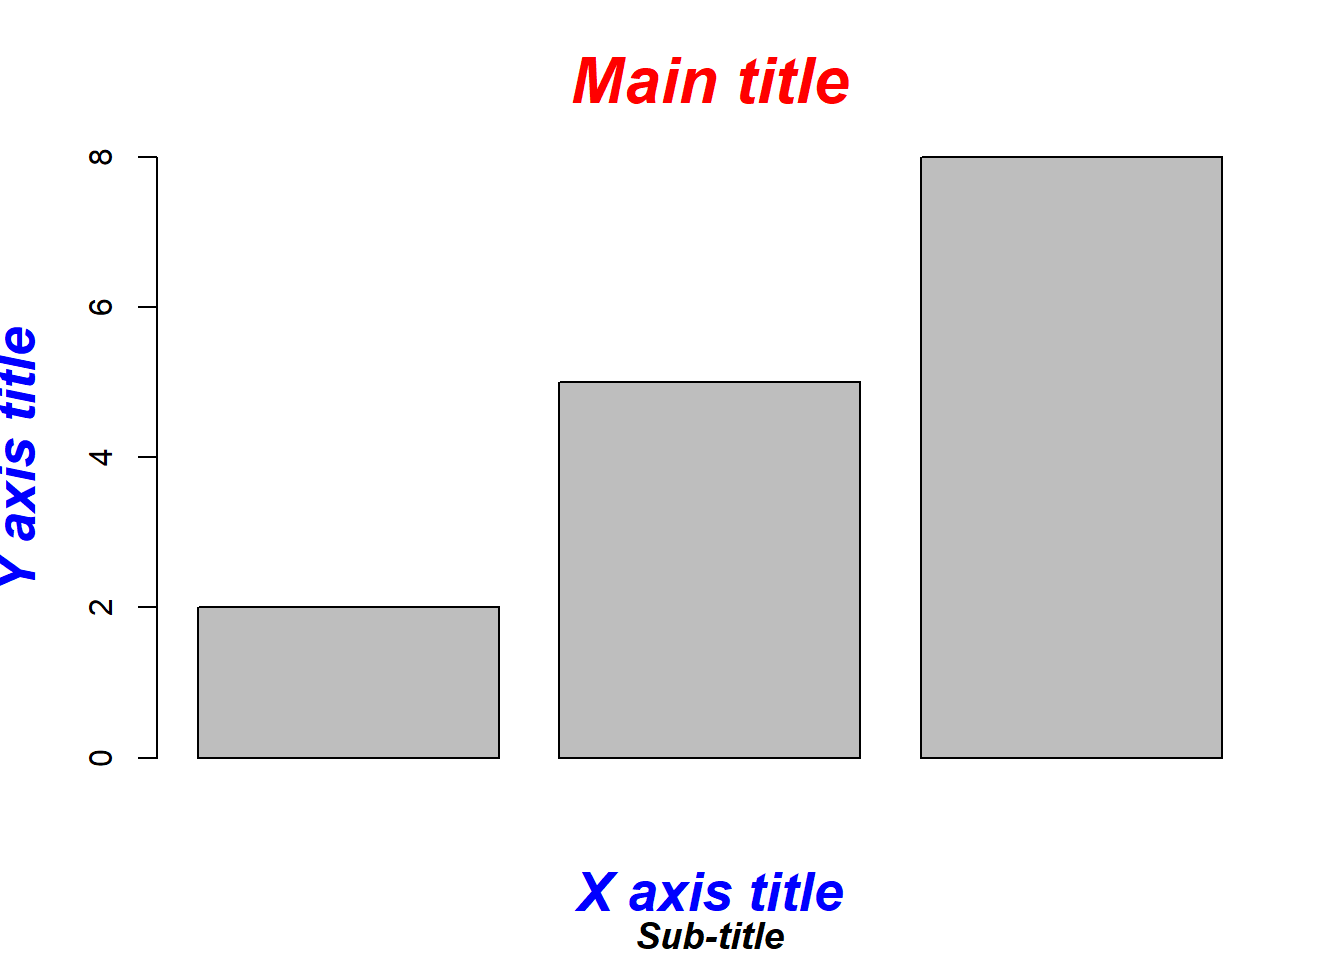
\includegraphics[width=0.7\linewidth]{Metode_Numerik_files/figure-latex/title3-1} 

}

\caption{Menambahkan Judul (3)}\label{fig:title3}
\end{figure}

\hypertarget{addlegend}{%
\subsection{Menambahkan Legend}\label{addlegend}}

Fungsi \texttt{legend()} pada \texttt{R} dapat digunakan untuk menambahkan legend pada grafik. Format sederhananya adalah sebagai berikut:

\begin{Shaded}
\begin{Highlighting}[]
\FunctionTok{legend}\NormalTok{(x, }\AttributeTok{y=}\ConstantTok{NULL}\NormalTok{, legend, fill, col, bg)}
\end{Highlighting}
\end{Shaded}

\begin{quote}
\textbf{Catatan:}

\begin{itemize}
\tightlist
\item
  \textbf{x} dan \textbf{y}: koordinat yang digunakan untuk posisi legend.
\item
  \textbf{legend}: teks pada legend
\item
  \textbf{fill}: warna yang digunakan untuk mengisi box disamping teks legend.
\item
  \textbf{col}: warna garis dan titik disamping teks legend.
\item
  \textbf{bg}: warna latar belakang legend box.
\end{itemize}
\end{quote}

Berikut adalah contoh sintaks dan ouput penerapan argumen disajikan pada Gambar \ref{fig:legend}:

\begin{Shaded}
\begin{Highlighting}[]
\CommentTok{\# membuat vektor numerik}
\NormalTok{x }\OtherTok{\textless{}{-}} \FunctionTok{c}\NormalTok{(}\DecValTok{1}\SpecialCharTok{:}\DecValTok{10}\NormalTok{)}
\NormalTok{y }\OtherTok{\textless{}{-}}\NormalTok{ x}\SpecialCharTok{\^{}}\DecValTok{2}
\NormalTok{z }\OtherTok{\textless{}{-}}\NormalTok{ x}\SpecialCharTok{*}\DecValTok{2}

\CommentTok{\# membuat line plot}
\FunctionTok{plot}\NormalTok{(x,y, }\AttributeTok{type=}\StringTok{"o"}\NormalTok{, }\AttributeTok{col=}\StringTok{"red"}\NormalTok{, }\AttributeTok{lty=}\DecValTok{1}\NormalTok{)}

\CommentTok{\# menambahkan line plot}
\FunctionTok{lines}\NormalTok{(x,z, }\AttributeTok{type=}\StringTok{"o"}\NormalTok{, }\AttributeTok{col=}\StringTok{"blue"}\NormalTok{, }\AttributeTok{lty=}\DecValTok{2}\NormalTok{)}

\CommentTok{\# menambahkan legend}
\FunctionTok{legend}\NormalTok{(}\DecValTok{1}\NormalTok{, }\DecValTok{95}\NormalTok{, }\AttributeTok{legend=}\FunctionTok{c}\NormalTok{(}\StringTok{"Line 1"}\NormalTok{, }\StringTok{"Line 2"}\NormalTok{),}
       \AttributeTok{col=}\FunctionTok{c}\NormalTok{(}\StringTok{"red"}\NormalTok{, }\StringTok{"blue"}\NormalTok{), }\AttributeTok{lty=}\DecValTok{1}\SpecialCharTok{:}\DecValTok{2}\NormalTok{, }\AttributeTok{cex=}\FloatTok{0.8}\NormalTok{)}
\end{Highlighting}
\end{Shaded}

\begin{figure}

{\centering 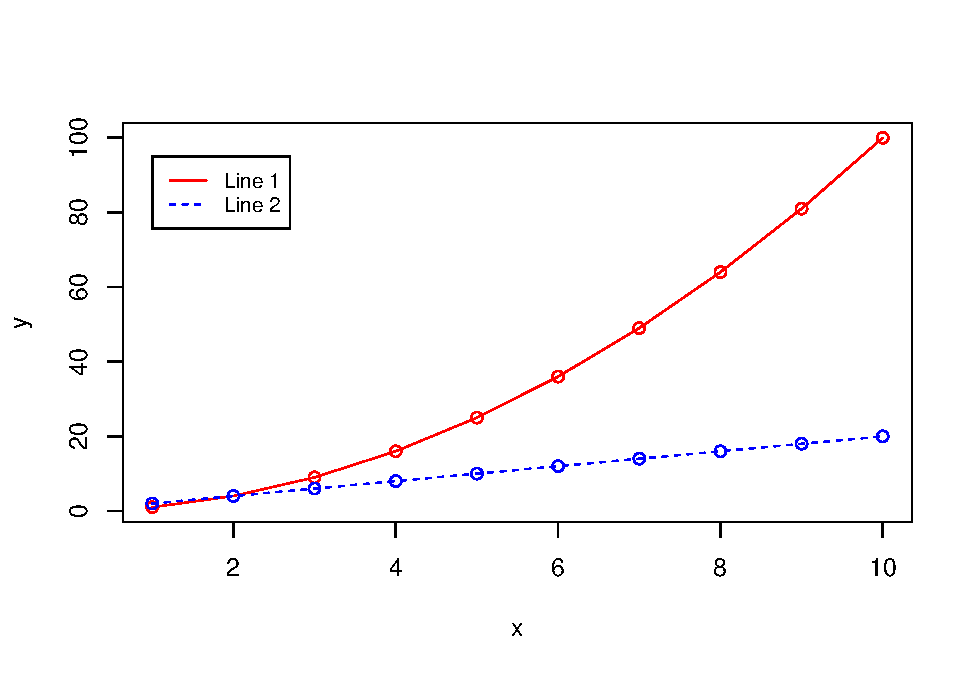
\includegraphics[width=0.7\linewidth]{Metode_Numerik_files/figure-latex/legend-1} 

}

\caption{Menambahkan legend}\label{fig:legend}
\end{figure}

Kita dapat menambahkan judul, merubah font, dan merubah warna backgroud pada legend. Argumen yang ditambahkan pada legend adalah sebagai berikut:

\begin{enumerate}
\def\labelenumi{\alph{enumi}.}
\tightlist
\item
  \textbf{title}: Judul legend
\item
  \textbf{text.font}: integer yang menunjukkan \emph{font style} pada teks legend. Nilai yang dapat dimasukkan adalah sebagai berikut:

  \begin{itemize}
  \tightlist
  \item
    \textbf{1}: normal
  \item
    \textbf{2}: cetak tebal
  \item
    \textbf{3}: cetak miring
  \item
    \textbf{4}: cetak tebal dan miring.
  \end{itemize}
\item
  \textbf{bg}: warna background legend box.
\end{enumerate}

Berikut adalah penerapan sintaks dan output yang dihasilkan pada Gambar \ref{fig:legend2}:

\begin{Shaded}
\begin{Highlighting}[]
\CommentTok{\# membuat line plot}
\FunctionTok{plot}\NormalTok{(x,y, }\AttributeTok{type=}\StringTok{"o"}\NormalTok{, }\AttributeTok{col=}\StringTok{"red"}\NormalTok{, }\AttributeTok{lty=}\DecValTok{1}\NormalTok{)}

\CommentTok{\# menambahkan line plot}
\FunctionTok{lines}\NormalTok{(x,z, }\AttributeTok{type=}\StringTok{"o"}\NormalTok{, }\AttributeTok{col=}\StringTok{"blue"}\NormalTok{, }\AttributeTok{lty=}\DecValTok{2}\NormalTok{)}

\CommentTok{\# menambahkan legend}
\FunctionTok{legend}\NormalTok{(}\DecValTok{1}\NormalTok{, }\DecValTok{95}\NormalTok{, }\AttributeTok{legend=}\FunctionTok{c}\NormalTok{(}\StringTok{"Line 1"}\NormalTok{, }\StringTok{"Line 2"}\NormalTok{),}
       \AttributeTok{col=}\FunctionTok{c}\NormalTok{(}\StringTok{"red"}\NormalTok{, }\StringTok{"blue"}\NormalTok{), }\AttributeTok{lty=}\DecValTok{1}\SpecialCharTok{:}\DecValTok{2}\NormalTok{, }\AttributeTok{cex=}\FloatTok{0.8}\NormalTok{,}
       \AttributeTok{title=}\StringTok{"Line types"}\NormalTok{, }\AttributeTok{text.font=}\DecValTok{4}\NormalTok{, }\AttributeTok{bg=}\StringTok{\textquotesingle{}lightblue\textquotesingle{}}\NormalTok{)}
\end{Highlighting}
\end{Shaded}

\begin{figure}

{\centering 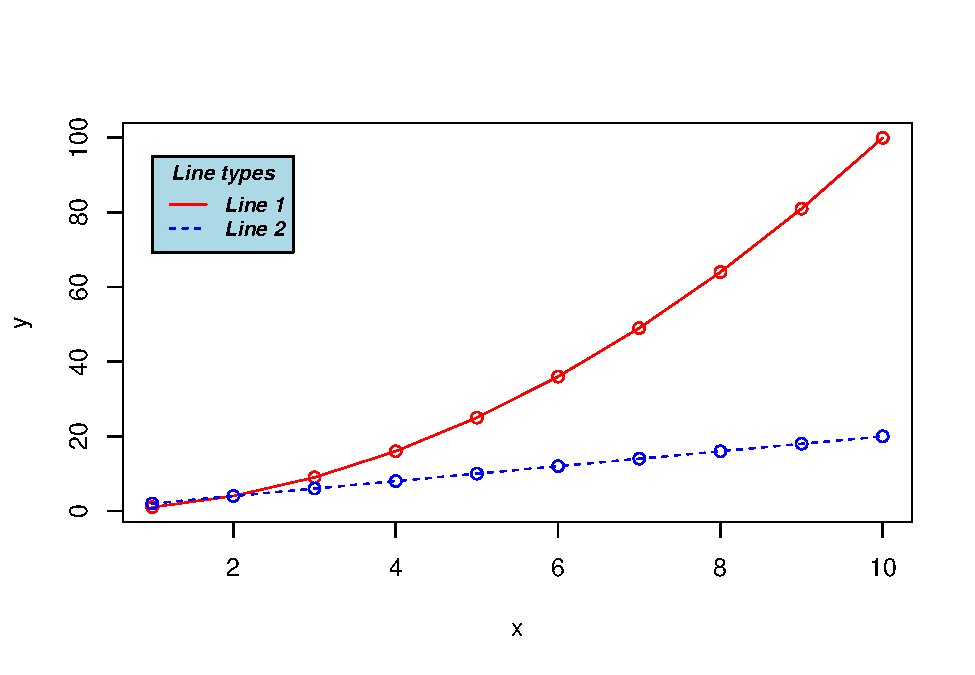
\includegraphics[width=0.7\linewidth]{Metode_Numerik_files/figure-latex/legend2-1} 

}

\caption{Menambahkan legend (2)}\label{fig:legend2}
\end{figure}

Kita dapat melakukan kustomisasi pada border dari legend melalui argumen \texttt{box.lty=}(jenis garis), \texttt{box.lwd=}(ukuran garis), dan \texttt{box.col=}(warna box). Berikut adalah penerapan argumen tersebut beserta output yang dihasilkan pada Gambar \ref{fig:legend3}:

\begin{Shaded}
\begin{Highlighting}[]
\CommentTok{\# membuat line plot}
\FunctionTok{plot}\NormalTok{(x,y, }\AttributeTok{type=}\StringTok{"o"}\NormalTok{, }\AttributeTok{col=}\StringTok{"red"}\NormalTok{, }\AttributeTok{lty=}\DecValTok{1}\NormalTok{)}

\CommentTok{\# menambahkan line plot}
\FunctionTok{lines}\NormalTok{(x,z, }\AttributeTok{type=}\StringTok{"o"}\NormalTok{, }\AttributeTok{col=}\StringTok{"blue"}\NormalTok{, }\AttributeTok{lty=}\DecValTok{2}\NormalTok{)}

\CommentTok{\# menambahkan legend}
\FunctionTok{legend}\NormalTok{(}\DecValTok{1}\NormalTok{, }\DecValTok{95}\NormalTok{, }\AttributeTok{legend=}\FunctionTok{c}\NormalTok{(}\StringTok{"Line 1"}\NormalTok{, }\StringTok{"Line 2"}\NormalTok{),}
       \AttributeTok{col=}\FunctionTok{c}\NormalTok{(}\StringTok{"red"}\NormalTok{, }\StringTok{"blue"}\NormalTok{), }\AttributeTok{lty=}\DecValTok{1}\SpecialCharTok{:}\DecValTok{2}\NormalTok{, }\AttributeTok{cex=}\FloatTok{0.8}\NormalTok{,}
       \AttributeTok{title=}\StringTok{"Line types"}\NormalTok{, }\AttributeTok{text.font=}\DecValTok{4}\NormalTok{, }\AttributeTok{bg=}\StringTok{\textquotesingle{}white\textquotesingle{}}\NormalTok{,}
       \AttributeTok{box.lty=}\DecValTok{2}\NormalTok{, }\AttributeTok{box.lwd=}\DecValTok{2}\NormalTok{, }\AttributeTok{box.col=}\StringTok{"steelblue"}\NormalTok{)}
\end{Highlighting}
\end{Shaded}

\begin{figure}

{\centering 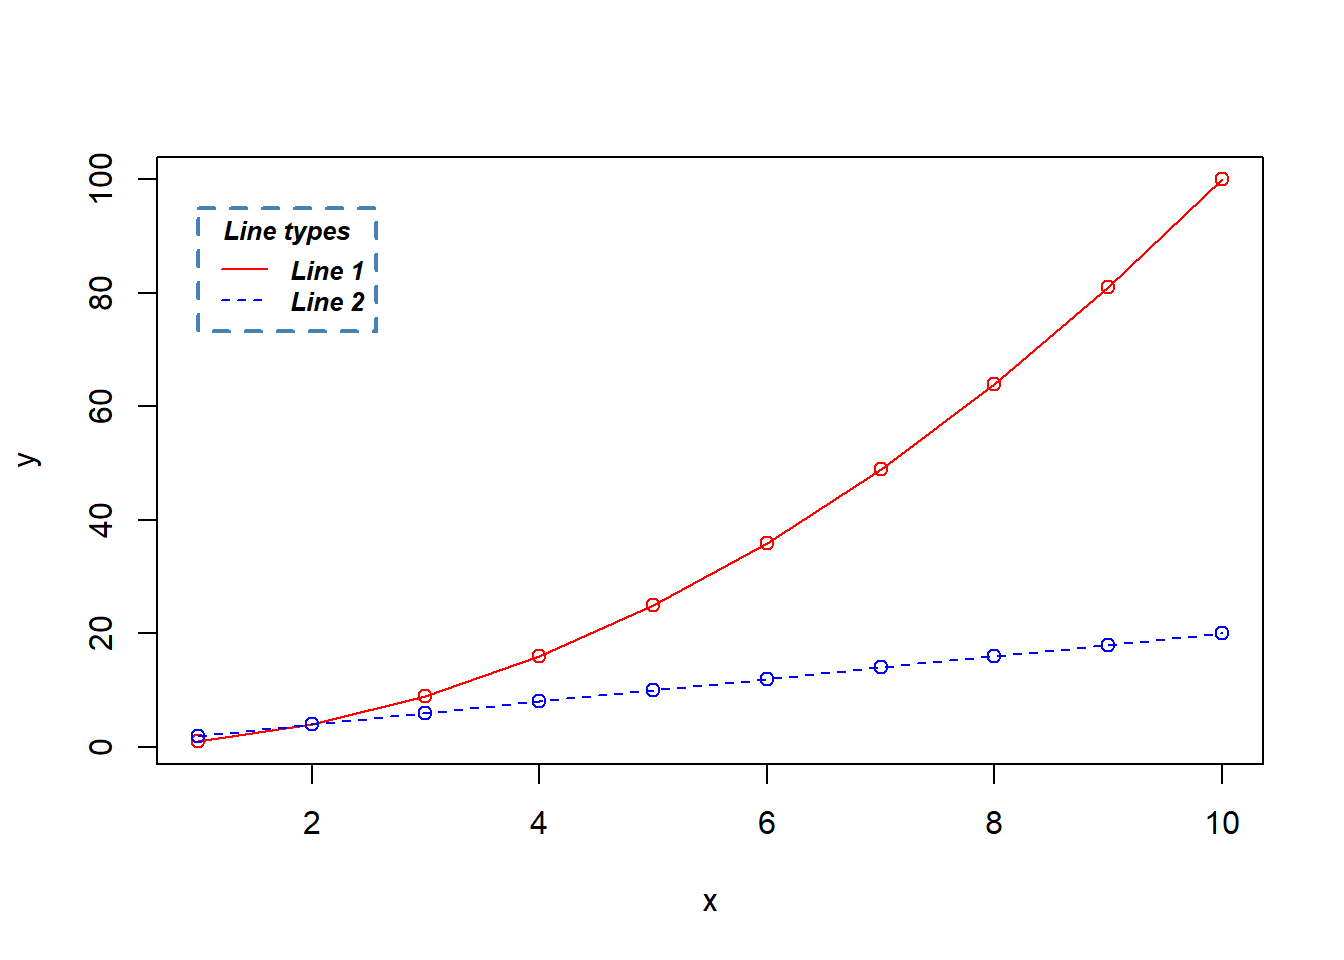
\includegraphics[width=0.7\linewidth]{Metode_Numerik_files/figure-latex/legend3-1} 

}

\caption{Menambahkan legend (3)}\label{fig:legend3}
\end{figure}

Selain menggunakan koordinat, kita juga dapat melakukan kustomisasi posisi legend menggunakan \emph{keyword} seperti: bottomright'', ``bottom'', ``bottomleft'', ``left'', ``topleft'', ``top'', ``topright'', ``right'' and ``center''. Sejumlah kustomisasi legend berdasarkan \emph{keyword} disajikan pada Gambar \ref{fig:legend4}:

\begin{Shaded}
\begin{Highlighting}[]
\CommentTok{\# plot}
\FunctionTok{plot}\NormalTok{(x,y, }\AttributeTok{type =} \StringTok{"n"}\NormalTok{)}

\CommentTok{\# posisi kiri atas, inset =0.05}
\FunctionTok{legend}\NormalTok{(}\StringTok{"topleft"}\NormalTok{,}
  \AttributeTok{legend =} \StringTok{"(x,y)"}\NormalTok{,}
  \AttributeTok{title =} \StringTok{"topleft, inset = .05"}\NormalTok{,}
  \AttributeTok{inset =} \FloatTok{0.05}\NormalTok{)}
\CommentTok{\# posisi atas}
\FunctionTok{legend}\NormalTok{(}\StringTok{"top"}\NormalTok{,}
       \AttributeTok{legend =} \StringTok{"(x,y)"}\NormalTok{,}
       \AttributeTok{title =} \StringTok{"top"}\NormalTok{)}
\CommentTok{\# posisi kanan atas inset = .02}
\FunctionTok{legend}\NormalTok{(}\StringTok{"topright"}\NormalTok{,}
       \AttributeTok{legend =} \StringTok{"(x,y)"}\NormalTok{,}
       \AttributeTok{title =} \StringTok{"topright, inset = .02"}\NormalTok{,}
       \AttributeTok{inset =} \FloatTok{0.02}\NormalTok{)}
\CommentTok{\# posisi kiri}
\FunctionTok{legend}\NormalTok{(}\StringTok{"left"}\NormalTok{,}
       \AttributeTok{legend =} \StringTok{"(x,y)"}\NormalTok{,}
       \AttributeTok{title =} \StringTok{"left"}\NormalTok{)}
\CommentTok{\# posisi tengah}
\FunctionTok{legend}\NormalTok{(}\StringTok{"center"}\NormalTok{,}
       \AttributeTok{legend =} \StringTok{"(x,y)"}\NormalTok{,}
       \AttributeTok{title =} \StringTok{"center"}\NormalTok{)}
\CommentTok{\# posisi kanan}
\FunctionTok{legend}\NormalTok{(}\StringTok{"right"}\NormalTok{,}
       \AttributeTok{legend =} \StringTok{"(x,y)"}\NormalTok{,}
       \AttributeTok{title =} \StringTok{"right"}\NormalTok{)}
\CommentTok{\# posisi kiri bawah}
\FunctionTok{legend}\NormalTok{(}\StringTok{"bottomleft"}\NormalTok{,}
       \AttributeTok{legend =} \StringTok{"(x,y)"}\NormalTok{,}
       \AttributeTok{title =} \StringTok{"bottomleft"}\NormalTok{)}
\CommentTok{\# posisi bawah}
\FunctionTok{legend}\NormalTok{(}\StringTok{"bottom"}\NormalTok{,}
       \AttributeTok{legend =} \StringTok{"(x,y)"}\NormalTok{,}
       \AttributeTok{title =} \StringTok{"bottom"}\NormalTok{)}
\CommentTok{\# posisi kanan bawah}
\FunctionTok{legend}\NormalTok{(}\StringTok{"bottomright"}\NormalTok{,}
       \AttributeTok{legend =} \StringTok{"(x,y)"}\NormalTok{,}
       \AttributeTok{title =} \StringTok{"bottomright"}\NormalTok{)}
\end{Highlighting}
\end{Shaded}

\begin{figure}

{\centering 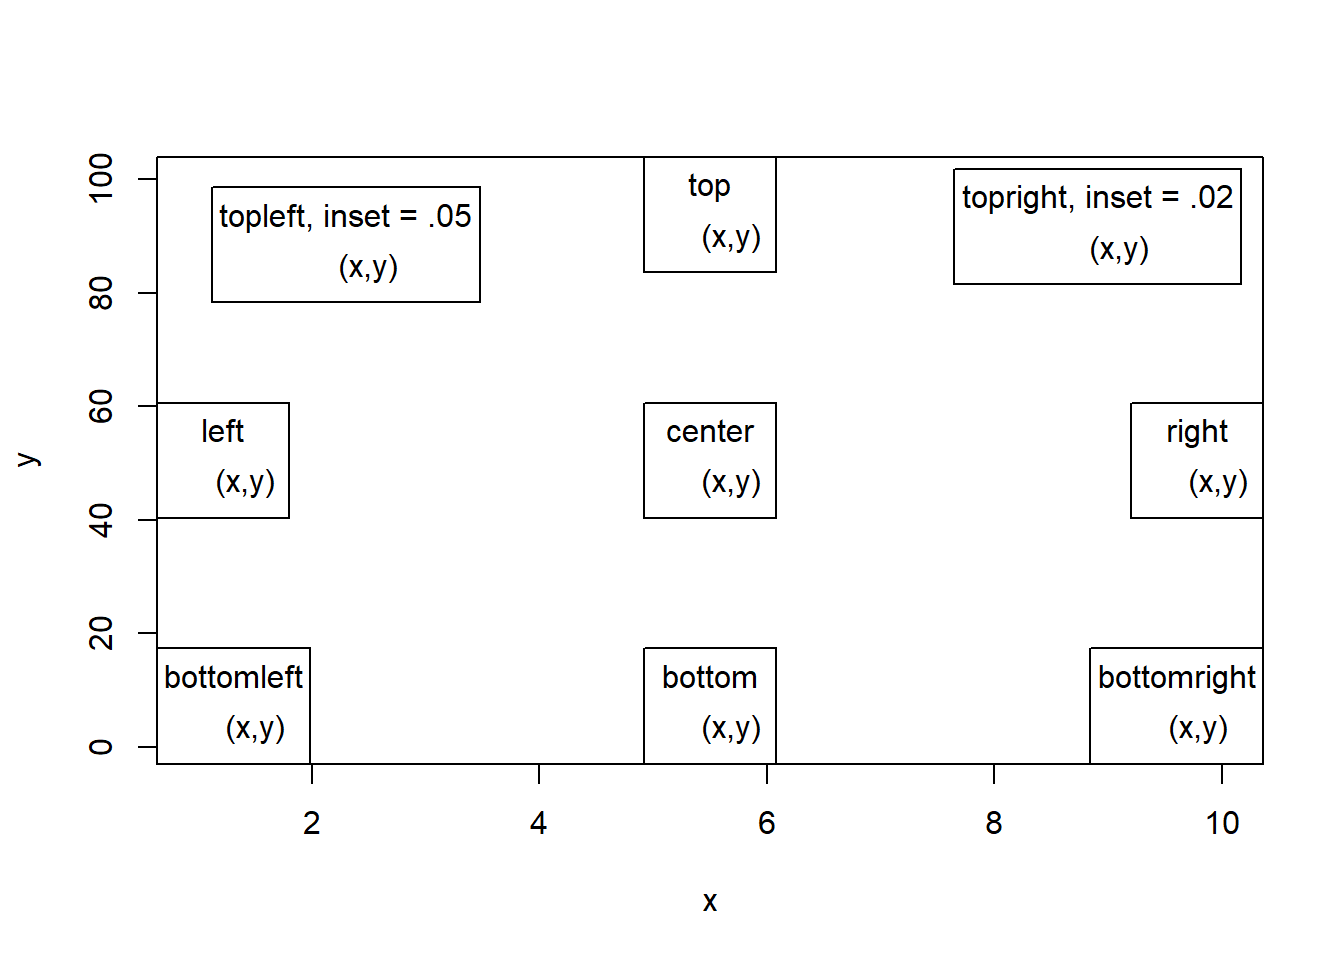
\includegraphics[width=0.7\linewidth]{Metode_Numerik_files/figure-latex/legend4-1} 

}

\caption{Kustomisasi posisi legend}\label{fig:legend4}
\end{figure}

\hypertarget{addtext}{%
\subsection{Menambahkan Teks Pada Grafik}\label{addtext}}

Teks pada grafik dapat kita tambahkan baik sebagai keterangan yang menunjukkan label suatu observasi, keterangan tambahan disekitar bingkai grafik, maupun sebuah persamaan yang ada pada bidang grafik. Untuk menambahkannya kita dapat menggunakan dua buah fungsi yaitu: \texttt{text()} dan \texttt{mtext()}.

FUngsi \texttt{text()} berguna untuk menambahkan teks di dalam bidang grafik seperti label titik observasi dan persamaan di dalam bidang grafik. Format yang digunakan adalah sebagai berikut:

\begin{Shaded}
\begin{Highlighting}[]
\FunctionTok{text}\NormalTok{(x, y, labels)}
\end{Highlighting}
\end{Shaded}

\begin{quote}
\textbf{Catatan:}

\begin{itemize}
\tightlist
\item
  \textbf{x} dan \textbf{y}: vektor numerik yang menunjukkan koordinat posisi teks.
\item
  \textbf{labels}: vektor karakter yang menunjukkan teks yang hendak ditulis.
\end{itemize}
\end{quote}

Berikut adalah contoh sintaks untuk memberi label pada sejumlah data yang memiliki kriteria yang kita inginkan dan output yang dihasilkan pada Gambar \ref{fig:text}:

\begin{Shaded}
\begin{Highlighting}[]
\CommentTok{\# tandai observasi yang memiliki nilai}
\CommentTok{\# mpg \textless{} 15 dan wt \textgreater{} 5}
\NormalTok{d }\OtherTok{\textless{}{-}}\NormalTok{ mtcars[mtcars}\SpecialCharTok{$}\NormalTok{wt }\SpecialCharTok{\textgreater{}=} \DecValTok{5} \SpecialCharTok{\&}\NormalTok{ mtcars}\SpecialCharTok{$}\NormalTok{mpg }\SpecialCharTok{\textless{}=} \DecValTok{15}\NormalTok{, ]}


\CommentTok{\# plot}
\FunctionTok{plot}\NormalTok{(mtcars}\SpecialCharTok{$}\NormalTok{wt, mtcars}\SpecialCharTok{$}\NormalTok{mpg, }\AttributeTok{main=}\StringTok{"Milage vs. Car Weight"}\NormalTok{,}
      \AttributeTok{xlab=}\StringTok{"Weight"}\NormalTok{, }\AttributeTok{ylab=}\StringTok{"Miles/(US) gallon"}\NormalTok{)}

\CommentTok{\# menambahkan text}
\FunctionTok{text}\NormalTok{(d}\SpecialCharTok{$}\NormalTok{wt, d}\SpecialCharTok{$}\NormalTok{mpg,  }\FunctionTok{row.names}\NormalTok{(d),}
     \AttributeTok{cex=}\FloatTok{0.65}\NormalTok{, }\AttributeTok{pos=}\DecValTok{3}\NormalTok{,}\AttributeTok{col=}\StringTok{"red"}\NormalTok{)}
\end{Highlighting}
\end{Shaded}

\begin{figure}

{\centering 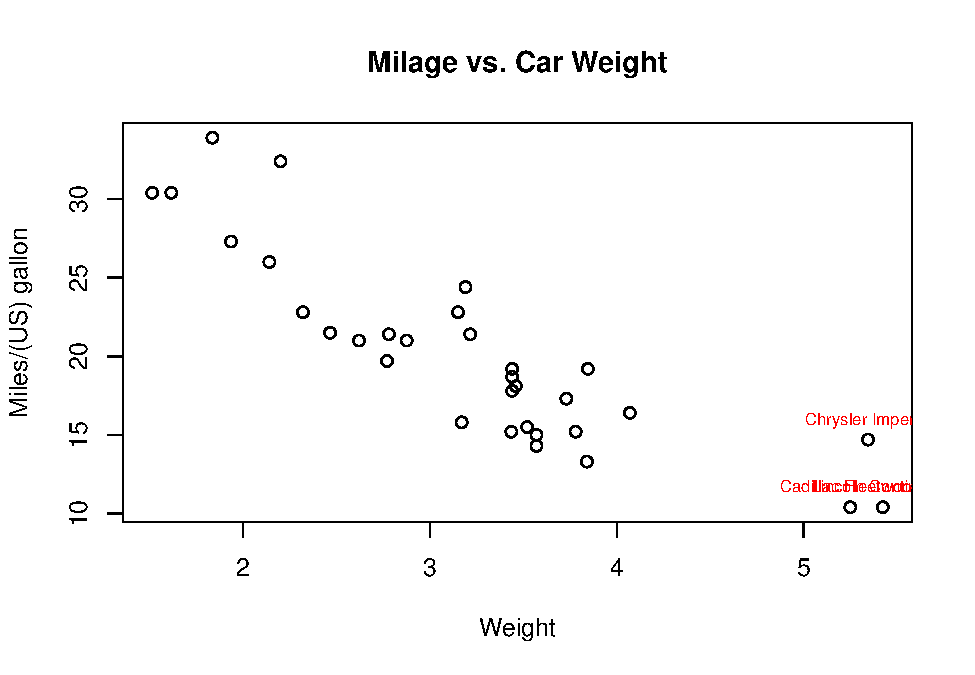
\includegraphics[width=0.7\linewidth]{Metode_Numerik_files/figure-latex/text-1} 

}

\caption{Menambahkan teks}\label{fig:text}
\end{figure}

Sedangkan sintaks berikut adalah contoh bagaimana menambahkan persamaan kedalam bidang grafik dan output yang dihasilkan pada Gambar \ref{fig:text2}:

\begin{Shaded}
\begin{Highlighting}[]
\FunctionTok{plot}\NormalTok{(}\DecValTok{1}\SpecialCharTok{:}\DecValTok{10}\NormalTok{, }\DecValTok{1}\SpecialCharTok{:}\DecValTok{10}\NormalTok{, }
     \AttributeTok{main=}\StringTok{"text(...) examples}\SpecialCharTok{\textbackslash{}n}\StringTok{\textasciitilde{}\textasciitilde{}\textasciitilde{}\textasciitilde{}\textasciitilde{}\textasciitilde{}\textasciitilde{}\textasciitilde{}\textasciitilde{}\textasciitilde{}\textasciitilde{}"}\NormalTok{)}
\FunctionTok{text}\NormalTok{(}\DecValTok{4}\NormalTok{, }\DecValTok{9}\NormalTok{, }\FunctionTok{expression}\NormalTok{(}\FunctionTok{hat}\NormalTok{(beta) }\SpecialCharTok{==}\NormalTok{ (X}\SpecialCharTok{\^{}}\NormalTok{t }\SpecialCharTok{*}\NormalTok{ X)}\SpecialCharTok{\^{}}\NormalTok{\{}\SpecialCharTok{{-}}\DecValTok{1}\NormalTok{\} }\SpecialCharTok{*}\NormalTok{ X}\SpecialCharTok{\^{}}\NormalTok{t }\SpecialCharTok{*}\NormalTok{ y))}
\FunctionTok{text}\NormalTok{(}\DecValTok{7}\NormalTok{, }\DecValTok{4}\NormalTok{, }\FunctionTok{expression}\NormalTok{(}\FunctionTok{bar}\NormalTok{(x) }\SpecialCharTok{==} \FunctionTok{sum}\NormalTok{(}\FunctionTok{frac}\NormalTok{(x[i], n), i}\SpecialCharTok{==}\DecValTok{1}\NormalTok{, n)))}
\end{Highlighting}
\end{Shaded}

\begin{figure}

{\centering 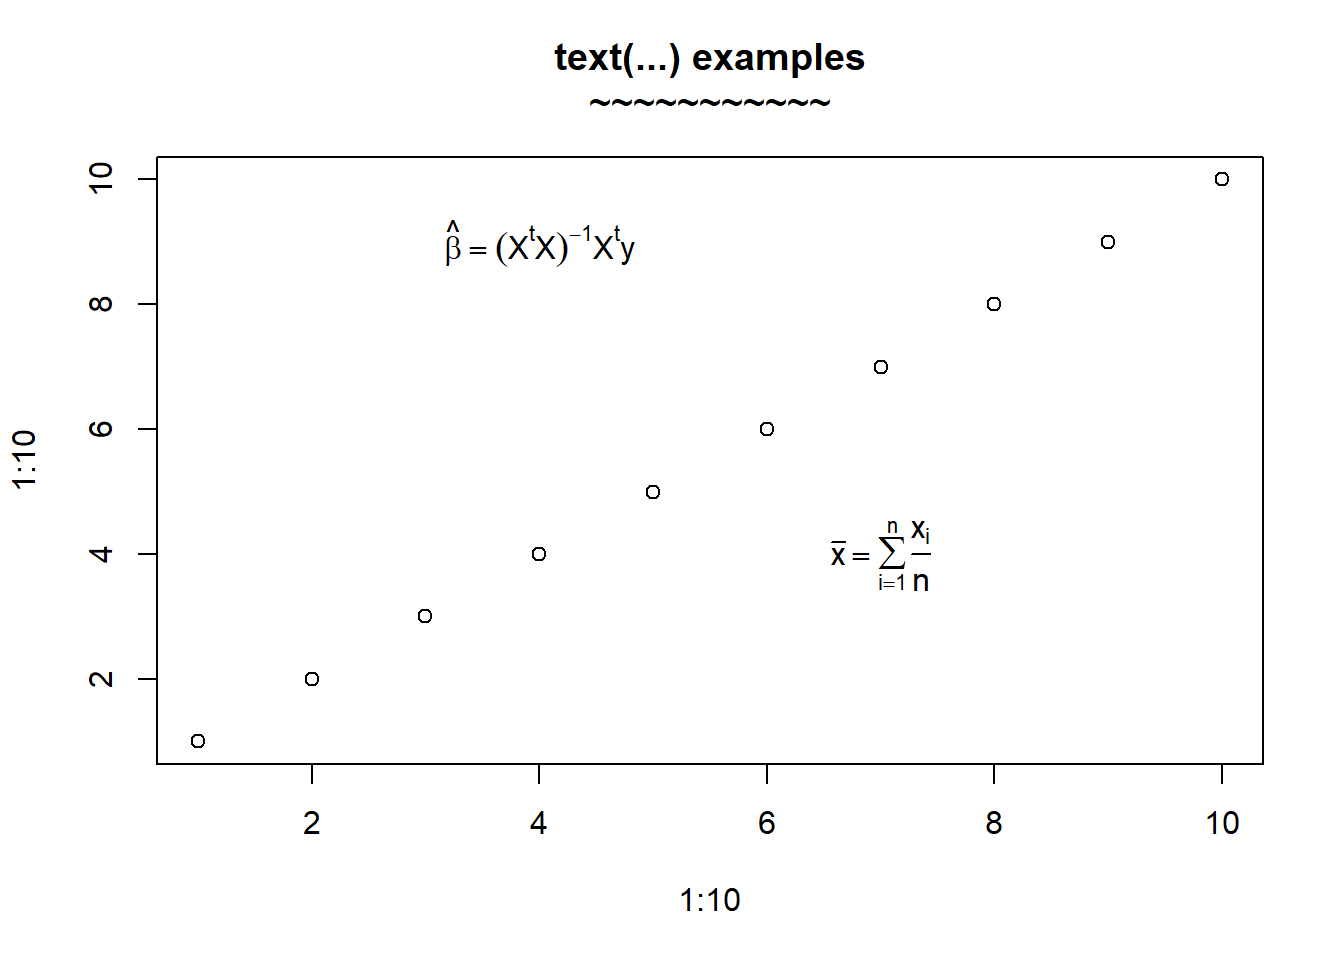
\includegraphics[width=0.7\linewidth]{Metode_Numerik_files/figure-latex/text2-1} 

}

\caption{Menambahkan teks (2)}\label{fig:text2}
\end{figure}

Fungsi \texttt{mtext()} berguna untuk menambahkan teks pada frame sekitar bidang grafik. Format yang digunakan adalah sebagai berikut:

\begin{Shaded}
\begin{Highlighting}[]
\FunctionTok{mtext}\NormalTok{(text, }\AttributeTok{side=}\DecValTok{3}\NormalTok{)}
\end{Highlighting}
\end{Shaded}

\begin{quote}
\textbf{Catatan:}

\begin{itemize}
\tightlist
\item
  \textbf{text}: teks yang akan ditulis.
\item
  \textbf{side}: integer yang menunjukkan lokasi teks yang akan ditulis. Nilai yang dapat dimasukkan antara lain:
\item
  1: bawah
\item
  2: kiri
\item
  3: atas
\item
  4: kanan.
\end{itemize}
\end{quote}

Berikut adalah contoh penerapan dan output yang dihasilkan pada Gambar \ref{fig:text3}:

\begin{Shaded}
\begin{Highlighting}[]
\FunctionTok{plot}\NormalTok{(}\DecValTok{1}\SpecialCharTok{:}\DecValTok{10}\NormalTok{, }\DecValTok{1}\SpecialCharTok{:}\DecValTok{10}\NormalTok{, }
     \AttributeTok{main=}\StringTok{"mtext(...) examples}\SpecialCharTok{\textbackslash{}n}\StringTok{\textasciitilde{}\textasciitilde{}\textasciitilde{}\textasciitilde{}\textasciitilde{}\textasciitilde{}\textasciitilde{}\textasciitilde{}\textasciitilde{}\textasciitilde{}\textasciitilde{}"}\NormalTok{)}
\FunctionTok{mtext}\NormalTok{(}\StringTok{"Magic function"}\NormalTok{, }\AttributeTok{side=}\DecValTok{3}\NormalTok{)}
\end{Highlighting}
\end{Shaded}

\begin{figure}

{\centering 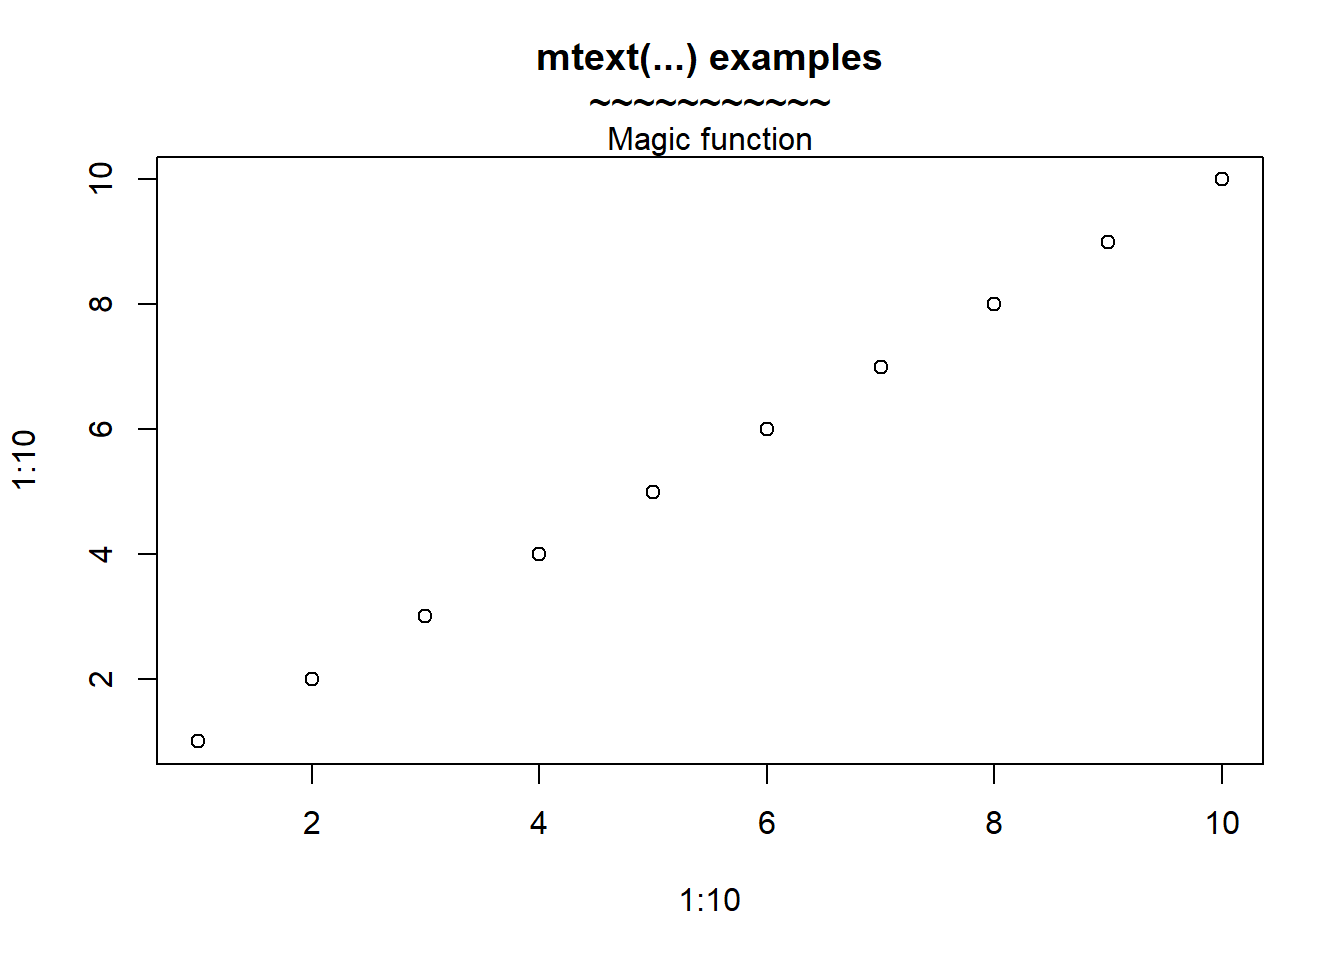
\includegraphics[width=0.7\linewidth]{Metode_Numerik_files/figure-latex/text3-1} 

}

\caption{Menambahkan teks (3)}\label{fig:text3}
\end{figure}

\hypertarget{addlines}{%
\subsection{Menambahkan Garis Pada Plot}\label{addlines}}

Fungsi \texttt{abline()} dapat digunakan untuk menamabahkan garis pada plot. Garis yang ditambahkan dapat berupa garis vertikal, horizontal, maupun garis regresi. Format yang digunakan adalah sebagi berikut:

\begin{Shaded}
\begin{Highlighting}[]
\FunctionTok{abline}\NormalTok{(}\AttributeTok{v=}\NormalTok{y)}
\end{Highlighting}
\end{Shaded}

Berikut adalah contoh sintaks bagaimana menambahkan garis pada sebuah plot dan output yang dihasilkan disajikan pada Gambar \ref{fig:abline}:

\begin{Shaded}
\begin{Highlighting}[]
\CommentTok{\# membuat plot}
\FunctionTok{plot}\NormalTok{(mtcars}\SpecialCharTok{$}\NormalTok{wt, mtcars}\SpecialCharTok{$}\NormalTok{mpg, }\AttributeTok{main=}\StringTok{"Milage vs. Car Weight"}\NormalTok{,}
      \AttributeTok{xlab=}\StringTok{"Weight"}\NormalTok{, }\AttributeTok{ylab=}\StringTok{"Miles/(US) gallon"}\NormalTok{)}

\CommentTok{\# menambahkan garis vertikal di titik rata{-}rata weight}
\FunctionTok{abline}\NormalTok{(}\AttributeTok{v=}\FunctionTok{mean}\NormalTok{(mtcars}\SpecialCharTok{$}\NormalTok{wt), }\AttributeTok{col=}\StringTok{"red"}\NormalTok{, }\AttributeTok{lwd=}\DecValTok{3}\NormalTok{, }\AttributeTok{lty=}\DecValTok{2}\NormalTok{)}

\CommentTok{\# menambahkan garis horizontal di titik rata{-}rata  mpg}
\FunctionTok{abline}\NormalTok{(}\AttributeTok{h=}\FunctionTok{mean}\NormalTok{(mtcars}\SpecialCharTok{$}\NormalTok{mpg), }\AttributeTok{col=}\StringTok{"blue"}\NormalTok{, }\AttributeTok{lwd=}\DecValTok{3}\NormalTok{, }\AttributeTok{lty=}\DecValTok{3}\NormalTok{)}

\CommentTok{\# menambahkan garis regresi}
\FunctionTok{abline}\NormalTok{(}\FunctionTok{lm}\NormalTok{(mpg}\SpecialCharTok{\textasciitilde{}}\NormalTok{wt, }\AttributeTok{data=}\NormalTok{mtcars), }\AttributeTok{lwd=}\DecValTok{4}\NormalTok{, }\AttributeTok{lty=}\DecValTok{4}\NormalTok{)}
\end{Highlighting}
\end{Shaded}

\begin{figure}

{\centering 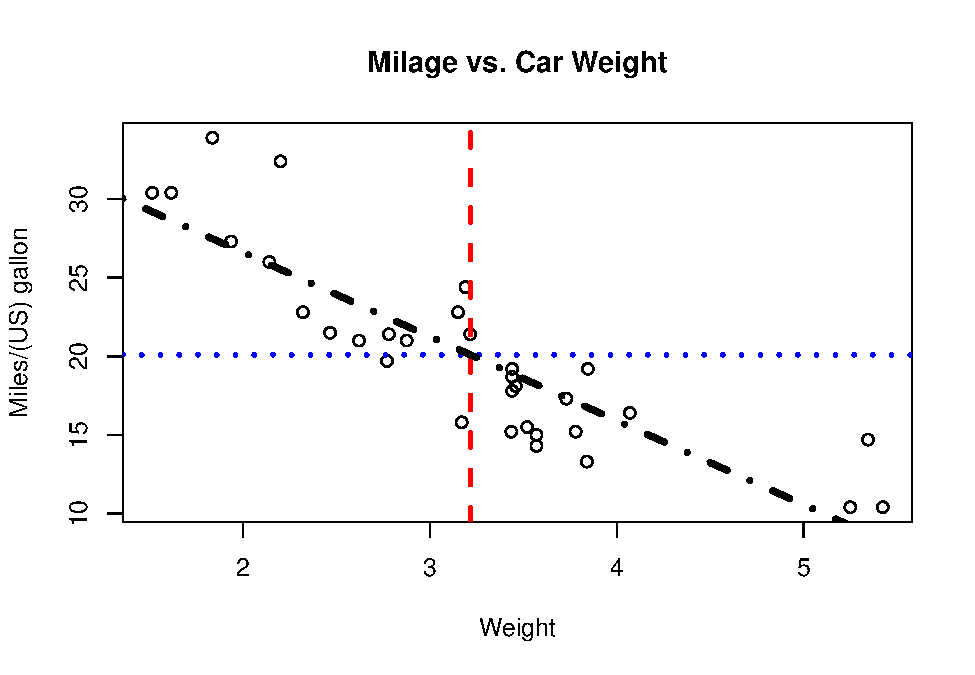
\includegraphics[width=0.7\linewidth]{Metode_Numerik_files/figure-latex/abline-1} 

}

\caption{Menambahkan garis}\label{fig:abline}
\end{figure}

\hypertarget{changepoint}{%
\subsection{Merubah Simbol plot dan Jenis Garis}\label{changepoint}}

Simbol plot (jenis titik) dapat diubah dengan menambahkan argumen \texttt{pch=} pada plot. Nilai yang dimasukkan pada argumen tersebut adalah integer dengan kemungkinan nilai sebagai berikut:

\begin{itemize}
\tightlist
\item
  pch = 0,square
\item
  pch = 1,circle (default)
\item
  pch = 2,triangle point up
\item
  pch = 3,plus
\item
  pch = 4,cross
\item
  pch = 5,diamond
\item
  pch = 6,triangle point down
\item
  pch = 7,square cross
\item
  pch = 8,star
\item
  pch = 9,diamond plus
\item
  pch = 10,circle plus
\item
  pch = 11,triangles up and down
\item
  pch = 12,square plus
\item
  pch = 13,circle cross
\item
  pch = 14,square and triangle down
\item
  pch = 15, filled square
\item
  pch = 16, filled circle
\item
  pch = 17, filled triangle point-up
\item
  pch = 18, filled diamond
\item
  pch = 19, solid circle
\item
  pch = 20,bullet (smaller circle)
\item
  pch = 21, filled circle blue
\item
  pch = 22, filled square blue
\item
  pch = 23, filled diamond blue
\item
  pch = 24, filled triangle point-up blue
\item
  pch = 25, filled triangle point down blue
\end{itemize}

Untuk lebih memahami bentuk simbol tersebut, penulis akan menyajikan sintaks yang menampilkan seluruh simbol tersebut pada satu grafik. Output yang dihasilkan disajikan pada Gambar \ref{fig:symbol}:

\begin{Shaded}
\begin{Highlighting}[]
\NormalTok{generateRPointShapes}\OtherTok{\textless{}{-}}\ControlFlowTok{function}\NormalTok{()\{}
  \CommentTok{\# menentukan parameter plot}
\NormalTok{  oldPar}\OtherTok{\textless{}{-}}\FunctionTok{par}\NormalTok{()}
  \FunctionTok{par}\NormalTok{(}\AttributeTok{font=}\DecValTok{2}\NormalTok{, }\AttributeTok{mar=}\FunctionTok{c}\NormalTok{(}\FloatTok{0.5}\NormalTok{,}\DecValTok{0}\NormalTok{,}\DecValTok{0}\NormalTok{,}\DecValTok{0}\NormalTok{))}
  \CommentTok{\# produksi titik axis}
\NormalTok{  y}\OtherTok{=}\FunctionTok{rev}\NormalTok{(}\FunctionTok{c}\NormalTok{(}\FunctionTok{rep}\NormalTok{(}\DecValTok{1}\NormalTok{,}\DecValTok{6}\NormalTok{),}\FunctionTok{rep}\NormalTok{(}\DecValTok{2}\NormalTok{,}\DecValTok{5}\NormalTok{), }\FunctionTok{rep}\NormalTok{(}\DecValTok{3}\NormalTok{,}\DecValTok{5}\NormalTok{), }\FunctionTok{rep}\NormalTok{(}\DecValTok{4}\NormalTok{,}\DecValTok{5}\NormalTok{), }\FunctionTok{rep}\NormalTok{(}\DecValTok{5}\NormalTok{,}\DecValTok{5}\NormalTok{)))}
\NormalTok{  x}\OtherTok{=}\FunctionTok{c}\NormalTok{(}\FunctionTok{rep}\NormalTok{(}\DecValTok{1}\SpecialCharTok{:}\DecValTok{5}\NormalTok{,}\DecValTok{5}\NormalTok{),}\DecValTok{6}\NormalTok{)}
  \CommentTok{\# plot seluruh titik dan label}
  \FunctionTok{plot}\NormalTok{(x, y, }\AttributeTok{pch =} \DecValTok{0}\SpecialCharTok{:}\DecValTok{25}\NormalTok{, }\AttributeTok{cex=}\FloatTok{1.5}\NormalTok{, }\AttributeTok{ylim=}\FunctionTok{c}\NormalTok{(}\DecValTok{1}\NormalTok{,}\FloatTok{5.5}\NormalTok{), }\AttributeTok{xlim=}\FunctionTok{c}\NormalTok{(}\DecValTok{1}\NormalTok{,}\FloatTok{6.5}\NormalTok{), }
       \AttributeTok{axes=}\ConstantTok{FALSE}\NormalTok{, }\AttributeTok{xlab=}\StringTok{""}\NormalTok{, }\AttributeTok{ylab=}\StringTok{""}\NormalTok{, }\AttributeTok{bg=}\StringTok{"blue"}\NormalTok{)}
  \FunctionTok{text}\NormalTok{(x, y, }\AttributeTok{labels=}\DecValTok{0}\SpecialCharTok{:}\DecValTok{25}\NormalTok{, }\AttributeTok{pos=}\DecValTok{3}\NormalTok{)}
  \FunctionTok{par}\NormalTok{(}\AttributeTok{mar=}\NormalTok{oldPar}\SpecialCharTok{$}\NormalTok{mar,}\AttributeTok{font=}\NormalTok{oldPar}\SpecialCharTok{$}\NormalTok{font )}
\NormalTok{\}}

\CommentTok{\# Print}
\FunctionTok{generateRPointShapes}\NormalTok{()}
\end{Highlighting}
\end{Shaded}

\begin{figure}

{\centering 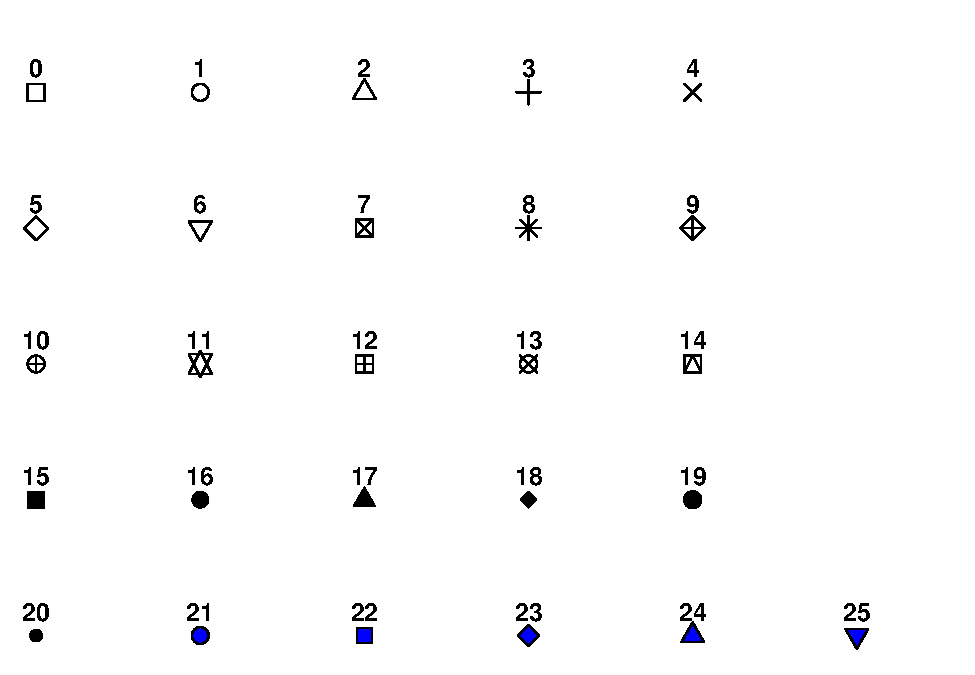
\includegraphics[width=0.7\linewidth]{Metode_Numerik_files/figure-latex/symbol-1} 

}

\caption{Symbol plot}\label{fig:symbol}
\end{figure}

Pada \texttt{R} kita juga dapat mengatur jenis garis yang akan ditampilkan pada plot dengan menambahkan argumen \texttt{lty=} (\emph{line type}) pada fungsi plot. Nilai yang dapat dimasukkan adalah nilai integer. Keterangan masing-masing nilai tersebut adalah sebagai berikut:

\begin{itemize}
\tightlist
\item
  lty = 0, blank
\item
  lty = 1, solid (default)
\item
  lty = 2, dashed
\item
  lty = 3, dotted
\item
  lty = 4, dotdash
\item
  lty = 5, longdash
\item
  lty = 6, twodash
\end{itemize}

Untuk lebih memahaminya, pada sintaks berikut disajikan plot seluruh jenis garis tersebut beserta output yang dihasilkannya pada Gambar \ref{fig:lty}:

\begin{Shaded}
\begin{Highlighting}[]
\NormalTok{generateRLineTypes}\OtherTok{\textless{}{-}}\ControlFlowTok{function}\NormalTok{()\{}
\NormalTok{  oldPar}\OtherTok{\textless{}{-}}\FunctionTok{par}\NormalTok{()}
  \FunctionTok{par}\NormalTok{(}\AttributeTok{font=}\DecValTok{2}\NormalTok{, }\AttributeTok{mar=}\FunctionTok{c}\NormalTok{(}\DecValTok{0}\NormalTok{,}\DecValTok{0}\NormalTok{,}\DecValTok{0}\NormalTok{,}\DecValTok{0}\NormalTok{))}
  \FunctionTok{plot}\NormalTok{(}\DecValTok{1}\NormalTok{, }\AttributeTok{pch=}\StringTok{""}\NormalTok{, }\AttributeTok{ylim=}\FunctionTok{c}\NormalTok{(}\DecValTok{0}\NormalTok{,}\DecValTok{6}\NormalTok{), }\AttributeTok{xlim=}\FunctionTok{c}\NormalTok{(}\DecValTok{0}\NormalTok{,}\FloatTok{0.7}\NormalTok{), }\AttributeTok{axes =} \ConstantTok{FALSE}\NormalTok{ ,}\AttributeTok{xlab=}\StringTok{""}\NormalTok{, }\AttributeTok{ylab=}\StringTok{""}\NormalTok{)}
  \ControlFlowTok{for}\NormalTok{(i }\ControlFlowTok{in} \DecValTok{0}\SpecialCharTok{:}\DecValTok{6}\NormalTok{) }\FunctionTok{lines}\NormalTok{(}\FunctionTok{c}\NormalTok{(}\FloatTok{0.3}\NormalTok{,}\FloatTok{0.7}\NormalTok{), }\FunctionTok{c}\NormalTok{(i,i), }\AttributeTok{lty=}\NormalTok{i, }\AttributeTok{lwd=}\DecValTok{3}\NormalTok{)}
  \FunctionTok{text}\NormalTok{(}\FunctionTok{rep}\NormalTok{(}\FloatTok{0.1}\NormalTok{,}\DecValTok{6}\NormalTok{), }\DecValTok{0}\SpecialCharTok{:}\DecValTok{6}\NormalTok{, }
       \AttributeTok{labels=}\FunctionTok{c}\NormalTok{(}\StringTok{"0.\textquotesingle{}blank\textquotesingle{}"}\NormalTok{, }\StringTok{"1.\textquotesingle{}solid\textquotesingle{}"}\NormalTok{, }\StringTok{"2.\textquotesingle{}dashed\textquotesingle{}"}\NormalTok{, }\StringTok{"3.\textquotesingle{}dotted\textquotesingle{}"}\NormalTok{, }
                \StringTok{"4.\textquotesingle{}dotdash\textquotesingle{}"}\NormalTok{, }\StringTok{"5.\textquotesingle{}longdash\textquotesingle{}"}\NormalTok{, }\StringTok{"6.\textquotesingle{}twodash\textquotesingle{}"}\NormalTok{))}
  \FunctionTok{par}\NormalTok{(}\AttributeTok{mar=}\NormalTok{oldPar}\SpecialCharTok{$}\NormalTok{mar,}\AttributeTok{font=}\NormalTok{oldPar}\SpecialCharTok{$}\NormalTok{font )}
\NormalTok{\}}
\FunctionTok{generateRLineTypes}\NormalTok{()}
\end{Highlighting}
\end{Shaded}

\begin{figure}

{\centering 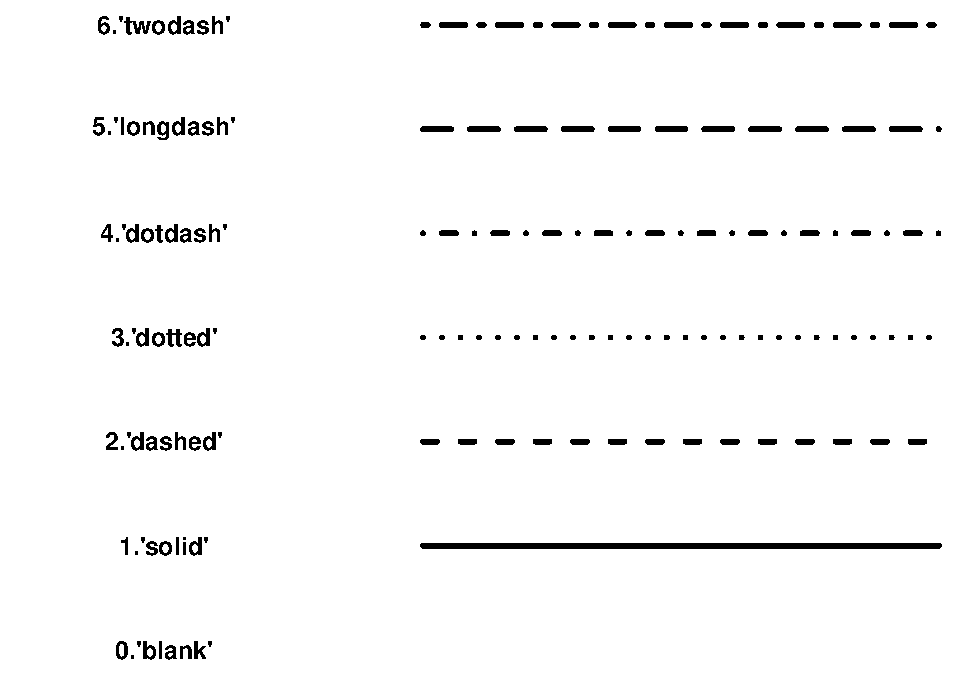
\includegraphics[width=0.7\linewidth]{Metode_Numerik_files/figure-latex/lty-1} 

}

\caption{Line type}\label{fig:lty}
\end{figure}

\hypertarget{mengatur-axis-plot}{%
\subsection{Mengatur Axis Plot}\label{mengatur-axis-plot}}

Kita dapat melakukan pengaturan lebih jauh terhadap axis, seperti: menambahkan axis tambahan pada atas dan bawah frame, mengubah rentang nilai axis, serta kustomisasi \emph{tick mark} pada nilai axis. Hal ini diperlukan karena fungsi grafik dasar \texttt{R} tidak dapat mengatur axis secara otomatis saat plot baru ditambahkan pada plot pertama dan rentang nilai plot baru lebih besar dibanding plot pertama, sehingga sebagian nilai plot baru tidak ditampilkan pada hasil akhir.

Untuk menambahkan axis pada \texttt{R} kita dapat menambahkan fungsi \texttt{axis()} setelah plot dilakukan. Format yang digunakan adalah sebagai berikut:

\begin{Shaded}
\begin{Highlighting}[]
\FunctionTok{axis}\NormalTok{(side, }\AttributeTok{at=}\ConstantTok{NULL}\NormalTok{, }\AttributeTok{labels=}\ConstantTok{TRUE}\NormalTok{)}
\end{Highlighting}
\end{Shaded}

\begin{quote}
\textbf{Catatan:}

\begin{itemize}
\tightlist
\item
  \textbf{side}: nilai integer yang mengidikasikan posisi axix yang hendak ditambahkan. Nilai yang dapat dimasukkan adalah sebagai berikut:

  \begin{itemize}
  \tightlist
  \item
    1: bawah
  \item
    2: kiri
  \item
    3: atas
  \item
    4: kanan.
  \end{itemize}
\item
  \textbf{at}: titik dimana \emph{tick-mark} hendak digambarkan. Nilai yang dapat dimasukkan sama dengan \texttt{side}.
\item
  \textbf{labels}: Teks label \emph{tick-mark}. Dapat juga secara logis menentukan apakah anotasi harus dibuat pada \emph{tick mark}.
\end{itemize}
\end{quote}

Berikut contoh sintaks penerapan fungsi tersebut dan output yang dihasilkan pada Gambar \ref{fig:axis}:

\begin{Shaded}
\begin{Highlighting}[]
\CommentTok{\# membuat vektor numerik}
\NormalTok{x }\OtherTok{\textless{}{-}} \FunctionTok{c}\NormalTok{(}\DecValTok{1}\SpecialCharTok{:}\DecValTok{4}\NormalTok{)}
\NormalTok{y }\OtherTok{\textless{}{-}}\NormalTok{ x}\SpecialCharTok{\^{}}\DecValTok{2}

\CommentTok{\# plot}
\FunctionTok{plot}\NormalTok{(x, y, }\AttributeTok{pch=}\DecValTok{18}\NormalTok{, }\AttributeTok{col=}\StringTok{"red"}\NormalTok{, }\AttributeTok{type=}\StringTok{"b"}\NormalTok{,}
     \AttributeTok{frame=}\ConstantTok{FALSE}\NormalTok{, }\AttributeTok{xaxt=}\StringTok{"n"}\NormalTok{) }\CommentTok{\# Remove x axis}

\CommentTok{\# menambahkan axis}
\CommentTok{\# bawah}
\FunctionTok{axis}\NormalTok{(}\DecValTok{1}\NormalTok{, }\DecValTok{1}\SpecialCharTok{:}\DecValTok{4}\NormalTok{, LETTERS[}\DecValTok{1}\SpecialCharTok{:}\DecValTok{4}\NormalTok{], }\AttributeTok{col.axis=}\StringTok{"blue"}\NormalTok{)}
\CommentTok{\# atas}
\FunctionTok{axis}\NormalTok{(}\DecValTok{3}\NormalTok{, }\AttributeTok{col =} \StringTok{"darkgreen"}\NormalTok{, }\AttributeTok{lty =} \DecValTok{2}\NormalTok{, }\AttributeTok{lwd =} \FloatTok{0.5}\NormalTok{)}
\CommentTok{\# kanan}
\FunctionTok{axis}\NormalTok{(}\DecValTok{4}\NormalTok{, }\AttributeTok{col =} \StringTok{"violet"}\NormalTok{, }\AttributeTok{col.axis =} \StringTok{"dark violet"}\NormalTok{, }\AttributeTok{lwd =} \DecValTok{2}\NormalTok{)}
\end{Highlighting}
\end{Shaded}

\begin{figure}

{\centering 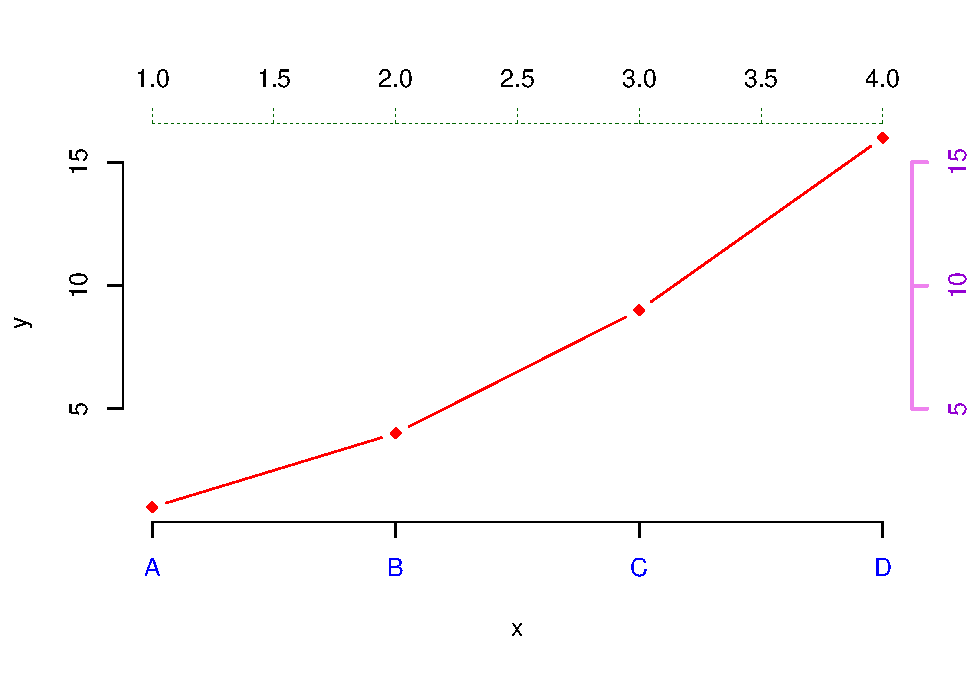
\includegraphics[width=0.7\linewidth]{Metode_Numerik_files/figure-latex/axis-1} 

}

\caption{Modifikasi axis}\label{fig:axis}
\end{figure}

Kita dapat mengubah rentang nilai pada axis menggunakan fungsi \texttt{xlim()} dan \texttt{ylim()} yang menyatakan vektor nilai masimum dan minimum rentang. Selain itu kita dapat juga melakukan tranformasi baik pada sumbu x dan sumbu y. Berikut adalah argumen yang dapat ditambahkan pada fungsi grafik:

\begin{itemize}
\tightlist
\item
  \textbf{xlim}: limit nilai sumbu x dengan format: \texttt{xlim(min,\ max)}.
\item
  \textbf{ylim}: limit nilai sumbu x dengan format: \texttt{ylim(min,\ max)}.
\end{itemize}

Untuk transformasi skala log, kita dapat menambahkan argumen berikut:

\begin{itemize}
\tightlist
\item
  \textbf{log=``x''}: transformasi log sumbu x.
\item
  \textbf{log=``y''}: transformasi log sumbu y.
\item
  \textbf{log=``xy''}: transformasi log sumbu x dan y.
\end{itemize}

Berikut adalah contoh sintaks penerapan argumen tersebut beserta output yang dihasilkan pada Gambar \ref{fig:axis2}:

\begin{Shaded}
\begin{Highlighting}[]
\CommentTok{\# membagi jendela grafik menjadi 1 baris dan 3 kolom}
\FunctionTok{par}\NormalTok{(}\AttributeTok{mfrow=}\FunctionTok{c}\NormalTok{(}\DecValTok{1}\NormalTok{,}\DecValTok{3}\NormalTok{))}

\CommentTok{\# membuat vektor numerik}
\NormalTok{x}\OtherTok{\textless{}{-}}\FunctionTok{c}\NormalTok{(}\DecValTok{1}\SpecialCharTok{:}\DecValTok{10}\NormalTok{); y}\OtherTok{\textless{}{-}}\NormalTok{x}\SpecialCharTok{*}\NormalTok{x}

\CommentTok{\# simple plot}
\FunctionTok{plot}\NormalTok{(x, y)}

\CommentTok{\# plot dengan pengaturan rentang skala}
\FunctionTok{plot}\NormalTok{(x, y, }\AttributeTok{xlim=}\FunctionTok{c}\NormalTok{(}\DecValTok{1}\NormalTok{,}\DecValTok{15}\NormalTok{), }\AttributeTok{ylim=}\FunctionTok{c}\NormalTok{(}\DecValTok{1}\NormalTok{,}\DecValTok{150}\NormalTok{))}

\CommentTok{\# plot dengan transformasi skala log}
\FunctionTok{plot}\NormalTok{(x, y, }\AttributeTok{log=}\StringTok{"y"}\NormalTok{)}
\end{Highlighting}
\end{Shaded}

\begin{figure}

{\centering 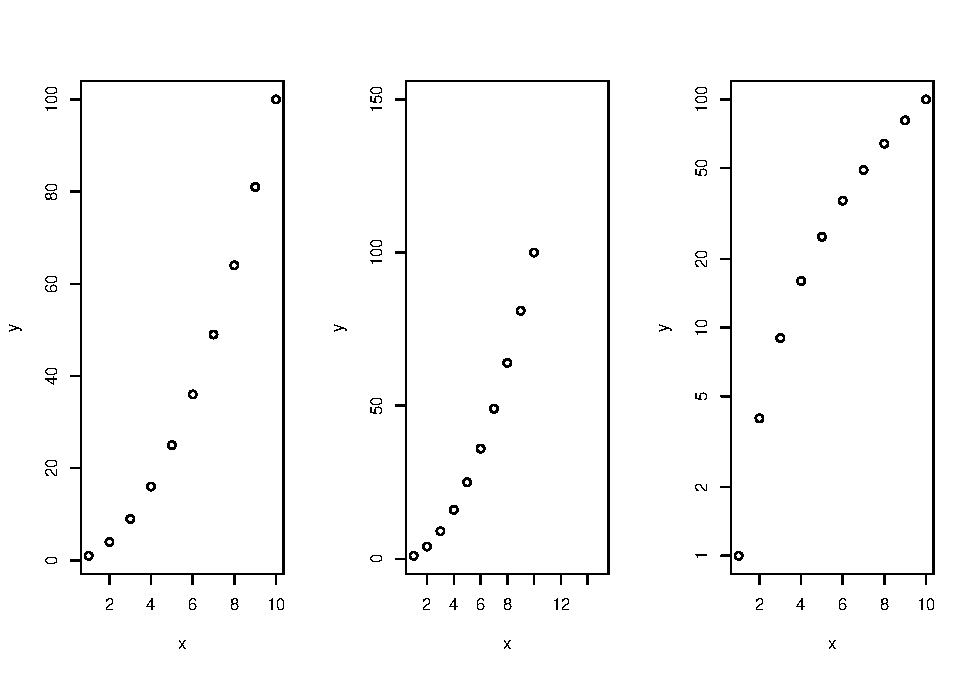
\includegraphics[width=0.8\linewidth]{Metode_Numerik_files/figure-latex/axis2-1} 

}

\caption{Mengubah rentang dan skala axis}\label{fig:axis2}
\end{figure}

Kita dapat melakukan kustomisasi pada \emph{tick mark}. Kustomisasi yang dapat dilakukan adalah merubah warna, \emph{font style}, ukuran font, orientasi, serta menyembunyikan \emph{tick mark}.

Argumen yang ditambahkan adalah sebagai berikut:

\begin{itemize}
\item
  \textbf{col.axis}: warna \emph{tick mark}.
\item
  \textbf{font.axis}: integer yang menunjukkan \emph{font style}. Sama dengan pengaturan judul.
\item
  \textbf{cex.axis}: pengaturan ukuran \emph{tick mark}.
\item
  \textbf{las}: mengatur orientasi \emph{tick mark}. Nilai yang dapat dimasukkan adalah sebagai berikut:

  \begin{itemize}
  \tightlist
  \item
    \textbf{0}: paralel terhadap posisi axis (default)
  \item
    \textbf{1}: selalu horizontal
  \item
    \textbf{2}: selalu perpendikular dengan posisi axis
  \item
    \textbf{3}: selalu vertikal
  \end{itemize}
\item
  \textbf{xaxt} dan \textbf{yaxt}: karakter untuk menunjukkan apakah axis akan ditampilkan atau tidak. nilai dapat berupa ``n''(sembunyika) dan ``s''(tampilkan).
\end{itemize}

Berikut adalah contoh penerapan argumen tersebut beserta output pada Gambar \ref{fig:axis3}:

\begin{Shaded}
\begin{Highlighting}[]
\CommentTok{\# membuat vektor numerik}
\NormalTok{x}\OtherTok{\textless{}{-}}\FunctionTok{c}\NormalTok{(}\DecValTok{1}\SpecialCharTok{:}\DecValTok{10}\NormalTok{); y}\OtherTok{\textless{}{-}}\NormalTok{x}\SpecialCharTok{*}\NormalTok{x}

\CommentTok{\# plot}
\FunctionTok{plot}\NormalTok{(x,y,}
     \CommentTok{\# warna}
     \AttributeTok{col.axis=}\StringTok{"red"}\NormalTok{,}
     \CommentTok{\# font style}
     \AttributeTok{font.axis=}\DecValTok{2}\NormalTok{,}
     \CommentTok{\# ukuran}
     \AttributeTok{cex=}\FloatTok{1.5}\NormalTok{,}
     \CommentTok{\# orientasi}
     \AttributeTok{las=}\DecValTok{3}\NormalTok{,}
     \CommentTok{\# sembunyikan sumbu x}
     \AttributeTok{xaxt=}\StringTok{"n"}\NormalTok{)}
\end{Highlighting}
\end{Shaded}

\begin{figure}

{\centering 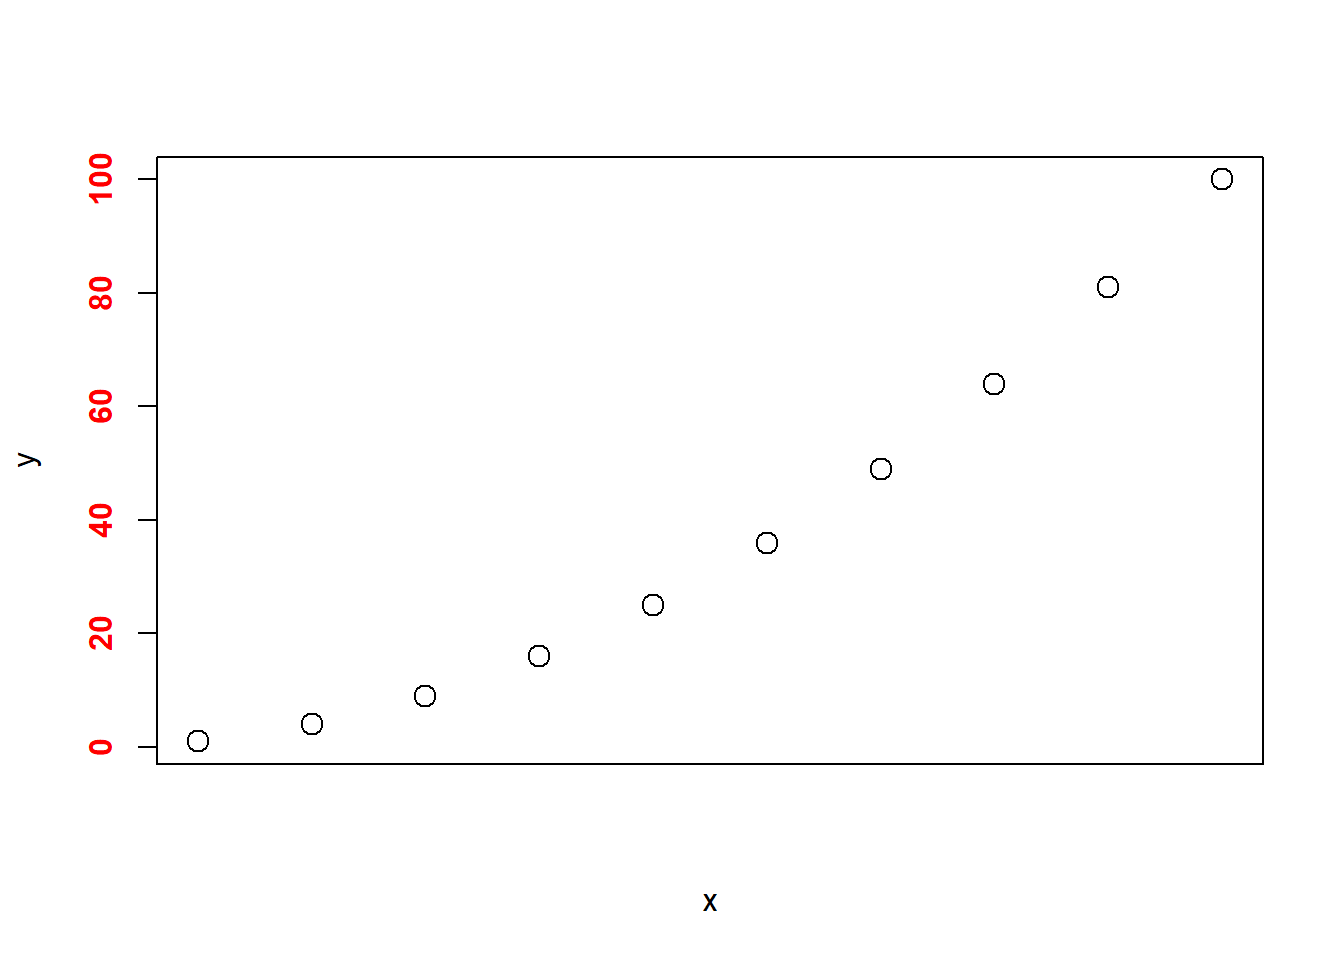
\includegraphics[width=0.7\linewidth]{Metode_Numerik_files/figure-latex/axis3-1} 

}

\caption{Kustomisasi tick mark}\label{fig:axis3}
\end{figure}

\hypertarget{changecolor}{%
\subsection{Mengatur Warna}\label{changecolor}}

Pada fungsi dasar \texttt{R}, warna dapat diatur dengan mengetikkan nama warna maupun kode hexadesimal. Selain itu kita juga dapat menamambahkan warna lain melalui library lain yang tidak dijelaskan pada chapter ini.

Untuk penggunaan warna hexadesima kita perlu mengetikkan ``\#'' yang diukuti oleh 6 kode warna. Untuk memperlajari kode-kode dan warna yang dihasilkan, silahkan pembaca mengunjungi situs \url{http://www.visibone.com/}.

Pada sintaks berikut disajikan visualisasi nama-nama warna bawaan yang ada pada \texttt{R}. Output yang dihasilkan disajikan pada Gambar \ref{fig:color}:

\begin{Shaded}
\begin{Highlighting}[]
\NormalTok{showCols }\OtherTok{\textless{}{-}} \ControlFlowTok{function}\NormalTok{(}\AttributeTok{cl=}\FunctionTok{colors}\NormalTok{(), }\AttributeTok{bg =} \StringTok{"grey"}\NormalTok{,}
                     \AttributeTok{cex =} \FloatTok{0.75}\NormalTok{, }\AttributeTok{rot =} \DecValTok{30}\NormalTok{) \{}
\NormalTok{    m }\OtherTok{\textless{}{-}} \FunctionTok{ceiling}\NormalTok{(}\FunctionTok{sqrt}\NormalTok{(n }\OtherTok{\textless{}{-}}\FunctionTok{length}\NormalTok{(cl)))}
    \FunctionTok{length}\NormalTok{(cl) }\OtherTok{\textless{}{-}}\NormalTok{ m}\SpecialCharTok{*}\NormalTok{m; cm }\OtherTok{\textless{}{-}} \FunctionTok{matrix}\NormalTok{(cl, m)}
    \FunctionTok{require}\NormalTok{(}\StringTok{"grid"}\NormalTok{)}
    \FunctionTok{grid.newpage}\NormalTok{(); vp }\OtherTok{\textless{}{-}} \FunctionTok{viewport}\NormalTok{(}\AttributeTok{w =}\NormalTok{ .}\DecValTok{92}\NormalTok{, }\AttributeTok{h =}\NormalTok{ .}\DecValTok{92}\NormalTok{)}
    \FunctionTok{grid.rect}\NormalTok{(}\AttributeTok{gp=}\FunctionTok{gpar}\NormalTok{(}\AttributeTok{fill=}\NormalTok{bg))}
    \FunctionTok{grid.text}\NormalTok{(cm, }\AttributeTok{x =} \FunctionTok{col}\NormalTok{(cm)}\SpecialCharTok{/}\NormalTok{m, }\AttributeTok{y =} \FunctionTok{rev}\NormalTok{(}\FunctionTok{row}\NormalTok{(cm))}\SpecialCharTok{/}\NormalTok{m, }\AttributeTok{rot =}\NormalTok{ rot,}
              \AttributeTok{vp=}\NormalTok{vp, }\AttributeTok{gp=}\FunctionTok{gpar}\NormalTok{(}\AttributeTok{cex =}\NormalTok{ cex, }\AttributeTok{col =}\NormalTok{ cm))}
\NormalTok{\}}

\CommentTok{\# print 60 nama warna pertama}
\FunctionTok{showCols}\NormalTok{(}\AttributeTok{bg=}\StringTok{"gray20"}\NormalTok{, }\AttributeTok{cl=}\FunctionTok{colors}\NormalTok{()[}\DecValTok{1}\SpecialCharTok{:}\DecValTok{60}\NormalTok{], }\AttributeTok{rot=}\DecValTok{30}\NormalTok{, }\AttributeTok{cex=}\FloatTok{0.9}\NormalTok{)}
\end{Highlighting}
\end{Shaded}

\begin{verbatim}
## Loading required package: grid
\end{verbatim}

\begin{figure}

{\centering 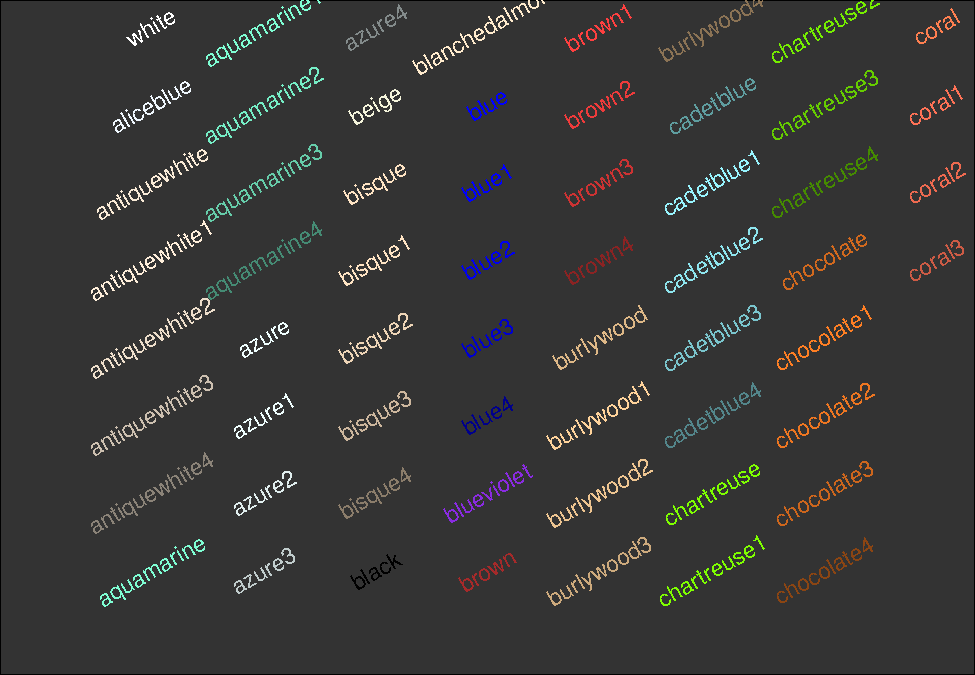
\includegraphics[width=0.7\linewidth]{Metode_Numerik_files/figure-latex/color-1} 

}

\caption{Nama warna}\label{fig:color}
\end{figure}

\hypertarget{plot-dua-dan-tiga-dimensi}{%
\section{Plot Dua dan Tiga Dimensi}\label{plot-dua-dan-tiga-dimensi}}

\texttt{R} dapat digunakan untuk memproduksi visualisasi pada skala 2 dan 3 dimensi. Untuk proyeksi 2 dimensi, fungsi yang digunakan adalah \texttt{image()} atau \texttt{contour()}. Untuk informasi lebih lanjut terkait fungsi tersebut pembaca dapat mengakses menu bantuan. Pada sintak berikut diberikan contoh bagaimana cara memproduksi visualisasi dua dimensi menggunakan kedua fungsi tersebut:

\begin{Shaded}
\begin{Highlighting}[]
\NormalTok{n }\OtherTok{\textless{}{-}} \DecValTok{1}\SpecialCharTok{:}\DecValTok{20}
\NormalTok{x }\OtherTok{\textless{}{-}} \FunctionTok{sin}\NormalTok{(n)}
\NormalTok{y }\OtherTok{\textless{}{-}} \FunctionTok{cos}\NormalTok{(n)}\SpecialCharTok{*}\FunctionTok{exp}\NormalTok{(}\SpecialCharTok{{-}}\NormalTok{n}\SpecialCharTok{/}\DecValTok{3}\NormalTok{)}
\NormalTok{z }\OtherTok{\textless{}{-}} \FunctionTok{outer}\NormalTok{(x,y)}
\FunctionTok{par}\NormalTok{(}\AttributeTok{mar=}\FunctionTok{c}\NormalTok{(}\DecValTok{3}\NormalTok{,}\DecValTok{3}\NormalTok{,}\FloatTok{1.5}\NormalTok{,}\FloatTok{1.5}\NormalTok{), }\AttributeTok{mex=}\FloatTok{0.8}\NormalTok{, }\AttributeTok{mgp=}\FunctionTok{c}\NormalTok{(}\DecValTok{2}\NormalTok{,}\FloatTok{0.5}\NormalTok{,}\DecValTok{0}\NormalTok{), }\AttributeTok{tcl=}\FloatTok{0.3}\NormalTok{)}
\FunctionTok{par}\NormalTok{(}\AttributeTok{mfrow=}\FunctionTok{c}\NormalTok{(}\DecValTok{1}\NormalTok{,}\DecValTok{2}\NormalTok{))}

\CommentTok{\# plot pertama}
\FunctionTok{image}\NormalTok{(z, }\AttributeTok{col=}\FunctionTok{gray}\NormalTok{(}\DecValTok{1}\SpecialCharTok{:}\DecValTok{10}\SpecialCharTok{/}\DecValTok{10}\NormalTok{))}

\CommentTok{\# plot kedua}
\FunctionTok{contour}\NormalTok{(z)}
\end{Highlighting}
\end{Shaded}

\begin{figure}

{\centering 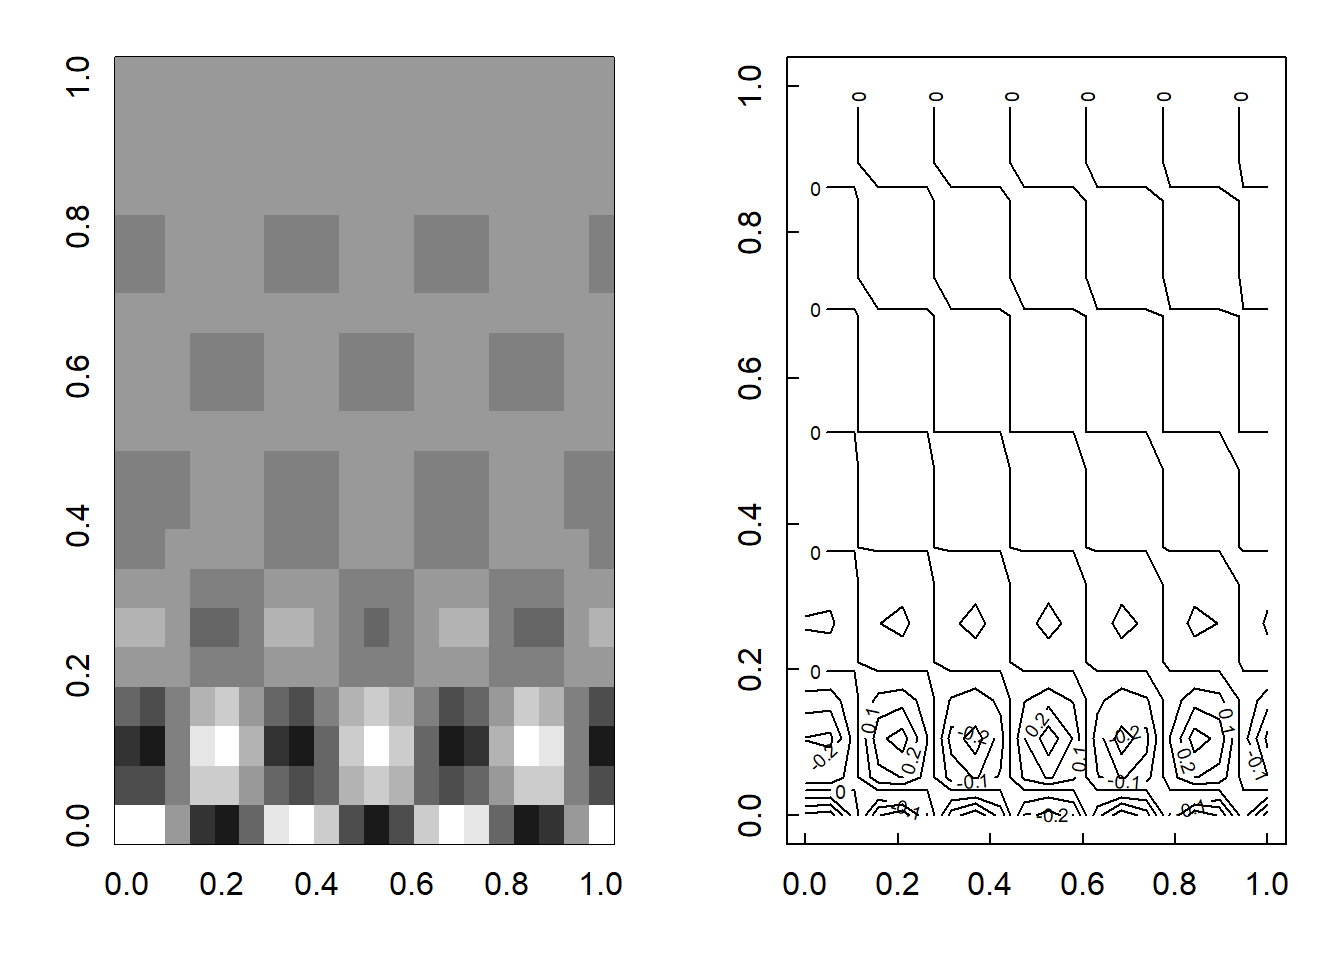
\includegraphics[width=0.8\linewidth]{Metode_Numerik_files/figure-latex/map-1} 

}

\caption{image plot (kiri) dan contour plot (kanan)}\label{fig:map}
\end{figure}

\begin{Shaded}
\begin{Highlighting}[]
\FunctionTok{par}\NormalTok{(}\AttributeTok{mfrow=}\FunctionTok{c}\NormalTok{(}\DecValTok{1}\NormalTok{,}\DecValTok{1}\NormalTok{))}
\end{Highlighting}
\end{Shaded}

Proyeksi 3 dimensi dapat dilakukan menggunakan fungsi \texttt{persp()}. Sudut penglihatan dapat diatur melalui argumen\texttt{theta} (sudut) dan \texttt{phi()} (rotasi). Sintaks berikut merupakan contoh bagaimana cara menghasilkan visualisasi 3 dimensi dari data yang telah diproduksi sebelumnya:

\begin{Shaded}
\begin{Highlighting}[]
\FunctionTok{par}\NormalTok{(}\AttributeTok{mar=}\FunctionTok{c}\NormalTok{(}\DecValTok{3}\NormalTok{,}\DecValTok{3}\NormalTok{,}\FloatTok{1.5}\NormalTok{,}\FloatTok{1.5}\NormalTok{), }\AttributeTok{mex=}\FloatTok{0.8}\NormalTok{, }\AttributeTok{mgp=}\FunctionTok{c}\NormalTok{(}\DecValTok{2}\NormalTok{,}\FloatTok{0.5}\NormalTok{,}\DecValTok{0}\NormalTok{), }\AttributeTok{tcl=}\FloatTok{0.3}\NormalTok{)}
\FunctionTok{par}\NormalTok{(}\AttributeTok{mfrow=}\FunctionTok{c}\NormalTok{(}\DecValTok{1}\NormalTok{,}\DecValTok{2}\NormalTok{))}

\CommentTok{\# plot pertama}
\FunctionTok{persp}\NormalTok{(n,n,z, }\AttributeTok{theta=}\DecValTok{45}\NormalTok{, }\AttributeTok{phi=}\DecValTok{20}\NormalTok{)}

\CommentTok{\# plot kedua}
\FunctionTok{persp}\NormalTok{(n,n,z, }\AttributeTok{theta=}\DecValTok{45}\NormalTok{, }\AttributeTok{phi=}\DecValTok{20}\NormalTok{, }\AttributeTok{shade=}\FloatTok{0.5}\NormalTok{)}
\end{Highlighting}
\end{Shaded}

\begin{figure}

{\centering 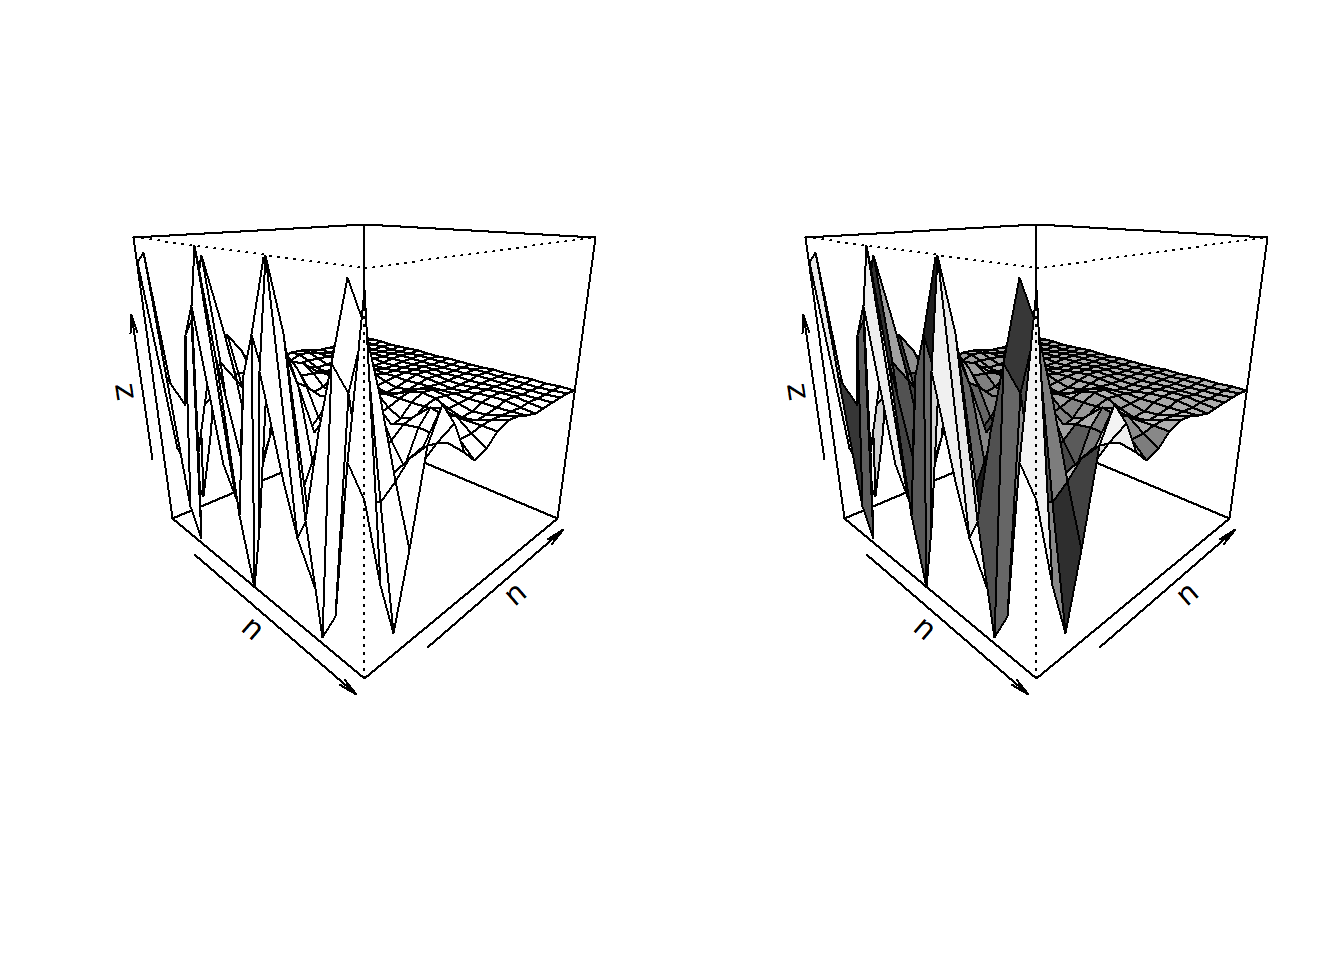
\includegraphics[width=0.8\linewidth]{Metode_Numerik_files/figure-latex/persp-1} 

}

\caption{proyeksi 3 dimensi (kanan) dan proyeksi 3 dimensi dengan pewarnaan}\label{fig:persp}
\end{figure}

\begin{Shaded}
\begin{Highlighting}[]
\FunctionTok{par}\NormalTok{(}\AttributeTok{mfrow=}\FunctionTok{c}\NormalTok{(}\DecValTok{1}\NormalTok{,}\DecValTok{1}\NormalTok{))}
\end{Highlighting}
\end{Shaded}

\hypertarget{referensi-2}{%
\section{Referensi}\label{referensi-2}}

\begin{enumerate}
\def\labelenumi{\arabic{enumi}.}
\tightlist
\item
  Maindonald, J.H. 2008. \textbf{Using R for Data Analysis and Graphics Introduction, Code and Commentary}. Centre for Mathematics and Its Applications Australian National University.
\item
  Scherber, C. 2007. \textbf{An introduction to statistical data analysis using R}. R\_Manual Goettingen.
\item
  STHDA. \textbf{R Base Graphs}. \url{http://www.sthda.com/english/wiki/r-base-graphs}
\item
  Venables, W.N. Smith D.M. and R Core Team. 2018. \textbf{An Introduction to R}. R Manuals.
\end{enumerate}

\hypertarget{programmingandfunction}{%
\chapter{Pemrograman dan Fungsi}\label{programmingandfunction}}

Kita telah membahas dasar-dasar kalkulasi menggunakan \texttt{R} pada Chapter \ref{calculation}. Pada Chapter \ref{programmingandfunction} kita akan membahas dasar pemrograman menggunakan \texttt{R}. Pada chapter ini kita juga akan membahas bagaimana kita dapat membentuk suatu fungsi menggunakan \texttt{R} untuk pekerjaan yang berulang-ulang.

\hypertarget{loop}{%
\section{Loop}\label{loop}}

\emph{Loop} merupakan kode program yang berulang-ulang. \emph{Loop} berguna saat kita ingin melakukan sebuah perintah yang perlu dijalankan berulang-ulang seperti melakukan perhitungan maupaun melakukan visualisasi terhadap banyak variabel secara serentak. Hal ini tentu saja membantu kita karena kita tidak perlu menulis sejumlah sintaks yang berulang-ulang. Kita hanya perlu mengatur \emph{statement} berdasarkan hasil yang kita harapkan.

Pada \texttt{R} bentuk \emph{loop} dapat bermacam-macam (``\emph{for loop}'',``\emph{while loop}'', dll). \texttt{R} menyederhanakan bentuk \emph{loop} ini dengan menyediakan sejumlah fungsi seperti \texttt{apply()},\texttt{tapply()}, dll. Sehingga \texttt{loop} jarang sekali muncul dalam kode \texttt{R}. Sehingga \texttt{R} sering disebut sebagai \emph{loopless loop}.

Meski \emph{loop} jarang muncul bukan berarti kita tidak akan melakukannya. Terkadang saat kita melakukan komputasi statistik atau matematik dan belum terdapat \emph{library} yang mendukung proses tersebut, sering kali kita akan membuat sintaks sendiri berdasarkan algoritma metode tersebut. Pada algoritma tersebut sering pula terdapat \emph{loop} yang diperlukan selama proses perhitungan. Secara sederhana diagram umum loop ditampilkan pada Gambar \ref{fig:loop}

\begin{figure}

{\centering 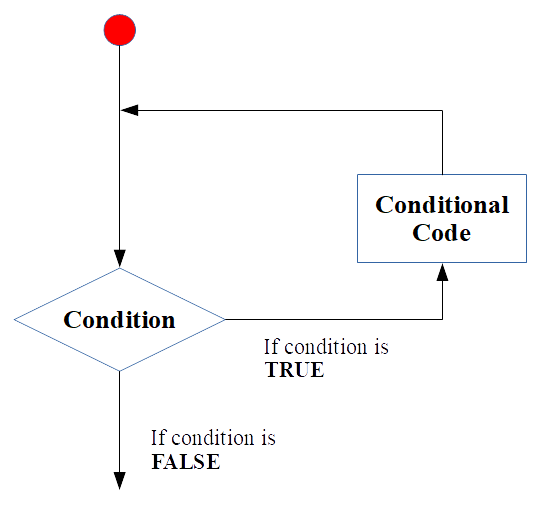
\includegraphics[width=0.4\linewidth]{./images/skema_loop} 

}

\caption{Diagram umum loop (sumber: Primartha, 2018).}\label{fig:loop}
\end{figure}

\hypertarget{forloop}{%
\subsection{For Loop}\label{forloop}}

Mengulangi sebuah \emph{statement} atau sekelompok \emph{statement} sebanyak nilai yang ditentukan di awal. Jadi operasi akan terus dilakukan sampai dengan jumlah yang telah ditetapkan di awal atau dengan kata lain tes kondisi (Jika jumlah pengulangan telah cukup) hanya akan dilakukan di akhir. Secara sederhana bentuk dari \emph{for loop} dapat dituliskan sebagai berikut:

\begin{Shaded}
\begin{Highlighting}[]
\ControlFlowTok{for}\NormalTok{ (value }\ControlFlowTok{in}\NormalTok{ vector)\{}
\NormalTok{  statements}
\NormalTok{\}}
\end{Highlighting}
\end{Shaded}

Berikut adalah contoh sintaks penerapan \emph{for loop}:

\begin{Shaded}
\begin{Highlighting}[]
\CommentTok{\# Membuat vektor numerik}
\NormalTok{vektor }\OtherTok{\textless{}{-}} \FunctionTok{c}\NormalTok{(}\DecValTok{1}\SpecialCharTok{:}\DecValTok{5}\NormalTok{)}

\CommentTok{\# loop }
\ControlFlowTok{for}\NormalTok{(i }\ControlFlowTok{in}\NormalTok{ vektor)\{}
  \FunctionTok{print}\NormalTok{(i)}
\NormalTok{\}}
\end{Highlighting}
\end{Shaded}

\begin{verbatim}
## [1] 1
## [1] 2
## [1] 3
## [1] 4
## [1] 5
\end{verbatim}

\emph{Loop} akan dimulai dari blok \emph{statement for} sampai dengan \texttt{print(i)}. Berdasarkan \emph{loop} pada contoh tersebut, \emph{loop} hanya dilakukan sebanyak 5 kali sesuai dengan jumlah vektor yang ada.

\hypertarget{whileloop}{%
\subsection{While Loop}\label{whileloop}}

\emph{While loop} merupakan loop yang digunakan ketika kita telah menetapkan \emph{stop condition} sebelumnya. Blok \emph{statement}/kode yang sama akan terus dijalankan sampai \emph{stop condition} ini tercapai. \emph{Stop condition} akan di cek sebelum melakukan proses \emph{loop}. Berikut adalah pola dari \emph{while loop} dapat dituliskan sebagai berikut:

\begin{Shaded}
\begin{Highlighting}[]
\ControlFlowTok{while}\NormalTok{ (test\_expression)\{}
\NormalTok{  statement}
\NormalTok{\}}
\end{Highlighting}
\end{Shaded}

Berikut adalah contoh penerapan dari \emph{while loop}:

\begin{Shaded}
\begin{Highlighting}[]
\NormalTok{coba }\OtherTok{\textless{}{-}} \FunctionTok{c}\NormalTok{(}\StringTok{"Contoh"}\NormalTok{)}
\NormalTok{counter }\OtherTok{\textless{}{-}} \DecValTok{1}

\CommentTok{\# loop}
\ControlFlowTok{while}\NormalTok{ (counter}\SpecialCharTok{\textless{}}\DecValTok{5}\NormalTok{)\{}
  \CommentTok{\# print vektor}
  \FunctionTok{print}\NormalTok{(coba)}
  \CommentTok{\# tambahkan nilai counter sehingga proses terus berlangsung sampai counter = 5 }
\NormalTok{  counter }\OtherTok{\textless{}{-}}\NormalTok{ counter }\SpecialCharTok{+} \DecValTok{1}
\NormalTok{\}}
\end{Highlighting}
\end{Shaded}

\begin{verbatim}
## [1] "Contoh"
## [1] "Contoh"
## [1] "Contoh"
## [1] "Contoh"
\end{verbatim}

\emph{Loop} akan dimulai dari blok \emph{statement while} sampai dengan \emph{counter} \textless- 1. \emph{Loop} hanya akan dilakukan sepanjang nilai \emph{counter} \textless{} 5.

\hypertarget{repeatloop}{%
\subsection{Repeat Loop}\label{repeatloop}}

\emph{Repeat loop} akan menjalankan \emph{statement}/kode yang sama berulang-ulang hingga \emph{stop condition} tercapai. Berikut adalah pola dari \emph{repeat loop}.

\begin{Shaded}
\begin{Highlighting}[]
\ControlFlowTok{repeat}\NormalTok{ \{}
\NormalTok{  commands}
  \ControlFlowTok{if}\NormalTok{(condition)\{}
    \ControlFlowTok{break}
\NormalTok{  \}}
\NormalTok{\}}
\end{Highlighting}
\end{Shaded}

Berikut adalah contoh penerapan dari \emph{repeat loop}:

\begin{Shaded}
\begin{Highlighting}[]
\NormalTok{coba }\OtherTok{\textless{}{-}} \FunctionTok{c}\NormalTok{(}\StringTok{"contoh"}\NormalTok{)}
\NormalTok{counter }\OtherTok{\textless{}{-}} \DecValTok{1}
\ControlFlowTok{repeat}\NormalTok{ \{}
  \FunctionTok{print}\NormalTok{(coba)}
\NormalTok{  counter }\OtherTok{\textless{}{-}}\NormalTok{ counter }\SpecialCharTok{+} \DecValTok{1}
  \ControlFlowTok{if}\NormalTok{(counter }\SpecialCharTok{\textless{}} \DecValTok{5}\NormalTok{)\{}
\ControlFlowTok{break}
\NormalTok{  \}}
\NormalTok{\}}
\end{Highlighting}
\end{Shaded}

\begin{verbatim}
## [1] "contoh"
\end{verbatim}

\emph{Loop} akan dimulai dari blok \emph{statement while} sampai dengan \emph{break}. \emph{Loop} hanya akan dilakukan sepanjang nilai \emph{counter} \textless{} 5. Hasil yang diperoleh berbeda dengan \emph{while loop}, dimana kita memperoleh 4 buah kata ``contoh''. Hal ini disebabkan karena \emph{repeat loop} melakukan pengecekan \emph{stop condition} tidak di awal loop seperti \emph{while loop} sehingga berapapun nilainya, selama nilainya sesuai dengan \emph{stop condition} maka \emph{loop} akan dihentikan. Hal ini berbeda dengan \emph{while loop} dimana proses dilakukan berulang-ulang sampai jumlahnya mendekati \emph{stop condition}.

\hypertarget{break}{%
\subsection{Break}\label{break}}

\emph{Break} sebenarnya bukan bagian dari \emph{loop}, namun sering digunakan dalam \emph{loop}. \emph{Break} dapat digunakan pada \emph{loop} manakala dirasa perlu, yaitu saat kondisi yang disyaratkan pada \emph{break} tercapai.

Berikut adalah contoh penerapan \emph{break} pada beberapa jenis \emph{loop}.

\begin{Shaded}
\begin{Highlighting}[]
\CommentTok{\# for loop}
\NormalTok{a }\OtherTok{=} \FunctionTok{c}\NormalTok{(}\DecValTok{2}\NormalTok{,}\DecValTok{4}\NormalTok{,}\DecValTok{6}\NormalTok{,}\DecValTok{8}\NormalTok{,}\DecValTok{10}\NormalTok{,}\DecValTok{12}\NormalTok{,}\DecValTok{14}\NormalTok{)}
\ControlFlowTok{for}\NormalTok{(i }\ControlFlowTok{in}\NormalTok{ a)\{}
  \ControlFlowTok{if}\NormalTok{(i}\SpecialCharTok{\textgreater{}}\DecValTok{8}\NormalTok{)\{}
    \ControlFlowTok{break}
\NormalTok{  \}}
  \FunctionTok{print}\NormalTok{(i)}
\NormalTok{\}}
\end{Highlighting}
\end{Shaded}

\begin{verbatim}
## [1] 2
## [1] 4
## [1] 6
## [1] 8
\end{verbatim}

\begin{Shaded}
\begin{Highlighting}[]
\CommentTok{\# while loop}
\NormalTok{a }\OtherTok{=} \DecValTok{2}
\NormalTok{b }\OtherTok{=} \DecValTok{4}
\ControlFlowTok{while}\NormalTok{(a}\SpecialCharTok{\textless{}}\DecValTok{7}\NormalTok{)\{}
  \FunctionTok{print}\NormalTok{(a)}
\NormalTok{  a }\OtherTok{=}\NormalTok{ a }\SpecialCharTok{+}\DecValTok{1}
  \ControlFlowTok{if}\NormalTok{(b}\SpecialCharTok{+}\NormalTok{a}\SpecialCharTok{\textgreater{}}\DecValTok{10}\NormalTok{)\{}
    \ControlFlowTok{break}
\NormalTok{  \}}
\NormalTok{\}}
\end{Highlighting}
\end{Shaded}

\begin{verbatim}
## [1] 2
## [1] 3
## [1] 4
## [1] 5
## [1] 6
\end{verbatim}

\begin{Shaded}
\begin{Highlighting}[]
\CommentTok{\# repeat loop}
\NormalTok{a }\OtherTok{=} \DecValTok{1}
\ControlFlowTok{repeat}\NormalTok{\{}
  \FunctionTok{print}\NormalTok{(a)}
\NormalTok{  a }\OtherTok{=}\NormalTok{ a}\SpecialCharTok{+}\DecValTok{1}
  \ControlFlowTok{if}\NormalTok{(a}\SpecialCharTok{\textgreater{}}\DecValTok{6}\NormalTok{)\{}
    \ControlFlowTok{break}
\NormalTok{  \}}
\NormalTok{\}}
\end{Highlighting}
\end{Shaded}

\begin{verbatim}
## [1] 1
## [1] 2
## [1] 3
## [1] 4
## [1] 5
## [1] 6
\end{verbatim}

\hypertarget{loopapply}{%
\section{Loop Menggunakan Apply Family Function}\label{loopapply}}

Penggunaan loop sangat membantu kita dalam melakukan proses perhitungan berulang. Namun, metode ini tidak cukup ringkas dalam penerapannya dan perlu penulisan sintaks yang cukup panjang untuk menyelesaikan sebuah kasus yang kita inginkan. Berikut adalah sebuah sintaks yang digunakan untuk menghitung nilai mean pada suatu dataset:

\begin{Shaded}
\begin{Highlighting}[]
\CommentTok{\# subset data iris}
\NormalTok{sub\_iris }\OtherTok{\textless{}{-}}\NormalTok{ iris[,}\SpecialCharTok{{-}}\DecValTok{5}\NormalTok{]}
\CommentTok{\# membuat vektor untuk menyimpan hasil loop}
\NormalTok{a }\OtherTok{\textless{}{-}} \FunctionTok{rep}\NormalTok{(}\ConstantTok{NA}\NormalTok{,}\DecValTok{4}\NormalTok{)}
\CommentTok{\# loop}
\ControlFlowTok{for}\NormalTok{(i }\ControlFlowTok{in} \DecValTok{1}\SpecialCharTok{:}\FunctionTok{length}\NormalTok{(sub\_iris))\{}
\NormalTok{  a[i]}\OtherTok{\textless{}{-}}\FunctionTok{mean}\NormalTok{(sub\_iris[,i])}
\NormalTok{\}}
\CommentTok{\# print}
\NormalTok{a}
\end{Highlighting}
\end{Shaded}

\begin{verbatim}
## [1] 5.843 3.057 3.758 1.199
\end{verbatim}

\begin{Shaded}
\begin{Highlighting}[]
\FunctionTok{class}\NormalTok{(a) }\CommentTok{\# cek kelas objek}
\end{Highlighting}
\end{Shaded}

\begin{verbatim}
## [1] "numeric"
\end{verbatim}

Metode alternatif lain untuk melakukan loop suatu fungsi adalah dengan menggunakan Apply function family. Metode ini memungkinkan kita untuk melakukan loop suatu fungsi tanpa perlu menuliskan sintaks loop. Berikut adalah beberapa fungsi dari apply family yang nantinya akan sering kita gunakan:

\begin{itemize}
\tightlist
\item
  \texttt{apply()}: fungsi generik yang mengaplikasikan fungsi kepada kolom atau baris pada matriks atau secara lebih general aplikasi dilakukan pada dimensi untuk jenis data array.
\item
  \texttt{lapply()}: fungsi apply yang bekerja pada jenis data list dan memberikan output berupa list juga.
\item
  \texttt{sapply()}: bentuk sederhana dari lapply yang menghasilkan output berupa matriks atau vektor.
\item
  \texttt{vapply()}: disebut juga \emph{verified apply} (memungkinkan untuk menghasilkan output dengan jenis data yang telah ditentukan sebelumnya).
\item
  \texttt{tapply()}: \emph{tagged apply} dimana dimana tag menentukan subset dari data.
\end{itemize}

\hypertarget{apply}{%
\subsection{Apply}\label{apply}}

Fungsi \texttt{apply()} bekerja dengan jenis data matrik atau array (jenis data homogen). Kita dapat melakukan spesifikasi apakah suatu fungsi hanya akan bekerja pada kolom saja, baris saja atau keduanya. Format fungsi ini adalah sebagai berikut:

\begin{Shaded}
\begin{Highlighting}[]
\FunctionTok{apply}\NormalTok{(X, MARGIN, FUN, ...)}
\end{Highlighting}
\end{Shaded}

\begin{quote}
\textbf{Catatan:}

\begin{itemize}
\tightlist
\item
  \textbf{X}: matriks atau array
\item
  \textbf{MARGIN}: menentukan bagaimana fungsi bekerja terhadap matriks atau array. Jika nilai yang diinputkan 1, maka fungsi akan bekerja pada masing-masing baris pada matriks. Jika nilainya 2, maka fungsi akan bekerja pada tiap kolom pada matriks.
\item
  \textbf{FUN}: fungsi yang akan digunakan. Fungsi yang dapat digunakan dapat berupa fungsi dasar matematika atau statistika, serta user define function.
\item
  \textbf{\ldots{}}: opsional argumen pada fungsi yang digunakan.
\end{itemize}
\end{quote}

Berikut adalah contoh bagaimana aplikasi fungsi tersebut pada matriks:

\begin{Shaded}
\begin{Highlighting}[]
\DocumentationTok{\#\# membuat matriks}
\NormalTok{x }\OtherTok{\textless{}{-}} \FunctionTok{cbind}\NormalTok{(}\AttributeTok{x1 =} \DecValTok{3}\NormalTok{, }\AttributeTok{x2 =} \FunctionTok{c}\NormalTok{(}\DecValTok{4}\SpecialCharTok{:}\DecValTok{1}\NormalTok{, }\DecValTok{2}\SpecialCharTok{:}\DecValTok{5}\NormalTok{))}
\NormalTok{x }\CommentTok{\# print}
\end{Highlighting}
\end{Shaded}

\begin{verbatim}
##      x1 x2
## [1,]  3  4
## [2,]  3  3
## [3,]  3  2
## [4,]  3  1
## [5,]  3  2
## [6,]  3  3
## [7,]  3  4
## [8,]  3  5
\end{verbatim}

\begin{Shaded}
\begin{Highlighting}[]
\FunctionTok{class}\NormalTok{(x) }\CommentTok{\# cek kelas objek}
\end{Highlighting}
\end{Shaded}

\begin{verbatim}
## [1] "matrix" "array"
\end{verbatim}

\begin{Shaded}
\begin{Highlighting}[]
\DocumentationTok{\#\# menghitung mean masing{-}masing kolom}
\FunctionTok{apply}\NormalTok{(x, }\AttributeTok{MARGIN=}\DecValTok{2}\NormalTok{ ,}\AttributeTok{FUN=}\NormalTok{mean, }\AttributeTok{trim=}\FloatTok{0.2}\NormalTok{, }\AttributeTok{na.rm=}\ConstantTok{TRUE}\NormalTok{)}
\end{Highlighting}
\end{Shaded}

\begin{verbatim}
## x1 x2 
##  3  3
\end{verbatim}

\begin{Shaded}
\begin{Highlighting}[]
\DocumentationTok{\#\# menghitung range pada masing{-}masing baris}
\DocumentationTok{\#\# menggunakan user define function}
\FunctionTok{apply}\NormalTok{(x, }\AttributeTok{MARGIN=}\DecValTok{1}\NormalTok{,}
      \AttributeTok{FUN=}\ControlFlowTok{function}\NormalTok{(x)\{}
        \FunctionTok{max}\NormalTok{(x)}\SpecialCharTok{{-}}\FunctionTok{min}\NormalTok{(x)}
\NormalTok{      \})}
\end{Highlighting}
\end{Shaded}

\begin{verbatim}
## [1] 1 0 1 2 1 0 1 2
\end{verbatim}

\hypertarget{lapply}{%
\subsection{lapply}\label{lapply}}

Fungsi ini melakukan loop fungsi terhadap input data berupa list. Output yang dihasilkan juga merupakan list dengan panjang list yang sama dengan yang diinputkan. Format yang digunakan adalah sebagai berikut:

\begin{Shaded}
\begin{Highlighting}[]
\FunctionTok{lapply}\NormalTok{(X, FUN, ...)}
\end{Highlighting}
\end{Shaded}

\begin{quote}
\textbf{Catatan:}

\begin{itemize}
\tightlist
\item
  \textbf{X}: vektor, data frame atau list
\item
  \textbf{FUN}: fungsi yang akan digunakan. Fungsi yang dapat digunakan dapat berupa fungsi dasar matematika atau statistika, serta user define function. Subset juga dimungkinkan pada fungsi ini.
\item
  \textbf{\ldots{}}: opsional argumen pada fungsi yang digunakan.
\end{itemize}
\end{quote}

Berikut adalah contoh penerapan fungsi lapply:

\begin{Shaded}
\begin{Highlighting}[]
\DocumentationTok{\#\# Membuat list}
\NormalTok{x }\OtherTok{\textless{}{-}} \FunctionTok{list}\NormalTok{(}\AttributeTok{a =} \DecValTok{1}\SpecialCharTok{:}\DecValTok{10}\NormalTok{, }\AttributeTok{beta =} \FunctionTok{exp}\NormalTok{(}\SpecialCharTok{{-}}\DecValTok{3}\SpecialCharTok{:}\DecValTok{3}\NormalTok{), }\AttributeTok{logic =} \FunctionTok{c}\NormalTok{(}\ConstantTok{TRUE}\NormalTok{,}\ConstantTok{FALSE}\NormalTok{,}\ConstantTok{FALSE}\NormalTok{,}\ConstantTok{TRUE}\NormalTok{))}
\NormalTok{x }\CommentTok{\# print}
\end{Highlighting}
\end{Shaded}

\begin{verbatim}
## $a
##  [1]  1  2  3  4  5  6  7  8  9 10
## 
## $beta
## [1]  0.04979  0.13534  0.36788  1.00000  2.71828
## [6]  7.38906 20.08554
## 
## $logic
## [1]  TRUE FALSE FALSE  TRUE
\end{verbatim}

\begin{Shaded}
\begin{Highlighting}[]
\FunctionTok{class}\NormalTok{(x) }\CommentTok{\# cek kelas objek}
\end{Highlighting}
\end{Shaded}

\begin{verbatim}
## [1] "list"
\end{verbatim}

\begin{Shaded}
\begin{Highlighting}[]
\DocumentationTok{\#\# Menghitung nilai mean pada masing{-}masing baris lits}
\FunctionTok{lapply}\NormalTok{(x, }\AttributeTok{FUN=}\NormalTok{mean)}
\end{Highlighting}
\end{Shaded}

\begin{verbatim}
## $a
## [1] 5.5
## 
## $beta
## [1] 4.535
## 
## $logic
## [1] 0.5
\end{verbatim}

\begin{Shaded}
\begin{Highlighting}[]
\DocumentationTok{\#\# Menghitung mean tiap kolom dataset iris}
\FunctionTok{lapply}\NormalTok{(iris, }\AttributeTok{FUN=}\NormalTok{mean)}
\end{Highlighting}
\end{Shaded}

\begin{verbatim}
## Warning in mean.default(X[[i]], ...): argument is not
## numeric or logical: returning NA
\end{verbatim}

\begin{verbatim}
## $Sepal.Length
## [1] 5.843
## 
## $Sepal.Width
## [1] 3.057
## 
## $Petal.Length
## [1] 3.758
## 
## $Petal.Width
## [1] 1.199
## 
## $Species
## [1] NA
\end{verbatim}

\begin{Shaded}
\begin{Highlighting}[]
\DocumentationTok{\#\# Mengalikan elemen vektor dengan suatu nilai}
\NormalTok{y }\OtherTok{\textless{}{-}} \FunctionTok{c}\NormalTok{(}\DecValTok{1}\SpecialCharTok{:}\DecValTok{5}\NormalTok{)}
\FunctionTok{lapply}\NormalTok{(y, }\AttributeTok{FUN=}\ControlFlowTok{function}\NormalTok{(x)\{x}\SpecialCharTok{*}\DecValTok{5}\NormalTok{\})}
\end{Highlighting}
\end{Shaded}

\begin{verbatim}
## [[1]]
## [1] 5
## 
## [[2]]
## [1] 10
## 
## [[3]]
## [1] 15
## 
## [[4]]
## [1] 20
## 
## [[5]]
## [1] 25
\end{verbatim}

\begin{Shaded}
\begin{Highlighting}[]
\DocumentationTok{\#\# Mengubah output menjadi vektor}
\FunctionTok{unlist}\NormalTok{(}\FunctionTok{lapply}\NormalTok{(y, }\AttributeTok{FUN=}\ControlFlowTok{function}\NormalTok{(x)\{x}\SpecialCharTok{*}\DecValTok{5}\NormalTok{\}))}
\end{Highlighting}
\end{Shaded}

\begin{verbatim}
## [1]  5 10 15 20 25
\end{verbatim}

\hypertarget{sapply}{%
\subsection{sapply}\label{sapply}}

Fungsi \texttt{sapply()} merupakan bentuk lain dari fungsi \texttt{lapply()}. Perbedaanya terletak pada output default yang dihasilkan. Secara default \texttt{sapply()} menerima input utama berupa list (dapat pula dataframe atau vektor), namun tidak seperti \texttt{lapply()} jenis data output yang dihasilkan adalah vektor. Untuk mengubah output menjadi list perlu argumen tambahan berupa \texttt{simplify=FALSE}. Format fungsi tersebut adalah sebagai berikut:

\begin{Shaded}
\begin{Highlighting}[]
\FunctionTok{sapply}\NormalTok{(X, FUN, ..., }\AttributeTok{simplify =} \ConstantTok{TRUE}\NormalTok{, }\AttributeTok{USE.NAMES =} \ConstantTok{TRUE}\NormalTok{)}
\end{Highlighting}
\end{Shaded}

\begin{quote}
\textbf{Catatan:}

\begin{itemize}
\tightlist
\item
  \textbf{X}: vektor, data frame atau list
\item
  \textbf{FUN}: fungsi yang akan digunakan. Fungsi yang dapat digunakan dapat berupa fungsi dasar matematika atau statistika, serta user define function. Subset juga dimungkinkan pada fungsi ini.
\item
  \textbf{\ldots{}}: opsional argumen pada fungsi yang digunakan.
\item
  \textbf{simplify}: logical. Jika nilainya \texttt{TRUE} maka output yang dihasilkan adalah bentuk sederhana dari vektor, matrix atau array.
\item
  \textbf{USE.NAMES}: jika list memiliki nama pada setiap elemennya, maka nama elemen tersebut akan secara default ditampilkan.
\end{itemize}
\end{quote}

Berikut adalah contoh penerapannya:

\begin{Shaded}
\begin{Highlighting}[]
\DocumentationTok{\#\# membuat list}
\NormalTok{x }\OtherTok{\textless{}{-}} \FunctionTok{list}\NormalTok{(}\AttributeTok{a =} \DecValTok{1}\SpecialCharTok{:}\DecValTok{10}\NormalTok{, }\AttributeTok{beta =} \FunctionTok{exp}\NormalTok{(}\SpecialCharTok{{-}}\DecValTok{3}\SpecialCharTok{:}\DecValTok{3}\NormalTok{), }\AttributeTok{logic =} \FunctionTok{c}\NormalTok{(}\ConstantTok{TRUE}\NormalTok{,}\ConstantTok{FALSE}\NormalTok{,}\ConstantTok{FALSE}\NormalTok{,}\ConstantTok{TRUE}\NormalTok{))}

\DocumentationTok{\#\# menghitung nilai mean setiap elemen}
\FunctionTok{sapply}\NormalTok{(x, }\AttributeTok{FUN=}\NormalTok{mean)}
\end{Highlighting}
\end{Shaded}

\begin{verbatim}
##     a  beta logic 
## 5.500 4.535 0.500
\end{verbatim}

\begin{Shaded}
\begin{Highlighting}[]
\DocumentationTok{\#\# menghitung nilai mean dengan output list}
\FunctionTok{sapply}\NormalTok{(x, }\AttributeTok{FUN=}\NormalTok{mean, }\AttributeTok{simplify=}\ConstantTok{FALSE}\NormalTok{)}
\end{Highlighting}
\end{Shaded}

\begin{verbatim}
## $a
## [1] 5.5
## 
## $beta
## [1] 4.535
## 
## $logic
## [1] 0.5
\end{verbatim}

\begin{Shaded}
\begin{Highlighting}[]
\DocumentationTok{\#\# summary objek dataframe}
\FunctionTok{sapply}\NormalTok{(mtcars, }\AttributeTok{FUN=}\NormalTok{summary)}
\end{Highlighting}
\end{Shaded}

\begin{verbatim}
##           mpg   cyl  disp    hp  drat    wt  qsec
## Min.    10.40 4.000  71.1  52.0 2.760 1.513 14.50
## 1st Qu. 15.43 4.000 120.8  96.5 3.080 2.581 16.89
## Median  19.20 6.000 196.3 123.0 3.695 3.325 17.71
## Mean    20.09 6.188 230.7 146.7 3.597 3.217 17.85
## 3rd Qu. 22.80 8.000 326.0 180.0 3.920 3.610 18.90
## Max.    33.90 8.000 472.0 335.0 4.930 5.424 22.90
##             vs     am  gear  carb
## Min.    0.0000 0.0000 3.000 1.000
## 1st Qu. 0.0000 0.0000 3.000 2.000
## Median  0.0000 0.0000 4.000 2.000
## Mean    0.4375 0.4062 3.688 2.812
## 3rd Qu. 1.0000 1.0000 4.000 4.000
## Max.    1.0000 1.0000 5.000 8.000
\end{verbatim}

\begin{Shaded}
\begin{Highlighting}[]
\DocumentationTok{\#\# summary objek list}
\NormalTok{a }\OtherTok{\textless{}{-}} \FunctionTok{list}\NormalTok{(}\AttributeTok{mobil=}\NormalTok{mtcars, }\AttributeTok{anggrek=}\NormalTok{iris)}
\FunctionTok{sapply}\NormalTok{(a, }\AttributeTok{FUN=}\NormalTok{summary)}
\end{Highlighting}
\end{Shaded}

\begin{verbatim}
## $mobil
##       mpg            cyl            disp      
##  Min.   :10.4   Min.   :4.00   Min.   : 71.1  
##  1st Qu.:15.4   1st Qu.:4.00   1st Qu.:120.8  
##  Median :19.2   Median :6.00   Median :196.3  
##  Mean   :20.1   Mean   :6.19   Mean   :230.7  
##  3rd Qu.:22.8   3rd Qu.:8.00   3rd Qu.:326.0  
##  Max.   :33.9   Max.   :8.00   Max.   :472.0  
##        hp             drat            wt      
##  Min.   : 52.0   Min.   :2.76   Min.   :1.51  
##  1st Qu.: 96.5   1st Qu.:3.08   1st Qu.:2.58  
##  Median :123.0   Median :3.69   Median :3.33  
##  Mean   :146.7   Mean   :3.60   Mean   :3.22  
##  3rd Qu.:180.0   3rd Qu.:3.92   3rd Qu.:3.61  
##  Max.   :335.0   Max.   :4.93   Max.   :5.42  
##       qsec            vs              am       
##  Min.   :14.5   Min.   :0.000   Min.   :0.000  
##  1st Qu.:16.9   1st Qu.:0.000   1st Qu.:0.000  
##  Median :17.7   Median :0.000   Median :0.000  
##  Mean   :17.8   Mean   :0.438   Mean   :0.406  
##  3rd Qu.:18.9   3rd Qu.:1.000   3rd Qu.:1.000  
##  Max.   :22.9   Max.   :1.000   Max.   :1.000  
##       gear           carb     
##  Min.   :3.00   Min.   :1.00  
##  1st Qu.:3.00   1st Qu.:2.00  
##  Median :4.00   Median :2.00  
##  Mean   :3.69   Mean   :2.81  
##  3rd Qu.:4.00   3rd Qu.:4.00  
##  Max.   :5.00   Max.   :8.00  
## 
## $anggrek
##   Sepal.Length   Sepal.Width    Petal.Length 
##  Min.   :4.30   Min.   :2.00   Min.   :1.00  
##  1st Qu.:5.10   1st Qu.:2.80   1st Qu.:1.60  
##  Median :5.80   Median :3.00   Median :4.35  
##  Mean   :5.84   Mean   :3.06   Mean   :3.76  
##  3rd Qu.:6.40   3rd Qu.:3.30   3rd Qu.:5.10  
##  Max.   :7.90   Max.   :4.40   Max.   :6.90  
##   Petal.Width        Species  
##  Min.   :0.1   setosa    :50  
##  1st Qu.:0.3   versicolor:50  
##  Median :1.3   virginica :50  
##  Mean   :1.2                  
##  3rd Qu.:1.8                  
##  Max.   :2.5
\end{verbatim}

\hypertarget{vapply}{%
\subsection{vapply}\label{vapply}}

Funsgi ini merupakan bentuk lain dari \texttt{sapply()}. Bedanya secara kecepatan proses fungsi ini lebih cepat dari \texttt{sapply()}. Hal yang menarik dari fungsi ini kita dapat menambahkan argumen \texttt{FUN.VALUE}. pada argumen ini kita memasukkan vektor berupa output fungsi yang diinginkan. Perbedaan lainnya adalah output yang dihasilkan hanya berupa matriks atau array. Format dari fungsi ini adalah sebagai berikut:

\begin{Shaded}
\begin{Highlighting}[]
\FunctionTok{vapply}\NormalTok{(X, FUN, FUN.VALUE, ..., }\AttributeTok{USE.NAMES =} \ConstantTok{TRUE}\NormalTok{)}
\end{Highlighting}
\end{Shaded}

\begin{quote}
\textbf{Catatan:}

\begin{itemize}
\tightlist
\item
  \textbf{X}: vektor, data frame atau list
\item
  \textbf{FUN}: fungsi yang akan digunakan. Fungsi yang dapat digunakan dapat berupa fungsi dasar matematika atau statistika, serta user define function. Subset juga dimungkinkan pada fungsi ini.
\item
  \textbf{FUN.VALUE}: vektor, template dari return value FUN.
\item
  \textbf{\ldots{}}: opsional argumen pada fungsi yang digunakan.
\item
  \textbf{USE.NAMES}: jika list memiliki nama pada setiap elemennya, maka nama elemen tersebut akan secara default ditampilkan.
\end{itemize}
\end{quote}

Berikut adalah contoh penerapannya:

\begin{Shaded}
\begin{Highlighting}[]
\DocumentationTok{\#\# membuat list}
\NormalTok{x }\OtherTok{\textless{}{-}} \FunctionTok{sapply}\NormalTok{(}\DecValTok{3}\SpecialCharTok{:}\DecValTok{9}\NormalTok{, seq)}
\NormalTok{x }\CommentTok{\# print}
\end{Highlighting}
\end{Shaded}

\begin{verbatim}
## [[1]]
## [1] 1 2 3
## 
## [[2]]
## [1] 1 2 3 4
## 
## [[3]]
## [1] 1 2 3 4 5
## 
## [[4]]
## [1] 1 2 3 4 5 6
## 
## [[5]]
## [1] 1 2 3 4 5 6 7
## 
## [[6]]
## [1] 1 2 3 4 5 6 7 8
## 
## [[7]]
## [1] 1 2 3 4 5 6 7 8 9
\end{verbatim}

\begin{Shaded}
\begin{Highlighting}[]
\DocumentationTok{\#\# membuat ringkasan data pada tiap elemen list}
\FunctionTok{vapply}\NormalTok{(x, fivenum,}
       \FunctionTok{c}\NormalTok{(}\AttributeTok{Min. =} \DecValTok{0}\NormalTok{, }\StringTok{"1st Qu."} \OtherTok{=} \DecValTok{0}\NormalTok{, }
         \AttributeTok{Median =} \DecValTok{0}\NormalTok{, }\StringTok{"3rd Qu."} \OtherTok{=} \DecValTok{0}\NormalTok{, }\AttributeTok{Max. =} \DecValTok{0}\NormalTok{))}
\end{Highlighting}
\end{Shaded}

\begin{verbatim}
##         [,1] [,2] [,3] [,4] [,5] [,6] [,7]
## Min.     1.0  1.0    1  1.0  1.0  1.0    1
## 1st Qu.  1.5  1.5    2  2.0  2.5  2.5    3
## Median   2.0  2.5    3  3.5  4.0  4.5    5
## 3rd Qu.  2.5  3.5    4  5.0  5.5  6.5    7
## Max.     3.0  4.0    5  6.0  7.0  8.0    9
\end{verbatim}

\begin{Shaded}
\begin{Highlighting}[]
\DocumentationTok{\#\# membuat ringkasan data pada tiap kolom dataframe}
\FunctionTok{vapply}\NormalTok{(mtcars, summary,}
       \FunctionTok{c}\NormalTok{(}\AttributeTok{Min. =} \DecValTok{0}\NormalTok{, }\StringTok{"1st Qu."} \OtherTok{=} \DecValTok{0}\NormalTok{, }
         \AttributeTok{Median =} \DecValTok{0}\NormalTok{, }\StringTok{"3rd Qu."} \OtherTok{=} \DecValTok{0}\NormalTok{, }\AttributeTok{Max. =} \DecValTok{0}\NormalTok{, }\AttributeTok{Mean=}\DecValTok{0}\NormalTok{))}
\end{Highlighting}
\end{Shaded}

\begin{verbatim}
##           mpg   cyl  disp    hp  drat    wt  qsec
## Min.    10.40 4.000  71.1  52.0 2.760 1.513 14.50
## 1st Qu. 15.43 4.000 120.8  96.5 3.080 2.581 16.89
## Median  19.20 6.000 196.3 123.0 3.695 3.325 17.71
## 3rd Qu. 20.09 6.188 230.7 146.7 3.597 3.217 17.85
## Max.    22.80 8.000 326.0 180.0 3.920 3.610 18.90
## Mean    33.90 8.000 472.0 335.0 4.930 5.424 22.90
##             vs     am  gear  carb
## Min.    0.0000 0.0000 3.000 1.000
## 1st Qu. 0.0000 0.0000 3.000 2.000
## Median  0.0000 0.0000 4.000 2.000
## 3rd Qu. 0.4375 0.4062 3.688 2.812
## Max.    1.0000 1.0000 4.000 4.000
## Mean    1.0000 1.0000 5.000 8.000
\end{verbatim}

\hypertarget{tapply}{%
\subsection{tapply}\label{tapply}}

Fungsi ini sangat berguna jika pembaca ingin menghitung suatu nilai misalnya mean berdasarkan grup data atau factor. Format fungsi ini adalah sebagi berikut:

\begin{Shaded}
\begin{Highlighting}[]
\FunctionTok{tapply}\NormalTok{(X, INDEX, }\AttributeTok{FUN =} \ConstantTok{NULL}\NormalTok{, ..., }\AttributeTok{simplify =} \ConstantTok{TRUE}\NormalTok{)}
\end{Highlighting}
\end{Shaded}

\begin{quote}
\textbf{Catatan:}

\begin{itemize}
\tightlist
\item
  \textbf{X}: vektor, data frame atau list
\item
  \textbf{INDEX}: list satu atau beberapa factor yang memiliki panjang sama dengan X.
\item
  \textbf{FUN}: fungsi yang akan digunakan. Fungsi yang dapat digunakan dapat berupa fungsi dasar matematika atau statistika, serta user define function. Subset juga dimungkinkan pada fungsi ini.
\item
  \textbf{\ldots{}}: opsional argumen pada fungsi yang digunakan.
\item
  \textbf{simplify}: logical. Jika nilainya \texttt{TRUE} maka output yang dihasilkan adalah bentuk skalar.
\end{itemize}
\end{quote}

Berikut adalah contoh penerapannya:

\begin{Shaded}
\begin{Highlighting}[]
\DocumentationTok{\#\# membuat tabel frekuensi}
\NormalTok{groups }\OtherTok{\textless{}{-}} \FunctionTok{as.factor}\NormalTok{(}\FunctionTok{rbinom}\NormalTok{(}\DecValTok{32}\NormalTok{, }\AttributeTok{n =} \DecValTok{5}\NormalTok{, }\AttributeTok{prob =} \FloatTok{0.4}\NormalTok{))}

\FunctionTok{tapply}\NormalTok{(groups, groups, length)}
\end{Highlighting}
\end{Shaded}

\begin{verbatim}
## 12 13 16 
##  2  2  1
\end{verbatim}

\begin{Shaded}
\begin{Highlighting}[]
\CommentTok{\# atau}
\FunctionTok{table}\NormalTok{(groups)}
\end{Highlighting}
\end{Shaded}

\begin{verbatim}
## groups
## 12 13 16 
##  2  2  1
\end{verbatim}

\begin{Shaded}
\begin{Highlighting}[]
\DocumentationTok{\#\# membuat tabel kontingensi}
\CommentTok{\# menghitung jumlah breaks berdasarkan faktor jenis wool}
\CommentTok{\# dan tensi level}
\FunctionTok{tapply}\NormalTok{(}\AttributeTok{X=}\NormalTok{warpbreaks}\SpecialCharTok{$}\NormalTok{breaks, }\AttributeTok{INDEX=}\NormalTok{warpbreaks[,}\SpecialCharTok{{-}}\DecValTok{1}\NormalTok{], }\AttributeTok{FUN=}\NormalTok{sum)}
\end{Highlighting}
\end{Shaded}

\begin{verbatim}
##     tension
## wool   L   M   H
##    A 401 216 221
##    B 254 259 169
\end{verbatim}

\begin{Shaded}
\begin{Highlighting}[]
\CommentTok{\# menghitung mean panjang gigi babi hutan berdasarkan}
\CommentTok{\# jenis suplemen dan dosisnya}
\FunctionTok{tapply}\NormalTok{(ToothGrowth}\SpecialCharTok{$}\NormalTok{len, ToothGrowth[,}\SpecialCharTok{{-}}\DecValTok{1}\NormalTok{], mean)}
\end{Highlighting}
\end{Shaded}

\begin{verbatim}
##     dose
## supp   0.5     1     2
##   OJ 13.23 22.70 26.06
##   VC  7.98 16.77 26.14
\end{verbatim}

\begin{Shaded}
\begin{Highlighting}[]
\CommentTok{\# menghitung mpg minimum berdasarkan jumlah silinder pada mobil}
\FunctionTok{tapply}\NormalTok{(mtcars}\SpecialCharTok{$}\NormalTok{mpg, mtcars}\SpecialCharTok{$}\NormalTok{cyl, min, }\AttributeTok{simplify=}\ConstantTok{FALSE}\NormalTok{)}
\end{Highlighting}
\end{Shaded}

\begin{verbatim}
## $`4`
## [1] 21.4
## 
## $`6`
## [1] 17.8
## 
## $`8`
## [1] 10.4
\end{verbatim}

\hypertarget{dm}{%
\section{Decision Making}\label{dm}}

\emph{Decicion Making} atau sering disebut sebagai \emph{if then else statement} merupakan bentuk percabagan yang digunakan manakala kita ingin agar program dapat melakukan pengujian terhadap syarat kondisi tertentu. Pada Tabel \ref{tab:percabangan} disajikan daftar percabangan yang digunakan pada \texttt{R}.

\begin{longtable}[]{@{}
  >{\raggedright\arraybackslash}p{(\columnwidth - 2\tabcolsep) * \real{0.1586}}
  >{\raggedright\arraybackslash}p{(\columnwidth - 2\tabcolsep) * \real{0.8414}}@{}}
\caption{\label{tab:percabangan} Daftar percabangan pada \texttt{R}.}\tabularnewline
\toprule\noalign{}
\begin{minipage}[b]{\linewidth}\raggedright
\textbf{Statement}
\end{minipage} & \begin{minipage}[b]{\linewidth}\raggedright
\textbf{Keterangan}
\end{minipage} \\
\midrule\noalign{}
\endfirsthead
\toprule\noalign{}
\begin{minipage}[b]{\linewidth}\raggedright
\textbf{Statement}
\end{minipage} & \begin{minipage}[b]{\linewidth}\raggedright
\textbf{Keterangan}
\end{minipage} \\
\midrule\noalign{}
\endhead
\bottomrule\noalign{}
\endlastfoot
\emph{if statement} & \emph{if statement} hanya terdiri atas sebuah ekspresi \emph{Boolean}, dan diikuti satu atau lebih \emph{statement} \\
\emph{if\ldots else statement} & \emph{if else statement} terdiri atas beberapa buah ekspresi \emph{Boolean}. Ekspressi \emph{Boolean} berikutnya akan dijalankan jika ekspresi *Boolan sebelumnya bernilai FALSE \\
\emph{switch statement} & \emph{switch statement} digunakan untuk mengevaluasi sebuah variabel beberapa pilihan \\
\end{longtable}

\hypertarget{ifstatement}{%
\subsection{if statement}\label{ifstatement}}

Pola \emph{if statement} disajikan pada Gambar \ref{fig:ifstatement}

\begin{figure}

{\centering 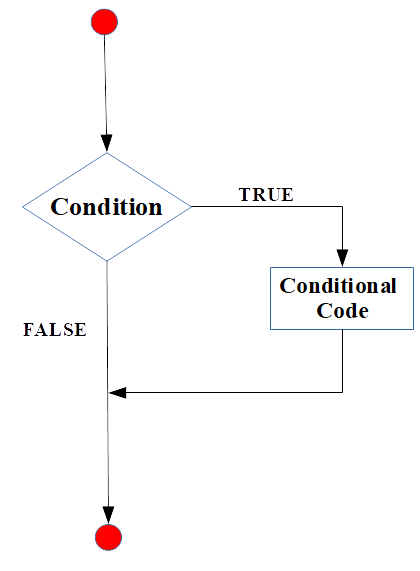
\includegraphics[width=0.4\linewidth]{./images/ifstatement} 

}

\caption{Diagram if statement (sumber: Primartha, 2018).}\label{fig:ifstatement}
\end{figure}

Berikut adalah contoh penerapan \emph{if statement}:

\begin{Shaded}
\begin{Highlighting}[]
\NormalTok{x }\OtherTok{\textless{}{-}} \FunctionTok{c}\NormalTok{(}\DecValTok{1}\SpecialCharTok{:}\DecValTok{5}\NormalTok{)}
\ControlFlowTok{if}\NormalTok{(}\FunctionTok{is.vector}\NormalTok{(x))\{}
  \FunctionTok{print}\NormalTok{(}\StringTok{"x adalah sebuah vector"}\NormalTok{)}
\NormalTok{\}}
\end{Highlighting}
\end{Shaded}

\begin{verbatim}
## [1] "x adalah sebuah vector"
\end{verbatim}

\hypertarget{ifelsestatement}{%
\subsection{if else statement}\label{ifelsestatement}}

Pola dari \emph{if else statement} disajikan pada Gambar \ref{fig:ifelse}

\begin{figure}

{\centering 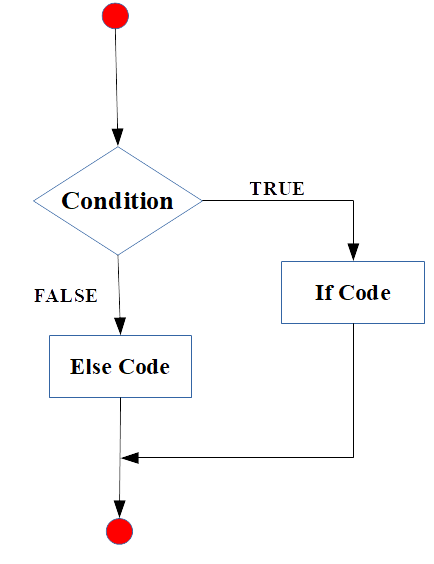
\includegraphics[width=0.4\linewidth]{./images/ifelse} 

}

\caption{Diagram if else statement (sumber: Primartha, 2018).}\label{fig:ifelse}
\end{figure}

Berikut adalah contoh penerapan \emph{if else statement}:

\begin{Shaded}
\begin{Highlighting}[]
\NormalTok{x }\OtherTok{\textless{}{-}} \FunctionTok{c}\NormalTok{(}\StringTok{"Andi"}\NormalTok{,}\StringTok{"Iwan"}\NormalTok{, }\StringTok{"Adi"}\NormalTok{)}
\ControlFlowTok{if}\NormalTok{(}\StringTok{"Rina"} \SpecialCharTok{\%in\%}\NormalTok{ x)\{}
  \FunctionTok{print}\NormalTok{(}\StringTok{"Rina ditemukan"}\NormalTok{)}
\NormalTok{\} }\ControlFlowTok{else} \ControlFlowTok{if}\NormalTok{(}\StringTok{"Adi"} \SpecialCharTok{\%in\%}\NormalTok{ x)\{}
  \FunctionTok{print}\NormalTok{(}\StringTok{"Adi ditemukan"}\NormalTok{)}
\NormalTok{\} }\ControlFlowTok{else}\NormalTok{\{}
  \FunctionTok{print}\NormalTok{(}\StringTok{"tidak ada yang ditemukan"}\NormalTok{)}
\NormalTok{\}}
\end{Highlighting}
\end{Shaded}

\begin{verbatim}
## [1] "Adi ditemukan"
\end{verbatim}

\hypertarget{switchstatement}{%
\subsection{switch statement}\label{switchstatement}}

Pola dari \emph{switch statement} disajikan pada Gambar \ref{fig:switch}

\begin{figure}

{\centering 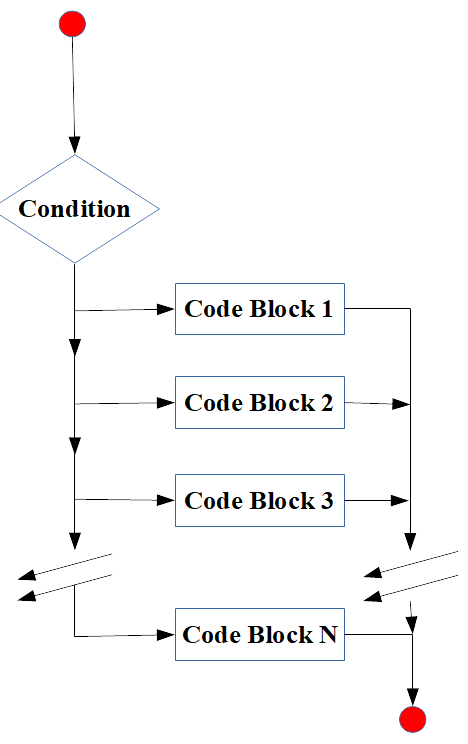
\includegraphics[width=0.4\linewidth]{./images/switch} 

}

\caption{Diagram switch statement (sumber: Primartha, 2018).}\label{fig:switch}
\end{figure}

Berikut adalah contoh penerapan \emph{switch statement}:

\begin{Shaded}
\begin{Highlighting}[]
\NormalTok{y }\OtherTok{=} \DecValTok{3}

\NormalTok{x }\OtherTok{=} \ControlFlowTok{switch}\NormalTok{(}
\NormalTok{  y,}
  \StringTok{"Selamat Pagi"}\NormalTok{,}
  \StringTok{"Selamat Siang"}\NormalTok{,}
  \StringTok{"Selamat Sore"}\NormalTok{,}
  \StringTok{"Selamat Malam"}
\NormalTok{)}

\FunctionTok{print}\NormalTok{(x)}
\end{Highlighting}
\end{Shaded}

\begin{verbatim}
## [1] "Selamat Sore"
\end{verbatim}

\hypertarget{fungsi}{%
\section{Fungsi}\label{fungsi}}

Fungsi merupakan sekumpulan instruksi atau \emph{statement} yang dapat melakukan tugas khusus. Sebagai contoh fungsi perkalian untuk menyelesaikan operasi perkalian, fungsi pemangkatan hanya untuk operasi pemangkatan, dll.

Pada \texttt{R} terdapat 2 jenis fungsi, yaitu: \emph{build in fuction} dan \emph{user define function}. \emph{build in fnction} merupakan fungsi bawaan \texttt{R} saat pertama kita menginstall \texttt{R}. Contohnya adalah \texttt{mean()}, \texttt{sum()}, \texttt{ls()}, \texttt{rm()}, dll. Sedangkan \emph{user define fuction} merupakan fungsi-fungsi yang dibuat sendiri oleh pengguna.

Fungsi-fungsi buatan pengguna haruslah dideklarasikan (dibuat) terlebih dahulu sebelum dapat dijalankan. Pola pembentukan fungsi adalah sebagai berikut:

\begin{Shaded}
\begin{Highlighting}[]
\NormalTok{function\_name }\OtherTok{\textless{}{-}} \ControlFlowTok{function}\NormalTok{(argument\_1, argument\_2, ...)\{}
  \ControlFlowTok{function}\NormalTok{ body}
\NormalTok{\}}
\end{Highlighting}
\end{Shaded}

\begin{quote}
\textbf{Catatan:}

\begin{itemize}
\tightlist
\item
  \textbf{function\_name} : Nama dari fungsi \texttt{R}. \texttt{R} akan menyimpan fungsi tersebut sebagai objek
\item
  \textbf{argument\_1, argument\_2, \ldots{}} : \emph{Argument} bersifat opsional (tidak wajib). \emph{Argument} dapat digunakan untuk memberi inputan kepada fungsi
\item
  \textbf{function body} : Merupakan inti dari fungsi. Fuction body dapat terdiri atas 0 statement (kosong) hingga banyak statement.
\item
  \textbf{return} : Fungsi ada yang memiliki \emph{output} atau \emph{return value} ada juga yang tidak. Jika fungsi memiliki \emph{return value} maka \emph{return value} dapat diproses lebih lanjut
\end{itemize}
\end{quote}

Berikut adalah contoh penerapan \emph{user define function}:

\begin{Shaded}
\begin{Highlighting}[]
\CommentTok{\# Fungsi tanpa argument}
\NormalTok{bilang }\OtherTok{\textless{}{-}} \ControlFlowTok{function}\NormalTok{()\{}
  \FunctionTok{print}\NormalTok{(}\StringTok{"Hello World!!"}\NormalTok{)}
\NormalTok{\}}

\CommentTok{\# Print}
\FunctionTok{bilang}\NormalTok{()}
\end{Highlighting}
\end{Shaded}

\begin{verbatim}
## [1] "Hello World!!"
\end{verbatim}

\begin{Shaded}
\begin{Highlighting}[]
\CommentTok{\# Fungsi dengan argumen}
\NormalTok{tambah }\OtherTok{\textless{}{-}} \ControlFlowTok{function}\NormalTok{(a,b)\{}
  \FunctionTok{print}\NormalTok{(a}\SpecialCharTok{+}\NormalTok{b)}
\NormalTok{\}}

\CommentTok{\# Print}
\FunctionTok{tambah}\NormalTok{(}\DecValTok{5}\NormalTok{,}\DecValTok{3}\NormalTok{)}
\end{Highlighting}
\end{Shaded}

\begin{verbatim}
## [1] 8
\end{verbatim}

\begin{Shaded}
\begin{Highlighting}[]
\CommentTok{\# Fungsi dengan return value}
\NormalTok{kali }\OtherTok{\textless{}{-}} \ControlFlowTok{function}\NormalTok{(a,b)\{}
  \FunctionTok{return}\NormalTok{(a}\SpecialCharTok{*}\NormalTok{b)}
\NormalTok{\}}

\CommentTok{\# Print}
\FunctionTok{kali}\NormalTok{(}\DecValTok{4}\NormalTok{,}\DecValTok{3}\NormalTok{)}
\end{Highlighting}
\end{Shaded}

\begin{verbatim}
## [1] 12
\end{verbatim}

\hypertarget{debugging}{%
\section{Debugging}\label{debugging}}

Sering kali fungsi atau sintaks yang kita tulis menghasilkan error sehingga output yang kita harapkan tidak terjadi. \emph{Debugging} merupakan langkah untuk mengecek error yang terjadi. Untuk lebih memahami proses \emph{debugging}, berikut penulis sajikan contoh error pada suatu fungsi dapat terjadi:

\begin{Shaded}
\begin{Highlighting}[]
\NormalTok{f1 }\OtherTok{\textless{}{-}} \ControlFlowTok{function}\NormalTok{(x)\{}
\NormalTok{  xsq }\OtherTok{\textless{}{-}}\NormalTok{ x}\SpecialCharTok{\^{}}\DecValTok{2}
\NormalTok{  xsqminus4 }\OtherTok{\textless{}{-}}\NormalTok{ xsq }\SpecialCharTok{{-}} \DecValTok{4}
  \FunctionTok{print}\NormalTok{(xsqminus4)}
  \FunctionTok{log}\NormalTok{(xsqminus4}\DecValTok{{-}4}\NormalTok{)}
\NormalTok{\}}

\FunctionTok{f1}\NormalTok{(}\DecValTok{6}\SpecialCharTok{:}\DecValTok{1}\NormalTok{)}
\end{Highlighting}
\end{Shaded}

\begin{verbatim}
## [1] 32 21 12  5  0 -3
\end{verbatim}

\begin{verbatim}
## Warning in log(xsqminus4 - 4): NaNs produced
\end{verbatim}

\begin{verbatim}
## [1] 3.332 2.833 2.079 0.000   NaN   NaN
\end{verbatim}

Untuk mengecek error yang terjadi dari sintaks tersebut, kita dapat menggunakan fungsi \texttt{debug()}. Pembaca tinggal memasukkan nama fungsi kedalam fungsi \texttt{debug()}. Fungsi tersebut akan secara otomatis akan menampilkan hasil samping dari pengaplikasian fungsi \texttt{f1()} untuk melihat sumber atau tahapan dimana error mulai muncul.

\begin{Shaded}
\begin{Highlighting}[]
\FunctionTok{debug}\NormalTok{(f1)}
\FunctionTok{f1}\NormalTok{(}\DecValTok{1}\SpecialCharTok{:}\DecValTok{6}\NormalTok{)}
\end{Highlighting}
\end{Shaded}

\begin{verbatim}
## debugging in: f1(1:6)
## debug at <text>#1: {
##     xsq <- x^2
##     xsqminus4 <- xsq - 4
##     print(xsqminus4)
##     log(xsqminus4 - 4)
## }
## debug at <text>#2: xsq <- x^2
## debug at <text>#3: xsqminus4 <- xsq - 4
## debug at <text>#4: print(xsqminus4)
## [1] -3  0  5 12 21 32
## debug at <text>#5: log(xsqminus4 - 4)
\end{verbatim}

\begin{verbatim}
## Warning in log(xsqminus4 - 4): NaNs produced
\end{verbatim}

\begin{verbatim}
## exiting from: f1(1:6)
\end{verbatim}

\begin{verbatim}
## [1]   NaN   NaN 0.000 2.079 2.833 3.332
\end{verbatim}

Berdasarkan hasil \emph{debugging}, \texttt{NaN} (\textbf{missing value}) muncul pada tahapan \emph{debug} ke-4 (pembaca dapat melakukan enter terus menerus sampai proses \emph{debug} selesai). Hal ini disebabkan karena terdapat nilai negatif pada objek \texttt{xsqminu4-4} yang selanjutnya dilakukan transformasi logaritmik. Untuk menghentikan proses \emph{debugging} pembaca dapat mengetikkan \texttt{undebug(f1)}.

\hypertarget{referensi-3}{%
\section{Referensi}\label{referensi-3}}

\begin{enumerate}
\def\labelenumi{\arabic{enumi}.}
\tightlist
\item
  Bloomfield, V.A. 2014. \textbf{Using R for Numerical Analysis in Science and Engineering}. CRC Press
\item
  Primartha, R. 2018. \textbf{Belajar Machine Learning Teori dan Praktik}. Penerbit Informatika : Bandung.
\item
  Rosadi,D. 2016. \textbf{Analisis Statistika dengan R}. Gadjah Mada University Press: Yogyakarta.
\end{enumerate}

\hypertarget{numericmethod}{%
\chapter{Pengantar Metode Numerik}\label{numericmethod}}

\emph{Chapter} ini memberikan pengantar bagi pembaca untuk mengenal terlebih dahulu mengenai metode numerik. Pada \emph{chapter} ini akan dibahas mengenai apa itu metode numerik, perbedaannya dengan metode analitik, dan analisis error.

\hypertarget{numericmethodintro}{%
\section{Mengenal Metode Numerik}\label{numericmethodintro}}

Metode numerik merupakan teknik penyelesaian permsalahn yang diformulasikan secara matematis dengan menggunakan operasi hitungan (aritmatik) yaitu operasi tambah, kurang, kali, dan bagi. Metode ini digunakan karena banyak permasalahan matematis tidak dapat diselesaikan menggunakan metode analitik. Jikapun terdapat penyelesaiannya secara analitik, proses penyelesaiaannya sering kali cukup rumit dan memakan banyak waktu sehingga tidak efisien.

Terdapat keuntungan dan kerugian terkait penggunaan metode numerik. Keuntungan dari metode ini antara lain:

\begin{enumerate}
\def\labelenumi{\arabic{enumi}.}
\tightlist
\item
  Solusi persoalan selalu dapat diperoleh.
\item
  Dengan bantuan komputer, perhitungan dapat dilakukan dengan cepat serta hasil yang diperoleh dapat dibuat sedekat mungkin dengan nilai sesungguhnya.
\item
  Tampilan hasil perhitungan dapat disimulasikan.
\end{enumerate}

Adapun kelemahan metode ini antara lain:

\begin{enumerate}
\def\labelenumi{\arabic{enumi}.}
\tightlist
\item
  Nilai yang diperoleh berupa pendekatan atau hampiran.
\item
  Tanpa bantuan komputer, proses perhitungan akan berlangsung lama dan berulang-ulang.
\end{enumerate}

\hypertarget{diffanalitycnumeric}{%
\subsection{Perbedaan Antara Metode Numerik dan Analitik}\label{diffanalitycnumeric}}

Perbedaan antara metode numerik dan metode analitik dapat dijelaskan sebagai berikut:

\begin{enumerate}
\def\labelenumi{\arabic{enumi}.}
\item
  Solusi metode numerik selalu berbentuk angka, sedangkan solusi metode analitik dapat berbentuk fungsi matematik yang selanjutnya dapat dievaluasi untuk menghasilkan nilai dalam bentuk angka.
\item
  Solusi dari metode numerik berupa hampiran, sedangkan metode analitik berupa solusi sejati. Kondisi ini berakibat pada nilai error metode analitik adalah 0, sedangkan metode numerik \(\neq 0\).
\item
  Metode analitik cocok untuk permasalahan dengan model terbatas dan sederhana, sedangkan metode numerik cocok dengan semua jenis permasalahan.
\end{enumerate}

\hypertarget{tahapan-penyelesaian-menggunakan-metode-numerik}{%
\subsection{Tahapan Penyelesaian Menggunakan Metode Numerik}\label{tahapan-penyelesaian-menggunakan-metode-numerik}}

Terdapat beberapa tahapan dalam menyelesaikan suatu permasalahan dengan metode numerik. Tahapan-tahapan tersebut antara lain:

\begin{itemize}
\tightlist
\item
  Pemodelan
\end{itemize}

Persoalan dunia nyata dimodelkan ke dalam persamaan matematika. Persamaan matematika yang terbentuk dapat berupa persamaan linier, non-linier, dan sebagainya sesuai dengan persoalan yang dihadapi.

\begin{itemize}
\tightlist
\item
  Penyederhanaan Model
\end{itemize}

Model matematika yang dihasilkan dari tahap 1 mungkin saja terlalu kompleks. Semakin kompleks suatu model, semakin rumit penyelesaiaannya, sehingga model perlu disederhanakan.

Seberapa sederhana model yang akan kita buat? tergantung pada permasalahan apa yang hendak pembaca selesaikan. Model yang terlalu sederhana akan tidak cocok digunakan untuk digunakan sebagai pendekatan sistem nyata atau lingkungan yang begitu kompleks. Penyederhanaan dapat berupa asumsi sejumlah variabel yang terlibat tidak signifikan, atau asumsi kondisi reaktor (\emph{steady} atau \emph{non-steady}).

\begin{itemize}
\tightlist
\item
  Formulasi Numerik
\end{itemize}

Setelah model matematika sederhana diperoleh, tahap selanjutnya adalah memformulasikan model matematika secara numerik. Tahapan ini terdiri atas:
+ menentukan metode numerik yang akan dipakai bersama-sama dengan analisis galat (error) awal.
+ menyusun algoritma dari metode numerik yang dipilih.

\begin{itemize}
\tightlist
\item
  Pemrograman
\end{itemize}

Tahap selanjutnya adalah menerjemahkan algoritma ke dalam program komputer. Pada tahapan ini pembaca bisa memilih bahasa pemrograman yang pembaca kuasai.

Dalam buku ini kita hanya akan berfokus pada bahasa pemrograman \texttt{R}. Pembaca dapat menggunakan bahasa pemrograman lain selain dari buku ini. Pembaca hanya perlu memperhatikan bagaimana penulis membangun algoritma penyelesaian dan memtransfernya menjadi bentuk sintaks \texttt{R}. Dari sintaks tersebut pembaca dapat melihat bagaimana meletakakkan tiap tahapan algoritma menjadi sintaks pada bahasa pemrograman.

\begin{itemize}
\tightlist
\item
  Operasional
\end{itemize}

Sebelum digunakan dengan data sesungguhnya, program komputer perlu dilakukan uji coba dengan data simulasi dan dievaluasi hasilnya. jika hasil keluaran diyakini sudah sesuai, baru dioperasikan dengan data yang sesungguhnya.

\begin{itemize}
\tightlist
\item
  Evaluasi
\end{itemize}

Bila program sudah selesai dijalankan dengan data yang sesungguhnya, maka hasil yang diperoleh dilakukan interpretasi, meliputi analisis hasil keluaran dan membandingkannya dengan prinsip dasar dan hasil-hasil empriik untuk menaksir kualitas soluasi numerik termasuk keputusan untuk menjalankan kembali progrma dengan memperoleh hasil yang lebih baik.

\hypertarget{acuracy}{%
\section{Akurasi dan Presisi}\label{acuracy}}

Perhatikan Gambar \ref{fig:akurasi} berikut:

\begin{figure}

{\centering 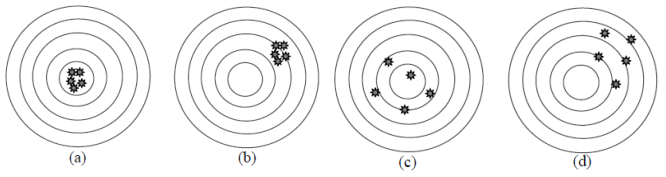
\includegraphics[width=0.75\linewidth]{./images/akurasi} 

}

\caption{4 ilustrasi terkait akurasi dan presisi}\label{fig:akurasi}
\end{figure}

Pada Gambar \ref{fig:akurasi} terdapat 4 buah kondisi ketika kita menembakkan beberapa perluru pada sebuah sasaran. Tujuan kita disini adalah untuk menembak bagian tengah sasaran tersebut.

Pada Gambar (a) dan (c) pada Gambar \ref{fig:akurasi} merupakan gambar yang menunjukkan seseorang telah berhasil mengenai bagian tengah sasaran tersebut dapat kita katakan pula tembakan pada kedua gambar tersebut akurat. Akurat dalam hal ini dapat diartikan suatu kondisi dimana kedekatan lubang peluru dengan pusat sasaran. Secara umum akurasi diartikan sebagai tingkat kedekatan pengukuran kuantitas terhadap nilai sebenarnya.

Terdapat dua buah cara untuk mengukur akurasi. Metode pengukuran akurasi antara lain: error absolut dan error relatif.

Error absolut merupakan nilai absolut dari selisih antara nilai sebenarnya \(x\) dengan nilai observasi \(x'\). Error absolut dapat dituliskan menggunakan Persamaan \eqref{eq:errorabsolut}.

\begin{equation}
   \epsilon_A=\left|x-x'\right|
  \label{eq:errorabsolut}
\end{equation}

Pengukuran lain yang sering digunakan untuk mengukur akurasi adalah error relatif. Berbeda dengan error absolut, error relatif membagi selisih antara nilai sebenarnya \(x\) dan nilai observasi \(x'\) dengan nilai sebenarnya. Hasil yang diperoleh merupakan nilai tanpa satuan. Persamaan error relatif disajikan pada Persamaan \eqref{eq:errorrelatif}.

\begin{equation}
   \epsilon_R=\left|\frac{x-x'}{x}\right|
  \label{eq:errorrelatif}
\end{equation}

Dalam suatu pengukuran, hal lain yang perlu diperhatikan selain akurasi adalah presisi. Presisi adalah sejauh mana pengulangan pengukuran dalam kondisi yang tidak berubah mendapat hasil yang sama. Berdasarkan Gambar \ref{fig:akurasi}, Gambar (a) dan (b) menunjukkan kepresisian yang tinggi. Hal ini terlihat dari jarak antara lubang peluru yang saling berdekatan dan mengelompok.

Berdasarkan Gambar \ref{fig:akurasi} dapat kita simpulkan bahwa dalam suatu sistem pengukuran akan terdapat 4 buah kondisi. Pengukuran akurat dan presisi (Gambar (a)), tidak akurat namun presisi (Gambar (b)), akurat namun tidak presisi (Gambar (c)), dan tidak akurat serta tidak presisi (Gambar (d)).

Dari kondisi-kondisi tersebut, akan meuncul yang dinamakan error. Dalam analisa numerik error atau kesalahan menjadi hal yang perlu diperhatikan.

\hypertarget{numerror}{%
\section{Error Numerik}\label{numerror}}

Kesalahan numerik merupakan error atau kesalahan yang timbul akibat adanya proses pendekatan atau hampiran. Kesalahan numerik terjadi karena tiga hal, antara lain:

\begin{itemize}
\item
  \textbf{Kesalahan bawaan (\emph{inherent error})}, merupakan kesalahan data yang timbul akibat adanya pengkuran, \emph{human error} seperti kesalahan pencatatan, atau tidak memahami hukum-hukum fisik dari data yang diukur.
\item
  \textbf{Kesalahan pembulatan (\emph{round-off error})}, adalah kesalahan yang terjadi karena adanya pembulatan. Contoh: 3,142857143\ldots{} menjadi 3,14.
\item
  \textbf{Kesalahan pemotongan (\emph{truncation error})}, adalah kesalahan yang ditimbulkan pada saat dilakukan pengurangan jumlah angka signifikan.
\end{itemize}

Kesalahan atau error dapat diukur menggunakan Persamaan \eqref{eq:errorabsolut} dan Persamaan \eqref{eq:errorrelatif} yang telah penulis jelaskan pada Chapter \ref{acuracy}.

\hypertarget{referensi-4}{%
\section{Referensi}\label{referensi-4}}

\begin{enumerate}
\def\labelenumi{\arabic{enumi}.}
\tightlist
\item
  Howard, J.P. 2017. \textbf{Computational Methods for Numerical Analysis with R}. CRC Press.
\item
  Sidiq, M. Tanpa Tahun. \textbf{Materi Kuliah Metode Numerik}. Repository Universitas Dian Nuswantoro.
\item
  Subakti, I. 2006. \textbf{Metode Numerik}. Institut Teknologi Sepuluh Nopember.
\item
  Sutarno,H., Rachmatin,D. 2008. \textbf{Hands Out Metode Numerik}. Universitas Pendidikan Indonesia.
\end{enumerate}

\hypertarget{linearaljabar}{%
\chapter{Aljabar Linier}\label{linearaljabar}}

Pada \emph{chapter} ini penulis akan menjelaskan mengenai cara untuk menyelesaikan sistem persamaan linier. Adapun yang akan dibahas pada \emph{chapter} ini antara lain:

\begin{itemize}
\tightlist
\item
  operasi Vektor dan matriks
\item
  Metode Eliminasi Gauss
\item
  Metode Dekomposisi matriks
\item
  Studi Kasus
\end{itemize}

\hypertarget{vecmat}{%
\section{Vektor dan matriks}\label{vecmat}}

Pada Chapter \ref{vector} dan Chapter \ref{matriks} telah dijelaskan sekilas bagaimana cara melakukan operasi pada vektor dan matriks. Pada \emph{chapter} ini, penulis akan menambahkan operasi-operasi lain yang dapat dilakukan pada vektor dan matriks. Dasar-dasar operasi ini selanjutnya akan digunakan sebagai dasar menyusun algoritma penyelesaian sistem persamaan linier.

\hypertarget{operasivektor}{%
\subsection{Operasi Vektor}\label{operasivektor}}

Misalkan saja diberikan vektor \(u\) dan \(v\) yang ditunjukkan pada Persamaan \eqref{eq:vectoruv}.

\begin{equation}
u = \begin{bmatrix}
      u_1            \\[0.3em]
      u_2            \\[0.3em]
      \vdots         \\[0.3em] 
      u_n
     \end{bmatrix}
dan\ v\ = \begin{bmatrix}
      v_1            \\[0.3em]
      v_2            \\[0.3em]
      \vdots         \\[0.3em] 
      v_n
     \end{bmatrix}
  \label{eq:vectoruv}
\end{equation}

Jika kita menambahkan atau mengurangkan nilai elemen vektor dengan suatu skalar (konstanta yang hanya memiliki besaran), maka operasi penjumlahan/pengurangan akan dilakukan pada setiap elemen vektor.

\begin{equation}
u \pm x = \begin{bmatrix}
      u_1            \\[0.3em]
      u_2            \\[0.3em]
      \vdots         \\[0.3em] 
      u_n
     \end{bmatrix}
\pm x = \begin{bmatrix}
      u_1 \pm x            \\[0.3em]
      u_2 \pm x           \\[0.3em]
      \vdots         \\[0.3em] 
      u_n \pm x
     \end{bmatrix}
     \label{eq:addvector}
\end{equation}

Jika kita melakukan penjumlahan pada vektor \(u\) dan \(v\), maka operasi akan terjadi pada masing-masing elemen dengan indeks yang sama.

\begin{equation}
u \pm v = \begin{bmatrix}
      u_1            \\[0.3em]
      u_2            \\[0.3em]
      \vdots         \\[0.3em] 
      u_n
     \end{bmatrix}
\pm v\ = \begin{bmatrix}
      v_1            \\[0.3em]
      v_2            \\[0.3em]
      \vdots         \\[0.3em] 
      v_n
     \end{bmatrix}
= \begin{bmatrix}
      u_1 \pm v_1            \\[0.3em]
      u_2 \pm v_2           \\[0.3em]
      \vdots         \\[0.3em] 
      u_n \pm v_n
     \end{bmatrix}
     \label{eq:addvector2}
\end{equation}

Untuk lebih memahami operasi tersebut, berikut penulis berikan contoh penerapannya pada \texttt{R}:

\begin{Shaded}
\begin{Highlighting}[]
\NormalTok{u }\OtherTok{\textless{}{-}} \FunctionTok{seq}\NormalTok{(}\DecValTok{1}\NormalTok{,}\DecValTok{5}\NormalTok{)}
\NormalTok{v }\OtherTok{\textless{}{-}} \FunctionTok{seq}\NormalTok{(}\DecValTok{6}\NormalTok{,}\DecValTok{10}\NormalTok{)}

\CommentTok{\# penjumlahan}
\NormalTok{u}\SpecialCharTok{+}\NormalTok{v}
\end{Highlighting}
\end{Shaded}

\begin{verbatim}
## [1]  7  9 11 13 15
\end{verbatim}

\begin{Shaded}
\begin{Highlighting}[]
\CommentTok{\# penguranga}
\NormalTok{u}\SpecialCharTok{{-}}\NormalTok{v}
\end{Highlighting}
\end{Shaded}

\begin{verbatim}
## [1] -5 -5 -5 -5 -5
\end{verbatim}

Bagaimana jika kita melakukan operasi dua vektor, dimaana salah satu vektor memiliki penjang yang berbeda?. Untuk memnjawab hal tersebut, perhatikan sintaks berikut:

\begin{Shaded}
\begin{Highlighting}[]
\NormalTok{x }\OtherTok{\textless{}{-}} \FunctionTok{seq}\NormalTok{(}\DecValTok{1}\NormalTok{,}\DecValTok{2}\NormalTok{)}
\NormalTok{u}\SpecialCharTok{+}\NormalTok{x}
\end{Highlighting}
\end{Shaded}

\begin{verbatim}
## Warning in u + x: longer object length is not a
## multiple of shorter object length
\end{verbatim}

\begin{verbatim}
## [1] 2 4 4 6 6
\end{verbatim}

Berdasarkan contoh tersebut, \texttt{R} akan mengeluarkan peringatan yang menunjukkan operasi dilakukan pada vektor dengan panjang berbeda. \texttt{R} akan tetap melakukan perhitungan dengan menjumlahkan kembali vektor \(u\) yang belum dijumlahkan dengan vektor \(x\) sampai seluruh elemen vektor \(u\) dilakukan operasi penjumlahan.

Operasi lain yang dapat dilakukan pada vektor adalah menghitung \emph{inner product} dan panjang vektor. Inner product dihitung menggunakan Persamaan \eqref{eq:innerproduct}.

\begin{equation}
u.v=\sum_{i=1}^nu_1v_1+u_2v_2+\dots+u_nv_n
  \label{eq:innerproduct}
\end{equation}

Panjang vektor atau vektor yang telah dinormalisasi dihitung menggunakan Persamaan \eqref{eq:panjangvektor}

\begin{equation}
\left|u\right|=\sqrt{u_1^2+u_2^2+\dots+u_n^2}
  \label{eq:panjangvektor}
\end{equation}

Berikut adalah contoh bagaimana cara menghitung \texttt{inner\ product} dan panjang vektor menggunakan \texttt{R}:

\begin{Shaded}
\begin{Highlighting}[]
\CommentTok{\# inner product}
\NormalTok{u}\SpecialCharTok{\%*\%}\NormalTok{v}
\end{Highlighting}
\end{Shaded}

\begin{verbatim}
##      [,1]
## [1,]  130
\end{verbatim}

\begin{Shaded}
\begin{Highlighting}[]
\CommentTok{\# panjang vektor u}
\FunctionTok{sqrt}\NormalTok{(}\FunctionTok{sum}\NormalTok{(u}\SpecialCharTok{*}\NormalTok{u))}
\end{Highlighting}
\end{Shaded}

\begin{verbatim}
## [1] 7.416
\end{verbatim}

\hypertarget{operasimatrik}{%
\subsection{Operasi matriks}\label{operasimatrik}}

Misalkan kita memiliki 2 buah matriks \(A\) dan \(B\).

\begin{equation}
A = \begin{bmatrix}
       a_{1.1} & a_{1.2} &\cdots& a_{1.n}           \\[0.3em]
       a_{2.1} & a_{2.2} &\cdots& a_{2.n}           \\[0.3em]
       \vdots  & \vdots  &\ddots& \vdots            \\[0.3em]
       a_{m.1} & a_{m.2} &\cdots& a_{m.n}
     \end{bmatrix}
dan\ B = \begin{bmatrix}
      b_{1.1} & b_{1.2} &\cdots& b_{1.n}           \\[0.3em]
      b_{2.1} & b_{2.2} &\cdots& b_{2.n}           \\[0.3em]
      \vdots  & \vdots  &\ddots& \vdots            \\[0.3em]
      b_{m.1} & b_{m.2} &\cdots& b_{m.n}
     \end{bmatrix}
  \label{eq:matrikuv}
\end{equation}

Jika salah satu matriks tersebut dijumlahkan atau dikurangkan dengan skalar.

\begin{equation}
A \pm x = \begin{bmatrix}
       a_{1.1} & a_{1.2} &\cdots& a_{1.n}           \\[0.3em]
       a_{2.1} & a_{2.2} &\cdots& a_{2.n}           \\[0.3em]
       \vdots  & \vdots  &\ddots& \vdots            \\[0.3em]
       a_{m.1} & a_{m.2} &\cdots& a_{m.n}
     \end{bmatrix}
\pm x = \begin{bmatrix}
      a_{1.1}\pm x & a_{1.2}\pm x &\cdots& a_{1.n}\pm x           \\[0.3em]
      a_{2.1}\pm x & a_{2.2}\pm x &\cdots& a_{2.n}\pm x           \\[0.3em]
      \vdots  & \vdots  &\ddots& \vdots            \\[0.3em]
      a_{m.1}\pm x & a_{m.2}\pm x &\cdots& a_{m.n}\pm x
     \end{bmatrix}
  \label{eq:addmatrik}
\end{equation}

Jika kedua matriks \(A\) dan \(B\) saling dijumlahkan atau dikurangkan. Perlu diperhatikan bahwa penjumlahan dua buah matriks hanya dapat dilakukan pada matriks dengan ukuran yang seragam.

\begin{equation}
\begin{split}
A \pm B & = \begin{bmatrix}
       a_{1.1} & a_{1.2} &\cdots& a_{1.n}           \\[0.3em]
       a_{2.1} & a_{2.2} &\cdots& a_{2.n}           \\[0.3em]
       \vdots  & \vdots  &\ddots& \vdots            \\[0.3em]
       a_{m.1} & a_{m.2} &\cdots& a_{m.n}
     \end{bmatrix}
\pm \begin{bmatrix}
      b_{1.1} & b_{1.2} &\cdots& b_{1.n}           \\[0.3em]
      b_{2.1} & b_{2.2} &\cdots& b_{2.n}           \\[0.3em]
      \vdots  & \vdots  &\ddots& \vdots            \\[0.3em]
      b_{m.1} & b_{m.2} &\cdots& b_{m.n}
     \end{bmatrix} \\
& = \begin{bmatrix}
       a_{1.1}\pm b_{1.1} & a_{1.2}\pm b_{1.2} &\cdots& a_{1.n}\pm b_{1.n}           \\[0.3em]
       a_{2.1}\pm b_{2.1} & a_{2.2}\pm b_{2.2} &\cdots& a_{2.n}\pm b_{2.n}           \\[0.3em]
       \vdots  & \vdots  &\ddots& \vdots            \\[0.3em]
       a_{m.1}\pm b_{m.1} & a_{m.2}\pm b_{m.2} &\cdots& a_{m.n}\pm b_{m.n}
     \end{bmatrix}
\end{split}
  \label{eq:addmatrik2}
\end{equation}

Untuk lebih memahaminya, berikut disajikan contoh operasi penjumlahan pada matriks:

\begin{Shaded}
\begin{Highlighting}[]
\NormalTok{A }\OtherTok{\textless{}{-}} \FunctionTok{matrix}\NormalTok{(}\DecValTok{1}\SpecialCharTok{:}\DecValTok{9}\NormalTok{,}\DecValTok{3}\NormalTok{)}
\NormalTok{B }\OtherTok{\textless{}{-}} \FunctionTok{matrix}\NormalTok{(}\DecValTok{10}\SpecialCharTok{:}\DecValTok{18}\NormalTok{,}\DecValTok{3}\NormalTok{)}
\NormalTok{C }\OtherTok{\textless{}{-}} \FunctionTok{matrix}\NormalTok{(}\DecValTok{1}\SpecialCharTok{:}\DecValTok{6}\NormalTok{,}\DecValTok{3}\NormalTok{)}

\CommentTok{\# penjumlahan dengan skalar}
\NormalTok{A}\SpecialCharTok{+}\DecValTok{1}
\end{Highlighting}
\end{Shaded}

\begin{verbatim}
##      [,1] [,2] [,3]
## [1,]    2    5    8
## [2,]    3    6    9
## [3,]    4    7   10
\end{verbatim}

\begin{Shaded}
\begin{Highlighting}[]
\CommentTok{\# penjumlahan A+B}
\NormalTok{A}\SpecialCharTok{+}\NormalTok{B}
\end{Highlighting}
\end{Shaded}

\begin{verbatim}
##      [,1] [,2] [,3]
## [1,]   11   17   23
## [2,]   13   19   25
## [3,]   15   21   27
\end{verbatim}

\begin{Shaded}
\begin{Highlighting}[]
\CommentTok{\# penjumlahan}
\NormalTok{A}\SpecialCharTok{+}\NormalTok{C}
\end{Highlighting}
\end{Shaded}

Operasi pehitungan lain yang penting pada matriks adalah operasi perkalian matriks. Perlu diperhatikan bahwa untuk perkalian matriks, jumlah kolom matriks sebelah kiri harus sama dengan jumlah baris pada matriks sebelah kanan. Perkalian antara dua matriks disajikan pada Persamaan \eqref{eq:kalimatrik}.

\begin{equation}
A_{m.n}\times B_{n.r}=AB_{m.r}
  \label{eq:kalimatrik}
\end{equation}

Pada \texttt{R} perkalian matriks dilakukan menggunakan operator \texttt{\%*\%}. Berikut adalah contoh perkalian matriks pada \texttt{R}:

\begin{Shaded}
\begin{Highlighting}[]
\CommentTok{\# Perkalian matriks}
\NormalTok{A}\SpecialCharTok{\%*\%}\NormalTok{B}
\end{Highlighting}
\end{Shaded}

\begin{verbatim}
##      [,1] [,2] [,3]
## [1,]  138  174  210
## [2,]  171  216  261
## [3,]  204  258  312
\end{verbatim}

\hypertarget{rowoperation}{%
\section{Operasi Baris Elementer}\label{rowoperation}}

Terdapat tiga buah operasi dasar pada baris matriksoperasi baris elementer. Ketiga operasi ini akan menjadi dasar operasi \emph{sub-chapter} selanjutnya. Ketiga operasi dasar tersebut antara lain:

\begin{enumerate}
\def\labelenumi{\arabic{enumi}.}
\tightlist
\item
  \textbf{\emph{Row Scalling}}. Mengalikan baris matriks dengan konstanta bukan nol.
\item
  \textbf{\emph{Row Swaping}}. Menukar urutan baris pada sebuah matriks (contoh: menukar baris 1 dengan baris 2 dan sebaliknya).
\item
  \textbf{\emph{Row Replacement}}. Baris matriks diganti dengan hasil penjumlahan atau pengurangan baris matriks tersebut dengan baris matriks lainnya, dimana baris matriks lainnya yang akan dijumlahkan/dikurangkan dengan matriks tersebut telah dilakukan proses \emph{row scalling}. Luaran yang diperoleh pada umumnya adalah nilai nol pada baris matriks awal atau akhir.
\end{enumerate}

Ketiga proses tersebut akan terjadi secara berulang, khusunya jika kita hendak mengerjakan sistem persamaan linier menggunakan algoritma eliminasi Gauss. Untuk mempermudah proses tersebut, kita dapat membuat masing-masing fungsi untuk masing-masing operasi tersebut. Algoritma fungsi-fungsi tersebut selanjutnya menjadi dasar penyusunan algoritma fungsi-fungsi eliminasi Gauss dan dekomposisi matriks yang akan dijelaskan pada \emph{chapter} selanjutnya.

Fungsi \emph{row scalling} pada \texttt{R} dapat dituliskan pada sintaks berikut:

\begin{Shaded}
\begin{Highlighting}[]
\NormalTok{scale\_row }\OtherTok{\textless{}{-}} \ControlFlowTok{function}\NormalTok{(m, row, k)\{}
\NormalTok{ m[row, ] }\OtherTok{\textless{}{-}}\NormalTok{ m[row, ]}\SpecialCharTok{*}\NormalTok{k}
 \FunctionTok{return}\NormalTok{(m)}
\NormalTok{\}}
\end{Highlighting}
\end{Shaded}

Berikut adalah contoh penerapannya:

\begin{Shaded}
\begin{Highlighting}[]
\CommentTok{\# membuat matriks A}
\NormalTok{(A }\OtherTok{\textless{}{-}} \FunctionTok{matrix}\NormalTok{(}\DecValTok{1}\SpecialCharTok{:}\DecValTok{15}\NormalTok{, }\AttributeTok{nrow=}\DecValTok{5}\NormalTok{))}
\end{Highlighting}
\end{Shaded}

\begin{verbatim}
##      [,1] [,2] [,3]
## [1,]    1    6   11
## [2,]    2    7   12
## [3,]    3    8   13
## [4,]    4    9   14
## [5,]    5   10   15
\end{verbatim}

\begin{Shaded}
\begin{Highlighting}[]
\CommentTok{\# lakukan scaling pada row 2 dengan nilai 10}
\FunctionTok{scale\_row}\NormalTok{(}\AttributeTok{m=}\NormalTok{A, }\AttributeTok{row=}\DecValTok{2}\NormalTok{, }\DecValTok{10}\NormalTok{)}
\end{Highlighting}
\end{Shaded}

\begin{verbatim}
##      [,1] [,2] [,3]
## [1,]    1    6   11
## [2,]   20   70  120
## [3,]    3    8   13
## [4,]    4    9   14
## [5,]    5   10   15
\end{verbatim}

\begin{quote}
\textbf{Catatan:} Untuk menyimpan hasil perhitungan, simpan proses perhitungan dalam sebuah objek (lihat Chapter \ref{assigningvar}).
\end{quote}

\emph{Row swapping} merupakan proses yang berulang, kita perlu menyimpan terlebih dahulu baris matriks pertama kedalam sebuah objek. Baris matriks pertama selanjutnya diganti dengan baris matriks kedua, sedangkan baris matriks kedua selanjutnya akan diganti dengan baris matriks pertama yang telah terlebih dahulu disimpan dalam sebuah objek. Fungsi \emph{row swapping} pada \texttt{R} dapat dituliskan pada sintaks berikut:

\begin{Shaded}
\begin{Highlighting}[]
\NormalTok{swap\_row }\OtherTok{\textless{}{-}} \ControlFlowTok{function}\NormalTok{(m, row1, row2)\{}
\NormalTok{  row\_tmp }\OtherTok{\textless{}{-}}\NormalTok{ m[row1, ]}
\NormalTok{  m[row1, ] }\OtherTok{\textless{}{-}}\NormalTok{ m[row2, ]}
\NormalTok{  m[row2, ] }\OtherTok{\textless{}{-}}\NormalTok{ row\_tmp}
  \FunctionTok{return}\NormalTok{(m)}
\NormalTok{\}}
\end{Highlighting}
\end{Shaded}

Berikut merupakan contoh penerapan fungsi \texttt{swap\_row()}:

\begin{Shaded}
\begin{Highlighting}[]
\CommentTok{\# pertukarkan baris 2 dengan baris 5}
\FunctionTok{swap\_row}\NormalTok{(}\AttributeTok{m=}\NormalTok{A, }\AttributeTok{row1=}\DecValTok{2}\NormalTok{, }\AttributeTok{row2=}\DecValTok{5}\NormalTok{)}
\end{Highlighting}
\end{Shaded}

\begin{verbatim}
##      [,1] [,2] [,3]
## [1,]    1    6   11
## [2,]    5   10   15
## [3,]    3    8   13
## [4,]    4    9   14
## [5,]    2    7   12
\end{verbatim}

Pada proses \emph{row replacement}, proses perhitungan dilakukan dengan melakukan penjumlahan suatu baris matriks dengan baris matriks lainnya dengan terlebih dahulu melakukan \emph{row scalling} terhadap matriks lainnya. Berikut adalah fungsi \texttt{replace\_row()} yang ditulis pada \texttt{R}:

\begin{Shaded}
\begin{Highlighting}[]
\NormalTok{replace\_row }\OtherTok{\textless{}{-}} \ControlFlowTok{function}\NormalTok{(m, row1, row2, k)\{}
\NormalTok{  m[row2, ] }\OtherTok{\textless{}{-}}\NormalTok{ m[row2, ] }\SpecialCharTok{+}\NormalTok{ m[row1, ]}\SpecialCharTok{*}\NormalTok{k}
  \FunctionTok{return}\NormalTok{(m)}
\NormalTok{\}}
\end{Highlighting}
\end{Shaded}

Berikut adalah contoh penerapan fungsi \texttt{replace\_row()}:

\begin{Shaded}
\begin{Highlighting}[]
\FunctionTok{replace\_row}\NormalTok{(}\AttributeTok{m=}\NormalTok{A, }\AttributeTok{row1=}\DecValTok{1}\NormalTok{, }\AttributeTok{row2=}\DecValTok{3}\NormalTok{, }\AttributeTok{k=}\SpecialCharTok{{-}}\DecValTok{3}\NormalTok{)}
\end{Highlighting}
\end{Shaded}

\begin{verbatim}
##      [,1] [,2] [,3]
## [1,]    1    6   11
## [2,]    2    7   12
## [3,]    0  -10  -20
## [4,]    4    9   14
## [5,]    5   10   15
\end{verbatim}

\hypertarget{gausselimination}{%
\section{Eliminasi Gauss}\label{gausselimination}}

Pada \emph{sub-chapter} ini kita akan menggunakan operasi baris elementer yang telah dijelaskan pada Chapter \ref{assigningvar}. Terdapat dua topik yang akan dibahas pada \emph{sub-chapter} ini, yaitu: \emph{row echelon form} termasuk \emph{reduced row echelon form} dan matriks tridiagonal.

Eliminasi Gauss merupakan sebuah cara untuk mencari penyelesaian sistem persamaan linier. Ide dasar dari eliminasi Gauss adalah melakukan operasi matematika pada baris matriks (lihat Chapter \ref{assigningvar}) dan melanjutkannya sampai hanya tersisa satu variabel saja. Kita dapat melakukan lebih dari satu operasi baris elementer pada proses elmininasi ini (contoh: mengalikan sebuah baris dengan konstanta dan menjumlahkan hasilnya pada baris lain).

\hypertarget{rowechelonform}{%
\subsection{\texorpdfstring{\emph{Row Echelon Form}}{Row Echelon Form}}\label{rowechelonform}}

Sebuah matriks merupakan \emph{row echelon form} jika matriks tersebut memenuhi beberapa kondisi:

\begin{enumerate}
\def\labelenumi{\arabic{enumi}.}
\tightlist
\item
  Angka bukan nol pertama dari kiri (\emph{leading coefficient}) selalu di sebelah kanan angka bukan nol pertama pada baris di atasnya.
\item
  Baris yang terdiri dari semua nol ada di bagian bawah matriks.
\end{enumerate}

Misalkan terdapat persamaan linier seperti yang ditunjukkan pada Persamaan \eqref{eq:spl}.

\begin{equation}
\begin{matrix}
  a_{1.1}x_1+a_{1.2}x_2+a_{1.3}x_3+\cdots+a_{1.n}x_n=b_1 \\
  a_{2.1}x_1+a_{2.2}x_2+a_{2.3}x_3+\cdots+a_{2.n}x_n=b_2 \\
  a_{3.1}x_1+a_{3.2}x_2+a_{3.3}x_3+\cdots+a_{3.n}x_n=b_3 \\
  \cdots\cdots\cdots\cdots\cdots\cdots\cdots\cdots       \\
  a_{m.1}x_1+a_{m.2}x_2+a_{m.3}x_3+\cdots+a_{m.n}x_n=b_n
 \end{matrix}
  \label{eq:spl}
\end{equation}

dimana \(a_{i.j}\) untuk \(i=1\) sampai dengan \(m\) dan \(j=1\) sampai dengan \(n\) merupakan koefisien persamaan linier. \(x_i\) untuk \(i=1\) sampai dengan \(n\) merupakan variabel bebas pada sistem persamaan linier.

Persamaan linier pada Persamaan \eqref{eq:spl} dapat dinyatakan ke dalam bentuk matriks pada Persamaan \eqref{eq:matrikpl}.

\begin{equation}
\begin{bmatrix}
     a_{1.1} & a_{1.2} & a_{1.3} &\cdots& a_{1.n}           \\[0.3em]
     a_{2.1} & a_{2.2} & a_{2.3} &\cdots& a_{2.n}           \\[0.3em]
     a_{3.1} & a_{3.2} & a_{3.3} &\cdots& a_{3.n}           \\[0.3em]
     \vdots  & \vdots  & \vdots  &\ddots& \vdots            \\[0.3em]
     a_{m.1} & a_{m.2} & a_{m.3} &\cdots& a_{m.n}
     \end{bmatrix}
\begin{bmatrix}
     x_1                                          \\[0.3em]
     x_2                                          \\[0.3em]
     x_3                                          \\[0.3em]
     \cdots                                       \\[0.3em]
     x_n                                       
     \end{bmatrix}
= \begin{bmatrix}
     b_1                                          \\[0.3em]
     b_2                                          \\[0.3em]
     b_3                                          \\[0.3em]
     \cdots                                       \\[0.3em]
     b_n                                       
     \end{bmatrix}
  \label{eq:matrikpl}
\end{equation}

\begin{equation}
AX=B
  \label{eq:matrikpl2}
\end{equation}

dimana:

\begin{itemize}
\tightlist
\item
  matriks A merupakan matriks koefisien / Jacobian
\item
  vaktor X merupakan vaktor variabel
\item
  vektor B merupakan vektor konstanta
\end{itemize}

matriks pada Persamaan \eqref{eq:matrikpl} dapat diubah menjadi \emph{augmented matrix}, yaitu: perluasan matriks A dengan menambahkan vektor B pada kolom terakhirnya.

\begin{equation}
\begin{bmatrix}
     a_{1.1} & a_{1.2} & a_{1.3} &\cdots& a_{1.n} & b_1     \\[0.3em]
     a_{2.1} & a_{2.2} & a_{2.3} &\cdots& a_{2.n} & b_2     \\[0.3em]
     a_{3.1} & a_{3.2} & a_{3.3} &\cdots& a_{3.n} & b_3     \\[0.3em]
     \vdots  & \vdots  & \vdots &\ddots& \vdots            \\[0.3em]
     a_{m.1} & a_{m.2} & a_{m.3} &\cdots& a_{m.n} & b_n
     \end{bmatrix}
  \label{eq:augmatrik}
\end{equation}

\begin{equation}
A=\left[A|B\right]
  \label{eq:augmatrik2}
\end{equation}

\begin{theorem}[spltheorem]
\protect\hypertarget{thm:unnamed-chunk-134}{}\label{thm:unnamed-chunk-134}Suatu sistem persamaan linier mempunyai penyelesaian tunggal bila memenuhi syarat-syarat sebagai berikut:
\end{theorem}

\begin{itemize}
\tightlist
\item
  ukuran persamaan linier simultan bujursangkar (jumlah persamaan sama dengan jumlah variabel bebas).
\item
  sistem persamaan linier \emph{non-homogen} di mana minimal ada satu nilai vektor konstanta \(B\) tidak nol atau terdapat \(b_{n}\neq 0\).
\item
  Determinan dari matriks koefisiensistem persamaan linier tidak sama dengan nol.
\end{itemize}

Untuk memperoleh penyelesaian sistem persamaan linier, Persamaan \eqref{eq:augmatrik} perlu dilakukan operasi baris elementer. Hasil operasi baris dasar akan menghasilkan matriks \emph{row echelon form} yang disajikan pada Persamaan \eqref{eq:refeq}.

\begin{equation}
\begin{bmatrix}
     a_{1.1} & a_{1.2} & a_{1.3} &\cdots& a_{1.n} & b_1     \\[0.3em]
     a_{2.1} & a_{2.2} & a_{2.3} &\cdots& a_{2.n} & b_2     \\[0.3em]
     a_{3.1} & a_{3.2} & a_{3.3} &\cdots& a_{3.n} & b_3     \\[0.3em]
     \vdots  & \vdots  & \vdots &\ddots& \vdots             \\[0.3em]
     a_{m.1} & a_{m.2} & a_{m.3} &\cdots& a_{m.n} & b_n
     \end{bmatrix}
\implies
\begin{bmatrix}
     c_{1.1} & c_{1.2} & c_{1.3} &\cdots& c_{1.n} & d_1     \\[0.3em]
     0       & c_{2.2} & c_{2.3} &\cdots& c_{2.n} & d_2     \\[0.3em]
     0       & 0       & c_{3.3} &\cdots& c_{3.n} & d_3     \\[0.3em]
     \vdots  & \vdots  & \vdots &\ddots& \vdots             \\[0.3em]
     0       & 0       & 0      &\cdots& c_{m.n} & d_n
     \end{bmatrix}
  \label{eq:refeq}
\end{equation}

Sehingga penyelesaian sistem persamaan linier dapat diperoleh menggunakan Persamaan \eqref{eq:refsolution}.

\begin{equation}
\begin{matrix}
  x_n=\frac{d_n}{c_{m.n}} \\
  x_{n-1}=\frac{1}{C_{m-1.n-1}}\left(d_{n-1}-c_{m-1.n}x_n\right) \\
  \cdots\cdots\cdots\cdots\cdots\cdots\cdots\cdots       \\
  x_2=\frac{1}{c_{2.2}}\left(d_2-c_{2.3}x_3-c_{2.4}x_4-\dots-c_{2.n}x_n\right) \\
  x_1=\frac{1}{c_{1.1}}\left(d_1-c_{1.2}x_2-c_{1.3}x_3-\dots-c_{1.n}x_n\right)
   \end{matrix}
  \label{eq:refsolution}
\end{equation}

\begin{example}
\protect\hypertarget{exm:refexm}{}\label{exm:refexm}Selesaikan sistem persamaan berikut:
\end{example}

\[
\begin{matrix}
  x_1+x_2+x_3=6 \\
  x_1+2x_2-x_3=2 \\
  2x_1+x_2+2x_3=10 \\
\end{matrix}
\]

\textbf{Jawab}:

\emph{Augmented matrix} sistem persamaan linier tersebut adalah sebagai berikut:

\[
\begin{bmatrix}
     1 & 1 & 1 & 6     \\[0.3em]
     1 & 2 & -1 & 2     \\[0.3em]
     2 & 1 & 2 & 10
\end{bmatrix}
\]

Operasi baris elementer selanjutnya dilakukan pada matriks tersebut. Pada langkah pertama, baris ke-2 dikurangkan dengan baris ke-1 (\(B_2-B_1\)) dan baris ke-3 dikurangkan oleh dua kali baris ke-1 (\(B_3-2B_1\)).

\begin{equation*}
\begin{bmatrix}
     1 & 1 & 1 & 6     \\[0.3em]
     1 & 2 & -1 & 2     \\[0.3em]
     2 & 1 & 2 & 10
\end{bmatrix}
\begin{matrix}
  B_2-B_1 \\
  \implies \\
  B_3-2B_1
\end{matrix}
\begin{bmatrix}
     1 & 1 & 1 & 6     \\[0.3em]
     0 & 1 & -2 & -4     \\[0.3em]
     0 & -1 & 0 & -2
\end{bmatrix}
\end{equation*}

Hasil dari langkah pertama tersebut, selanjutnya menjadi input dari langkah selanjutnya. Pada langkah selanjutnya operasi baris elementer kembali dilanjutkan. Baris ke-3 dikurangkan denganbaris ke-2 (\(B_3-B_2\)).

\begin{equation*}
\begin{bmatrix}
     1 & 1 & 1 & 6     \\[0.3em]
     0 & 1 & -2 & -4     \\[0.3em]
     0 & -1 & 0 & -2
\end{bmatrix}
\begin{matrix}
  B_3-B_2 \\
  \implies
\end{matrix}
\begin{bmatrix}
     1 & 1 & 1 & 6     \\[0.3em]
     0 & 1 & -2 & -4     \\[0.3em]
     0 & 0 & -2 & -6
\end{bmatrix}
\end{equation*}

Setelah diperoleh matriks \emph{row echelon form} selanjutnya penyelesaian persamaan dapat dikerjakan menggunakan Persamaan \eqref{eq:refsolution}.

\begin{equation*}
\begin{matrix}
  x_3=\frac{-6}{-2}=3 \\
  x_2=\frac{1}{1}\left(-4-\left(2\right)3\right)=2 \\
  x_1=\frac{1}{1}\left(6-2-3\right)=1
\end{matrix}
\end{equation*}

\begin{center}\rule{0.5\linewidth}{0.5pt}\end{center}

\textbf{Algoritma Row Echelon Form}

\begin{enumerate}
\def\labelenumi{\arabic{enumi}.}
\tightlist
\item
  Masukkan matriks \(A\), dan vektor \(B\) beserta ukurannya \(n\)
\item
  Buat \emph{augmented matrix} \(\left[A|B\right]\) namakan dengan \(A\)
\item
  Untuk baris ke-\(i\) dimana \(i=1\) s/d \(n\), perhatikan apakah nilai \(a_{i,j}\) sama dengan nol. \textbf{a)} \textbf{Bila iya}, lakukan \emph{row swapping} antara baris ke-\(i\) dan baris ke-\(i+k\leq n\), dimana \(a_{i+k,j}\) tidak sama dengan nol. Bila tidak ada berarti perhitungan tidak bisa dilanjutkan dan proses dihentikan dengan tanpa penyelesaian, \textbf{b)} \textbf{Bila tidak}, lanjutkan.
\item
  Untuk baris ke-\(j\), dimana \(j=i+1\) s/d \(n\), lakukan operasi baris elementer:\textbf{a)} Hitung \(c=\frac{a_{j,i}}{a_{i,i}}\), \textbf{b)} untuk kolom \(k\), dimana \(k=1\) s/d \(n+1\), hitung \(a_{j,k}=a_{j,k}-c.a_{i,k}\).
\item
  Hitung akar, untuk \(i=n\) s/d 1 (bergerak dari baris pertama) menggunakan Persamaan \eqref{eq:refsolution}.
\end{enumerate}

\begin{center}\rule{0.5\linewidth}{0.5pt}\end{center}

Berdasarkan algoritma tersebut, kita dapat menyusun fungsi pada \texttt{R} untuk menyelesaikan sistem persamaan linier menggunakan matriks \emph{row echelon form}. Fungsi yang akan dibentuk hanya sampai pada algoritma ke-4. Proses substitusi akan dilakukan secara manual. Berikut adalah sintaks yang digunakan:

\begin{Shaded}
\begin{Highlighting}[]
\NormalTok{ref\_matrix }\OtherTok{\textless{}{-}} \ControlFlowTok{function}\NormalTok{(a)\{}
\NormalTok{  m }\OtherTok{\textless{}{-}} \FunctionTok{nrow}\NormalTok{(a)}
\NormalTok{  n }\OtherTok{\textless{}{-}} \FunctionTok{ncol}\NormalTok{(a)}
\NormalTok{  piv }\OtherTok{\textless{}{-}} \DecValTok{1}
  
\CommentTok{\# cek elemen diagonal apakah bernilai nol}
  \ControlFlowTok{for}\NormalTok{(row\_curr }\ControlFlowTok{in} \DecValTok{1}\SpecialCharTok{:}\NormalTok{m)\{}
    \ControlFlowTok{if}\NormalTok{(piv }\SpecialCharTok{\textless{}=}\NormalTok{ n)\{}
\NormalTok{      i }\OtherTok{\textless{}{-}}\NormalTok{ row\_curr}
      \ControlFlowTok{while}\NormalTok{(a[i, piv] }\SpecialCharTok{==} \DecValTok{0} \SpecialCharTok{\&\&}\NormalTok{ i }\SpecialCharTok{\textless{}}\NormalTok{ m)\{}
\NormalTok{        i }\OtherTok{\textless{}{-}}\NormalTok{ i}\SpecialCharTok{+}\DecValTok{1}
        \ControlFlowTok{if}\NormalTok{(i }\SpecialCharTok{\textgreater{}}\NormalTok{ m)\{}
\NormalTok{          i }\OtherTok{\textless{}{-}}\NormalTok{ row\_curr}
\NormalTok{          piv }\OtherTok{\textless{}{-}}\NormalTok{ piv}\SpecialCharTok{+}\DecValTok{1}
          \ControlFlowTok{if}\NormalTok{(piv }\SpecialCharTok{\textgreater{}}\NormalTok{ n)}
            \FunctionTok{return}\NormalTok{(a)}
\NormalTok{        \}}
\NormalTok{      \}}
      
\CommentTok{\# jika diagonal bernilai nol, lakukan row swapping}
    \ControlFlowTok{if}\NormalTok{(i }\SpecialCharTok{!=}\NormalTok{ row\_curr)}
\NormalTok{      a }\OtherTok{\textless{}{-}} \FunctionTok{swap\_row}\NormalTok{(a, i, row\_curr)}
    
\CommentTok{\# proses triangulasi untuk membentuk matriks segitiga atas}
    \ControlFlowTok{for}\NormalTok{(j }\ControlFlowTok{in}\NormalTok{ row\_curr}\SpecialCharTok{:}\NormalTok{m)}
      \ControlFlowTok{if}\NormalTok{(j }\SpecialCharTok{!=}\NormalTok{ row\_curr)\{}
\NormalTok{        c }\OtherTok{\textless{}{-}}\NormalTok{ a[j, piv]}\SpecialCharTok{/}\NormalTok{a[row\_curr, piv]}
\NormalTok{        a }\OtherTok{\textless{}{-}} \FunctionTok{replace\_row}\NormalTok{(a, row\_curr, j, }\SpecialCharTok{{-}}\NormalTok{c)}
\NormalTok{      \}}
\NormalTok{    piv }\OtherTok{\textless{}{-}}\NormalTok{ piv}\SpecialCharTok{+}\DecValTok{1}
\NormalTok{    \}}
\NormalTok{  \}}
  \FunctionTok{return}\NormalTok{(a)}
\NormalTok{\}}
\end{Highlighting}
\end{Shaded}

Dengan menggunakan fungsi \texttt{ref\_matrix()}, kita dapat membentuk matriks \emph{row echelon form} pada Contoh \ref{exm:refexm}.

\begin{Shaded}
\begin{Highlighting}[]
\NormalTok{am }\OtherTok{\textless{}{-}} \FunctionTok{c}\NormalTok{(}\DecValTok{1}\NormalTok{,}\DecValTok{1}\NormalTok{,}\DecValTok{2}\NormalTok{,}
        \DecValTok{1}\NormalTok{,}\DecValTok{2}\NormalTok{,}\DecValTok{1}\NormalTok{,}
        \DecValTok{1}\NormalTok{,}\SpecialCharTok{{-}}\DecValTok{1}\NormalTok{,}\DecValTok{2}\NormalTok{,}
        \DecValTok{6}\NormalTok{,}\DecValTok{2}\NormalTok{,}\DecValTok{10}\NormalTok{)}
\NormalTok{(m }\OtherTok{\textless{}{-}} \FunctionTok{matrix}\NormalTok{(am, }\AttributeTok{nrow=}\DecValTok{3}\NormalTok{))}
\end{Highlighting}
\end{Shaded}

\begin{verbatim}
##      [,1] [,2] [,3] [,4]
## [1,]    1    1    1    6
## [2,]    1    2   -1    2
## [3,]    2    1    2   10
\end{verbatim}

\begin{Shaded}
\begin{Highlighting}[]
\FunctionTok{ref\_matrix}\NormalTok{(m)}
\end{Highlighting}
\end{Shaded}

\begin{verbatim}
##      [,1] [,2] [,3] [,4]
## [1,]    1    1    1    6
## [2,]    0    1   -2   -4
## [3,]    0    0   -2   -6
\end{verbatim}

matriks yang diperoleh selanjutnya dapat diselesaikan menggunakan Persamaan \eqref{eq:refsolution}.

\begin{example}
\protect\hypertarget{exm:refexm2}{}\label{exm:refexm2}Dengan menggunakan fungsi \texttt{ref\_matrix()}, buatlah matriks \emph{row echelon form} dari sistem persamaan linier berikut:
\end{example}

\[
\begin{matrix}
  2x_1+x_2-x_3=1 \\
  3x_1+2x_2-2x_3=1 \\
  x_1-5x_2+4x_3=3 \\
\end{matrix}
\]

\textbf{Jawab}:

\emph{Augmented matrix} dari sistem persamaan tersebut adalah sebagai berikut:

\[
\begin{bmatrix}
     2 & 1 & -1 & 1     \\[0.3em]
     3 & 2 & -2 & 1     \\[0.3em]
     1 & -5 & 4 & 3
\end{bmatrix}
\]

Penyelesaian matriks tersebut adalah sebagai berikut:

\begin{Shaded}
\begin{Highlighting}[]
\NormalTok{(m }\OtherTok{\textless{}{-}} \FunctionTok{matrix}\NormalTok{(}\FunctionTok{c}\NormalTok{(}\DecValTok{2}\NormalTok{,}\DecValTok{3}\NormalTok{,}\DecValTok{1}\NormalTok{,}
              \DecValTok{1}\NormalTok{,}\DecValTok{2}\NormalTok{,}\SpecialCharTok{{-}}\DecValTok{5}\NormalTok{,}
              \SpecialCharTok{{-}}\DecValTok{1}\NormalTok{,}\SpecialCharTok{{-}}\DecValTok{2}\NormalTok{,}\DecValTok{4}\NormalTok{,}
              \DecValTok{1}\NormalTok{,}\DecValTok{1}\NormalTok{,}\DecValTok{3}\NormalTok{), }\AttributeTok{nrow=}\DecValTok{3}\NormalTok{))}
\end{Highlighting}
\end{Shaded}

\begin{verbatim}
##      [,1] [,2] [,3] [,4]
## [1,]    2    1   -1    1
## [2,]    3    2   -2    1
## [3,]    1   -5    4    3
\end{verbatim}

\begin{Shaded}
\begin{Highlighting}[]
\FunctionTok{ref\_matrix}\NormalTok{(m)}
\end{Highlighting}
\end{Shaded}

\begin{verbatim}
##      [,1] [,2] [,3] [,4]
## [1,]    2  1.0 -1.0  1.0
## [2,]    0  0.5 -0.5 -0.5
## [3,]    0  0.0 -1.0 -3.0
\end{verbatim}

Proses lebih lanjut akan menghasilkan penyelesaian sebagai berikut:

\[
\begin{matrix}
     x_1=1     \\[0.3em]
     x_2=2     \\[0.3em]
     x_3=3
\end{matrix}
\]

\hypertarget{redrowechelonform}{%
\subsection{Eliminasi Gauss-Jordan}\label{redrowechelonform}}

Berbeda dengan metode eliminasi Gauss yang telah dijelaskan pada Chapter \ref{rowechelonform}, metode eliminasi Gauss-Jordan membentuk matriks menjadi bentuk \emph{reduced row echelon form}. Metode ini merupakan pengembangan metode eliminasi Gauss, dimana matriks sebelah kiri \emph{augmented matrix} diubah menjadi matriks diagonal (lihat Persamaan \eqref{eq:gaussjordan}).

\begin{equation}
\begin{bmatrix}
     a_{1,1} & a_{1,2} & a_{1,3} &\cdots& a_{1,n} & b_1     \\[0.3em]
     a_{2,1} & a_{2,2} & a_{2,3} &\cdots& a_{2,n} & b_2     \\[0.3em]
     a_{3,1} & a_{3,2} & a_{3,3} &\cdots& a_{3,n} & b_3     \\[0.3em]
     \vdots  & \vdots  & \vdots &\ddots& \vdots             \\[0.3em]
     a_{m,1} & a_{m,2} & a_{m,3} &\cdots& a_{m,n} & b_n
     \end{bmatrix}
\implies
\begin{bmatrix}
     1       & 0       & 0       &\cdots& 0       & d_1     \\[0.3em]
     0       & 1       & 0       &\cdots& 0       & d_2     \\[0.3em]
     0       & 0       & 1       &\cdots& 0       & d_3     \\[0.3em]
     \vdots  & \vdots  & \vdots &\ddots& \vdots             \\[0.3em]
     0       & 0       & 0      &\cdots& 1        & d_n
     \end{bmatrix}
  \label{eq:gaussjordan}
\end{equation}

Sehingga penyelesaian persamaan linier tersebut adalah nilai \(d_1,d_2,d3,\dots,d_n\) dan atau:

\begin{equation}
\begin{matrix}
  x_1=d_1 \\
  x_2=d_2 \\
  x_3=d_3 \\
  \cdots\cdots\cdots\cdots\cdots\cdots\cdots\cdots       \\
  x_n=d_n
   \end{matrix}
  \label{eq:gaussjordansolution}
\end{equation}

\begin{example}
\protect\hypertarget{exm:gaussjordanexm}{}\label{exm:gaussjordanexm}Selesaikan sistem persamaan berikut:
\end{example}

\[
\begin{matrix}
  x_1+x_2=3 \\
  2x_1+4x_2=8 \\
\end{matrix}
\]

\textbf{Jawab}:

\emph{Augmented matrix} dari persamaan linier tersebut adalah sebagai berikut:

\[
\begin{bmatrix}
     1 & 1 & 3     \\[0.3em]
     2 & 4 & 8
\end{bmatrix}
\]

Operasi baris elementer selanjutnya dilakukan pada matriks tersebut.

\begin{equation*}
\begin{bmatrix}
     1 & 1 & 3     \\[0.3em]
     2 & 4 & 8
\end{bmatrix}
\begin{matrix}
  B_2-2B_1 \\
  \implies 
\end{matrix}
\begin{bmatrix}
     1 & 1 & 3     \\[0.3em]
     0 & 2 & 2
\end{bmatrix}
\end{equation*}

\begin{equation*}
\begin{bmatrix}
     1 & 1 & 3     \\[0.3em]
     0 & 2 & 2
\end{bmatrix}
\begin{matrix}
  \frac{B_2}{2} \\
  \implies
\end{matrix}
\begin{bmatrix}
     1 & 1 & 3     \\[0.3em]
     0 & 1 & 1
\end{bmatrix}
\end{equation*}

\begin{equation*}
\begin{bmatrix}
     1 & 1 & 3     \\[0.3em]
     0 & 1 & 1
\end{bmatrix}
\begin{matrix}
  B_1-B_2 \\
  \implies
\end{matrix}
\begin{bmatrix}
     1 & 0 & 2     \\[0.3em]
     0 & 1 & 1
\end{bmatrix}
\end{equation*}

Penyelesaian persamaan linier tersebut adalah sebagai berikut:

\[
x_1=2\ dan\ x_2=1
\]

\begin{center}\rule{0.5\linewidth}{0.5pt}\end{center}

\textbf{Algoritma Metode Eliminasi Gauss-Jordan}

\begin{enumerate}
\def\labelenumi{\arabic{enumi}.}
\tightlist
\item
  Masukkan matriks \(A\) dan vektor \(B\) beserta ukurannya \(n\)
\item
  Buat \emph{augmented matrix} \(\left[A|B\right]\) namakan dengan \(A\)
\item
  Untuk baris ke-\(i\) dimana \(i=1\) s/d \(n\)
\end{enumerate}

\begin{itemize}
\item
  Perhatikan apakah nilai \(a_{i.i}\) sama dengan nol:

  \begin{itemize}
  \tightlist
  \item
    \textbf{Bila ya}: pertukakan baris ke-\(i\) dan baris ke-\(i+k\le n\), dimana \(a_{i+k.i}\) tidak sama dengan nol, bila tidak ada berarti perhitungan tidak bisa dilanjutkan dan proses dihentikan dengan tanpa penyelesaian.
  \item
    \textbf{Bila tidak}: lanjutkan
  \end{itemize}
\item
  Jadikan nilai diagonalnya menjadi satu dengan cara untuk setiap kolom \(k\) dimana \(k=1\) s/d \(n+1\), hitung \(a_{i.k}=\frac{a_{i.k}}{a_{i.i}}\)
\end{itemize}

\begin{enumerate}
\def\labelenumi{\arabic{enumi}.}
\setcounter{enumi}{3}
\tightlist
\item
  Untuk baris ke-\(j\), dimana \(j=i+1\) s/d \(n\). Lakukan operasi baris elementer untuk kolom \(k\) dimana \(k=1\) s/d \(n\).
\end{enumerate}

\begin{itemize}
\tightlist
\item
  Hitung \(c=a_{j.i}\)
\item
  Hitung \(a_{j.k}=a_{j.k}-c.a_{i.k}\)
\end{itemize}

\begin{enumerate}
\def\labelenumi{\arabic{enumi}.}
\setcounter{enumi}{4}
\tightlist
\item
  Penyelesaian untuk \(i=n\) s/d 1 disajikan pada Persamaan \eqref{eq:gaussjordansolution}.
\end{enumerate}

\begin{center}\rule{0.5\linewidth}{0.5pt}\end{center}

Dari algoritma tersebut, kita dapat membangun sebuah fungsi menggunakan \texttt{R}. Fungsi tersebut adalah sebagai berikut:

\begin{Shaded}
\begin{Highlighting}[]
\NormalTok{gauss\_jordan }\OtherTok{\textless{}{-}} \ControlFlowTok{function}\NormalTok{ (a)\{}
\NormalTok{    m }\OtherTok{\textless{}{-}} \FunctionTok{nrow}\NormalTok{ (a)}
\NormalTok{    n }\OtherTok{\textless{}{-}} \FunctionTok{ncol}\NormalTok{ (a)}
\NormalTok{    piv }\OtherTok{\textless{}{-}} \DecValTok{1}
    
\CommentTok{\# cek elemen diagonal utama apakah bernilai nol}
    \ControlFlowTok{for}\NormalTok{(row\_curr }\ControlFlowTok{in} \DecValTok{1}\SpecialCharTok{:}\NormalTok{m)\{}
        \ControlFlowTok{if}\NormalTok{(piv }\SpecialCharTok{\textless{}=}\NormalTok{ n)\{}
\NormalTok{            i }\OtherTok{\textless{}{-}}\NormalTok{ row\_curr}
            \ControlFlowTok{while}\NormalTok{(a[i, piv] }\SpecialCharTok{==} \DecValTok{0} \SpecialCharTok{\&\&}\NormalTok{ i }\SpecialCharTok{\textless{}}\NormalTok{ m)\{}
\NormalTok{                i }\OtherTok{\textless{}{-}}\NormalTok{ i }\SpecialCharTok{+} \DecValTok{1}
                \ControlFlowTok{if}\NormalTok{(i }\SpecialCharTok{\textgreater{}}\NormalTok{ m)\{}
\NormalTok{                    i }\OtherTok{\textless{}{-}}\NormalTok{ row\_curr}
\NormalTok{                    piv }\OtherTok{\textless{}{-}}\NormalTok{ piv }\SpecialCharTok{+} \DecValTok{1}
                    \ControlFlowTok{if}\NormalTok{(piv }\SpecialCharTok{\textgreater{}}\NormalTok{ n)}
                        \FunctionTok{return}\NormalTok{ (a)}
\NormalTok{                \}}
\NormalTok{            \}}

\CommentTok{\# jika diagonal utama bernilai nol,lakukan row swapping}
            \ControlFlowTok{if}\NormalTok{(i }\SpecialCharTok{!=}\NormalTok{ row\_curr)}
\NormalTok{                a }\OtherTok{\textless{}{-}} \FunctionTok{swap\_row}\NormalTok{(a, i, row\_curr)}
            
\CommentTok{\# proses pembentukan matriks reduced row echelon form}
\NormalTok{            piv\_val }\OtherTok{\textless{}{-}}\NormalTok{ a[row\_curr , piv]}
\NormalTok{            a }\OtherTok{\textless{}{-}} \FunctionTok{scale\_row}\NormalTok{ (a, row\_curr , }\DecValTok{1} \SpecialCharTok{/}\NormalTok{ piv\_val)}
            \ControlFlowTok{for}\NormalTok{(j }\ControlFlowTok{in} \DecValTok{1}\SpecialCharTok{:}\NormalTok{ m)\{}
                \ControlFlowTok{if}\NormalTok{(j }\SpecialCharTok{!=}\NormalTok{ row\_curr)\{}
\NormalTok{                    k }\OtherTok{\textless{}{-}}\NormalTok{ a[j, piv]}\SpecialCharTok{/}\NormalTok{a[row\_curr, piv]}
\NormalTok{                    a }\OtherTok{\textless{}{-}} \FunctionTok{replace\_row}\NormalTok{ (a, row\_curr, j, }\SpecialCharTok{{-}}\NormalTok{k)}
\NormalTok{                \}}
\NormalTok{            \}}
\NormalTok{            piv }\OtherTok{\textless{}{-}}\NormalTok{ piv }\SpecialCharTok{+} \DecValTok{1}
\NormalTok{        \}}
\NormalTok{    \}}
    \FunctionTok{return}\NormalTok{ (a)}
\NormalTok{\}}
\end{Highlighting}
\end{Shaded}

Dengan menggunakan fungsi \texttt{gauss\_jordan()}, sistem persamaan linier pada Contoh \ref{exm:gaussjordanexm}:

\begin{Shaded}
\begin{Highlighting}[]
\NormalTok{(m }\OtherTok{\textless{}{-}} \FunctionTok{matrix}\NormalTok{(}\FunctionTok{c}\NormalTok{(}\DecValTok{1}\NormalTok{,}\DecValTok{2}\NormalTok{,}\DecValTok{1}\NormalTok{,}\DecValTok{4}\NormalTok{,}\DecValTok{3}\NormalTok{,}\DecValTok{8}\NormalTok{), }\AttributeTok{nrow=}\DecValTok{2}\NormalTok{))}
\end{Highlighting}
\end{Shaded}

\begin{verbatim}
##      [,1] [,2] [,3]
## [1,]    1    1    3
## [2,]    2    4    8
\end{verbatim}

\begin{Shaded}
\begin{Highlighting}[]
\FunctionTok{gauss\_jordan}\NormalTok{(m)}
\end{Highlighting}
\end{Shaded}

\begin{verbatim}
##      [,1] [,2] [,3]
## [1,]    1    0    2
## [2,]    0    1    1
\end{verbatim}

\begin{example}
\protect\hypertarget{exm:gaussjordanexm2}{}\label{exm:gaussjordanexm2}Dengan menggunakan fungsi \texttt{gauss\_jordan()}, carilah penyelesaian sistem persamaan linier pada Contoh \ref{exm:refexm} dan Contoh \ref{exm:refexm2}:
\end{example}

\textbf{Jawab}:

Untuk Contoh \ref{exm:refexm}:

\begin{Shaded}
\begin{Highlighting}[]
\NormalTok{am }\OtherTok{\textless{}{-}} \FunctionTok{c}\NormalTok{(}\DecValTok{1}\NormalTok{,}\DecValTok{1}\NormalTok{,}\DecValTok{2}\NormalTok{,}
        \DecValTok{1}\NormalTok{,}\DecValTok{2}\NormalTok{,}\DecValTok{1}\NormalTok{,}
        \DecValTok{1}\NormalTok{,}\SpecialCharTok{{-}}\DecValTok{1}\NormalTok{,}\DecValTok{2}\NormalTok{,}
        \DecValTok{6}\NormalTok{,}\DecValTok{2}\NormalTok{,}\DecValTok{10}\NormalTok{)}
\NormalTok{m }\OtherTok{\textless{}{-}} \FunctionTok{matrix}\NormalTok{(am, }\AttributeTok{nrow=}\DecValTok{3}\NormalTok{)}

\FunctionTok{gauss\_jordan}\NormalTok{(m)}
\end{Highlighting}
\end{Shaded}

\begin{verbatim}
##      [,1] [,2] [,3] [,4]
## [1,]    1    0    0    1
## [2,]    0    1    0    2
## [3,]    0    0    1    3
\end{verbatim}

Untuk Contoh \ref{exm:refexm2}:

\begin{Shaded}
\begin{Highlighting}[]
\NormalTok{m }\OtherTok{\textless{}{-}} \FunctionTok{matrix}\NormalTok{(}\FunctionTok{c}\NormalTok{(}\DecValTok{2}\NormalTok{,}\DecValTok{3}\NormalTok{,}\DecValTok{1}\NormalTok{,}\DecValTok{1}\NormalTok{,}\DecValTok{2}\NormalTok{,}\SpecialCharTok{{-}}\DecValTok{5}\NormalTok{,}
              \SpecialCharTok{{-}}\DecValTok{1}\NormalTok{,}\SpecialCharTok{{-}}\DecValTok{2}\NormalTok{,}\DecValTok{4}\NormalTok{,}\DecValTok{1}\NormalTok{,}\DecValTok{1}\NormalTok{,}\DecValTok{3}\NormalTok{), }
            \AttributeTok{nrow=}\DecValTok{3}\NormalTok{)}
\FunctionTok{gauss\_jordan}\NormalTok{(m)}
\end{Highlighting}
\end{Shaded}

\begin{verbatim}
##      [,1] [,2] [,3] [,4]
## [1,]    1    0    0    1
## [2,]    0    1    0    2
## [3,]    0    0    1    3
\end{verbatim}

\hypertarget{matriktridiagonal}{%
\subsection{Matrik Tridiagonal}\label{matriktridiagonal}}

Metode eliminasi Gauss merupakan metode yang sederhana untuk digunakan khususnya jika semua koefisien bukan nol berkumpul pada diagonal utama dan beberapa diagonal sekitarnya. Suatu sistem yang bersifat demikian disebut sebagai \emph{banded} dan banyaknya diagonal yang memuat koefisien bukan nol disebut sebagai \emph{bandwidth}. Contoh khusus yang sering dijumpai adalah matriks tridiagonal yang memiliki \emph{bandwidth} tiga.

Proses eliminasi untuk matriks tridiagonal bersifat trivial karena dengan membentuk sebuah subdiagonal tambahan, proses substitusi mundur segera dapat dilakukan. Bentuk matriks tridiagonal disajikan pada Persamaan \eqref{eq:matrikstridiagonal}.

\begin{equation}
\begin{bmatrix}
     a_{1,1} & a_{1,2} & 0       &\cdots& 0                 \\[0.3em]
     a_{2,1} & a_{2,2} & a_{2,3} &\cdots& 0             \\[0.3em]
     0       & a_{3,2} & a_{3,3} &\cdots& 0             \\[0.3em]
     \vdots  & \vdots  & \vdots  &\ddots& \vdots            \\[0.3em]
     0       & 0       & 0       &\cdots& a_{m,n}
     \end{bmatrix}
\begin{bmatrix}
     x_1                                          \\[0.3em]
     x_2                                          \\[0.3em]
     x_3                                          \\[0.3em]
     \cdots                                       \\[0.3em]
     x_n                                       
     \end{bmatrix}
= \begin{bmatrix}
     b_1                                          \\[0.3em]
     b_2                                          \\[0.3em]
     b_3                                          \\[0.3em]
     \cdots                                       \\[0.3em]
     b_n                                       
     \end{bmatrix}
  \label{eq:matrikstridiagonal}
\end{equation}

Penyelesaian persamaan tersebut disajikan pada Persamaan \eqref{eq:solusimatrikstridiagonal}.

\begin{equation}
x_n=\frac{b_n}{a_{m.n}};\ x_i=\frac{b_i-a_{i,j+1}x_{i+1}}{a_{i,j}}
  \label{eq:solusimatrikstridiagonal}
\end{equation}

dimana \(i=n-1,n-2,\dots,1\).

Pada beberapa \emph{textbook}, diagonal matriks sering dilambangkan dengan \(l\)(diagonal bawah), \(d\)(diagonal tengah), dan \(u\) (diagonal atas). Bentuk matriksnya disajikan pada Persamaan \eqref{eq:matrikstridiagonal2}.

\begin{equation}
\begin{bmatrix}
     d_{1} & u_{2} & 0       &\cdots& 0                 \\[0.3em]
     l_{2} & d_{2} & u_{3} &\cdots& 0             \\[0.3em]
     0       & l_{3} & d_{3} &\cdots& 0             \\[0.3em]
     \vdots  & \vdots  & \vdots  &\ddots& \vdots            \\[0.3em]
     0       & 0       & 0       &\cdots& d_{n}
     \end{bmatrix}
\begin{bmatrix}
     x_1                                          \\[0.3em]
     x_2                                          \\[0.3em]
     x_3                                          \\[0.3em]
     \cdots                                       \\[0.3em]
     x_n                                       
     \end{bmatrix}
= \begin{bmatrix}
     b_1                                          \\[0.3em]
     b_2                                          \\[0.3em]
     b_3                                          \\[0.3em]
     \cdots                                       \\[0.3em]
     b_n                                       
     \end{bmatrix}
  \label{eq:matrikstridiagonal2}
\end{equation}

\begin{center}\rule{0.5\linewidth}{0.5pt}\end{center}

\textbf{Algoritma Penyelesaian Matrik Tridiagonal}

\begin{enumerate}
\def\labelenumi{\arabic{enumi}.}
\tightlist
\item
  Bentuk sistem persamaan linier menjadi matriks pada Persamaan \eqref{eq:matrikstridiagonal2}.
\item
  Lakukan \emph{foward sweep}. Setiap elemen diagonal \(l\) dieliminasi menggunakan reduksi baris.
\end{enumerate}

\begin{itemize}
\item
  Untuk \(i=1\)

  \begin{itemize}
  \tightlist
  \item
    Hitung \(u_1=\frac{u_1}{d_1}\)
  \item
    Hitung \(b_1=\frac{b_1}{d_1}\)
  \end{itemize}
\item
  Untuk \(i=2\) s/d \(n-1\)

  \begin{itemize}
  \tightlist
  \item
    Hitung \(u_i=\frac{u_i}{d_i-l_i\times u_{i-1}}\)
  \item
    Hitung \(b_i=\frac{b_i-l_i\times u_{i-1}}{d_i-l_i\times u_{i-1}}\)
  \end{itemize}
\item
  Hitung \(b_n=\frac{b_n-l_n\times u_{n-1}}{d_n-l_n\times u_{n-1}}\)
\end{itemize}

\begin{enumerate}
\def\labelenumi{\arabic{enumi}.}
\setcounter{enumi}{2}
\tightlist
\item
  Lakukan \emph{backward sweep}. Setiap elemen diagonal \(u\) dilakukan eliminasi.
\end{enumerate}

\begin{itemize}
\item
  Untuk \(i=n-1\) s/d \(1\)

  \begin{itemize}
  \tightlist
  \item
    Hitung \(x_n=b_i-u_i\times x_{i+1}\)
  \end{itemize}
\item
  Hitung \(x_n=b_n\)
\end{itemize}

\begin{center}\rule{0.5\linewidth}{0.5pt}\end{center}

Berdasarkan algoritma tersebut, kita dapat membangun sebuah fungsi pada \texttt{R}. Fungsi penyelesaian matriks tridiagonal disajikan sebagai berikut:

\begin{Shaded}
\begin{Highlighting}[]
\NormalTok{tridiagmatrix }\OtherTok{\textless{}{-}} \ControlFlowTok{function}\NormalTok{ (L, D, U, b)\{}
\NormalTok{  n }\OtherTok{\textless{}{-}} \FunctionTok{length}\NormalTok{ (D)}
\NormalTok{  L }\OtherTok{\textless{}{-}} \FunctionTok{c}\NormalTok{(}\ConstantTok{NA}\NormalTok{ , L)}
  
  \DocumentationTok{\#\# forward sweep}
\NormalTok{  U[}\DecValTok{1}\NormalTok{] }\OtherTok{\textless{}{-}}\NormalTok{ U[}\DecValTok{1}\NormalTok{] }\SpecialCharTok{/}\NormalTok{ D[}\DecValTok{1}\NormalTok{]}
\NormalTok{  b[}\DecValTok{1}\NormalTok{] }\OtherTok{\textless{}{-}}\NormalTok{ b[}\DecValTok{1}\NormalTok{] }\SpecialCharTok{/}\NormalTok{ D[}\DecValTok{1}\NormalTok{]}
  \ControlFlowTok{for}\NormalTok{(i }\ControlFlowTok{in} \DecValTok{2}\SpecialCharTok{:}\NormalTok{(n }\SpecialCharTok{{-}} \DecValTok{1}\NormalTok{))\{}
\NormalTok{      U[i] }\OtherTok{\textless{}{-}}\NormalTok{ U[i] }\SpecialCharTok{/}\NormalTok{ (D[i] }\SpecialCharTok{{-}}\NormalTok{ L[i] }\SpecialCharTok{*}\NormalTok{ U[i }\SpecialCharTok{{-}} \DecValTok{1}\NormalTok{])}
\NormalTok{      b[i] }\OtherTok{\textless{}{-}}\NormalTok{ (b[i] }\SpecialCharTok{{-}}\NormalTok{ L[i] }\SpecialCharTok{*}\NormalTok{ b[i }\SpecialCharTok{{-}} \DecValTok{1}\NormalTok{]) }\SpecialCharTok{/}
\NormalTok{      (D[i] }\SpecialCharTok{{-}}\NormalTok{ L[i] }\SpecialCharTok{*}\NormalTok{ U[i }\SpecialCharTok{{-}} \DecValTok{1}\NormalTok{])}
\NormalTok{  \}}
\NormalTok{  b[n] }\OtherTok{\textless{}{-}}\NormalTok{ (b[n] }\SpecialCharTok{{-}}\NormalTok{ L[n] }\SpecialCharTok{*}\NormalTok{ b[n }\SpecialCharTok{{-}} \DecValTok{1}\NormalTok{])}\SpecialCharTok{/}\NormalTok{(D[n] }\SpecialCharTok{{-}}\NormalTok{ L[n] }\SpecialCharTok{*}\NormalTok{ U[n }\SpecialCharTok{{-}} \DecValTok{1}\NormalTok{])}
  
  \DocumentationTok{\#\# backward sweep}
\NormalTok{  x }\OtherTok{\textless{}{-}} \FunctionTok{rep.int}\NormalTok{ (}\DecValTok{0}\NormalTok{, n)}
\NormalTok{  x[n] }\OtherTok{\textless{}{-}}\NormalTok{ b[n]}
  \ControlFlowTok{for}\NormalTok{(i }\ControlFlowTok{in}\NormalTok{ (n }\SpecialCharTok{{-}} \DecValTok{1}\NormalTok{) }\SpecialCharTok{:}\DecValTok{1}\NormalTok{)}
\NormalTok{      x[i] }\OtherTok{\textless{}{-}}\NormalTok{ b[i] }\SpecialCharTok{{-}}\NormalTok{ U[i] }\SpecialCharTok{*}\NormalTok{ x[i }\SpecialCharTok{+} \DecValTok{1}\NormalTok{]}
  \FunctionTok{return}\NormalTok{ (x)}
\NormalTok{\}}
\end{Highlighting}
\end{Shaded}

\begin{example}
\protect\hypertarget{exm:tridiagexm}{}\label{exm:tridiagexm}Selesaikan sistem persamaan berikut menggunakan fungsi \texttt{tridiagmatrix()} dan fungsi \texttt{gauss\_jordan()}!
\end{example}

\[
\begin{matrix}
  3x_1+4x_2=20 \\
  4x_1+5x_2-2x_3=28 \\
  2x_2+5x_3-3x_4=18 \\
  3x_3+5x_4=18
\end{matrix}
\]

\textbf{Jawab}:

Langkah pertama untuk menyelesaikannya, kita harus merubah persamaan tersebut kedalam bentuk matriks

\begin{equation*}
\begin{bmatrix}
     3 & 4 & 0  & 0     \\[0.3em]
     4 & 5 & 2 & 0     \\[0.3em]
     0 & 2 & 5 & 3     \\[0.3em]
     0 & 0 & 3 & 5
\end{bmatrix}
x = \begin{bmatrix}
     20     \\[0.3em]
     28     \\[0.3em]
     18     \\[0.3em]
     18
\end{bmatrix}
\end{equation*}

Untuk menyelesaikan persamaan tersebut menggunakan fungsi \texttt{tridiagmatrix()}, kita perlu membentuk vektor diagonal \(l\), \(d\), \(u\), dan \(b\).

\begin{Shaded}
\begin{Highlighting}[]
\NormalTok{l }\OtherTok{\textless{}{-}}\NormalTok{ u }\OtherTok{\textless{}{-}} \FunctionTok{c}\NormalTok{(}\DecValTok{4}\NormalTok{, }\DecValTok{2}\NormalTok{, }\DecValTok{3}\NormalTok{); d }\OtherTok{\textless{}{-}} \FunctionTok{c}\NormalTok{(}\DecValTok{3}\NormalTok{, }\DecValTok{5}\NormalTok{, }\DecValTok{5}\NormalTok{, }\DecValTok{5}\NormalTok{)}
\NormalTok{b }\OtherTok{\textless{}{-}} \FunctionTok{c}\NormalTok{(}\DecValTok{20}\NormalTok{, }\DecValTok{28}\NormalTok{, }\DecValTok{18}\NormalTok{, }\DecValTok{18}\NormalTok{)}
\end{Highlighting}
\end{Shaded}

Setelah terbentuk, vektor tersebut dapat langsung dimasukkan ke dalam fungsi \texttt{tridiagmatrix()}.

\begin{Shaded}
\begin{Highlighting}[]
\FunctionTok{tridiagmatrix}\NormalTok{(}\AttributeTok{L=}\NormalTok{l, }\AttributeTok{D=}\NormalTok{d, }\AttributeTok{U=}\NormalTok{u, }\AttributeTok{b=}\NormalTok{b)}
\end{Highlighting}
\end{Shaded}

\begin{verbatim}
## [1] 4 2 1 3
\end{verbatim}

Untuk menyelesaikannya menggunakan fungsi \texttt{gauss\_jordan()}, kita perlu membentuk \emph{augmented matrix}-nya terlebih dahulu.

\begin{Shaded}
\begin{Highlighting}[]
\NormalTok{m }\OtherTok{\textless{}{-}} \FunctionTok{matrix}\NormalTok{(}\FunctionTok{c}\NormalTok{(}\DecValTok{3}\NormalTok{,}\DecValTok{4}\NormalTok{,}\DecValTok{0}\NormalTok{,}\DecValTok{0}\NormalTok{,}\DecValTok{4}\NormalTok{,}\DecValTok{5}\NormalTok{,}\DecValTok{2}\NormalTok{,}\DecValTok{0}\NormalTok{,}
              \DecValTok{0}\NormalTok{,}\DecValTok{2}\NormalTok{,}\DecValTok{5}\NormalTok{,}\DecValTok{3}\NormalTok{,}\DecValTok{0}\NormalTok{,}\DecValTok{0}\NormalTok{,}\DecValTok{3}\NormalTok{,}\DecValTok{5}\NormalTok{,}
              \DecValTok{20}\NormalTok{,}\DecValTok{28}\NormalTok{,}\DecValTok{18}\NormalTok{,}\DecValTok{18}\NormalTok{), }\AttributeTok{nrow=}\DecValTok{4}\NormalTok{)}
\FunctionTok{gauss\_jordan}\NormalTok{(m)}
\end{Highlighting}
\end{Shaded}

\begin{verbatim}
##      [,1] [,2] [,3] [,4] [,5]
## [1,]    1    0    0    0    4
## [2,]    0    1    0    0    2
## [3,]    0    0    1    0    1
## [4,]    0    0    0    1    3
\end{verbatim}

\hypertarget{solvefunc}{%
\subsection{\texorpdfstring{Penyelesaian Sistem Persamaan Linier Menggunakan Fungsi \texttt{solve()}}{Penyelesaian Sistem Persamaan Linier Menggunakan Fungsi solve()}}\label{solvefunc}}

\texttt{R} menyediakan fungsi bawaan \texttt{solve()} untuk menyelesaiakan sistem persamaan linier. Format fungsi \texttt{solve()} adalah sebagai berikut:

\begin{Shaded}
\begin{Highlighting}[]
\FunctionTok{solve}\NormalTok{(a,b)}
\end{Highlighting}
\end{Shaded}

\begin{quote}
\textbf{Catatan}:

\begin{itemize}
\tightlist
\item
  \textbf{a}: matriks koefisien atau matriks segiempat
\item
  \textbf{b}: vektor konstanta
\end{itemize}
\end{quote}

Berikut adalah contoh penerapan fungsi \texttt{solve()} pada sistem persamaan linier yang disajikan pada Contoh \ref{exm:refexm2}:

\begin{Shaded}
\begin{Highlighting}[]
\CommentTok{\# memecah matriks m menjadi matriks koefisien dan vektor konstanta}
\NormalTok{a }\OtherTok{\textless{}{-}} \FunctionTok{matrix}\NormalTok{(}\FunctionTok{c}\NormalTok{(}\DecValTok{2}\NormalTok{,}\DecValTok{3}\NormalTok{,}\DecValTok{1}\NormalTok{,}\DecValTok{1}\NormalTok{,}\DecValTok{2}\NormalTok{,}\SpecialCharTok{{-}}\DecValTok{5}\NormalTok{,}\SpecialCharTok{{-}}\DecValTok{1}\NormalTok{,}\SpecialCharTok{{-}}\DecValTok{2}\NormalTok{,}\DecValTok{4}\NormalTok{),}\AttributeTok{nrow=}\DecValTok{3}\NormalTok{)}
\NormalTok{b }\OtherTok{\textless{}{-}} \FunctionTok{c}\NormalTok{(}\DecValTok{1}\NormalTok{,}\DecValTok{1}\NormalTok{,}\DecValTok{3}\NormalTok{)}

\FunctionTok{solve}\NormalTok{(a,b)}
\end{Highlighting}
\end{Shaded}

\begin{verbatim}
## [1] 1 2 3
\end{verbatim}

Jika kita hanya memasukkan matriks persegi, maka output yang akan dihasilkan adalah invers dari matriks yang kita masukkan.

\begin{Shaded}
\begin{Highlighting}[]
\FunctionTok{solve}\NormalTok{(a)}
\end{Highlighting}
\end{Shaded}

\begin{verbatim}
##      [,1] [,2]       [,3]
## [1,]    2   -1  7.401e-17
## [2,]   14   -9 -1.000e+00
## [3,]   17  -11 -1.000e+00
\end{verbatim}

Jika kita mengalikan invers dengan matriks semula, maka akan dihasilkan output berupa matriks identitas.

\begin{Shaded}
\begin{Highlighting}[]
\NormalTok{a}\SpecialCharTok{\%*\%}\FunctionTok{solve}\NormalTok{(a)}
\end{Highlighting}
\end{Shaded}

\begin{verbatim}
##      [,1] [,2] [,3]
## [1,]    1    0    0
## [2,]    0    1    0
## [3,]    0    0    1
\end{verbatim}

\hypertarget{solvetridiagfunct}{%
\subsection{Penyelesaian Sistem Persamaan Linier Menggunakan Fungsi 'Solve.tridiag()`}\label{solvetridiagfunct}}

Penyelesaian matriks tridiagonal selain menggunakan fungsi \texttt{solve()}, juga dapat menggunakan fungsi \texttt{Solve.tridiag()} dari Paket \texttt{limSolve}. Untuk menginstall dan mengaktifkan Paket tersebut, jalankan sintaks berikut:

\begin{Shaded}
\begin{Highlighting}[]
\FunctionTok{install.packages}\NormalTok{(}\StringTok{"limSolve"}\NormalTok{)}
\end{Highlighting}
\end{Shaded}

\begin{Shaded}
\begin{Highlighting}[]
\FunctionTok{library}\NormalTok{(limSolve)}
\end{Highlighting}
\end{Shaded}

Fungsi \texttt{Solve.tridiag()} memiliki format sebagai berikut:

\begin{Shaded}
\begin{Highlighting}[]
\FunctionTok{Solve.tridiag}\NormalTok{ ( diam1, dia, diap1, }\AttributeTok{B=}\FunctionTok{rep}\NormalTok{(}\DecValTok{0}\NormalTok{,}\AttributeTok{times=}\FunctionTok{length}\NormalTok{(dia)))}
\end{Highlighting}
\end{Shaded}

\begin{quote}
\textbf{Catatan}:

\begin{itemize}
\tightlist
\item
  \textbf{diam1}: vektor bukan nol di bawah diagonal matriks
\item
  \textbf{dia}: vektor bukan nol pada diagonal matriks
\item
  \textbf{diap1}: vektor bukan nol di atas diagonal matriks
\item
  \textbf{B}: vektor konstanta
\end{itemize}
\end{quote}

Untuk memahami penerapannya, kita akan menggunakan kembali matriks yang ada pada Contoh \ref{exm:tridiagexm}.

\begin{Shaded}
\begin{Highlighting}[]
\NormalTok{l }\OtherTok{\textless{}{-}}\NormalTok{ u }\OtherTok{\textless{}{-}} \FunctionTok{c}\NormalTok{(}\DecValTok{4}\NormalTok{, }\DecValTok{2}\NormalTok{, }\DecValTok{3}\NormalTok{); d }\OtherTok{\textless{}{-}} \FunctionTok{c}\NormalTok{(}\DecValTok{3}\NormalTok{, }\DecValTok{5}\NormalTok{, }\DecValTok{5}\NormalTok{, }\DecValTok{5}\NormalTok{)}
\NormalTok{b }\OtherTok{\textless{}{-}} \FunctionTok{c}\NormalTok{(}\DecValTok{20}\NormalTok{, }\DecValTok{28}\NormalTok{, }\DecValTok{18}\NormalTok{, }\DecValTok{18}\NormalTok{)}
\FunctionTok{Solve.tridiag}\NormalTok{(}\AttributeTok{diam1=}\NormalTok{l, }\AttributeTok{dia=}\NormalTok{d, }\AttributeTok{diap1=}\NormalTok{u, }\AttributeTok{B=}\NormalTok{b)}
\end{Highlighting}
\end{Shaded}

\begin{verbatim}
##      [,1]
## [1,]    4
## [2,]    2
## [3,]    1
## [4,]    3
\end{verbatim}

\hypertarget{dekomposisimatriks}{%
\section{Dekomposisi Matriks}\label{dekomposisimatriks}}

Seringkali kita diminta untuk memperoleh nilai penyelesaian suatu persamaan linier \(Ax=B\), dimana nilai vektor \(B\) yang selalu berubah-ubah. Penggunaan metode eliminasi Gauss mengharuskan untuk menyelesaikan sistem persamaan linier \(Ax=B\) secara terpisah untuk setiap perubahan vektor \(B\). Untuk menghindari pekerjaan eliminasi yang selalu berulang-ulang, faktorisasi menjadi suatu hal yang dapat dilakukan untuk mempersingkat prosesnya. Faktorisasi atau dekomposisi matriks merupakan suatu algoritma untuk memecah matriks \(A\), hasil pemecahan ini selanjutnya digunakan untuk memperoleh penyelesaian sistem persamaan linier melalui perkalian antara vektor \(B\) dan hasil faktorisasi matriks \(A\).

\hypertarget{ludecomp}{%
\subsection{Dekomposisi LU}\label{ludecomp}}

Misalkan kita memiliki persamaan linier seperti yang ditunjukkan oleh Persamaan \eqref{eq:matrikpl2}. Pada metode dekomposisi LU, matriks \(A\) difaktorkan menjadi matriks \(L\) dan matriks \(U\), dimana ukuran kedua matriks tersebut harus sama dengan ukuran matriks \(A\) atau dapat kita tuliskan bahwa hasil perkalian kedua matriks tersebut akan menghasilkan matriks \(A\).

\begin{equation}
A=LU
 \label{eq:LUdecomp}
\end{equation}

Sehingga Persamaan \eqref{eq:matrikpl2} akan menjadi Persamaan \eqref{eq:LUdecomp2}.

\begin{equation}
LUx=b
 \label{eq:LUdecomp2}
\end{equation}

Langkah penyelesaian sistem persamaan linier, diawali dengan menghadirkan vektor \(t\) yang ditunjukkan pada Persamaan \eqref{eq:LUdecomp3}.

\begin{equation}
Ux=t
 \label{eq:LUdecomp3}
\end{equation}

Langkah pada Persamaan \eqref{eq:LUdecomp3} tidak dimaksudkan untuk menghitung vektor \(t\), melainkan untuk menghitung vektor \(x\). Vektor \(t\) diperoleh dengan menggunakan Persamaan \eqref{eq:LUdecomp4}.

\begin{equation}
Lx=t
 \label{eq:LUdecomp4}
\end{equation}

Kita dapat menyelesaikan sistem persamaan yang ditunjukkan pada Persamaan \eqref{eq:LUdecomp3} dan Persamaan \eqref{eq:LUdecomp4} menggunakan berbagai algoritma penyelesaian yang telah dibahas sebelumnya. Namun, karena matriks \(L\) merupakan matriks segitiga bawah dengan nilai nol berada pada bagian atas diagonal utama, penyelesaian \(t\) mengambil langkah yang lebih sedikit. Kondisi ini sama dengan kondisi penyelesaian matriks tridiagonal, dimana kita memanfaatkan sejumlah jalan pintas penyelesaiaannya guna mempercepat komputasi. Matriks segitia bawah \(L\) akan berupa matriks persegi dengan ukuran \(m\), di mana \(m\) merupakan jumlah baris matriks \(A\). Persamaan \eqref{eq:LUdecomp4} dalam bentuk matriks akan terlihat seperti Persamaan \eqref{eq:LUdecomp5}.

\begin{equation}
Lt=
\begin{bmatrix}
     1       & 0       & 0 &\cdots& 0           \\[0.3em]
     l_{2,1} & 1       & 0 &\cdots& 0           \\[0.3em]
     l_{3,1} & l_{3,2} & 1 &\cdots& 0           \\[0.3em]
     \vdots  & \vdots  & \vdots  &\ddots& \vdots            \\[0.3em]
     l_{m,1} & l_{m,2} & l_{m,3} &\cdots& 1
     \end{bmatrix}
\begin{bmatrix}
     t_1                                          \\[0.3em]
     t_2                                          \\[0.3em]
     t_3                                          \\[0.3em]
     \cdots                                       \\[0.3em]
     t_n                                       
     \end{bmatrix}
= \begin{bmatrix}
     b_1                                          \\[0.3em]
     b_2                                          \\[0.3em]
     b_3                                          \\[0.3em]
     \cdots                                       \\[0.3em]
     b_n                                       
     \end{bmatrix}
  \label{eq:LUdecomp5}
\end{equation}

Berdasarkan Persamaan \eqref{eq:LUdecomp5}, diketahui nilai \(t_1=b_1\). Nilai ini selanjutnya dapat digunakan untuk melakukan proses substitusi guna memperoleh seluruh nilai vektor \(t\). Proses ini disebut sebagai \emph{foward substitution}. Proses substitusi dapat dituliskan menggunakan Persamaan \eqref{eq:LUdecomp6}.

\begin{equation}
t_i=b_i-\sum_{j=1}^{i-1}l_{i,j}t_i
  \label{eq:LUdecomp6}
\end{equation}

Seteleh nilai vektor \(t\) dihitung, kita dapat menghitung nilai \(x\) pada Persamaan \eqref{eq:LUdecomp7}.

\begin{equation}
Ux=
\begin{bmatrix}
     u_{1,1} & u_{1,2} & u_{1,3} &\cdots& u_{1,n}           \\[0.3em]
     0       & u_{2,2} & u_{2,3} &\cdots& u_{2,n}           \\[0.3em]
     0       & 0       & u_{3,3} &\cdots& u_{3,n}           \\[0.3em]
     \vdots  & \vdots  & \vdots  &\ddots& \vdots            \\[0.3em]
     0       & 0      & 0        &\cdots& u_{m,n}
     \end{bmatrix}
\begin{bmatrix}
     x_1                                          \\[0.3em]
     x_2                                          \\[0.3em]
     x_3                                          \\[0.3em]
     \cdots                                       \\[0.3em]
     x_n                                       
     \end{bmatrix}
= \begin{bmatrix}
     t_1                                          \\[0.3em]
     t_2                                          \\[0.3em]
     t_3                                          \\[0.3em]
     \cdots                                       \\[0.3em]
     t_n                                       
     \end{bmatrix}
  \label{eq:LUdecomp7}
\end{equation}

Jika diperhatikan, kita dapat mengetahui mengetahui nilai \(x_n=\frac{t_n}{u_{m,n}}\). Nilai tersebut selanjutnya dapat digunakan untuk melakukan proses susbtitusi pada nilai lainnya. Proses substitusi ini disebut sebagai \emph{backward substitution}. Proses dekomposisi atau faktorisasi LU digambarkan pada Gambar \ref{fig:LUfig}.

\begin{figure}

{\centering 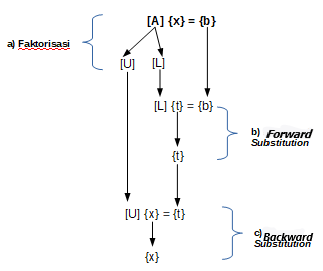
\includegraphics[width=0.9\linewidth]{./images/LU} 

}

\caption{Tahapan dekomposisi LU.}\label{fig:LUfig}
\end{figure}

Dekomposisi LU didasarkan pada operasi baris elementer. Pertama, kita perlu menemukan matriks segitiga atas yang sesuai dengan matriks \(A\). Solusi untuk melakukan dekomposisi bisa jadi tak terhingga, namun solusi yang paling sederhana adalah mengubah matriks \(A\) menjadi matriks \emph{row echelon form}. Kedua, \(L\) harus menjadi matriks segitiga bawah yang mereduksi ke-\(l\) dengan mengikuti operasi baris yang sama yag menghasilkan \(U\). Kita dapat menggunakan algoritma Doolittle untuk menghasilkan \(L\), di mana nilai setiap entri dalam matriks segitiga bawah merupakan pengali yang digunakan untuk menghilangkan entri yang sesuai untuk setiap proses \emph{row replacement}.

Pada praktiknya, proses eliminasi Gauss untuk memperoleh matriks \(U\) kadang menghasilkan nol di kolom pivotnya. Kondisi tersebut mengharuskan kita untuk melakukan proses \emph{row swapping} atau pertukaran baris (biasanya dengan baris bawahnya) untuk pivot bukan nol. Jika proses tersebut berhasil dilakukan bisa jadi matriks \(A\) mungkin setara dengan matriks LU, tetapi tidak sama dalam hal urutan nilai pada tiap barisnya. Agar kita dapat memperoleh hasil yang sama (matriks A sama dengan matriks LU), diperlukan matriks ketiga, \(P\). Matriks ini merupakan matriks identitas dengan ukuran sama dengan matriks \(A\). Jika pertukaran baris dilakukan selama proses pembentukan matriks \(U\), maka pertukaran baris yang sama juga akan diimplemenntasikan pada matriks \(P\). oleh karena itu, dalam praktiknya matriks \(A=PLU\) dan perkalian dengan matriks \(P\) berfungsi untuk mengembalikan urutan baris.

\begin{example}
\protect\hypertarget{exm:LUexmp}{}\label{exm:LUexmp}Selesaikan sistem persamaan linier berikut menggunakan faktorisasi LU
\end{example}

\[
\begin{matrix}
  x_1+x_2+3x_4=4 \\
  2x_1+x_2-x_3+x_4=1 \\
  3x_1-x_2-x_3+2x_4=-3 \\
  -x_1-2x_2+3x_3-x_4=4
\end{matrix}
\]

\textbf{Jawab}:

Nayatakan sistem persamaan tersebut ke dalam bentuk matriks \(Ax=b\).

\begin{equation*}
Ux=
\begin{bmatrix}
     1       & 1       & 0       & 3           \\[0.3em]
     2       & 1       & -1      & 1           \\[0.3em]
     3       & -1      & -1      & 2           \\[0.3em]
     -1      & 2       & 3       & -1           
     \end{bmatrix}
\begin{bmatrix}
     x_1                                          \\[0.3em]
     x_2                                          \\[0.3em]
     x_3                                          \\[0.3em]
     x_4                                       
     \end{bmatrix}
= \begin{bmatrix}
     4                                          \\[0.3em]
     1                                          \\[0.3em]
     -3                                          \\[0.3em]
     4                                       
     \end{bmatrix}
\end{equation*}

Lakukan operasi baris elementer pada matriks \(A\) untuk memperoleh matriks \(U\). Urutan operasi baris elementer yang dilakukan adalah sebagai berikut:

\begin{itemize}
\tightlist
\item
  \(\left(B_2-2B_1\right)\to B_2 \to l_{2,1}=2\),
\item
  \(\left(B_3-3B_1\right)\to B_3 \to l_{3,1}=3\),
\item
  \(\left(B_4+B_1\right)\to B_4 \to l_{4,1}=-1\),
\item
  \(\left(B_3-4B_2\right)\to B_3\to l_{3,2}=4\),
\item
  \(\left(B_4+3B_2\right)\to B_4 \to l_{4,2}=-3\),
\item
  \(l_{4,3}=0\)
\end{itemize}

Simpan pengali tiap tahapan pada masing-masing elemen matriks \(L\). Hasil operasi tersebut akan menghasilkan matriks triangular \(U\).

\[
U=
\begin{bmatrix}
     1       & 1       & 0       & 3           \\[0.3em]
     0       & -1      & -1      & -5          \\[0.3em]
     0       & 0       & 3       & 13          \\[0.3em]
     0       & 0       & 0       & -13           
\end{bmatrix}
\]

Untuk matriks \(L\) sebagai berikut:

\[
L=
\begin{bmatrix}
     1         & 0       & 0       & 0           \\[0.3em]
     2         & 1       & 0       & 0           \\[0.3em]
     3         & 4       & 1       & 0           \\[0.3em]
     -1        & -3      & 0       & 1           
\end{bmatrix}
\]

Karena pada proses operasi baris elementer tidak terdapat operasi pertukaran baris, maka matriks \(P\) tidak mengalami perubahan:

\[
P=
\begin{bmatrix}
     1         & 0       & 0       & 0           \\[0.3em]
     0         & 1       & 0       & 0           \\[0.3em]
     0         & 0       & 1       & 0           \\[0.3em]
     0         & 0       & 0       & 1           
     \end{bmatrix}
\]

Lakukan operasi \emph{forward substitution} menggunakan Persamaan \eqref{eq:LUdecomp5}.

\begin{equation*}
\begin{bmatrix}
      1         & 0       & 0       & 0           \\[0.3em]
      2         & 1       & 0       & 0           \\[0.3em]
      3         & 4       & 1       & 0           \\[0.3em]
      -1        & -3      & 0       & 1
     \end{bmatrix}
\begin{bmatrix}
     t_1                                          \\[0.3em]
     t_2                                          \\[0.3em]
     t_3                                          \\[0.3em]
     t_4                                       
     \end{bmatrix}
= \begin{bmatrix}
     4                                          \\[0.3em]
     1                                          \\[0.3em]
     -3                                          \\[0.3em]
     4                                       
     \end{bmatrix}
\end{equation*}

Berdasarkan hasil perhitungan diperoleh nilai vektor \(t\).

\[
t_1=4, t_2=1, t_3=-3, t_4=4
\]

Operasi terakhir yang perlu dilakukan untuk memperoleh nilai \(x\) adalah dengan melakukan \emph{backward substitution} menggunakan nilai vektor \(t\) yang telah dihitung.

\begin{equation*}
\begin{bmatrix}
     1       & 1       & 0       & 3           \\[0.3em]
     0       & -1      & -1      & -5          \\[0.3em]
     0       & 0       & 3       & 13          \\[0.3em]
     0       & 0       & 0       & -13
     \end{bmatrix}
\begin{bmatrix}
     x_1                                          \\[0.3em]
     x_2                                          \\[0.3em]
     x_3                                          \\[0.3em]
     x_4                                       
     \end{bmatrix}
= \begin{bmatrix}
     4                                          \\[0.3em]
     7                                          \\[0.3em]
     13                                          \\[0.3em]
     -13                      
     \end{bmatrix}
\end{equation*}

Berdasarkan hasil perhitungan diperoleh nilai \(x\) sebagai berikut:

\[
x_1=-1, x_2=2, x_3=0, x_4=1
\]

\begin{center}\rule{0.5\linewidth}{0.5pt}\end{center}

\textbf{Algoritma Dekomposisi LU}

\begin{enumerate}
\def\labelenumi{\arabic{enumi}.}
\tightlist
\item
  Masukkan matriks \(A\), dan vektor \(B\) beserta ukurannya \(n\)
\item
  Lakukan langkah poin ke-4 s/d poin 5 untuk meperoleh matriks \(U\).
\item
  Untuk baris ke-\(i\) di mana \(i=1\) s/d \(n\), perhatikan apakah nilai \(a_{i,j}\) sama dengan nol.
\end{enumerate}

\begin{itemize}
\tightlist
\item
  \textbf{Bila iya}, lakukan \emph{row swapping} antara baris ke-\(i\) dan baris ke-\(i+k\leq n\), dimana \(a_{i+k,j}\) tidak sama dengan nol. Bila tidak ada berarti perhitungan tidak bisa dilanjutkan dan proses dihentikan dengan tanpa penyelesaian.
\item
  \textbf{Bila tidak}, lanjutkan.
\end{itemize}

\begin{enumerate}
\def\labelenumi{\arabic{enumi}.}
\setcounter{enumi}{4}
\tightlist
\item
  Untuk baris ke-\(j\), dimana \(j=i+1\) s/d \(n\), lakukan operasi baris elementer:
\end{enumerate}

\begin{itemize}
\tightlist
\item
  Hitung \(c=\frac{a_{j,i}}{a_{i,i}}\)
\item
  untuk kolom \(k\), dimana \(k=1\) s/d \(n+1\), hitung \(a_{j,k}=a_{j,k}-c_i.a_{i,k}\)
\end{itemize}

\begin{enumerate}
\def\labelenumi{\arabic{enumi}.}
\setcounter{enumi}{5}
\tightlist
\item
  Lakukan langkah poin ke-7 s/d poin 9 untuk memperoleh matriks \(L\)
\item
  Untuk diagonal matriks \(L\) isikan dengan nilai 1 dan elemen di atas diagonal dengan nilai nol.
\item
  Untuk elemen di bawah diagonal isikan dengan faktor pengali operasi baris elementer matriks \(U\).
\item
  Lakukan proses \emph{forward substitution} menggunakan Persamaan \eqref{eq:LUdecomp6} untuk memperoleh nilai vektor \(t\).
\item
  Lakukan \emph{backward substituion} menggunakan Persamaan \eqref{eq:refsolution}.
\end{enumerate}

\begin{center}\rule{0.5\linewidth}{0.5pt}\end{center}

Berdasarkan algoritma tersebut, kita dapat menyusun algoritma faktorisasi LU menggunakan \texttt{R}. Berikut adalah sintaks yang digunakan:

\begin{Shaded}
\begin{Highlighting}[]
\NormalTok{lu\_solve }\OtherTok{\textless{}{-}} \ControlFlowTok{function}\NormalTok{(a, }\AttributeTok{b=}\ConstantTok{NULL}\NormalTok{)\{}
\NormalTok{    m }\OtherTok{\textless{}{-}} \FunctionTok{nrow}\NormalTok{(a)}
\NormalTok{    n }\OtherTok{\textless{}{-}} \FunctionTok{ncol}\NormalTok{(a)}
\NormalTok{    piv }\OtherTok{\textless{}{-}} \DecValTok{1}

\CommentTok{\# membentuk matriks identitas P dan L}
\NormalTok{    P }\OtherTok{\textless{}{-}}\NormalTok{ L }\OtherTok{\textless{}{-}} \FunctionTok{diag}\NormalTok{(n)}

\CommentTok{\# cek elemen diagonal utama apakah bernilai nol}
    \ControlFlowTok{for}\NormalTok{(row\_curr }\ControlFlowTok{in} \DecValTok{1}\SpecialCharTok{:}\NormalTok{m)\{}
        \ControlFlowTok{if}\NormalTok{(piv }\SpecialCharTok{\textless{}=}\NormalTok{ n)\{}
\NormalTok{            i }\OtherTok{\textless{}{-}}\NormalTok{ row\_curr}
            \ControlFlowTok{while}\NormalTok{(a[i, piv] }\SpecialCharTok{==} \DecValTok{0} \SpecialCharTok{\&\&}\NormalTok{ i }\SpecialCharTok{\textless{}}\NormalTok{ m)\{}
\NormalTok{                i }\OtherTok{\textless{}{-}}\NormalTok{ i }\SpecialCharTok{+} \DecValTok{1}
                \ControlFlowTok{if}\NormalTok{(i }\SpecialCharTok{\textgreater{}}\NormalTok{ m)\{}
\NormalTok{                    i }\OtherTok{\textless{}{-}}\NormalTok{ row\_curr}
\NormalTok{                    piv }\OtherTok{\textless{}{-}}\NormalTok{ piv }\SpecialCharTok{+} \DecValTok{1}
                    \ControlFlowTok{if}\NormalTok{(piv }\SpecialCharTok{\textgreater{}}\NormalTok{ n)}
                        \FunctionTok{return}\NormalTok{(}\FunctionTok{list}\NormalTok{(}\AttributeTok{P =}\NormalTok{ P, }\AttributeTok{L =}\NormalTok{ L, }\AttributeTok{U =}\NormalTok{ a))}
\NormalTok{                \}}
\NormalTok{            \}}
            
\CommentTok{\# jika elemen diagonal utama bernilai nol,lakukan row swapping}
            \ControlFlowTok{if}\NormalTok{(i }\SpecialCharTok{!=}\NormalTok{ row\_curr)\{}
\NormalTok{                a }\OtherTok{\textless{}{-}} \FunctionTok{swap\_row}\NormalTok{(a, i, row\_curr)}
\NormalTok{                P }\OtherTok{\textless{}{-}} \FunctionTok{swap\_row}\NormalTok{(P, i, row\_curr)}
\NormalTok{            \}}
            
  \CommentTok{\# pembentukan matriks L dan U}
            \ControlFlowTok{for}\NormalTok{(j }\ControlFlowTok{in}\NormalTok{ row\_curr}\SpecialCharTok{:}\NormalTok{m)}
                \ControlFlowTok{if}\NormalTok{(j }\SpecialCharTok{!=}\NormalTok{ row\_curr)\{}
\NormalTok{                    k }\OtherTok{\textless{}{-}}\NormalTok{ a[j, piv]}\SpecialCharTok{/}\NormalTok{a[row\_curr, piv]}
                    
  \CommentTok{\# matriks U}
\NormalTok{                    a }\OtherTok{\textless{}{-}} \FunctionTok{replace\_row}\NormalTok{(a, row\_curr, j, }\SpecialCharTok{{-}}\NormalTok{k)}
                    
  \CommentTok{\# pengisian elemen matriks L}
\NormalTok{                    L[j, piv] }\OtherTok{\textless{}{-}}\NormalTok{ k}
\NormalTok{                \}}
\NormalTok{            piv }\OtherTok{\textless{}{-}}\NormalTok{ piv }\SpecialCharTok{+} \DecValTok{1}
\NormalTok{        \}}
\NormalTok{    \}}
    
\CommentTok{\# penyelesaian persamaan linier}
    \ControlFlowTok{if}\NormalTok{(}\FunctionTok{is.null}\NormalTok{(b))\{}
      \FunctionTok{return}\NormalTok{(}\FunctionTok{list}\NormalTok{(}\AttributeTok{P =}\NormalTok{ P, }\AttributeTok{L =}\NormalTok{ L, }\AttributeTok{U =}\NormalTok{ a))}
\NormalTok{    \}}\ControlFlowTok{else}\NormalTok{\{}
      
      \CommentTok{\# forward substitution}
\NormalTok{      t }\OtherTok{\textless{}{-}} \FunctionTok{forwardsolve}\NormalTok{(L, b)}
      
      \CommentTok{\# backward substitution}
\NormalTok{      x }\OtherTok{\textless{}{-}} \FunctionTok{backsolve}\NormalTok{(a, t)}
      \FunctionTok{return}\NormalTok{(}\FunctionTok{list}\NormalTok{(}\AttributeTok{P =}\NormalTok{ P, }\AttributeTok{L =}\NormalTok{ L, }\AttributeTok{U =}\NormalTok{ a, }\AttributeTok{result=}\NormalTok{x))}
\NormalTok{     \}}
\NormalTok{\}}
\end{Highlighting}
\end{Shaded}

Kita dapat menyelesaikan sistem persamaan linier pada Contoh \ref{exm:LUexmp} menggunakan fungsi yang telah kita buat.

\begin{Shaded}
\begin{Highlighting}[]
\CommentTok{\# membuat matriks a dan vektor b}
\NormalTok{a }\OtherTok{\textless{}{-}} \FunctionTok{matrix}\NormalTok{(}\FunctionTok{c}\NormalTok{(}\DecValTok{1}\NormalTok{,}\DecValTok{2}\NormalTok{,}\DecValTok{3}\NormalTok{,}\SpecialCharTok{{-}}\DecValTok{1}\NormalTok{,}\DecValTok{1}\NormalTok{,}\DecValTok{1}\NormalTok{,}\SpecialCharTok{{-}}\DecValTok{1}\NormalTok{,}\DecValTok{2}\NormalTok{,}
              \DecValTok{0}\NormalTok{,}\SpecialCharTok{{-}}\DecValTok{1}\NormalTok{,}\SpecialCharTok{{-}}\DecValTok{1}\NormalTok{,}\DecValTok{3}\NormalTok{,}\DecValTok{3}\NormalTok{,}\DecValTok{1}\NormalTok{,}\DecValTok{2}\NormalTok{,}\SpecialCharTok{{-}}\DecValTok{1}\NormalTok{),}
            \AttributeTok{nrow=}\DecValTok{4}\NormalTok{)}
\NormalTok{b }\OtherTok{\textless{}{-}} \FunctionTok{c}\NormalTok{(}\DecValTok{4}\NormalTok{,}\DecValTok{1}\NormalTok{,}\SpecialCharTok{{-}}\DecValTok{3}\NormalTok{,}\DecValTok{4}\NormalTok{)}

\CommentTok{\# penyelesaian}
\NormalTok{decomp}\OtherTok{\textless{}{-}}\FunctionTok{lu\_solve}\NormalTok{(a,b)}
\end{Highlighting}
\end{Shaded}

Untuk membentuk kembali matriks \(A\), kita dapat mengalikan matriks \(L\), \(U\), dan \(P\).

\begin{Shaded}
\begin{Highlighting}[]
\NormalTok{decomp}\SpecialCharTok{$}\NormalTok{L}\SpecialCharTok{\%*\%}\NormalTok{decomp}\SpecialCharTok{$}\NormalTok{U}\SpecialCharTok{\%*\%}\NormalTok{decomp}\SpecialCharTok{$}\NormalTok{P}
\end{Highlighting}
\end{Shaded}

\begin{verbatim}
##      [,1] [,2] [,3] [,4]
## [1,]    1    1    0    3
## [2,]    2    1   -1    1
## [3,]    3   -1   -1    2
## [4,]   -1    2    3   -1
\end{verbatim}

\begin{example}
\protect\hypertarget{exm:LUexmp2}{}\label{exm:LUexmp2}Lakukan dekomposisi LU pada matriks berikut dan lakukan pengecekan apakah perkalian hasil dekomposisi matriks akan menghasilkan matriks semula!
\end{example}

\[
\begin{bmatrix}
     0         & 1       & -1                  \\[0.3em]
     1         & 5       & 9                   \\[0.3em]
     7         & -1      & -5                  
\end{bmatrix}
\]

\textbf{Jawab}:

Lakukan proses dekomposisi menggunakan fungsi \texttt{lu\_solve()}.

\begin{Shaded}
\begin{Highlighting}[]
\CommentTok{\# membentuk matriks a}
\NormalTok{(A }\OtherTok{\textless{}{-}} \FunctionTok{matrix}\NormalTok{(}\FunctionTok{c}\NormalTok{(}\DecValTok{0}\NormalTok{, }\DecValTok{1}\NormalTok{, }\DecValTok{7}\NormalTok{, }\DecValTok{1}\NormalTok{, }\DecValTok{5}\NormalTok{, }\SpecialCharTok{{-}}\DecValTok{1}\NormalTok{, }\SpecialCharTok{{-}}\DecValTok{2}\NormalTok{, }\DecValTok{9}\NormalTok{, }\SpecialCharTok{{-}}\DecValTok{5}\NormalTok{), }\DecValTok{3}\NormalTok{))}
\end{Highlighting}
\end{Shaded}

\begin{verbatim}
##      [,1] [,2] [,3]
## [1,]    0    1   -2
## [2,]    1    5    9
## [3,]    7   -1   -5
\end{verbatim}

\begin{Shaded}
\begin{Highlighting}[]
\CommentTok{\# dekomposisi lu}
\NormalTok{decomp}\OtherTok{\textless{}{-}}\FunctionTok{lu\_solve}\NormalTok{(A)}
\end{Highlighting}
\end{Shaded}

Lakukan pengecekan apakah matriks hasil dekomposisi akan menghasilkan matriks \(A\).

\begin{Shaded}
\begin{Highlighting}[]
\NormalTok{decomp}\SpecialCharTok{$}\NormalTok{P }\SpecialCharTok{\%*\%}\NormalTok{ decomp}\SpecialCharTok{$}\NormalTok{L }\SpecialCharTok{\%*\%}\NormalTok{ decomp}\SpecialCharTok{$}\NormalTok{U}
\end{Highlighting}
\end{Shaded}

\begin{verbatim}
##      [,1] [,2] [,3]
## [1,]    0    1   -2
## [2,]    1    5    9
## [3,]    7   -1   -5
\end{verbatim}

Fungsi \texttt{lu()} pada Paket \texttt{Matrix} dapat digunakan untuk melakukan dekomposisi LU. Untuk meggunakan fungsi tersebut, kita harus menginstall dan mengaktifkan Paket \texttt{Matrix}.

\begin{Shaded}
\begin{Highlighting}[]
\FunctionTok{install.packages}\NormalTok{(}\StringTok{"Matrix"}\NormalTok{)}
\end{Highlighting}
\end{Shaded}

\begin{Shaded}
\begin{Highlighting}[]
\FunctionTok{library}\NormalTok{(Matrix)}
\end{Highlighting}
\end{Shaded}

Untuk dapat menggunakannya kita hanya perlu menginputkan matriks kedalam fungsi tersebut. Berikut adalah contoh penerapannya:

\begin{Shaded}
\begin{Highlighting}[]
\CommentTok{\# membuat matriks a }
\NormalTok{a }\OtherTok{\textless{}{-}}\NormalTok{ Matrix}\SpecialCharTok{::}\FunctionTok{Matrix}\NormalTok{(}\FunctionTok{round}\NormalTok{(}\FunctionTok{rnorm}\NormalTok{(}\DecValTok{9}\NormalTok{),}\DecValTok{2}\NormalTok{), }\AttributeTok{nrow=}\DecValTok{3}\NormalTok{)}

\CommentTok{\# dekomposisi}
\NormalTok{lum }\OtherTok{\textless{}{-}}\NormalTok{ Matrix}\SpecialCharTok{::}\FunctionTok{lu}\NormalTok{(a)}
\NormalTok{lum}
\end{Highlighting}
\end{Shaded}

\begin{verbatim}
## 'MatrixFactorization' of Formal class 'denseLU' [package "Matrix"] with 4 slots
##   ..@ Dimnames:List of 2
##   .. ..$ : NULL
##   .. ..$ : NULL
##   ..@ x       : num [1:9] -0.95 0.705 0.589 0.53 -0.604 ...
##   ..@ perm    : int [1:3] 2 3 3
##   ..@ Dim     : int [1:2] 3 3
\end{verbatim}

Untuk menampilkan hasil dekomposisi, jalankan fungsi \texttt{expand()}.

\begin{Shaded}
\begin{Highlighting}[]
\NormalTok{decomp }\OtherTok{\textless{}{-}}\NormalTok{ Matrix}\SpecialCharTok{::}\FunctionTok{expand}\NormalTok{(lum)}
\NormalTok{decomp}
\end{Highlighting}
\end{Shaded}

\begin{verbatim}
## $L
## 3 x 3 Matrix of class "dtrMatrix" (unitriangular)
##      [,1]    [,2]    [,3]   
## [1,]  1.0000       .       .
## [2,]  0.7053  1.0000       .
## [3,]  0.5895 -0.2279  1.0000
## 
## $U
## 3 x 3 Matrix of class "dtrMatrix"
##      [,1]    [,2]    [,3]   
## [1,] -0.9500  0.5300  1.7600
## [2,]       . -0.6038 -0.7513
## [3,]       .       .  0.1913
## 
## $P
## 3 x 3 sparse Matrix of class "pMatrix"
##           
## [1,] . . |
## [2,] | . .
## [3,] . | .
\end{verbatim}

\hypertarget{dekomposisi-cholesky}{%
\subsection{Dekomposisi Cholesky}\label{dekomposisi-cholesky}}

Dekomposisi Cholesky memberikan faktorisasi matriks alternatif sehingga \(A = LL^T\), di mana \(L^T\) merupakan transpose konjugat dari matriks \(L\). Dalam kasus ini, penulis hanya bekerja dengan matriks rill dengan nilai rill dan bagian imajiner nol. Jadi untuk tujuan \emph{sub-chapter} ini, matriks \(L^T\) hanyalah transpose dari matriks \(L\).

Seperti dekomposisi LU, dekomposisi Cholesky dapat digunakan untuk menyelesaikan sistem persamaan linier. Kelebihannya, Menemukan dekomposisi Cholesky jauh lebih cepat daripada dekomposisi LU. Namun, dekomposisi ini hanya terbatas pada matriks tertentu saja. Dekomposisi Cholesky hanya dapat digunakan pada matriks definit positif dan simetris. Matriks simeteris merupakan matriks yang nilai di atas dan di bawah diagonalnya simetris atau sama; secara matematis, untuk semua \(i\) dan \(j\) pada matriks \(A\), \(a_{i;j}=a_{j;i}\). Definit positif berarti bahwa setiap entri pivot (nilai elemen diagonal utama) selelu bernilai positif. Selain itu, untuk matriks definit positif, hubungan \(xAx>0\) untuk semua vektor, \(x\).

Karena \(L^∗\) transpose dari matriks \(L\), maka \(l^{T}_{i,j} = l_{j,i}\) untuk semua nilai \(i\) dan \(j\). Tanpa kendala (\emph{constraint}) ini, dekomposisi Cholesky akan mirip dekomposisi LU. Tetapi dengan kendala ini, nilai elemen matriks \(L\) dan \(L^T\) harus dipilih dengan cermat sehingga hubungan \(A = LL^T\) berlaku. Bentuk dekomposisi Cholesky disajikan pada Persamaan \eqref{eq:cholesky}.

\begin{equation}
\begin{bmatrix}
     a_{1,1} & a_{1,2} & a_{1,3} &\cdots& a_{1,m}           \\[0.3em]
     a_{2,1} & a_{2,2} & a_{2,3} &\cdots& a_{2,m}           \\[0.3em]
     a_{3,1} & a_{3,2} & a_{3,3} &\cdots& a_{3,m}           \\[0.3em]
     \vdots  & \vdots  & \vdots  &\ddots& \vdots            \\[0.3em]
     a_{m,1} & a_{m,2} & a_{m,3} &\cdots& a_{m,m}
     \end{bmatrix}
=
\begin{bmatrix}
     l_{1,1} & 0       & 0       &\cdots& 0           \\[0.3em]
     l_{2,1} & l_{2,2} & 0       &\cdots& 0           \\[0.3em]
     l_{3,1} & l_{3,2} & l_{3,3} &\cdots& 0           \\[0.3em]
     \vdots  & \vdots  & \vdots  &\ddots& \vdots            \\[0.3em]
     l_{m,1} & l_{m,2} & l_{m,3} &\cdots& l_{m,m}
     \end{bmatrix}
\begin{bmatrix}
     l_{1,1} & l_{1,2} & l_{1,3} &\cdots& l_{1,m}           \\[0.3em]
     0       & l_{2,2} & l_{2,3} &\cdots& l_{2,m}           \\[0.3em]
     0       & 0       & l_{3,3} &\cdots& l_{3,m}           \\[0.3em]
     \vdots  & \vdots  & \vdots  &\ddots& \vdots            \\[0.3em]
     0       & 0       & 0       &\cdots& l_{m,m}
     \end{bmatrix}
  \label{eq:cholesky}
\end{equation}

Untuk setiap elemen matriks \(A\) memiliki hubungan yang dituliskan pada Persamaan \eqref{eq:cholesky2}.

\begin{equation}
a_{i,j}=\sum_{k=1}^mL_{i,k}L_{k,j}
  \label{eq:cholesky2}
\end{equation}

Berdasarkan Persamaan \eqref{eq:cholesky}, sejumlah nilai elemen \(L_{i,k}\) dan \(L_{k,j}\) adalah nol. Nilai tiap elemen diagonal utama yang tidak bernilai nol dihitung menggunakan Persamaan \eqref{eq:cholesky3}.

\begin{equation}
l_{i,i}=\sqrt{\left(a_{i,i}-\sum_{k=1}^{i-1}l_{i,k}^2\right)}
  \label{eq:cholesky3}
\end{equation}

Elemen diagonal dihitung menggunakan Persamaan \eqref{eq:cholesky5}

\begin{equation}
l_{i,j}=\frac{1}{l_{i,i}}\left(a_{i,j}-\sum_{k=1}^{i-1}l_{i,k}l_{j,k}\right)
  \label{eq:cholesky5}
\end{equation}

\begin{center}\rule{0.5\linewidth}{0.5pt}\end{center}

\textbf{Algoritma Dekomposisi Cholesky}

\begin{enumerate}
\def\labelenumi{\arabic{enumi}.}
\tightlist
\item
  Masukkan matriks \(A\), dan vektor \(B\) beserta ukurannya \(n\).
\item
  Untuk elemen matriks \(L\), hitung menggunakan Persamaan \eqref{eq:cholesky5}.
\item
  Untuk nilai diagonal utama matriks \(L\), hitung menggunakan Persamaan \eqref{eq:cholesky3}.
\item
  Untuk memperoleh matriks \(L^T\), lakukan transpose pada matriks \(L\).
\item
  Untuk memperoleh nilai \(x\),
\end{enumerate}

\begin{itemize}
\tightlist
\item
  Hitung vektor \(t\) menggunakan Persamaan \eqref{eq:LUdecomp4}.
\item
  Hitung vektor \(x\) menggunakan Persamaan \eqref{eq:LUdecomp3}, dimana matriks \(U=L^T\).
\end{itemize}

\begin{center}\rule{0.5\linewidth}{0.5pt}\end{center}

Berdasarkan algoritma tersebut, kita dapat menyusun fungsi pada \texttt{R} untuk melakukan dekomposisi Cholesky. Fungsi tersebut disajikan pada sintaks berikut:

\begin{Shaded}
\begin{Highlighting}[]
\NormalTok{cholesky\_solve }\OtherTok{\textless{}{-}} \ControlFlowTok{function}\NormalTok{(a, }\AttributeTok{b=}\ConstantTok{NULL}\NormalTok{)\{}
\NormalTok{    m }\OtherTok{\textless{}{-}} \FunctionTok{nrow}\NormalTok{(a)}
   
\CommentTok{\# membentuk matriks L dengan elemen nol}
\NormalTok{    L }\OtherTok{=} \FunctionTok{diag}\NormalTok{(}\DecValTok{0}\NormalTok{,m)}

\CommentTok{\# Perhitungan elemen matriks L}
    \ControlFlowTok{for}\NormalTok{(i }\ControlFlowTok{in} \DecValTok{1}\SpecialCharTok{:}\NormalTok{m)\{}
        \ControlFlowTok{for}\NormalTok{(k }\ControlFlowTok{in} \DecValTok{1}\SpecialCharTok{:}\NormalTok{i)\{}
\NormalTok{            p\_sum }\OtherTok{\textless{}{-}} \DecValTok{0}
            \ControlFlowTok{for}\NormalTok{(j }\ControlFlowTok{in} \DecValTok{1}\SpecialCharTok{:}\NormalTok{k)}
\NormalTok{                p\_sum }\OtherTok{\textless{}{-}}\NormalTok{ p\_sum }\SpecialCharTok{+}\NormalTok{ L[j,i]}\SpecialCharTok{*}\NormalTok{L[j,k]}
                
\CommentTok{\# Pehitungan elemen diagonal utama}
            \ControlFlowTok{if}\NormalTok{(i}\SpecialCharTok{==}\NormalTok{k)}
\NormalTok{                L[k,i]}\OtherTok{\textless{}{-}}\FunctionTok{sqrt}\NormalTok{(a[i,i]}\SpecialCharTok{{-}}\NormalTok{p\_sum)}
            \ControlFlowTok{else}
\NormalTok{                L[k,i]}\OtherTok{\textless{}{-}}\NormalTok{(a[k,i]}\SpecialCharTok{{-}}\NormalTok{p\_sum)}\SpecialCharTok{/}\NormalTok{L[k,k]}
\NormalTok{        \}}
\NormalTok{    \}}
    
\CommentTok{\# Perhitungan elemn matriks L*}
\NormalTok{    tL }\OtherTok{\textless{}{-}} \FunctionTok{t}\NormalTok{(L)}
    
\CommentTok{\# penyelesaian persamaan linier}
    \ControlFlowTok{if}\NormalTok{(}\FunctionTok{is.null}\NormalTok{(b))\{}
      \FunctionTok{return}\NormalTok{(}\FunctionTok{list}\NormalTok{(}\AttributeTok{L =}\NormalTok{ L, }\AttributeTok{tL =}\NormalTok{ tL, }\AttributeTok{a =}\NormalTok{ a))}
\NormalTok{    \}}\ControlFlowTok{else}\NormalTok{\{}
      
      \CommentTok{\# forward substitution}
\NormalTok{      t }\OtherTok{\textless{}{-}} \FunctionTok{forwardsolve}\NormalTok{(L, b)}
      
      \CommentTok{\# backward substitution}
\NormalTok{      x }\OtherTok{\textless{}{-}} \FunctionTok{backsolve}\NormalTok{(tL, t)}
      \FunctionTok{return}\NormalTok{(}\FunctionTok{list}\NormalTok{(}\AttributeTok{L =}\NormalTok{ L, }\AttributeTok{tL =}\NormalTok{ tL, }\AttributeTok{a =}\NormalTok{ a, }\AttributeTok{result=}\NormalTok{x))}
\NormalTok{     \}}
\NormalTok{\}}
\end{Highlighting}
\end{Shaded}

\begin{example}
\protect\hypertarget{exm:cholexm2}{}\label{exm:cholexm2}Dengan menggunakan fungsi \texttt{cholesky\_solve()}, lakukan dekomposisi pada matriks berikut! Lakukan pengecekan pada hasil dekomposisi apakah hasil kali matriks dekomposisi akan menghasilkan matriks semula!
\end{example}

\[
\begin{bmatrix}
     9         & -3       & 6                  \\[0.3em]
     -3         & 17       & -10                   \\[0.3em]
     6         & -10      & 12                  
\end{bmatrix}
\]

\textbf{Jawab}:

Dekomposisi Cholesky menggunakan fungsi \texttt{cholesky\_solve()}, disajikan pada sintaks berikut:

\begin{Shaded}
\begin{Highlighting}[]
\NormalTok{a }\OtherTok{\textless{}{-}} \FunctionTok{matrix}\NormalTok{(}\FunctionTok{c}\NormalTok{(}\DecValTok{9}\NormalTok{,}\SpecialCharTok{{-}}\DecValTok{3}\NormalTok{,}\DecValTok{6}\NormalTok{,}\SpecialCharTok{{-}}\DecValTok{3}\NormalTok{,}\DecValTok{17}\NormalTok{,}\SpecialCharTok{{-}}\DecValTok{10}\NormalTok{,}\DecValTok{6}\NormalTok{,}\SpecialCharTok{{-}}\DecValTok{10}\NormalTok{,}\DecValTok{12}\NormalTok{),}\DecValTok{3}\NormalTok{)}

\CommentTok{\# dekomposisi Cholesky}
\NormalTok{(decomp}\OtherTok{\textless{}{-}}\FunctionTok{cholesky\_solve}\NormalTok{(a))}
\end{Highlighting}
\end{Shaded}

\begin{verbatim}
## $L
##      [,1] [,2] [,3]
## [1,]    3   -1    2
## [2,]    0    4   -2
## [3,]    0    0    2
## 
## $tL
##      [,1] [,2] [,3]
## [1,]    3    0    0
## [2,]   -1    4    0
## [3,]    2   -2    2
## 
## $a
##      [,1] [,2] [,3]
## [1,]    9   -3    6
## [2,]   -3   17  -10
## [3,]    6  -10   12
\end{verbatim}

\begin{Shaded}
\begin{Highlighting}[]
\CommentTok{\# mengecek hasil dekomposisi}
\NormalTok{decomp}\SpecialCharTok{$}\NormalTok{tL }\SpecialCharTok{\%*\%}\NormalTok{ decomp}\SpecialCharTok{$}\NormalTok{L}
\end{Highlighting}
\end{Shaded}

\begin{verbatim}
##      [,1] [,2] [,3]
## [1,]    9   -3    6
## [2,]   -3   17  -10
## [3,]    6  -10   12
\end{verbatim}

Fungsi lain yang dapat digunakan untuk melakukan dekomposisi Cholesky adalah menggunakan fungsi \texttt{chol()} pada Paket \texttt{Matrix}. Pada fungsi tersebut, kita hanya perlu menginputkan objek matrik kedalamnya. Berikut adalah contoh penerapan fungsi tersebut menggunakan matriks pada Contoh \ref{exm:cholexm2}.

\begin{Shaded}
\begin{Highlighting}[]
\FunctionTok{chol}\NormalTok{(a)}
\end{Highlighting}
\end{Shaded}

\begin{verbatim}
##      [,1] [,2] [,3]
## [1,]    3   -1    2
## [2,]    0    4   -2
## [3,]    0    0    2
\end{verbatim}

\begin{quote}
\textbf{Penting!!!}

Fungsi \texttt{chol()} hanya menampilkan matriks \(L^T\). Untuk menampilkan matriks \(L\), kita perlu melakukan transpose
\end{quote}

\hypertarget{othersdecomp}{%
\subsection{Dekomposisi Lainnya}\label{othersdecomp}}

Terdapat beberapa algoritma lain yang telah dikembangkan untuk melakukan dekomposisi matriks. Pada buku ini hanya akan dijelaskan secara singkat terkait fungsi yang digunakan dalam melakukan dekomposisi matriks. Algoritma yang akan dijelaskan pada \emph{sub-chapter} ini antara lain: QR, \emph{singular value decomposition} (SVD), dan dekomposisi eigen. Untuk algoritma lainnya, pembaca dapat membaca buku terkait atau mengecek dokumentasinya pada Paket \texttt{base}.

\hypertarget{qrdecomp}{%
\subsubsection{Dekomposisi QR}\label{qrdecomp}}

Dekomposisi QR merupakan dekomposisi yang penting dalam menyelesaikan sistem persamaan linier. Dekomposisi ini juga berperan penting untuk menghitung koefisien regresi dan pengaplikasian algoritma Newton-Raphson.

Untuk memperoleh informasi terkait dekomposisi ini, pembaca dapat mengetikkan sintaks berikut pada \texttt{R}:

\begin{Shaded}
\begin{Highlighting}[]
\NormalTok{?qr}
\end{Highlighting}
\end{Shaded}

Berikut merupakan contoh penerapan fungsi \texttt{qr()} untuk menyelesaikan sistem persamaan linier:

\begin{Shaded}
\begin{Highlighting}[]
\CommentTok{\# membuat matriks A dan B}
\FunctionTok{set.seed}\NormalTok{(}\DecValTok{123}\NormalTok{)}
\NormalTok{A }\OtherTok{\textless{}{-}} \FunctionTok{matrix}\NormalTok{((}\DecValTok{1}\SpecialCharTok{:}\DecValTok{12}\NormalTok{)}\SpecialCharTok{+}\FunctionTok{rnorm}\NormalTok{(}\DecValTok{12}\NormalTok{), }\AttributeTok{nrow=}\DecValTok{4}\NormalTok{)}
\NormalTok{b }\OtherTok{\textless{}{-}} \DecValTok{2}\SpecialCharTok{:}\DecValTok{5}

\CommentTok{\# dekomposisi matriks A}
\FunctionTok{qr}\NormalTok{(A)}
\end{Highlighting}
\end{Shaded}

\begin{verbatim}
## $qr
##         [,1]     [,2]     [,3]
## [1,] -6.3778 -12.1257 -19.8501
## [2,]  0.2775  -6.3105  -7.9392
## [3,]  0.7148  -0.6461   2.3512
## [4,]  0.6382  -0.5654   0.2767
## 
## $rank
## [1] 3
## 
## $qraux
## [1] 1.069 1.513 1.961
## 
## $pivot
## [1] 1 2 3
## 
## attr(,"class")
## [1] "qr"
\end{verbatim}

\begin{Shaded}
\begin{Highlighting}[]
\CommentTok{\# memperoleh penyelesaian SPL}
\FunctionTok{qr.solve}\NormalTok{(A,b)}
\end{Highlighting}
\end{Shaded}

\begin{verbatim}
## [1]  0.3046 -0.1111  0.3237
\end{verbatim}

\hypertarget{svddecomp}{%
\subsubsection{\texorpdfstring{\emph{Singular Value Decomposition}}{Singular Value Decomposition}}\label{svddecomp}}

\emph{Singular value decomposition} (SVD) merupakan algoritma faktorisasi matriks yang mendekomposisi matriks segiempat menjadi matriks \(UDV_H\), dimana \(D\) merupakan mmatriks diagonal non negatif, \(U\) dan \(V\) merupakan matriks \emph{unitary}, dan \(V_H\) merupakan matriks tanspose konjugat dari matriks \(V\). Algoritma ini banyak digunakan dalam analisis \emph{principal component}.

Pada \texttt{R}, SVD dapat dilakukan menggunakan fungsi \texttt{svd()} dari Paket \texttt{base}. Berikut adalah sintaks untuk memperoleh informasi terkait fungsi tersebut:

\begin{Shaded}
\begin{Highlighting}[]
\NormalTok{?svd}
\end{Highlighting}
\end{Shaded}

Berikut adalah contoh penerapan fungsi \texttt{svd()}:

\begin{Shaded}
\begin{Highlighting}[]
\CommentTok{\# dekomposisi matriks A}
\FunctionTok{svd}\NormalTok{(A)}
\end{Highlighting}
\end{Shaded}

\begin{verbatim}
## $d
## [1] 26.094  2.727  1.330
## 
## $u
##         [,1]    [,2]    [,3]
## [1,] -0.3685 -0.5661  0.6651
## [2,] -0.4707 -0.5703 -0.6113
## [3,] -0.5740  0.4324 -0.2590
## [4,] -0.5596  0.4089  0.3419
## 
## $v
##         [,1]     [,2]    [,3]
## [1,] -0.2257  0.87169 -0.4350
## [2,] -0.5202 -0.48536 -0.7028
## [3,] -0.8237  0.06764  0.5630
\end{verbatim}

\hypertarget{eigendecomp}{%
\subsubsection{Dekomposisi Eigen}\label{eigendecomp}}

Proses umum yang digunakan untuk menemukan nilai eigen dan vektor eigen suatu matriks segiempat dapat dilihat sebagai proses dari dekomposisi eigen. Proses ini akan mendekomposisi matriks menjadi \(VDV^{-1}\), dimana \(D\) merupakan matriks diagonal yang terbentuk dari nilai eigen, dan \(V\) merupakan vektor eigen. Proses dekomposisi ini akan berguna bagi pembaca yang ingin mempelajari \emph{principal component analysis}.

Fungsi \texttt{eigen()} pada Paket \texttt{base} dapat digunakan untuk melakukan dekomposisi eigen. Untuk mempelajari lebih jauh terkait fungsi ini, pambaca dapat menjalankan sintaks berikut:

\begin{Shaded}
\begin{Highlighting}[]
\NormalTok{?eigen}
\end{Highlighting}
\end{Shaded}

Berikut adalah contoh sintaks untuk melakukan dekomposisi eigen:

\begin{Shaded}
\begin{Highlighting}[]
\NormalTok{A }\OtherTok{\textless{}{-}} \FunctionTok{matrix}\NormalTok{(}\FunctionTok{c}\NormalTok{(}\DecValTok{2}\NormalTok{,}\SpecialCharTok{{-}}\DecValTok{1}\NormalTok{,}\DecValTok{0}\NormalTok{,}\SpecialCharTok{{-}}\DecValTok{1}\NormalTok{,}\DecValTok{2}\NormalTok{,}\SpecialCharTok{{-}}\DecValTok{1}\NormalTok{,}\DecValTok{0}\NormalTok{,}\SpecialCharTok{{-}}\DecValTok{1}\NormalTok{,}\DecValTok{2}\NormalTok{), }\AttributeTok{nrow=}\DecValTok{3}\NormalTok{)}

\CommentTok{\# dekomposisi matriks A}
\FunctionTok{eigen}\NormalTok{(A)}
\end{Highlighting}
\end{Shaded}

\begin{verbatim}
## eigen() decomposition
## $values
## [1] 3.4142 2.0000 0.5858
## 
## $vectors
##         [,1]       [,2]   [,3]
## [1,] -0.5000 -7.071e-01 0.5000
## [2,]  0.7071  1.099e-15 0.7071
## [3,] -0.5000  7.071e-01 0.5000
\end{verbatim}

\hypertarget{iteratif}{%
\section{Metode Iterasi}\label{iteratif}}

Pada Chapter \ref{iteratif} kita akan membahas penyelesaian persamaan linier dengan menggunakan metode iterasi. Terdapat dua metode iterasi yang akan dibahas yaitu iterasi Jacobi dan Gauss-Seidel.

Metode iterasi dimulai dengan estimasi nilai akhir. Setelah menerapkan beberapa perlakuan pada nilai estimasi, hasil perlakuan selanjutnya menjadi nilai estimasi untuk iterasi berikutnya. Proses tersebut akan berlangsung secara terus-menerus hingga ambang batas dipenuhi. Nilai ambang batas dapat berupa jumlah iterasi maksimum atau selisih antara nilai estimasi baru dan estimasi semula lebih kecil dari suatu nilai toleransi yang ditetapkan.

Jumlah kuadrat merupakan metode yang sering digunakan untuk mengecek apakah selisih nilai estimasi baru terhadap estimasi lama lebih kecil dari nilai toleransi yang ditetapkan. Persamaan \eqref{eq:toleransi} menampilkan hubungan antara jumlah kuadrat dan nilai toleransi pada proses iterasi.

\begin{equation}
\sqrt{\sum_{i=1}^n\left(x_i^{n+1}-x_i^{n}\right)^2}<t_0
 \label{eq:toleransi}
\end{equation}

dimana \(x^{n}\) merupakan iterasi ke-\(n\) dari algoritma dan \(t_0\) merupakan nilai toleransi maksimum yang diterima.

\hypertarget{jacobiiter}{%
\subsection{Iterasi Jacobi}\label{jacobiiter}}

Untuk menyelesaikan matriks menggunakan metode iterasi, kita dapat mulai dengan premis terdapat matriks \(A\) dan vektor \(x\) dan b, sehingga \(Ax = b\). Dengan menggunakan metode Jacobi, pertama-tama kita dapat amati bahwa terdapat matriks \(R\) dan \(D\) yang memiliki hubungan \(A = R + D\). Berdasarkan kedua hubungan tersebut, dapat diturunkan operasi matriks melalui persamaan berikut:

\begin{equation}
Ax=b
 \label{eq:jacobi}
\end{equation}

\begin{equation}
Rx+Dx=b
 \label{eq:jacobi2}
\end{equation}

\begin{equation}
Dx=b-Rx
 \label{eq:jacobi3}
\end{equation}

\begin{equation}
x=D^{-1}\left(b-Rx\right)
 \label{eq:jacobi4}
\end{equation}

Persamaan \eqref{eq:jacobi4} merupakan persamaan yang dapat kita gunakan untuk memperoleh nilai \(x\). Jika kita menulis kembali persamaan tersebut, maka kita akan memperoleh persamaan yang digunakan sebagai acuan iterasi Jacobi.

\begin{equation}
x^{n+1}=D^{-1}\left(b-Rx^{n}\right)
 \label{eq:jacobi5}
\end{equation}

dimana \(D\) merupakan matriks diagonal dengan nilai elemen diagonal berupa diagonal utama matriks \(A\). Invers dari matriks \(D\) secara sederhana sebagai matriks diagonal sama dengan satu dibagi dengan elemen diagonal utama matriks \(A\). Matriks \(R\) identik dengan matriks \(A\). Namun, diagonal utamanya bernilai nol. Suatu iterasi dikatakan konvergen jika jumlah kuadrat dari vektor \(x^{\left(n+1\right)}\) dan vektor \(x^{\left(n\right)}\) semakin mengecil.

Suatu persamaan linier yang hendak diselesaikan dengan menggunakan metode iterasi Jacobi harus memenuhi syarat nilai elemen diagonal utama matriks harus lebih dominan. Maksudnya adalah nilai absolut diagonal utama matriks harus lebih besar dari jumlah nilai absolut elemen matriks lainnya pada satu kolom.

\begin{example}
\protect\hypertarget{exm:jacobiexm}{}\label{exm:jacobiexm}Selesaikan sistem persamaan berikut menggunakan iterasi Jacobi!
\end{example}

\begin{equation*}
\begin{bmatrix}
     5 & 2 & 3     \\[0.3em]
     2 & 7 & 4     \\[0.3em]
     1 & 3 & 8
\end{bmatrix}
x = \begin{bmatrix}
     40     \\[0.3em]
     39     \\[0.3em]
     55
\end{bmatrix}
\end{equation*}

\textbf{Jawab}:

Berdasarkan matriks \(A\) (matriks koefisien), kita dapat memastikan bahwa matriks tersebut memiliki nilai dominan pada elemen diagonal utama. Sebagai contoh:

\[
\left|5\right|>\left|2\right|+\left|1\right|\ \ \ \left(kolom\ 1\right)
\]

\[
\left|7\right|>\left|2\right|+\left|3\right|\ \ \ \left(kolom\ 2\right)
\]
Untuk mempermudah proses iterasi, kita akan menggunakan bantuan \texttt{R} untuk melakukan komputasi. Langkah pertama yang perlu dilakukan adalah menyiapkan matriks \(A\), vektor \(b\), dan vektor \(x\) (nilai taksiran awal).

\begin{Shaded}
\begin{Highlighting}[]
\NormalTok{(A }\OtherTok{\textless{}{-}} \FunctionTok{matrix}\NormalTok{(}\FunctionTok{c}\NormalTok{(}\DecValTok{5}\NormalTok{,}\DecValTok{2}\NormalTok{,}\DecValTok{1}\NormalTok{,}\DecValTok{2}\NormalTok{,}\DecValTok{7}\NormalTok{,}\DecValTok{3}\NormalTok{,}\DecValTok{3}\NormalTok{,}\DecValTok{4}\NormalTok{,}\DecValTok{8}\NormalTok{), }\DecValTok{3}\NormalTok{))}
\end{Highlighting}
\end{Shaded}

\begin{verbatim}
##      [,1] [,2] [,3]
## [1,]    5    2    3
## [2,]    2    7    4
## [3,]    1    3    8
\end{verbatim}

\begin{Shaded}
\begin{Highlighting}[]
\NormalTok{(b }\OtherTok{\textless{}{-}} \FunctionTok{c}\NormalTok{(}\DecValTok{40}\NormalTok{,}\DecValTok{39}\NormalTok{,}\DecValTok{55}\NormalTok{))}
\end{Highlighting}
\end{Shaded}

\begin{verbatim}
## [1] 40 39 55
\end{verbatim}

\begin{Shaded}
\begin{Highlighting}[]
\NormalTok{(x }\OtherTok{\textless{}{-}} \FunctionTok{rep}\NormalTok{(}\DecValTok{0}\NormalTok{,}\DecValTok{3}\NormalTok{))}
\end{Highlighting}
\end{Shaded}

\begin{verbatim}
## [1] 0 0 0
\end{verbatim}

Langkah selanjutnya adalah memperoleh invers matriks \(D\).

\begin{Shaded}
\begin{Highlighting}[]
\NormalTok{(Dinv }\OtherTok{\textless{}{-}} \FunctionTok{diag}\NormalTok{(}\DecValTok{1}\SpecialCharTok{/}\FunctionTok{diag}\NormalTok{(A)))}
\end{Highlighting}
\end{Shaded}

\begin{verbatim}
##      [,1]   [,2]  [,3]
## [1,]  0.2 0.0000 0.000
## [2,]  0.0 0.1429 0.000
## [3,]  0.0 0.0000 0.125
\end{verbatim}

Persiapan terakhir sebelum iterasi dilakukan adalah menyiapkan matriks \(R\).

\begin{Shaded}
\begin{Highlighting}[]
\NormalTok{(R}\OtherTok{\textless{}{-}}\NormalTok{A}\SpecialCharTok{{-}}\FunctionTok{diag}\NormalTok{(}\FunctionTok{diag}\NormalTok{(A)))}
\end{Highlighting}
\end{Shaded}

\begin{verbatim}
##      [,1] [,2] [,3]
## [1,]    0    2    3
## [2,]    2    0    4
## [3,]    1    3    0
\end{verbatim}

Iterasi selanjutnya dilakukan menggunakan Persamaan \eqref{eq:jacobi5}.

\textbf{iterasi 1}

\begin{Shaded}
\begin{Highlighting}[]
\NormalTok{(x1 }\OtherTok{\textless{}{-}}\NormalTok{ Dinv }\SpecialCharTok{\%*\%}\NormalTok{ (b}\SpecialCharTok{{-}}\NormalTok{R}\SpecialCharTok{\%*\%}\NormalTok{x))}
\end{Highlighting}
\end{Shaded}

\begin{verbatim}
##       [,1]
## [1,] 8.000
## [2,] 5.571
## [3,] 6.875
\end{verbatim}

\textbf{iterasi 2}

\begin{Shaded}
\begin{Highlighting}[]
\NormalTok{(x2 }\OtherTok{\textless{}{-}}\NormalTok{ Dinv }\SpecialCharTok{\%*\%}\NormalTok{ (b}\SpecialCharTok{{-}}\NormalTok{R}\SpecialCharTok{\%*\%}\NormalTok{x1))}
\end{Highlighting}
\end{Shaded}

\begin{verbatim}
##         [,1]
## [1,]  1.6464
## [2,] -0.6429
## [3,]  3.7857
\end{verbatim}

\textbf{iterasi 3}

\begin{Shaded}
\begin{Highlighting}[]
\NormalTok{(x3 }\OtherTok{\textless{}{-}}\NormalTok{ Dinv }\SpecialCharTok{\%*\%}\NormalTok{ (b}\SpecialCharTok{{-}}\NormalTok{R}\SpecialCharTok{\%*\%}\NormalTok{x2))}
\end{Highlighting}
\end{Shaded}

\begin{verbatim}
##       [,1]
## [1,] 5.986
## [2,] 2.938
## [3,] 6.910
\end{verbatim}

Selama proses iterasi,jumlah akar jumlah kuadrat dihitung. Sebagai contoh berikut disajikan akar jumlah kuadrat pada iterasi ke-3:

\begin{Shaded}
\begin{Highlighting}[]
\FunctionTok{sqrt}\NormalTok{(}\FunctionTok{sum}\NormalTok{(x3}\SpecialCharTok{{-}}\NormalTok{x2)}\SpecialCharTok{\^{}}\DecValTok{2}\NormalTok{)}
\end{Highlighting}
\end{Shaded}

\begin{verbatim}
## [1] 11.04
\end{verbatim}

Selama proses iterasi nilai tersebut terus mengecil. Iterasi dihantikan jika nilai akar jumlah kuadrat tersebut lebih kecil dari nilai toleransi. Pada contoh ini digunakan nilai toleransi \(10^{-7}\).

Proses iterasi berlangsung sampai dengan iterasi ke-62 dengan nilai \(x\) akhir sebagai berikut:

\[
x = \begin{bmatrix}
     4     \\[0.3em]
     1     \\[0.3em]
     6
\end{bmatrix}
\]

\begin{center}\rule{0.5\linewidth}{0.5pt}\end{center}

\textbf{Algoritma Iterasi Jacobi}

\begin{enumerate}
\def\labelenumi{\arabic{enumi}.}
\tightlist
\item
  Masukkan matriks \(A\), dan vektor \(B\) beserta ukurannya \(n\).
\item
  Hitung invers matriks \(D\), dimana nilai invernya merupakan matriks diagonal dari satu per diagonal utama matriks \(A\).
\item
  Hitung matriks \(R\), dimana \(R\) merupakan selisih matriks \(A\) dikurangi dengan matriks diagonal dengan entri dari diagonal utama matriks \(A\).
\item
  Tetapkan vektor \(x\) estimasi.
\item
  Tetapkan nilai toleransi maksimum yang dapat diterima.
\item
  Lakukan iterasi menggunakan Persamaan \eqref{eq:jacobi5}.
\item
  Hitung akar jumlah kuadrat dari vektor \(x^{n+1}\) dan vektor \(x^n\).
\item
  Jadikan nilai \(x^{n+1}\) sebagai nilai taksiran \(x\) untuk iterasi berikutnya.
\item
  Hentikan proses iterasi jika telah memenuhi syarat yang ditampilkan pada Persamaan \eqref{eq:toleransi}.
\end{enumerate}

\begin{center}\rule{0.5\linewidth}{0.5pt}\end{center}

Berdasarkan algoritma tersebut, kita dapat menyusun fungsi sebuah fungsi untuk melakukan iterasi Jacobi. Berikut sintaks yang digunakan:

\begin{Shaded}
\begin{Highlighting}[]
\NormalTok{jacobi }\OtherTok{\textless{}{-}} \ControlFlowTok{function}\NormalTok{(a, b, }\AttributeTok{tol=}\FloatTok{1e{-}7}\NormalTok{, }\AttributeTok{maxiter=}\DecValTok{100}\NormalTok{)\{}
\NormalTok{  n }\OtherTok{\textless{}{-}} \FunctionTok{length}\NormalTok{(b)}
\NormalTok{  iter }\OtherTok{\textless{}{-}} \DecValTok{0}
  
\NormalTok{  Dinv }\OtherTok{\textless{}{-}} \FunctionTok{diag}\NormalTok{(}\DecValTok{1}\SpecialCharTok{/}\FunctionTok{diag}\NormalTok{(a))}
\NormalTok{  R }\OtherTok{\textless{}{-}}\NormalTok{ a}\SpecialCharTok{{-}}\FunctionTok{diag}\NormalTok{(}\FunctionTok{diag}\NormalTok{(a))}
\NormalTok{  x }\OtherTok{\textless{}{-}} \FunctionTok{rep}\NormalTok{(}\DecValTok{0}\NormalTok{,n)}
\NormalTok{  x\_new }\OtherTok{\textless{}{-}} \FunctionTok{rep}\NormalTok{(tol, n)}
  
  \ControlFlowTok{while}\NormalTok{(}\FunctionTok{sqrt}\NormalTok{(}\FunctionTok{sum}\NormalTok{(x\_new}\SpecialCharTok{{-}}\NormalTok{x)}\SpecialCharTok{\^{}}\DecValTok{2}\NormalTok{)}\SpecialCharTok{\textgreater{}}\NormalTok{tol)\{}
            \ControlFlowTok{if}\NormalTok{(iter}\SpecialCharTok{\textgreater{}}\NormalTok{maxiter)\{}
              \FunctionTok{warning}\NormalTok{(}\StringTok{"iterasi maksimum tercapai"}\NormalTok{)}
              \ControlFlowTok{break}
\NormalTok{            \}}
\NormalTok{            x }\OtherTok{\textless{}{-}}\NormalTok{ x\_new}
\NormalTok{            x\_new }\OtherTok{\textless{}{-}}\NormalTok{ Dinv }\SpecialCharTok{\%*\%}\NormalTok{ (b }\SpecialCharTok{{-}}\NormalTok{ R }\SpecialCharTok{\%*\%}\NormalTok{ x)}
\NormalTok{            iter }\OtherTok{\textless{}{-}}\NormalTok{ iter}\SpecialCharTok{+}\DecValTok{1}
\NormalTok{  \}}
  \FunctionTok{return}\NormalTok{(}\FunctionTok{list}\NormalTok{(}\AttributeTok{X =}\NormalTok{ x\_new, }\AttributeTok{iter=}\NormalTok{iter))}
  
\NormalTok{\}}
\end{Highlighting}
\end{Shaded}

Berikut adalah penerpan fungsi \texttt{jacobi()} tersebut:

\begin{Shaded}
\begin{Highlighting}[]
\FunctionTok{jacobi}\NormalTok{(A,b)}
\end{Highlighting}
\end{Shaded}

\begin{verbatim}
## $X
##      [,1]
## [1,]    4
## [2,]    1
## [3,]    6
## 
## $iter
## [1] 62
\end{verbatim}

\begin{example}
\protect\hypertarget{exm:jacobiexm2}{}\label{exm:jacobiexm2}Selesaikan sistem persamaan berikut menggunakan fungsi \texttt{jacobi()}
\end{example}

\[
\begin{bmatrix}
     27 & 6 & -1     \\[0.3em]
     6 & 15 & 2     \\[0.3em]
     1 & 1 & 54
\end{bmatrix}
x = \begin{bmatrix}
     85     \\[0.3em]
     72     \\[0.3em]
     110
\end{bmatrix}
\]

\textbf{Jawab}:

Matriks \(A\) (matriks koefisien) berdasarkan sistem persamaan linier tersebut telah memenuhi syarat dari algoritma Jacobi (nilai diagonal utama dominan dibanding nilai lainnya pada satu kolom). Penyelesaian sistem persamaan tersebut, sebagai berikut:

\begin{Shaded}
\begin{Highlighting}[]
\NormalTok{A }\OtherTok{\textless{}{-}} \FunctionTok{matrix}\NormalTok{(}\FunctionTok{c}\NormalTok{(}\DecValTok{27}\NormalTok{,}\DecValTok{6}\NormalTok{,}\DecValTok{1}\NormalTok{,}\DecValTok{6}\NormalTok{,}\DecValTok{15}\NormalTok{,}\DecValTok{1}\NormalTok{,}\SpecialCharTok{{-}}\DecValTok{1}\NormalTok{,}\DecValTok{2}\NormalTok{,}\DecValTok{54}\NormalTok{), }\DecValTok{3}\NormalTok{)}
\NormalTok{b }\OtherTok{\textless{}{-}} \FunctionTok{c}\NormalTok{(}\DecValTok{85}\NormalTok{,}\DecValTok{72}\NormalTok{,}\DecValTok{110}\NormalTok{)}

\FunctionTok{jacobi}\NormalTok{(A,b)}
\end{Highlighting}
\end{Shaded}

\begin{verbatim}
## $X
##       [,1]
## [1,] 2.425
## [2,] 3.573
## [3,] 1.926
## 
## $iter
## [1] 17
\end{verbatim}

Nilai vektor \(x\) sesungguhnya dapat diperoleh menggunakan fungsi \texttt{solve()}.

\begin{Shaded}
\begin{Highlighting}[]
\FunctionTok{solve}\NormalTok{(A,b)}
\end{Highlighting}
\end{Shaded}

\begin{verbatim}
## [1] 2.425 3.573 1.926
\end{verbatim}

Berdasarkan hasil perhitungan, vektor \(x\) hasil iterasi memiliki nilai identik dengan nilai penyelesaian yang sebenarnya.

Perlu diperhatikan dalam penggunaan fungsi \texttt{jacobi()} syarat utama matriks haruslah terpenuhi, seperti: nilai diagonal matriks \(A\) lebih besar dari nilai elemen lainnya pada satu kolom. Selain itu, nilai diagonal matriks \(D\) tidak boleh sama dengan nol agar inver matriks \(D\) dapat diperoleh. Jika syarat-syarat tersebut terpenuhi, maka metode Jacobi dapat diterapkan. Jika tidak terpenuhi, maka penyelesaian yang konvergen mungkin masih dapat diperoleh meskipun penulis tidak dapat menjamin hal tersebut dapat terjadi.

\hypertarget{seideliter}{%
\subsection{Iterasi Gauss-Seidel}\label{seideliter}}

Metode iterasi Gauss-Seidel melakukan dekomposisi pada matriks \(A\) menjadi matriks segitiga atas \(U\) dan matriks segitiga bawah \(L\). Dekomposisi ini tidak sama dengan dekomposisi LU pada Chapter \ref{ludecomp}. Matriks \(U\) pada metode Gauss-Seidel merupakan elemen (entri) matriks \(A\) pada bagian atas diagonal utama, sedangkan matriks \(L\) merupakan elemen diagonal utama dan bagian bawah diagonal utama matriks \(A\). Elemen selain yang penulis sebutkan pada kedua matriks tersebut akan bernilai nol. Persamaan iterasi Gauss-Seidel ditampilkan pada Persamaan \eqref{eq:gaussseidel}.

\begin{equation}
x^{n+1}=L^{-1}\left(b-Ux^{n}\right)
 \label{eq:gaussseidel}
\end{equation}

Syarat agar suatu sistem persamaan linier dapat diselesaikan menggunakan metode Gauss-Seidel adalah matriks harus memiliki nilai diagonal utama yang dominan. Maksudnya, nilai absolut diagonal utama lebih besar dari jumlah nilai absolut elemen lainnya dalam satu kolom. Jika syarat ini tidak terpenuhi maka metode ini tidak akan memperoleh penyelesaian yang konvergen.

\begin{example}
\protect\hypertarget{exm:gaussseidelexm}{}\label{exm:gaussseidelexm}Selesaikan sistem persamaan pada Contoh \ref{exm:jacobiexm2} menggunakan iterasi Gauss-Seidel!
\end{example}

\textbf{Jawab}:

Kita akan kembali menggunakan bantuan \texttt{R} untuk melakukan kalkulasi pada proses iterasi Gauss-Seidel. Kita telah melakukan pengecekan pada sistem persamaan linier pada contoh tersebut dan menghasilkan kesimpulan bahwa persamaan linier tersebut dapat diselesaikan dengan metode Gauss-Seidel. Langkah selanjutnya adalah membentuk matriks \(L\) dan \(U\).

\begin{Shaded}
\begin{Highlighting}[]
\CommentTok{\# membentuk matriks U dan L dari matriks A}
\NormalTok{(L }\OtherTok{\textless{}{-}}\NormalTok{ U }\OtherTok{\textless{}{-}}\NormalTok{ A)}
\end{Highlighting}
\end{Shaded}

\begin{verbatim}
##      [,1] [,2] [,3]
## [1,]   27    6   -1
## [2,]    6   15    2
## [3,]    1    1   54
\end{verbatim}

\begin{Shaded}
\begin{Highlighting}[]
\CommentTok{\# membentuk matriks L dari entri bagian bawah diagonal utama matriks A}
\NormalTok{L[}\FunctionTok{upper.tri}\NormalTok{(A, }\AttributeTok{diag=}\ConstantTok{FALSE}\NormalTok{)]}\OtherTok{\textless{}{-}}\DecValTok{0}
\NormalTok{L}
\end{Highlighting}
\end{Shaded}

\begin{verbatim}
##      [,1] [,2] [,3]
## [1,]   27    0    0
## [2,]    6   15    0
## [3,]    1    1   54
\end{verbatim}

\begin{Shaded}
\begin{Highlighting}[]
\CommentTok{\# membentuk matriks U dari entri bagian atas diagonal utama matriks A}
\NormalTok{U[}\FunctionTok{lower.tri}\NormalTok{(A, }\AttributeTok{diag=}\ConstantTok{TRUE}\NormalTok{)]}\OtherTok{\textless{}{-}}\DecValTok{0}
\NormalTok{U}
\end{Highlighting}
\end{Shaded}

\begin{verbatim}
##      [,1] [,2] [,3]
## [1,]    0    6   -1
## [2,]    0    0    2
## [3,]    0    0    0
\end{verbatim}

Selanjutya lakukan invers terhadap matriks \(L\) menggunakn fungsi \texttt{solve()}.

\begin{Shaded}
\begin{Highlighting}[]
\NormalTok{(Linv }\OtherTok{\textless{}{-}} \FunctionTok{solve}\NormalTok{(L))}
\end{Highlighting}
\end{Shaded}

\begin{verbatim}
##            [,1]      [,2]    [,3]
## [1,]  0.0370370  0.000000 0.00000
## [2,] -0.0148148  0.066667 0.00000
## [3,] -0.0004115 -0.001235 0.01852
\end{verbatim}

Tetapkan nilai estimasi awal dan nilai toleransi yang dikehendaki. Nilai toleransi pada proses ini ditetapkan sebesar \(10^-7\).

\begin{Shaded}
\begin{Highlighting}[]
\CommentTok{\# tebakan awal nilai x}
\NormalTok{(x }\OtherTok{\textless{}{-}} \FunctionTok{rep}\NormalTok{(}\DecValTok{0}\NormalTok{, }\FunctionTok{length}\NormalTok{(b)))}
\end{Highlighting}
\end{Shaded}

\begin{verbatim}
## [1] 0 0 0
\end{verbatim}

Lakukan iterasi menggunakan Persamaan \eqref{eq:gaussseidel}.

\textbf{Iterasi 1}

\begin{Shaded}
\begin{Highlighting}[]
\NormalTok{(x1 }\OtherTok{\textless{}{-}}\NormalTok{ Linv }\SpecialCharTok{\%*\%}\NormalTok{ (b }\SpecialCharTok{{-}}\NormalTok{ U }\SpecialCharTok{\%*\%}\NormalTok{ x))}
\end{Highlighting}
\end{Shaded}

\begin{verbatim}
##       [,1]
## [1,] 3.148
## [2,] 3.541
## [3,] 1.913
\end{verbatim}

\begin{Shaded}
\begin{Highlighting}[]
\CommentTok{\# akar jumlah kuadrat}
\FunctionTok{sqrt}\NormalTok{(}\FunctionTok{sum}\NormalTok{(x1}\SpecialCharTok{{-}}\NormalTok{x)}\SpecialCharTok{\^{}}\DecValTok{2}\NormalTok{)}
\end{Highlighting}
\end{Shaded}

\begin{verbatim}
## [1] 8.602
\end{verbatim}

\textbf{Iterasi 2}

\begin{Shaded}
\begin{Highlighting}[]
\NormalTok{(x2 }\OtherTok{\textless{}{-}}\NormalTok{ Linv }\SpecialCharTok{\%*\%}\NormalTok{ (b }\SpecialCharTok{{-}}\NormalTok{ U }\SpecialCharTok{\%*\%}\NormalTok{ x1))}
\end{Highlighting}
\end{Shaded}

\begin{verbatim}
##       [,1]
## [1,] 2.432
## [2,] 3.572
## [3,] 1.926
\end{verbatim}

\begin{Shaded}
\begin{Highlighting}[]
\CommentTok{\# akar jumlah kuadrat}
\FunctionTok{sqrt}\NormalTok{(}\FunctionTok{sum}\NormalTok{(x2}\SpecialCharTok{{-}}\NormalTok{x1)}\SpecialCharTok{\^{}}\DecValTok{2}\NormalTok{)}
\end{Highlighting}
\end{Shaded}

\begin{verbatim}
## [1] 0.672
\end{verbatim}

Iterasi terus dilakukan sampai dengan nilai akar jumlah kuadrat lebih kecil dari nilai toleransi. Setelah iterasi ke-7 diperoleh nilai vektor \(x\) sebesar:

\[
x = \begin{bmatrix}
     2,425476     \\[0.3em]
     3,573016     \\[0.3em]
     1,925954
\end{bmatrix}
\]

\begin{center}\rule{0.5\linewidth}{0.5pt}\end{center}

\textbf{Algoritma Iterasi Gauss-Seidel}

\begin{enumerate}
\def\labelenumi{\arabic{enumi}.}
\tightlist
\item
  Masukkan matriks \(A\), dan vektor \(B\) beserta ukurannya \(n\).
\item
  Lakukan dekomposisi LU, dimana matriks \(L\) merupakan matriks segitiga bawah dengan nilai entri diagonal utama matriks \(A\) dan bagian bawah diagonalnya dan matriks \(U\) merupakan matriks segitiga atas dengan entri berasal dari elemen atas diagonal utama matriks \(A\). Isi elemen lain yang tidak disebut pada kedua matriks tersebut dengan nol.
\item
  Tetapkan vektor \(x\) estimasi.
\item
  Tetapkan nilai toleransi maksimum yang dapat diterima.
\item
  Lakukan iterasi menggunakan Persamaan \eqref{eq:gaussseidel}.
\item
  Hitung akar jumlah kuadrat dari vektor \(x^{n+1}\) dan vektor \(x^n\).
\item
  Jadikan nilai \(x^{n+1}\) sebagai nilai taksiran \(x\) untuk iterasi berikutnya.
\item
  Hentikan proses iterasi jika telah memenuhi syarat yang ditampilkan pada Persamaan \eqref{eq:toleransi}.
\end{enumerate}

\begin{center}\rule{0.5\linewidth}{0.5pt}\end{center}

Berdasarkan algoritma tersebut, kita dapat menyusun fungsi sebuah fungsi untuk melakukan iterasi Gauss-Seidel. Berikut sintaks yang digunakan:

\begin{Shaded}
\begin{Highlighting}[]
\NormalTok{gauss\_seidel }\OtherTok{\textless{}{-}} \ControlFlowTok{function}\NormalTok{(a, b, }\AttributeTok{tol=}\FloatTok{1e{-}7}\NormalTok{, }\AttributeTok{maxiter=}\DecValTok{100}\NormalTok{)\{}
\NormalTok{  n }\OtherTok{\textless{}{-}} \FunctionTok{length}\NormalTok{(b)}
\NormalTok{  iter }\OtherTok{\textless{}{-}} \DecValTok{0}
  
  
\NormalTok{  L }\OtherTok{\textless{}{-}}\NormalTok{ U }\OtherTok{\textless{}{-}}\NormalTok{ a}
\NormalTok{  L[}\FunctionTok{upper.tri}\NormalTok{(a, }\AttributeTok{diag=}\ConstantTok{FALSE}\NormalTok{)] }\OtherTok{\textless{}{-}} \DecValTok{0}
\NormalTok{  U[}\FunctionTok{lower.tri}\NormalTok{(a, }\AttributeTok{diag=}\ConstantTok{TRUE}\NormalTok{)] }\OtherTok{\textless{}{-}} \DecValTok{0}
\NormalTok{  Linv }\OtherTok{\textless{}{-}} \FunctionTok{solve}\NormalTok{(L)}
  
\NormalTok{  x }\OtherTok{\textless{}{-}} \FunctionTok{rep}\NormalTok{(}\DecValTok{0}\NormalTok{,n)}
\NormalTok{  x\_new }\OtherTok{\textless{}{-}} \FunctionTok{rep}\NormalTok{(tol, n)}
  
  \ControlFlowTok{while}\NormalTok{(}\FunctionTok{sqrt}\NormalTok{(}\FunctionTok{sum}\NormalTok{(x\_new}\SpecialCharTok{{-}}\NormalTok{x)}\SpecialCharTok{\^{}}\DecValTok{2}\NormalTok{)}\SpecialCharTok{\textgreater{}}\NormalTok{tol)\{}
            \ControlFlowTok{if}\NormalTok{(iter}\SpecialCharTok{\textgreater{}}\NormalTok{maxiter)\{}
              \FunctionTok{warning}\NormalTok{(}\StringTok{"iterasi maksimum tercapai"}\NormalTok{)}
              \ControlFlowTok{break}
\NormalTok{            \}}
\NormalTok{            x }\OtherTok{\textless{}{-}}\NormalTok{ x\_new}
\NormalTok{            x\_new }\OtherTok{\textless{}{-}}\NormalTok{ Linv }\SpecialCharTok{\%*\%}\NormalTok{ (b }\SpecialCharTok{{-}}\NormalTok{ U }\SpecialCharTok{\%*\%}\NormalTok{ x)}
\NormalTok{            iter }\OtherTok{\textless{}{-}}\NormalTok{ iter}\SpecialCharTok{+}\DecValTok{1}
\NormalTok{  \}}
      \FunctionTok{return}\NormalTok{(}\FunctionTok{list}\NormalTok{(}\AttributeTok{X =}\NormalTok{ x\_new, }\AttributeTok{iter=}\NormalTok{iter))}
\NormalTok{\}}
\end{Highlighting}
\end{Shaded}

\begin{example}
\protect\hypertarget{exm:gaussseidelexm2}{}\label{exm:gaussseidelexm2}Selesaikan sistem persamaan pada Contoh \ref{exm:jacobiexm2} menggunakan fungsi \texttt{gauss\_seidel()}!
\end{example}

\textbf{Jawab}:

Penyelesaiansistem persamaan linier tersebut menggunakan fungsi \texttt{gauss\_seidel()} disajikan pada sintaks berikut:

\begin{Shaded}
\begin{Highlighting}[]
\FunctionTok{gauss\_seidel}\NormalTok{(A,b)}
\end{Highlighting}
\end{Shaded}

\begin{verbatim}
## $X
##       [,1]
## [1,] 2.425
## [2,] 3.573
## [3,] 1.926
## 
## $iter
## [1] 7
\end{verbatim}

\hypertarget{studikasus}{%
\section{Studi Kasus}\label{studikasus}}

Aljabar linier banyak diaplikasikan baik dalam bidang \emph{engineering}, fisika, sampai dengan statistika. Pada \emph{sub-chapter} ini penulis akan menjelaskan penerapan aljabar linier pada metode kuadrat terkecil dan aliran massa dalam reaktor. Untuk penerapan lainnya pembaca dapat membaca buku lainnya terkait aljabar linier.

\hypertarget{leastsquare}{%
\subsection{Metode Kuadrat Terkecil}\label{leastsquare}}

Metode kuadrat terkecil merupakan salah satu aplikasi penerapan aljabar linier yang paling populer. Intuisi dibalik metode ini adalah bagaimana kita meminimalkan jarak antara sejumlah titik dengan garis regresi. Misalkan kita menggambarkan scatterplot antara dua buah variabel. Pola yang terbentuk dari plot tersebut adalah terjadi korelasi positif antara variabel pada sumbu \(x\) dan sumbu \(y\). Kita ingin menggambarkan garis regresi terbaik yang dapat menangkap seluruh pola tersebut. Garis regresi terbaik terjadi ketika jumlah kuadrat jarak antara titik observasi dan garis regresi yang terbentuk seminimal mungkin.

Untuk lebih memahaminya kita akan melakukan latihan menggunakan dataset \texttt{trees} yang berisi data hasil pengukuran kayu dari pohon yang ditebang. Pada dataset ini terdapat 31 observasi dan 3 buah kolom. Keterangan dari ketiga buah kolom tersebut adalah sebagai berikut:

\begin{itemize}
\tightlist
\item
  \texttt{Girth}: diameter pohon dalam satuan \emph{inch}.
\item
  \texttt{Height}: tinggi pohon dalam satuan \emph{feet}.
\item
  \texttt{Volume}: volume kayu dalam satuan \emph{cubic feet}.
\end{itemize}

Untuk mengecek 6 observasi pertama dan struktur data, jalankan sintaks berikut:

\begin{Shaded}
\begin{Highlighting}[]
\FunctionTok{head}\NormalTok{(trees)}
\end{Highlighting}
\end{Shaded}

\begin{verbatim}
##   Girth Height Volume
## 1   8.3     70   10.3
## 2   8.6     65   10.3
## 3   8.8     63   10.2
## 4  10.5     72   16.4
## 5  10.7     81   18.8
## 6  10.8     83   19.7
\end{verbatim}

\begin{Shaded}
\begin{Highlighting}[]
\FunctionTok{str}\NormalTok{(trees)}
\end{Highlighting}
\end{Shaded}

\begin{verbatim}
## 'data.frame':    31 obs. of  3 variables:
##  $ Girth : num  8.3 8.6 8.8 10.5 10.7 10.8 11 11 11.1 11.2 ...
##  $ Height: num  70 65 63 72 81 83 66 75 80 75 ...
##  $ Volume: num  10.3 10.3 10.2 16.4 18.8 19.7 15.6 18.2 22.6 19.9 ...
\end{verbatim}

Scatterplot matriks sangat bagus untuk mengecek korelasi antar variabel dalam dataset tersebut. Berikut adalah sintaks untuk membuatnya:

\begin{figure}

{\centering 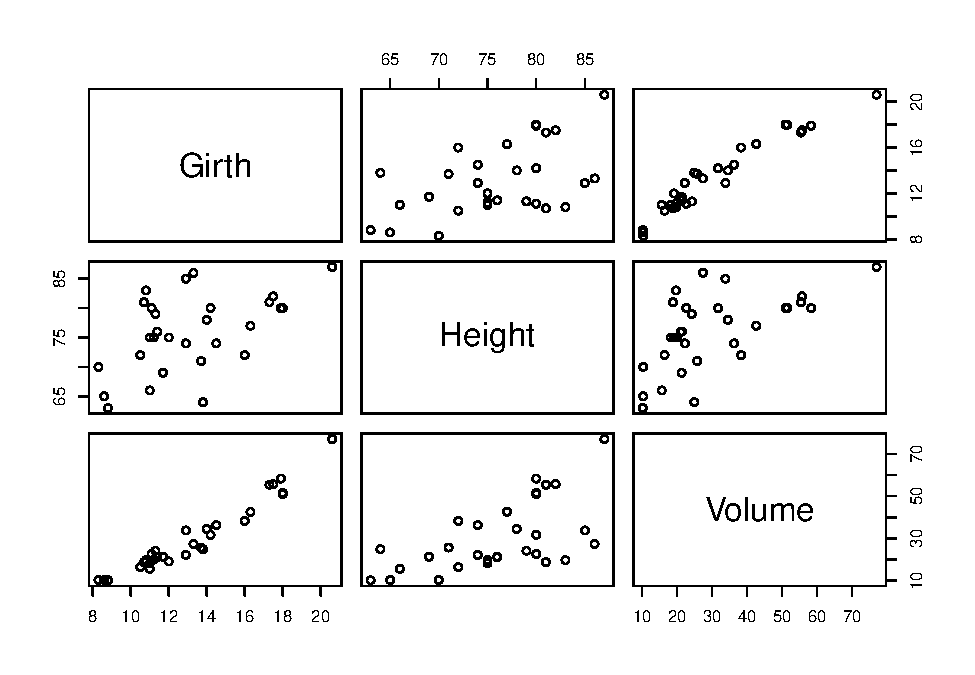
\includegraphics[width=0.9\linewidth]{Metode_Numerik_files/figure-latex/trees, LUfig-1} 

}

\caption{Scatterplot matriks dataset trees}(\#fig:trees, LUfig)
\end{figure}

Kita ingin membuat sebuah model linier untuk memprediksi \texttt{Volume} kayu berdasarkan variabel \texttt{Girth} dan \texttt{Heiht} atau volume sebagia fungsi dari variabel \texttt{Girth} dan \texttt{Heiht}. Kita dapat menuliskan relasi antara variabel volume sebagai fungsi dari variabel \texttt{Girth} dan \texttt{Heiht} menggunakan Persamaan \eqref{eq:trees}.

\begin{equation}
Volume=\beta_{girth} Girth+\beta_{height}Height+\beta_0
 \label{eq:trees}
\end{equation}

dimana \(\beta_0\) merupakan intersep persamaan regresi linier dan nilai \(\beta\) lainnya merupakan koefisien dari variabel \texttt{Girth} dan \texttt{Heiht}. Variabel \texttt{Volume} disebut sebagai variabel respon, sedangkan variabel \texttt{Girth} dan \texttt{Heiht} disebut sebagai variabel prediktor.

Metode kuadrat terkecil berusaha memperoleh seluruh koefisien variabel dan intersep dari persamaan regresi linier. Berdasarkan yang telah penulis jelaskan garis regresi terbaik adalah garis yang memiliki nilai kuadrat terkecil jarak antara titik observasi dan garis regresi. Dasar dari metode kuadrat terkecil merupakan persamaan yang relatif sederhana yang ditunjukkan pada Persamaan \eqref{eq:trees2}.

\begin{equation}
A^{T}A=A^{T}b
 \label{eq:trees2}
\end{equation}

dimana \(b\) merupakan vektor dari variabel respon (\texttt{Volume}) dan matrik \(A\) merupakan matriks variabel prediktor (variabel \texttt{Girth} dan \texttt{Heiht}).

Untuk menginputkan intercept kedalam persamaan linier kita perlu menmabhakan satu kolom di awal matriks \(A\) yang berisi nilai 1. Berikut adalah sintaks yang digunakan untuk membentuk matriks \(A\):

\begin{Shaded}
\begin{Highlighting}[]
\CommentTok{\# membentuk matriks A}
\NormalTok{pred }\OtherTok{\textless{}{-}} \FunctionTok{cbind}\NormalTok{(}\AttributeTok{intercept=}\DecValTok{1}\NormalTok{, }\AttributeTok{Girth=}\NormalTok{trees}\SpecialCharTok{$}\NormalTok{Girth, }\AttributeTok{Height=}\NormalTok{trees}\SpecialCharTok{$}\NormalTok{Height)}
\FunctionTok{head}\NormalTok{(A)}
\end{Highlighting}
\end{Shaded}

\begin{verbatim}
##      [,1] [,2] [,3]
## [1,]   27    6   -1
## [2,]    6   15    2
## [3,]    1    1   54
\end{verbatim}

Langkah selanjutnya adalah membentuk matriks \(b\). Berikut adalah sintaks yang digunakan:

\begin{Shaded}
\begin{Highlighting}[]
\NormalTok{resp}\OtherTok{\textless{}{-}}\NormalTok{ trees}\SpecialCharTok{$}\NormalTok{Volume}
\FunctionTok{head}\NormalTok{(resp)}
\end{Highlighting}
\end{Shaded}

\begin{verbatim}
## [1] 10.3 10.3 10.2 16.4 18.8 19.7
\end{verbatim}

Untuk memperoleh koefisien \(\beta\), kita dapat mencarinya dengan cara menyelesaikan Persamaan \eqref{eq:trees2}. Berikut adalah sintaks yang digunakan:

\begin{Shaded}
\begin{Highlighting}[]
\NormalTok{A }\OtherTok{\textless{}{-}} \FunctionTok{t}\NormalTok{(pred) }\SpecialCharTok{\%*\%}\NormalTok{ pred}
\NormalTok{b }\OtherTok{\textless{}{-}} \FunctionTok{t}\NormalTok{(pred) }\SpecialCharTok{\%*\%}\NormalTok{ resp}

\NormalTok{Ab }\OtherTok{\textless{}{-}} \FunctionTok{cbind}\NormalTok{(A,b)}
\NormalTok{(x }\OtherTok{\textless{}{-}} \FunctionTok{gauss\_jordan}\NormalTok{(Ab))}
\end{Highlighting}
\end{Shaded}

\begin{verbatim}
##           intercept Girth Height         
## intercept         1     0      0 -57.9877
## Girth             0     1      0   4.7082
## Height            0     0      1   0.3393
\end{verbatim}

Berdasarkan hasil yang diperoleh, persamaan linier yang terbentuk disajikan pada Persamaan \eqref{eq:trees3}.

\begin{equation}
Volume=4.7081605 Girth + 0.3392512 Height  -57.9876589
 \label{eq:trees3}
\end{equation}

Pembaca juga dapat menggunakan fungsi lain untuk memperoleh nilai koefisien tersebut, seperti: \texttt{lu\_solve()}dan\texttt{solve()}. untuk fungsi \texttt{jacobi()} dan \texttt{gauss\_seidel()}, kita harus pastikan syarat-syarat terkait metode tersebut. Berikut adalah contoh penyelesaian menggunakan sintaks lainnya:

\begin{Shaded}
\begin{Highlighting}[]
\CommentTok{\# metode LU}
\FunctionTok{lu\_solve}\NormalTok{(A,b)}
\end{Highlighting}
\end{Shaded}

\begin{verbatim}
## $P
##      [,1] [,2] [,3]
## [1,]    1    0    0
## [2,]    0    1    0
## [3,]    0    0    1
## 
## $L
##       [,1]  [,2] [,3]
## [1,]  1.00 0.000    0
## [2,] 13.25 1.000    0
## [3,] 76.00 1.054    1
## 
## $U
##           intercept Girth Height
## intercept        31 410.7 2356.0
## Girth             0 295.4  311.5
## Height            0   0.0  889.6
## 
## $result
##          [,1]
## [1,] -57.9877
## [2,]   4.7082
## [3,]   0.3393
\end{verbatim}

\begin{Shaded}
\begin{Highlighting}[]
\CommentTok{\# fungsi solve()}
\FunctionTok{solve}\NormalTok{(A,b)}
\end{Highlighting}
\end{Shaded}

\begin{verbatim}
##               [,1]
## intercept -57.9877
## Girth       4.7082
## Height      0.3393
\end{verbatim}

\texttt{R} juga menyediakan fungsi untuk membentuk model regresi linier. Fungsi yang digunakan adalah \texttt{lm()}. Berikut sintaks yang digunakan untuk membentuk model linier menggunakan fungsi \texttt{lm()}:

\begin{Shaded}
\begin{Highlighting}[]
\FunctionTok{lm}\NormalTok{(Volume}\SpecialCharTok{\textasciitilde{}}\NormalTok{Girth}\SpecialCharTok{+}\NormalTok{Height, }\AttributeTok{data=}\NormalTok{trees)}
\end{Highlighting}
\end{Shaded}

\begin{verbatim}
## 
## Call:
## lm(formula = Volume ~ Girth + Height, data = trees)
## 
## Coefficients:
## (Intercept)        Girth       Height  
##     -57.988        4.708        0.339
\end{verbatim}

\hypertarget{reaktorkimia}{%
\subsection{Aliran Massa Dalam Reaktor}\label{reaktorkimia}}

Pada \emph{sub-chapter} ini penulis akan memberikan penerapan aljabar linier untuk menghitung konsentrasi suatu zat atau parameter lingkungan dalam reaktor yang saling terhubung. Pada contoh kasus kali ini diasumsikan terdapat lima buah reaktor yang saling terhubung satu sama lain sesuai Gambar \ref{fig:reaktor}. Debit air (\(\frac{m^{3}}{detik}\)) dan konsentrasi zat pencemar (\(\frac{mg}{m^3}\)) disajikan pula diagram alir tersebut. Diasumsikan kelima buah reaktor tersebut dalam kondisi \emph{steady} dan volume reaktor diasumsikan sama. Kesetimbangan massa persatuan waktu dalam kondisi \emph{steady} disajikan pada Persamaan \eqref{eq:steady}.

\begin{figure}

{\centering 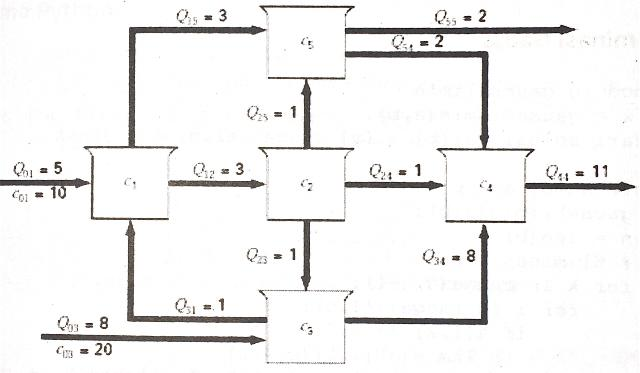
\includegraphics[width=0.9\linewidth]{./images/reaktor} 

}

\caption{Aliran massa dalam reaktor.}\label{fig:reaktor}
\end{figure}

\begin{equation}
m_in=m_out
 \label{eq:steady}
\end{equation}

\begin{equation}
Q_{in}C_{in}= Q_{out}C_{out}
 \label{eq:steady2}
\end{equation}

Berdasarkan Gambar \ref{fig:reaktor}, dapat dibentuk lima buah sistem persamaan linier. Persamaan linier yang terbentuk disajikan sebagai berikut:

\[
\begin{matrix}
  6c_{1}-c_{3}=50 \\
  -3c_{1}+3c_{2}=0 \\
  -c_{2}+9c_{3}=160 \\
  -c_{2}-8c_{3}+11c_{4}-2c_{5}=0 \\
  -3c_{1}-c_{2}+4c_{5}=0
\end{matrix}
\]

Untuk menyelesaiakan sistem persamaan linier tersebut dan memperoleh nilai \(c\) dari masing-masing reaktor, kiat perlu mengubahnya dulu kedalam bentuk matriks \(Ax=b\). Berikut adalah matriks yang terbentuk:

\begin{equation*}
\begin{bmatrix}
      6 &  0 & -1 & 0  & 0    \\[0.3em]
     -3 &  3 & 0  & 0  & 0    \\[0.3em]
      0 & -1 & 9  & 0  & 0    \\[0.3em]
      0 & -1 & -8 & 11 & -2   \\[0.3em]
     -3 & -1 & 0  & 0  & 4
\end{bmatrix}
c = \begin{bmatrix}
     50     \\[0.3em]
     0      \\[0.3em]
     160    \\[0.3em]
     0      \\[0.3em]
     0
\end{bmatrix}
\end{equation*}

Kita akan menyelesaikannya dengan menggunakan metode elminasi Gauss-Jordan, dekomposisi LU, iterasi Jacobi, dan iterasi Gauss-Seidel. Untuk dapat menyelesaikannya menggunakan metode-metode tersebut pada \texttt{R}, kita perlu membentuk matriksnya terlebih dahulu:

\begin{Shaded}
\begin{Highlighting}[]
\NormalTok{(A }\OtherTok{\textless{}{-}} \FunctionTok{matrix}\NormalTok{(}\FunctionTok{c}\NormalTok{(}\DecValTok{6}\NormalTok{,}\SpecialCharTok{{-}}\DecValTok{3}\NormalTok{,}\DecValTok{0}\NormalTok{,}\DecValTok{0}\NormalTok{,}\SpecialCharTok{{-}}\DecValTok{3}\NormalTok{,}
              \DecValTok{0}\NormalTok{,}\DecValTok{3}\NormalTok{,}\SpecialCharTok{{-}}\DecValTok{1}\NormalTok{,}\SpecialCharTok{{-}}\DecValTok{1}\NormalTok{,}\SpecialCharTok{{-}}\DecValTok{1}\NormalTok{,}
              \SpecialCharTok{{-}}\DecValTok{1}\NormalTok{,}\DecValTok{0}\NormalTok{,}\DecValTok{9}\NormalTok{,}\SpecialCharTok{{-}}\DecValTok{8}\NormalTok{,}\DecValTok{0}\NormalTok{,}
              \DecValTok{0}\NormalTok{,}\DecValTok{0}\NormalTok{,}\DecValTok{0}\NormalTok{,}\DecValTok{11}\NormalTok{,}\DecValTok{0}\NormalTok{,}
              \DecValTok{0}\NormalTok{,}\DecValTok{0}\NormalTok{,}\DecValTok{0}\NormalTok{,}\SpecialCharTok{{-}}\DecValTok{2}\NormalTok{,}\DecValTok{4}\NormalTok{),}\AttributeTok{nrow=}\DecValTok{5}\NormalTok{))}
\end{Highlighting}
\end{Shaded}

\begin{verbatim}
##      [,1] [,2] [,3] [,4] [,5]
## [1,]    6    0   -1    0    0
## [2,]   -3    3    0    0    0
## [3,]    0   -1    9    0    0
## [4,]    0   -1   -8   11   -2
## [5,]   -3   -1    0    0    4
\end{verbatim}

\begin{Shaded}
\begin{Highlighting}[]
\NormalTok{(b }\OtherTok{\textless{}{-}} \FunctionTok{c}\NormalTok{(}\DecValTok{50}\NormalTok{,}\DecValTok{0}\NormalTok{,}\DecValTok{160}\NormalTok{,}\DecValTok{0}\NormalTok{,}\DecValTok{0}\NormalTok{))}
\end{Highlighting}
\end{Shaded}

\begin{verbatim}
## [1]  50   0 160   0   0
\end{verbatim}

\textbf{Metode Eliminasi Gauss-Jordan}

\begin{Shaded}
\begin{Highlighting}[]
\FunctionTok{gauss\_jordan}\NormalTok{(}\FunctionTok{cbind}\NormalTok{(A,b))}
\end{Highlighting}
\end{Shaded}

\begin{verbatim}
##                    b
## [1,] 1 0 0 0 0 11.51
## [2,] 0 1 0 0 0 11.51
## [3,] 0 0 1 0 0 19.06
## [4,] 0 0 0 1 0 17.00
## [5,] 0 0 0 0 1 11.51
\end{verbatim}

\textbf{Metode Dekomposisi LU}

\begin{Shaded}
\begin{Highlighting}[]
\FunctionTok{lu\_solve}\NormalTok{(A,b)}
\end{Highlighting}
\end{Shaded}

\begin{verbatim}
## $P
##      [,1] [,2] [,3] [,4] [,5]
## [1,]    1    0    0    0    0
## [2,]    0    1    0    0    0
## [3,]    0    0    1    0    0
## [4,]    0    0    0    1    0
## [5,]    0    0    0    0    1
## 
## $L
##      [,1]    [,2]     [,3] [,4] [,5]
## [1,]  1.0  0.0000  0.00000    0    0
## [2,] -0.5  1.0000  0.00000    0    0
## [3,]  0.0 -0.3333  1.00000    0    0
## [4,]  0.0 -0.3333 -0.92453    1    0
## [5,] -0.5 -0.3333 -0.07547    0    1
## 
## $U
##      [,1] [,2]       [,3] [,4] [,5]
## [1,]    6    0 -1.000e+00    0    0
## [2,]    0    3 -5.000e-01    0    0
## [3,]    0    0  8.833e+00    0    0
## [4,]    0    0  0.000e+00   11   -2
## [5,]    0    0  1.110e-16    0    4
## 
## $result
## [1] 11.51 11.51 19.06 17.00 11.51
\end{verbatim}

\textbf{Metode Iterasi Jacobi}

\begin{Shaded}
\begin{Highlighting}[]
\FunctionTok{jacobi}\NormalTok{(A,b, }\AttributeTok{maxiter=}\DecValTok{100}\NormalTok{)}
\end{Highlighting}
\end{Shaded}

\begin{verbatim}
## $X
##       [,1]
## [1,] 11.51
## [2,] 11.51
## [3,] 19.06
## [4,] 17.00
## [5,] 11.51
## 
## $iter
## [1] 17
\end{verbatim}

\textbf{Metode Iterasi Gauss-Seidel}

\begin{Shaded}
\begin{Highlighting}[]
\FunctionTok{gauss\_seidel}\NormalTok{(A,b, }\AttributeTok{maxiter=}\DecValTok{200}\NormalTok{)}
\end{Highlighting}
\end{Shaded}

\begin{verbatim}
## $X
##       [,1]
## [1,] 11.51
## [2,] 11.51
## [3,] 19.06
## [4,] 17.00
## [5,] 11.51
## 
## $iter
## [1] 7
\end{verbatim}

Berdasarkan seluruh metode tersebut, diperoleh konsentrasi zat pencemar pada masing-masing reaktor adalah sebagai berikut:

\[
\begin{matrix}
  c_{1}=11,50943 \frac{mg}{m^3} \\
  c_{2}=11,50943 \frac{mg}{m^3} \\
  c_{3}=19,05660 \frac{mg}{m^3} \\
  c_{4}=16,99828 \frac{mg}{m^3} \\
  c_{5}=11.50943 \frac{mg}{m^3}
\end{matrix}
\]

\hypertarget{referensi-5}{%
\section{Referensi}\label{referensi-5}}

\begin{enumerate}
\def\labelenumi{\arabic{enumi}.}
\tightlist
\item
  Bloomfield, V.A. 2014. \textbf{Using R for Numerical Analysis in Science and Engineering}. CRC Press
\item
  Howard, J.P. 2017. \textbf{Computational Methods for Numerical Analysis with R}. CRC Press.
\item
  Kreyszig, E. 2011. \textbf{Advanced Engineering Mathematics, 10th Edition}. John Wiley \& Sons.
\item
  Primartha, R. 2018. \textbf{Belajar Machine Learning Teori dan Praktik}. Penerbit Informatika : Bandung.
\item
  Sanjaya, M. 2015. \textbf{Metode Numerik Berbasis Phython}. Penerbit Gava Media: Yogyakarta.
\item
  Suparno, S. 2008. \textbf{Komputasi untuk Sains dan Teknik Edisi II}. Departemen Fisika-FMIPA Universitas Indonesia.
\end{enumerate}

\hypertarget{latihan}{%
\section{Latihan}\label{latihan}}

\begin{enumerate}
\def\labelenumi{\arabic{enumi}.}
\tightlist
\item
  Selesaikan sistem persamaan linier berikut menggunakan eliminasi Gauss!
\end{enumerate}

\[
\begin{matrix}
  -4x+4y=-1 \\
  -2x+2y-3z=-3 \\
  3x+1y-3z=-3
\end{matrix}
\]

\begin{enumerate}
\def\labelenumi{\arabic{enumi}.}
\setcounter{enumi}{1}
\tightlist
\item
  Carilah penyelesaian dari sistem persamaan linier soal no.1 menggunakan algoritma dekomposisi LU!
\item
  Tunjukan 5 iterasi pertama sistem persamaan linier berikut menggunakan algoritma Jacobi dan Gauss-Seidel!
\end{enumerate}

\[
\begin{matrix}
  3x+2y-1z=-3 \\
  -3x-3y-3z=9 \\
  1y-1z=-1
\end{matrix}
\]

\begin{enumerate}
\def\labelenumi{\arabic{enumi}.}
\setcounter{enumi}{3}
\tightlist
\item
  Gunakan fungsi \texttt{jacobi()} dan \texttt{gauss\_seidel()} untuk menyelesaikan sistem persamaan linier pada soal no.4 dan tentukan metode mana yang paling cepat memperoleh penyelesaian? (\textbf{petunjuk}: gunakan fungsi \texttt{system.time()} dan jumlah iterasi yang diperlukan untuk memperoleh hasil yang konvergen)
\item
  Apakah yang terjadi jika kita menginputkan matriks segiempat \(A\) kedalam fungsi \texttt{solve()} dan apa yang akan terjadi jika selanjutnya argumen pada fungsi tersebut juga menyertakan vektor \(b\)?
\item
  Dengan menggunakan dataset \texttt{mtcars} buatlah persamaan linier variabel \texttt{mpg} sebagai fungsi dari variabel \texttt{wt}, \texttt{hp}, dan \texttt{qsec} menggunakan algoritma dekomposisi LU?
\end{enumerate}

\hypertarget{rootfinding}{%
\chapter{Akar Persamaan Non-Linier}\label{rootfinding}}

Persamaan non-linier dapat diartikan sebagai persamaan yang tidak mengandung syarat seperti persamaan linier, sehingga persamaan non-linier dapat merupakan:

\begin{enumerate}
\def\labelenumi{\alph{enumi}.}
\tightlist
\item
  Persamaan yang memiliki pangkat selain satu (misal: \(x^2\))
\item
  Persamaan yang mempunyai produk dua variabel (misal: \(xy\))
\end{enumerate}

Dalam penyelesaian persamaan non-linier diperlukan akar-akar persamaan non-linier, dimana akar sebuah persamaan non-linier \(f\left(x\right)=0\) merupakan nilai \(x\) yang menyebabkan nilai \(f\left(x\right)\) sama dengan nol. Dalam hal ini dapat disimpulkan bahwa akar-akar penyelesaian persamaan non-linier merupakan titik potong antara kurva \(f\left(x\right)\) dengan sumbu \(x\). Ilustrasi penjelasan tersebut ditampilkan pada Gambar \ref{fig:root}.

\begin{figure}

{\centering 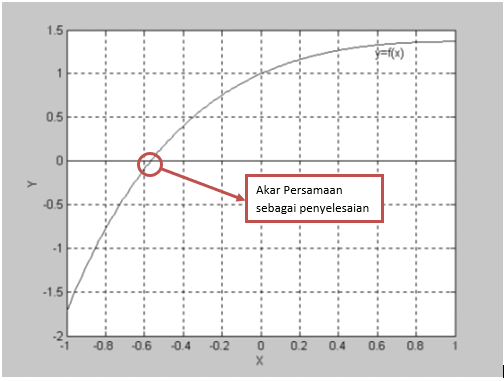
\includegraphics[width=0.8\linewidth]{./images/root} 

}

\caption{Penyelesaian persamaan non-linier.}\label{fig:root}
\end{figure}

Contoh sederhana dari penentuan akar persamaan non-linier adalah penentuan akar persamaan kuadratik. Secara analitik penentuan akar persamaan kuadratik dapat dilakukan menggunakan Persamaan \eqref{eq:kuadratik}.

\begin{equation}
x_{1,2}=\frac{-b\pm\sqrt{b^2-4a}}{2a}
  \label{eq:kuadratik}
\end{equation}

Untuk masalah yang lebih rumit, penyelesaian analitik sudah tidak mungkin dilakukan. Metode numerik dapat digunakan untuk menyelesaikan masalah yang lebih kompleks. Untuk mengetahui apakah suatu persamaan non-linier memiliki akar-akar penyelesaian atau tidak, diperlukan analisa menggunakan Teorema berikut:

\begin{theorem}[root]
\protect\hypertarget{thm:unnamed-chunk-206}{}\label{thm:unnamed-chunk-206}Suatu range x={[}a,b{]} mempunyai akar bila f(a) dan f(b) berlawanan tanda atau memenuhi f(a).f(b)\textless0
\end{theorem}

Untuk memahami teorema tersebut perhatikan ilustrasi pada Gambar \ref{fig:Bolzano}.

\begin{figure}

{\centering \includegraphics[width=0.8\linewidth]{./images/Bolzano} 

}

\caption{Ilustrasi teorema Bolzano.}\label{fig:Bolzano}
\end{figure}

Pada Chapter \ref{rootfinding} ini, akan dilakukan sejumlah pembahasan antara lain:

\begin{itemize}
\tightlist
\item
  penentuan akar persamaan dengan metode tertutup
\item
  penentuan akar persamaan dengan metode terbuka
\item
  fungsi-fungsi \texttt{R} untuk mementukan akar persamaan non-linier
\item
  studi kasus
\end{itemize}

\hypertarget{bracketing}{%
\section{Metode Tertutup}\label{bracketing}}

Metode tertutup disebut juga metode \emph{bracketing}. Disebut sebagai metode tertutup karena dalam pencarian akar-akar persamaan non-linier dilakukan dalam suatu selang \(\left[a,b \right]\).

\hypertarget{table}{%
\subsection{Metode Tabel}\label{table}}

Penyelesaian persamaan non-linier menggunakan metode tabel dilakukan dengan membagi persamaan menjadi beberapa area, dimana untuk \(x=\left[a,b \right]\) dibagi sebanyak \(N\) bagian dan pada masing-masing bagian dihitung nilai \(f\left(x \right)\) sehingga diperoleh nilai \(f\left(x \right)\) pada setian \(N\) bagian.

Bila nilai \(f\left(x_k \right)=0\) atau mendekati nol, dimana \(a \le k \le b\), maka dikatakan bahwa \(x_k\) adalah penyelesaian persamaan \(f\left(x \right)\). Bila tidak ditemukan, dicari nilai \(f\left(x_k \right)\) dan \(f\left(x_{k+1} \right)\) yang berlawanan tanda. Bila tidak ditemukan, maka persamaan tersebut dapat dikatakan tidak mempunyai akar untuk rentang \(\left[a,b \right]\).

Bila akar persamaan tidak ditemukan, maka ada dua kemungkinan untuk menentukan akar persamaan, yaitu:

\begin{enumerate}
\def\labelenumi{\alph{enumi}.}
\tightlist
\item
  Akar persamaan ditentukan oleh nilai mana yang lebih dekat. Bila \(f\left(x_k\right)\le f\left(x_{k+1}\right)\), maka akarnya \(x_k\). Bila \(f\left(x_{k+1}\right)\le f\left(x_{k}\right)\), maka akarnya \(x_{k+1}\).
\item
  Perlu dicari lagi menggunakan rentang \(x=\left[x_{k}, x_{k+1} \right]\).
\end{enumerate}

Secara grafis penyelesaian persamaan non-linier menggunakan metode table disajikan pada Gambar \ref{fig:tabelviz}.

\begin{figure}

{\centering \includegraphics[width=0.8\linewidth]{./images/tabelviz} 

}

\caption{Ilustrasi metode tabel.}\label{fig:tabelviz}
\end{figure}

\begin{center}\rule{0.5\linewidth}{0.5pt}\end{center}

\textbf{Algoritma Metode Tabel}

\begin{enumerate}
\def\labelenumi{\arabic{enumi}.}
\tightlist
\item
  Definisikan fungsi \(f\left(x \right)\)
\item
  Tentukan rentang untuk \(x\) yang berupa batas bawah \(a\) dan batas atas \(b\).
\item
  Tentukan jumlah pembagi \(N\)
\item
  Hitung step pembagi
\end{enumerate}

\begin{equation}
h=\frac{b+a}{N}
  \label{eq:tabel1}
\end{equation}

\begin{enumerate}
\def\labelenumi{\arabic{enumi}.}
\setcounter{enumi}{4}
\tightlist
\item
  Untuk \(i=0\) s/d \(N\), hitung:
\end{enumerate}

\begin{equation}
x_i=a+i.h
  \label{eq:tabel2}
\end{equation}

\begin{equation}
y_i=f\left(x_i \right)
  \label{eq:tabel3}
\end{equation}

\begin{enumerate}
\def\labelenumi{\arabic{enumi}.}
\setcounter{enumi}{5}
\tightlist
\item
  Untuk \(i=0\) s/d \(N\), dimana
\end{enumerate}

\begin{itemize}
\item
  Bila \(f\left(x \right)=0\), maka akarnya \(x_k\)
\item
  Bila \(f\left(a \right) f\left(b \right) <0\), maka:

  \begin{itemize}
  \tightlist
  \item
    \(f\left(x_k\right)\le f\left(x_{k+1}\right)\), maka akarnya \(x_k\)
  \item
    Bila tida, \(x_{k+1}\) adalah penyelesaian atau dapat dikatakan penyelesaian berada diantara \(x_k\) dan \(x_{k+1}\).
  \end{itemize}
\end{itemize}

\begin{center}\rule{0.5\linewidth}{0.5pt}\end{center}

Kita dapat membuat suatu fungsi pada \texttt{R} untuk melakukan proses iterasi pada metode Tabel. Fungsi \texttt{root\_table()} akan melakukan iterasi berdasarkan step algoritma 1 sampai 5. Berikut adalah sintaks yang digunakan:

\begin{Shaded}
\begin{Highlighting}[]
\NormalTok{root\_table }\OtherTok{\textless{}{-}} \ControlFlowTok{function}\NormalTok{(f, a, b, }\AttributeTok{N=}\DecValTok{20}\NormalTok{)\{}
\NormalTok{    h }\OtherTok{\textless{}{-}} \FunctionTok{abs}\NormalTok{((a}\SpecialCharTok{+}\NormalTok{b)}\SpecialCharTok{/}\NormalTok{N)}
\NormalTok{    x }\OtherTok{\textless{}{-}} \FunctionTok{seq}\NormalTok{(}\AttributeTok{from=}\NormalTok{a, }\AttributeTok{to=}\NormalTok{b, }\AttributeTok{by=}\NormalTok{h)}
\NormalTok{    fx }\OtherTok{\textless{}{-}} \FunctionTok{rep}\NormalTok{(}\DecValTok{0}\NormalTok{, N}\SpecialCharTok{+}\DecValTok{1}\NormalTok{)}
    \ControlFlowTok{for}\NormalTok{(i }\ControlFlowTok{in} \DecValTok{1}\SpecialCharTok{:}\NormalTok{(N}\SpecialCharTok{+}\DecValTok{1}\NormalTok{))\{}
\NormalTok{      fx[i] }\OtherTok{\textless{}{-}} \FunctionTok{f}\NormalTok{(x[i])}
\NormalTok{    \}}
\NormalTok{    data }\OtherTok{\textless{}{-}} \FunctionTok{data.frame}\NormalTok{(}\AttributeTok{x=}\NormalTok{x, }\AttributeTok{fx=}\NormalTok{fx)}
    \FunctionTok{return}\NormalTok{(data)}
\NormalTok{\}}
\end{Highlighting}
\end{Shaded}

\begin{example}
\protect\hypertarget{exm:tabelexmp}{}\label{exm:tabelexmp}Carilah akar persamaan \(f\left(x \right)=x+e^{x}\) pada rentang \(x=\left[-1,0 \right]\)?
\end{example}

\textbf{Jawab}:

Sebagai permulaan, jumlah pembagi yang digunakan adalah \(N=10\). Dengan menggunakan fungsi \texttt{root\_table()} diperoleh hasil yang disajikan pada Tabel \ref{tab:tabeltabel}.

\begin{Shaded}
\begin{Highlighting}[]
\NormalTok{tabel }\OtherTok{\textless{}{-}} \FunctionTok{root\_table}\NormalTok{(}\AttributeTok{f=}\ControlFlowTok{function}\NormalTok{(x)\{x}\SpecialCharTok{+}\FunctionTok{exp}\NormalTok{(x)\},}
                     \AttributeTok{a=}\SpecialCharTok{{-}}\DecValTok{1}\NormalTok{, }\AttributeTok{b=}\DecValTok{0}\NormalTok{, }\AttributeTok{N=}\DecValTok{10}\NormalTok{)}
\end{Highlighting}
\end{Shaded}

\begin{table}

\caption{\label{tab:tabeltabel}Penyelesaian persamaan x+exp(x)=0}
\centering
\begin{tabular}[t]{r|r}
\hline
x & fx\\
\hline
-1.0 & -0.6321\\
\hline
-0.9 & -0.4934\\
\hline
-0.8 & -0.3507\\
\hline
-0.7 & -0.2034\\
\hline
-0.6 & -0.0512\\
\hline
-0.5 & 0.1065\\
\hline
-0.4 & 0.2703\\
\hline
-0.3 & 0.4408\\
\hline
-0.2 & 0.6187\\
\hline
-0.1 & 0.8048\\
\hline
0.0 & 1.0000\\
\hline
\end{tabular}
\end{table}

Berdasarkan Tabel \ref{tab:tabeltabel} diperoleh penyelesaian di antara \(-0,6\) dan \(-0,5\) dengan nilai \(f\left(x \right)\) masing-masing sebesar \(-0,0512\) dan \(-0,1065\), sehingga dapat diambil penyelesaian \(x=-0,6\). Kita dapat terus melakukan iterasi sampai memperoleh nilai \(f\left(x \right)\) \textless{} nilai toleransi dengan terus merubah rentang yang diberikan. Iterasi berikutnya dengan nilai pembagi sama dan rentang nilai \(x=\left[-0,6;-0,5\right]\) diperoleh nilai \(x=-0,57\) dan \(f\left(x \right)=0,00447\).

Untuk melihat gambaran lokasi akar, kita dapat pulang mengeplotkan data menggunakan fungsi plot. Berikut adalah fungsi yang digunakan:

\begin{figure}

{\centering \includegraphics[width=0.8\linewidth]{Metode_Numerik_files/figure-latex/tabelplot-1} 

}

\caption{Plot fungsi x+exp(x) pada rentang -1 sampai 0.}\label{fig:tabelplot}
\end{figure}

Untuk mengetahui lokasi akar dengan lebih jelas, kita dapat memperkecil lagi rentang nilai yang dimasukkan dalam fungsi \texttt{curve()}.

Metode tabel pada dasarnya memiliki kelemahan yaitu cukup sulit untuk memdapatkan error penyelesaian yang cukup kecil, sehingga metode ini jarang sekali digunakan untuk menyelesaikan persamaan non-linier. Namun, metode ini cukup baik digunakan dalam menentukan area penyelesaian sehingga dapat dijadikan acuan metode lain yang lebih baik.

\hypertarget{bisection}{%
\subsection{Metode Biseksi}\label{bisection}}

Prinsip metode bagi dua adalah mengurung akar fungsi pada interval \(x=\left[a,b \right]\) atau pada nilai \(x\) batas bawah \(a\) dan batas atas \(b\). Selanjutnya interval tersebut terus menerus dibagi 2 hingga sekecil mungkin, sehingga nilai hampiran yang dicari dapat ditentukan dengan tingkat toleransi tertentu. Untuk lebih memahami metode biseksi, perhatikan visualisasi pada Gambar \ref{fig:biseksi}.

\begin{figure}

{\centering \includegraphics[width=0.8\linewidth]{./images/biseksi} 

}

\caption{Ilustrasi metode biseksi.}\label{fig:biseksi}
\end{figure}

Metode biseksi merupakan metode yang paling mudah dan paling sederhana dibanding metode lainnya. Adapun sifat metode ini antara lain:

\begin{enumerate}
\def\labelenumi{\arabic{enumi}.}
\tightlist
\item
  Konvergensi lambat
\item
  Caranya mudah
\item
  Tidak dapat digunakan untuk mencari akar imaginer
\item
  Hanya dapat mencari satu akar pada satu siklus.
\end{enumerate}

\begin{center}\rule{0.5\linewidth}{0.5pt}\end{center}

\textbf{Algoritma Metode Biseksi}

\begin{enumerate}
\def\labelenumi{\arabic{enumi}.}
\tightlist
\item
  Definisikan fungsi \(f\left(x \right)\)
\item
  Tentukan rentang untuk \(x\) yang berupa batas bawah \(a\) dan batas atas \(b\).
\item
  Tentukan nilai toleransi \(e\) dan iterasi maksimum \(N\)
\item
  Hitung \(f\left(a \right)\) dan \(f\left(b \right)\)
\item
  Hitung:
\end{enumerate}

\begin{equation}
x=\frac{a+b}{2}
  \label{eq:biseksi1}
\end{equation}

\begin{enumerate}
\def\labelenumi{\arabic{enumi}.}
\setcounter{enumi}{5}
\tightlist
\item
  Hitung \(f\left(x \right)\)
\item
  Bila \(f\left(x \right).f\left(a \right)<0\), maka \(b=x\) dan \(f\left(b \right)=f\left(x \right)\). Bila tidak, \(a=x\) dan \(f\left(a \right)=f\left(x \right)\)
\item
  Bila \(\left|b-a \right|<e\) atau iterasi maksimum maka proses dihentikan dan didapatkan akar=\(x\), dan bila tidak ulangi langkah 6.
\item
  Jika sudah diperoleh nilai dibawah nilai toleransi, nilai akar selanjutnya dihitung berdasarkan Persamaan \eqref{eq:biseksi1} dengan nilai \(a\) dan \(b\) merupakan nilai baru yang diperoleh dari proses iterasi.
\end{enumerate}

\begin{center}\rule{0.5\linewidth}{0.5pt}\end{center}

Berdasarkan algoritma tersebut, kita dapat menyusun suatu fungsi pada \texttt{R} yang dapat digunakan untuk melakukan iterasi tersebut. Fungsi \texttt{root\_bisection()} merupakan fungsi yang telah penulis susun untuk melakukan iterasi menggunakan metode biseksi. Berikut adalah sintaks dari fungsi tersebut:

\begin{Shaded}
\begin{Highlighting}[]
\NormalTok{root\_bisection }\OtherTok{\textless{}{-}} \ControlFlowTok{function}\NormalTok{(f, a, b, }\AttributeTok{tol=}\FloatTok{1e{-}7}\NormalTok{, }\AttributeTok{N=}\DecValTok{100}\NormalTok{)\{}
\NormalTok{  iter }\OtherTok{\textless{}{-}} \DecValTok{0}
\NormalTok{  fa }\OtherTok{\textless{}{-}} \FunctionTok{f}\NormalTok{(a)}
\NormalTok{  fb }\OtherTok{\textless{}{-}} \FunctionTok{f}\NormalTok{(b)}
  
  \ControlFlowTok{while}\NormalTok{(}\FunctionTok{abs}\NormalTok{(b}\SpecialCharTok{{-}}\NormalTok{a)}\SpecialCharTok{\textgreater{}}\NormalTok{tol)\{}
\NormalTok{    iter }\OtherTok{\textless{}{-}}\NormalTok{ iter}\SpecialCharTok{+}\DecValTok{1}
    \ControlFlowTok{if}\NormalTok{(iter}\SpecialCharTok{\textgreater{}}\NormalTok{N)\{}
      \FunctionTok{warning}\NormalTok{(}\StringTok{"iterations maximum exceeded"}\NormalTok{)}
      \ControlFlowTok{break}
\NormalTok{    \}}
\NormalTok{    x }\OtherTok{\textless{}{-}}\NormalTok{ (a}\SpecialCharTok{+}\NormalTok{b)}\SpecialCharTok{/}\DecValTok{2}
\NormalTok{    fx }\OtherTok{\textless{}{-}} \FunctionTok{f}\NormalTok{(x)}
    \ControlFlowTok{if}\NormalTok{(fa}\SpecialCharTok{*}\NormalTok{fx}\SpecialCharTok{\textgreater{}}\DecValTok{0}\NormalTok{)\{}
\NormalTok{      a }\OtherTok{\textless{}{-}}\NormalTok{ x}
\NormalTok{      fa }\OtherTok{\textless{}{-}}\NormalTok{ fx}
\NormalTok{    \} }\ControlFlowTok{else}\NormalTok{\{}
\NormalTok{      b }\OtherTok{\textless{}{-}}\NormalTok{ x}
\NormalTok{      fb }\OtherTok{\textless{}{-}}\NormalTok{ fx}
\NormalTok{    \}}
\NormalTok{  \}}
  
  \CommentTok{\# iterasi nilai x sebagai return value}
\NormalTok{  root }\OtherTok{\textless{}{-}}\NormalTok{ (a}\SpecialCharTok{+}\NormalTok{b)}\SpecialCharTok{/}\DecValTok{2}
  \FunctionTok{return}\NormalTok{(}\FunctionTok{list}\NormalTok{(}\StringTok{\textasciigrave{}}\AttributeTok{function}\StringTok{\textasciigrave{}}\OtherTok{=}\NormalTok{f, }\AttributeTok{root=}\NormalTok{root, }\AttributeTok{iter=}\NormalTok{iter))}
\NormalTok{\}}
\end{Highlighting}
\end{Shaded}

\begin{example}
\protect\hypertarget{exm:biseksexmp}{}\label{exm:biseksexmp}Carilah akar persamaan \(f\left(x \right)=xe^{-x}+1\) pada rentang \(x=\left[-1,0 \right]\) dengan nilai toleransi sebesar \(10^-7\)?
\end{example}

\textbf{Jawab}:

Langkah pertama dalam penghitungan adalah menghitung nilai \(x\) menggunakan Persamaan \eqref{eq:biseksi1}.

\[
x=\frac{-1+0}{2}=-0,5
\]

Hitung nilai \(f\left(x \right)\) dan \(f\left(a \right)\).

\[
f\left(x \right)=-0,5.e^{0,5}+1=0,175639
\]

\[
f\left(a \right)=-1.e^{1}+1=-1,71828
\]

Berdasarkan hasil perhitungan diperoleh:

\[
f\left(x \right).f\left(a \right)<0
\]

Sehingga \(b=x\) dan \(f\left(b \right)=f\left(x \right)\). Iterasi dilakukan kembali dengan menggunakan nilai \(b\) tersebut.

Untuk mempersingkat waktu iterasi kita akan menggunakan fungsi \texttt{root\_bisection()} pada \texttt{R}. Berikut adalah sintaks yang digunakan:

\begin{Shaded}
\begin{Highlighting}[]
\FunctionTok{root\_bisection}\NormalTok{(}\ControlFlowTok{function}\NormalTok{(x)\{x}\SpecialCharTok{*}\FunctionTok{exp}\NormalTok{(}\SpecialCharTok{{-}}\NormalTok{x)}\SpecialCharTok{+}\DecValTok{1}\NormalTok{\},}
               \AttributeTok{a=}\SpecialCharTok{{-}}\DecValTok{1}\NormalTok{, }\AttributeTok{b=}\DecValTok{0}\NormalTok{)}
\end{Highlighting}
\end{Shaded}

\begin{verbatim}
## $`function`
## function(x){x*exp(-x)+1}
## <bytecode: 0x000001ba8086f4b0>
## 
## $root
## [1] -0.5671
## 
## $iter
## [1] 24
\end{verbatim}

Berdasarkan hasil iterasi diperoleh akar persamaan \(x=-2.980232e-08\) dan iterasi yang diperlukan untuk memperolehnya sebanyak \(24\) iterasi.

\hypertarget{regulafalsi}{%
\subsection{Metode Regula Falsi}\label{regulafalsi}}

Metode regula falsi merupakan metode yang menyerupai metode biseksi, dimana iterasi dilakukan dengan terus melakukan pembaharuan rentang untuk memperoleh akar persamaan. Hal yang membedakan metode ini dengan metode biseksi adalah pencarian akar didasarkan pada slope (kemiringan) dan selisih tinggi dari kedua titik rentang. Titik pendekatan pada metode regula-falsi disajikan pada Persamaan \eqref{eq:rf}.

\begin{equation}
x=\frac{f\left(b\right).a-f\left(a\right).b}{f\left(b\right)-f\left(a\right)}
  \label{eq:rf}
\end{equation}

Ilustrasi dari metode regula falsi disajikan pada Gambar \ref{fig:regula}.

\begin{figure}

{\centering \includegraphics[width=0.8\linewidth]{./images/regula} 

}

\caption{Ilustrasi metode regula falsi.}\label{fig:regula}
\end{figure}

\begin{center}\rule{0.5\linewidth}{0.5pt}\end{center}

\textbf{Algoritma Metode Regula Falsi}

\begin{enumerate}
\def\labelenumi{\arabic{enumi}.}
\tightlist
\item
  Definisikan fungsi \(f\left(x \right)\)
\item
  Tentukan rentang untuk \(x\) yang berupa batas bawah \(a\) dan batas atas \(b\).
\item
  Tentukan nilai toleransi \(e\) dan iterasi maksimum \(N\)
\item
  Hitung \(f\left(a \right)\) dan \(f\left(b \right)\)
\item
  Untuk iterasi \(i=1\) s/d \(N\)
\end{enumerate}

\begin{itemize}
\tightlist
\item
  Hitung nilai \(x\) berdasarkan Persamaan \eqref{eq:rf}
\item
  Hitung \(f\left(x \right)\)
\item
  Hitung \(error=\left|f\left(x \right) \right|\)
\item
  Jika \(f\left(x \right).f\left(a \right)<0\), maka \(b=x\) dan \(f\left(b \right)=f\left(x \right)\). Jika tidak, \(a=x\) dan \(f\left(a \right)=f\left(x \right)\).
\end{itemize}

\begin{enumerate}
\def\labelenumi{\arabic{enumi}.}
\setcounter{enumi}{5}
\tightlist
\item
  Akar persamaan adalah \(x\)
\end{enumerate}

\begin{center}\rule{0.5\linewidth}{0.5pt}\end{center}

Fungsi \texttt{root\_rf()} didasarkan pada langkah-langkah di atas. Sintaks fungsi tersebut adalah sebagai berikut:

\begin{Shaded}
\begin{Highlighting}[]
\NormalTok{root\_rf }\OtherTok{\textless{}{-}} \ControlFlowTok{function}\NormalTok{(f, a, b, }\AttributeTok{tol=}\FloatTok{1e{-}7}\NormalTok{, }\AttributeTok{N=}\DecValTok{100}\NormalTok{)\{}
\NormalTok{  iter }\OtherTok{\textless{}{-}} \DecValTok{1}
\NormalTok{  fa }\OtherTok{\textless{}{-}} \FunctionTok{f}\NormalTok{(a)}
\NormalTok{  fb }\OtherTok{\textless{}{-}} \FunctionTok{f}\NormalTok{(b)}
\NormalTok{  x }\OtherTok{\textless{}{-}}\NormalTok{ ((fb}\SpecialCharTok{*}\NormalTok{a)}\SpecialCharTok{{-}}\NormalTok{(fa}\SpecialCharTok{*}\NormalTok{b))}\SpecialCharTok{/}\NormalTok{(fb}\SpecialCharTok{{-}}\NormalTok{fa)}
\NormalTok{  fx }\OtherTok{\textless{}{-}} \FunctionTok{f}\NormalTok{(x)}
  
  \ControlFlowTok{while}\NormalTok{(}\FunctionTok{abs}\NormalTok{(fx)}\SpecialCharTok{\textgreater{}}\NormalTok{tol)\{}
\NormalTok{    iter }\OtherTok{\textless{}{-}}\NormalTok{ iter}\SpecialCharTok{+}\DecValTok{1}
    \ControlFlowTok{if}\NormalTok{(iter}\SpecialCharTok{\textgreater{}}\NormalTok{N)\{}
      \FunctionTok{warning}\NormalTok{(}\StringTok{"iterations maximum exceeded"}\NormalTok{)}
      \ControlFlowTok{break}
\NormalTok{    \}}
    \ControlFlowTok{if}\NormalTok{(fa}\SpecialCharTok{*}\NormalTok{fx}\SpecialCharTok{\textgreater{}}\DecValTok{0}\NormalTok{)\{}
\NormalTok{      a }\OtherTok{\textless{}{-}}\NormalTok{ x}
\NormalTok{      fa }\OtherTok{\textless{}{-}}\NormalTok{ fx}
\NormalTok{    \} }\ControlFlowTok{else}\NormalTok{\{}
\NormalTok{      b }\OtherTok{\textless{}{-}}\NormalTok{ x}
\NormalTok{      fb }\OtherTok{\textless{}{-}}\NormalTok{ fx}
\NormalTok{    \}}
\NormalTok{    x }\OtherTok{\textless{}{-}}\NormalTok{ (fb}\SpecialCharTok{*}\NormalTok{a}\SpecialCharTok{{-}}\NormalTok{fa}\SpecialCharTok{*}\NormalTok{b)}\SpecialCharTok{/}\NormalTok{(fb}\SpecialCharTok{{-}}\NormalTok{fa)}
\NormalTok{    fx }\OtherTok{\textless{}{-}} \FunctionTok{f}\NormalTok{(x)}
\NormalTok{  \}}
  
  \CommentTok{\# iterasi nilai x sebagai return value}
\NormalTok{  root }\OtherTok{\textless{}{-}}\NormalTok{ x}
  \FunctionTok{return}\NormalTok{(}\FunctionTok{list}\NormalTok{(}\StringTok{\textasciigrave{}}\AttributeTok{function}\StringTok{\textasciigrave{}}\OtherTok{=}\NormalTok{f, }\AttributeTok{root=}\NormalTok{root, }\AttributeTok{iter=}\NormalTok{iter))}
\NormalTok{\}}
\end{Highlighting}
\end{Shaded}

\begin{example}
\protect\hypertarget{exm:rfexmp}{}\label{exm:rfexmp}Selesaikan persamaan non-linier pada Contoh \ref{exm:biseksexmp} menggunakan metode regula falsi pada rentang \(x=\left[-1,0 \right]\) dengan nilai toleransi sebesar \(10^-7\)?
\end{example}

\textbf{Jawab}:

Langkah pertama penyelesaian dilakukan dengan mencari nilai \(f\left(a \right)\) dan \(f\left(b \right)\).

\[
f\left(a \right)=-1.e^{1}+1=-1,71828
\]
\[
f\left(b \right)=0.e^{0}+1=1
\]
Hitung nilai \(x\) dan \(f\left(x \right)\).

\[
x=\frac{\left(1.-1\right)-\left(-1,71828.0\right)}{1+1,71828}=-0.36788
\]

\[
f\left(x \right)=-0.36788.e^{0.36788}+1=0.468536
\]

Berdasarkan hasil perhitungan diperoleh:

\[
f\left(x \right).f\left(a \right)<0
\]

Sehingga \(b=x\) dan \(f\left(b \right)=f\left(x \right)\). Iterasi dilakukan kembali dengan menggunakan nilai \(b\) tersebut.

Untuk mempercepat proses iterasi, kita dapat pula menggunakan fungsi \texttt{root\_rf()} pada \texttt{R}. Berikut adalah sintaks yang digunakan:

\begin{Shaded}
\begin{Highlighting}[]
\FunctionTok{root\_rf}\NormalTok{(}\ControlFlowTok{function}\NormalTok{(x)\{x}\SpecialCharTok{*}\FunctionTok{exp}\NormalTok{(}\SpecialCharTok{{-}}\NormalTok{x)}\SpecialCharTok{+}\DecValTok{1}\NormalTok{\},}
               \AttributeTok{a=}\SpecialCharTok{{-}}\DecValTok{1}\NormalTok{, }\AttributeTok{b=}\DecValTok{0}\NormalTok{)}
\end{Highlighting}
\end{Shaded}

\begin{verbatim}
## $`function`
## function(x){x*exp(-x)+1}
## <bytecode: 0x000001ba835e2bd8>
## 
## $root
## [1] -0.5671
## 
## $iter
## [1] 15
\end{verbatim}

Berdasarkan hasil perhitungan diperoleh nilai \(x=-0,5671433\) dan jumlah iterasi yang diperlukan adalah \(15\). Jumlah ini lebih sedikit dari jumlah iterasi yang diperlukan pada metode iterasi biseksi yang juga menunjukkan metode ini lebih cepat memperoleh persamaan dibandingkan metode biseksi.

\hypertarget{openmethod}{%
\section{Metode Terbuka}\label{openmethod}}

Metode terbuka merupakan metode yang menggunakan satu atau dua tebakan awal yang tidak memerlukan rentang sejumlah nilai. Metode terbuka terdiri dari beberapa jenis yaitu metode iterasi titik tetap, metode Newton-Raphson, dan metode Secant.

\hypertarget{fixpoint}{%
\subsection{Metode Iterasi Titik Tetap}\label{fixpoint}}

Metode iterasi titik tetap merupakan metode penyelesaian persamaan non-linier dengan cara menyelesaikan setiap variabel \(x\) yang ada dalam suatu persamaan dengan sebagian yang lain sehingga diperoleh \(x=g\left(x \right)\) untuk masing-masing variabel \(x\). Sebagai contoh, untuk menyelesaikan persamaan \(x+e^{x}=0\), maka persamaan tersebut perlu diubah menjadi \(x=e^x\) atau \(g\left(x \right)=e^x\). Secara grafis metode ini diilustrasikan seperti Gambar \ref{fig:fixpointiter}.

\begin{figure}

{\centering \includegraphics[width=0.8\linewidth]{./images/fixpointiter} 

}

\caption{Ilustrasi metode iterasi titik tetap.}\label{fig:fixpointiter}
\end{figure}

\begin{center}\rule{0.5\linewidth}{0.5pt}\end{center}

\textbf{Algoritma Metode Iterasi Titik Tetap}

\begin{enumerate}
\def\labelenumi{\arabic{enumi}.}
\tightlist
\item
  Definisikan \(f\left(x \right)\) dan \(g\left(x \right)\)
\item
  Tentukan nilai toleransi \(e\) dan iterasi masimum (N)
\item
  Tentukan tebakan awal \(x_0\)
\item
  Untuk iterasi \(i=1\) s/d \(N\) atau \(f\left(x_iterasi \right)\ge e \to x_i=g\left(x_{i-1} \right)\), Hitung \(f\left(x_i \right)\)
\item
  Akar persamaan adalah \(x\) terakhir yang diperoleh
\end{enumerate}

\begin{center}\rule{0.5\linewidth}{0.5pt}\end{center}

FUngsi \texttt{root\_fpi()} dapat digunakan untuk melakukan iterasi dengan argumen fungsi berupa persamaan non-linier, nilai tebakan awal, nilai toleransi, dan jumlah iterasi maksimum. Berikut adalah sintaks fungsi tersebut:

\begin{Shaded}
\begin{Highlighting}[]
\NormalTok{root\_fpi }\OtherTok{\textless{}{-}} \ControlFlowTok{function}\NormalTok{(f, x0, }\AttributeTok{tol=}\FloatTok{1e{-}7}\NormalTok{, }\AttributeTok{N=}\DecValTok{100}\NormalTok{)\{}
\NormalTok{  iter }\OtherTok{\textless{}{-}} \DecValTok{1}
\NormalTok{  xold }\OtherTok{\textless{}{-}}\NormalTok{ x0}
\NormalTok{  xnew }\OtherTok{\textless{}{-}} \FunctionTok{f}\NormalTok{(xold)}
  
  \ControlFlowTok{while}\NormalTok{(}\FunctionTok{abs}\NormalTok{(xnew}\SpecialCharTok{{-}}\NormalTok{xold)}\SpecialCharTok{\textgreater{}}\NormalTok{tol)\{}
\NormalTok{    iter }\OtherTok{\textless{}{-}}\NormalTok{ iter}\SpecialCharTok{+}\DecValTok{1}
    \ControlFlowTok{if}\NormalTok{(iter}\SpecialCharTok{\textgreater{}}\NormalTok{N)\{}
      \FunctionTok{stop}\NormalTok{(}\StringTok{"No solutions found"}\NormalTok{)}
\NormalTok{    \}}
\NormalTok{    xold }\OtherTok{\textless{}{-}}\NormalTok{ xnew}
\NormalTok{    xnew }\OtherTok{\textless{}{-}} \FunctionTok{f}\NormalTok{(xold)}
\NormalTok{  \}}
  
\NormalTok{  root }\OtherTok{\textless{}{-}}\NormalTok{ xnew}
  \FunctionTok{return}\NormalTok{(}\FunctionTok{list}\NormalTok{(}\StringTok{\textasciigrave{}}\AttributeTok{function}\StringTok{\textasciigrave{}}\OtherTok{=}\NormalTok{f, }\AttributeTok{root=}\NormalTok{root, }\AttributeTok{iter=}\NormalTok{iter))}
\NormalTok{\}}
\end{Highlighting}
\end{Shaded}

\begin{example}
\protect\hypertarget{exm:fixexmp}{}\label{exm:fixexmp}Selesaikan persamaan non-linier pada Contoh \ref{exm:biseksexmp} menggunakan metode iterasi titik tetap?
\end{example}

\textbf{Jawab}:

Untuk menyelesaikan persamaan non-linier tersebut kita perlu mentransformasi persamaan non-linier tersebut terlebih dahulu.

\[
xe^{-x}+1=0\ \to x=-\frac{1}{e^{-x}}
\]

Untuk tebakan awal digunakan nilai \(x=-1\)

\[
x_1 = -\frac{1}{e^{1}}=-2,718282
\]

Nilai \(x\) tersebut selanjutnya dijadikan nilai input pada iterasi selanjutnya:

\[
x_2 = -\frac{1}{e^{2,718282}}=-0,06598802
\]

iterasi terus dilakukan sampai diperoleh \(\left| x_{i+1}-x_i \right|\le e\).

Untuk mempercepat proses iterasi kita dapat menggunakan bantuan fungsi \texttt{root\_fpi()}. Berikut adalah sintaks yang digunakan:

\begin{Shaded}
\begin{Highlighting}[]
\FunctionTok{root\_fpi}\NormalTok{(}\ControlFlowTok{function}\NormalTok{(x)\{}\SpecialCharTok{{-}}\DecValTok{1}\SpecialCharTok{/}\FunctionTok{exp}\NormalTok{(}\SpecialCharTok{{-}}\NormalTok{x)\}, }\AttributeTok{x0=}\SpecialCharTok{{-}}\DecValTok{1}\NormalTok{)}
\end{Highlighting}
\end{Shaded}

\begin{verbatim}
## $`function`
## function(x){-1/exp(-x)}
## <bytecode: 0x000001ba85a67468>
## 
## $root
## [1] -0.5671
## 
## $iter
## [1] 29
\end{verbatim}

Berdasarkan hasil iterasi diperoleh nilai \(x=-0,5671433\) dengan jumlah iterasi yang diperlukan sebanyak \(29\) kali. Jumlah iterasi akan bergantung dengan nilai tebakan awal yang kita berikan. Semakin dekat nilai tersebut dengan akar, semakin cepat nilai akar diperoleh.

\hypertarget{newtonraphson}{%
\subsection{Metode Newton-Raphson}\label{newtonraphson}}

Metode Newton-Raphson merupakan metode penyelesaian persamaan non-linier dengan menggunakan pendekatan satu titik awal dan mendekatinya dengan memperhatikan slope atau gradien. titik pendekatan dinyatakan pada Persamaan \eqref{eq:rootnr}.

\begin{equation}
x_{n+1}=x_n-\frac{f\left(x_n\right)}{f'\left(x_n\right)}
  \label{eq:rootnr}
\end{equation}

Ilustrasi metode Newton-Raphson disajikan pada Gambar \ref{fig:nrviz}.

\begin{figure}

{\centering \includegraphics[width=0.95\linewidth]{./images/nrviz} 

}

\caption{Ilustrasi metode Newton-Raphson.}\label{fig:nrviz}
\end{figure}

\begin{center}\rule{0.5\linewidth}{0.5pt}\end{center}

\textbf{Algoritma Metode Newton-Raphson}

\begin{enumerate}
\def\labelenumi{\arabic{enumi}.}
\tightlist
\item
  Definisikan \(f\left(x \right)\) dan \(f'\left(x \right)\)
\item
  Tentukan nilai toleransi \(e\) dan iterasi masimum (N)
\item
  Tentukan tebakan awal \(x_0\)
\item
  Hitung \(f\left(x_0 \right)\) dan \(f'\left(x_0 \right)\)
\item
  Untuk iterasi \(i=1\) s/d \(N\) atau \(\left|f\left(x \right) \right|\ge e\), hitung \(x\) menggunakan Persamaan \eqref{eq:rootnr}
\item
  Akar persamaan merupakan nilai \(x_i\) terakhir yang diperoleh.
\end{enumerate}

\begin{center}\rule{0.5\linewidth}{0.5pt}\end{center}

Fungsi \texttt{root\_newton()} merupakan fungsi yang dibuat menggunakan algoritma di atas. Fungsi tersebut dituliskan pada sintaks berikut:

\begin{Shaded}
\begin{Highlighting}[]
\NormalTok{root\_newton }\OtherTok{\textless{}{-}} \ControlFlowTok{function}\NormalTok{(f, fp, x0, }\AttributeTok{tol=}\FloatTok{1e{-}7}\NormalTok{, }\AttributeTok{N=}\DecValTok{100}\NormalTok{)\{}
\NormalTok{  iter }\OtherTok{\textless{}{-}} \DecValTok{0}
\NormalTok{  xold}\OtherTok{\textless{}{-}}\NormalTok{x0}
\NormalTok{  xnew }\OtherTok{\textless{}{-}}\NormalTok{ xold }\SpecialCharTok{+} \DecValTok{10}\SpecialCharTok{*}\NormalTok{tol}
  
  \ControlFlowTok{while}\NormalTok{(}\FunctionTok{abs}\NormalTok{(xnew}\SpecialCharTok{{-}}\NormalTok{xold)}\SpecialCharTok{\textgreater{}}\NormalTok{tol)\{}
\NormalTok{    iter }\OtherTok{\textless{}{-}}\NormalTok{ iter}\SpecialCharTok{+}\DecValTok{1}
    \ControlFlowTok{if}\NormalTok{(iter}\SpecialCharTok{\textgreater{}}\NormalTok{N)\{}
      \FunctionTok{stop}\NormalTok{(}\StringTok{"No solutions found"}\NormalTok{)}
\NormalTok{    \}}
\NormalTok{    xold}\OtherTok{\textless{}{-}}\NormalTok{xnew}
\NormalTok{    xnew }\OtherTok{\textless{}{-}}\NormalTok{ xold }\SpecialCharTok{{-}} \FunctionTok{f}\NormalTok{(xold)}\SpecialCharTok{/}\FunctionTok{fp}\NormalTok{(xold)  }
\NormalTok{  \}}
  
\NormalTok{  root}\OtherTok{\textless{}{-}}\NormalTok{xnew}
  \FunctionTok{return}\NormalTok{(}\FunctionTok{list}\NormalTok{(}\StringTok{\textasciigrave{}}\AttributeTok{function}\StringTok{\textasciigrave{}}\OtherTok{=}\NormalTok{f, }\AttributeTok{root=}\NormalTok{root, }\AttributeTok{iter=}\NormalTok{iter))}
\NormalTok{\}}
\end{Highlighting}
\end{Shaded}

\begin{example}
\protect\hypertarget{exm:newtonraphsonexmp}{}\label{exm:newtonraphsonexmp}Selesaikan persamaan non-linier \(x-e^{-x}=0\) menggunakan metode Newton-Raphson?
\end{example}

\textbf{Jawab}:

Untuk dapat menggunakan metode Newton-Raphson, terlebih dahulu kita perlu memperoleh turunan pertama dari persamaan tersebut.

\[
f\left(x\right)=x-e^{-x}\to f'\left(x\right)=1+e^{-x}
\]

Tebakan awal yang digunakan adalah \(x=0\).

\[
f\left(x_0\right)=0-e^{-0}=-1
\]
\[
f'\left(x_0\right)=1+e^{-0}=2
\]

Hitung nilai \(x\) baru:

\[
x_1=x_0-\frac{f\left(x_0\right)}{f'\left(x_0\right)}=0-\frac{-1}{2}=0,5
\]

Untuk mempercepat proses iterasi, kita dapat menggunakan fungsi \texttt{root\_newton()}. Berikut adalah sintaks yang digunakan:

\begin{Shaded}
\begin{Highlighting}[]
\FunctionTok{root\_newton}\NormalTok{(}\ControlFlowTok{function}\NormalTok{(x)\{x}\SpecialCharTok{{-}}\FunctionTok{exp}\NormalTok{(}\SpecialCharTok{{-}}\NormalTok{x)\},}
            \ControlFlowTok{function}\NormalTok{(x)\{}\DecValTok{1}\SpecialCharTok{+}\FunctionTok{exp}\NormalTok{(}\SpecialCharTok{{-}}\NormalTok{x)\},}
              \AttributeTok{x0=}\DecValTok{0}\NormalTok{)}
\end{Highlighting}
\end{Shaded}

\begin{verbatim}
## $`function`
## function(x){x-exp(-x)}
## <bytecode: 0x000001ba80b0aee8>
## 
## $root
## [1] 0.5671
## 
## $iter
## [1] 5
\end{verbatim}

Berdasarkan hasil iterasi diperoleh akar penyelesaian persamaan non-linier adalah \(x=0,5671433\) dengan jumlah iterasi yang diperlukan adalah \(5\) iterasi.

Dalam penerapannya metode Newton-Raphson dapat mengalami kendala. Kendala yang dihadapi adalah sebagai berikut:

\begin{enumerate}
\def\labelenumi{\arabic{enumi}.}
\tightlist
\item
  titik pendekatan tidak dapat digunakan jika merupakan titik ekstrim atau titik puncak. Hal ini disebabkan pada titik ini nilai \(f'\left(x \right)=0\). Untuk memahaminya perhatikan ilustasi yang disajikan pada Gambar \ref{fig:nrviz2}. Untuk menatasi kendala ini biasanya titik pendekatan akan digeser.
\end{enumerate}

\begin{figure}

{\centering \includegraphics[width=0.9\linewidth]{./images/nrviz2} 

}

\caption{Ilustrasi titik pendekatan di titik puncak.}\label{fig:nrviz2}
\end{figure}

\begin{enumerate}
\def\labelenumi{\arabic{enumi}.}
\setcounter{enumi}{1}
\tightlist
\item
  Sulit memperoleh penyelesaian ketika titik pendekatan berada diantara 2 titik stasioner. Untuk memahami kendala ini perhatikan Gambar \ref{fig:nrviz3}. Untuk menghindarinya, penentuan titik pendekatan dapat menggunakan bantuan metode tabel.
\end{enumerate}

\begin{figure}

{\centering \includegraphics[width=0.9\linewidth]{./images/nrviz3} 

}

\caption{Ilustrasi titik pendekatan diantara 2 titik stasioner.}\label{fig:nrviz3}
\end{figure}

\begin{enumerate}
\def\labelenumi{\arabic{enumi}.}
\setcounter{enumi}{2}
\tightlist
\item
  Turunan persamaan sering kali sulit untuk diperoleh (tidak dapat dikerjakan dengan metode analitik).
\end{enumerate}

\hypertarget{secant}{%
\subsection{Metode Secant}\label{secant}}

Metode Secant merupakan perbaikan dari metode regula-falsi dan Newton Raphson, dimana kemiringan dua titik dinyatakan secara diskrit dengan mengambil bentuk garis lurus yang melalui satu titik. Persamaan yang dihasilkan disajikan pada Persamaan \eqref{eq:secant}.

\begin{equation}
y-y_0=m\left(x-x_0\right)
  \label{eq:secant}
\end{equation}

Nilai \(m\) merupakan transformasi persamaan tersebut.

\begin{equation}
m_n=\frac{f\left(x_n\right)-f\left(x_{n-1}\right)}{x_n-x_{n-1}}
  \label{eq:secant2}
\end{equation}

Bila \(y=f\left(x\right)\) dan \(y_n\) dan \(x_n\) diketahui, maka titik ke \(n+1\) adalah:

\begin{equation}
y_{n+1}-y_n=m_n\left(x_{n+1}-x_n\right)
  \label{eq:secant3}
\end{equation}

Bila titik \(x_{n+1}\) dianggap akar persamaan maka nilai \(y_{n+1}=0\), sehingga diperoleh:

\begin{equation}
-y_n=m_n\left(x_{n+1}-x_n\right)
  \label{eq:secant4}
\end{equation}

\begin{equation}
\frac{m_nx_n-y_n}{m_n}=x_{n+1}
  \label{eq:secant5}
\end{equation}

atau

\begin{equation}
x_{n+1}=x_n-y_n\frac{1}{m_n}
  \label{eq:secant6}
\end{equation}

\begin{equation}
x_{n+1}=x_n-f\left(x_n\right)\frac{x_n-x_{n+1}}{f\left(x_n\right)-f\left(x_{n+1}\right)}
  \label{eq:secant7}
\end{equation}

Berdasarkan Persamaan \eqref{eq:secant7} diketahui bahwa untuk memperoleh akar persamaan diperlukan 2 buah titik pendekatan. Dalam buku ini akan digunakan titik pendekatan kedua merupakan titik pendekatan pertama ditambah sepuluh kali nilai toleransi.

\begin{equation}
x_1=x_0+10*tol
  \label{eq:secant8}
\end{equation}

\begin{center}\rule{0.5\linewidth}{0.5pt}\end{center}

\textbf{Algoritma Metode Secant}

\begin{enumerate}
\def\labelenumi{\arabic{enumi}.}
\tightlist
\item
  Definisikan \(f\left(x \right)\) dan \(f'\left(x \right)\)
\item
  Tentukan nilai toleransi \(e\) dan iterasi masimum (N)
\item
  Tentukan tebakan awal \(x_0\) dan \(x_1\)
\item
  Hitung \(f\left(x_0 \right)\) dan \(f\left(x_1 \right)\)
\item
  Untuk iterasi \(i=1\) s/d \(N\) atau \(\left|f\left(x \right) \right|\ge e\), hitung \(x\) menggunakan Persamaan \eqref{eq:secant7}
\item
  Akar persamaan adalah nilai x yang terakhir.
\end{enumerate}

\begin{center}\rule{0.5\linewidth}{0.5pt}\end{center}

Fungsi \texttt{root\_secant()} merupakan fungsi yang penulis buat untuk melakukan iterasi menggunakan metode Secant. Berikut merupakan sintaks dari fungsi tersebut:

\begin{Shaded}
\begin{Highlighting}[]
\NormalTok{root\_secant }\OtherTok{\textless{}{-}} \ControlFlowTok{function}\NormalTok{(f, x, }\AttributeTok{tol=}\FloatTok{1e{-}7}\NormalTok{, }\AttributeTok{N=}\DecValTok{100}\NormalTok{)\{}
\NormalTok{  iter }\OtherTok{\textless{}{-}} \DecValTok{0}
  
\NormalTok{  xold }\OtherTok{\textless{}{-}}\NormalTok{ x}
\NormalTok{  fxold }\OtherTok{\textless{}{-}} \FunctionTok{f}\NormalTok{(x)}
\NormalTok{  x }\OtherTok{\textless{}{-}}\NormalTok{ xold}\SpecialCharTok{+}\DecValTok{10}\SpecialCharTok{*}\NormalTok{tol}
  
  \ControlFlowTok{while}\NormalTok{(}\FunctionTok{abs}\NormalTok{(x}\SpecialCharTok{{-}}\NormalTok{xold)}\SpecialCharTok{\textgreater{}}\NormalTok{tol)\{}
\NormalTok{    iter }\OtherTok{\textless{}{-}}\NormalTok{ iter}\SpecialCharTok{+}\DecValTok{1}
    \ControlFlowTok{if}\NormalTok{(iter}\SpecialCharTok{\textgreater{}}\NormalTok{N)}
      \FunctionTok{stop}\NormalTok{(}\StringTok{"No solutions found"}\NormalTok{)}
    
\NormalTok{    fx }\OtherTok{\textless{}{-}} \FunctionTok{f}\NormalTok{(x)}
\NormalTok{    xnew }\OtherTok{\textless{}{-}}\NormalTok{ x }\SpecialCharTok{{-}}\NormalTok{ fx}\SpecialCharTok{*}\NormalTok{((x}\SpecialCharTok{{-}}\NormalTok{xold)}\SpecialCharTok{/}\NormalTok{(fx}\SpecialCharTok{{-}}\NormalTok{fxold))}
\NormalTok{    xold }\OtherTok{\textless{}{-}}\NormalTok{ x}
\NormalTok{    fxold }\OtherTok{\textless{}{-}}\NormalTok{ fx}
\NormalTok{    x }\OtherTok{\textless{}{-}}\NormalTok{ xnew}
\NormalTok{  \}}
  
\NormalTok{  root}\OtherTok{\textless{}{-}}\NormalTok{xnew}
  \FunctionTok{return}\NormalTok{(}\FunctionTok{list}\NormalTok{(}\StringTok{\textasciigrave{}}\AttributeTok{function}\StringTok{\textasciigrave{}}\OtherTok{=}\NormalTok{f, }\AttributeTok{root=}\NormalTok{root, }\AttributeTok{iter=}\NormalTok{iter))}
\NormalTok{\}}
\end{Highlighting}
\end{Shaded}

\begin{example}
\protect\hypertarget{exm:secantexmp}{}\label{exm:secantexmp}Selesaikan persamaan non-linier pada Contoh \ref{exm:newtonraphsonexmp} menggunakan metode Secant?
\end{example}

\textbf{Jawab}:

Untuk menyelesaikan persamaan tersebut digunakan nilai pendekatan awal \(x_0=0\) dan \(x_1=0+10*10^{-7}=10^{-6}\).

\[
f\left(x_0 \right)=0-e^{-0}=-1
\]

\[
f\left(x_1 \right)=10^{-6}-e^{-10^{-6}}=-0,999998
\]

Hitung nilai \(x_2\) dan \(f\left(x_2 \right)\).

\[
x_2=0+0,999998\frac{10^{-6}-0}{-0,999998+1}=0,499999
\]

Untuk mempercepat proses iterasi kita dapat menggunakan fungsi \texttt{root\_secant()} pada \texttt{R}. Berikut sintaks yang digunakan:

\begin{Shaded}
\begin{Highlighting}[]
\FunctionTok{root\_secant}\NormalTok{(}\ControlFlowTok{function}\NormalTok{(x)\{x}\SpecialCharTok{{-}}\FunctionTok{exp}\NormalTok{(}\SpecialCharTok{{-}}\NormalTok{x)\}, }\AttributeTok{x=}\DecValTok{0}\NormalTok{)}
\end{Highlighting}
\end{Shaded}

\begin{verbatim}
## $`function`
## function(x){x-exp(-x)}
## <bytecode: 0x000001ba839423d0>
## 
## $root
## [1] 0.5671
## 
## $iter
## [1] 6
\end{verbatim}

Berdasarkan hasil iterasi diperoleh nilai akar penyelesaian adalah \(x=0,5671433\) dengan iterasi dilakukan sebanyak \(6\) kali.

Secara umum metode Secant menawarkan sejumlah keuntungan dibanding metode lainnya. Pertama, seperti metode Newton-Raphson dan tidak seperti metode tertutup lainnya, metode ini tidak memerlukan rentang pencarian akar penyelesaian. Kedua, tidak seperti metode Newton-Raphson, metode ini tidak memerlukan pencarian turunan pertama persamaan non-linier secara analitik, dimana tidak dapat dilakukan otomasi pada setiap kasus.

Adapun kerugian dari metode ini adalah berpotensi menghasilkan hasil yang tidak konvergen sama seperti metode terbuka lainnya. Selain itu, kecepatan konvergensinya lebih lambat dibanding metode Newton-Raphson.

\hypertarget{uniroot}{%
\section{\texorpdfstring{Penyelesaian Persamaan Non-Linier Menggunakan Fungsi \texttt{uniroot} dan \texttt{uniroot.all}}{Penyelesaian Persamaan Non-Linier Menggunakan Fungsi uniroot dan uniroot.all}}\label{uniroot}}

Paket \texttt{base} pada \texttt{R} menyediakan fungsi \texttt{uniroot()} untuk mencari akar persamaan suatu fungsi pada rentang spesifik. Fungsi ini menggunakan metode Brent yaitu kombinasi antara \emph{root bracketing}, biseksi, dan interpolasi invers kuadrat. Format fungsi tersebut secara sederhana adalah sebagai berikut:

\begin{Shaded}
\begin{Highlighting}[]
\FunctionTok{uniroot}\NormalTok{(f, interval, }\AttributeTok{tol=}\NormalTok{.Machine}\SpecialCharTok{$}\NormalTok{double.eps}\SpecialCharTok{\^{}}\FloatTok{0.25}\NormalTok{, }
        \AttributeTok{maxiter=}\DecValTok{1000}\NormalTok{)}
\end{Highlighting}
\end{Shaded}

\begin{quote}
\textbf{Catatan}:

\begin{itemize}
\tightlist
\item
  \textbf{f}: persamaan non-linier
\item
  \textbf{interval}: vektor interval batas bawah dan atas
\item
  \textbf{tol}: nilai toleransi
\item
  \textbf{maxiter}: iterasi maksimum
\end{itemize}
\end{quote}

Berikut adalah contoh penerapan fungsi \texttt{uniroot()}:

\begin{Shaded}
\begin{Highlighting}[]
\FunctionTok{uniroot}\NormalTok{(}\ControlFlowTok{function}\NormalTok{(x)\{x}\SpecialCharTok{*}\FunctionTok{exp}\NormalTok{(}\SpecialCharTok{{-}}\NormalTok{x)}\SpecialCharTok{+}\DecValTok{1}\NormalTok{\},}
        \AttributeTok{interval=}\FunctionTok{c}\NormalTok{(}\SpecialCharTok{{-}}\DecValTok{1}\NormalTok{,}\DecValTok{0}\NormalTok{), }\AttributeTok{tol=}\FloatTok{1e{-}7}\NormalTok{)}
\end{Highlighting}
\end{Shaded}

\begin{verbatim}
## $root
## [1] -0.5671
## 
## $f.root
## [1] 1.533e-08
## 
## $iter
## [1] 7
## 
## $init.it
## [1] NA
## 
## $estim.prec
## [1] 5e-08
\end{verbatim}

Berdasarkan hasil iterasi diperoleh akar persamaan tersebut adalah \(-0,5671433\) dengan jumlah iterasi sebanyak \(7\) iterasi dan tingkat presisi sebesar \(5e-08\).

Fungsi lain yang dapat digunakan untuk mencari akar persamaan adalah \texttt{uniroot.all()} dari paket \texttt{rootSolve}. Fungsi ini mengatasi kelemahan dari \texttt{uniroot()}, dimana \texttt{uniroot()} tidak bekerja jika fungsi hanya menyentuh dan tidak melewati sumbu nol \(y=0\). Untuk memahaminya perhatikan contoh berikut:

\begin{Shaded}
\begin{Highlighting}[]
\FunctionTok{uniroot}\NormalTok{(}\ControlFlowTok{function}\NormalTok{(x)\{}\FunctionTok{sin}\NormalTok{(x)}\SpecialCharTok{+}\DecValTok{1}\NormalTok{\}, }\FunctionTok{c}\NormalTok{(}\SpecialCharTok{{-}}\NormalTok{pi,}\DecValTok{0}\NormalTok{))}
\end{Highlighting}
\end{Shaded}

Bandingkan dengan sintaks berikut:

\begin{Shaded}
\begin{Highlighting}[]
\FunctionTok{uniroot}\NormalTok{(}\ControlFlowTok{function}\NormalTok{(x)\{}\FunctionTok{sin}\NormalTok{(x)}\SpecialCharTok{+}\DecValTok{1}\NormalTok{\}, }\FunctionTok{c}\NormalTok{(}\SpecialCharTok{{-}}\NormalTok{pi,}\SpecialCharTok{{-}}\NormalTok{pi}\SpecialCharTok{/}\DecValTok{2}\NormalTok{))}
\end{Highlighting}
\end{Shaded}

\begin{verbatim}
## $root
## [1] -1.571
## 
## $f.root
## [1] 0
## 
## $iter
## [1] 0
## 
## $init.it
## [1] NA
## 
## $estim.prec
## [1] 0
\end{verbatim}

Untuk menggunakan fungsi \texttt{uniroot.all()}, jalankan sintaks berikut:

\begin{Shaded}
\begin{Highlighting}[]
\FunctionTok{library}\NormalTok{(rootSolve)}
\end{Highlighting}
\end{Shaded}

Jalankan kembali fungsi dan rentang di mana \texttt{uniroot()} tidak dapat bekerja:

\begin{Shaded}
\begin{Highlighting}[]
\FunctionTok{uniroot.all}\NormalTok{(}\ControlFlowTok{function}\NormalTok{(x)\{}\FunctionTok{sin}\NormalTok{(x)}\SpecialCharTok{+}\DecValTok{1}\NormalTok{\}, }\FunctionTok{c}\NormalTok{(}\SpecialCharTok{{-}}\NormalTok{pi,}\DecValTok{0}\NormalTok{))}
\end{Highlighting}
\end{Shaded}

\begin{verbatim}
## [1] -1.571
\end{verbatim}

\hypertarget{akar-persamaan-polinomial-menggunakan-fungsi-polyroot}{%
\section{\texorpdfstring{Akar Persamaan Polinomial Menggunakan Fungsi \texttt{polyroot}}{Akar Persamaan Polinomial Menggunakan Fungsi polyroot}}\label{akar-persamaan-polinomial-menggunakan-fungsi-polyroot}}

Fungsi \texttt{polyroot()} pada paket \texttt{base} dapat digunakan untuk memperoleh akar dari suatu polinomial. Algortima yang digunakan dalam fungsi tersebut adalah algoritma Jenkins dan Traub.

Untuk dapat menggunakannya kita hanya perlu memasukkan vektor koefisien dari polinomial. Pengisian elemen dalam vektor dimulai dari variabel dengan pangkat tertinggi menuju variabel dengan pangkat terendah. Berikut adalah contoh bagaimana fungsi \texttt{polyroot()} digunakan untuk mencari akar polinomial \(f\left(x\right)=x^2+1\):

\begin{Shaded}
\begin{Highlighting}[]
\FunctionTok{polyroot}\NormalTok{(}\FunctionTok{c}\NormalTok{(}\DecValTok{1}\NormalTok{,}\DecValTok{0}\NormalTok{,}\DecValTok{1}\NormalTok{))}
\end{Highlighting}
\end{Shaded}

\begin{verbatim}
## [1] 0+1i 0-1i
\end{verbatim}

Contoh lainnya adalah mencari akar polinomial \(f\left(x\right)=4x^2+5x+6\):

\begin{Shaded}
\begin{Highlighting}[]
\FunctionTok{polyroot}\NormalTok{(}\FunctionTok{c}\NormalTok{(}\DecValTok{4}\NormalTok{,}\DecValTok{5}\NormalTok{,}\DecValTok{6}\NormalTok{))}
\end{Highlighting}
\end{Shaded}

\begin{verbatim}
## [1] -0.4167+0.7022i -0.4167-0.7022i
\end{verbatim}

Pembaca dapat mencoba membuktikan hasil yang diperoleh tersebut menggunakan metode analitik.

\hypertarget{studi-kasus}{%
\section{Studi Kasus}\label{studi-kasus}}

Penerapan penyelesaian sistem persamaan non-linier banyak dijumpai dalam berbagai kasus di bidang lingkungan. Pada bagian ini penulis tidak akan menjelaskan seluruhnya. Penulis hanya akan menjelaskan penerapannya pada sebuah persamaan yaitu Hukum Bernoulli.

\hypertarget{persamaan-van-der-walls}{%
\subsection{Persamaan Van Der Walls}\label{persamaan-van-der-walls}}

\hypertarget{hukum-bernoulli}{%
\subsection{Hukum Bernoulli}\label{hukum-bernoulli}}

Misalkan terdapat sebuah saluran dengan penampang sesuai dengan Gambar \ref{fig:bernoulli}.

\begin{figure}

{\centering \includegraphics[width=0.8\linewidth]{./images/bernoulli} 

}

\caption{Aliran fluida pada sebuah pipa.}\label{fig:bernoulli}
\end{figure}

Berdasarkan hukum Bernoulli, maka diperoleh persamaan berikut:

\begin{equation}
\frac{Q^2}{2gb^2h_0^2}+h_0=\frac{Q^2}{2gb^2h^2}+h+H
  \label{eq:bernoullieq}
\end{equation}

Persamaan tersebut dapat dilakukan transformasi menjadi persamaan berikut:

\begin{equation}
f\left(h\right)=h^3+\left(H-\frac{Q^2}{2gb^2h_0^2}-h_0\right)h^2+\frac{Q^2}{2gb^2}=0
  \label{eq:bernoullieq2}
\end{equation}

Data-data terkait saluran tersebut adalah sebagai berikut:

\begin{itemize}
\tightlist
\item
  \(Q=1,2\ \frac{m^3}{\det\ }\) = volume aliran fluida tiap satuan waktu
\item
  \(g=9,81\ \frac{m}{s^2}\) =percepatan gravitasi
\item
  \(b=1,8\ m\) =lebar pipa
\item
  \(h_0=0,6\ m\) =ketinggian air maksimum
\item
  \(H=0,075\ m\) =tinggi pelebaran pipa
\item
  \(h\) = ketinggian air
\end{itemize}

Kita dapat menggunakan pendekatan numerik untuk menentukan \(h\). Pada studi kasus ini tidak dijelaskan lokasi dimana akar penyelesaian berada, sehingga metode terbuka seperti Secant cukup sesuai untuk menyelesaikannya:

Berikut adalah persamaan yang baru setelah seluruh data dimasukkan kedalam tiap variabelnya:

\[
f\left(h\right)=h^3+\left(0,075-\frac{1,2^2}{2\times9,81\times1,8^2\times0,6^2}-0,6\right)h^2+\frac{1,2^2}{2\times9,81\times1,8^2}=0
\]

Untuk penyelesaiannya penulis akan memberikan tebakan awal nilai \(h=h_0=0,6\). Berikut adalah sintaks penyelesaian menggunakan metode secant:

\begin{Shaded}
\begin{Highlighting}[]
\NormalTok{f }\OtherTok{\textless{}{-}} \ControlFlowTok{function}\NormalTok{(h)\{}
\NormalTok{  (h}\SpecialCharTok{\^{}}\DecValTok{3}\NormalTok{) }\SpecialCharTok{+}\NormalTok{ ((}\FloatTok{0.075}\SpecialCharTok{{-}}\NormalTok{((}\FloatTok{1.2}\SpecialCharTok{\^{}}\DecValTok{2}\NormalTok{)}\SpecialCharTok{/}\NormalTok{(}\DecValTok{2}\SpecialCharTok{*}\FloatTok{9.81}\SpecialCharTok{*}\NormalTok{(}\FloatTok{1.8}\SpecialCharTok{\^{}}\DecValTok{2}\NormalTok{)}\SpecialCharTok{*}\NormalTok{(}\FloatTok{0.6}\SpecialCharTok{\^{}}\DecValTok{2}\NormalTok{))))}\SpecialCharTok{*}\NormalTok{h}\SpecialCharTok{\^{}}\DecValTok{2}\NormalTok{)}\SpecialCharTok{+}\NormalTok{ (}\FloatTok{1.2}\SpecialCharTok{\^{}}\DecValTok{2}\SpecialCharTok{/}\NormalTok{(}\DecValTok{2}\SpecialCharTok{*}\FloatTok{9.81}\SpecialCharTok{*}\NormalTok{(}\FloatTok{1.8}\SpecialCharTok{\^{}}\DecValTok{2}\NormalTok{)))}
\NormalTok{\}}
\FunctionTok{root\_secant}\NormalTok{(f, }\FloatTok{0.6}\NormalTok{)}
\end{Highlighting}
\end{Shaded}

\begin{verbatim}
## $`function`
## function(h){
##   (h^3) + ((0.075-((1.2^2)/(2*9.81*(1.8^2)*(0.6^2))))*h^2)+ (1.2^2/(2*9.81*(1.8^2)))
## }
## <bytecode: 0x000001ba81ffb120>
## 
## $root
## [1] -0.287
## 
## $iter
## [1] 26
\end{verbatim}

Berdasarkan hasil perhitungan diperoleh nilai \(h=-0,2870309\) atau ketinggian air sekitar \(0,3\ m\) dengan jumlah iterasi sebanyak \(26\) kali.

Pembaca dapat mencoba menggunakan metode lain seperti metode tertutup. Untuk dapat melakukannya, pembaca perlu memperoleh rentang lokasi akar persamaan tersebut berada menggunakan metode tabel.

\hypertarget{referensi-6}{%
\section{Referensi}\label{referensi-6}}

\begin{enumerate}
\def\labelenumi{\arabic{enumi}.}
\tightlist
\item
  Atmika, I.K.A. 2016. \textbf{Diktat Mata Kuliah: Metode Numerik}. Jurusan Teknik Mesin Universitas Udayana.
\item
  Bloomfield, V.A. 2014. \textbf{Using R for Numerical Analysis in Science and Engineering}. CRC Press
\item
  Howard, J.P. 2017. \textbf{Computational Methods for Numerical Analysis with R}. CRC Press.
\item
  Jones, O. Maillardet, R. Robinson, A. 2014. \textbf{Introduction to Scientific Programming and Simulation Using R}. CRC Press
\item
  Kreyszig, E. 2011. \textbf{Advanced Engineering Mathematics, 10th Edition}. John Wiley \& Sons.
\item
  Sanjaya, M. 2015. \textbf{Metode Numerik Berbasis Phython}. Penerbit Gava Media: Yogyakarta.
\item
  Sudiadi dan Teguh R. 2015. \textbf{Metode Numerik}. STMIK
\end{enumerate}

\hypertarget{latihan-1}{%
\section{Latihan}\label{latihan-1}}

\begin{enumerate}
\def\labelenumi{\arabic{enumi}.}
\tightlist
\item
  Temukan akar persamaan dari persamaan non-linier \(f\left(x\right)=x^3-2x+2\) menggunakan metode terbuka dengan \(x_0=0\) dan \(x_0=\frac{1}{2}\)!
\item
  Apakah kelebihan dari metode tertutup (contoh: metode biseksi) dibanding metode terbuka (contoh: Newton-Raphson)? (\textbf{catatan}: pembaca dapat pula mencari dari referensi lainnya)
\item
  Temukan akar persamaan dari persamaan \(f\left(x\right)=\frac{sin\left(x\right)}{x}\) dengan rentang pencarian \(x=0,5\) dan \(x=1\)!
\item
  Pada kondisi apakah metode Secant lebih dipilih dibanding metode Newton-Raphson?
\item
  Modifikasilah fungsi \texttt{root\_bisection()} dan \texttt{root\_rf()} sehingga kita tidak perlu memasukkan argumen \texttt{a} dan \texttt{b} dan hanya perlu memasukkan satu vektor \texttt{interval} kedalam fungsi tersebut! (\textbf{contoh}: \texttt{interval=c(a,b)})
\end{enumerate}

\hypertarget{interpolation}{%
\chapter{Interpolasi dan Ekstrapolasi}\label{interpolation}}

Pada dunia nyata, data sering kali tidak tersaji secara lengkap. Seringkali terdapat nilai data yang hilang (\emph{missing value}). Terdapat banyak penyebab dari kondisi tersebut, baik akibat kesalahan manusianya maupun keterbatasan kemampuan alat ukur.

Kondisi lain yang muncul dari data yang kita miliki adalah adanya \emph{outlier} atau nilai yang berbeda jauh dengan mayoritas data yang kita miliki. Nilai tersebut akan menentukan hasil analisis atau uji statistik yang kita lakukan, terlebih lagi jika uji statistik yang kita lakukan menggunakan metode parametrik.

Terdapat banyak cara untuk menangani kondisi-kondisi tersebut. Sejumlah peneliti memilih untuk menghapus data tersebut. Hal ini dapat dilakukan jika jumlah data yang kita miliki cukup besar. Bagaimana jika data yang kita miliki sedikit dan pengukuran ulang cukup mahal atau cukup sulit dilakukan?. Salah satu cara yang dapat dilakukan adalah dengan melakukan interpolasi terhadap data.

Interpolasi dan ekstrapolasi adalah proses ``menebak'' nilai data dengan memperhatikan data lain yang kita miliki. Interpolasi merupakan teknik untuk mencari nilai suatu variabel yang hilang pada rentang data yang diketahui, sedangkan ektrapolasi merupakan teknik menemukan nilai suatu variabel diluar rentang data yang telah diketahui. Data lain yang kita miliki seringkali memiliki sejumlah pola. Pola yang terbentuk dapat berupa polinomial atau mengelompok. Tiap pola akan memiliki metode pendekatan yang berbeda-beda. Terdapat kemungkinan tak terbatas dari pola data tersebut. Penilaian profesional atau ahli diperlukan untuk menentukan metode mana yang sesuai berdasarkan riwayat penelitian atau pekerjaan yang pernah dilakukan sebelumnya.

Pada Chapter \ref{interpolation} penulis akan menjelaskan teknik-teknik interpolasi yang dapat kita lakukan. Adapun yang akan dibahas pada \emph{Chapter} ini adalah sebagai berikut:

\begin{itemize}
\tightlist
\item
  Teknik interpolasi polinomial
\item
  Teknik interpolasi piecewise
\item
  Studi kasus penerapan teknik interpolasi
\end{itemize}

\hypertarget{poliinterpolation}{%
\section{Interpolasi Polinomial}\label{poliinterpolation}}

Interpolasi polinomial merupakan teknik interpolasi dengan mengasumsikan pola data yang kita miliki mengikuti pola polinomial baik berderajat satu (linier) maupun berderajat tinggi. Interpolasi dengan metode ini dilakukan dengan terlebih dahulu membentuk persamaan polinomial. Persamaan polinomial yang terbentuk selanjutnya digunakan untuk melakukan interpolasi dari nilai yang diketahui atau ekstrapolasi (prediksi) dari nilai diluar rentang data yang diketahui.

Pada Chapter \ref{poliinterpolation} pembahasan akan dibagi menjadi 3 bagian. Bagian pertama kita akan mengulang kembali teknik evaluasi polinomial, sedangkan dua bagian selanjutnya akan membahas teknik interpolasi linier dan polinomial orde tinggi dengan menjadikan pembahasan bagian pertama sebagai dasar pada dua bagian berikutnya.

\hypertarget{mengevaluasi-polinomial}{%
\subsection{Mengevaluasi Polinomial}\label{mengevaluasi-polinomial}}

Pada \emph{Chapter} ini pembaca akan mempelajari teknik untuk melakukan substitusi nilai \(x\) pada persamaan polinomial untuk memperoleh nilai \(y\). Terdapat berbagai pendekatan dalam melakukan proses tersebut, mulai dari metode naive maupun metode Horner. Kedua metode akan menghasilkan hasil yang sama namun dengan proses komputasi yang berbeda. Metode naive cenderung lambat dalam proses komputasi karena jumlah proses yang dilakukan dalam sekali proses lebih banyak dari pada metode Horner.

Untuk memahami metode-metode evaluasi polinomial yang telah disebutkan tersebut, secara umum persamaan polinomial disajikan pada Persamaan \eqref{eq:evalpoly}.

\begin{equation}
f\left(x\right)=a_nx^n+a_{n-1}x^{n-1}+\cdots+a_1x+a_0
  \label{eq:evalpoly}
\end{equation}

dimana \(a\) merupakan koefisien polinomial, \(x\) merupakan variabel, dan \(n\) merupakan indeks dan pangkat polinomial.

Pada metode naive kita melakukan evaluasi polinomial sama dengan cara kita melakukan evaluasi polinomial saat kita SMA. Nilai \(x\) akan disubstitusikan pada masing-masing elemen persamaan polinomial. Masing-masing elemen polinomial selanjutnya dijumkahkan untuk menghitung \(y\).

Pada \texttt{R} kita dapat menuliskan sebuah fungsi untuk melakukan evaluasi polinomial menggunakan metode naive tersebut. Pada fungsi tersebut, koefisien polinomial akan disimpan kedalam sebuah vektor dengan urutan pengisian mulai dari koefisien dengan pangkat \(x\) terendah ke tertinggi.

\begin{Shaded}
\begin{Highlighting}[]
\NormalTok{naive\_poly }\OtherTok{\textless{}{-}} \ControlFlowTok{function}\NormalTok{(x, coeff)\{}
\NormalTok{  n }\OtherTok{\textless{}{-}} \FunctionTok{length}\NormalTok{(x)}
\NormalTok{  y }\OtherTok{\textless{}{-}} \FunctionTok{rep}\NormalTok{(}\DecValTok{0}\NormalTok{, n)}
  
  \ControlFlowTok{for}\NormalTok{(i }\ControlFlowTok{in} \DecValTok{1}\SpecialCharTok{:}\FunctionTok{length}\NormalTok{(coeff))\{}
\NormalTok{    y }\OtherTok{\textless{}{-}}\NormalTok{ y }\SpecialCharTok{+}\NormalTok{ coeff[i]}\SpecialCharTok{*}\NormalTok{(x}\SpecialCharTok{\^{}}\NormalTok{(i}\DecValTok{{-}1}\NormalTok{))}
\NormalTok{  \}}
  
  \FunctionTok{return}\NormalTok{(y)}
\NormalTok{\}}
\end{Highlighting}
\end{Shaded}

\begin{example}
\protect\hypertarget{exm:polievalexmp}{}\label{exm:polievalexmp}Hitung nilai \(y\) pada persamaan \(f\left(x\right)=x^4+3x^3-15x^2-19x+30\), jika diketahui nilai \(x\) adalah -1, 0, dan 1!
\end{example}

\textbf{Jawab}:

Untuk dapat menghitung nilai \(y\) menggunakan fungsi \texttt{naive\_poly()} pada persamaan tersebut dengan nilai \(x\) yang diketahui, kita perlu merubah koefisien persamaan tersebut dan nilai \(x\) yang diketahui menjadi vektor:

\begin{Shaded}
\begin{Highlighting}[]
\NormalTok{x }\OtherTok{\textless{}{-}} \FunctionTok{c}\NormalTok{(}\SpecialCharTok{{-}}\DecValTok{1}\NormalTok{,}\DecValTok{0}\NormalTok{,}\DecValTok{1}\NormalTok{)}
\NormalTok{coeff }\OtherTok{\textless{}{-}} \FunctionTok{c}\NormalTok{(}\DecValTok{30}\NormalTok{,}\SpecialCharTok{{-}}\DecValTok{19}\NormalTok{,}\SpecialCharTok{{-}}\DecValTok{15}\NormalTok{,}\DecValTok{3}\NormalTok{,}\DecValTok{1}\NormalTok{)}
\end{Highlighting}
\end{Shaded}

Masukkan vektor-vektor yang telah terbentuk tersebut kedalam fungsi \texttt{naive\_poly()}.

\begin{Shaded}
\begin{Highlighting}[]
\FunctionTok{naive\_poly}\NormalTok{(x, coeff)}
\end{Highlighting}
\end{Shaded}

\begin{verbatim}
## [1] 32 30  0
\end{verbatim}

Berdasarkan hasil perhitungan diperoleh nilai \(y\) masing-masing sebesar 32, 30, dan 0. Pembaca dapat mengeceknya sendiri hasil perhitungan tersebut menggunakan cara manual.

Kita dapat meningkatkan efisiensi proses perhitungan pada fungsi \texttt{naive\_poly()} tersebut. Sebagai contoh, setiap kali kita melakukan loop untuk menghitung nilai \(y\) pada polinomial, kita dapat memperoleh eksponensial dari \(x\). Namun untuk setiap koefisien \(a_i\), nilai eksponensial yang terkait \(x_i\) merupakan seri produk.

\begin{equation}
x^i=\prod_{j=0}^ix
  \label{eq:evalpoly2}
\end{equation}

Untuk \(x^i\), terdapat sebanyak \(i\) koefisien \(x\) dikalikan bersamaan. Namun, untuk setiap \(x^{i-1}\) terdapat lebih sedikit 1 perkalian dibanding koefisien \(x\) dengan pangkat yang lebih besar dan seterusnya.

Berdasarkan ilustrasi tersebut, kita dapat membentuk fungsi \texttt{better\_poly()} sebagai perbaikan dari fungsi \texttt{naive\_poly()}. Berikut adalah sintaks yang digunakan:

\begin{Shaded}
\begin{Highlighting}[]
\NormalTok{better\_poly }\OtherTok{\textless{}{-}} \ControlFlowTok{function}\NormalTok{(x, coeff)\{}
\NormalTok{  n }\OtherTok{\textless{}{-}} \FunctionTok{length}\NormalTok{(x)}
\NormalTok{  y }\OtherTok{\textless{}{-}} \FunctionTok{rep}\NormalTok{(}\DecValTok{0}\NormalTok{, n)}
\NormalTok{  cached\_x }\OtherTok{\textless{}{-}} \DecValTok{1}
  
  \ControlFlowTok{for}\NormalTok{(i }\ControlFlowTok{in} \DecValTok{1}\SpecialCharTok{:}\FunctionTok{length}\NormalTok{(coeff))\{}
\NormalTok{    y }\OtherTok{\textless{}{-}}\NormalTok{ y }\SpecialCharTok{+}\NormalTok{ coeff[i]}\SpecialCharTok{*}\NormalTok{cached\_x}
\NormalTok{    cached\_x }\OtherTok{\textless{}{-}}\NormalTok{ cached\_x }\SpecialCharTok{*}\NormalTok{ x}
\NormalTok{  \}}
  \FunctionTok{return}\NormalTok{(y)}
\NormalTok{\}}
\end{Highlighting}
\end{Shaded}

\begin{example}
\protect\hypertarget{exm:polievalexmp2}{}\label{exm:polievalexmp2}Hitung nilai \(y\) pada persamaan yang disajikan pada Contoh \ref{exm:polievalexmp} menggunakan nilai \(x\) yang telah diketahui pada soal tersebut menggunakan fungsi \texttt{better\_poly()}?
\end{example}

\textbf{Jawab}:

\begin{Shaded}
\begin{Highlighting}[]
\FunctionTok{better\_poly}\NormalTok{(x, coeff)}
\end{Highlighting}
\end{Shaded}

\begin{verbatim}
## [1] 32 30  0
\end{verbatim}

Sejauh ini kita telah membentuk 2 fungsi yaitu \texttt{naive\_poly()} dan \texttt{better\_poly()}. Kedua fungsi tersebut memiliki perbedaan proses menghitung yang mempengaruhi efisiensinya masing-masing. Sebagai contoh jika diberikan polinomial berderajat 10, fungsi \texttt{naive\_poly()} akan mengejakan perkalian dalam proses \emph{loop} sebanyak 55 kali, sedangkan fungsi \texttt{better\_poly()} akan melakukannya sebanyak 20 kali (\(2n\) perkalian).

Metode lain yang lebih efisien dalam melakukan evaluasi polinomial adalah metode Horner. Metode ini oleh William Horner pada abad ke-18. Dalam metode Horner, bentuk polinomial pada Persamaan \eqref{eq:evalpoly} akan ditransformasi menjadi Persamaan \eqref{eq:evalpoly3}.

\begin{equation}
\begin{split}
f\left(x\right)&=a_nx^n+a_{n-1}x^{n-1}+\cdots+a_1x+a_0\\
&= a_0+a_1x+\cdots+a_{n-1}x^{n-1}+a_nx^n\\
&= a_0+x\left(a_1+\cdots+a_{n-1}x^{n-2}+a_nx^{n-1}\right)\\
&= a_0+x\left(a_1+\cdots+x\left(a_{n-1}+x\left(a_n\right)\right)\cdots\right)
\end{split}
  \label{eq:evalpoly3}
\end{equation}

Berdasarkan Persamaan \eqref{eq:evalpoly3}, jika kita melakukan perhitungan pada persamaan polinomial berderajat 10, kita dapat mereduksi perhitungan menjadi 10 perkalian dan 10 penjumlahan. Jumlah tersebut sangat kecil dibandingkan kedua metode sebelumnya dan dapat dikatakan lebih efisien dibandingkan metode lainnya.

FUngsi \texttt{horner\_poly()} merupakan fungsi yang dibentuk bedasarkan Persamaan \eqref{eq:evalpoly3}. Sintaks fungsi tersebut adalah sebagai berikut:

\begin{Shaded}
\begin{Highlighting}[]
\NormalTok{horner\_poly }\OtherTok{\textless{}{-}} \ControlFlowTok{function}\NormalTok{(x, coeff)\{}
\NormalTok{  n }\OtherTok{\textless{}{-}} \FunctionTok{length}\NormalTok{(x)}
\NormalTok{  y }\OtherTok{\textless{}{-}} \FunctionTok{rep}\NormalTok{(}\DecValTok{0}\NormalTok{, n)}
  
  \ControlFlowTok{for}\NormalTok{(i }\ControlFlowTok{in} \FunctionTok{length}\NormalTok{(coeff)}\SpecialCharTok{:}\DecValTok{1}\NormalTok{)\{}
\NormalTok{    y }\OtherTok{\textless{}{-}}\NormalTok{ coeff[i] }\SpecialCharTok{+}\NormalTok{ x }\SpecialCharTok{*}\NormalTok{ y}
\NormalTok{  \}}
  \FunctionTok{return}\NormalTok{(y)}
\NormalTok{\}}
\end{Highlighting}
\end{Shaded}

\begin{example}
\protect\hypertarget{exm:polievalexmp3}{}\label{exm:polievalexmp3}Kerjakan kembali Contoh \ref{exm:polievalexmp2} fungsi \texttt{horner\_poly()}?
\end{example}

\textbf{Jawab}:

\begin{Shaded}
\begin{Highlighting}[]
\FunctionTok{horner\_poly}\NormalTok{(x, coeff)}
\end{Highlighting}
\end{Shaded}

\begin{verbatim}
## [1] 32 30  0
\end{verbatim}

\hypertarget{lininterpol}{%
\subsection{Interpolasi Linier}\label{lininterpol}}

Misalkan kita memiliki 3 buah data dengan dua buah variabel kita misalkan variabel \(x\) dan variabel \(y\). Pada salah satu data terdapat data yang hilang pada. Agar ketiga data tersebut tetap dapat digunakan dalam iterasi diperlukan interpolasi untuk ``menebak'' nilai dari data yang hilang.

Berdasarkan pengukuran yang sebelumnya pernah dilakukan diketahui bahwa pola data yang terbentuk variabel \(x\) dan \(y\) divisualisasikan menggunakan scatterplot adalah pola linier. Berdasarkan hal tersebut interpolasi dilakukan dengan menggunakan metode linier.

Interpolasi linier dilakukan dengan terlebih dahulu membentuk fungsi linier. Dengan kata lain kita perlu mencari nilai slope \(m\) dan \emph{intercept} \(b\). Nilai \(m\) dihitung sebagai rasio selisih jarak dua titik pada sumbu \(y\) dan sumbu \(x\) yang dapat dituliskan melalui Persamaan \eqref{eq:lineinter}.

\begin{equation}
m=\frac{y_2-y_1}{x_2-x_1}
  \label{eq:lineinter}
\end{equation}

Nilai \emph{intercept} (titik potong pada sumbu \(y\)) dihitung menggunakan Persamaan \eqref{eq:lineinter2}.

\begin{equation}
b=y_2-mx_2
  \label{eq:lineinter2}
\end{equation}

\begin{center}\rule{0.5\linewidth}{0.5pt}\end{center}

\textbf{Algoritma Interpolasi Linier}

\begin{enumerate}
\def\labelenumi{\arabic{enumi}.}
\tightlist
\item
  Tentukan dua buah titik \(\left(x,y\right)\) sebagai dasar pembentukan persaman linier.
\item
  Hitung \(m\) menggunakan Persamaan \eqref{eq:lineinter}
\item
  Hitung \(b\) menggunakan Persamaan \eqref{eq:lineinter2}
\item
  Definiskan fungsi linier berdasarkan nilai \(m\) dan \(b\)
\item
  Hitung \(y\) dengan cara substitusi nilai \(x\) pada persamaan linier untuk melakukan interpolasi atau ekstrapolasi nilai \(y\) yang ingin dicari.
\end{enumerate}

\begin{center}\rule{0.5\linewidth}{0.5pt}\end{center}

Algoritma poin 1 sampai 4 tersebut, kita dapat membentuk fungsi pembentuk persamaan linier dari 2 titik yang diketahui. Fungsi tersebut disajikan pada sintaks berikut:

\begin{Shaded}
\begin{Highlighting}[]
\NormalTok{linear\_inter }\OtherTok{\textless{}{-}} \ControlFlowTok{function}\NormalTok{(x, y)\{}
\NormalTok{  m }\OtherTok{\textless{}{-}}\NormalTok{ (y[}\DecValTok{2}\NormalTok{]}\SpecialCharTok{{-}}\NormalTok{y[}\DecValTok{1}\NormalTok{]) }\SpecialCharTok{/}\NormalTok{ (x[}\DecValTok{2}\NormalTok{]}\SpecialCharTok{{-}}\NormalTok{x[}\DecValTok{1}\NormalTok{])}
\NormalTok{  b }\OtherTok{\textless{}{-}}\NormalTok{ y[}\DecValTok{2}\NormalTok{] }\SpecialCharTok{{-}}\NormalTok{ m}\SpecialCharTok{*}\NormalTok{x[}\DecValTok{2}\NormalTok{]}
  
  \FunctionTok{return}\NormalTok{(}\FunctionTok{c}\NormalTok{(b, m))}
\NormalTok{\}}
\end{Highlighting}
\end{Shaded}

\begin{example}
\protect\hypertarget{exm:linterpexmp}{}\label{exm:linterpexmp}Diketahui koordinat 2 buah titik yaitu (0,-1) dan (2,3). Jika diketahui titik ketiga memiliki koordinat sumbu \(x\) sebesar 1. Lakukan interpolasi untuk menentukan koordinat sumbu \(y\) titik ketiga tersebut!
\end{example}

\textbf{Jawab}:

Berdasarkan data-data yang terdapat pada soal terserbut, kita dapat menghitung nilai \(m\) dan \(b\). Nilai \(m\) dapat dihitung sebagai berikut:

\[
m=\frac{-1-3}{0-2}=2
\]

Dengan menggunakan nilai \(m\) tersebut kita dapat menghitung nilai \(b\).

\[
b=3-2*3=-1
\]

Berdasarkan hasil perhitungan diperoleh persamaan linier yang terbentuk adalah sebagai berikut:

\[
y=2x-1
\]

Berdasarkan persamaan linier tersebut nilai \(y\) dapat dihitung.

\[
y=2*1-1=1
\]

Kita dapat pula membentuk persamaan linier menggunakan fungsi \texttt{linear\_inter()}. Berikut adalah sintaks yang digunakan:

\begin{Shaded}
\begin{Highlighting}[]
\NormalTok{x }\OtherTok{\textless{}{-}} \FunctionTok{c}\NormalTok{(}\DecValTok{0}\NormalTok{,}\DecValTok{2}\NormalTok{)}
\NormalTok{y }\OtherTok{\textless{}{-}} \FunctionTok{c}\NormalTok{(}\SpecialCharTok{{-}}\DecValTok{1}\NormalTok{,}\DecValTok{3}\NormalTok{)}

\NormalTok{(coeff }\OtherTok{\textless{}{-}} \FunctionTok{linear\_inter}\NormalTok{(x,y))}
\end{Highlighting}
\end{Shaded}

\begin{verbatim}
## [1] -1  2
\end{verbatim}

Setelah diperoleh koefisien persamaan linier berdasarkan dua titik tersebut, kita akan menggunakan fungsi \texttt{horner\_poly()} untuk memperoleh nilai \(y\). Berikut adalah sintaks yang digunakan:

\begin{Shaded}
\begin{Highlighting}[]
\FunctionTok{horner\_poly}\NormalTok{(}\DecValTok{1}\NormalTok{, coeff)}
\end{Highlighting}
\end{Shaded}

\begin{verbatim}
## [1] 1
\end{verbatim}

Hasil interpolasi yang diperoleh dapat dikatakan sesuai dengan lokasi kedua titik data yang ditunjukkan pada Gambar \ref{fig:linviz}. Berdasarkan hal tersebut, kita dapat yakin bahwa hasil interpolasi yang telah kita lakukan telah sesuai.

\begin{figure}

{\centering \includegraphics[width=0.8\linewidth]{./images/linviz} 

}

\caption{Interpolasi linier dua titik 
(Sumber:Howard, 2017).}\label{fig:linviz}
\end{figure}

Metode interpolasi linier dapat dibilang merupakan metode interpolasi yang sangat sederhana. Disamping kemudahannya, metode ini memiliki potensi error numerik jika jarak antara kedua titik cukup berdekatan terlebih lagi jika selisih penyebut (\(x_2-x_1\)) sangat kecil sehingga akan menghasilkan nilai \(y\) yang sangat besar.

Disamping adanya potensi error numerik tersebut, metode ini menjadi dasar bagi metode interpolasi lain yang lebih kompleks. Metode selanjutnya merupakan pengembangan dari metode interpolasi ini.

\hypertarget{hopoliinter}{%
\subsection{Interpolasi Polinomial Orde Tinggi}\label{hopoliinter}}

Dengan menggunakan dua titik, kita dapat membentuk garis lurus (linier) yang tepat pada dua titik tersebut. Masalah timbul jika selisih nilai \(x\) kedua titik tersebut sangat kecil atau kedua titik tersebut memiliki nilai \(x\) yang sama. Hal ini akan menyebabkan slope yang dihasilkan menjadi tidak terhingga atau garis yang terbentuk adalah garis vertikal tegak lurus.

Bagaimana jika terdapat tiga buah titik? apakah kita masih bisa menggunakan interpolasi linie?. Ya, asalkan ketiga titik tersebut membentuk pola linier atau terletak pada satu garis yang sama. Pada kenyatannya kondisi tersebut jarang terjadi, sehingga pendekatan menggunakan polinomial orde lebih tinggi diperlukan. Persamaan kuadratik (polinomial orde dua) dapat digunakan untuk membentuk persamaan polinomial pada ketiga titik tersebut, sehingga iterasi dapat dilakukan. Untuk 4 buah titik data, polinomial orde tiga dapat digunakan untuk melakukan interpolasi. Secara umum berdasarkan penjelasan tersebut, untuk \(n\) titik data interpolasi dapat dilakukan menggunakan persamaan polinomial orde \(n-1\).

Diberikan set data berpasangan yang telah diurutkan \(\left(x_i,y_i\right)\), fungsi interpolasi harus memenuhi persyaratan berikut:

\begin{equation}
p\left(x_i\right)=y_i
  \label{eq:hointereq}
\end{equation}

Untuk setiap \(i\). Sebagai tambahan, fungsi interpolasi berupa fungsi polinomial dengan bentuk umum sebagai berikut:

\begin{equation}
y_i=\beta_nx_i^n+\beta_{n-1}x_i^{n-1}+\cdots+\beta_1x_i+\beta_0
  \label{eq:hointereq2}
\end{equation}

Persamaan \eqref{eq:hointereq2} dapat dituliskan kedalam bentuk matriks yang ditampilkan pada Persamaan \eqref{eq:hointereq3}.

\begin{equation}
\begin{bmatrix}
     x_1^n   & x_1^{n-1} & \cdots & x_1  & 1            \\[0.3em]
     x_2^n   & x_2^{n-1} & \cdots & x_2  & 1           \\[0.3em]
     \vdots  & \vdots    & \vdots &\ddots& \vdots            \\[0.3em]
     x_n^n   & x_n^{n-1} & \cdots & x_n  & 1
     \end{bmatrix}
\begin{bmatrix}
     \beta_n                                          \\[0.3em]
     \beta_{n-1}                                      \\[0.3em]
     \vdots                                           \\[0.3em]
     \beta_0                                       
     \end{bmatrix}
= \begin{bmatrix}
     y_1                                          \\[0.3em]
     y_2                                          \\[0.3em]
     \vdots                                       \\[0.3em]
     y_n                                       
     \end{bmatrix}
  \label{eq:hointereq3}
\end{equation}

Persamaan matrik tersebut dapat dituliskan sebagai \(X\beta = y\). Untuk menyelesaikan persamaan tersebut (memperoleh nilai \(\beta\)), pembaca dapat membaca kembali Chapter \ref{linearaljabar}. Matriks \(X\) disebut sebagai matriks Vandemonde dan matriks tersebut mengandung sejumlah nilai \(x\) dengan pangkat sampai dengan \(n\).

\begin{center}\rule{0.5\linewidth}{0.5pt}\end{center}

\textbf{Algoritma Interpolasi Polinomial Orde Tinggi}

\begin{enumerate}
\def\labelenumi{\arabic{enumi}.}
\tightlist
\item
  Tentukan set titik berpasangan \(\left(x,y\right)\) yang telah diurutkan.
\item
  Bentuk matriks Vandermonde sesuai dengan Persamaan \eqref{eq:hointereq3}.
\item
  Definiskan persamaan matriks \(X\beta=y\)
\item
  Selesaikan persamaan matriks pada poin 3 untuk memperoleh nilai \(\beta\)
\item
  Definisikan persamaan polinomial berdasarkan koefisien \(\beta\) yang diperoleh
\item
  Lakukan substitusi \(x\) persamaan polinomial pada poin 5 untuk memperoleh nilai \(y\)
\end{enumerate}

\begin{center}\rule{0.5\linewidth}{0.5pt}\end{center}

Berdasarkan algoritma poin 1 sampai 5, kita dapat membentuk suatu fungsi untuk membentuk persamaan polinomial berdasarkan Persamaan \eqref{eq:hointereq3}. Berikut adalah sintaks fungsi tersebut:

\begin{Shaded}
\begin{Highlighting}[]
\NormalTok{poly\_inter }\OtherTok{\textless{}{-}} \ControlFlowTok{function}\NormalTok{(x, y)\{}
  \ControlFlowTok{if}\NormalTok{(}\FunctionTok{length}\NormalTok{(x) }\SpecialCharTok{!=} \FunctionTok{length}\NormalTok{(y))}
    \FunctionTok{stop}\NormalTok{(}\StringTok{"Lenght of x and y vectors must be the same"}\NormalTok{)}
  
\NormalTok{  n }\OtherTok{\textless{}{-}} \FunctionTok{length}\NormalTok{(x)}\SpecialCharTok{{-}}\DecValTok{1}
\NormalTok{  vandermonde }\OtherTok{\textless{}{-}} \FunctionTok{rep}\NormalTok{(}\DecValTok{1}\NormalTok{, }\FunctionTok{length}\NormalTok{(x))}
  \ControlFlowTok{for}\NormalTok{(i }\ControlFlowTok{in} \DecValTok{1}\SpecialCharTok{:}\NormalTok{n)\{}
\NormalTok{    xi }\OtherTok{\textless{}{-}}\NormalTok{ x}\SpecialCharTok{\^{}}\NormalTok{i}
\NormalTok{    vandermonde }\OtherTok{\textless{}{-}} \FunctionTok{cbind}\NormalTok{(vandermonde, xi)}
\NormalTok{  \}}
\NormalTok{  beta }\OtherTok{\textless{}{-}} \FunctionTok{solve}\NormalTok{(vandermonde, y)}
  
  \FunctionTok{names}\NormalTok{(beta) }\OtherTok{\textless{}{-}} \ConstantTok{NULL}
  \FunctionTok{return}\NormalTok{(beta)}
\NormalTok{\}}
\end{Highlighting}
\end{Shaded}

\begin{example}
\protect\hypertarget{exm:hopoliexmp}{}\label{exm:hopoliexmp}Diketahui koordinat 3 buah titik yaitu (-1,-2), (1,2) dan (0,1). Jika diketahui titik keempat memiliki koordinat sumbu \(x\) sebesar -2. Lakukan interpolasi untuk menentukan koordinat sumbu \(y\) titik keempat tersebut!
\end{example}

\textbf{Jawab}:

Untuk menyelesaiakn contoh soal tersebut, kita perlu terlebih dahulu membentuk matriks sesuai dengan Persamaan \eqref{eq:hointereq3}. Berdasarkan soal tersebut, terdapat tiga buah titik data yang diketahui, sehingga polinomial yang hendak dibentuk selanjutnya adalah polinomial berderajat 2.

\begin{equation*}
\begin{bmatrix}
     -1^2   & -1^{1}  & 1            \\[0.3em]
     1^2    & 1^{1}   & 1            \\[0.3em]
     0^2    & 0^{1}   & 1
     \end{bmatrix}
\begin{bmatrix}
     \beta_2                                          \\[0.3em]
     \beta_1                                          \\[0.3em]
     \beta_0                                       
     \end{bmatrix}
= \begin{bmatrix}
     -2                                          \\[0.3em]
     2                                           \\[0.3em]
     1                                       
     \end{bmatrix}
\end{equation*}

Setelah matriks tersebut terbentuk, pembaca dapat menyelesaikannya menggunakan berbagai metode yang telah penulis jelaskan pada Chapter \ref{linearaljabar} untuk memperoleh nilai \(\beta\).

Untuk menyelesaikan contoh soal tersebut pada \texttt{R}, kiat perlu membentuk matriks \(x\) dan \(y\) terlebih dahulu.

\begin{Shaded}
\begin{Highlighting}[]
\NormalTok{x }\OtherTok{\textless{}{-}} \FunctionTok{c}\NormalTok{(}\SpecialCharTok{{-}}\DecValTok{1}\NormalTok{, }\DecValTok{1}\NormalTok{, }\DecValTok{0}\NormalTok{)}
\NormalTok{y }\OtherTok{\textless{}{-}} \FunctionTok{c}\NormalTok{(}\SpecialCharTok{{-}}\DecValTok{2}\NormalTok{, }\DecValTok{2}\NormalTok{, }\SpecialCharTok{{-}}\DecValTok{1}\NormalTok{)}
\end{Highlighting}
\end{Shaded}

Koefisien persamaan polinomial dihitung menggunakan fungsi \texttt{poly\_inter()}.

\begin{Shaded}
\begin{Highlighting}[]
\NormalTok{(coeff }\OtherTok{\textless{}{-}} \FunctionTok{poly\_inter}\NormalTok{(x, y))}
\end{Highlighting}
\end{Shaded}

\begin{verbatim}
## [1] -1  2  1
\end{verbatim}

Berdasarkan hasil perhitungan, diperoleh nilai \(\beta\). Nilai tersebut selanjutnya digunakan untuk membentuk persamaan polinomial. Berikut merupakan persamaan polinomial yang terbentuk:

\[
f\left(x\right)=1x^2+2x-1
\]

Fungsi \texttt{horner\_poly()} selanjutnya digunakan untuk mengevaluasi polinomial tersebut. Berikut adalah hasil substitusi \(x\) pada persamaan tersebut:

\begin{Shaded}
\begin{Highlighting}[]
\FunctionTok{horner\_poly}\NormalTok{(}\SpecialCharTok{{-}}\DecValTok{2}\NormalTok{, coeff)}
\end{Highlighting}
\end{Shaded}

\begin{verbatim}
## [1] -1
\end{verbatim}

Hasil yang diperoleh terlihat cukup sesuai jika kita perhatikan visualisasi ketiga titik tersebut pada Gambar \ref{fig:hopoliviz}.

\begin{figure}

{\centering \includegraphics[width=0.8\linewidth]{./images/hopoliviz} 

}

\caption{Interpolasi kuadratik tiga titik 
(Sumber:Howard, 2017).}\label{fig:hopoliviz}
\end{figure}

\begin{example}
\protect\hypertarget{exm:hopoliexmp2}{}\label{exm:hopoliexmp2}Dengan menggunakan data pada Contoh \ref{exm:linterpexmp}, lakukan proses perhitungan untuk membentuk persamaan polinomial menggunakan fungsi \texttt{poly\_inter()}
\end{example}

\textbf{Jawab}:

Berdasarkan data pada Contoh \ref{exm:linterpexmp}, polinomial yang terbentuk merupakan polinomial derajat 1 (linier). Berikut adalah nilai koefisien yang dihasilkan dari perhitungan menggunakan fungsi \texttt{poly\_inter()}.

\begin{Shaded}
\begin{Highlighting}[]
\NormalTok{x }\OtherTok{\textless{}{-}} \FunctionTok{c}\NormalTok{(}\DecValTok{2}\NormalTok{, }\DecValTok{0}\NormalTok{)}
\NormalTok{y }\OtherTok{\textless{}{-}} \FunctionTok{c}\NormalTok{(}\DecValTok{3}\NormalTok{, }\SpecialCharTok{{-}}\DecValTok{1}\NormalTok{)}
\FunctionTok{poly\_inter}\NormalTok{(x, y)}
\end{Highlighting}
\end{Shaded}

\begin{verbatim}
## [1] -1  2
\end{verbatim}

Meskipun proses perhitungan menggunakan fungsi \texttt{poly\_inter()} lebih rumit dibandingkan dengan fungsi \texttt{linear\_poly()}, hasil perhitungan keduanya menggunakan data pada Contoh \ref{exm:linterpexmp} menghasilkan hasil yang sama.

\hypertarget{pwinter}{%
\section{Interpolasi Piecewise}\label{pwinter}}

Interpolasi dengan polinomial sering memberikan hasil yang tidak dapat diterima. Interpolasi polinomial yang dihasilkan dari sejumlah besar data titik biasanya berderajat tinggi. Polinomial berderajat tinggi pada umumnya bersifat osilatif (grafiknya naik turun secara cepat). Akibatnya, perubahan data pada interval kecil dapat menyebabkan fluktuasi besar pada keseluruhan interval. Karena alasan ini, biasanya interpolasi hanya menggunakan polinomial berderajat rendah.

Interpolasi piecewise menawarkan alternatif lain. Pada interpolasi piecewise, pada titik yang berbeda sepanjang kurva, nilai fungsi lebih mungkin lebih baik didekati menggunakan dua atau lebih interpolasi. Pada metode ini kita akan membuat fungsi interpolasi ditiap antara dua titik observasi.

Pada sub-Chapter ini akan dijelaskan 2 buah metode interpolasi piecewise, yaitu: interpolasi linier piecewise dan interpolasi kubik spline. Interpolasi pertama dilakukan menggunakan persamaan linier, sehingga kurva yang terbentuk bukan merupakan kurva kontinu. Interpolasi selanjutnya dilakukan menggunakan persamaan polinomial berderajat tinggi sehingga kurva yang dihasilkan lebih halus (tidak ada sudut siku pada setiap titik).

\hypertarget{pwlininter}{%
\subsection{Interpolasi Linier Piecewise}\label{pwlininter}}

Interpolasi linier piecewise merupakan interpolasi yang menggunakan pendekatan interpolasi linier. Fungsi linier akan dibentuk pada setiap dua titik observasi. Untuk lebih memahaminya perhatikan kembali Gambar \ref{fig:hopoliviz}. Pada gambar tersebut sebelumnya kita telah membentuk persamaan kudratik untuk menghubungkan titik-titik tersebut. Dibanding menggunakan persamaan polinomial seperti kuadratik tersebut, interpolasi piecewise akan menghubungkan tiap dua titik observasi tersebut dengan garis lurus.

\begin{center}\rule{0.5\linewidth}{0.5pt}\end{center}

\textbf{Algoritma Interpolasi Linier Piecewise}

\begin{enumerate}
\def\labelenumi{\arabic{enumi}.}
\tightlist
\item
  Tentukan set titik berpasangan \(\left(x,y\right)\) yang telah diurutkan berdasarkan nilai sumbu \(x\).
\item
  Hitung \(m\) pada setiap dua titik berdekatan menggunakan Persamaan \eqref{eq:lineinter}
\item
  Hitung \(b\) pada setiap dua titik berdekatan menggunakan Persamaan \eqref{eq:lineinter2}
\item
  Definiskan fungsi linier berdasarkan nilai \(m\) dan \(b\)
\item
  Hitung \(y\) dengan cara substitusi nilai \(x\) pada persamaan linier untuk melakukan interpolasi nilai \(y\) yang ingin dicari.
\item
  Untuk melakukan ekstrapolasi dengan titik observasi diluar rentang titik diketahui, gunakan persamaan linier yang berada pada bagian ujung terdekat dengan nilai \(x\) yang hendak dicari nilai \(y\)-nya.
\end{enumerate}

\begin{center}\rule{0.5\linewidth}{0.5pt}\end{center}

Berdasarkan algoritma tersebut, kita dapat menyusun fungsi pada \texttt{R} untuk membentuk persamaan linier piecewise. Berikut adalah sintaks yang digunakan:

\begin{Shaded}
\begin{Highlighting}[]
\NormalTok{pwise\_linterp }\OtherTok{\textless{}{-}} \ControlFlowTok{function}\NormalTok{(x, y)\{}
\NormalTok{  n }\OtherTok{\textless{}{-}} \FunctionTok{length}\NormalTok{(x)}\SpecialCharTok{{-}}\DecValTok{1}
  
\NormalTok{  y }\OtherTok{\textless{}{-}}\NormalTok{ y[}\FunctionTok{order}\NormalTok{(x)]}
\NormalTok{  x }\OtherTok{\textless{}{-}}\NormalTok{ x[}\FunctionTok{order}\NormalTok{(x)]}
  
\NormalTok{  m\_vec }\OtherTok{\textless{}{-}}\NormalTok{ b\_vec }\OtherTok{\textless{}{-}} \FunctionTok{c}\NormalTok{()}
  
  \ControlFlowTok{for}\NormalTok{(i }\ControlFlowTok{in} \DecValTok{1}\SpecialCharTok{:}\NormalTok{n)\{}
\NormalTok{    m }\OtherTok{\textless{}{-}}\NormalTok{ (y[i}\SpecialCharTok{+}\DecValTok{1}\NormalTok{]}\SpecialCharTok{{-}}\NormalTok{y[i]) }\SpecialCharTok{/}\NormalTok{ (x[i}\SpecialCharTok{+}\DecValTok{1}\NormalTok{]}\SpecialCharTok{{-}}\NormalTok{x[i])}
\NormalTok{    b }\OtherTok{\textless{}{-}}\NormalTok{ y[i}\SpecialCharTok{+}\DecValTok{1}\NormalTok{] }\SpecialCharTok{{-}}\NormalTok{ m}\SpecialCharTok{*}\NormalTok{x[i}\SpecialCharTok{+}\DecValTok{1}\NormalTok{]}
\NormalTok{    m\_vec }\OtherTok{\textless{}{-}} \FunctionTok{c}\NormalTok{(m\_vec, m)}
\NormalTok{    b\_vec }\OtherTok{\textless{}{-}} \FunctionTok{c}\NormalTok{(b\_vec, b)}
\NormalTok{  \}}
  
  \FunctionTok{return}\NormalTok{(}\FunctionTok{list}\NormalTok{(}\AttributeTok{b =}\NormalTok{ b\_vec, }\AttributeTok{m =}\NormalTok{ m\_vec))}
\NormalTok{\}}
\end{Highlighting}
\end{Shaded}

\begin{example}
\protect\hypertarget{exm:pwiselinexm}{}\label{exm:pwiselinexm}Tentukan persamaan-persamaan linier yang dihasilkan dari titik observasi yang ditampilkan pada Contoh \ref{exm:hopoliexmp}?
\end{example}

\textbf{Jawab}:

Untuk menentukan persamaan-persamaan linier yang menghubungkan setiap titik, kita akan menggunakan fungsi \texttt{pwise\_linterp()} yang telah kita buat. Berikut adalah sintaks yang digunakan:

\begin{Shaded}
\begin{Highlighting}[]
\NormalTok{x }\OtherTok{\textless{}{-}} \FunctionTok{c}\NormalTok{(}\SpecialCharTok{{-}}\DecValTok{1}\NormalTok{, }\DecValTok{1}\NormalTok{, }\DecValTok{0}\NormalTok{, }\SpecialCharTok{{-}}\DecValTok{2}\NormalTok{)}
\NormalTok{y }\OtherTok{\textless{}{-}} \FunctionTok{c}\NormalTok{(}\SpecialCharTok{{-}}\DecValTok{2}\NormalTok{, }\DecValTok{2}\NormalTok{, }\SpecialCharTok{{-}}\DecValTok{1}\NormalTok{, }\SpecialCharTok{{-}}\DecValTok{1}\NormalTok{)}

\FunctionTok{pwise\_linterp}\NormalTok{(x, y)}
\end{Highlighting}
\end{Shaded}

\begin{verbatim}
## $b
## [1] -3 -1 -1
## 
## $m
## [1] -1  1  3
\end{verbatim}

Jika persamaan-persamaan yang terbentuk tersebut divisualisasikan akan terlihat seperti pada Gambar \ref{fig:pwiselinviz}.

\begin{figure}

{\centering \includegraphics[width=0.8\linewidth]{./images/pwiselinviz} 

}

\caption{Interpolasi linier piecewise empat titik 
(Sumber:Howard, 2017).}\label{fig:pwiselinviz}
\end{figure}

\texttt{R} juga menyediakan fungsi untuk melakukan interpolasi linier piecewise. Fungsi \texttt{approxfun()} dapat digunakan untuk melakukan interpolasi tersebut. Fungsi \texttt{approxfun()} hanya memerlukan dua input yaitu vektor \(x\) dan vektor \(x\). Untuk lebih memahaminya, kita akan menggunakan kembali data yang disajikan pada Contoh \ref{exm:hopoliexmp} untuk membuat fungsi linier piecewise. Berikut adalah sintaks yang digunakan:

\begin{Shaded}
\begin{Highlighting}[]
\NormalTok{f }\OtherTok{\textless{}{-}} \FunctionTok{approxfun}\NormalTok{(x, y)}

\CommentTok{\# tentukan nilai y jika x= 0}
\FunctionTok{f}\NormalTok{(}\DecValTok{0}\NormalTok{)}
\end{Highlighting}
\end{Shaded}

\begin{verbatim}
## [1] -1
\end{verbatim}

\begin{Shaded}
\begin{Highlighting}[]
\CommentTok{\# tentukan nilai y jika x = 0.5}
\FunctionTok{f}\NormalTok{(}\FloatTok{0.5}\NormalTok{)}
\end{Highlighting}
\end{Shaded}

\begin{verbatim}
## [1] 0.5
\end{verbatim}

\hypertarget{cubicspline}{%
\subsection{Interpolasi Spline Kubik}\label{cubicspline}}

Jika menggunakan interpolasi polinomial berderajat satu (sebuah garis) lebih dari beberapa interval merupakan peningkatan dari satu baris interpolasi, dan jika menggunakan polinomial berderajat tinggi juga merupakan peningkatan dari satu garis interpolasi tunggal, maka dapat disimpulkan bahwa penggunaan polinomial berderajat tinggi pada selang beberapa interval juga akan menjadi peningkatan dalam proses interpolasi. Dalam beberapa kasus, hal tersebut benar, tetapi kita masih menghadapi sudut tajam di mana masing-masing kurva interpolasi tergabung (interpolasi linier piecewise). Sudut tajam ini mencegah diferensiasi dan pada prakteknya tidak dapat digunakan untuk memodelkan beberapa fungsi di dunia nyata, seperti \emph{roller coaster span}.

Interpolasi spline kubik memecahkan masalah ini. Interpolasi ini akan memberikan kurva tergabung yang halus. Hal tersebut juga membuat spline terintegrasi. Karena setiap bagian individu diwakili oleh kurva kubik (polinomial derajat 3), maka masing-masing bagian individu juga dapat dianalisis sebagai kurva kubik. Dengan asumsi ada \(n\) titik data untuk interpolasi, kita akan mendefinisikan \(S_i\) sebagai fungsi polinomial kubik yang mewakili kurva pada domain \(\left[x_i; x_{i + 1}\right]\). Kemudian untuk \(n\) titik observasi, ada \(n - 1\) interpolasi polinomial kubik.

Bentuk umum seri polinomial dituliskan pada Persamaan \eqref{eq:pwisequb}.

\begin{equation}
S_i=d_i\left(x-x_i\right)^3+c_i\left(x-x_i\right)^2+b_i\left(x-x_i\right)+a_i
  \label{eq:pwisequb}
\end{equation}

Ini mengarah ke 4 nilai yang tidak diketahui tidak diketahui, yaitu: \(a_i\), \(b_i\), \(c_i\), dan \(d_i\) pada setiap Persamaan \eqref{eq:pwisequb}. Oleh karena itu, ada \(4 \left(n - 1\right) = 4n - 4\) nilai yang tidak diketahui. Karena kita ingin spline membentuk garis kontinu dan dapat didiferensiasi, ada satu set persamaan yang menentukan spline kubik:

\begin{equation}
S_i\left(x_i\right)=y_i,\ \ \ \ \ \ \ \ \ \ i=1,\dots\dots,n-1
  \label{eq:pwisequb2}
\end{equation}

\begin{equation}
S_i\left(x_{i+1}\right)=y_{i+1},\ \ \ \ \ \ \ \ \ \ i=1,\dots\dots,n-1
  \label{eq:pwisequb3}
\end{equation}

\begin{equation}
S_i'\left(x_{i+1}\right)=S'_{i+1}\left(x_i\right),\ \ \ \ \ \ \ \ \ \ i=1,\dots\dots,n-2
  \label{eq:pwisequb4}
\end{equation}

\begin{equation}
S_i''\left(x_{i+1}\right)=S''_{i+1}\left(x_i\right),\ \ \ \ \ \ \ \ \ \ i=1,\dots\dots,n-2
  \label{eq:pwisequb5}
\end{equation}

Persamaan \eqref{eq:pwisequb2} dan \eqref{eq:pwisequb3} sudah cukup jelas. Persyaratan ini memastikan bahwa jika kita mengevaluasi spline di salah satu node internal, hasil yang akan kita peroleh merupakan jawaban yang telah ditentukan, yaitu spline yang dievaluasi pada \(x_i\) untuk beberapa \(i\) adalah \(y_i\), dan setiap komponen spline bergabung dengan rapi. Persamaan \eqref{eq:pwisequb4} memastikan bahwa kita memiliki turunan pertama yang berkelanjutan di setiap simpul internal. Ini mencegah terbentuknya sudut tajam pada tiap node. Persamaan \eqref{eq:pwisequb5} memastikan turunan kedua juga kontinu, dimana kondisi ini menguntungkan karena itu berarti turunan pertama itu sendiri dapat didiferensiasi juga.

Kondisi ini menyebabkan ada \(4n − 6\) kondisi yang harus kita penuhi. Jika \(4n − 4\) kita yang tidak diketahui dipecahkan sebagai sebuah matriks, dan akhirnya matriks tersebut akan terpecahkan, matriks akan menjadi kurang ditentukan. Kita dapat menyelesaikan kondisi tersebut dengan memasukkan dua ketentuan tambahan. Dengan splines kubik, secara normal adalah menentukan akhir di kedua ujung untuk mencapai dua kondisi tambahan. Untuk contoh ini, dua kondisi yang akan kita tambahkan adalah \(S_i''\left(x_{i}\right)= 0\) dan \(S_i''\left(x_{n}\right)= 0\). Kedua kondisi ini memastikan bahwa pada titik akhir, turunan pertamanya linier dan oleh karena itu fungsi spline berlanjut ke arah yang sudah berjalan. Interpolasi spline kubik ini disebut juga sebagai ``natural spline''.

Awalnya, kita dapat melihat bahwa setiap polinomial kubik \(S_i\) digeser ke kanan oleh unit \(x_i\) atau bergeser ke kiri jika \(x_i\) negatif. Pada \(x_i\) nilai fungsi adalah \(a_i\) yang berarti \(a_i = y_i\) untuk setiap nilai \(i\). Menyelesaikan sisa koefisien yang ada akan lebih kompleks, tetapi sekarang \(3n\) tidak diketahui dengan \(3n\) kondisi. Derivasi penuh tersedia dari berbagai sumber, tetapi secara garis besar dari Persamaan \eqref{eq:pwisequb4} kita mendapatkan \(S_i'\left(x_{i+1}\right)=S'_{i+1}\), kemudian \(S'_{i + 1} - S'_i \left(x\right) = 0\), dan kita dapat mensubstitusi Persamaan \eqref{eq:pwisequb} ke dalam kedua komponen, pemecahan untuk \(d_i\) dalam hal ini \(x_i\), \(y_i\), dan \(c_i\). Proses yang sama dapat direplikasi dengan Persamaan \eqref{eq:pwisequb5} dan \(b_i\). Hasilnya adalah matriks tridiagonal, seperti yang ada pada Chapter \ref{matriktridiagonal}, yang dapat dipecahkan untuk menemukan koefisien. Terdapat sebuah matriks, A, sedemikian rupa sehingga,

\begin{equation}
AC=V
  \label{eq:pwisequb6}
\end{equation}

dimana \(A\) merupakan matriks tridiagonal. Pada matriks tridiagonal ini \(\left(u_1,u_2,\dots,u_{n-1}\right)\) merupakan vektor \(U\), dan vektor \(M\), \(L\), dan \(V\) ditentukan dengan cara serupa. Matriks ini sedemikian rupa,

\begin{equation}
u_i=l_i=x_{i+1}-x_i
  \label{eq:pwisequb7}
\end{equation}

kecuali pada \(u_0=l_n\). Lebih jauh, diagonal utama \(D\) ditentukan menggunakan Persamaan \eqref{eq:pwisequb8}.

\begin{equation}
m_i=2\left(x_{i+1}-x_i+x_i-x_{i-1}\right)
  \label{eq:pwisequb8}
\end{equation}

kecuali pada \(d_0=d_n=1\). Akhirnya vektor \(V\) ditentukan dengan Persamaan \eqref{eq:pwisequb9}.

\begin{equation}
v_i=3\left(\frac{y_{i+1}-y_i}{x_{i+1}-x_i}-\frac{y_i-y_{i-1}}{x_i-x_{i-1}}\right)
  \label{eq:pwisequb9}
\end{equation}

kecuali pada \(v_0=v_n=0\). Sehingga,

\begin{equation}
\begin{bmatrix}
     m_{1} & u_{1} & 0      &     0  & 0             \\[0.3em]
     l_{1} & m_{2} & u_{2}  & 0      & 0             \\[0.3em]
     0     & l_{2} & \ddots & \ddots & 0             \\[0.3em]
     0     & 0     & \ddots & \ddots & u_{n-1}       \\[0.3em]
     0     & 0     & 0      &l_{n-1} & m_{n}
     \end{bmatrix}
C
= \begin{bmatrix}
     v_1                                          \\[0.3em]
     v_2                                          \\[0.3em]
     \vdots                                       \\[0.3em]
     \vdots                                       \\[0.3em]
     v_n                                       
     \end{bmatrix}
  \label{eq:pwisequb10}
\end{equation}

Penyelesaian Persamaan \eqref{eq:pwisequb10} akan menghasilkan vektor koefisien \(c\), sehingga koefisien \(b\) dapat dihitung menggunakan Persamaan \eqref{eq:pwisequb11}.

\begin{equation}
b_i=\frac{y_{i+1}-y_i}{x_{i+1}-x_i}-\frac{x_{i+1}-x_i}{3}\left(2c_i+c_{i+1}\right)
  \label{eq:pwisequb11}
\end{equation}

Dengan menggunakan vektor \(C\) yang sudah diketahui, koefisien \(d\) dapat dihitung menggunakan Persamaan \eqref{eq:pwisequb12}.

\begin{equation}
d_i=\frac{c_{i+1}-c_i}{3\left(x_{i+1}-x_i\right)}
  \label{eq:pwisequb12}
\end{equation}

\begin{center}\rule{0.5\linewidth}{0.5pt}\end{center}

\textbf{Algoritma Interpolasi Spline Kubik}

\begin{enumerate}
\def\labelenumi{\arabic{enumi}.}
\tightlist
\item
  Tentukan set titik berpasangan \(\left(x,y\right)\).
\item
  Tentukan koefisien \(a_i\) menggunakan Persamaan \eqref{eq:pwisequb2}, dimana \(a_i = y_i\).
\item
  Hitung elemen diagonal bawah (\(l_i\)) dan elemen diagonal atas (\(u_i\)) matriks tridiagonal menggunakan Persamaan \eqref{eq:pwisequb7}, dimana \(u_0=l_n=0\).
\item
  Hitung elemen diagonal utama (\(m_i\)) menggunakan Persamaan \eqref{eq:pwisequb8}, dimana \(d_0=d_n=1\).
\item
  Hitung elemen vektor \(V\) menggunakan Persamaan \eqref{eq:pwisequb9}, dimana \(v_0=v_n=0\).
\item
  Susunlah elemen \(l_i\), \(u_i\), dan \(m_i\) menjadi matriks tridiagonal \(A\).
\item
  Deifinisikan persamaan linier seperti pada Persamaan \eqref{eq:pwisequb6}
\item
  Selesaikan sistem persamaan linier pada Persamaan \eqref{eq:pwisequb6} sehingga diperoleh vektor \(C\) yang merupakan kumpulan koefisien \(c\).
\item
  Hitung koefisien \(b_i\) menggunakan Persamaan \eqref{eq:pwisequb11}
\item
  Hitung koefisien \(d_i\) menggunakan Persamaan \eqref{eq:pwisequb12}.
\item
  Bentuk seri persamaan polinomial menggunakan elemen koefisien \(a\), \(b\), \(c\), dan \(d\) yang telah dihitung.
\item
  Untuk melakukan ekstrapolasi dengan titik observasi diluar rentang titik diketahui, gunakan persamaan polinomial yang berada pada bagian ujung terdekat dengan nilai \(x\) yang hendak dicari nilai \(y\)-nya.
\end{enumerate}

\begin{center}\rule{0.5\linewidth}{0.5pt}\end{center}

Berdasarkan algoritma tersebut, kita dapat menyusun suatu fungsi pada \texttt{R} untuk mencari seri persamaan polinomial derajat tiga. Fungsi tersebut adalah sebagai berikut:

\begin{Shaded}
\begin{Highlighting}[]
\NormalTok{cubic\_spline }\OtherTok{\textless{}{-}} \ControlFlowTok{function}\NormalTok{(x, y)\{}
\NormalTok{  n }\OtherTok{\textless{}{-}} \FunctionTok{length}\NormalTok{(x)}
\NormalTok{  d\_vec }\OtherTok{\textless{}{-}}\NormalTok{ b\_vec }\OtherTok{\textless{}{-}}\NormalTok{ a\_vec }\OtherTok{\textless{}{-}} \FunctionTok{rep}\NormalTok{(}\DecValTok{0}\NormalTok{, n}\DecValTok{{-}1}\NormalTok{)}
\NormalTok{  vec }\OtherTok{\textless{}{-}} \FunctionTok{rep}\NormalTok{(}\DecValTok{0}\NormalTok{, n)}
\NormalTok{  delta\_x }\OtherTok{\textless{}{-}}\NormalTok{ delta\_y }\OtherTok{\textless{}{-}} \FunctionTok{rep}\NormalTok{(}\DecValTok{0}\NormalTok{, n}\DecValTok{{-}1}\NormalTok{)}
  
  \DocumentationTok{\#\# Menghitung nilai selisih dan vektor A}
  \ControlFlowTok{for}\NormalTok{(i }\ControlFlowTok{in} \DecValTok{1}\SpecialCharTok{:}\NormalTok{(n}\DecValTok{{-}1}\NormalTok{))\{}
\NormalTok{    a\_vec[i] }\OtherTok{\textless{}{-}}\NormalTok{ y[i]}
\NormalTok{    delta\_x[i] }\OtherTok{\textless{}{-}}\NormalTok{ x[i}\SpecialCharTok{+}\DecValTok{1}\NormalTok{] }\SpecialCharTok{{-}}\NormalTok{ x[i]}
\NormalTok{    delta\_y[i] }\OtherTok{\textless{}{-}}\NormalTok{ y[i}\SpecialCharTok{+}\DecValTok{1}\NormalTok{] }\SpecialCharTok{{-}}\NormalTok{ y[i]}
\NormalTok{  \}}
  
  \DocumentationTok{\#\# Menyusun matriks tridiagona}
\NormalTok{  Au }\OtherTok{\textless{}{-}} \FunctionTok{c}\NormalTok{(}\DecValTok{0}\NormalTok{, delta\_x[}\DecValTok{2}\SpecialCharTok{:}\NormalTok{(n}\DecValTok{{-}1}\NormalTok{)])}
\NormalTok{  Am }\OtherTok{\textless{}{-}} \FunctionTok{c}\NormalTok{(}\DecValTok{1}\NormalTok{, }\DecValTok{2}\SpecialCharTok{*}\NormalTok{(delta\_x[}\DecValTok{1}\SpecialCharTok{:}\NormalTok{(n}\DecValTok{{-}2}\NormalTok{)]}\SpecialCharTok{+}\NormalTok{delta\_x[}\DecValTok{2}\SpecialCharTok{:}\NormalTok{(n}\DecValTok{{-}1}\NormalTok{)]), }\DecValTok{1}\NormalTok{)}
\NormalTok{  Al }\OtherTok{\textless{}{-}} \FunctionTok{c}\NormalTok{(delta\_x[}\DecValTok{1}\SpecialCharTok{:}\NormalTok{(n}\DecValTok{{-}2}\NormalTok{)], }\DecValTok{0}\NormalTok{)}
  
\NormalTok{  vec[}\DecValTok{0}\NormalTok{] }\OtherTok{\textless{}{-}}\NormalTok{ vec[n] }\OtherTok{\textless{}{-}} \DecValTok{0}
  \ControlFlowTok{for}\NormalTok{(i }\ControlFlowTok{in} \DecValTok{2}\SpecialCharTok{:}\NormalTok{(n}\DecValTok{{-}1}\NormalTok{))}
\NormalTok{    vec[i] }\OtherTok{\textless{}{-}} \DecValTok{3} \SpecialCharTok{*}\NormalTok{ (delta\_y[i]}\SpecialCharTok{/}\NormalTok{delta\_x[i] }\SpecialCharTok{{-}} 
\NormalTok{                   delta\_y[i}\DecValTok{{-}1}\NormalTok{]}\SpecialCharTok{/}\NormalTok{delta\_x[i}\DecValTok{{-}1}\NormalTok{])}
  
  \DocumentationTok{\#\# penyelesaian tridiagonal matriks}
\NormalTok{  nm }\OtherTok{\textless{}{-}} \FunctionTok{length}\NormalTok{(Am)}
\NormalTok{  Al }\OtherTok{\textless{}{-}} \FunctionTok{c}\NormalTok{(}\ConstantTok{NA}\NormalTok{ , Al)}
  
  \DocumentationTok{\#\#\# forward sweep}
\NormalTok{  Au[}\DecValTok{1}\NormalTok{] }\OtherTok{\textless{}{-}}\NormalTok{ Au[}\DecValTok{1}\NormalTok{] }\SpecialCharTok{/}\NormalTok{ Am[}\DecValTok{1}\NormalTok{]}
\NormalTok{  vec[}\DecValTok{1}\NormalTok{] }\OtherTok{\textless{}{-}}\NormalTok{ vec[}\DecValTok{1}\NormalTok{] }\SpecialCharTok{/}\NormalTok{ Am[}\DecValTok{1}\NormalTok{]}
  \ControlFlowTok{for}\NormalTok{(i }\ControlFlowTok{in} \DecValTok{2}\SpecialCharTok{:}\NormalTok{(n }\SpecialCharTok{{-}} \DecValTok{1}\NormalTok{))\{}
\NormalTok{      Au[i] }\OtherTok{\textless{}{-}}\NormalTok{ Au[i] }\SpecialCharTok{/}\NormalTok{ (Am[i] }\SpecialCharTok{{-}}\NormalTok{ Al[i] }\SpecialCharTok{*}\NormalTok{ Au[i }\SpecialCharTok{{-}} \DecValTok{1}\NormalTok{])}
\NormalTok{      vec[i] }\OtherTok{\textless{}{-}}\NormalTok{ (vec[i] }\SpecialCharTok{{-}}\NormalTok{ Al[i] }\SpecialCharTok{*}\NormalTok{ vec[i }\SpecialCharTok{{-}} \DecValTok{1}\NormalTok{]) }\SpecialCharTok{/}
\NormalTok{                (Am[i] }\SpecialCharTok{{-}}\NormalTok{ Al[i] }\SpecialCharTok{*}\NormalTok{ Au[i }\SpecialCharTok{{-}} \DecValTok{1}\NormalTok{])}
\NormalTok{  \}}
\NormalTok{  vec[n] }\OtherTok{\textless{}{-}}\NormalTok{ (vec[n] }\SpecialCharTok{{-}}\NormalTok{ Al[n] }\SpecialCharTok{*}\NormalTok{ vec[n }\SpecialCharTok{{-}} \DecValTok{1}\NormalTok{])}\SpecialCharTok{/}
\NormalTok{            (Am[n] }\SpecialCharTok{{-}}\NormalTok{ Al[n] }\SpecialCharTok{*}\NormalTok{ Au[n }\SpecialCharTok{{-}} \DecValTok{1}\NormalTok{])}
  
  \DocumentationTok{\#\#\# backward sweep}
\NormalTok{  c\_vec }\OtherTok{\textless{}{-}} \FunctionTok{rep.int}\NormalTok{ (}\DecValTok{0}\NormalTok{, n)}
\NormalTok{  c\_vec[n] }\OtherTok{\textless{}{-}}\NormalTok{ vec[n]}
  \ControlFlowTok{for}\NormalTok{(i }\ControlFlowTok{in}\NormalTok{ (n }\SpecialCharTok{{-}} \DecValTok{1}\NormalTok{) }\SpecialCharTok{:}\DecValTok{1}\NormalTok{)}
\NormalTok{      c\_vec[i] }\OtherTok{\textless{}{-}}\NormalTok{ vec[i] }\SpecialCharTok{{-}}\NormalTok{ Au[i] }\SpecialCharTok{*}\NormalTok{ c\_vec[i }\SpecialCharTok{+} \DecValTok{1}\NormalTok{]}
  
 \DocumentationTok{\#\# Hitung vektor B dan D dari vektor C}
 \ControlFlowTok{for}\NormalTok{(i }\ControlFlowTok{in} \DecValTok{1}\SpecialCharTok{:}\NormalTok{(n}\DecValTok{{-}1}\NormalTok{))\{}
\NormalTok{   b\_vec[i] }\OtherTok{\textless{}{-}}\NormalTok{ (delta\_y[i]}\SpecialCharTok{/}\NormalTok{delta\_x[i])}\SpecialCharTok{{-}}
\NormalTok{               (delta\_x[i]}\SpecialCharTok{/}\DecValTok{3}\NormalTok{)}\SpecialCharTok{*}\NormalTok{(}\DecValTok{2}\SpecialCharTok{*}\NormalTok{c\_vec[i]}\SpecialCharTok{+}\NormalTok{c\_vec[i}\SpecialCharTok{+}\DecValTok{1}\NormalTok{])}
\NormalTok{   d\_vec[i] }\OtherTok{\textless{}{-}}\NormalTok{ (c\_vec[i}\SpecialCharTok{+}\DecValTok{1}\NormalTok{]}\SpecialCharTok{{-}}\NormalTok{c\_vec[i]) }\SpecialCharTok{/}\NormalTok{ (}\DecValTok{3}\SpecialCharTok{*}\NormalTok{delta\_x[i])}
\NormalTok{ \}}
  
 \FunctionTok{return}\NormalTok{(}\FunctionTok{list}\NormalTok{(}\AttributeTok{a =}\NormalTok{ a\_vec, }\AttributeTok{b =}\NormalTok{ b\_vec, }\AttributeTok{c =}\NormalTok{ c\_vec[}\SpecialCharTok{{-}}\NormalTok{n], }\AttributeTok{d =}\NormalTok{ d\_vec))}
\NormalTok{\}}
\end{Highlighting}
\end{Shaded}

\begin{example}
\protect\hypertarget{exm:cubicsplineexm}{}\label{exm:cubicsplineexm}Tentukan persamaan-persamaan spline kubik yang dihasilkan dari titik observasi yang ditampilkan pada Contoh \ref{exm:hopoliexmp}?
\end{example}

\textbf{Jawab}:

Untuk menentukan persamaan-persamaan linier yang menghubungkan setiap titik, kita akan menggunakan fungsi \texttt{cubic\_spline()} yang telah kita buat. Berikut adalah sintaks yang digunakan:

\begin{Shaded}
\begin{Highlighting}[]
\NormalTok{x }\OtherTok{\textless{}{-}} \FunctionTok{c}\NormalTok{(}\SpecialCharTok{{-}}\DecValTok{2}\NormalTok{, }\SpecialCharTok{{-}}\DecValTok{1}\NormalTok{, }\DecValTok{0}\NormalTok{, }\DecValTok{1}\NormalTok{)}
\NormalTok{y }\OtherTok{\textless{}{-}} \FunctionTok{c}\NormalTok{(}\SpecialCharTok{{-}}\DecValTok{1}\NormalTok{, }\SpecialCharTok{{-}}\DecValTok{2}\NormalTok{, }\SpecialCharTok{{-}}\DecValTok{1}\NormalTok{, }\DecValTok{2}\NormalTok{)}

\FunctionTok{cubic\_spline}\NormalTok{(x, y)}
\end{Highlighting}
\end{Shaded}

\begin{verbatim}
## $a
## [1] -1 -2 -1
## 
## $b
## [1] -1.4 -0.2  2.2
## 
## $c
## [1] 0.0 1.2 1.2
## 
## $d
## [1]  0.4  0.0 -0.4
\end{verbatim}

Sebagai contoh untuk domain \(\left[0,1\right]\), persamaan spline kubiknya adalah \(-0,4x^3+1,2x^2+2,2x-1\). Jika persamaan-persamaan yang terbentuk tersebut divisualisasikan akan terlihat seperti pada Gambar \ref{fig:cubicsplineviz}.

\begin{figure}

{\centering \includegraphics[width=0.8\linewidth]{./images/cubicsplineviz} 

}

\caption{Interpolasi spline kubik empat titik 
(Sumber:Howard, 2017).}\label{fig:cubicsplineviz}
\end{figure}

Pada \texttt{R} juga terdapat fungsi \texttt{splinefun()} untuk melakukan interpolasi spline. Format fungsi tersebut adalah sebagai berikut:

\begin{Shaded}
\begin{Highlighting}[]
\FunctionTok{splinefun}\NormalTok{(x, }\AttributeTok{y =} \ConstantTok{NULL}\NormalTok{,}
          \AttributeTok{method =} \FunctionTok{c}\NormalTok{(}\StringTok{"fmm"}\NormalTok{, }\StringTok{"periodic"}\NormalTok{, }\StringTok{"natural"}\NormalTok{, }\StringTok{"monoH.FC"}\NormalTok{, }\StringTok{"hyman"}\NormalTok{),}
          \AttributeTok{ties =}\NormalTok{ mean)}
\end{Highlighting}
\end{Shaded}

\begin{quote}
\textbf{Catatan:}

\begin{itemize}
\tightlist
\item
  \texttt{x,y} : vektor titik yang akan dilakukan interpolasi
\item
  \texttt{method} : spesifikasi jenis spline yang digunakan. Nilai yang mungkin antara lain: \texttt{"fmm"}, \texttt{"natural"}, \texttt{"periodic"}, \texttt{"monoH.FC"} dan \texttt{"hyman"}.
\item
  \texttt{ties} : metode untuk menangani nilai imbang pada titik yang akan diinterpolasi.
\end{itemize}
\end{quote}

Untuk melakukan interpolasi spline kubik, metode yang digunakan adalah \texttt{"natural"}. Berikut adalah contoh interpolasi menggunakan kembali data pada Contoh \ref{exm:hopoliexmp}:

\begin{Shaded}
\begin{Highlighting}[]
\NormalTok{spline }\OtherTok{\textless{}{-}} \FunctionTok{splinefun}\NormalTok{(x, y, }\AttributeTok{method=}\StringTok{"natural"}\NormalTok{)}

\CommentTok{\# uji dengan nilai x yang sama}
\FunctionTok{spline}\NormalTok{(x)}
\end{Highlighting}
\end{Shaded}

\begin{verbatim}
## [1] -1 -2 -1  2
\end{verbatim}

FUngsi \texttt{splinefun()} menghasilkan nilai yang sama persis dengan proses interpolasi yang telah kita lakukan.

\hypertarget{studi-kasus-1}{%
\section{Studi Kasus}\label{studi-kasus-1}}

Pada studi kasus kali ini, kita akan membahas teknik mengisi nilai yang hilang pada data runtun waktu. Terdapat banyak teknik untuk yang dapat digunakan untuk mengisi data yang hilang. Salah satu teknik yang dapat digunakan adalah dengan melakukan interpolasi.

\hypertarget{interpolasi-data-runtun-waktu}{%
\subsection{Interpolasi Data Runtun Waktu}\label{interpolasi-data-runtun-waktu}}

Pengisian data hilang pada data runtun waktu (\emph{time series}) dapat dilakukan dengan berbagai cara sesuai dengan situasi yang dihadapi. Pengisian dapat menggunakan nilai rata-rata jika data memiliki pola \emph{white noise}, observasi terakhir atau observasi dimasa mendatang, dan interpolasi linier.

Data yang digunakan pada contoh kasus kali ini adalah data \texttt{airquality}. Dataset tersebut merupakan data kualitas udara bulan Mei sampai September 1973 yang ada di New York. Berikut adalah ringkasan data \texttt{airquality} tersebut:

\begin{Shaded}
\begin{Highlighting}[]
\FunctionTok{summary}\NormalTok{(airquality)}
\end{Highlighting}
\end{Shaded}

\begin{verbatim}
##      Ozone          Solar.R         Wind      
##  Min.   :  1.0   Min.   :  7   Min.   : 1.70  
##  1st Qu.: 18.0   1st Qu.:116   1st Qu.: 7.40  
##  Median : 31.5   Median :205   Median : 9.70  
##  Mean   : 42.1   Mean   :186   Mean   : 9.96  
##  3rd Qu.: 63.2   3rd Qu.:259   3rd Qu.:11.50  
##  Max.   :168.0   Max.   :334   Max.   :20.70  
##  NA's   :37      NA's   :7                    
##       Temp          Month           Day      
##  Min.   :56.0   Min.   :5.00   Min.   : 1.0  
##  1st Qu.:72.0   1st Qu.:6.00   1st Qu.: 8.0  
##  Median :79.0   Median :7.00   Median :16.0  
##  Mean   :77.9   Mean   :6.99   Mean   :15.8  
##  3rd Qu.:85.0   3rd Qu.:8.00   3rd Qu.:23.0  
##  Max.   :97.0   Max.   :9.00   Max.   :31.0  
## 
\end{verbatim}

\begin{Shaded}
\begin{Highlighting}[]
\FunctionTok{str}\NormalTok{(airquality)}
\end{Highlighting}
\end{Shaded}

\begin{verbatim}
## 'data.frame':    153 obs. of  6 variables:
##  $ Ozone  : int  41 36 12 18 NA 28 23 19 8 NA ...
##  $ Solar.R: int  190 118 149 313 NA NA 299 99 19 194 ...
##  $ Wind   : num  7.4 8 12.6 11.5 14.3 14.9 8.6 13.8 20.1 8.6 ...
##  $ Temp   : int  67 72 74 62 56 66 65 59 61 69 ...
##  $ Month  : int  5 5 5 5 5 5 5 5 5 5 ...
##  $ Day    : int  1 2 3 4 5 6 7 8 9 10 ...
\end{verbatim}

\begin{Shaded}
\begin{Highlighting}[]
\FunctionTok{head}\NormalTok{(airquality)}
\end{Highlighting}
\end{Shaded}

\begin{verbatim}
##   Ozone Solar.R Wind Temp Month Day
## 1    41     190  7.4   67     5   1
## 2    36     118  8.0   72     5   2
## 3    12     149 12.6   74     5   3
## 4    18     313 11.5   62     5   4
## 5    NA      NA 14.3   56     5   5
## 6    28      NA 14.9   66     5   6
\end{verbatim}

Pada contoh kasus kali ini kita akan mencoba melakukan pengisian data hilang pada data \texttt{Solar.R} pada dataset \texttt{airquality}. Langkah pertama yang perlu dilakukan adalah membuat objek data runtun waktu pada data tersebut.

\begin{Shaded}
\begin{Highlighting}[]
\NormalTok{Solar }\OtherTok{\textless{}{-}} \FunctionTok{ts}\NormalTok{(airquality[,}\StringTok{"Solar.R"}\NormalTok{])}
\end{Highlighting}
\end{Shaded}

Visualisasi data tersebut disajikan pada Gambar \ref{fig:timeviz}.

\begin{figure}

{\centering \includegraphics[width=0.8\linewidth]{Metode_Numerik_files/figure-latex/timeviz-1} 

}

\caption{Visualisasi variabel radiasi matahari pada dataset airquality.}\label{fig:timeviz}
\end{figure}

Berdasarkan visualisasi tersebut terdapat garis yang terputus yang menunjukkan data yang hilang. Agar garis tersebut dapat tersambung, kita perlu melakukan pengisian nilai yang hilang pada data tersebut. Berikut adalah sintaks yang digunakan untuk melakukan pengisian nilai hilang tersebut:

\begin{Shaded}
\begin{Highlighting}[]
\FunctionTok{library}\NormalTok{(xts)}
\end{Highlighting}
\end{Shaded}

\begin{verbatim}
## Loading required package: zoo
\end{verbatim}

\begin{verbatim}
## 
## Attaching package: 'zoo'
\end{verbatim}

\begin{verbatim}
## The following objects are masked from 'package:base':
## 
##     as.Date, as.Date.numeric
\end{verbatim}

\begin{Shaded}
\begin{Highlighting}[]
\CommentTok{\# metode nilai rata{-}rata}
\NormalTok{Solar\_mean }\OtherTok{\textless{}{-}} \FunctionTok{na.fill}\NormalTok{(Solar, }\AttributeTok{fill=}\FunctionTok{mean}\NormalTok{(Solar, }\AttributeTok{na.rm=}\ConstantTok{TRUE}\NormalTok{))}

\CommentTok{\# metode last observation carried forward}
\NormalTok{Solar\_locf }\OtherTok{\textless{}{-}} \FunctionTok{na.locf}\NormalTok{(Solar)}

\CommentTok{\# metode next observation caried backward}
\NormalTok{Solar\_nocb }\OtherTok{\textless{}{-}} \FunctionTok{na.locf}\NormalTok{(Solar, }\AttributeTok{fromLast =} \ConstantTok{TRUE}\NormalTok{)}

\CommentTok{\# metode interpolasi linier}
\NormalTok{Solar\_linterp }\OtherTok{\textless{}{-}} \FunctionTok{na.approx}\NormalTok{(Solar)}
\end{Highlighting}
\end{Shaded}

Berikut adalah visualisasi menggunakan metode nilai rata-rata:

\begin{figure}

{\centering \includegraphics[width=0.8\linewidth]{Metode_Numerik_files/figure-latex/timeviz2-1} 

}

\caption{Visualisasi data radiasi matahari menggunakan metode nilai rata-rata.}\label{fig:timeviz2}
\end{figure}

Secara berturut-turut berikut adalah visualisasi dari metode locf, nocb, dan interpolasi linier:

\begin{figure}

{\centering \includegraphics[width=0.8\linewidth]{Metode_Numerik_files/figure-latex/timeviz3-1} 

}

\caption{Visualisasi data radiasi matahari menggunakan metode locf.}\label{fig:timeviz3}
\end{figure}

\begin{figure}

{\centering \includegraphics[width=0.8\linewidth]{Metode_Numerik_files/figure-latex/timeviz4-1} 

}

\caption{Visualisasi data radiasi matahari menggunakan metode nocb.}\label{fig:timeviz4}
\end{figure}

\begin{figure}

{\centering \includegraphics[width=0.8\linewidth]{Metode_Numerik_files/figure-latex/timeviz5-1} 

}

\caption{Visualisasi data radiasi matahari menggunakan metode interpolasi linier.}\label{fig:timeviz5}
\end{figure}

Pemilihan metode interpolasi mana yang sesuai akan berbeda pada setiap situasi dan jenis data yang akan dilakukan interpolasi. Interpolasi data runtun waktu pada bidang lingkungan umumnya menggunakan metode interpolasi nilai rata-rata dan linier dan tidak menutup kemungkinan interpolasi dengan metode lain yang telah dijelaskan pada buku ini dapat pula digunakan.

Pada situasi dimana data membentuk pola \emph{white noises} (pola acak disekitar nilai rata-rata dan memiliki varians yang konstan) seperti yang ditunjukkan variabel \texttt{Solar.R}, interpolaasi dengan nilai rata-rata cukup sesuai untuk digunakan untuk mengisi nilai hilang (\emph{missing value}) pada data runtun waktu tersebut.

\hypertarget{referensi-7}{%
\section{Referensi}\label{referensi-7}}

\begin{enumerate}
\def\labelenumi{\arabic{enumi}.}
\tightlist
\item
  Howard, J.P. 2017. \textbf{Computational Methods for Numerical Analysis with R}. CRC Press.
\item
  Kreyszig, E. 2011. \textbf{Advanced Engineering Mathematics, 10th Edition}. John Wiley \& Sons.
\item
  Suparno, S. 2008. \textbf{Komputasi untuk Sains dan Teknik Edisi II}. Departemen Fisika-FMIPA Universitas Indonesia.
\end{enumerate}

\hypertarget{latihan-2}{%
\section{Latihan}\label{latihan-2}}

\begin{enumerate}
\def\labelenumi{\arabic{enumi}.}
\tightlist
\item
  Diberikan data titik (3,5), (0,-2), dan (4,1). Tentukan persamaan polinomial untuk melakukan interpolasi pada ketiga titik tersebut!
\item
  Jika diberikan 13 titik observasi, apakah saudara cenderung akan menggunakan interpolasi polinomial atau spline? jelaskan alasan saudara?
\item
  Bentuklah kembali fungsi \texttt{poly\_inter()} dengan menambahkan metode evaluasi polinomial ke dalam fungsi tersebut!
\item
  Pada Latihan No.1, bentuklah persamaan spline kubik menggunakan titik observasi tersebut!
\end{enumerate}

\hypertarget{diffinteg}{%
\chapter{Diferensiasi dan Integrasi Numerik}\label{diffinteg}}

Pada Chapter \ref{diffinteg}, penulis akan menjabarkan mengenai metode numerik untuk melakukan diferensiasi dan integrasi pada suatu fungsi. Adapun yang akan dibahas pada \emph{Chapter} ini antara lain:

\begin{itemize}
\tightlist
\item
  Metode Beda Hingga
\item
  Metode Integrasi Newton-Cotes
\item
  Metode Integrasi Kudratur Gauss
\item
  Metode Integrasi Adaptif
\item
  Metode Integrasi Romberg
\item
  Metode Integrasi Monte Carlo
\item
  Studi Kasus
\end{itemize}

\hypertarget{finitediff}{%
\section{Metode Beda Hingga}\label{finitediff}}

Diferensiasi merupakan proses mencari slope suatu garis pada titik yang diberikan. Secara umum proses diferensiasi dinyatakan melalui Persamaan \eqref{eq:diff}.

\begin{equation}
f'\left(x\right) \approx \frac{f\left(x+h\right)-f\left(x\right)}{h}
  \label{eq:diff}
\end{equation}

Kita dapat menyatakan secara formal proses diferensiasi sebagai limit Persamaan \eqref{eq:diff} dimana \(h\) mendekati nol. Jadi kita ingin membuat nilai \(h\) sekecil mungkin untuk memperoleh pendekatan terbaik terhadap nilai turunan suatu fungsi. Kita membatasi nilai \(h\) pada sejumlah nilai yang masuk akal untuk mencegah pembagian dengan nilai yang tidak biasa. Kita juga harus memastikan \(f\left(x\right)\) dan \(f\left(x+h\right)\) terpisah cukup jauh untuk mencegah \emph{floating point round off error} mempengaruhi proses substraksi.

Terdapat 3 buah metode untuk memperoleh turunan pertama suatu fungsi dengan menggunakan metode numerik, yaitu: metode selisih maju, metode selisih mundur, dan metode selisih tengah. Error pada ketiga metode numerik tersebut ditaksir menggunakan deret Taylor. Persamaan \eqref{eq:diff2} dan Persamaan \eqref{eq:diff3} menunjukkan persamaan untuk memperoleh turunan pertama dan taksiran error menggunakan metode selisih maju dan metode selisih mundur.

\begin{equation}
f'\left(x\right) = \frac{f\left(x+h\right)-f\left(x\right)}{h} - \frac{h}{2} f''\left(c\right)
  \label{eq:diff2}
\end{equation}

\begin{equation}
f'\left(x\right) = \frac{f\left(x\right)-f\left(x-h\right)}{h} - \frac{h}{2} f''\left(c\right)
  \label{eq:diff3}
\end{equation}

Metode nilai tengah menggunakan ukuran langkah \(h\) dua kali dibandingkan dengan 2 metode lainnya. Error yang dihasilkan juga berbeda dengan kedua metode sebelumnya, dimana error dihasilkan dari pemotongan turunan ketiga pada deret Taylor. Secara umum metode selisih tengah memiliki akurasi yang lebih baik dibandingkan kedua metode sebelumnya karena metode ini mempertimbangkan dua sisi untuk memeriksa nilai \(x\). Persamaan \eqref{eq:diff4} merupakan persamaan untuk memperoleh nilai turunan pertama suatu fungsi dan estimasi error menggunakan deret Taylor.

\begin{equation}
f'\left(x\right) = \frac{f\left(x+h\right)-f\left(x-h\right)}{2h} - \frac{h^2}{6} f'''\left(c\right)
  \label{eq:diff4}
\end{equation}

Bagaimana menentukan \(h\)? beberapa literatur menggunakan pendekatan \emph{machine error} \(\epsilon\) berdasarkan program yang digunakan untuk melakukan proses perhitungan. Metode selisih maju dan selisih mundur menggunakan pendekatan yang ditunjukkan pada Persamaan \eqref{eq:diff5}.

\begin{equation}
h^{\ast}=x\sqrt{\epsilon}
  \label{eq:diff5}
\end{equation}

Untuk metode selisih tengah pendekatan nilai \(h\) menggunakan Persamaan \eqref{eq:diff6}.

\begin{equation}
h^{\ast}=x\sqrt[3]{\epsilon}
  \label{eq:diff6}
\end{equation}

Kita dapat menggunakan Persamaan \eqref{eq:diff2} sampai Persamaan \eqref{eq:diff4} untuk membentuk sebuah program yang digunakan untuk menghitung turunan pertama suatu fungsi. Sintaks yang digunakan adalah sebagai berikut:

\begin{Shaded}
\begin{Highlighting}[]
\NormalTok{findiff }\OtherTok{\textless{}{-}} \ControlFlowTok{function}\NormalTok{(f, x, h, }\AttributeTok{method=}\ConstantTok{NULL}\NormalTok{)\{}
  \ControlFlowTok{if}\NormalTok{(}\FunctionTok{is.null}\NormalTok{(method))\{}
    \FunctionTok{warning}\NormalTok{(}\StringTok{"please select a method"}\NormalTok{)}
\NormalTok{  \}}\ControlFlowTok{else}\NormalTok{\{}
    \ControlFlowTok{if}\NormalTok{(method }\SpecialCharTok{==} \StringTok{"forward"}\NormalTok{)\{}
      \FunctionTok{return}\NormalTok{((}\FunctionTok{f}\NormalTok{(x}\SpecialCharTok{+}\NormalTok{h)}\SpecialCharTok{{-}}\FunctionTok{f}\NormalTok{(x))}\SpecialCharTok{/}\NormalTok{h)}
\NormalTok{    \}}\ControlFlowTok{else} \ControlFlowTok{if}\NormalTok{(method}\SpecialCharTok{==}\StringTok{"backward"}\NormalTok{)\{}
      \FunctionTok{return}\NormalTok{((}\FunctionTok{f}\NormalTok{(x)}\SpecialCharTok{{-}}\FunctionTok{f}\NormalTok{(x}\SpecialCharTok{{-}}\NormalTok{h))}\SpecialCharTok{/}\NormalTok{h)}
\NormalTok{    \}}\ControlFlowTok{else} \ControlFlowTok{if}\NormalTok{(method}\SpecialCharTok{==}\StringTok{"central"}\NormalTok{)\{}
      \FunctionTok{return}\NormalTok{((}\FunctionTok{f}\NormalTok{(x}\SpecialCharTok{+}\NormalTok{h)}\SpecialCharTok{{-}}\FunctionTok{f}\NormalTok{(x}\SpecialCharTok{{-}}\NormalTok{h))}\SpecialCharTok{/}\NormalTok{(}\DecValTok{2}\SpecialCharTok{*}\NormalTok{h))}
\NormalTok{    \}}\ControlFlowTok{else}\NormalTok{\{}
      \FunctionTok{warning}\NormalTok{(}\StringTok{"you can use method: forward, bacward, or central"}\NormalTok{)}
\NormalTok{    \}}
\NormalTok{  \}}
\NormalTok{\}}
\end{Highlighting}
\end{Shaded}

\begin{example}
\protect\hypertarget{exm:diffexm}{}\label{exm:diffexm}Hitunglah turunan pertama persamaan berikut menggunakan metode selisih titik tengah pada x =1 dan nilai h=0,05!
\end{example}

\[
f\left(x\right)=e^{-x}\sin\left(2x\right)+1
\]

\textbf{Jawab}:

Untuk menghitung turunan pertama menggunakan metode selisih tengah, kita dapat menggunakan Persamaan \eqref{eq:diff4}. Berikut adalah proses perhitungannya:

\[
f'\left(1\right) = \frac{f\left(1+0.05\right)-f\left(1-0,05\right)}{2\times0.05}=--0.6390352
\]

Dengan menggunakan fungsi \texttt{findiff()}, hasil yang diperoleh adalah sebagai berikut:

\begin{Shaded}
\begin{Highlighting}[]
\FunctionTok{findiff}\NormalTok{(}\ControlFlowTok{function}\NormalTok{(x)}
  \FunctionTok{exp}\NormalTok{(}\SpecialCharTok{{-}}\NormalTok{x)}\SpecialCharTok{*}\FunctionTok{sin}\NormalTok{(}\DecValTok{2}\SpecialCharTok{*}\NormalTok{x)}\SpecialCharTok{+}\DecValTok{1}\NormalTok{, }\AttributeTok{x=}\DecValTok{1}\NormalTok{, }\AttributeTok{h=}\FloatTok{0.05}\NormalTok{,}
  \AttributeTok{method=}\StringTok{"central"}\NormalTok{)}
\end{Highlighting}
\end{Shaded}

\begin{verbatim}
## [1] -0.639
\end{verbatim}

Kita dapat memperkecil nilai \(h\) untuk memperoleh akurasi yang lebih baik berdasarkan pendekatan Persamaan \eqref{eq:diff6}.

\begin{Shaded}
\begin{Highlighting}[]
\FunctionTok{findiff}\NormalTok{(}\ControlFlowTok{function}\NormalTok{(x)\{  }\FunctionTok{exp}\NormalTok{(}\SpecialCharTok{{-}}\NormalTok{x)}\SpecialCharTok{*}\FunctionTok{sin}\NormalTok{(}\DecValTok{2}\SpecialCharTok{*}\NormalTok{x)}\SpecialCharTok{+}\DecValTok{1}\NormalTok{\}, }\AttributeTok{x=}\DecValTok{1}\NormalTok{,}
        \AttributeTok{h=}\DecValTok{1}\SpecialCharTok{*}\NormalTok{.Machine}\SpecialCharTok{$}\NormalTok{double.eps}\SpecialCharTok{\^{}}\NormalTok{(}\DecValTok{1}\SpecialCharTok{/}\DecValTok{3}\NormalTok{), }
        \AttributeTok{method=}\StringTok{"central"}\NormalTok{)}
\end{Highlighting}
\end{Shaded}

\begin{verbatim}
## [1] -0.6407
\end{verbatim}

Penyelesaian persamaan matematik dalam bidang Teknik Lingkungan pada umumnya tidak hanya melibatkan turunan pertama, pada penyelesaian persamaan difusi umumnya menggunakan turunan kedua. Persamaan \eqref{eq:diff7} merupakan pendekatan numerik untuk memperoleh nilai turunan kedua suatu persamaan dengan pendekatan deret Taylor.

\begin{equation}
f''\left(x\right)=\frac{f\left(x+h\right)-2f\left(x\right)+f\left(x-h\right)}{h^2}-\frac{h^2}{12}f^{\left(4\right)}\left(c\right)
  \label{eq:diff7}
\end{equation}

Fungsi \texttt{findiff2()} merupakan fungsi yang digunakan untuk menghitung turunan kedua suatu persamaan yang didasarkan pada Persamaan \eqref{eq:diff7}.

\begin{Shaded}
\begin{Highlighting}[]
\NormalTok{findiff2 }\OtherTok{\textless{}{-}} \ControlFlowTok{function}\NormalTok{(f, x, h)\{}
  \FunctionTok{return}\NormalTok{((}\FunctionTok{f}\NormalTok{(x}\SpecialCharTok{+}\NormalTok{h)}\SpecialCharTok{{-}}\DecValTok{2}\SpecialCharTok{*}\FunctionTok{f}\NormalTok{(x)}\SpecialCharTok{+}\FunctionTok{f}\NormalTok{(x}\SpecialCharTok{{-}}\NormalTok{h))}\SpecialCharTok{/}\NormalTok{(h}\SpecialCharTok{\^{}}\DecValTok{2}\NormalTok{))}
\NormalTok{\}}
\end{Highlighting}
\end{Shaded}

Kita dapat menghitung kembali turunan kedua fungsi pada Contoh \ref{exm:diffexm} menggunakan fungsi \texttt{findiff2()}. Berikut adalah sintaks yang digunakan:

\begin{Shaded}
\begin{Highlighting}[]
\FunctionTok{findiff2}\NormalTok{(}\ControlFlowTok{function}\NormalTok{(x)\{}
  \FunctionTok{exp}\NormalTok{(}\SpecialCharTok{{-}}\NormalTok{x)}\SpecialCharTok{*}\FunctionTok{sin}\NormalTok{(}\DecValTok{2}\SpecialCharTok{*}\NormalTok{x)}\SpecialCharTok{+}\DecValTok{1}
\NormalTok{\}, }\AttributeTok{x=}\DecValTok{1}\NormalTok{, }\AttributeTok{h=}\FloatTok{0.05}\NormalTok{)}
\end{Highlighting}
\end{Shaded}

\begin{verbatim}
## [1] -0.3924
\end{verbatim}

\hypertarget{diffother}{%
\section{Diferensiasi Menggunakan Fungsi Lainnya di R}\label{diffother}}

Terdapat sejumlah fungsi R yang dapat digunakan untuk menghitung turunan suatu persamaan matematik. Fungsi-fungsi tersebut tersedia dalam sejumlah Paket, baik \emph{base package} maupun yang berasal dari Paket lainnya.

\hypertarget{diferensiasi-metode-titik-pusat-mengggunakan-fungsidiff}{%
\subsection{\texorpdfstring{Diferensiasi Metode Titik Pusat Mengggunakan Fungsi\texttt{diff()}}{Diferensiasi Metode Titik Pusat Mengggunakan Fungsidiff()}}\label{diferensiasi-metode-titik-pusat-mengggunakan-fungsidiff}}

Fungsi \texttt{diff()} pada Paket \emph{base} dapat digunakan untuk menghitung turunan suatu persamaan menggunakan metode titik pusat. Fungsi ini pada umumnya digunakan untuk menghitung \emph{lag} suatu data runtun waktu. Agar fungsi tersebut dapat digunakan untuk menghitung turunan pertama suatu persamaan, kita dapat menggunakan argumen \texttt{lag\ =\ 2}. Berikut adalah contoh penerapan fungsi \texttt{diff()} untuk memperoleh turunan pertama persamaan matematik pada Contoh \ref{exm:diffexm}:

\begin{Shaded}
\begin{Highlighting}[]
\NormalTok{f }\OtherTok{\textless{}{-}} \ControlFlowTok{function}\NormalTok{(x)\{}\FunctionTok{exp}\NormalTok{(}\SpecialCharTok{{-}}\NormalTok{x)}\SpecialCharTok{*}\FunctionTok{sin}\NormalTok{(}\DecValTok{2}\SpecialCharTok{*}\NormalTok{x)}\SpecialCharTok{+}\DecValTok{1}\NormalTok{\}}
\NormalTok{x }\OtherTok{\textless{}{-}} \DecValTok{1}
\NormalTok{h }\OtherTok{\textless{}{-}}\NormalTok{ x}\SpecialCharTok{*}\NormalTok{.Machine}\SpecialCharTok{$}\NormalTok{double.eps}\SpecialCharTok{\^{}}\NormalTok{(}\DecValTok{1}\SpecialCharTok{/}\DecValTok{3}\NormalTok{)}
\NormalTok{xvec }\OtherTok{\textless{}{-}} \FunctionTok{seq}\NormalTok{(x}\SpecialCharTok{{-}}\NormalTok{h, x}\SpecialCharTok{+}\NormalTok{h, h)}

\CommentTok{\# turunan pertama}
\FunctionTok{diff}\NormalTok{(}\FunctionTok{f}\NormalTok{(xvec), }\AttributeTok{lag=}\DecValTok{2}\NormalTok{)}\SpecialCharTok{/}\NormalTok{(}\DecValTok{2}\SpecialCharTok{*}\NormalTok{h)}
\end{Highlighting}
\end{Shaded}

\begin{verbatim}
## [1] -0.6407
\end{verbatim}

\hypertarget{diferensiasi-menggunakan-paket-numderiv}{%
\subsection{\texorpdfstring{Diferensiasi Menggunakan Paket \texttt{numDeriv}}{Diferensiasi Menggunakan Paket numDeriv}}\label{diferensiasi-menggunakan-paket-numderiv}}

Paket standar yang sering digunakan untuk melakukan taksiran numerik turunan suatu fungsi adalah Paket \texttt{numDeriv}. Pada Paket tersebut terdapat fungsi \texttt{grad()} yang digunakan untuk menaksir turunan pertama suatu persamaan. Format fungsi tersebut adalah sebagai berikut:

\begin{Shaded}
\begin{Highlighting}[]
\FunctionTok{grad}\NormalTok{(func, x, }\AttributeTok{method=}\StringTok{"Richardson"}\NormalTok{, }\AttributeTok{method.args=}\FunctionTok{list}\NormalTok{(), ...)}
\end{Highlighting}
\end{Shaded}

\begin{quote}
\textbf{Catatan:}

\begin{itemize}
\tightlist
\item
  \textbf{func}: Fungsi persamaan matematik yang akan dicari turunannya.
\item
  \textbf{x}: Lokasi atau titik yang akan dicari gradiennya
\item
  \textbf{method}: Metode estimasi yang digunakan. Metode yang dapat digunakan antara lain:
\item
  ``simple'': metode selisih maju dengan \(h = 10^{-4}\)
\item
  ``Richardson'': metode interpolasi Richardson
\item
  ``complex'': \emph{complex-step derivative approach} dan dapat digunakan untuk persamaan \emph{complex-differentiable}.
\item
  \textbf{method.args}: argumen tambahan yang digunakan bersama dengan argumen \textbf{method}. Jika metode yang digunakan adalah ``simple'', nilai \(h\) dapat dispesifikasikan pada \textbf{method.args} jika diinginkan nilai \(h\) lainnya.
\end{itemize}
\end{quote}

Berikut adalah contoh penerapan fungsi \texttt{grad()} untuk memperoleh turunan pertama persamaan matematik pada Contoh \ref{exm:diffexm}:

\begin{Shaded}
\begin{Highlighting}[]
\NormalTok{numDeriv}\SpecialCharTok{::}\FunctionTok{grad}\NormalTok{(}\ControlFlowTok{function}\NormalTok{(x)\{}\FunctionTok{exp}\NormalTok{(}\SpecialCharTok{{-}}\NormalTok{x)}\SpecialCharTok{*}\FunctionTok{sin}\NormalTok{(}\DecValTok{2}\SpecialCharTok{*}\NormalTok{x)}\SpecialCharTok{+}\DecValTok{1}\NormalTok{\},}
     \AttributeTok{x=}\DecValTok{1}\NormalTok{, }\AttributeTok{method =} \StringTok{"simple"}\NormalTok{, }
     \AttributeTok{method.args =} \FunctionTok{list}\NormalTok{(}\AttributeTok{eps=}\DecValTok{1}\SpecialCharTok{*}\FunctionTok{sqrt}\NormalTok{(.Machine}\SpecialCharTok{$}\NormalTok{double.eps)))}
\end{Highlighting}
\end{Shaded}

\begin{verbatim}
## [1] -0.6407
\end{verbatim}

\hypertarget{diferensiasi-menggunakan-paket-pracma}{%
\subsection{\texorpdfstring{DIferensiasi Menggunakan Paket \texttt{pracma}}{DIferensiasi Menggunakan Paket pracma}}\label{diferensiasi-menggunakan-paket-pracma}}

Terdapat sejumlah fungsi pada Paket \texttt{pracma} yang dapat digunakan untuk melakukan diferensiasi suatu persamaan matematik. FUngsi-fungsi yang dapat digunakan untuk melakukan diferensiasi sederhana antara lain: \texttt{fderiv()}, \texttt{numderiv()}, \texttt{numdiff()}, dan \texttt{grad()}.

Fungsi \texttt{fderiv()} dapat digunakan untuk melakukan diferensiasi orde pertama sampai dengan orde tinggi. Perlu dicatat bahwa diferensiasi cenderung kurang akurat jika orde diferensiasi semakin tinggi. Format yang digunakan untuk melakukan diferensiasi menggunakan fungsi \texttt{fderiv()} adalah sebagai berikut:

\begin{Shaded}
\begin{Highlighting}[]
\FunctionTok{fderiv}\NormalTok{(f, x, }\AttributeTok{n =} \DecValTok{1}\NormalTok{, }\AttributeTok{h =} \DecValTok{0}\NormalTok{,}
        \AttributeTok{method =} \FunctionTok{c}\NormalTok{(}\StringTok{"central"}\NormalTok{, }\StringTok{"forward"}\NormalTok{, }\StringTok{"backward"}\NormalTok{), }
\NormalTok{       ...)}
\end{Highlighting}
\end{Shaded}

\begin{quote}
\textbf{Catatan:}

\begin{itemize}
\tightlist
\item
  \textbf{f}: Fungsi persamaan matematik yang akan dicari turunannya.
\item
  \textbf{x}: Lokasi atau titik yang akan dicari gradiennya
\item
  \textbf{n}: Orde diferensiasi yang digunakan. Orde diferensiasi yang dapat digunakan adalah 1 sampai 8.
\item
  \textbf{method}: Metode estimasi yang digunakan. Metode yang dapat digunakan antara lain:
\item
  ``central'': metode titik pusat
\item
  ``forward'': metode selisih maju
\item
  ``bacward'': metode selisih mundur.
\item
  \textbf{\ldots{}}: argumen tambahan fungsi \textbf{f}.
\end{itemize}
\end{quote}

Berikut adalah contoh penerapan fungsi \texttt{fderiv()} untuk memperoleh turunan pertama dan kedua persamaan matematik pada Contoh \ref{exm:diffexm}:

\begin{Shaded}
\begin{Highlighting}[]
\FunctionTok{library}\NormalTok{(pracma)}
\end{Highlighting}
\end{Shaded}

\begin{verbatim}
## 
## Attaching package: 'pracma'
\end{verbatim}

\begin{verbatim}
## The following objects are masked from 'package:rootSolve':
## 
##     gradient, hessian
\end{verbatim}

\begin{verbatim}
## The following objects are masked from 'package:Matrix':
## 
##     expm, lu, tril, triu
\end{verbatim}

\begin{Shaded}
\begin{Highlighting}[]
\CommentTok{\# turunan 1}
\FunctionTok{fderiv}\NormalTok{(}\ControlFlowTok{function}\NormalTok{(x)\{}\FunctionTok{exp}\NormalTok{(}\SpecialCharTok{{-}}\NormalTok{x)}\SpecialCharTok{*}\FunctionTok{sin}\NormalTok{(}\DecValTok{2}\SpecialCharTok{*}\NormalTok{x)}\SpecialCharTok{+}\DecValTok{1}\NormalTok{\},}
       \AttributeTok{x =} \DecValTok{1}\NormalTok{, }\AttributeTok{n =} \DecValTok{1}\NormalTok{, }\AttributeTok{h =} \DecValTok{1}\SpecialCharTok{*}\NormalTok{.Machine}\SpecialCharTok{$}\NormalTok{double.eps}\SpecialCharTok{\^{}}\NormalTok{(}\DecValTok{1}\SpecialCharTok{/}\DecValTok{3}\NormalTok{), }
       \AttributeTok{method =} \StringTok{"central"}\NormalTok{)}
\end{Highlighting}
\end{Shaded}

\begin{verbatim}
## [1] -0.6407
\end{verbatim}

\begin{Shaded}
\begin{Highlighting}[]
\CommentTok{\# turunan 2}
\FunctionTok{fderiv}\NormalTok{(}\ControlFlowTok{function}\NormalTok{(x)\{}\FunctionTok{exp}\NormalTok{(}\SpecialCharTok{{-}}\NormalTok{x)}\SpecialCharTok{*}\FunctionTok{sin}\NormalTok{(}\DecValTok{2}\SpecialCharTok{*}\NormalTok{x)}\SpecialCharTok{+}\DecValTok{1}\NormalTok{\},}
       \AttributeTok{x =} \DecValTok{1}\NormalTok{, }\AttributeTok{n =} \DecValTok{2}\NormalTok{, }\AttributeTok{h =} \DecValTok{1}\SpecialCharTok{*}\NormalTok{.Machine}\SpecialCharTok{$}\NormalTok{double.eps}\SpecialCharTok{\^{}}\NormalTok{(}\DecValTok{1}\SpecialCharTok{/}\DecValTok{3}\NormalTok{), }
       \AttributeTok{method =} \StringTok{"central"}\NormalTok{)}
\end{Highlighting}
\end{Shaded}

\begin{verbatim}
## [1] -0.3912
\end{verbatim}

Fungsi \texttt{numderiv()} menggunakan ekstrapolasi Richardson untuk melakukan taksiran turunan suatu persamaan matematik. Berbeda dengan fungsi lainnya, fungsi \texttt{numderiv()} tidak hanya menampilkan hasil diferensiasi, fungsi ini juga menampilkan error absolut, error relatif, dan jumlah iterasi yang berlangsung. Berikut adalah format fungsi yang digunakan:

\begin{Shaded}
\begin{Highlighting}[]
\FunctionTok{numderiv}\NormalTok{(f, x0, }\AttributeTok{maxiter =} \DecValTok{16}\NormalTok{, }\AttributeTok{h =} \DecValTok{1}\SpecialCharTok{/}\DecValTok{2}\NormalTok{, ..., }
         \AttributeTok{tol =}\NormalTok{ .Machine}\SpecialCharTok{$}\NormalTok{double.eps)}
\end{Highlighting}
\end{Shaded}

\begin{quote}
\textbf{Catatan:}

\begin{itemize}
\tightlist
\item
  \textbf{f}: Fungsi persamaan matematik yang akan dicari turunannya.
\item
  \textbf{x0}: Lokasi atau titik yang akan dicari gradiennya
\item
  \textbf{maxiter}: Iterasi maksimum yang digunakan.
\item
  \textbf{h}: \emph{step size} yang digunakan
\item
  \textbf{tol}: toleransi error yang digunakan.
\end{itemize}
\end{quote}

Berikut adalah contoh penerapan fungsi \texttt{numderiv()} untuk memperoleh turunan pertama persamaan matematik pada Contoh \ref{exm:diffexm}:

\begin{Shaded}
\begin{Highlighting}[]
\FunctionTok{numderiv}\NormalTok{(}\ControlFlowTok{function}\NormalTok{(x)\{}\FunctionTok{exp}\NormalTok{(}\SpecialCharTok{{-}}\NormalTok{x)}\SpecialCharTok{*}\FunctionTok{sin}\NormalTok{(}\DecValTok{2}\SpecialCharTok{*}\NormalTok{x)}\SpecialCharTok{+}\DecValTok{1}\NormalTok{\},}
       \AttributeTok{x0 =} \DecValTok{1}\NormalTok{, }\AttributeTok{h =} \DecValTok{1}\SpecialCharTok{*}\NormalTok{.Machine}\SpecialCharTok{$}\NormalTok{double.eps}\SpecialCharTok{\^{}}\NormalTok{(}\DecValTok{1}\SpecialCharTok{/}\DecValTok{3}\NormalTok{))}
\end{Highlighting}
\end{Shaded}

\begin{verbatim}
## $df
## [1] -0.6407
## 
## $rel.err
## [1] 7.631e-11
## 
## $niter
## [1] 2
\end{verbatim}

Fungsi \texttt{numderiv()} memiliki keterbatasan dalam penggunaannya. Argumen \texttt{x0} yang digunakan haruslah angka numerik tunggal. Fungsi \texttt{numdiff()} mengatasi keterbatasan tersebut. Fungsi ini dapat menerima input berupa vektor, sehingga dapat digunakan untuk mencari nilai turunan pada sejumlah titik. Selain itu, output fungsi ini lebih sederhana, dimana hanya menampilkan hasil diferensiasinya saja. Berikut adalah format fungsi \texttt{numdiff()}:

\begin{Shaded}
\begin{Highlighting}[]
\FunctionTok{numdiff}\NormalTok{(f, x, }\AttributeTok{maxiter =} \DecValTok{16}\NormalTok{, }\AttributeTok{h =} \DecValTok{1}\SpecialCharTok{/}\DecValTok{2}\NormalTok{, ..., }
         \AttributeTok{tol =}\NormalTok{ .Machine}\SpecialCharTok{$}\NormalTok{double.eps)}
\end{Highlighting}
\end{Shaded}

\begin{quote}
\textbf{Catatan:}

\begin{itemize}
\tightlist
\item
  \textbf{f}: Fungsi persamaan matematik yang akan dicari turunannya.
\item
  \textbf{x}: Vektor titik yang akan dicari gradiennya
\item
  \textbf{maxiter}: Iterasi maksimum yang digunakan.
\item
  \textbf{h}: \emph{step size} yang digunakan
\item
  \textbf{tol}: toleransi error yang digunakan.
\end{itemize}
\end{quote}

Berikut adalah contoh penerapan fungsi \texttt{numdiff()} untuk memperoleh turunan pertama persamaan matematik pada Contoh \ref{exm:diffexm}:

\begin{Shaded}
\begin{Highlighting}[]
\FunctionTok{numdiff}\NormalTok{(}\ControlFlowTok{function}\NormalTok{(x)\{}\FunctionTok{exp}\NormalTok{(}\SpecialCharTok{{-}}\NormalTok{x)}\SpecialCharTok{*}\FunctionTok{sin}\NormalTok{(}\DecValTok{2}\SpecialCharTok{*}\NormalTok{x)}\SpecialCharTok{+}\DecValTok{1}\NormalTok{\},}
       \AttributeTok{x =} \DecValTok{1}\SpecialCharTok{:}\DecValTok{4}\NormalTok{, }\AttributeTok{h =} \DecValTok{1}\SpecialCharTok{*}\NormalTok{.Machine}\SpecialCharTok{$}\NormalTok{double.eps}\SpecialCharTok{\^{}}\NormalTok{(}\DecValTok{1}\SpecialCharTok{/}\DecValTok{3}\NormalTok{))}
\end{Highlighting}
\end{Shaded}

\begin{verbatim}
## [1] -0.64070 -0.07450  0.10952 -0.02345
\end{verbatim}

Fungsi \texttt{grad()} pada Paket \texttt{pracma} berbeda dengan yang digunakan pada Paket \texttt{numDeriv}. Perbedaan utama fungsi pada kedua Paket tersebut adalah metode estimasi yang digunakan untuk menghitung turunan pertama suatu persamaan matematik. Pada Paket \texttt{pracma}, metode yang digunakan adalah metode titik pusat, sedangkan pada Paket \texttt{numDeriv} metode yang digunakan adalah metode selisih maju, ekstrapolasi Richardson, dan \emph{complex}. Format fungsi \texttt{grad()} pada Paket \texttt{pracma} adalah sebagai berikut:

\begin{Shaded}
\begin{Highlighting}[]
\FunctionTok{grad}\NormalTok{(f, x0, }\AttributeTok{heps =}\NormalTok{ .Machine}\SpecialCharTok{$}\NormalTok{double.eps}\SpecialCharTok{\^{}}\NormalTok{(}\DecValTok{1}\SpecialCharTok{/}\DecValTok{3}\NormalTok{), }
\NormalTok{     ...)}
\end{Highlighting}
\end{Shaded}

\begin{quote}
\textbf{Catatan:}

\begin{itemize}
\tightlist
\item
  \textbf{f}: Fungsi persamaan matematik yang akan dicari turunannya.
\item
  \textbf{x0}: Titik yang akan dicari gradiennya
\item
  \textbf{heps}: \emph{step size} yang digunakan
\item
  \textbf{\ldots{}}: Argumen lain yang digunakan pada fungsi \textbf{f}.
\end{itemize}
\end{quote}

Berikut adalah contoh penerapan fungsi \texttt{grad()} untuk memperoleh turunan pertama persamaan matematik pada Contoh \ref{exm:diffexm}:

\begin{Shaded}
\begin{Highlighting}[]
\FunctionTok{grad}\NormalTok{(}\ControlFlowTok{function}\NormalTok{(x)\{}\FunctionTok{exp}\NormalTok{(}\SpecialCharTok{{-}}\NormalTok{x)}\SpecialCharTok{*}\FunctionTok{sin}\NormalTok{(}\DecValTok{2}\SpecialCharTok{*}\NormalTok{x)}\SpecialCharTok{+}\DecValTok{1}\NormalTok{\}, }\AttributeTok{x0 =} \DecValTok{1}\NormalTok{)}
\end{Highlighting}
\end{Shaded}

\begin{verbatim}
## [1] -0.6407
\end{verbatim}

\hypertarget{newtoncotes}{%
\section{Metode Integrasi Newton-Cotes}\label{newtoncotes}}

Metode integrasi Newton-Cotes secara umum merupakan metode integrasi yang dilakukan dengan membagi area di bawah kurva suatu fungsi menjadi beberapa panel dengan terlebih dahulu menetapkan batas atas dan batas bawah interval. Integral atau luas area di bawah kurva ditentukan berdasarkan jumlah luas panel yang digunakan untuk mendekati luas area di bawah kurva.

Terdapat beberapa metode yang akan penulis jelaskan pada sub-Chapter ini. Metode-metode tersebut antara lain:

\begin{itemize}
\tightlist
\item
  Metode integral Riemann
\item
  Metode trapezoida
\item
  Metode Simpson 1/3
\item
  Metode Simpson 3/8
\end{itemize}

\hypertarget{riemann}{%
\subsection{Metode Integral Riemann}\label{riemann}}

Metode integral Riemann dilakukan dengan membagi interval di bawah kurva suatu fungsi matematik sebanyak \(m\) subinterval sama besar. Pada setiap subinterval dibentuk persegi panjang setinggi kurva pada setiap titik tengah persegi panjang tersebut. Area setiap subinterval diperoleh dengan mengalikan panjang dan lebar masing-masing persegi panjang. Jumlah masing-masing area tersebut digunakan untuk menaksir interval integral suatu fungsi dengan interval tertentu. Fungsi proses integrasi menggunakan metode titik tengah dapat dituliskan pada Persamaan \eqref{eq:reimann}.

\begin{equation}
\int_a^bf\left(x\right)dx\ \approx\sum_{i=1}^mf\left(i\ \frac{\left|b-a\right|}{m}-\frac{\left|b-a\right|}{2m}\right)\ \frac{\left|b-a\right|}{m}
  \label{eq:reimann}
\end{equation}

dimana \(b\) dan \(a\) masing-masing merupakan batas atas dan bawah interval kurva yang hendak dihitung integralnya.

Error dari metode ini dapat diestimasi menggunakan Persamaan \eqref{eq:reimann2}.

\begin{equation}
\int_a^bh\left(x\right)dx=-\ \frac{\left(b-a\right)^3}{24m^2}f^{\left(2\right)}\left(\xi\right)
  \label{eq:reimann2}
\end{equation}

dimana \(\xi\) merupakan nilai antara \(a\) dan \(b\).

\begin{example}
\protect\hypertarget{exm:reimannexm}{}\label{exm:reimannexm}Hitunglah intergral fungsi di bawah ini menggunakan metode integral Reimann dengan interval 0 sampai 1 dan jumlah panel 2 dan 4!
\end{example}

\[
\int_0^1 x^2 dx
\]

\textbf{Jawab}:

Fungsi pada Contoh \ref{exm:reimannexm} dapat diselesaikan menggunakan metode analitik. Penyelesaian analitik fungsi tersebut adalah sebagai berikut:

\[
\int_0^1 x^2 dx = \left[\frac{x^3}{3}\right]_{_0}^{^1}=\frac{1^3}{3}-\frac{0^3}{3}=0,333...
\]

Penyelesaian numerik menggunakan metode titik tengah dengan jumlah panel 2 dapat dilakukan dengan menentukan lokasi titik tengah kedua panel. Berdasarkan interval fungsi dapat kita tentukan titik tengah kedua panel berada pada \(x=0,25\) dan \(x=0,75\). Perhitungan dilakukan seperti berikut:

\[
\int_0^1 x^2 dx \approx \left(f\left(0,25\right)+f\left(0,75\right)\right)\ \frac{1-0}{2}=\frac{0,25^2+0,75^2}{2}=0,3125
\]
Untuk meningkatkan akurasi dari nilai yang dihasilkan, jumlah panel dapat ditingkatkan. Untuk jumlah panel 4, titik tengah berada pada \(x=\left\{0,125;0,375;0,625;0,875\right\}\).

\[
\int_0^1 x^2 dx \approx \left(f\left(0,125\right)+f\left(0,375\right)+f\left(0,625\right)+f\left(0,875\right)\right)\ \frac{1-0}{4}=0,328125
\]

Visualisasi proses integrasi dengan metode Riemann dapat dilihat pada Gambar \ref{fig:midpt}.

\begin{figure}

{\centering \includegraphics[width=0.9\linewidth]{./images/midpt} 

}

\caption{Visualisasi integral Riemann dengan 2 panel dan 4 panel (sumber:Howard, 2017).}\label{fig:midpt}
\end{figure}

Berdasarkan Persamaan \eqref{eq:reimann}, kita dapat mengembangkan fungsi \texttt{R} yang dapat digunakan untuk melakukan perhitungan integral Riemann. Sintaks fungsi tersebut adalah sebagai berikut:

\begin{Shaded}
\begin{Highlighting}[]
\NormalTok{riemann }\OtherTok{\textless{}{-}} \ControlFlowTok{function}\NormalTok{(f, a, b, }\AttributeTok{m =} \DecValTok{100}\NormalTok{)\{}
\NormalTok{  n\_width }\OtherTok{\textless{}{-}}\NormalTok{ (b}\SpecialCharTok{{-}}\NormalTok{a)}\SpecialCharTok{/}\NormalTok{m}
\NormalTok{  x }\OtherTok{\textless{}{-}} \FunctionTok{seq}\NormalTok{(a, b}\SpecialCharTok{{-}}\NormalTok{n\_width, }\AttributeTok{length.out =}\NormalTok{ m) }\SpecialCharTok{+}\NormalTok{ n\_width}\SpecialCharTok{/}\DecValTok{2}
\NormalTok{  y }\OtherTok{\textless{}{-}} \FunctionTok{f}\NormalTok{(x)}
  
  \FunctionTok{return}\NormalTok{(}\FunctionTok{sum}\NormalTok{(y)}\SpecialCharTok{*}\FunctionTok{abs}\NormalTok{(b}\SpecialCharTok{{-}}\NormalTok{a)}\SpecialCharTok{/}\NormalTok{m)}
\NormalTok{\}}
\end{Highlighting}
\end{Shaded}

Kita akan menghitung kembali fungsi pada Contoh \ref{exm:reimannexm} dengan menggunakan jumlah panel 2, 4 dan 100. Berikut adalah sintaks yang digunakan:

\begin{Shaded}
\begin{Highlighting}[]
\CommentTok{\# m=2}
\FunctionTok{riemann}\NormalTok{(}\ControlFlowTok{function}\NormalTok{(x) x}\SpecialCharTok{\^{}}\DecValTok{2}\NormalTok{, }\AttributeTok{a=}\DecValTok{0}\NormalTok{, }\AttributeTok{b=}\DecValTok{1}\NormalTok{, }\AttributeTok{m=}\DecValTok{2}\NormalTok{)}
\end{Highlighting}
\end{Shaded}

\begin{verbatim}
## [1] 0.3125
\end{verbatim}

\begin{Shaded}
\begin{Highlighting}[]
\CommentTok{\# m=4}
\FunctionTok{riemann}\NormalTok{(}\ControlFlowTok{function}\NormalTok{(x) x}\SpecialCharTok{\^{}}\DecValTok{2}\NormalTok{, }\AttributeTok{a=}\DecValTok{0}\NormalTok{, }\AttributeTok{b=}\DecValTok{1}\NormalTok{, }\AttributeTok{m=}\DecValTok{4}\NormalTok{)}
\end{Highlighting}
\end{Shaded}

\begin{verbatim}
## [1] 0.3281
\end{verbatim}

\begin{Shaded}
\begin{Highlighting}[]
\CommentTok{\# m=100}
\FunctionTok{riemann}\NormalTok{(}\ControlFlowTok{function}\NormalTok{(x) x}\SpecialCharTok{\^{}}\DecValTok{2}\NormalTok{, }\AttributeTok{a=}\DecValTok{0}\NormalTok{, }\AttributeTok{b=}\DecValTok{1}\NormalTok{)}
\end{Highlighting}
\end{Shaded}

\begin{verbatim}
## [1] 0.3333
\end{verbatim}

Berdasarkan teori yang telah dipaparkan sebelumnya, kita ketahui bahwa untuk memperoleh nilai pendekatan integral yang sebenarnya kita dapat meningkatkan jumlah panel yang digunakan. Untuk mengetahui jumlah panel minimum yang diperlukan untuk memperoleh hasil integrasi yang stabil, kita akan melakukan simulasi menggunakan data yang disajikan pada Contoh \ref{exm:reimannexm} dengan memvariasikan jumlah panel yang akan digunakan. Pada simulasi yang akan dilakukan kita akan coba memvariasikan jumlah panel dari 2 hingga 100. Berikut adalah sintaks yang digunakan:

\begin{figure}

{\centering \includegraphics[width=0.9\linewidth]{Metode_Numerik_files/figure-latex/midpt2-1} 

}

\caption{Visualisasi simulasi pemilihan jumlah panel minimum metode integrasi Riemann.}\label{fig:midpt2}
\end{figure}

Berdasarkan hasil simulasi dapat disimpulkan jumlah panel minimum yang diperlukan untuk memperoleh hasil integrasi yang stabil kira-kira sebesar \(m=40\).

\hypertarget{trapezoida}{%
\subsection{Metode Trapezoida}\label{trapezoida}}

Pendekatan trapezoida dilakukan dengan melakukan pendekatan area dibawah kurva fungsi \(y=f\left(x\right)\) dengan subinterval \(\left[x_i,x_{i+1}\right]\) menggunakan trapesium. Untuk memahami pendekatan yang digunakan pembaca dapat memperhatikan Gambar \ref{fig:trapviz}.

\begin{figure}

{\centering \includegraphics[width=0.9\linewidth]{./images/trapviz} 

}

\caption{Visualisasi integragrasi numerik menggunakan metode tapezoida (sumber: Jones et.al., 2014).}\label{fig:trapviz}
\end{figure}

Fungsi proses integrasi menggunakan metode trapezoida dapat dituliskan pada Persamaan \eqref{eq:trap}.

\begin{equation}
\int_a^bf\left(x\right)dx\ = \lim\limits_{m \to \infty} \sum_{i=1}^m\frac{\left(c_{i+1}-c_i\right)\times\left(f\left(c_{i+1}\right)+f\left(c_i\right)\right)}{m}
  \label{eq:trap}
\end{equation}

dimana

\[
c_i=a+\frac{\left(b-a\right)}{n}i
\]
\(n\) merupakan nilai subinterval dan \(m\) merupakan jumlah panel trapesium yang digunakan.

Error dari metode ini dapat diestimasi menggunakan Persamaan \eqref{eq:trap2}.

\begin{equation}
\int_a^bh\left(x\right)dx=-\ \frac{\left(b-a\right)^3}{12m^2}f^{\left(2\right)}\left(\xi\right)
  \label{eq:trap2}
\end{equation}

dimana \(\xi\) merupakan nilai antara \(a\) dan \(b\).

\begin{example}
\protect\hypertarget{exm:trapnexm}{}\label{exm:trapnexm}Hitung kembali nilai intergrasi persamaan pada Contoh \ref{exm:reimannexm} menggunakan metode trapezoida dengan jumlah panel m=2!
\end{example}

\textbf{Jawab}:

Penyelesaian numerik menggunakan trapezoida dengan jumlah panel 2 dapat dilakukan dengan menentukan lokasi titik evaluasi. Berdasarkan Gambar \ref{fig:trapviz2}, terdapat 3 batas subinterval yaitu pada \(a\),\(\frac{\left(b-a\right)}{2}\), dan \(b\). Perhitungan intergral menggunakan ketiga titik evaluasi tersebut adalah sebagai berikut:

\[
\int_0^1 x^2 dx \approx \frac{\left(0,5\right)\left(0,25+1,25\right)}{2}=0,375
\]

\begin{figure}

{\centering \includegraphics[width=0.7\linewidth]{./images/trapviz2} 

}

\caption{Visualisasi integrasi metode trapezoida dengan 2 panel (sumber:Howard, 2017).}\label{fig:trapviz2}
\end{figure}

Berdasarkan Persamaan \eqref{eq:trap}, kita dapat mengembangkan fungsi \texttt{R} yang dapat digunakan untuk melakukan perhitungan integral metode trapezoida. Sintaks fungsi tersebut adalah sebagai berikut:

\begin{Shaded}
\begin{Highlighting}[]
\NormalTok{trap }\OtherTok{\textless{}{-}} \ControlFlowTok{function}\NormalTok{(f, a, b, }\AttributeTok{m=}\DecValTok{100}\NormalTok{)\{}
\NormalTok{  x }\OtherTok{\textless{}{-}} \FunctionTok{seq}\NormalTok{(a, b, }\AttributeTok{length.out =}\NormalTok{ m}\SpecialCharTok{+}\DecValTok{1}\NormalTok{)}
\NormalTok{  y }\OtherTok{\textless{}{-}} \FunctionTok{f}\NormalTok{(x)}
  
\NormalTok{  p\_area }\OtherTok{\textless{}{-}} \FunctionTok{sum}\NormalTok{((y[}\DecValTok{2}\SpecialCharTok{:}\NormalTok{(m}\SpecialCharTok{+}\DecValTok{1}\NormalTok{)] }\SpecialCharTok{+}\NormalTok{ y[}\DecValTok{1}\SpecialCharTok{:}\NormalTok{m])) }
\NormalTok{  p\_area }\OtherTok{\textless{}{-}}\NormalTok{ p\_area }\SpecialCharTok{*} \FunctionTok{abs}\NormalTok{(b}\SpecialCharTok{{-}}\NormalTok{a)}\SpecialCharTok{/}\NormalTok{(}\DecValTok{2}\SpecialCharTok{*}\NormalTok{m)}
  \FunctionTok{return}\NormalTok{(p\_area)}
\NormalTok{\}}
\end{Highlighting}
\end{Shaded}

Kita dapat menghitung kembali intergral persamaan pada Contoh \ref{exm:reimannexm} menggunakan fungsi \texttt{trap()} yang telah dibuat. Berikut adalah sintaks yang digunakan:

\begin{Shaded}
\begin{Highlighting}[]
\FunctionTok{trap}\NormalTok{(}\ControlFlowTok{function}\NormalTok{(x)x}\SpecialCharTok{\^{}}\DecValTok{2}\NormalTok{, }\AttributeTok{a=}\DecValTok{0}\NormalTok{, }\AttributeTok{b=}\DecValTok{1}\NormalTok{, }\AttributeTok{m=}\DecValTok{2}\NormalTok{)}
\end{Highlighting}
\end{Shaded}

\begin{verbatim}
## [1] 0.375
\end{verbatim}

Untuk mengetahui jumlah panel minimum yang diperlukan untuk memperoleh hasil integrasi yang stabil pada persamaan tersebut, kita akan kembali melakukan simulasi menggunakan variasi jumlah panel yang digunakan. Dalam simulasi variasi jumlah panel yang digunakan adalah 2 sampai 100. Berikut adalah sintaks yang digunakan:

\begin{verbatim}
## [1] 0.3334
\end{verbatim}

\begin{figure}

{\centering \includegraphics[width=0.9\linewidth]{Metode_Numerik_files/figure-latex/trapviz3-1} 

}

\caption{Visualisasi simulasi pemilihan jumlah panel minimum metode integrasi trapezoida.}\label{fig:trapviz3}
\end{figure}

Berdasarkan hasil simulasi diperoleh nilai panel minimum sebesar \(m=20\). Hasil yang diperoleh tersebut menujukkan bahwa metode trapezoida lebih efisien dalam proses komputasi dibandingkan metode Riemann.

\hypertarget{simpson}{%
\subsection{Metode Simpson}\label{simpson}}

Metode Simpson membagi subinterval \(\left[a,b\right]\) menjadi
\(n\) subinterval, dimana \(n\) merupakan bilangan genap. Untuk setiap pasang subinterval, luas area di bawah fungsi \(f\left(x\right)\) ditaksir menggunakan polinomial berderajat 2.

Misalkan \(u<v<w\) merupakan titik sembarang pada suatu fungsi yang akan dicari integralnya yang terpisah sejauh \(h\). Untuk \(x\in\left[u,w\right]\) kita ingin menaksir \(f\left(x\right)\) menggunakan parabola yang melalui titik \(\left(u, f\left(u\right)\right)\), \(\left(v, f\left(v\right)\right)\), dan \(\left(w, f\left(w\right)\right)\). Terdapat tepat 1 parabola \(p\left(x\right)\) yang dapat dibentuk dari ketiga titik koordinat tersebut yang ditunjukkan melalui Persamaan \eqref{eq:simp}.

\begin{equation}
p\left(x\right)=f\left(u\right)\frac{\left(x-v\right)\left(x-w\right)}{\left(u-v\right)\left(u-w\right)}+f\left(v\right)\frac{\left(x-u\right)\left(x-w\right)}{\left(v-u\right)\left(v-w\right)}+f\left(w\right)\frac{\left(x-u\right)\left(x-v\right)}{\left(w-u\right)\left(w-v\right)}
  \label{eq:simp}
\end{equation}

Sebagai taksiran luas di bawah kurva \(y=f\left(x\right)\) digunakan \(\int_{w}^u p\left(x\right)dx\). Hasil integrasi kurva Persamaan \eqref{eq:simp} disajikan pada Persamaan \eqref{eq:simp2}.

\begin{equation}
\int_w^up\left(x\right)dx=\frac{h}{3}\left(f\left(u\right)+4f\left(v\right)+f\left(w\right)\right)
  \label{eq:simp2}
\end{equation}

Sekarang asumsikan \(n\) merupakan bilangan genap, maka kita perlu menambahkan taksiran untuk subinterval \(\left[x_{2i},x_{2i+2}\right]\) untuk memperoleh taksiran \(S\) pada integral \(\int_{a}^b f\left(x\right)dx\) yang disajikan pada Persamaan \eqref{eq:simp3}.

\begin{equation}
S\approx\frac{h}{3}\left(f_0+4\sum_{i=1,3,5.\dots}^{n-1}f_i+2\sum_{i=2,4,6,\dots}^{n-2}f_i+f_n\right)
  \label{eq:simp3}
\end{equation}

Persamaan \eqref{eq:simp3} disebut sebagai kaidah Simpson 1/3 karena terdapat koefisien 1/3 pada bagian depan persamaan tersebut. Persamaan tersebut juga mudah diingat mengingat pola koefisien persamaan tersebut adalah \(1,4,2,4,2,\dots ,2,4,1\). Namun penggunaan kaidah 1/3 Simpson mengharuskan jumlah subinterval \(n\) genap. Kondisi tersebut jelas berbeda dengan metode trapezoida yang tidak mensyaratkan jumlah selang.

Error dari metode Simpson 1/3 dapat dihitung menggunakan Persamaan \eqref{eq:simp3}.

\begin{equation}
\int_a^bh\left(x\right)dx=-\ \frac{\left(b-a\right)^5}{180m^4}f^{\left(4\right)}\left(\xi\right)
  \label{eq:simp4}
\end{equation}

dimana \(\xi\) merupakan nilai antara \(a\) dan \(b\).

\begin{center}\rule{0.5\linewidth}{0.5pt}\end{center}

\textbf{Algoritma Metode Simpson}

\begin{enumerate}
\def\labelenumi{\arabic{enumi}.}
\tightlist
\item
  Tentukan fungsi \(f\left(x\right)\) dan selang integrasinya \(\left[a,b\right]\).
\item
  Tentukan jumlah subinterval \(n\).
\item
  Hitung nilai selang subinterval \(h\), \(h=\frac{b-a}{n}\).
\item
  Tentukan awal integrasi \(x_0=a\) dan akhir \(x_n=b\) dan hitung nilai \(f\left(a\right)\) dan \(f\left(b\right)\).
\item
  Untuk \(x=1,2,\dots,n-1\),
\end{enumerate}

\begin{itemize}
\tightlist
\item
  jika ganjil, hitung: \(4\times f\left(x\right)\)
\item
  jika genap, hitung: \(2\times f\left(x\right)\)
\end{itemize}

\begin{enumerate}
\def\labelenumi{\arabic{enumi}.}
\setcounter{enumi}{5}
\tightlist
\item
  Jumlahkan nilai-nilai taksiran tersebut menggunakan Persamaan \eqref{eq:simp3}.
\end{enumerate}

\begin{center}\rule{0.5\linewidth}{0.5pt}\end{center}

Berdasarkan algoritma tersebut, kita dapat membentuk fungsi \texttt{simpson()} yang dapat digunakan untuk melakukan integrasi menggunakan metode Simpson 1/3. Berikut adalah sintaks yang digunakan:

\begin{Shaded}
\begin{Highlighting}[]
\NormalTok{simpson }\OtherTok{\textless{}{-}} \ControlFlowTok{function}\NormalTok{(f, a, b, }\AttributeTok{m=}\DecValTok{100}\NormalTok{)\{}
\NormalTok{  h }\OtherTok{\textless{}{-}}\NormalTok{ (b}\SpecialCharTok{{-}}\NormalTok{a)}\SpecialCharTok{/}\NormalTok{m }\CommentTok{\# jarak selang}
\NormalTok{  x }\OtherTok{\textless{}{-}}\NormalTok{ a }\CommentTok{\# awal selang}
\NormalTok{  I }\OtherTok{\textless{}{-}} \FunctionTok{f}\NormalTok{(a)}\SpecialCharTok{+}\FunctionTok{f}\NormalTok{(b)}
\NormalTok{  sigma }\OtherTok{\textless{}{-}} \DecValTok{0}
  
  \ControlFlowTok{if}\NormalTok{(m}\SpecialCharTok{\%\%}\DecValTok{2} \SpecialCharTok{!=} \DecValTok{0}\NormalTok{)\{}
    \FunctionTok{stop}\NormalTok{(}\StringTok{"Jumlah panel harus genap"}\NormalTok{)}
\NormalTok{  \}}\ControlFlowTok{else}\NormalTok{\{}
    \ControlFlowTok{for}\NormalTok{(i }\ControlFlowTok{in} \DecValTok{1}\SpecialCharTok{:}\NormalTok{(m}\DecValTok{{-}1}\NormalTok{))\{}
\NormalTok{    x }\OtherTok{\textless{}{-}}\NormalTok{ x}\SpecialCharTok{+}\NormalTok{h}
    \ControlFlowTok{if}\NormalTok{(i}\SpecialCharTok{\%\%}\DecValTok{2}\SpecialCharTok{==}\DecValTok{0}\NormalTok{)\{}
\NormalTok{      sigma }\OtherTok{\textless{}{-}}\NormalTok{ sigma }\SpecialCharTok{+} \DecValTok{2}\SpecialCharTok{*}\FunctionTok{f}\NormalTok{(x)}
\NormalTok{    \}}\ControlFlowTok{else}\NormalTok{\{}
\NormalTok{      sigma }\OtherTok{\textless{}{-}}\NormalTok{ sigma }\SpecialCharTok{+} \DecValTok{4}\SpecialCharTok{*}\FunctionTok{f}\NormalTok{(x)}
\NormalTok{      \}}
\NormalTok{    \}}
\NormalTok{  \}}
  
  \FunctionTok{return}\NormalTok{((h}\SpecialCharTok{/}\DecValTok{3}\NormalTok{)}\SpecialCharTok{*}\NormalTok{(I}\SpecialCharTok{+}\NormalTok{sigma))}
\NormalTok{\}}
\end{Highlighting}
\end{Shaded}

\begin{example}
\protect\hypertarget{exm:simpexm}{}\label{exm:simpexm}Hitung integral persamaan di bawah ini dengan menggunakan jumlah panel m=8!
\end{example}

\[
\int_{0}^1 \frac{1}{1+x}dx
\]

\textbf{Jawab}:

lebar selang \(h\) dapat dihitung seperti berikut:

\[
h = \frac{1-0}{8}=0,125
\]

Integral persamaan tersebut selanjutnya dapat dihitung menggunakan Persamaan \eqref{eq:simp3}:

\[
S\approx\frac{0,125}{3}\left(f\left(0\right)+4f\left(0,125\right)+2f\left(0,25\right)\dots+f\left(1\right)\right)\approx 0,69412
\]

Fungsi \texttt{simpson()} juga menghasilkan nilai yang serupa dengan perhitungan manual yang telah dilakukan. Berikut adalah sintaks yang digunakan:

\begin{Shaded}
\begin{Highlighting}[]
\FunctionTok{simpson}\NormalTok{(}\ControlFlowTok{function}\NormalTok{(x)}\DecValTok{1}\SpecialCharTok{/}\NormalTok{(}\DecValTok{1}\SpecialCharTok{+}\NormalTok{x), }\AttributeTok{a=}\DecValTok{0}\NormalTok{, }\AttributeTok{b=}\DecValTok{1}\NormalTok{, }\AttributeTok{m=}\DecValTok{8}\NormalTok{)}
\end{Highlighting}
\end{Shaded}

\begin{verbatim}
## [1] 0.6932
\end{verbatim}

\hypertarget{simpson38}{%
\subsection{Metode Simpson 3/8}\label{simpson38}}

Jika pada metode Simpson 1/3 digunakan pendekatan polinomial berderajat 2 untuk mencari luas dibawah kurva, pada metode Simpson 3/8 digunakan pendekatan polinomial berderajat 3 untuk memperoleh hasil yang lebih baik. Bentuk umum integrasi yang digunakan disajikan pada Persamaan \eqref{eq:simp38}.

\begin{equation}
\int_a^bf\left(x\right)dx\approx\frac{3h}{8}\left(f_0+3\sum_{i=1;i\ne3,6,9,\dots}^{n-1}f_i+2\sum_{i=3,6,9,\dots}^{n-3}f_i+f_n\right)
  \label{eq:simp38}
\end{equation}

Error dari metode ini dapat diestimasi menggunakan Persamaan \eqref{eq:simp382}.

\begin{equation}
\int_a^bh\left(x\right)dx=-\ \frac{\left(b-a\right)^5}{80m^4}f^{\left(5\right)}\left(\xi\right)
  \label{eq:simp382}
\end{equation}

\begin{center}\rule{0.5\linewidth}{0.5pt}\end{center}

\textbf{Algoritma Metode Simpson 3/8}

\begin{enumerate}
\def\labelenumi{\arabic{enumi}.}
\tightlist
\item
  Tentukan fungsi \(f\left(x\right)\) dan selang integrasinya \(\left[a,b\right]\).
\item
  Tentukan jumlah subinterval \(n\).
\item
  Hitung nilai selang subinterval \(h\), \(h=\frac{b-a}{n}\).
\item
  Tentukan awal integrasi \(x_0=a\) dan akhir \(x_n=b\) dan hitung nilai \(f\left(a\right)\) dan \(f\left(b\right)\).
\item
  Untuk \(x=1,2,\dots,n-1\),
\end{enumerate}

\begin{itemize}
\tightlist
\item
  jika bukan kelipatan 3, hitung: \(3\times f\left(x\right)\)
\item
  jika kelipatan 3, hitung: \(2\times f\left(x\right)\)
\end{itemize}

\begin{enumerate}
\def\labelenumi{\arabic{enumi}.}
\setcounter{enumi}{5}
\tightlist
\item
  Jumlahkan nilai-nilai taksiran tersebut menggunakan Persamaan \eqref{eq:simp38}.
\end{enumerate}

\begin{center}\rule{0.5\linewidth}{0.5pt}\end{center}

Berdasarkan algoritma tersebut, fungsi \texttt{R} dapat disusun untuk melakukan komputasi metode simpson 3/8. Berikut adalah sintaks fungsi tersebut:

\begin{Shaded}
\begin{Highlighting}[]
\NormalTok{simpson38 }\OtherTok{\textless{}{-}} \ControlFlowTok{function}\NormalTok{(f, a, b, }\AttributeTok{m=}\DecValTok{90}\NormalTok{)\{}
\NormalTok{  h }\OtherTok{\textless{}{-}}\NormalTok{ (b}\SpecialCharTok{{-}}\NormalTok{a)}\SpecialCharTok{/}\NormalTok{m }\CommentTok{\# jarak selang}
\NormalTok{  x }\OtherTok{\textless{}{-}}\NormalTok{ a }\CommentTok{\# awal selang}
\NormalTok{  I }\OtherTok{\textless{}{-}} \FunctionTok{f}\NormalTok{(a)}\SpecialCharTok{+}\FunctionTok{f}\NormalTok{(b)}
\NormalTok{  sigma }\OtherTok{\textless{}{-}} \DecValTok{0}
  
  \ControlFlowTok{if}\NormalTok{(m}\SpecialCharTok{\%\%}\DecValTok{3} \SpecialCharTok{!=} \DecValTok{0}\NormalTok{)\{}
    \FunctionTok{stop}\NormalTok{(}\StringTok{"jumlah panel harus kelipatan 3"}\NormalTok{)}
\NormalTok{  \}}\ControlFlowTok{else}\NormalTok{\{}
    \ControlFlowTok{for}\NormalTok{(i }\ControlFlowTok{in} \DecValTok{1}\SpecialCharTok{:}\NormalTok{(m}\DecValTok{{-}1}\NormalTok{))\{}
\NormalTok{      x }\OtherTok{\textless{}{-}}\NormalTok{ x}\SpecialCharTok{+}\NormalTok{h}
      \ControlFlowTok{if}\NormalTok{(i}\SpecialCharTok{\%\%}\DecValTok{3}\SpecialCharTok{==}\DecValTok{0}\NormalTok{)\{}
\NormalTok{      sigma }\OtherTok{\textless{}{-}}\NormalTok{ sigma }\SpecialCharTok{+} \DecValTok{2}\SpecialCharTok{*}\FunctionTok{f}\NormalTok{(x)}
\NormalTok{      \}}\ControlFlowTok{else}\NormalTok{\{}
\NormalTok{      sigma }\OtherTok{\textless{}{-}}\NormalTok{ sigma }\SpecialCharTok{+} \DecValTok{3}\SpecialCharTok{*}\FunctionTok{f}\NormalTok{(x)}
\NormalTok{      \}}
\NormalTok{    \}}
\NormalTok{  \}}
  
  \FunctionTok{return}\NormalTok{((}\DecValTok{3}\SpecialCharTok{*}\NormalTok{h}\SpecialCharTok{/}\DecValTok{8}\NormalTok{)}\SpecialCharTok{*}\NormalTok{(I}\SpecialCharTok{+}\NormalTok{sigma))}
\NormalTok{\}}
\end{Highlighting}
\end{Shaded}

\begin{example}
\protect\hypertarget{exm:simp38exm}{}\label{exm:simp38exm}Hitung kembali integral persamaan yang disajikan pada Contoh \ref{exm:simpexm} menggunakan fungsi simpson38() yang telah dibuat sebelumnya!
\end{example}

\textbf{Jawab}:

Berikut adalah sintaks yang digunakan untuk melakukan proses integrasi Simpson 3/8 menggunakan fungsi \texttt{simpson38()}:

\begin{Shaded}
\begin{Highlighting}[]
\FunctionTok{simpson38}\NormalTok{(}\ControlFlowTok{function}\NormalTok{(x)}\DecValTok{1}\SpecialCharTok{/}\NormalTok{(}\DecValTok{1}\SpecialCharTok{+}\NormalTok{x), }\AttributeTok{a=}\DecValTok{0}\NormalTok{, }\AttributeTok{b=}\DecValTok{1}\NormalTok{, }\AttributeTok{m=}\DecValTok{9}\NormalTok{)}
\end{Highlighting}
\end{Shaded}

\begin{verbatim}
## [1] 0.6932
\end{verbatim}

\hypertarget{metode-integrasi-newton-cotes-mengunakan-fungsi-lainnya}{%
\section{Metode Integrasi Newton-Cotes Mengunakan Fungsi Lainnya}\label{metode-integrasi-newton-cotes-mengunakan-fungsi-lainnya}}

Terdapat sejumlah Paket yang menyediakan fungsi yang dapat digunakan untuk melakukan proses integrasi suatu fungsi pada \texttt{R}. Paket \texttt{pracma} menyediakan fungsi-fungsi seperti \texttt{trapz()} dan \texttt{cotes()}.

Fungsi \texttt{trapz()} merupakan fungsi yang digunakan untuk melakukan integrasi dengan pendekatan trapesium. Penggunaan fungsi tersebut untuk melakukan perhitungan integral tidak dapat dilakukan secara langsung, kita perlu membuat terlebih dahulu seri koordinat \texttt{x} dan koordinat \texttt{y}. Program selanjutnya akan melakukan interpolasi linier terhadap selang yang saling berdekatan. Luas masing-masing panel selang selanjutnya dihitung dan dijumlahkan untuk memperoleh nilai integral. Format fungsi tersebut adalah sebagai berikut:

\begin{Shaded}
\begin{Highlighting}[]
\FunctionTok{trapz}\NormalTok{(x, y)}
\end{Highlighting}
\end{Shaded}

\begin{quote}
\textbf{Catatan:}

\begin{itemize}
\tightlist
\item
  \textbf{x}: vektor sumbu x.
\item
  \textbf{y}: vektor sumbu y.
\end{itemize}
\end{quote}

Untuk lebih memahami penerapannya berikut disajikan contoh untuk mencari integral persamaan pada Contoh \ref{exm:reimannexm}:

\begin{Shaded}
\begin{Highlighting}[]
\FunctionTok{library}\NormalTok{(pracma)}

\NormalTok{f }\OtherTok{\textless{}{-}} \ControlFlowTok{function}\NormalTok{(x)x}\SpecialCharTok{\^{}}\DecValTok{2}
\NormalTok{x }\OtherTok{\textless{}{-}} \FunctionTok{seq}\NormalTok{(}\DecValTok{0}\NormalTok{, }\DecValTok{1}\NormalTok{, }\AttributeTok{length.out =} \DecValTok{101}\NormalTok{) }\CommentTok{\# membuat subinterval panel sebanyak 100}
\NormalTok{y }\OtherTok{\textless{}{-}} \FunctionTok{f}\NormalTok{(x)}

\FunctionTok{trapz}\NormalTok{(x, y)}
\end{Highlighting}
\end{Shaded}

\begin{verbatim}
## [1] 0.3333
\end{verbatim}

Fungsi lain yang dapat digunakan untuk menghitung integral suatu fungsi menggunakan metode Newton-Cotes adalah \texttt{cotes()}. Pada fungsi tersebut kita perlu menyatakan jumlah subinterval yang digunakan dan jumlah nodes interpolasi yang digunakan. Jumlah nodes akan menentukan fungsi polinomial pendekatan yang digunakan untuk menghitung luas di bawah suatu fungsi. Jika jumlah nodes diatur menjadi dua, maka fungsi pendekatannya berupa garis linier (metode trapezoida). Jika nodes diatur menjadi 3 maka pendekatannya berupa fungsi kuadrat (metode Simpson 1/3). Secara sederhana derajat polinomial \(n\) memerlukan \(n+1\) nodes. Format fungsi \texttt{cotes()} disajikan sebagai berikut:

\begin{Shaded}
\begin{Highlighting}[]
\FunctionTok{cotes}\NormalTok{(f, a, b, n, nodes, ...)}
\end{Highlighting}
\end{Shaded}

\begin{quote}
\textbf{Catatan:}

\begin{itemize}
\tightlist
\item
  \textbf{f}: fungsi yang akan dicari integralnya
\item
  \textbf{a}: batas atas.
\item
  \textbf{b}: batas bawah.
\item
  \textbf{n}: jumlah subinterval atau panel.
\item
  \textbf{nodes}: jumlah nodes yang digunakan untuk interpolasi fungsi pada tiap subinterval.
\end{itemize}
\end{quote}

Untuk lebih memahami penerapannya berikut adalah contoh perhitungan intergral menggunakan persamaan pada Contoh \ref{exm:simpexm}.

\begin{Shaded}
\begin{Highlighting}[]
\NormalTok{f }\OtherTok{\textless{}{-}} \ControlFlowTok{function}\NormalTok{(x)}\DecValTok{1}\SpecialCharTok{/}\NormalTok{(}\DecValTok{1}\SpecialCharTok{+}\NormalTok{x)}
\NormalTok{a }\OtherTok{\textless{}{-}} \DecValTok{0}\NormalTok{; b }\OtherTok{\textless{}{-}} \DecValTok{1}

\CommentTok{\# metode trapezoida}
\FunctionTok{cotes}\NormalTok{(f, a, b, }\AttributeTok{n=}\DecValTok{8}\NormalTok{, }\AttributeTok{nodes=}\DecValTok{2}\NormalTok{)}
\end{Highlighting}
\end{Shaded}

\begin{verbatim}
## [1] 0.6941
\end{verbatim}

\begin{Shaded}
\begin{Highlighting}[]
\CommentTok{\# metode Simpson 1/3}
\FunctionTok{cotes}\NormalTok{(f, a, b, }\AttributeTok{n=}\DecValTok{8}\NormalTok{, }\AttributeTok{nodes=}\DecValTok{3}\NormalTok{)}
\end{Highlighting}
\end{Shaded}

\begin{verbatim}
## [1] 0.6932
\end{verbatim}

\begin{Shaded}
\begin{Highlighting}[]
\CommentTok{\# metode Simpson 3/8}
\FunctionTok{cotes}\NormalTok{(f, a, b, }\AttributeTok{n=}\DecValTok{9}\NormalTok{, }\AttributeTok{nodes=}\DecValTok{4}\NormalTok{)}
\end{Highlighting}
\end{Shaded}

\begin{verbatim}
## [1] 0.6932
\end{verbatim}

\hypertarget{kuadgauss}{%
\section{Metode Kuadratur Gauss}\label{kuadgauss}}

Metode Newton-Cotes sangat \emph{powerful}, tetapi metode tersebut memiliki dua fitur yang kurang diinginkan. Pertama, kita harus menggunakan evaluasi fungsi sejumlah \(n +1\) untuk hasil presisi dan pada polinomial berderajat \(n\). Hal tersebut mungkin tampak seperti rasio yang baik, tetapi dalam praktiknya, jumlah titik evaluasi akan sering ditingkatkan untuk memperoleh akurasi yang lebih tinggi, namun hasil yang diperoleh juga tidak presisi. Sebagai contoh pembaca dapat melakukan simulasi dengan memvariasikan jumlah penel yang digunakan untuk memperoleh nilai integral sebuah fungsi. Jika kita plotkan hasil yang kita peroleh, grafik yang muncul berupa garis yang berosilasi khusunya pada penggunaan polinomial berderajat tinggi yang menunjukkan hasil yang diperoleh menjadi kurang presisi.

Kelemahan kedua, metode Newton-Cotes memerlukan fungsi terintegrasi untuk dievaluasi pada node yang berjarak sama. Ini benar terlepas dari fungsi yang digunakan. Setiap panel membutuhkan node dengan jarak yang sama di dalamnya. Ini bisa menjadi masalah dengan fungsi periodik, di mana diskontinuitas periodik dapat secara kebetulan mendarat di titik evaluasi. Jika panel Newton-Cotes dapat menyebabkan masalah, kita dapat menggunakan integrasi Gaussian untuk menyelesaikan integral.

Secara umum integrasi Gauss berusaha memperoleh pendekatan luas dibawah kurva fungsi dengan memecah fungsi tersebut menjadi faktor bobot \(c\) dan \(f\left(x\right)\) yang merupakan polinomial pendekatannya. Integral diperoleh melalui hasil kali dari bobot dan fungsi polinomial. Jumlah bobot dan fungsi yang digunakan bergantung pada orde \(n\) polinomial yang akan digunakan untuk mengestimasi integral suatu fungsi. Bentuk umum dari kaidah Gauss tersebut ditampilkan pada Persamaan \eqref{eq:gauss}.

\begin{equation}
\int_{-1}^1f\left(x\right)dt\approx c_1f\left(x_1\right)+c_2f\left(x_2\right)+\dots+c_nf\left(x_n\right)
  \label{eq:gauss}
\end{equation}

dimana \(c\) merupakan faktor bobot dan \(x\) merupakan titik evaluasi.

Nilai faktor bobot dan nilai masing-masing titik evaluasi disajikan pada Gambar \ref{fig:gaussviz}.

\begin{figure}

{\centering \includegraphics[width=0.9\linewidth]{./images/gaussviz} 

}

\caption{Tabulasi faktor bobot, titik evaluasi dan galat pemotongan.}\label{fig:gaussviz}
\end{figure}

Fungsi yang akan dicari nilai integrannya pada umumnya tidak hanya memiliki daerah batas \(\left[-1,1\right]\), sehingga pendekatan kuadratur Gauss tidak dapat digunakan secara langsung pada fungsi yang tidak memiliki batas tersebut. Agar kuadratur Gauss tetap dapat digunakan, fungsi tersebut perlu dilakukan transformasi. Proses transformasi dituliskan pada Persamaan \eqref{eq:gauss2}.

\begin{equation}
\int_a^bf\left(x\right)dx=\frac{b-a}{2}\int_{-1}^1f\left(\frac{a+b+\left(b-a\right)t}{2}\right)dt
  \label{eq:gauss2}
\end{equation}

\begin{center}\rule{0.5\linewidth}{0.5pt}\end{center}

\textbf{Algoritma Kuadratur Gauss-Legendre}

\begin{enumerate}
\def\labelenumi{\arabic{enumi}.}
\tightlist
\item
  Tentukan fungsi \(f\left(x\right)\) dan selang integrasinya \(\left[a,b\right]\).
\item
  Lakukan transformasi fungsi tersebut hingga diperoleh fungsi dengan selang \(\left[-1,1\right]\) menggunakan Persamaan \eqref{eq:gauss2}.
\item
  Tentukan orde polinomial \(n\) yang akan digunakan.
\item
  Lakukan proses integrasi dengan mengalikan faktor bobot \(c\) dengan \(f\left(x_i\right)\) seperti yang ditujukkan pada Persamaan \eqref{eq:gauss}.
\end{enumerate}

\begin{center}\rule{0.5\linewidth}{0.5pt}\end{center}

Kita dapat membangun suatu fungsi pada \texttt{R} untuk melakukan integrasi Gauss berdasarkan algoritma tersebut. Sintaks fungsi tersebut adalah sebagai berikut:

\begin{Shaded}
\begin{Highlighting}[]
\NormalTok{gauss\_legendre }\OtherTok{\textless{}{-}} \ControlFlowTok{function}\NormalTok{(f, n)\{}
    \ControlFlowTok{if}\NormalTok{(n}\SpecialCharTok{==}\DecValTok{2}\NormalTok{)\{}
\NormalTok{      c }\OtherTok{\textless{}{-}} \FunctionTok{c}\NormalTok{(}\DecValTok{1}\NormalTok{,}\DecValTok{1}\NormalTok{)}
\NormalTok{      x }\OtherTok{\textless{}{-}} \FunctionTok{c}\NormalTok{(}\SpecialCharTok{{-}}\FloatTok{0.577350269}\NormalTok{, }\FloatTok{0.577350269}\NormalTok{)}
\NormalTok{      integral }\OtherTok{\textless{}{-}} \DecValTok{0}
      
      \ControlFlowTok{for}\NormalTok{(i }\ControlFlowTok{in} \DecValTok{1}\SpecialCharTok{:}\NormalTok{n)\{}
\NormalTok{        integral }\OtherTok{\textless{}{-}}\NormalTok{ integral }\SpecialCharTok{+}\NormalTok{ c[i]}\SpecialCharTok{*}\FunctionTok{f}\NormalTok{(x[i])}
\NormalTok{      \}}
\NormalTok{    \}}\ControlFlowTok{else} \ControlFlowTok{if}\NormalTok{(n}\SpecialCharTok{==}\DecValTok{3}\NormalTok{)\{}
\NormalTok{      c }\OtherTok{\textless{}{-}} \FunctionTok{c}\NormalTok{(}\FloatTok{0.555555556}\NormalTok{,}\FloatTok{0.888888889}\NormalTok{,}\FloatTok{0.555555556}\NormalTok{)}
\NormalTok{      x }\OtherTok{\textless{}{-}} \FunctionTok{c}\NormalTok{(}\SpecialCharTok{{-}}\FloatTok{0.774596669}\NormalTok{,}\DecValTok{0}\NormalTok{,}\FloatTok{0.774596669}\NormalTok{)}
\NormalTok{      integral }\OtherTok{\textless{}{-}} \DecValTok{0}
      
      \ControlFlowTok{for}\NormalTok{(i }\ControlFlowTok{in} \DecValTok{1}\SpecialCharTok{:}\NormalTok{n)\{}
\NormalTok{        integral }\OtherTok{\textless{}{-}}\NormalTok{ integral }\SpecialCharTok{+}\NormalTok{ c[i]}\SpecialCharTok{*}\FunctionTok{f}\NormalTok{(x[i])}
\NormalTok{      \}}
\NormalTok{    \}}\ControlFlowTok{else} \ControlFlowTok{if}\NormalTok{(n}\SpecialCharTok{==}\DecValTok{4}\NormalTok{)\{}
\NormalTok{      c }\OtherTok{\textless{}{-}} \FunctionTok{c}\NormalTok{(}\FloatTok{0.347854845}\NormalTok{,}\FloatTok{0.652145155}\NormalTok{,}\FloatTok{0.652145155}\NormalTok{,}
             \FloatTok{0.347854845}\NormalTok{)}
\NormalTok{      x }\OtherTok{\textless{}{-}} \FunctionTok{c}\NormalTok{(}\SpecialCharTok{{-}}\FloatTok{0.861136312}\NormalTok{,}\SpecialCharTok{{-}}\FloatTok{0.339981044}\NormalTok{,}\FloatTok{0.339981044}\NormalTok{,}
             \FloatTok{0.861136312}\NormalTok{)}
\NormalTok{      integral }\OtherTok{\textless{}{-}} \DecValTok{0}
      
      \ControlFlowTok{for}\NormalTok{(i }\ControlFlowTok{in} \DecValTok{1}\SpecialCharTok{:}\NormalTok{n)\{}
\NormalTok{        integral }\OtherTok{\textless{}{-}}\NormalTok{ integral }\SpecialCharTok{+}\NormalTok{ c[i]}\SpecialCharTok{*}\FunctionTok{f}\NormalTok{(x[i])}
\NormalTok{      \}}
\NormalTok{    \}}\ControlFlowTok{else} \ControlFlowTok{if}\NormalTok{(n}\SpecialCharTok{==}\DecValTok{5}\NormalTok{)\{}
\NormalTok{      c }\OtherTok{\textless{}{-}} \FunctionTok{c}\NormalTok{(}\FloatTok{0.236926885}\NormalTok{,}\FloatTok{0.478628670}\NormalTok{,}\FloatTok{0.568888889}\NormalTok{,}
              \FloatTok{0.478628670}\NormalTok{,}\FloatTok{0.236926885}\NormalTok{)}
\NormalTok{      x }\OtherTok{\textless{}{-}} \FunctionTok{c}\NormalTok{(}\SpecialCharTok{{-}}\FloatTok{0.906179846}\NormalTok{,}\SpecialCharTok{{-}}\FloatTok{0.538469310}\NormalTok{,}\DecValTok{0}\NormalTok{,}
             \FloatTok{0.538469310}\NormalTok{, }\FloatTok{0.906179846}\NormalTok{)}
\NormalTok{      integral }\OtherTok{\textless{}{-}} \DecValTok{0}
      
      \ControlFlowTok{for}\NormalTok{(i }\ControlFlowTok{in} \DecValTok{1}\SpecialCharTok{:}\NormalTok{n)\{}
\NormalTok{        integral }\OtherTok{\textless{}{-}}\NormalTok{ integral }\SpecialCharTok{+}\NormalTok{ c[i]}\SpecialCharTok{*}\FunctionTok{f}\NormalTok{(x[i])}
\NormalTok{      \}}
\NormalTok{    \}}\ControlFlowTok{else} \ControlFlowTok{if}\NormalTok{(n}\SpecialCharTok{==}\DecValTok{6}\NormalTok{)\{}
\NormalTok{      c }\OtherTok{\textless{}{-}} \FunctionTok{c}\NormalTok{(}\FloatTok{0.171324492}\NormalTok{,}\FloatTok{0.360761573}\NormalTok{,}\FloatTok{0.467913935}\NormalTok{,}
              \FloatTok{0.467913935}\NormalTok{,}\FloatTok{0.360761573}\NormalTok{,}\FloatTok{0.171324492}\NormalTok{)}
\NormalTok{      x }\OtherTok{\textless{}{-}} \FunctionTok{c}\NormalTok{(}\SpecialCharTok{{-}}\FloatTok{0.932469514}\NormalTok{,}\SpecialCharTok{{-}}\FloatTok{0.661209386}\NormalTok{,}\SpecialCharTok{{-}}\FloatTok{0.238619186}\NormalTok{,}
             \FloatTok{0.238619186}\NormalTok{, }\FloatTok{0.661209386}\NormalTok{,}\FloatTok{0.932469514}\NormalTok{)}
\NormalTok{      integral }\OtherTok{\textless{}{-}} \DecValTok{0}
      
      \ControlFlowTok{for}\NormalTok{(i }\ControlFlowTok{in} \DecValTok{1}\SpecialCharTok{:}\NormalTok{n)\{}
\NormalTok{        integral }\OtherTok{\textless{}{-}}\NormalTok{ integral }\SpecialCharTok{+}\NormalTok{ c[i]}\SpecialCharTok{*}\FunctionTok{f}\NormalTok{(x[i])}
\NormalTok{      \}}
\NormalTok{    \}}\ControlFlowTok{else}\NormalTok{\{}
      \FunctionTok{stop}\NormalTok{(}\StringTok{"n harus ditentukan"}\NormalTok{)}
\NormalTok{    \}}
    \FunctionTok{return}\NormalTok{(integral)}
\NormalTok{\}}
\end{Highlighting}
\end{Shaded}

\begin{example}
\protect\hypertarget{exm:gausslanexm}{}\label{exm:gausslanexm}Hitunglah integral fungsi berikut menggunakan metode Gauss-Legendre 2 titik!
\end{example}

\[
\int_1^2 \left(x^2+1\right)dx
\]

\textbf{Jawab}:

Agar fungsi tersebut dapat dicari nilai integralnya menggunakan metode Gauss-Legendre, fungsi tersebut perlu ditransformasi terlebih dahulu:

\[
\int_1^2 \left(x^2+1\right)dx=0,5\int_{-1}^1 \left[\left(1,5+0,5t\right)^2+1\right]dt
\]

Jadi dalam hal ini

\[
f\left(t\right)=\left(1,5+0,5t\right)^2+1
\]

maka

\[
\int_1^2 \left(x^2+1\right)dx=0,5\left[1\times f\left(\frac{1}{\sqrt{3}}\right)+1\times f\left(\frac{1}{\sqrt{3}}\right)\right]\approx 3,333333333
\]

Kita juga dapat menggunakan fungsi \texttt{gauss\_legendre()} untuk melakukan integrasi Gauss-Legendre pada dua titik. Berikut adalah sintaks yang digunakan:

\begin{Shaded}
\begin{Highlighting}[]
\FloatTok{0.5}\SpecialCharTok{*}\FunctionTok{gauss\_legendre}\NormalTok{(}\ControlFlowTok{function}\NormalTok{(x)((}\FloatTok{1.5+0.5}\SpecialCharTok{*}\NormalTok{x)}\SpecialCharTok{\^{}}\DecValTok{2}\NormalTok{)}\SpecialCharTok{+}\DecValTok{1}\NormalTok{,}
               \AttributeTok{n=}\DecValTok{2}\NormalTok{)}
\end{Highlighting}
\end{Shaded}

\begin{verbatim}
## [1] 3.333
\end{verbatim}

\hypertarget{othergauss}{%
\section{\texorpdfstring{Metode Gauss-Legendre Menggunakan Fungsi \texttt{legendre.quadrature()}}{Metode Gauss-Legendre Menggunakan Fungsi legendre.quadrature()}}\label{othergauss}}

Fungsi \texttt{legendre.quadrature()} dari Paket \texttt{gaussquand} dapat dijadikan alternatif untuk menghitung integral suatu fungsi menggunakan metode Gauss-Lagendre. Fortmat fungsi tersebut adalah sebagai berikut:

\begin{Shaded}
\begin{Highlighting}[]
\FunctionTok{legendre.quadrature}\NormalTok{(functn, rule, }\AttributeTok{lower=}\SpecialCharTok{{-}}\DecValTok{1}\NormalTok{, }\AttributeTok{upper=}\DecValTok{1}\NormalTok{, }
  \AttributeTok{weighted =} \ConstantTok{TRUE}\NormalTok{, ...)}
\end{Highlighting}
\end{Shaded}

\begin{quote}
\textbf{Catatan:}

\begin{itemize}
\tightlist
\item
  \textbf{functn}: fungsi yang akan dicari integralnya
\item
  \textbf{rule}: data frame yang terdiri atas orde n aturan kuadratur legendre
\item
  \textbf{lower}: batas atas.
\item
  \textbf{upper}: batas bawah.
\item
  \textbf{weighted}: nilai boolean yang menyatakan apakah bobot fungsi disertakan dalam integran
\item
  \textbf{\ldots{}}: argumen tambahan functn
\end{itemize}
\end{quote}

Untuk menentukan \texttt{rule} pada fungsi \texttt{legendre.quadrature()}, diperlukan fungsi lain yang tersedia pada Paket \texttt{gaussquad}. Fungsi tersebut adalah \texttt{legendre.quadrature.rules()}. Fungsi tersebut akan menampilkan list data frame berdasarkan orde polinomial yang digunakan sebagai taksiran yang terdiri atas faktor bobot dan titik evaluasi. Format fungsi tersebut adalah sebagai berikut:

\begin{Shaded}
\begin{Highlighting}[]
\FunctionTok{legendre.quadrature.rules}\NormalTok{(n,}\AttributeTok{normalized=}\ConstantTok{FALSE}\NormalTok{)}
\end{Highlighting}
\end{Shaded}

\begin{quote}
\textbf{Catatan:}

\begin{itemize}
\tightlist
\item
  \textbf{n}: orde tertinggi polinomial yang akan ditampilkan
\item
  \textbf{normalized}: nilai boolean. Jika bernilai \texttt{TRUE}, aturan digunakan untuk polinomial ortogonal.
\end{itemize}
\end{quote}

Untuk memahami penerapan kedua fungsi tersebut berikut disajikan contoh penerapannya:

\begin{Shaded}
\begin{Highlighting}[]
\FunctionTok{library}\NormalTok{(gaussquad)}
\CommentTok{\# menampilkan aturan untuk orde 4}
\FunctionTok{legendre.quadrature.rules}\NormalTok{(}\DecValTok{4}\NormalTok{)}
\end{Highlighting}
\end{Shaded}

\begin{verbatim}
## [[1]]
##   x w
## 1 0 2
## 
## [[2]]
##         x w
## 1  0.5774 1
## 2 -0.5774 1
## 
## [[3]]
##            x      w
## 1  7.746e-01 0.5556
## 2  7.772e-16 0.8889
## 3 -7.746e-01 0.5556
## 
## [[4]]
##         x      w
## 1  0.8611 0.3479
## 2  0.3400 0.6521
## 3 -0.3400 0.6521
## 4 -0.8611 0.3479
\end{verbatim}

\begin{Shaded}
\begin{Highlighting}[]
\CommentTok{\# mencari integral suatu fungsi dengan orde}
\CommentTok{\# gauss{-}legendre sebesar 4}
\NormalTok{f }\OtherTok{\textless{}{-}} \ControlFlowTok{function}\NormalTok{(x)x}\SpecialCharTok{\^{}}\DecValTok{6}
\NormalTok{rule }\OtherTok{\textless{}{-}} \FunctionTok{legendre.quadrature.rules}\NormalTok{(}\DecValTok{4}\NormalTok{)[[}\DecValTok{4}\NormalTok{]]}

\FunctionTok{legendre.quadrature}\NormalTok{(f, rule, }\AttributeTok{lower=}\SpecialCharTok{{-}}\DecValTok{1}\NormalTok{, }\AttributeTok{upper=}\DecValTok{1}\NormalTok{)}
\end{Highlighting}
\end{Shaded}

\begin{verbatim}
## [1] 0.2857
\end{verbatim}

\hypertarget{adaptifint}{%
\section{Metode Integrasi Adaptif}\label{adaptifint}}

Integrasi adaptif menyediakan pendekatan yang berbeda untuk memperoleh nilai intergral suatu fungsi. Salah satu prinsip utama dari analisis numerik adalah bahwa kita harus berkomitmen pada semacam analisis manusia terhadap suatu masalah sebelum mencoba menyelesaikannya secara algoritmik. Metode analisis numerik umumnya tidak dapat menyelesaikan semua masalah dengan sangat baik. Jadi pengetahuan terhadap masalah yang hendak diselesaikan dapat memungkinkan kita memilih metode numerik yang lebih baik sesuai dengan masalah. Misalnya, dalam konteks integrasi numerik, diskontinuitas pada titik akhir tidak akan cocok untuk solusi Newton-Cotes yang bersifat tertutup.

Tentu saja, akan lebih baik jika kita bisa memprogram komputer untuk mempelajari sesuatu tentang masalah, daripada kita melakukan itu sendiri. Metode adaptif memberikan pendekatan untuk melakukan hal ini. Metode integrasi adaptif memeriksa integral yang mereka operasikan dan mengubah parameter mereka sendiri untuk meningkatkan kualitas integrasi. Algoritma adaptif yang paling sederhana memberikan pendekatan \emph{brute force} untuk peningkatan kualitas dengan memeriksa \emph{error} integrasi. Di sisi lain, jika kita tahu \emph{error}-nya, secara teoritis kita bisa memperbaiki estimasi. Di situlah batas \emph{error} pada algoritma Newton-Cotes dapat membantu.

Jika kita dapat menemukan sesuatu tentang \emph{error} tersebut, kita dapat menggunakan informasi itu untuk memperbaiki estimasi pada proses integrasi. Bayangkan kita sedang mengintegrasikan suatu fungsi, \(f \left(x\right)\) pada batas \(\left[a, b\right]\). Jika kita menggunakan metode titik tengah (integral Riemann). Kita telah menetahui \emph{error} maksimum yang mungkin terjadi pada metode tersebut melalui Persamaan \eqref{eq:reimann2}. Dua pengamatan segera menjadi jelas. Terlepas dari apa fungsi \(f \left(x\right)\) itu, atau turunan keduanya, dua perubahan dapat dilakukan pada integrasi untuk meningkatkan kualitasnya. Pertama, \emph{error} adalah proporsi terhadap kubik dari panjang domain integrasi. Mengurangi panjang meningkatkan kualitas dan memotong panjang menjadi dua memberikan peningkatan kualitas delapan kali lipat. Kedua, \emph{error} berbanding terbalik dengan jumlah panel m yang digunakan . Meningkatkan panel mengurangi \emph{error} dan menggandakan jumlah panel yang disediakan dapat meeningkatkan kualitas empat kali lipat.

Kita dapat merancang algoritma di sekitar pengamatan ini. Pertama, kita dapat memperkirakan nilai integral \(Q_1\), menggunakan aturan titik tengah 1-point. Kedua, kita bisa memperkirakannya lagi menggunakan aturan titik tengah 2-point \(Q_2\). Karena kita telah menggandakan jumlah titik dalam aturan, kita sekarang tahu bahwa perbedaan maksimum antara \(Q_1\) dan \(Q\), nilai sebenarnya dari integral, tidak lebih dari 4 kali lebih besar dari perbedaan maksimum antara \(Q_2\) dan \(Q\). Jika \(Q_2 −Q\) kurang dari toleransi tertentu, maka perbedaan antara \(Q_1\) dan \(Q_2\) harus kurang dari tiga kali toleransi yang sama.

Kita peeriksa perbedaan antara dua perkiraan. Jika perbedaannya lebih besar dari toleransi, kita mungkin masih berada dalam toleransi, tetapi kita belum pasti. Jadi proses membagi wilayah integrasi menjadi dua, dan menerapkan integrator adaptif untuk kedua bagian, secara terpisah, menjumlahkan hasilnya akan terus dilakukan.

\begin{center}\rule{0.5\linewidth}{0.5pt}\end{center}

\textbf{Algoritma Metode Riemann Adaptif}

\begin{enumerate}
\def\labelenumi{\arabic{enumi}.}
\tightlist
\item
  Tentukan fungsi \(f\left(x\right)\) dan selang integrasinya \(\left[a,b\right]\).
\item
  Tentukan jumlah subinterval \(m\).
\item
  Jika \(m=1\), hitung luas area di bawah kurva dengan pendekatan metode Riemann dengan \(m=2\).
\item
  Jika \(n>1\),
\end{enumerate}

\begin{itemize}
\tightlist
\item
  Hitung \(Q_1\) dengan pendekatan metode Riemann dan \(m=1\)
\item
  Hitung \(Q_2\) dengan pendekatan metode Riemann dan \(m=2\)
\end{itemize}

\begin{enumerate}
\def\labelenumi{\arabic{enumi}.}
\setcounter{enumi}{4}
\tightlist
\item
  Jika \(Q_1-Q_2>3\times\text{nilai toleransi}\),
\end{enumerate}

\begin{itemize}
\tightlist
\item
  Perkecil \(m\) sebanyak 1, \(m-1\)
\item
  Perkecil \(\text{nilai toleransi}\) menjadi setengahnya
\item
  Bagi area integrasi menjadi dua bagian dengan menetapkan \(c\) sebagai batas, sehingga terdapat dua batas yaitu: \(\left[a, c\right]\) dan \(\left[c, b\right]\).
\item
  Lakukan perhitungan kembali integral pada masing-masing batas tersebut menggunakan metode Riemann dan cek apakah \(Q_1-Q_2>3\times\text{nilai toleransi}\).
\end{itemize}

\begin{enumerate}
\def\labelenumi{\arabic{enumi}.}
\setcounter{enumi}{5}
\tightlist
\item
  Jika \(Q_1-Q_2<3\times\text{nilai toleransi}\), luas integral = \(Q_2\).
\end{enumerate}

\begin{center}\rule{0.5\linewidth}{0.5pt}\end{center}

Kita dapat membangun sebuah fungsi integral adaptif menggunakan algoritma tersebut. Sintaks fungsi tersebut adalah sebagai berikut:

\begin{Shaded}
\begin{Highlighting}[]
\NormalTok{riemann\_adaptint }\OtherTok{\textless{}{-}} \ControlFlowTok{function}\NormalTok{(f, a, b, }\AttributeTok{m=}\DecValTok{10}\NormalTok{, }\AttributeTok{tol=}\FloatTok{1e{-}8}\NormalTok{)\{}
  \ControlFlowTok{if}\NormalTok{(m}\SpecialCharTok{\textless{}}\DecValTok{1}\NormalTok{)\{}
    \FunctionTok{stop}\NormalTok{(}\StringTok{"m harus \textgreater{}= 1"}\NormalTok{)}
\NormalTok{  \}}\ControlFlowTok{else} \ControlFlowTok{if}\NormalTok{(m}\SpecialCharTok{==}\DecValTok{1}\NormalTok{)\{}
\NormalTok{    m }\OtherTok{\textless{}{-}} \DecValTok{2}
\NormalTok{    n\_width }\OtherTok{\textless{}{-}}\NormalTok{ (b}\SpecialCharTok{{-}}\NormalTok{a)}\SpecialCharTok{/}\NormalTok{m}
\NormalTok{    x }\OtherTok{\textless{}{-}} \FunctionTok{seq}\NormalTok{(a, b}\SpecialCharTok{{-}}\NormalTok{n\_width, }\AttributeTok{length.out =}\NormalTok{ m) }\SpecialCharTok{+}\NormalTok{ n\_width}\SpecialCharTok{/}\DecValTok{2}
\NormalTok{    y }\OtherTok{\textless{}{-}} \FunctionTok{f}\NormalTok{(x)}
\NormalTok{    area }\OtherTok{\textless{}{-}} \FunctionTok{sum}\NormalTok{(y)}\SpecialCharTok{*}\FunctionTok{abs}\NormalTok{(b}\SpecialCharTok{{-}}\NormalTok{a)}\SpecialCharTok{/}\NormalTok{m}
\NormalTok{  \}}\ControlFlowTok{else}\NormalTok{\{}
    
\NormalTok{    m1 }\OtherTok{\textless{}{-}} \DecValTok{1}
\NormalTok{    n\_width1 }\OtherTok{\textless{}{-}}\NormalTok{ (b}\SpecialCharTok{{-}}\NormalTok{a)}\SpecialCharTok{/}\NormalTok{m1}
\NormalTok{    x1 }\OtherTok{\textless{}{-}} \FunctionTok{seq}\NormalTok{(a, b}\SpecialCharTok{{-}}\NormalTok{n\_width1, }\AttributeTok{length.out =}\NormalTok{ m1) }\SpecialCharTok{+}\NormalTok{ n\_width1}\SpecialCharTok{/}\DecValTok{2}
\NormalTok{    y1 }\OtherTok{\textless{}{-}} \FunctionTok{f}\NormalTok{(x1)}
\NormalTok{    q1 }\OtherTok{\textless{}{-}} \FunctionTok{sum}\NormalTok{(y1)}\SpecialCharTok{*}\FunctionTok{abs}\NormalTok{(b}\SpecialCharTok{{-}}\NormalTok{a)}\SpecialCharTok{/}\NormalTok{m1}
    
\NormalTok{    m2 }\OtherTok{\textless{}{-}} \DecValTok{2}
\NormalTok{    n\_width2 }\OtherTok{\textless{}{-}}\NormalTok{ (b}\SpecialCharTok{{-}}\NormalTok{a)}\SpecialCharTok{/}\NormalTok{m2}
\NormalTok{    x2 }\OtherTok{\textless{}{-}} \FunctionTok{seq}\NormalTok{(a, b}\SpecialCharTok{{-}}\NormalTok{n\_width2, }\AttributeTok{length.out =}\NormalTok{ m2) }\SpecialCharTok{+}\NormalTok{ n\_width2}\SpecialCharTok{/}\DecValTok{2}
\NormalTok{    y2 }\OtherTok{\textless{}{-}} \FunctionTok{f}\NormalTok{(x2)}
\NormalTok{    q2 }\OtherTok{\textless{}{-}} \FunctionTok{sum}\NormalTok{(y2)}\SpecialCharTok{*}\FunctionTok{abs}\NormalTok{(b}\SpecialCharTok{{-}}\NormalTok{a)}\SpecialCharTok{/}\NormalTok{m2}
    
    \ControlFlowTok{if}\NormalTok{(}\FunctionTok{abs}\NormalTok{(q1}\SpecialCharTok{{-}}\NormalTok{q2)}\SpecialCharTok{\textgreater{}}\DecValTok{3}\SpecialCharTok{*}\NormalTok{tol)\{}
\NormalTok{      m }\OtherTok{\textless{}{-}}\NormalTok{ m}\DecValTok{{-}1}
\NormalTok{      tol }\OtherTok{\textless{}{-}}\NormalTok{ tol}\SpecialCharTok{/}\DecValTok{2}
\NormalTok{      c }\OtherTok{\textless{}{-}}\NormalTok{ (a}\SpecialCharTok{+}\NormalTok{b)}\SpecialCharTok{/}\DecValTok{2}
\NormalTok{      lt }\OtherTok{\textless{}{-}} \FunctionTok{riemann\_adaptint}\NormalTok{(f, a, c, }\AttributeTok{m=}\NormalTok{m, }\AttributeTok{tol=}\NormalTok{tol)}
\NormalTok{      rt }\OtherTok{\textless{}{-}} \FunctionTok{riemann\_adaptint}\NormalTok{(f, c, b, }\AttributeTok{m=}\NormalTok{m, }\AttributeTok{tol=}\NormalTok{tol) }
\NormalTok{      area }\OtherTok{\textless{}{-}}\NormalTok{ lt}\SpecialCharTok{+}\NormalTok{rt}
\NormalTok{    \}}\ControlFlowTok{else}\NormalTok{\{}
\NormalTok{      area }\OtherTok{\textless{}{-}}\NormalTok{ q2}
\NormalTok{    \}}
\NormalTok{  \}}
  
  \FunctionTok{return}\NormalTok{(area)}
\NormalTok{\}}
\end{Highlighting}
\end{Shaded}

\begin{example}
\protect\hypertarget{exm:adaptexm}{}\label{exm:adaptexm}Hitung integral fungsi di bawah ini dengan menggunakan integral Riemann adaptif dengan jumlah panel yang digunakan m=100!
\end{example}

\[
\int_{1}^{10} \sin\left(x\right)^2+\log\left(x\right)dx
\]

\textbf{Jawab}:

Kita akan menghitung integral dari fungsi tersebut menggunakan fungsi \texttt{R} yang telah dibuat. Berikut adalah sintaks yang digunakan:

\begin{Shaded}
\begin{Highlighting}[]
\FunctionTok{riemann\_adaptint}\NormalTok{(}\ControlFlowTok{function}\NormalTok{(x)}\FunctionTok{sin}\NormalTok{(x)}\SpecialCharTok{\^{}}\DecValTok{2} \SpecialCharTok{+} \FunctionTok{log}\NormalTok{(x),}
                 \AttributeTok{a=}\DecValTok{1}\NormalTok{, }\AttributeTok{b=}\DecValTok{10}\NormalTok{, }\AttributeTok{m=}\DecValTok{100}\NormalTok{)}
\end{Highlighting}
\end{Shaded}

\begin{verbatim}
## [1] 18.52
\end{verbatim}

\hypertarget{metode-integral-adaptif-menggunakan-fungsi-lainnya-pada-r}{%
\section{\texorpdfstring{Metode Integral Adaptif Menggunakan Fungsi Lainnya Pada \texttt{R}}{Metode Integral Adaptif Menggunakan Fungsi Lainnya Pada R}}\label{metode-integral-adaptif-menggunakan-fungsi-lainnya-pada-r}}

Terdapat dua buah fungsi yang hendak penulis kenalkan pada pembaca yang berfungsi untuk melakukan integrasi adaptif pada \texttt{R}. Fungsi-fungsi tersebut antara lain: \texttt{integrate()} dari Paket \texttt{base} dan \texttt{integral()} dari Paket \texttt{pracma}.

Fungsi \texttt{integrate()} merupakan fungsi yang akan melakukan integrasi numerik menggunakan metode kudratur adaptif untuk sebuah variabel dengan selang terbatas (\emph{finite}) maupun tidak terbatas (\emph{infinite}). Format fungsi tersebut secara umum adalah sebagai berikut:

\begin{Shaded}
\begin{Highlighting}[]
\FunctionTok{integrate}\NormalTok{(f, lower, upper, ..., }\AttributeTok{subdivisions =}\NormalTok{ 100L,}
          \AttributeTok{rel.tol =}\NormalTok{ .Machine}\SpecialCharTok{$}\NormalTok{double.eps}\SpecialCharTok{\^{}}\FloatTok{0.25}\NormalTok{, }
          \AttributeTok{abs.tol =}\NormalTok{ rel.tol)}
\end{Highlighting}
\end{Shaded}

\begin{quote}
\textbf{Catatan:}

\begin{itemize}
\tightlist
\item
  \textbf{f}: fungsi yang akan dicari integralnya
\item
  \textbf{lower}: batas bawah.
\item
  \textbf{upper}: batas atas.
\item
  \textbf{\ldots{}}: argumen tambahan functn
\item
  \textbf{subdivision}: jumlah subinterval atau panel yang akan digunakan.
\item
  \textbf{rel.tol}: nilai akurasi relatif yang hendak dicapai
\item
  \textbf{abs.tol}: nilai akurasi absolut yang hendak dicapai
\end{itemize}
\end{quote}

Contoh penerapan fungsi \texttt{integrate()} adalah sebagai berikut:

\begin{Shaded}
\begin{Highlighting}[]
\FunctionTok{integrate}\NormalTok{(}\ControlFlowTok{function}\NormalTok{(x)}\FunctionTok{sin}\NormalTok{(x)}\SpecialCharTok{\^{}}\DecValTok{2} \SpecialCharTok{+} \FunctionTok{log}\NormalTok{(x),}
          \AttributeTok{lower=}\DecValTok{1}\NormalTok{, }\AttributeTok{upper=}\DecValTok{10}\NormalTok{,}
          \AttributeTok{rel.tol =} \FloatTok{1e{-}8}\NormalTok{)}
\end{Highlighting}
\end{Shaded}

\begin{verbatim}
## 18.52 with absolute error < 4.1e-10
\end{verbatim}

Fungsi lainnya yang dapat digunakan untuk melakukan komputasi integral adaptif adalah fungsi \texttt{integral()} dari Paket \texttt{pracma}. Terdapat dua buah metode integrasi adaptif yang dapat digunakan pada fungsi tersebut yaitu: Gauss-Konrod dan Simpson. Metode Clenshaw-Curtis yang tersedia masih belum dapat melakukan integrasi adaptif melalui fungsi tersebut. Format umum fungsi \texttt{integral()} adalah sebagai berikut:

\begin{Shaded}
\begin{Highlighting}[]
\FunctionTok{integral}\NormalTok{(fun, xmin, xmax,}
         \AttributeTok{method =} \FunctionTok{c}\NormalTok{(}\StringTok{"Kronrod"}\NormalTok{, }\StringTok{"Clenshaw"}\NormalTok{,}\StringTok{"Simpson"}\NormalTok{),}
         \AttributeTok{no\_intervals =} \DecValTok{8}\NormalTok{, }\AttributeTok{reltol =} \FloatTok{1e{-}8}\NormalTok{, }
         \AttributeTok{abstol =} \DecValTok{0}\NormalTok{, ...)}
\end{Highlighting}
\end{Shaded}

\begin{quote}
\textbf{Catatan:}

\begin{itemize}
\tightlist
\item
  \textbf{fun}: fungsi yang akan dicari integralnya
\item
  \textbf{xmin}: batas bawah.
\item
  \textbf{xmax}: batas atas.
\item
  \textbf{method}: metode imtegrasi yang digunakan.
\item
  \textbf{\ldots{}}: argumen tambahan fun.
\item
  \textbf{no\_intervals}: jumlah subinterval atau panel yang akan digunakan.
\item
  \textbf{reltol}: nilai akurasi relatif yang hendak dicapai
\item
  \textbf{abstol}: nilai akurasi absolut yang hendak dicapai
\end{itemize}
\end{quote}

Berikut merupakan contoh penerapan fungsi \texttt{integral()}:

\begin{Shaded}
\begin{Highlighting}[]
\NormalTok{pracma}\SpecialCharTok{::}\FunctionTok{integral}\NormalTok{(}\ControlFlowTok{function}\NormalTok{(x)}\FunctionTok{sin}\NormalTok{(x)}\SpecialCharTok{\^{}}\DecValTok{2} \SpecialCharTok{+} \FunctionTok{log}\NormalTok{(x),}
          \AttributeTok{xmin=}\DecValTok{1}\NormalTok{, }\AttributeTok{xmax=}\DecValTok{10}\NormalTok{, }\AttributeTok{method=}\StringTok{"Simpson"}\NormalTok{,}
          \AttributeTok{reltol =} \FloatTok{1e{-}8}\NormalTok{)}
\end{Highlighting}
\end{Shaded}

\begin{verbatim}
## [1] 18.52
\end{verbatim}

\hypertarget{romberg}{%
\section{Metode Integrasi Romberg}\label{romberg}}

Seperti halnya algoritma integrasi adaptif, integrasi Romberg adalah perluasan yang relatif mudah dari keluarga algoritma Newton-Cotes. Keduanya bekerja dengan menggunakan iterasi yang disempurnakan dari beberapa metode Newton-Cotes yang mendasarinya untuk memberikan perkiraan nilai integral yang lebih akurat. Tidak seperti proses komputasi fungsi \texttt{riemann\_adapint()}, integrasi Romberg bukanlah pendekatan adaptif terhadap integrasi. Hal tersebut berarti metode Romberg tidak mengubah perilakunya sendiri berdasarkan perilaku fungsi yang akan diintegrasikan. Sebaliknya, kita mengeksploitasi perilaku fungsi trapesium pada batas untuk menghasilkan estimasi integral.

Untuk memahami integrasi Romberg, kita harus mulai dengan implementasi rekursif dari aturan trapesium. Jika kita mulai dengan suatu fungsi, \(T\left(f, m\right)\) di mana \(T\) adalah fungsi trapesium, \(f\) adalah fungsi yang akan diintegrasikan, dan \(m\) adalah jumlah panel untuk diintegrasikan, maka,

\begin{equation}
S\left(f, m\right)=\frac{4T\left(f, m\right)-T\left(f, m/2\right)}{3}
  \label{eq:romberg}
\end{equation}

di mana \(S\) adalah aturan Simpson. Kemudian, jika kita mendefinisikan \(T \left(f, 0\right) = \left(b − a\right) \left(f \left(b\right) + f \left(a\right)\right) = 2\), maka fungsi rekursif kita selesai, karena berdasarkan hubungan ini, fraksi yang diberikan dalam Persamaan \eqref{eq:romberg} juga merupakan perkiraan untuk integral.

Secara umum,

\begin{equation}
I_{j,k}=\frac{4^k I_{j,k-1}-I_{j-1,k-1}}{4^k-1}
  \label{eq:romberg2}
\end{equation}

di mana \(I_{0, 0}\) adalah aturan trapesium satu panel dan \(I_{j, 0}\) adalah aturan trapesium dengan panel \(2^j\). Dengan menggunakan fungsi-fungsi dasar ini, \(I_{j, k}\) dapat ditemukan secara iteratif sebagai matriks segitiga-bawah di mana masing-masing nilai di kolom yang bukan paling kiri adalah fungsi dari nilai di sebelah kiri dan entri di atasnya.

Definisi rekursif ini muncul dari ekstrapolasi Richardson. Ketika diterapkan pada algoritma trapesium, yang konvergen menuju nilai sebenarnya dari integral sebagai \(m\) (jumlah panel) meningkat, hubungan dalam Persamaan \eqref{eq:romberg2} muncul. Penting untuk dipahami bahwa pada batas ketika \(k\) mendekati tak terhingga, nilai \(I_{j, k}\) adalah nilai sejati integral. Untuk nilai yang lebih kecil dari \(k\), integral Romberg masih hanya perkiraan, meskipun hasil yang diperoleh sangat bagus.

\begin{center}\rule{0.5\linewidth}{0.5pt}\end{center}

\textbf{Algoritma Metode Integrasi Romberg}

\begin{enumerate}
\def\labelenumi{\arabic{enumi}.}
\tightlist
\item
  Tentukan fungsi \(f\left(x\right)\) dan selang integrasinya \(\left[a,b\right]\).
\item
  Tentukan jumlah subinterval \(m\).
\item
  Bentuk matrik \(R\) dengan ukuran \(m\times m\) yang akan menampung hasil perhitungan.
\item
  Untuk \(R_{1,1}\) hitung integral fungsi menggunakan metode trapezoida dengan \(m=1\).
\item
  Untuk \(j=2,\dots,m\) dan \(k=1\), hitung integral dengan jumlah panel \(m=2^{j-1}\)
\item
  Untuk \(j=2,\dots,m\) dan \(k=2,\dots,m\) hitung nilai perbaikan nilai integrasi menggunakan Persamaan \eqref{eq:romberg2}.
\item
  Solusi integrasi diperoleh pada \(R_{m,m}\).
\end{enumerate}

\begin{center}\rule{0.5\linewidth}{0.5pt}\end{center}

Berdasarkan algoritma tersebut, kita akan menyusun suatu fungsi pada \texttt{R} untuk melakukan proses komputasi integrasi dengan metode Romberg. Berikut adalah sintaks fungsi yang dibuat:

\begin{Shaded}
\begin{Highlighting}[]
\NormalTok{romberg }\OtherTok{\textless{}{-}} \ControlFlowTok{function}\NormalTok{(f, a, b, m, }\AttributeTok{tab=}\ConstantTok{FALSE}\NormalTok{)\{}
\NormalTok{  R }\OtherTok{\textless{}{-}} \FunctionTok{matrix}\NormalTok{(}\ConstantTok{NA}\NormalTok{, }\AttributeTok{nrow=}\NormalTok{m, }\AttributeTok{ncol=}\NormalTok{m)}
  
\NormalTok{  R[}\DecValTok{1}\NormalTok{,}\DecValTok{1}\NormalTok{] }\OtherTok{\textless{}{-}} \FunctionTok{trap}\NormalTok{(f, a, b, }\AttributeTok{m=}\DecValTok{1}\NormalTok{)}
  \ControlFlowTok{for}\NormalTok{(j }\ControlFlowTok{in} \DecValTok{2}\SpecialCharTok{:}\NormalTok{m)\{}
\NormalTok{    R[j,}\DecValTok{1}\NormalTok{] }\OtherTok{\textless{}{-}} \FunctionTok{trap}\NormalTok{(f, a, b, }\AttributeTok{m=}\DecValTok{2}\SpecialCharTok{\^{}}\NormalTok{(j}\DecValTok{{-}1}\NormalTok{))}
    \ControlFlowTok{for}\NormalTok{(k }\ControlFlowTok{in} \DecValTok{2}\SpecialCharTok{:}\NormalTok{j)\{}
\NormalTok{      k4 }\OtherTok{\textless{}{-}} \DecValTok{4}\SpecialCharTok{\^{}}\NormalTok{(k}\DecValTok{{-}1}\NormalTok{)}
\NormalTok{      R[j,k] }\OtherTok{\textless{}{-}}\NormalTok{ (k4}\SpecialCharTok{*}\NormalTok{R[j,k}\DecValTok{{-}1}\NormalTok{]}\SpecialCharTok{{-}}\NormalTok{R[j}\DecValTok{{-}1}\NormalTok{,k}\DecValTok{{-}1}\NormalTok{])}\SpecialCharTok{/}\NormalTok{(k4}\DecValTok{{-}1}\NormalTok{)}
\NormalTok{    \}}
\NormalTok{  \}}
  
  \ControlFlowTok{if}\NormalTok{(tab}\SpecialCharTok{==}\ConstantTok{TRUE}\NormalTok{)\{}
    \FunctionTok{return}\NormalTok{(R)}
\NormalTok{  \}}\ControlFlowTok{else}\NormalTok{\{}
    \FunctionTok{return}\NormalTok{(R[m,m])}
\NormalTok{  \}}
\NormalTok{\}}
\end{Highlighting}
\end{Shaded}

\begin{example}
\protect\hypertarget{exm:rombergexm}{}\label{exm:rombergexm}Hitung integral fungsi yang ditampilkan pada Contoh \ref{exm:adaptexm} dengan m=10!
\end{example}

\textbf{Jawab}:

Kita dapat menggunakan fungsi \texttt{romberg()} untuk melakukan proses integrasi menggunakan metode Romberg. Berikut adalah sintaks yang digunakan:

\begin{Shaded}
\begin{Highlighting}[]
\CommentTok{\# menampilkan matriks proses perhitungan}
\FunctionTok{romberg}\NormalTok{(}\ControlFlowTok{function}\NormalTok{(x)}\FunctionTok{sin}\NormalTok{(x)}\SpecialCharTok{\^{}}\DecValTok{2} \SpecialCharTok{+} \FunctionTok{log}\NormalTok{(x),}
        \AttributeTok{a=}\DecValTok{1}\NormalTok{, }\AttributeTok{b=}\DecValTok{10}\NormalTok{, }\AttributeTok{m=}\DecValTok{10}\NormalTok{, }\AttributeTok{tab=}\ConstantTok{TRUE}\NormalTok{)}
\end{Highlighting}
\end{Shaded}

\begin{verbatim}
##        [,1]  [,2]  [,3]  [,4]  [,5]  [,6]  [,7]  [,8]
##  [1,] 14.88    NA    NA    NA    NA    NA    NA    NA
##  [2,] 17.35 18.18    NA    NA    NA    NA    NA    NA
##  [3,] 18.19 18.47 18.48    NA    NA    NA    NA    NA
##  [4,] 18.43 18.52 18.52 18.52    NA    NA    NA    NA
##  [5,] 18.50 18.52 18.52 18.52 18.52    NA    NA    NA
##  [6,] 18.52 18.52 18.52 18.52 18.52 18.52    NA    NA
##  [7,] 18.52 18.52 18.52 18.52 18.52 18.52 18.52    NA
##  [8,] 18.52 18.52 18.52 18.52 18.52 18.52 18.52 18.52
##  [9,] 18.52 18.52 18.52 18.52 18.52 18.52 18.52 18.52
## [10,] 18.52 18.52 18.52 18.52 18.52 18.52 18.52 18.52
##        [,9] [,10]
##  [1,]    NA    NA
##  [2,]    NA    NA
##  [3,]    NA    NA
##  [4,]    NA    NA
##  [5,]    NA    NA
##  [6,]    NA    NA
##  [7,]    NA    NA
##  [8,]    NA    NA
##  [9,] 18.52    NA
## [10,] 18.52 18.52
\end{verbatim}

Berdasarkan hasil perhitungan nilai integral fungsi tersebut adalah 18.5249.

\hypertarget{metode-integrasi-romberg-menggunakan-fungsi-lainnya}{%
\section{Metode Integrasi Romberg Menggunakan Fungsi Lainnya}\label{metode-integrasi-romberg-menggunakan-fungsi-lainnya}}

Fungsi \texttt{romberg()} pada Paket \texttt{pracma} dapat digunakan untuk melakukan integrasi metode Romberg. Format umum fungsi tersebut adalah sebagai berikut:

\begin{Shaded}
\begin{Highlighting}[]
\FunctionTok{romberg}\NormalTok{(f, a, b, }\AttributeTok{maxit =} \DecValTok{25}\NormalTok{, }\AttributeTok{tol =} \FloatTok{1e{-}12}\NormalTok{, ...)}
\end{Highlighting}
\end{Shaded}

\begin{quote}
\textbf{Catatan:}

\begin{itemize}
\tightlist
\item
  \textbf{f}: fungsi yang akan dicari integralnya
\item
  \textbf{a}: batas bawah.
\item
  \textbf{b}: batas atas.
\item
  \textbf{\ldots{}}: argumen tambahan functn
\item
  \textbf{maxit}: jumlah iterasi maksimum.
\item
  \textbf{tol}: nilai akurasi yang hendak dicapai
\end{itemize}
\end{quote}

Berikut adalah contoh penerapan fungsi \texttt{romberg()}:

\begin{Shaded}
\begin{Highlighting}[]
\NormalTok{pracma}\SpecialCharTok{::}\FunctionTok{romberg}\NormalTok{(}\ControlFlowTok{function}\NormalTok{(x)}\FunctionTok{sin}\NormalTok{(x)}\SpecialCharTok{\^{}}\DecValTok{2} \SpecialCharTok{+} \FunctionTok{log}\NormalTok{(x),}
        \AttributeTok{a=}\DecValTok{1}\NormalTok{, }\AttributeTok{b=}\DecValTok{10}\NormalTok{)}
\end{Highlighting}
\end{Shaded}

\begin{verbatim}
## $value
## [1] 18.52
## 
## $iter
## [1] 8
## 
## $rel.error
## [1] 7.105e-15
\end{verbatim}

\hypertarget{montecarlo}{%
\section{Metode Integrasi Monte Carlo}\label{montecarlo}}

Nama Monte Carlo berasal dari daerah di Monako, yang terkenal karena aktikvitas kasino dan perjudiannya. Jelas, permainan kasino yang baik tergantung pada keacakan, seperti juga metode Monte Carlo. Nama ini menggambarkan pentingnya keacakan dalam proses karena algoritma Monte Carlo menggunakan generator angka acak untuk membedakan input ke suatu fungsi.

Angka acak harus berasal dari domain fungsi yang diharapkan. Selanjutnya, fungsi itu sendiri bersifat deterministik karena untuk diberikan dua input dari domain fungsi \(x_1\) dan \(x_2\). Jika \(x_1 = x_2\), maka \(f \left(x_1\right) = f \left(x_2\right)\). Generator angka acak digunakan untuk menghasilkan sejumlah besar input dan fungsinya dijalankan pada setiap input. Akhirnya, hasil yang diperoleh dikumpulkan sesuai dengan model logika yang sesuai dengan analisis yang dilakukan.

Metode Monte Carlo dapat digunakan untuk integrasi numerik dalam jumlah dimensi apa pun yang diberikan. Pendekatan mendasar metode ini adalah menempatkan beberapa titik \(m\) secara acak di atas domain untuk diintegrasikan. Jika titik terletak ``di bawah'' garis fungsi, maka titik tersebut dianggap dalam area integrasi. Jika titiknya ``di atas'' garis fungsi, maka titik tersebut bukan berada diluar garis integrasi. Area di bawah perkiraan kurva adalah persentase titik di bawah garis.

Beberapa algoritma Monte Carlo yang paling awal digunakan untuk menemukan area di bawah kurva atau untuk memperkirakan nilai \(\pi\) sebuah hobi favorit matematikawan sejak dahulu. Satu pendekatan menciptakan seperempat lingkaran, menggunakan fungsi \(f \left(x\right) = \sqrt{1-x^2}\). Melalui domain \(\left[0, 1\right]\), ini adalah fungsi dan merupakan hasil dari penyelesaian persamaan standar untuk lingkaran, \(x^2 + y^2 = r\) untuk \(y\) di mana \(r = 1\).

Gambar \ref{fig:monteviz} menunjukkan plot fungsi ini. Selain itu, 20 titik acak dipilih. Jika titik di bawah kurva dilambangkan dengan lingkaran hitam terisi dan titik-titik kurva dilambangkan dengan titik bulat kosong. Dalam contoh ini, terdapat 15 titik berada di bawah kurva, mengarah ke estimasi area luas area 0,75. Karena kurva mewakili seperempat lingkaran, estimasi untuk \(\pi\) adalah 3. Meningkatkan jumlah tes titik acak meningkatkan ketepatan estimasi dan akurasi.

\begin{figure}

{\centering \includegraphics[width=0.7\linewidth]{./images/monte} 

}

\caption{Visualisasi metode Monte-Carlo untuk fungsi setengah lingkaran dengan jumlah bilangan acak 20 (sumber: Jones et.al., 2014).}\label{fig:monteviz}
\end{figure}

Bentuk umum metode Monte-Carlo disajikan pada Persamaan \eqref{eq:monte}.

\begin{equation}
\int_a^bf\left(x\right)dx\approx\left(b-a\right)\frac{1}{N}\sum_{i=1}^Nf\left(x_i\right)
  \label{eq:monte}
\end{equation}

dimana \(N\) merupakan jumlah titik yang akan dievaluasi.

\begin{center}\rule{0.5\linewidth}{0.5pt}\end{center}

\textbf{Algoritma Metode Monte Carlo}

\begin{enumerate}
\def\labelenumi{\arabic{enumi}.}
\tightlist
\item
  Tentukan fungsi \(f\left(x\right)\) dan selang integrasinya \(\left[a,b\right]\).
\item
  Tentukan jumlah titik acak yang akan digunakan \(N\).
\item
  Lakukan produksi titik acak \(x\) dengan selang \(\left[a,b\right]\) sejumlah \(N\)
\item
  Hitung \(f\left(x_i\right)\)
\item
  Hitung estimasi area menggunakan Persamaan \eqref{eq:monte}
\end{enumerate}

\begin{center}\rule{0.5\linewidth}{0.5pt}\end{center}

Berdasarkan algoritma tersebut, fungsi \texttt{R} dapat dibangun untuk melakukan integrasi numerik menggunakan metode Monte Carlo. Berikut adalah sintaks yang digunakan:

\begin{Shaded}
\begin{Highlighting}[]
\NormalTok{monte\_int }\OtherTok{\textless{}{-}} \ControlFlowTok{function}\NormalTok{(f, a, b, }\AttributeTok{m=}\FloatTok{1e6}\NormalTok{)\{}
\NormalTok{  x }\OtherTok{\textless{}{-}} \FunctionTok{runif}\NormalTok{(m, }\AttributeTok{min=}\NormalTok{a, }\AttributeTok{max=}\NormalTok{b)}
  
  \FunctionTok{return}\NormalTok{((b}\SpecialCharTok{{-}}\NormalTok{a)}\SpecialCharTok{*}\FunctionTok{sum}\NormalTok{(}\FunctionTok{f}\NormalTok{(x))}\SpecialCharTok{/}\NormalTok{m)}
\NormalTok{\}}
\end{Highlighting}
\end{Shaded}

\begin{example}
\protect\hypertarget{exm:monteexm}{}\label{exm:monteexm}Hitung integral fungsi yang ditampilkan pada Contoh \ref{exm:adaptexm} menggunakan metode Monte-Carlo dengan m=1e6!
\end{example}

\textbf{Jawab}:

Integrasi Monte Carlo menggunakan menggunakan fungsi \texttt{monte\_int()} disajikan pada sintaks berikut:

\begin{Shaded}
\begin{Highlighting}[]
\FunctionTok{monte\_int}\NormalTok{(}\ControlFlowTok{function}\NormalTok{(x)}\FunctionTok{sin}\NormalTok{(x)}\SpecialCharTok{\^{}}\DecValTok{2} \SpecialCharTok{+} \FunctionTok{log}\NormalTok{(x), }\AttributeTok{a=}\DecValTok{1}\NormalTok{, }\AttributeTok{b=}\DecValTok{10}\NormalTok{)}
\end{Highlighting}
\end{Shaded}

\begin{verbatim}
## [1] 18.52
\end{verbatim}

Hasil yang diperoleh sedikit berbeda dengan yang dihasilkan oleh metode lainnya. Hal ini disebabkan oleh penggunaan bilangan acak pada proses integrasi. Selain itu, metode ini juga menghasilkan kualitas hasil yang rendah dengan tingkat komputasi yang tinggi dibandingkan dengan metode Newton-Cotes.

Keunggulan metode Monte Carlo dibandingkan metode sebelumnya adalah kemampuan untuk menangani proses integrasi berganda. Berikut adalah bentuk umum proses integrasi bivariat menggunakan metode Monte Carlo:

\begin{equation}
\int \int f\left(x,y\right)dx\approx V\frac{1}{N}\sum_{i=1}^Nf\left(x_i,y_i\right)
  \label{eq:monte2}
\end{equation}

dimana \(V\) merupakan area perpotongan \(x-y\) dimana fungsi \(f\left(x,y\right)\) diintegrasikan.

\begin{center}\rule{0.5\linewidth}{0.5pt}\end{center}

\textbf{Algoritma Metode Monte Carlo Bivariat}

\begin{enumerate}
\def\labelenumi{\arabic{enumi}.}
\tightlist
\item
  Tentukan fungsi \(f\left(x\right)\) dan domain integrasinya pada masing-masing sumbu \(x\) dan \(y\)
\item
  Tentukan jumlah titik acak yang akan digunakan \(N\).
\item
  Lakukan produksi titik acak \(x\) dan \(y\) masing-masing domain sumbunya sejumlah \(N\)
\item
  Hitung \(V=\left( x_{max}-x_{min}\right) \times \left(y_{max}-y_{max}\right)\)
\item
  Hitung estimasi volume menggunakan Persamaan \eqref{eq:monte2}
\end{enumerate}

\begin{center}\rule{0.5\linewidth}{0.5pt}\end{center}

\begin{Shaded}
\begin{Highlighting}[]
\NormalTok{monte\_int2 }\OtherTok{\textless{}{-}} \ControlFlowTok{function}\NormalTok{(f, xdom, ydom, }\AttributeTok{m=}\DecValTok{1000}\NormalTok{)\{}
\NormalTok{  xmin }\OtherTok{\textless{}{-}} \FunctionTok{min}\NormalTok{(xdom)}
\NormalTok{  xmax }\OtherTok{\textless{}{-}} \FunctionTok{max}\NormalTok{(xdom)}
\NormalTok{  ymin }\OtherTok{\textless{}{-}} \FunctionTok{min}\NormalTok{(ydom)}
\NormalTok{  ymax }\OtherTok{\textless{}{-}} \FunctionTok{max}\NormalTok{(ydom)}
  
\NormalTok{  x }\OtherTok{\textless{}{-}} \FunctionTok{runif}\NormalTok{(m, }\AttributeTok{min=}\NormalTok{xmin, }\AttributeTok{max=}\NormalTok{xmax)}
\NormalTok{  y }\OtherTok{\textless{}{-}} \FunctionTok{runif}\NormalTok{(m, }\AttributeTok{min=}\NormalTok{ymin, }\AttributeTok{max=}\NormalTok{ymax)}
  
\NormalTok{  V }\OtherTok{\textless{}{-}}\NormalTok{ (xmax}\SpecialCharTok{{-}}\NormalTok{xmin)}\SpecialCharTok{*}\NormalTok{(ymax}\SpecialCharTok{{-}}\NormalTok{ymin)}
  
  \FunctionTok{return}\NormalTok{(V}\SpecialCharTok{*}\FunctionTok{sum}\NormalTok{(}\FunctionTok{f}\NormalTok{(x,y))}\SpecialCharTok{/}\NormalTok{m)}
\NormalTok{\}}
\end{Highlighting}
\end{Shaded}

\begin{example}
\protect\hypertarget{exm:monteexm2}{}\label{exm:monteexm2}Hitung volume melalui integrasi persamaan berikut menggunakan metode Monte Carlo dengan domain x = {[}0,1{]} dan y={[}0,1{]}!
\end{example}

\[
\int_{0}^1 \int_{0}^1 x^2y \ dy \ dx
\]

\textbf{Jawab}:

Berikut adalah sintaks yang digunakan untuk melakukan integrasi persamaan tersebut menggunakan metode Monte Carlo bivariat:

\begin{Shaded}
\begin{Highlighting}[]
\FunctionTok{monte\_int2}\NormalTok{(}\ControlFlowTok{function}\NormalTok{(x,y)x}\SpecialCharTok{\^{}}\DecValTok{2}\SpecialCharTok{*}\NormalTok{y,}
           \AttributeTok{xdom=}\FunctionTok{c}\NormalTok{(}\DecValTok{0}\NormalTok{,}\DecValTok{1}\NormalTok{), }\AttributeTok{ydom=}\FunctionTok{c}\NormalTok{(}\DecValTok{0}\NormalTok{,}\DecValTok{1}\NormalTok{))}
\end{Highlighting}
\end{Shaded}

\begin{verbatim}
## [1] 0.168
\end{verbatim}

Karena metode Monte Carlo tidak deterministik, \emph{error} integrasi Monte Carlo tidak dibatasi dalam pengertian yang telah kita lihat sejauh ini. Namun, kita dapat memperkirakan varians dari estimasi yang dihasilkan, yang berkurang dengan meningkatnya jumlah poin:

\begin{equation}
\text{Var}\frac{1}{N}\sum f\left(\right)=\frac{\sigma^2}{N}
  \label{eq:monte3}
\end{equation}

dimana \(\sigma^2=\text{Var}\ f\left(\right)\). Definisi ini juga digunakan untuk proses integrasi dengan dimensi yang lebih tinggi.

Perlu diketahui pula bahwa metode Monte Carlo hanya dapat digunakan jika nilai terendah dari variabel bebas yang digunakan tidak negatif. Hal ini dilakukan untuk mencegah adanya pengurangan dengan nilai negatif sehingga hasil integrasi jauh lebih besar dari yang seharusnya.

\hypertarget{studi-kasus-2}{%
\section{Studi Kasus}\label{studi-kasus-2}}

\hypertarget{penerjung-payung}{%
\subsection{Penerjung Payung}\label{penerjung-payung}}

Pada studi kasus kali ini, penulis akan memberikan contoh penerapan integrasi numerik dalam menganalisa jarak jatuh seorang penerjung payung yang melompat dari sebuah pesawat. Kecepatan penerjun payung dapat dituliskan ke dalam sebuah fungsi dari waktu,

\begin{equation}
v\left(t\right)=\frac{gm}{c}\left(1-e^{-\left(c/m\right)t}\right)
  \label{eq:terjun}
\end{equation}

dimana \(v\) adalah kecepatan penerjun payung dalam \(m/dt\), \(g\) adalah percepatan gravitasi sebesar \(9,8 \ m/dt^2\), \(m\) adalah massa penerjun payung sebesar \(68,1 \ kg\), dan \(c\) adalah koefisien tahanan udara sebesar \(12,5\ kg/dt\).

Misalkan kita ingin mengetahui seberapa jauh penerjun telah jatuh setelah waktu tertentu \(t\). Karena kecepatan merupakan turunan pertama dari fungsi jarak, maka jarak penerjun dari titik terjun \(\left(t=0\right)\) adalah:

\begin{equation}
d=\int_{0}^{t}v\left(t\right)dt=\int_{0}^{t}\frac{gm}{c}\left(1-e^{-\left(c/m\right)t}\right)dt
  \label{eq:terjun2}
\end{equation}

Jika kita ingin mengetahui jarak yang telah ditempuh saat \(t=10\), kita dapat melakukan integrasi pada persamaan tersebut dengan domain \(t=\left[0,10\right]\). Persamaan \eqref{eq:terjun2} dapat dinyatakan menjadi Persamaan \eqref{eq:terjun3} dengan memasukkan semua komponen yang telah diketahui sebelumnya.

\begin{equation}
d=\int_{0}^{10}\frac{9,8\times 68,1}{12,5}\left(1-e^{-\left(12,5/68,1\right)^t}\right)dt
  \label{eq:terjun3}
\end{equation}

Kita dapat menyelesaikan Persamaan \eqref{eq:terjun3} dengan menggunakan metode-metode integrasi numerik yang telah dijabarkan sebelumnya. Berikut adalah sintaks untuk masing-masing metode tersebut:

\begin{Shaded}
\begin{Highlighting}[]
\NormalTok{f }\OtherTok{\textless{}{-}} \ControlFlowTok{function}\NormalTok{(x)((}\FloatTok{9.8}\SpecialCharTok{*}\FloatTok{68.1}\NormalTok{)}\SpecialCharTok{/}\FloatTok{12.5}\NormalTok{)}\SpecialCharTok{*}\NormalTok{(}\DecValTok{1}\SpecialCharTok{{-}}\FunctionTok{exp}\NormalTok{(}\SpecialCharTok{{-}}\NormalTok{(}\FloatTok{12.5}\SpecialCharTok{/}\FloatTok{68.1}\NormalTok{)}\SpecialCharTok{*}\NormalTok{x))}
\NormalTok{a }\OtherTok{\textless{}{-}} \DecValTok{0}\NormalTok{; b }\OtherTok{\textless{}{-}} \DecValTok{10}
\end{Highlighting}
\end{Shaded}

\textbf{Newton-Cotes}

\begin{Shaded}
\begin{Highlighting}[]
\CommentTok{\# Metode Riemann}
\FunctionTok{riemann}\NormalTok{(f, a, b)}
\end{Highlighting}
\end{Shaded}

\begin{verbatim}
## [1] 289.4
\end{verbatim}

\begin{Shaded}
\begin{Highlighting}[]
\CommentTok{\# Metode Trapezoida}
\FunctionTok{trap}\NormalTok{(f, a, b)}
\end{Highlighting}
\end{Shaded}

\begin{verbatim}
## [1] 289.4
\end{verbatim}

\begin{Shaded}
\begin{Highlighting}[]
\CommentTok{\# Metode Simpson 1/3}
\FunctionTok{simpson}\NormalTok{(f, a, b)}
\end{Highlighting}
\end{Shaded}

\begin{verbatim}
## [1] 289.4
\end{verbatim}

\begin{Shaded}
\begin{Highlighting}[]
\CommentTok{\# Metode Simpson 3/8}
\FunctionTok{simpson38}\NormalTok{(f, a, b)}
\end{Highlighting}
\end{Shaded}

\begin{verbatim}
## [1] 289.4
\end{verbatim}

\textbf{Metode Adaptif}

\begin{Shaded}
\begin{Highlighting}[]
\FunctionTok{riemann\_adaptint}\NormalTok{(f, a, b, }\AttributeTok{m=}\DecValTok{100}\NormalTok{)}
\end{Highlighting}
\end{Shaded}

\begin{verbatim}
## [1] 289.4
\end{verbatim}

\textbf{Metode Romberg}

\begin{Shaded}
\begin{Highlighting}[]
\FunctionTok{romberg}\NormalTok{(f, a, b, }\AttributeTok{m=}\DecValTok{10}\NormalTok{)}
\end{Highlighting}
\end{Shaded}

\begin{verbatim}
## [1] 289.4
\end{verbatim}

\textbf{Metode Monte Carlo}

\begin{Shaded}
\begin{Highlighting}[]
\FunctionTok{monte\_int}\NormalTok{(f, a, b)}
\end{Highlighting}
\end{Shaded}

\begin{verbatim}
## [1] 289.6
\end{verbatim}

\hypertarget{referensi-8}{%
\section{Referensi}\label{referensi-8}}

\begin{enumerate}
\def\labelenumi{\arabic{enumi}.}
\tightlist
\item
  Bloomfield, V.A. 2014. \textbf{Using R for Numerical Analysis in Science and Engineering}. CRC Press.
\item
  Chapra, S.C. Canale, R.P. 2015. \textbf{Numerical Methods For Engineers, Seventh Edition}. Mc Graw Hill.
\item
  Howard, J.P. 2017. \textbf{Computational Methods for Numerical Analysis with R}. CRC Press.
\item
  Kreyszig, E. 2011. \textbf{Advanced Engineering Mathematics, 10th Edition}. John Wiley \& Sons.
\item
  Sanjaya, M. 2015. \textbf{Metode Numerik Berbasis Phython}. Penerbit Gava Media: Yogyakarta.
\item
  Suparno, S. 2008. \textbf{Komputasi untuk Sains dan Teknik Edisi II}. Departemen Fisika-FMIPA Universitas Indonesia.
\end{enumerate}

\hypertarget{latihan-3}{%
\section{Latihan}\label{latihan-3}}

\begin{enumerate}
\def\labelenumi{\arabic{enumi}.}
\tightlist
\item
  Hitung integral fungsi \(f\left(x\right)=\sin^2\left(x\right)\) pada domain \(x \in \left[0,\pi\right]\) !
\item
  Tuliskan fungsi \texttt{R} yang dapat melakukan integrasi Riemann dengan aturan titik kiri !
\item
  Buatlah sebuah fungsi \texttt{R} yang dapat melakukan integrasi adaptif menggunakan metode Simpson 1/3 !
\item
  Kerjakan kembali soal 3 dengan menggunakan metode Simpson 3/8! (\textbf{Note}: pembaca dapat melakukan pencarian algoritma di internet dan mentrasformasikannya menjadi sintaks \texttt{R})
\item
  Fungsi \texttt{monte\_int()} hanya mampu melakukan integrasi pada domain positif. Buatlah algoritma baru sehingga metode ini dapat melakukan integrasi pada domain negatif !
\end{enumerate}

\hypertarget{diffeq}{%
\chapter{Persamaan Diferensial}\label{diffeq}}

Persamaan diferensial merupakan persoalan matematis yang sering dijumpai dalam bidang teknik lingkungan. Sering kali suatu persamaan diferensial tidak dapat diselesaikan secara analitik sehingga diperlukan metode numerik untuk menyelesaikannya. Pada Chapter \ref{diffeq}, kita akan membahas masalah-masalah dalam persamaan diferensial dan metode penyelesaiannya. Adapun yang akan dibahas pada Chapter \ref{diffeq} kali ini antara lain:

\begin{itemize}
\tightlist
\item
  \emph{Initial value problems}
\item
  Sistem persamaan diferensial
\item
  Persamaan diferensial parsial
\end{itemize}

\hypertarget{ivp}{%
\section{\texorpdfstring{\emph{Initial value problems}}{Initial value problems}}\label{ivp}}

\emph{Initial value problems} merupakan permasalahan yang sering ditemukan pada proses dekomposisi zat kimia atau polutan dalam reaktor. Penyelesaiaan persamaan diferensial biasanya dipersulit dengan tidak tersedianya informasi yang cukup untuk menyelesaikannya.Sebuah persamaan diferensial \(f'\left(x,\dots\right)\) merupakan hasil diferensiasi beberapa fungsi \(f\left(x,\dots\right)\). Proses penyelesaian persamaan diferensial, dan menemukan nilai \(f \left(x,\dots\right)\) untuk beberapa nilai x,\ldots{} tidak dimungkinkan karena integral dari \(f'\left(x,\dots\right)\) hanya digambarkan bentuk umum. Pergeseran vertikal, atas atau bawah, tidak diketahui. Pergeseran vertikal ini menghasilkan konstanta integrasi.

Selama proses diferensiasi, nilai apapun dari proses pergeseran vertikal (integrasi) akan hilang sebagai akibat dari eliminasi konstanta yang memiliki turunan 0. Kita biasa melakukannya ketika mengintegrasikan fungsi dengan menambahkan konstanta \(+ C\) pada proses integrasi ke integral yang tidak terbatas. Hal ini terkadang bukan menjadi permasalahan sebab jika menemukan nilai integrasi pada suatu batas tertentu syarat \(+ C\) dibatalkan dan konstanta integrasi tidak diperlukan.

Untuk persamaan diferensial biasa, tidak ada pembatalan yang nyaman, yang mengarah ke \emph{initial value problems}. \emph{Initial value problems} memberikan nilai \(f\left(x_0,\dots\right)\), di mana \(x_0\) biasanya bernilai 0, meski tidak diharuskan. Nilai awal ini memberikan informasi yang cukup untuk menyelesaikan persamaan dan menemukan nilai aktual dari \(f\left(x,\dots\right)\) untuk sejumlah nilai \(x\). Terdapat beberapa metode yang akan dibahas pada Chapter \ref{ivp}, antara lain:

\begin{itemize}
\tightlist
\item
  Metode Euler
\item
  Metode Heun
\item
  Metode Titik Tengah
\item
  Metode Runge-Kutta Orde 4
\item
  Metode multistep linier
\end{itemize}

\hypertarget{eulermethod}{%
\subsection{Metode Euler}\label{eulermethod}}

Metode Euler merupakan metode paling sederhana yang diturunkan dari deret Taylor. Penyelesaian \emph{initial value problems} menggunakan metode Euler dilakukan melalui Persamaan \eqref{eq:euler}.

\begin{equation}
y_{i+1}=y_i+f\left(x_i,y_i\right)h
  \label{eq:euler}
\end{equation}

dimana \(i\) merupakan tahapan iterasi.

\begin{center}\rule{0.5\linewidth}{0.5pt}\end{center}

\textbf{Algoritma Metode Euler}

\begin{enumerate}
\def\labelenumi{\arabic{enumi}.}
\tightlist
\item
  Tentukan titik awal integrasi \(x_0\) dan \(y_0\).
\item
  Tentukan jumlah iterasi \(n\) dan \emph{step size} \(h\) yang digunakan.
\item
  Lakukan integrasi menggunakan Persamaan \eqref{eq:euler}.
\end{enumerate}

\begin{center}\rule{0.5\linewidth}{0.5pt}\end{center}

Algoritma tersebut, selanjutnya dapat disusun ke dalam sebuah fungsi \texttt{R}. Fungsi tersebut adalah sebagai berikut:

\begin{Shaded}
\begin{Highlighting}[]
\NormalTok{euler }\OtherTok{\textless{}{-}} \ControlFlowTok{function}\NormalTok{(f, x0, y0, h, n)\{}
\NormalTok{  x }\OtherTok{\textless{}{-}}\NormalTok{ x0}
\NormalTok{  y }\OtherTok{\textless{}{-}}\NormalTok{ y0}
  
  \ControlFlowTok{for}\NormalTok{(i }\ControlFlowTok{in} \DecValTok{1}\SpecialCharTok{:}\NormalTok{n)\{}
\NormalTok{    y0 }\OtherTok{\textless{}{-}}\NormalTok{ y0 }\SpecialCharTok{+}\NormalTok{ h}\SpecialCharTok{*}\FunctionTok{f}\NormalTok{(x0, y0)}
\NormalTok{    x0 }\OtherTok{\textless{}{-}}\NormalTok{ x0 }\SpecialCharTok{+}\NormalTok{ h}
\NormalTok{    x }\OtherTok{\textless{}{-}} \FunctionTok{c}\NormalTok{(x,x0)}
\NormalTok{    y }\OtherTok{\textless{}{-}} \FunctionTok{c}\NormalTok{(y, y0)}
\NormalTok{  \}}
  
  \FunctionTok{return}\NormalTok{(}\FunctionTok{data.frame}\NormalTok{(}\AttributeTok{x=}\NormalTok{x, }\AttributeTok{y=}\NormalTok{y))}
\NormalTok{\}}
\end{Highlighting}
\end{Shaded}

\begin{example}
\protect\hypertarget{exm:eulerexmp}{}\label{exm:eulerexmp}Selesaikan persamaan diferensial di bawah ini, jika diketahui f(0)=1 menggunakan h=0,05 dan n=100!
\end{example}

\[
f'\left(x,y\right)=\frac{y}{2x+1}
\]

\textbf{Jawab}:

Penyelesaian secara analitik persamaan tersebut untuk nilai \(f\left(0\right)=1\) sebagai berikut:

\[
f\left(x\right)=\sqrt{2x+1}
\]

Secara numerik persamaan tersebut dapat diselesaikan sebagai berikut:

\textbf{iterasi 1}

\[
y\left(0,5\right)=1+0,05\times\frac{1}{\left(2\cdot 0\right)+1}=1,05
\]

\textbf{iterasi 2}

\[
y\left(0,1\right)=1,05+0,05\times\frac{1}{\left(2\cdot0,05\right)+1}=1.097727
\]

Kita dapat juga menggunakan fungsi \texttt{euler()} untuk menyelesaikan persamaan tersebut secara numerik. Hasil yang diperoleh selanjutnya diplotkan dengan hasil yang diperoleh menggunakan metode analitik. Berikut adalah sintaks yang digunakan:

\begin{Shaded}
\begin{Highlighting}[]
\CommentTok{\# metode numerik}
\NormalTok{f1 }\OtherTok{\textless{}{-}} \ControlFlowTok{function}\NormalTok{(x,y)\{y}\SpecialCharTok{/}\NormalTok{(}\DecValTok{2}\SpecialCharTok{*}\NormalTok{x}\SpecialCharTok{+}\DecValTok{1}\NormalTok{)\}}
\NormalTok{num }\OtherTok{\textless{}{-}} \FunctionTok{euler}\NormalTok{(f1, }\AttributeTok{x0=}\DecValTok{0}\NormalTok{, }\AttributeTok{y0=}\DecValTok{1}\NormalTok{, }\AttributeTok{h=}\FloatTok{0.05}\NormalTok{, }\AttributeTok{n=}\DecValTok{100}\NormalTok{)}

\CommentTok{\# metode analitik}
\NormalTok{f2 }\OtherTok{\textless{}{-}} \ControlFlowTok{function}\NormalTok{(x)\{}\FunctionTok{sqrt}\NormalTok{(}\DecValTok{2}\SpecialCharTok{*}\NormalTok{x}\SpecialCharTok{+}\DecValTok{1}\NormalTok{)\}}
\NormalTok{x0 }\OtherTok{\textless{}{-}} \DecValTok{0}
\NormalTok{y0 }\OtherTok{\textless{}{-}} \DecValTok{1}
\NormalTok{x }\OtherTok{\textless{}{-}}\NormalTok{ x0}
\NormalTok{y }\OtherTok{\textless{}{-}}\NormalTok{ y0}

\ControlFlowTok{for}\NormalTok{(i }\ControlFlowTok{in} \DecValTok{1}\SpecialCharTok{:}\DecValTok{100}\NormalTok{)\{}
\NormalTok{  y0 }\OtherTok{\textless{}{-}} \FunctionTok{f2}\NormalTok{(x0}\FloatTok{+0.05}\NormalTok{)}
\NormalTok{  x0 }\OtherTok{\textless{}{-}}\NormalTok{ x0}\FloatTok{+0.05}
\NormalTok{  x }\OtherTok{\textless{}{-}} \FunctionTok{c}\NormalTok{(x, x0)}
\NormalTok{  y }\OtherTok{\textless{}{-}} \FunctionTok{c}\NormalTok{(y, y0)}
\NormalTok{\}}
\NormalTok{true }\OtherTok{\textless{}{-}} \FunctionTok{data.frame}\NormalTok{(}\AttributeTok{x=}\NormalTok{x, }\AttributeTok{y=}\NormalTok{y)}
\end{Highlighting}
\end{Shaded}

\begin{figure}

{\centering \includegraphics[width=0.8\linewidth]{Metode_Numerik_files/figure-latex/eulerviz-1} 

}

\caption{Visualisasi integrasi numerik dengan metode Euler dan metode analitik}\label{fig:eulerviz}
\end{figure}

Berdasarkan hasil visualisasi dapat dilihat bahwa metode Euler dapat dengan baik memberikan pendekatan nilai integrasi persamaan. Pembaca dapat mencoba untuk melakukan simulasi kembali dengan nilai \(h\) yang lebih kecil.

\hypertarget{heun}{%
\subsection{Metode Heun}\label{heun}}

Metode Heun merupakan salah satu peningkatan dari metode Euler. Metode ini melibatkan 2 buah persamaan. Persamaan pertama disebut sebagai persamaan prediktor yang digunakan untuk memprediksi nilai integrasi awal (Persamaan \eqref{eq:heun1}). Persamaan kedua disebut sebagai persamaan korektor yang mengoreksi hasil integrasi awal (Persamaan \eqref{eq:heun2}). Metode Heun pada \emph{Chapter} ini merupakan metode prediktor-korektor satu tahapan. Akurasi integrasi dapat ditingkatkan dengan melakukan koreksi ulang terhadap nilai koreksi semula menggunakan persamaan kedua.

\begin{equation}
y_{i+1}^{0}=y_i+f\left(x_i,y_i\right)h
  \label{eq:heun1}
\end{equation}

\begin{equation}
y_{i+1}=y_i+\frac{f\left(x_i,y_i\right)+f\left(x_{i+1},y_{i+1}^0\right)}{2}h
  \label{eq:heun2}
\end{equation}

\begin{center}\rule{0.5\linewidth}{0.5pt}\end{center}

\textbf{Algoritma Metode Heun}

\begin{enumerate}
\def\labelenumi{\arabic{enumi}.}
\tightlist
\item
  Tentukan titik awal integrasi \(x_0\) dan \(y_0\).
\item
  Tentukan jumlah iterasi \(n\) dan \emph{step size} \(h\) yang digunakan.
\item
  Lakukan prediksi nilai awal dengan Persamaan \eqref{eq:heun1}.
\item
  Lakukan koreksi nilai awal menggunakan Persamaan \eqref{eq:heun2}.
\item
  Lakukan koreksi terhadap nilai koreksi yang dihasilkan sebelumnya menggunakan Persamaan \eqref{eq:heun2}.
\end{enumerate}

\begin{center}\rule{0.5\linewidth}{0.5pt}\end{center}

Kita dapat membangun sebuah fungsi yang dapat melakukan proses integrasi menggunakan metode Heun. Berikut adalah sintaks yang digunakan:

\begin{Shaded}
\begin{Highlighting}[]
\NormalTok{heun }\OtherTok{\textless{}{-}} \ControlFlowTok{function}\NormalTok{(f, x0, y0, h, n, }\AttributeTok{iter=}\DecValTok{1}\NormalTok{)\{}
\NormalTok{  x }\OtherTok{\textless{}{-}}\NormalTok{ x0}
\NormalTok{  y }\OtherTok{\textless{}{-}}\NormalTok{ y0}
  
  \ControlFlowTok{for}\NormalTok{(i }\ControlFlowTok{in} \DecValTok{1}\SpecialCharTok{:}\NormalTok{n)\{}
\NormalTok{    ypred0 }\OtherTok{\textless{}{-}} \FunctionTok{f}\NormalTok{(x0,y0)}
\NormalTok{    ypred1 }\OtherTok{\textless{}{-}}\NormalTok{ y0 }\SpecialCharTok{+}\NormalTok{ h}\SpecialCharTok{*}\NormalTok{ypred0}
\NormalTok{    ypred2 }\OtherTok{\textless{}{-}} \FunctionTok{f}\NormalTok{(x0}\SpecialCharTok{+}\NormalTok{h,ypred1)}
\NormalTok{    ykor }\OtherTok{\textless{}{-}}\NormalTok{ y0 }\SpecialCharTok{+}\NormalTok{ h}\SpecialCharTok{*}\NormalTok{(ypred0}\SpecialCharTok{+}\NormalTok{ypred2)}\SpecialCharTok{/}\DecValTok{2}
    \ControlFlowTok{if}\NormalTok{(iter}\SpecialCharTok{!=}\DecValTok{1}\NormalTok{)\{}
      \ControlFlowTok{for}\NormalTok{(i }\ControlFlowTok{in} \DecValTok{1}\SpecialCharTok{:}\NormalTok{iter)\{}
\NormalTok{        ykor }\OtherTok{\textless{}{-}}\NormalTok{ y0 }\SpecialCharTok{+}\NormalTok{ h}\SpecialCharTok{*}\NormalTok{(ypred0}\SpecialCharTok{+}\FunctionTok{f}\NormalTok{(x0}\SpecialCharTok{+}\NormalTok{h,ykor))}\SpecialCharTok{/}\DecValTok{2}
\NormalTok{      \}}
\NormalTok{    \}}
\NormalTok{    y0 }\OtherTok{\textless{}{-}}\NormalTok{ ykor}
\NormalTok{    x0 }\OtherTok{\textless{}{-}}\NormalTok{ x0 }\SpecialCharTok{+}\NormalTok{ h}
\NormalTok{    x }\OtherTok{\textless{}{-}} \FunctionTok{c}\NormalTok{(x, x0)}
\NormalTok{    y }\OtherTok{\textless{}{-}} \FunctionTok{c}\NormalTok{(y, y0)}
\NormalTok{  \}}
  
  \FunctionTok{return}\NormalTok{(}\FunctionTok{data.frame}\NormalTok{(}\AttributeTok{x=}\NormalTok{x,}\AttributeTok{y=}\NormalTok{y))}
\NormalTok{\}}
\end{Highlighting}
\end{Shaded}

\begin{example}
\protect\hypertarget{exm:heunexmp}{}\label{exm:heunexmp}Selesaikan kembali persamaan yang ditampilkan pada Contoh \ref{exm:eulerexmp} menggunakan metode Heun!
\end{example}

\textbf{Jawab}:

Contoh perhitungan secara manual menggunakan metode Heun untuk sekali iterasi adalah sebagai berikut:

\[
f'\left(0;1\right)=\frac{1}{\left(2\cdot 0\right)+1}=1
\]

\[
y_{1}^0=1+0,05\cdot1=1,05
\]

\[
y'_1=f'\left(0,05;1,05\right)=\frac{1,05}{\left(2\cdot 0,05\right)+1}=0,9545455
\]

\[
y_1=1+0,05\cdot\frac{1+0,9545455}{2}=1,047727
\]

Penyelesaian persamaan tersebut menggunakan fungsi \texttt{heun()} dengan iterasi pada nilai koreksi sebanyak 1 kali disajikan pada sintaks berikut:

\begin{Shaded}
\begin{Highlighting}[]
\NormalTok{num }\OtherTok{\textless{}{-}} \FunctionTok{heun}\NormalTok{(f1, }\AttributeTok{x0=}\DecValTok{0}\NormalTok{, }\AttributeTok{y0=}\DecValTok{1}\NormalTok{, }\AttributeTok{h=}\FloatTok{0.05}\NormalTok{, }\AttributeTok{n=}\DecValTok{100}\NormalTok{)}
\end{Highlighting}
\end{Shaded}

\begin{figure}

{\centering \includegraphics[width=0.8\linewidth]{Metode_Numerik_files/figure-latex/heunviz-1} 

}

\caption{Visualisasi integrasi numerik dengan metode Heun dan metode analitik}\label{fig:heunviz}
\end{figure}

\hypertarget{midpt}{%
\subsection{Metode Titik Tengah}\label{midpt}}

Metode titik tengah menggunakan setengah \emph{step size} pada metode Euler untuk melakukan estimasi terhadap integral suatu persamaan diferensial. Metode ini melakukan perhitungan melalui dua tahapan yaitu: menghitung nilai estimasi integral pada setengah \emph{step size}(Persamaan \eqref{eq:mid1}) dan menghitung nilai integral menggunkan hasil perhitungan setengah \emph{step size} sebelumnya (Persamaan \eqref{eq:mid2}).

\begin{equation}
y_{i+\frac{1}{2}}=y_i+f\left(x_i,y_i\right)\frac{h}{2}
  \label{eq:mid1}
\end{equation}

\begin{equation}
y_{i+1}=y_i+f\left(x_{i+\frac{1}{2}},y_{i,\frac{1}{2}}\right)h
  \label{eq:mid2}
\end{equation}

\begin{center}\rule{0.5\linewidth}{0.5pt}\end{center}

\textbf{Algoritma Metode Tengah}

\begin{enumerate}
\def\labelenumi{\arabic{enumi}.}
\tightlist
\item
  Tentukan titik awal integrasi \(x_0\) dan \(y_0\).
\item
  Tentukan jumlah iterasi \(n\) dan \emph{step size} \(h\) yang digunakan.
\item
  Lakukan integrasi pada setengah tahapan iterasi menggunakan Persamaan \eqref{eq:mid1}.
\item
  Lakukan iterasi pada setengah tahapan selanjutnya menggunakan Persamaan \eqref{eq:mid2}.
\end{enumerate}

\begin{center}\rule{0.5\linewidth}{0.5pt}\end{center}

Berdasarkan algoritma tersebut, kita dapat membangun sebuah fungsi pada \texttt{R} yang adapat digunakan untuk menyelesaikan persamaan diferensial menggunakan metode titik tengah. Berikut adalah sintaks yang digunakan:

\begin{Shaded}
\begin{Highlighting}[]
\NormalTok{midpt }\OtherTok{\textless{}{-}} \ControlFlowTok{function}\NormalTok{(f, x0, y0, h, n)\{}
\NormalTok{  x }\OtherTok{\textless{}{-}}\NormalTok{ x0}
\NormalTok{  y }\OtherTok{\textless{}{-}}\NormalTok{ y0}
  
  \ControlFlowTok{for}\NormalTok{(i }\ControlFlowTok{in} \DecValTok{1}\SpecialCharTok{:}\NormalTok{n)\{}
\NormalTok{    s1 }\OtherTok{\textless{}{-}}\NormalTok{ y0 }\SpecialCharTok{+} \FunctionTok{f}\NormalTok{(x0,y0) }\SpecialCharTok{*}\NormalTok{ h}\SpecialCharTok{/}\DecValTok{2}
\NormalTok{    s2 }\OtherTok{\textless{}{-}}\NormalTok{ h }\SpecialCharTok{*} \FunctionTok{f}\NormalTok{(x0}\SpecialCharTok{+}\NormalTok{h}\SpecialCharTok{/}\DecValTok{2}\NormalTok{,s1)}
\NormalTok{    y0 }\OtherTok{\textless{}{-}}\NormalTok{ y0 }\SpecialCharTok{+}\NormalTok{ s2}
\NormalTok{    x0 }\OtherTok{\textless{}{-}}\NormalTok{ x0 }\SpecialCharTok{+}\NormalTok{ h}
\NormalTok{    x }\OtherTok{\textless{}{-}} \FunctionTok{c}\NormalTok{(x, x0)}
\NormalTok{    y }\OtherTok{\textless{}{-}} \FunctionTok{c}\NormalTok{(y, y0)}
\NormalTok{  \}}
  
  \FunctionTok{return}\NormalTok{(}\FunctionTok{data.frame}\NormalTok{(}\AttributeTok{x=}\NormalTok{x,}\AttributeTok{y=}\NormalTok{y))}
\NormalTok{\}}
\end{Highlighting}
\end{Shaded}

\begin{example}
\protect\hypertarget{exm:midexmp}{}\label{exm:midexmp}Selesaikan kembali persamaan yang ditampilkan pada Contoh \ref{exm:eulerexmp} menggunakan metode titik tengah!
\end{example}

\textbf{Jawab}:

Contoh perhitungan secara manual menggunakan metode titik tengah untuk sekali iterasi adalah sebagai berikut:

\[
y_{\frac{1}{2}}=1+\frac{1}{\left(2\cdot 0\right)+1}\cdot\frac{0,05}{2}=1,025
\]

\[
y_{1}=1+\frac{1,025}{\left(2\cdot 0,025\right)+1}\cdot0,05=1,0488
\]

Penyelesaian persamaan tersebut menggunakan fungsi \texttt{midpt()} dengan iterasi pada nilai koreksi sebanyak 1 kali disajikan pada sintaks berikut:

\begin{Shaded}
\begin{Highlighting}[]
\NormalTok{num }\OtherTok{\textless{}{-}} \FunctionTok{midpt}\NormalTok{(f1, }\AttributeTok{x0=}\DecValTok{0}\NormalTok{, }\AttributeTok{y0=}\DecValTok{1}\NormalTok{, }\AttributeTok{h=}\FloatTok{0.05}\NormalTok{, }\AttributeTok{n=}\DecValTok{100}\NormalTok{)}
\end{Highlighting}
\end{Shaded}

\begin{figure}

{\centering \includegraphics[width=0.8\linewidth]{Metode_Numerik_files/figure-latex/midviz-1} 

}

\caption{Visualisasi integrasi numerik dengan metode titik tengah dan metode analitik}\label{fig:midviz}
\end{figure}

\hypertarget{rungekutta}{%
\subsection{Metode Runge-Kutta Orde 4}\label{rungekutta}}

Runge-Kutta orde 4 merupakan metode yang paling populer dalam penyelesaian persamaan diferensial. Metode ini dapat memperoleh akurasi deret Taylor tanpa memerlukan diferensiasi orde yang lebih tinggi. Metode Runge-Kutta orde 4 dituliskan ke dalam Persamaan \eqref{eq:rk}.

\begin{equation}
y_{i+1}=y_i+\frac{1}{6}\left(k_1+2k_2+2k_3+k_4\right)h
  \label{eq:rk}
\end{equation}

dimana

\begin{equation}
k_1=f\left(x_i,y_i\right)
  \label{eq:rk1}
\end{equation}

\begin{equation}
k_2=f\left(x_i+\frac{1}{2}h,y_i+\frac{1}{2}k_1h\right)
  \label{eq:rk2}
\end{equation}

\begin{equation}
k_3=f\left(x_i+\frac{1}{2}h,y_i+\frac{1}{2}k_2h\right)
  \label{eq:rk3}
\end{equation}

\begin{equation}
k_4=f\left(x_i+h,y_i+k_3h\right)
  \label{eq:rk4}
\end{equation}

\begin{center}\rule{0.5\linewidth}{0.5pt}\end{center}

\textbf{Algoritma Metode Tengah}

\begin{enumerate}
\def\labelenumi{\arabic{enumi}.}
\tightlist
\item
  Tentukan titik awal integrasi \(x_0\) dan \(y_0\).
\item
  Tentukan jumlah iterasi \(n\) dan \emph{step size} \(h\) yang digunakan.
\item
  Lakukan integrasi menggunakan Persamaan \eqref{eq:rk}.
\end{enumerate}

\begin{center}\rule{0.5\linewidth}{0.5pt}\end{center}

Berdasarkan algoritma tersebut, kita dapat membangun sebuah fungsi pada \texttt{R} yang adapat digunakan untuk menyelesaikan persamaan diferensial menggunakan metode Runge-Kutta orde 4. Berikut adalah sintaks yang digunakan:

\begin{Shaded}
\begin{Highlighting}[]
\NormalTok{rk4 }\OtherTok{\textless{}{-}} \ControlFlowTok{function}\NormalTok{(f, x0, y0, h, n)\{}
\NormalTok{  x }\OtherTok{\textless{}{-}}\NormalTok{ x0}
\NormalTok{  y }\OtherTok{\textless{}{-}}\NormalTok{ y0}
  
  \ControlFlowTok{for}\NormalTok{(i }\ControlFlowTok{in} \DecValTok{1}\SpecialCharTok{:}\NormalTok{n)\{}
\NormalTok{    k1 }\OtherTok{\textless{}{-}} \FunctionTok{f}\NormalTok{(x0,y0)}
\NormalTok{    k2 }\OtherTok{\textless{}{-}} \FunctionTok{f}\NormalTok{(x0}\FloatTok{+0.5}\SpecialCharTok{*}\NormalTok{h,y0}\FloatTok{+0.5}\SpecialCharTok{*}\NormalTok{k1}\SpecialCharTok{*}\NormalTok{h)}
\NormalTok{    k3 }\OtherTok{\textless{}{-}} \FunctionTok{f}\NormalTok{(x0}\FloatTok{+0.5}\SpecialCharTok{*}\NormalTok{h,y0}\FloatTok{+0.5}\SpecialCharTok{*}\NormalTok{k2}\SpecialCharTok{*}\NormalTok{h)}
\NormalTok{    k4 }\OtherTok{\textless{}{-}} \FunctionTok{f}\NormalTok{(x0}\SpecialCharTok{+}\NormalTok{h,y0}\SpecialCharTok{+}\NormalTok{k3}\SpecialCharTok{*}\NormalTok{h)}
\NormalTok{    y0 }\OtherTok{\textless{}{-}}\NormalTok{ y0 }\SpecialCharTok{+}\NormalTok{ (}\DecValTok{1}\SpecialCharTok{/}\DecValTok{6}\NormalTok{)}\SpecialCharTok{*}\NormalTok{(k1}\SpecialCharTok{+}\DecValTok{2}\SpecialCharTok{*}\NormalTok{k2}\SpecialCharTok{+}\DecValTok{2}\SpecialCharTok{*}\NormalTok{k3}\SpecialCharTok{+}\NormalTok{k4)}\SpecialCharTok{*}\NormalTok{h}
\NormalTok{    x0 }\OtherTok{\textless{}{-}}\NormalTok{ x0 }\SpecialCharTok{+}\NormalTok{ h}
\NormalTok{    x }\OtherTok{\textless{}{-}} \FunctionTok{c}\NormalTok{(x, x0)}
\NormalTok{    y }\OtherTok{\textless{}{-}} \FunctionTok{c}\NormalTok{(y, y0)}
\NormalTok{  \}}
  
  \FunctionTok{return}\NormalTok{(}\FunctionTok{data.frame}\NormalTok{(}\AttributeTok{x=}\NormalTok{x,}\AttributeTok{y=}\NormalTok{y))}
\NormalTok{\}}
\end{Highlighting}
\end{Shaded}

\begin{example}
\protect\hypertarget{exm:rkexmp}{}\label{exm:rkexmp}Selesaikan kembali persamaan yang ditampilkan pada Contoh \ref{exm:eulerexmp} menggunakan metode Runge-Kutta orde 4!
\end{example}

\textbf{Jawab}:

Contoh perhitungan secara manual menggunakan metode titik tengah untuk sekali iterasi adalah sebagai berikut:

\[
k_1=\frac{1}{\left(2\cdot 0\right)+1}=1
\]

\[
k_2=\frac{1+\frac{1}{2}\cdot1\cdot0,05}{\left(2\cdot 0\cdot\frac{1}{2}\cdot0,05\right)+1}=1,025
\]

\[
k_2=\frac{1+\frac{1}{2}\cdot1,025\cdot0,05}{\left(2\cdot 0\cdot\frac{1}{2}\cdot0,05\right)+1}=1,025625
\]

\[
k_2=\frac{1+1,025625\cdot0,05}{\left(2\cdot 0\cdot0,05\right)+1}=1,051281
\]

\[
y_1=1+\frac{1}{6}\left(1+2\cdot1,025+2\cdot1,025625+1,051281\right)0,05=1.051271
\]

\begin{Shaded}
\begin{Highlighting}[]
\DecValTok{1}\SpecialCharTok{+}\NormalTok{(}\DecValTok{1}\SpecialCharTok{/}\DecValTok{6}\NormalTok{)}\SpecialCharTok{*}\NormalTok{(}\DecValTok{1}\SpecialCharTok{+}\DecValTok{2}\SpecialCharTok{*}\FloatTok{1.025}\SpecialCharTok{+}\DecValTok{2}\SpecialCharTok{*}\FloatTok{1.025625+1.051281}\NormalTok{)}\SpecialCharTok{*}\FloatTok{0.05}
\end{Highlighting}
\end{Shaded}

\begin{verbatim}
## [1] 1.051
\end{verbatim}

Iterasi dapat pula dilakukan dengan menggunakan fungsi \texttt{rk4()}. Berikut adalah sintaks yang digunakan:

\begin{Shaded}
\begin{Highlighting}[]
\NormalTok{num }\OtherTok{\textless{}{-}} \FunctionTok{rk4}\NormalTok{(f1, }\AttributeTok{x0=}\DecValTok{0}\NormalTok{, }\AttributeTok{y0=}\DecValTok{1}\NormalTok{, }\AttributeTok{h=}\FloatTok{0.05}\NormalTok{, }\AttributeTok{n=}\DecValTok{100}\NormalTok{)}
\end{Highlighting}
\end{Shaded}

\begin{figure}

{\centering \includegraphics[width=0.8\linewidth]{Metode_Numerik_files/figure-latex/rkviz-1} 

}

\caption{Visualisasi integrasi numerik dengan metode Runge-Kutta orde 4 dan metode analitik}\label{fig:rkviz}
\end{figure}

\hypertarget{mml}{%
\subsection{Metode Multistep Linier}\label{mml}}

Jika metode Runge-Kutta mengalami kesulitan karena terlalu banyak evaluasi fungsi yang digunakan, masuk akal untuk bertanya apakah kita dapat menggunakan kembali beberapa evaluasi fungsi sebelumnya, yang sudah kita buat. Sebagai contoh, kita ingin tahu apakah kita dapat menggunakan kembali estimasi \(f\left(0,1\right)\) dan \(f\left(0,2\right)\) untuk memperkirakan nilai \(f\left(0,3\right)\). Jika kita dapat menggunakan kembali perkiraan sebelumnya, kita dapat memperoleh akurasi tambahan tanpa menimbulkan penalti kinerja yang terkait dengan evaluasi fungsi tambahan. Metode multistep linier dikembangkan untuk mengatasi masalah ini.

Di satu sisi, metode multistep linier dasar untuk persamaan diferensial hanya mencakup satu titik \(x_i\), dalam perhitungan \(x_i + 1\). Ini persis bagaimana fungsi metode Euler dan metode Euler merupakan metode multistep linier dasar. Metode selanjutnya menggunakan \(x_i − 1\) dan \(x_i\) untuk menghitung \(x_i + 1\). Metode Adams-Bashforth menggunakan tambahan berbobot, termasuk bobot negatif, dari langkah dan poin untuk sampai pada langkah berikutnya. Seperti metode numerik lainnya, bobot muncul dari interpolasi polinomial titik yang tersedia.

Metode Adam-Bashforth orde 2 didasarkan pada Persamaan \eqref{eq:adam}.

\begin{equation}
y_{i+2}=y_{i+1}+\frac{h}{2}\left(3f\left(x_{i+1},y_{i+1}\right)-f\left(x_i,y_i\right)\right)
  \label{eq:adam}
\end{equation}

Pendekatan ini melakukan interpolasi antara titik sebelumnya untuk memperkirakan titik ketiga dalam grup. Titik ketiga ini menjadi titik tengah dari iterasi berikutnya saat seluruh proses berlanjut. Karena nilai sebelumnya disimpan dan digunakan kembali, evaluasi fungsi tambahan tidak diperlukan. Jika metode Runge-Kutta dapat dibandingkan dengan tip-toeing melalui bidang vektor, maka metode Adams-Bashforth dapat sama dibandingkan dengan menjalankan melalui bidang vektor. Namun, ini tidak berarti metode Adams-Bashforth lebih unggul.

\begin{center}\rule{0.5\linewidth}{0.5pt}\end{center}

\textbf{Algoritma Metode Tengah}

\begin{enumerate}
\def\labelenumi{\arabic{enumi}.}
\tightlist
\item
  Tentukan titik awal integrasi \(x_0\) dan \(y_0\).
\item
  Tentukan jumlah iterasi \(n\) dan \emph{step size} \(h\) yang digunakan.
\item
  Lakukan pendekatan pada iterasi ke-1 menggunakan metode Euler.
\item
  Lakukan integrasi ke-2 sampai n menggunakan Persamaan \eqref{eq:adam}.
\end{enumerate}

\begin{center}\rule{0.5\linewidth}{0.5pt}\end{center}

Berdasarkan algoritma tersebut, kita dapat membangun sebuah fungsi pada \texttt{R} yang adapat digunakan untuk menyelesaikan persamaan diferensial menggunakan metode multistep linier. Berikut adalah sintaks yang digunakan:

\begin{Shaded}
\begin{Highlighting}[]
\NormalTok{adambashforth }\OtherTok{\textless{}{-}} \ControlFlowTok{function}\NormalTok{(f, x0, y0, h, n)\{}
  \CommentTok{\# pendekatan Euler untuk x1 dan y1}
\NormalTok{  y1 }\OtherTok{\textless{}{-}}\NormalTok{ y0 }\SpecialCharTok{+}\NormalTok{ h}\SpecialCharTok{*}\FunctionTok{f}\NormalTok{(x0,y0)}
\NormalTok{  x1 }\OtherTok{\textless{}{-}}\NormalTok{ x0 }\SpecialCharTok{+}\NormalTok{ h}
  
\NormalTok{  x }\OtherTok{\textless{}{-}} \FunctionTok{c}\NormalTok{(x0,x1)}
\NormalTok{  y }\OtherTok{\textless{}{-}} \FunctionTok{c}\NormalTok{(y0,y1)}
\NormalTok{  n }\OtherTok{\textless{}{-}}\NormalTok{ n}\DecValTok{{-}1}
  
  \ControlFlowTok{for}\NormalTok{(i }\ControlFlowTok{in} \DecValTok{1}\SpecialCharTok{:}\NormalTok{n)\{}
\NormalTok{    yn }\OtherTok{\textless{}{-}}\NormalTok{ y1 }\SpecialCharTok{+} \FloatTok{1.5}\SpecialCharTok{*}\NormalTok{h}\SpecialCharTok{*}\FunctionTok{f}\NormalTok{(x1,y1) }\SpecialCharTok{{-}} \FloatTok{0.5}\SpecialCharTok{*}\NormalTok{h}\SpecialCharTok{*}\FunctionTok{f}\NormalTok{(x0,y0)}
\NormalTok{    xn }\OtherTok{\textless{}{-}}\NormalTok{ x1 }\SpecialCharTok{+}\NormalTok{ h}
    
\NormalTok{    y0 }\OtherTok{\textless{}{-}}\NormalTok{ y1}
\NormalTok{    x0 }\OtherTok{\textless{}{-}}\NormalTok{ x1}
\NormalTok{    y1 }\OtherTok{\textless{}{-}}\NormalTok{ yn}
\NormalTok{    x1 }\OtherTok{\textless{}{-}}\NormalTok{ xn}
    
\NormalTok{    y }\OtherTok{\textless{}{-}} \FunctionTok{c}\NormalTok{(y,y1)}
\NormalTok{    x }\OtherTok{\textless{}{-}} \FunctionTok{c}\NormalTok{(x,x1)}
\NormalTok{  \}}
  
  \FunctionTok{return}\NormalTok{(}\FunctionTok{data.frame}\NormalTok{(}\AttributeTok{x=}\NormalTok{x,}\AttributeTok{y=}\NormalTok{y))}
\NormalTok{\}}
\end{Highlighting}
\end{Shaded}

\begin{example}
\protect\hypertarget{exm:adamexmp}{}\label{exm:adamexmp}Selesaikan kembali persamaan yang ditampilkan pada Contoh \ref{exm:eulerexmp} menggunakan metode Runge-Kutta orde 4!
\end{example}

\textbf{Jawab}:

Untuk melakukan iterasi, kita dapat menggunakan fungsi \texttt{adambashforth()}. Berikut adalah sintaks yang digunakan:

\begin{Shaded}
\begin{Highlighting}[]
\NormalTok{num }\OtherTok{\textless{}{-}} \FunctionTok{rk4}\NormalTok{(f1, }\AttributeTok{x0=}\DecValTok{0}\NormalTok{, }\AttributeTok{y0=}\DecValTok{1}\NormalTok{, }\AttributeTok{h=}\FloatTok{0.05}\NormalTok{, }\AttributeTok{n=}\DecValTok{100}\NormalTok{)}
\end{Highlighting}
\end{Shaded}

\begin{figure}

{\centering \includegraphics[width=0.8\linewidth]{Metode_Numerik_files/figure-latex/adamviz-1} 

}

\caption{Visualisasi integrasi numerik dengan metode Adam-Bashfoth orde 2 dan metode analitik}\label{fig:adamviz}
\end{figure}

\hypertarget{sysdiff}{%
\section{Sistem Persamaan Diferensial}\label{sysdiff}}

Sistem persamaan diferensial akan sering pembaca temui dalam pemodelan sistem dinamik. Pada proses pemodelan sistem tersebut akan ditemukan aksi-interasi antar komponennya yang dinyatakan ke dalam suatu sistem persamaan diferensial.

Pada fungsi \texttt{rk4sys()} disusun sebuah fungsi pada \texttt{R} untuk melakukan iterasi terhadap sistem persamaan diferensial menggunakan metode Runge-Kutta orde 4. Berikut adalah sintaks yang digunakan:

\begin{Shaded}
\begin{Highlighting}[]
\NormalTok{rk4sys }\OtherTok{\textless{}{-}} \ControlFlowTok{function}\NormalTok{(f, x0, y0, h, n)\{}
\NormalTok{  x }\OtherTok{\textless{}{-}}\NormalTok{ x0}
\NormalTok{  y }\OtherTok{\textless{}{-}}\NormalTok{ y0}
  
\NormalTok{  values }\OtherTok{\textless{}{-}} \FunctionTok{data.frame}\NormalTok{(}\AttributeTok{x=}\NormalTok{x,}\FunctionTok{t}\NormalTok{(y0))}
  \ControlFlowTok{for}\NormalTok{(i }\ControlFlowTok{in} \DecValTok{1}\SpecialCharTok{:}\NormalTok{n)\{}
\NormalTok{    k1 }\OtherTok{\textless{}{-}} \FunctionTok{f}\NormalTok{(x0,y0)}
\NormalTok{    k2 }\OtherTok{\textless{}{-}} \FunctionTok{f}\NormalTok{(x0}\FloatTok{+0.5}\SpecialCharTok{*}\NormalTok{h,y0}\FloatTok{+0.5}\SpecialCharTok{*}\NormalTok{k1}\SpecialCharTok{*}\NormalTok{h)}
\NormalTok{    k3 }\OtherTok{\textless{}{-}} \FunctionTok{f}\NormalTok{(x0}\FloatTok{+0.5}\SpecialCharTok{*}\NormalTok{h,y0}\FloatTok{+0.5}\SpecialCharTok{*}\NormalTok{k2}\SpecialCharTok{*}\NormalTok{h)}
\NormalTok{    k4 }\OtherTok{\textless{}{-}} \FunctionTok{f}\NormalTok{(x0}\SpecialCharTok{+}\NormalTok{h,y0}\SpecialCharTok{+}\NormalTok{k3}\SpecialCharTok{*}\NormalTok{h)}
\NormalTok{    y0 }\OtherTok{\textless{}{-}}\NormalTok{ y0 }\SpecialCharTok{+}\NormalTok{ (}\DecValTok{1}\SpecialCharTok{/}\DecValTok{6}\NormalTok{)}\SpecialCharTok{*}\NormalTok{(k1}\SpecialCharTok{+}\DecValTok{2}\SpecialCharTok{*}\NormalTok{k2}\SpecialCharTok{+}\DecValTok{2}\SpecialCharTok{*}\NormalTok{k3}\SpecialCharTok{+}\NormalTok{k4)}\SpecialCharTok{*}\NormalTok{h}
\NormalTok{    x0 }\OtherTok{\textless{}{-}}\NormalTok{ x0 }\SpecialCharTok{+}\NormalTok{ h}
\NormalTok{    values }\OtherTok{\textless{}{-}} \FunctionTok{rbind}\NormalTok{(values, }\FunctionTok{data.frame}\NormalTok{(}\AttributeTok{x=}\NormalTok{x0,}\FunctionTok{t}\NormalTok{(y0)))}
\NormalTok{  \}}
  
  \FunctionTok{return}\NormalTok{(values)}
\NormalTok{\}}
\end{Highlighting}
\end{Shaded}

\begin{example}
\protect\hypertarget{exm:rksysexmp}{}\label{exm:rksysexmp}Sebuah model populasi yang dibagi menjadi tiga kelompok umur: anak (0-12 tahun), melahirkan anak (13-40 tahun), dan usia (41 tahun atau lebih). Kelompok 0-12 meningkat berdasarkan kelahiran di kelompok 13-40, dan menurun dengan kematian dan lewat bagian ke kelompok 13-40. Kelompok 13--40 meningkat dengan perolehan dari kelompok 0-12, dan berkurang dengan kematian dan lewat bagian ke dalam kelompok\textgreater{} = 41. Kelompok\textgreater{} = 41 meningkat dengan keuntungan dari kelompok 13-40, dan menurun dengan kematian. Parameter dipilih untuk mewakili tingkat kelahiran dan kematian yang cukup tinggi seperti yang ditemukan di banyak masyarakat berkembang. Model interaksi tersebut dinyatakan ke dalam persamaan interkasi di bawah ini! Simulasikan dinamika populasi pada model tersebut pada 10 tahun ke depan, jika diketahui populasi semula masing-masing kelompok usia secara berurutan adalah 200,400, dan 400, serta nilai masing-masing koefisien kelahiran, kematian kelompok 1, kematian kelompok2, dan kematian kelompok 3 secara berurutan adalah 0,5;0,1;0,1;0,25!
\end{example}

\[
pop1' = b\cdot pop2'+\frac{11}{12}\cdot pop1'\left(1-d1\right)  
\]

\[
pop2' = \frac{1}{12}\cdot pop1'\cdot\left(1-d1\right)+\frac{26}{27}\cdot pop2'\cdot \left(1-d2\right)  
\]

\[
pop3, = \frac{1}{27}\cdot pop2,\cdot\left(1-d2\right)+ pop3'\cdot \left(1-d3\right)  
\]

\textbf{Jawab}:

Sistem persamaan diferensial perlu ditransformasi ke dalam bentuk sebuah fungsi pada \texttt{R}.

\begin{Shaded}
\begin{Highlighting}[]
\NormalTok{Population }\OtherTok{=} \ControlFlowTok{function}\NormalTok{(x,y) \{}
   \CommentTok{\# parameter}
\NormalTok{   b }\OtherTok{=} \FloatTok{0.5} \CommentTok{\# Birth rate in 13{-}40 group}
\NormalTok{   d1 }\OtherTok{=} \FloatTok{0.1} \CommentTok{\# Death rate of 0{-}12 group}
\NormalTok{   d2 }\OtherTok{=} \FloatTok{0.1} \CommentTok{\# Death rate of 13{-}40 group}
\NormalTok{   d3 }\OtherTok{=} \FloatTok{0.25} \CommentTok{\# Death rate of 41 and older}
   
\NormalTok{   y1 }\OtherTok{=}\NormalTok{ y[}\DecValTok{1}\NormalTok{] }\CommentTok{\# 0{-}12 group population}
\NormalTok{   y2 }\OtherTok{=}\NormalTok{ y[}\DecValTok{2}\NormalTok{] }\CommentTok{\# 13{-}40 group population}
\NormalTok{   y3 }\OtherTok{=}\NormalTok{ y[}\DecValTok{3}\NormalTok{] }\CommentTok{\# 41 and older population}
\NormalTok{   y1.new }\OtherTok{=}\NormalTok{ b}\SpecialCharTok{*}\NormalTok{y2 }\SpecialCharTok{+}\NormalTok{ (}\DecValTok{11}\SpecialCharTok{/}\DecValTok{12}\NormalTok{)}\SpecialCharTok{*}\NormalTok{y1}\SpecialCharTok{*}\NormalTok{(}\DecValTok{1} \SpecialCharTok{{-}}\NormalTok{ d1)}
\NormalTok{   y2.new }\OtherTok{=}\NormalTok{ (}\DecValTok{1}\SpecialCharTok{/}\DecValTok{12}\NormalTok{)}\SpecialCharTok{*}\NormalTok{y1}\SpecialCharTok{*}\NormalTok{(}\DecValTok{1} \SpecialCharTok{{-}}\NormalTok{ d1) }\SpecialCharTok{+}\NormalTok{ (}\DecValTok{26}\SpecialCharTok{/}\DecValTok{27}\NormalTok{)}\SpecialCharTok{*}\NormalTok{y2}\SpecialCharTok{*}\NormalTok{(}\DecValTok{1} \SpecialCharTok{{-}}\NormalTok{ d2)}
\NormalTok{   y3.new }\OtherTok{=}\NormalTok{ (}\DecValTok{1}\SpecialCharTok{/}\DecValTok{27}\NormalTok{)}\SpecialCharTok{*}\NormalTok{y2}\SpecialCharTok{*}\NormalTok{(}\DecValTok{1} \SpecialCharTok{{-}}\NormalTok{ d2) }\SpecialCharTok{+}\NormalTok{ y3}\SpecialCharTok{*}\NormalTok{(}\DecValTok{1} \SpecialCharTok{{-}}\NormalTok{ d3)}
   \FunctionTok{return}\NormalTok{(}\FunctionTok{c}\NormalTok{(y1.new, y2.new, y3.new))}
\NormalTok{\}}
\end{Highlighting}
\end{Shaded}

Nilai awal dituliskan seperti berikut:

\begin{Shaded}
\begin{Highlighting}[]
\CommentTok{\# Nilai awal}
\NormalTok{y }\OtherTok{=} \FunctionTok{c}\NormalTok{(}\AttributeTok{pop1=}\DecValTok{200}\NormalTok{,}\AttributeTok{pop2=}\DecValTok{400}\NormalTok{,}\AttributeTok{pop3=}\DecValTok{400}\NormalTok{)}
\end{Highlighting}
\end{Shaded}

Simulasi model ditampilkan pada sintaks berikut:

\begin{Shaded}
\begin{Highlighting}[]
\NormalTok{pop }\OtherTok{\textless{}{-}} \FunctionTok{rk4sys}\NormalTok{(Population, }\AttributeTok{x0=}\DecValTok{0}\NormalTok{, }\AttributeTok{y0=}\NormalTok{y, }\AttributeTok{h=}\FloatTok{0.1}\NormalTok{, }\AttributeTok{n=}\DecValTok{100}\NormalTok{)}
\FunctionTok{head}\NormalTok{(pop)}
\end{Highlighting}
\end{Shaded}

\begin{verbatim}
##     x  pop1  pop2  pop3
## 1 0.0 200.0 400.0 400.0
## 2 0.1 239.0 437.9 432.6
## 3 0.2 283.4 479.6 467.9
## 4 0.3 334.0 525.4 506.1
## 5 0.4 391.4 575.9 547.4
## 6 0.5 456.4 631.3 592.1
\end{verbatim}

\begin{figure}

{\centering \includegraphics[width=0.8\linewidth]{Metode_Numerik_files/figure-latex/sysdiffviz-1} 

}

\caption{Visualisasi hasil simulasi model dinamika populasi}\label{fig:sysdiffviz}
\end{figure}

\hypertarget{penyelesaian-persamaan-diferensial-dan-sistem-persamaan-diferensial-menggunakan-fungsi-ode}{%
\section{\texorpdfstring{Penyelesaian Persamaan Diferensial dan Sistem Persamaan Diferensial Menggunakan Fungsi \texttt{ode()}}{Penyelesaian Persamaan Diferensial dan Sistem Persamaan Diferensial Menggunakan Fungsi ode()}}\label{penyelesaian-persamaan-diferensial-dan-sistem-persamaan-diferensial-menggunakan-fungsi-ode}}

Fungsi \texttt{ode()} pada paket \texttt{deSolve} merupakan salah satu fungsi yang dapat digunakan untuk menyelesaikan persamaan dan sistem persamaan diferensial. Fungsi ini mudah digunakan serta menyediakan berbagai macam metode iterasi numerik untuk menyelesaikan persamaan diferensial. Format umum fungsi ini antara lain:

\begin{Shaded}
\begin{Highlighting}[]
\FunctionTok{ode}\NormalTok{(y, times, func, parms,method , ...)}
\end{Highlighting}
\end{Shaded}

\begin{quote}
\textbf{Catatan:}

\begin{itemize}
\item
  \texttt{y} : nilai awal (kondisi awal) suatu persamaan diferensial.
\item
  \texttt{times} : deret waktu yang terdiri dari kapan simulasi dimulai, kapan simulasi berkahir dan berapa \emph{step size yang digunakan}.
\item
  \texttt{func} : fungsi yang berisi persamaan diferensial. \emph{Return value} pada fungsi haruslah berupa list.
\item
  \texttt{parms} : list parameter yang diinputan kedalam \texttt{func}.
\item
  \texttt{method} : sebuah string yang berupa metode intgrasi yang digunakan. Metode yang tersedia dan kegunaan metode tersebut antara lain:

  \begin{itemize}
  \tightlist
  \item
    ``bdf'': menangani persamaan diferensial menggunakan formula diferensiasi mundur (\emph{bacward differensiation}) dan cocok untuk menangani kondisi \emph{stiff}. Metode ini setara dengan \texttt{method="lsode"}.
  \item
    ``bdf\_d'': menggunakan formula diferensiasi mundur yang memanfaatkan iterasi Jacobi-Newton (mengabaikan elemen diagonal Jacobian). Cocok digunakan persamaan atau sistem persamaan diferensial kondisi \emph{stiff}. Metode ini setara dengan \texttt{method="lsode",mf=23}.
  \item
    ``adams'': metode Adams yang menggunakan iterasi fungsional (tanpa menggunakan Jacobian). Cocok digunakan untuk persamaan atau sistem persamaan \emph{non stiff}. Metode ini setara dengan \texttt{method="lsode",\ mf=10}.
  \item
    ``impAdams'': metode Adams implisit yang menggunakan iterasi Newton-Raphson. Metode ini setara dengan \texttt{method="lsode",mf=12}.
  \item
    ``impAdams\_d'': metode Adams implisit yang menggunakan iterasi Jacobi-Newton. Metode ini setara dengan \texttt{method="lsode,\ mf=13"}.
  \item
    ``euler'': metode iterasi Euler
  \item
    ``rk4'': metode iterasi Runge-Kutta orde 4.
  \item
    metode lain: ``lsoda'', ``lsode'', ``lsodes'', ``lsodar'', ``vode'', ``daspk'', ``ode23'', ``ode45'', ``radau''.
  \end{itemize}
\item
  \texttt{...}: argumen tambahan untuk integrator atau method.
\end{itemize}
\end{quote}

Contoh penerapan fungsi tersebut menggunakan Contoh \ref{exm:rksysexmp}, sebagai berikut:

\begin{Shaded}
\begin{Highlighting}[]
\FunctionTok{library}\NormalTok{(deSolve)}

\CommentTok{\# sistem persamaan diferensial}
\NormalTok{Population }\OtherTok{=} \ControlFlowTok{function}\NormalTok{(t,y,param) \{}
\NormalTok{  y1 }\OtherTok{=}\NormalTok{ y[}\DecValTok{1}\NormalTok{] }\CommentTok{\# 0{-}12 group population}
\NormalTok{  y2 }\OtherTok{=}\NormalTok{ y[}\DecValTok{2}\NormalTok{] }\CommentTok{\# 13{-}40 group population}
\NormalTok{  y3 }\OtherTok{=}\NormalTok{ y[}\DecValTok{3}\NormalTok{] }\CommentTok{\# 41 and older population}
\NormalTok{  y1.new }\OtherTok{=}\NormalTok{ b}\SpecialCharTok{*}\NormalTok{y2 }\SpecialCharTok{+} \DecValTok{11}\SpecialCharTok{/}\DecValTok{12}\SpecialCharTok{*}\NormalTok{y1}\SpecialCharTok{*}\NormalTok{(}\DecValTok{1} \SpecialCharTok{{-}}\NormalTok{ d1)}
\NormalTok{  y2.new }\OtherTok{=} \DecValTok{1}\SpecialCharTok{/}\DecValTok{12}\SpecialCharTok{*}\NormalTok{y1}\SpecialCharTok{*}\NormalTok{(}\DecValTok{1} \SpecialCharTok{{-}}\NormalTok{ d1) }\SpecialCharTok{+} \DecValTok{26}\SpecialCharTok{/}\DecValTok{27}\SpecialCharTok{*}\NormalTok{y2}\SpecialCharTok{*}\NormalTok{(}\DecValTok{1} \SpecialCharTok{{-}}\NormalTok{ d2)}
\NormalTok{  y3.new }\OtherTok{=} \DecValTok{1}\SpecialCharTok{/}\DecValTok{27}\SpecialCharTok{*}\NormalTok{y2}\SpecialCharTok{*}\NormalTok{(}\DecValTok{1} \SpecialCharTok{{-}}\NormalTok{ d2) }\SpecialCharTok{+}\NormalTok{ y3}\SpecialCharTok{*}\NormalTok{(}\DecValTok{1} \SpecialCharTok{{-}}\NormalTok{ d3)}
  \FunctionTok{return}\NormalTok{(}\FunctionTok{list}\NormalTok{(}\FunctionTok{c}\NormalTok{(y1.new, y2.new, y3.new)))}
\NormalTok{\}}

\CommentTok{\# parameter}
\NormalTok{b }\OtherTok{=} \FloatTok{0.5} \CommentTok{\# Birth rate in 13{-}40 group}
\NormalTok{d1 }\OtherTok{=} \FloatTok{0.1} \CommentTok{\# Death rate of 0{-}12 group}
\NormalTok{d2 }\OtherTok{=} \FloatTok{0.1} \CommentTok{\# Death rate of 13{-}40 group}
\NormalTok{d3 }\OtherTok{=} \FloatTok{0.25} \CommentTok{\# Death rate of 41 and older}

\CommentTok{\# nilai awal}
\NormalTok{y }\OtherTok{=} \FunctionTok{c}\NormalTok{(}\AttributeTok{pop1=}\DecValTok{200}\NormalTok{, }\AttributeTok{pop2=}\DecValTok{400}\NormalTok{, }\AttributeTok{pop3=}\DecValTok{400}\NormalTok{)}

\CommentTok{\# waktu}
\NormalTok{Tahun }\OtherTok{=} \FunctionTok{seq}\NormalTok{(}\DecValTok{0}\NormalTok{,}\DecValTok{10}\NormalTok{,}\FloatTok{0.1}\NormalTok{)}

\CommentTok{\# simulasi}
\NormalTok{out }\OtherTok{=} \FunctionTok{ode}\NormalTok{(}\AttributeTok{func =}\NormalTok{ Population, }\AttributeTok{y =}\NormalTok{ y, }\AttributeTok{times =}\NormalTok{ Tahun, }
          \AttributeTok{parms =} \FunctionTok{c}\NormalTok{(b,d1,d2,d3), }\AttributeTok{method =} \StringTok{"rk4"}\NormalTok{)}
\end{Highlighting}
\end{Shaded}

\begin{figure}

{\centering \includegraphics[width=0.8\linewidth]{Metode_Numerik_files/figure-latex/sysdiffviz2-1} 

}

\caption{Visualisasi hasil simulasi model dinamika populasi menggunakan paket desolve}\label{fig:sysdiffviz2}
\end{figure}

\hypertarget{pasialdiff}{%
\section{Persamaan Diferensial Parsial}\label{pasialdiff}}

Persamaan diferensial parsial (PDE) banyak dijumpai pada pemodelan transport polutan dalam bidang teknik lingkungan. Persamaan diferensial parsial merupakan persamaan diferensial yang melibatkan lebih dari satu variabel independen, biasanya variabel waktu dan satu atau lebih variabel posisi atau beberapa variabel spasial. PDE diklasifikasikan menjadi 3 jenis: parabolik (\emph{time-dependent} dan difusif), hiperbolik (\emph{time-dependent} dan gelombang), dan eliptik (\emph{time-independent}). Dalam penyelesaian PDE pada umumnya kita menggunakan metode FTCS (\emph{forward in time, centered in space}). Untuk memahami definisi tersebut, pembaca dapat membaca kembali Chapter \ref{finitediff}.

\hypertarget{persamaan-difusi}{%
\subsection{Persamaan Difusi}\label{persamaan-difusi}}

Persamaan difusi merupakan contoh PDE parabolik. Persamaan difusi satu dimensi spasial ditampilkan pada Persamaan \eqref{eq:difusi}.

\begin{equation}
\frac{\partial C}{\partial t}=D\frac{\partial^2C}{\partial x^2}
  \label{eq:difusi}
\end{equation}

Persamaan tersebut mirip dengan persamaan konduksi panas. Pada persamaan konduksi panas, variabel konsentrasi \(C\) diganti dengan variabel temperatur \(T\), dan koefisien difusi D diganti dengan koefsien difusi termal K.

Untuk menyelesaikan Persamaan \eqref{eq:difusi}, persamaan tersebut diubah ke dalam bentuk metode beda hingga, dimana turunan waktu menggunakan pendekatan Euler (metode beda hingga maju) dan turunan variabel spasial diubah ke dalam bentuk pendekatan titik pusat. Proses diskretisasi Persamaan \eqref{eq:difusi}, ditampilkan pada Persamaan \eqref{eq:difusi2}.

\begin{equation}
\frac{C\left(i+1,j\right)-C\left(i,j\right)}{\Delta t}=D\frac{C\left(i,j+1\right)+C\left(i,j-1\right)-2C\left(i,j\right)}{\Delta x^2}
  \label{eq:difusi2}
\end{equation}

dimana \(i\) merupakan \emph{step} untuk variabel waktu \(t\) dan \(j\) merupakan \emph{step} untuk variabel spasial \(x\).

Persamaan \eqref{eq:difusi2} dapat disusun kembali sehingga menjadi Persamaan \eqref{eq:difusi3} yang menyatakan persamaan konsentrasi \(C\) pada saat \(i+1\) pada posisi \(j\).

\begin{equation}
C\left(i+1,j\right)=C\left(i,j\right)+A\left[C\left(i,j+1\right)+C\left(i,j-1\right)-2C\left(i,j\right)\right]
  \label{eq:difusi3}
\end{equation}

dimana

\begin{equation}
A=D\frac{\Delta t}{\Delta x^2}
  \label{eq:difusi4}
\end{equation}

Untuk stabilitas komputasi, pemilihan peningkatan waktu terhadap jarak yang dinyatakan pada nilai \(A\) harus \(\le\frac{1}{2}\).

Pada contoh berikut, kita akan melakukan simulasi menggunakan Persamaan \eqref{eq:difusi3}. Parameter yang digunakan dan nilai awal yang digunakan dinyatakan pada sintaks berikut:

\begin{Shaded}
\begin{Highlighting}[]
\NormalTok{dt    }\OtherTok{\textless{}{-}} \DecValTok{3}                \CommentTok{\# Timestep, s}
\NormalTok{dx    }\OtherTok{\textless{}{-}} \FloatTok{0.1}              \CommentTok{\# Distance step, cm}
\NormalTok{D     }\OtherTok{\textless{}{-}} \FloatTok{1e{-}4}             \CommentTok{\# Diffusion coeff, cm\^{}2/s}

\CommentTok{\# Cek apakah syarat stabilitas terpenuhi}
\NormalTok{D}\SpecialCharTok{*}\NormalTok{dt}\SpecialCharTok{/}\NormalTok{dx}\SpecialCharTok{\^{}}\DecValTok{2} \SpecialCharTok{\textless{}=} \FloatTok{0.5}
\end{Highlighting}
\end{Shaded}

\begin{verbatim}
## [1] TRUE
\end{verbatim}

\begin{Shaded}
\begin{Highlighting}[]
\CommentTok{\# Desain grid points}
\NormalTok{L     }\OtherTok{\textless{}{-}} \DecValTok{1}                \CommentTok{\# Length from {-}L/2 to L/2}
\NormalTok{n     }\OtherTok{\textless{}{-}}\NormalTok{ L}\SpecialCharTok{/}\NormalTok{dx }\SpecialCharTok{+} \DecValTok{1}         \CommentTok{\# Number of grid points}
\NormalTok{x     }\OtherTok{\textless{}{-}} \FunctionTok{seq}\NormalTok{(}\SpecialCharTok{{-}}\NormalTok{L}\SpecialCharTok{/}\DecValTok{2}\NormalTok{,L}\SpecialCharTok{/}\DecValTok{2}\NormalTok{,dx) }\CommentTok{\# Location of grid points}
\NormalTok{steps }\OtherTok{\textless{}{-}} \DecValTok{30}               \CommentTok{\# Number of iterations}
\NormalTok{time  }\OtherTok{\textless{}{-}} \DecValTok{0}\SpecialCharTok{:}\NormalTok{steps}
\end{Highlighting}
\end{Shaded}

Langkah selanjutnya adalah inisiasi konsentrasi awal, dimana seluruh konsentrasi awal pada tiap grid adalah nol kecuali pada grid pusat.

\begin{Shaded}
\begin{Highlighting}[]
\NormalTok{C }\OtherTok{\textless{}{-}} \FunctionTok{matrix}\NormalTok{(}\FunctionTok{rep}\NormalTok{(}\DecValTok{0}\NormalTok{, (steps}\SpecialCharTok{+}\DecValTok{1}\NormalTok{)}\SpecialCharTok{*}\NormalTok{n), }\AttributeTok{nrow =}\NormalTok{ steps}\SpecialCharTok{+}\DecValTok{1}\NormalTok{, }\AttributeTok{ncol =}\NormalTok{ n)}
\NormalTok{C[}\DecValTok{1}\NormalTok{, }\FunctionTok{round}\NormalTok{(n}\SpecialCharTok{/}\DecValTok{2}\NormalTok{)] }\OtherTok{\textless{}{-}} \DecValTok{1}\SpecialCharTok{/}\NormalTok{dx  }\CommentTok{\# initial spike at central point}
\end{Highlighting}
\end{Shaded}

Simulasi selanjutnya dilakukan dengan melakukan iterasi pada \emph{grid points} konsentrasi yang telah dibuat.

\begin{Shaded}
\begin{Highlighting}[]
\CommentTok{\# Loop over desired number of time steps}
\ControlFlowTok{for}\NormalTok{(i }\ControlFlowTok{in} \DecValTok{1}\SpecialCharTok{:}\NormalTok{(steps}\DecValTok{{-}1}\NormalTok{))\{}
  \ControlFlowTok{for}\NormalTok{(j }\ControlFlowTok{in} \DecValTok{2}\SpecialCharTok{:}\NormalTok{(n}\DecValTok{{-}1}\NormalTok{))\{}
\NormalTok{    C[i}\SpecialCharTok{+}\DecValTok{1}\NormalTok{,j] }\OtherTok{\textless{}{-}}\NormalTok{ C[i,j] }\SpecialCharTok{+}\NormalTok{ (D}\SpecialCharTok{*}\NormalTok{dt}\SpecialCharTok{/}\NormalTok{dx}\SpecialCharTok{\^{}}\DecValTok{2}\NormalTok{)}\SpecialCharTok{*}\NormalTok{(C[i,j}\SpecialCharTok{+}\DecValTok{1}\NormalTok{] }\SpecialCharTok{+}\NormalTok{ C[i,j}\DecValTok{{-}1}\NormalTok{] }\SpecialCharTok{{-}} \DecValTok{2}\SpecialCharTok{*}\NormalTok{C[i,j])}
\NormalTok{  \}}
\NormalTok{\}}
\end{Highlighting}
\end{Shaded}

Visualisasi dari hasil simulasi tersebut ditampilkan pada Gambar \ref{fig:difusiviz}.

\begin{figure}

{\centering \includegraphics[width=0.8\linewidth]{Metode_Numerik_files/figure-latex/difusiviz-1} 

}

\caption{Visualisasi 3D simulasi difusi partikulat}\label{fig:difusiviz}
\end{figure}

\hypertarget{persamaan-gelombang}{%
\subsection{Persamaan Gelombang}\label{persamaan-gelombang}}

Persamaan gelombang 1 dimensi ditampilkan pada Persamaan \eqref{eq:wave1}.

\begin{equation}
\frac{\partial^2W}{\partial t^2}=c^2\frac{\partial^2W}{\partial x^2}
  \label{eq:wave1}
\end{equation}

dimana \(W\) merupakan pemindahan dan \(c\) merupakan kecepatan gelombang. Persamaan \eqref{eq:wave1} merupakan bentuk PDE hiperbolik. Versi lebih sederhana dari Persamaan \eqref{eq:wave1} adalah persamaan adveksi yang ditampilkan pada Persamaan \eqref{eq:wave2}.

\begin{equation}
\frac{\partial y}{\partial t}=-c\frac{\partial y}{\partial x}
  \label{eq:wave2}
\end{equation}

Persamaan \eqref{eq:wave2} menggambarkan evolusi pada bidang skalar \(y\left(x,y\right)\) dibawa oleh gelombang dengan kecepatan konstan \(c\) dan bergerak dari kiri ke kanan jika \(c>0\). Persamaan adveksi merupakan contoh palin sederhana dari persamaan konservasi flux.

Diskretisasi Persamaan \eqref{eq:wave2} ditampilkan pada Persamaan \eqref{eq:wave3}.

\begin{equation}
y\left(i+1,j\right)=y\left(i,j\right)-\frac{c\Delta t}{2\Delta x}\left[y\left(i,j+1\right)-y\left(i,j-1\right)\right]
  \label{eq:wave3}
\end{equation}

Pada contoh berikut, kita akan melakukan simulasi menggunakan Persamaan \eqref{eq:wave2}. Parameter yang digunakan dan nilai awal yang digunakan dinyatakan pada sintaks berikut:

\begin{Shaded}
\begin{Highlighting}[]
\NormalTok{dt    }\OtherTok{\textless{}{-}} \FloatTok{0.002}              \CommentTok{\# Timestep, s}
\NormalTok{L     }\OtherTok{\textless{}{-}} \DecValTok{1}                  \CommentTok{\# Length from {-}L/2 to L/2}
\NormalTok{n     }\OtherTok{\textless{}{-}} \DecValTok{50}                 \CommentTok{\# Number of grid points}
\NormalTok{v     }\OtherTok{\textless{}{-}} \DecValTok{1}                  \CommentTok{\# Wavespeed, cm/s}
\NormalTok{dx    }\OtherTok{\textless{}{-}}\NormalTok{ L}\SpecialCharTok{/}\NormalTok{n                }\CommentTok{\# Distance step, cm}
\NormalTok{x     }\OtherTok{\textless{}{-}}\NormalTok{ (}\DecValTok{1}\SpecialCharTok{:}\NormalTok{n}\FloatTok{{-}0.5}\NormalTok{)}\SpecialCharTok{*}\NormalTok{dx}\SpecialCharTok{{-}}\NormalTok{L}\SpecialCharTok{/}\DecValTok{2}   \CommentTok{\# Location of grid points}
\NormalTok{steps }\OtherTok{\textless{}{-}}\NormalTok{ L}\SpecialCharTok{/}\NormalTok{(v}\SpecialCharTok{*}\NormalTok{dt)           }\CommentTok{\# Number of iterations}
\NormalTok{time  }\OtherTok{\textless{}{-}} \DecValTok{0}\SpecialCharTok{:}\NormalTok{steps  }
\NormalTok{sig   }\OtherTok{\textless{}{-}} \FloatTok{0.1}                \CommentTok{\# Standard deviation of initial Gaussian wave}
\NormalTok{amp0  }\OtherTok{\textless{}{-}} \FunctionTok{exp}\NormalTok{(}\SpecialCharTok{{-}}\NormalTok{x}\SpecialCharTok{\^{}}\DecValTok{2}\SpecialCharTok{/}\NormalTok{(}\DecValTok{2}\SpecialCharTok{*}\NormalTok{sig}\SpecialCharTok{\^{}}\DecValTok{2}\NormalTok{))}\CommentTok{\# Initial Gaussian amplitude}
\end{Highlighting}
\end{Shaded}

Kondisi awal dan kondisi batas periodik dinyatakan sebagai berikut:

\begin{Shaded}
\begin{Highlighting}[]
\NormalTok{C }\OtherTok{\textless{}{-}} \FunctionTok{matrix}\NormalTok{(}\FunctionTok{rep}\NormalTok{(}\DecValTok{0}\NormalTok{, (steps}\SpecialCharTok{+}\DecValTok{1}\NormalTok{)}\SpecialCharTok{*}\NormalTok{n), }\AttributeTok{nrow =}\NormalTok{ steps}\SpecialCharTok{+}\DecValTok{1}\NormalTok{, }\AttributeTok{ncol =}\NormalTok{ n)}
\NormalTok{C[}\DecValTok{1}\NormalTok{, ] }\OtherTok{\textless{}{-}}\NormalTok{ amp0}
\NormalTok{jplus1 }\OtherTok{\textless{}{-}} \FunctionTok{c}\NormalTok{(}\DecValTok{2}\SpecialCharTok{:}\NormalTok{n,}\DecValTok{1}\NormalTok{)}
\NormalTok{jminus1 }\OtherTok{\textless{}{-}} \FunctionTok{c}\NormalTok{(n,}\DecValTok{1}\SpecialCharTok{:}\NormalTok{(n}\DecValTok{{-}1}\NormalTok{))}
\end{Highlighting}
\end{Shaded}

Langkah selanjutnya melakukan interasi untuk melihat perubahan nilai pada \emph{grid points}.

\begin{Shaded}
\begin{Highlighting}[]
\ControlFlowTok{for}\NormalTok{(i }\ControlFlowTok{in} \DecValTok{1}\SpecialCharTok{:}\NormalTok{steps)\{}
  \ControlFlowTok{for}\NormalTok{(j }\ControlFlowTok{in} \DecValTok{1}\SpecialCharTok{:}\NormalTok{n)\{}
\NormalTok{    C[i}\SpecialCharTok{+}\DecValTok{1}\NormalTok{,j] }\OtherTok{\textless{}{-}}\NormalTok{ C[i,j] }\SpecialCharTok{+}\NormalTok{ (v}\SpecialCharTok{*}\NormalTok{dt}\SpecialCharTok{/}\NormalTok{(}\DecValTok{2}\SpecialCharTok{*}\NormalTok{dx))}\SpecialCharTok{*}\NormalTok{(C[i,jplus1[j]] }\SpecialCharTok{{-}}\NormalTok{ C[i,jminus1[j]])}
\NormalTok{  \}}
\NormalTok{\}}
\end{Highlighting}
\end{Shaded}

Visualisasi dari hasil simulasi tersebut ditampilkan pada Gambar \ref{fig:waveviz}.

\begin{figure}

{\centering \includegraphics[width=0.8\linewidth]{Metode_Numerik_files/figure-latex/waveviz-1} 

}

\caption{Visualisasi simulasi adveksi}\label{fig:waveviz}
\end{figure}

\hypertarget{laplace}{%
\subsection{Persamaan Laplace}\label{laplace}}

Persamaan Laplace dalam dua dimensi disajikan pada Persamaan \eqref{eq:laplace1}.

\begin{equation}
\frac{\partial V}{\partial x^2}+\frac{\partial V}{\partial y^2}=0
  \label{eq:laplace1}
\end{equation}

Persamaan \eqref{eq:laplace1} merupakan contoh tipe ketiga PDE, persamaan elips. Persoalan ini sering muncul dalam bidang elektrostatik, gravitasi, dan bidang lain di mana potensi \(V\) harus dihitung sebagai fungsi posisi. Jika ada muatan atau massa dalam ruang, dan jika kita menggeneralisasi ke tiga dimensi, persamaannya menjadi persamaan Poisson

\begin{equation}
\frac{\partial V}{\partial x^2}+\frac{\partial V}{\partial y^2}+\frac{\partial V}{\partial z^2}=0
  \label{eq:laplace2}
\end{equation}

Bergantung pada geometri masalahnya, Persamaan \eqref{eq:laplace2} juga dapat ditulis dalam koordinat bola, silindris, atau lainnya.

Untuk menyelesaikan persamaan eliptik jenis ini, persamaan harus diberi syarat batas. Biasanya dengan menentukan bahwa titik, garis, atau permukaan tertentu dipertahankan pada nilai konstan potensial. Kemudian potensi di titik lain disesuaikan sampai mencapai perkiraan yang diinginkan. (Dalam kasus yang jarang terjadi, persamaan dengan kondisi batas dapat diselesaikan dengan tepat secara analitis; tetapi biasanya solusi perkiraan harus cukup.)

Ada banyak pendekatan untuk solusi numerik dari persamaan Laplace. Mungkin yang paling sederhana adalah Jacobi, di mana titik-titik interior secara berturut-turut didekati dengan rata-rata titik-titik di sekitarnya, sedangkan titik-batas dibatasi pada nilai-nilai tetap dan yang ditentukan. Kita asumsikan sebagai contoh bidang persegi, dibatasi oleh \(\left(0,1\right)\) dalam arah \(x\) dan \(y\), di mana ujung pada \(y = 1\) dipertahankan pada \(V = 1\) dan tiga tepi lainnya dipertahankan pada \(V = 0\). Kita buat tebakan awal yang paling sederhana untuk potensi di titik interior, tetapi ini akan disamakan saat solusinya menyatu.

Pada contoh berikut, kita akan melakukan simulasi persamaan Laplace menggunakan metode Jacobi. Parameter yang digunakan dalam simulasi adalah sebagai berikut:

\begin{Shaded}
\begin{Highlighting}[]
\NormalTok{n   }\OtherTok{\textless{}{-}} \DecValTok{30}                 \CommentTok{\# Number of grid points/side}
\NormalTok{L   }\OtherTok{\textless{}{-}} \DecValTok{1}                  \CommentTok{\# Length of a side}
\NormalTok{dx  }\OtherTok{\textless{}{-}}\NormalTok{ L}\SpecialCharTok{/}\NormalTok{(n}\DecValTok{{-}1}\NormalTok{)            }\CommentTok{\# Grid spacing}
\NormalTok{x   }\OtherTok{\textless{}{-}}\NormalTok{ y    }\OtherTok{\textless{}{-}} \DecValTok{0}\SpecialCharTok{:}\NormalTok{(n}\DecValTok{{-}1}\NormalTok{)}\SpecialCharTok{*}\NormalTok{dx }\CommentTok{\# x and y coorfinates}
\end{Highlighting}
\end{Shaded}

Tebakan awal untuk profil voltase adalah sebagai berikut:

\begin{Shaded}
\begin{Highlighting}[]
\NormalTok{V0  }\OtherTok{\textless{}{-}} \DecValTok{1}
\NormalTok{V   }\OtherTok{\textless{}{-}} \FunctionTok{matrix}\NormalTok{(V0}\SpecialCharTok{/}\DecValTok{2}\SpecialCharTok{*}\FunctionTok{sin}\NormalTok{(}\DecValTok{2}\SpecialCharTok{*}\NormalTok{pi}\SpecialCharTok{*}\NormalTok{x}\SpecialCharTok{/}\NormalTok{L)}\SpecialCharTok{*}\FunctionTok{sin}\NormalTok{(}\DecValTok{2}\SpecialCharTok{*}\NormalTok{pi}\SpecialCharTok{*}\NormalTok{y}\SpecialCharTok{/}\NormalTok{L),}
              \AttributeTok{nrow =}\NormalTok{ n, }\AttributeTok{ncol =}\NormalTok{ n, }\AttributeTok{byrow =} \ConstantTok{TRUE}\NormalTok{)}
\end{Highlighting}
\end{Shaded}

Kondisi batas di tetapkan seperti berikut:

\begin{Shaded}
\begin{Highlighting}[]
\NormalTok{V[}\DecValTok{1}\NormalTok{,] }\OtherTok{\textless{}{-}} \DecValTok{0}
\NormalTok{V[n,] }\OtherTok{\textless{}{-}} \DecValTok{0}
\NormalTok{V[,}\DecValTok{1}\NormalTok{] }\OtherTok{\textless{}{-}} \DecValTok{0}
\NormalTok{V[,n] }\OtherTok{\textless{}{-}}\NormalTok{ V0}\SpecialCharTok{*}\FunctionTok{rep}\NormalTok{(}\DecValTok{1}\NormalTok{,n)}
\end{Highlighting}
\end{Shaded}

Selanjutnya visualisasikan tebakan awal.

\begin{figure}

{\centering \includegraphics[width=0.8\linewidth]{Metode_Numerik_files/figure-latex/laplaceviz-1} 

}

\caption{Visualisasi tebakan awal solusi persaman Laplace}\label{fig:laplaceviz}
\end{figure}

Proses iterasi menggunakan metode Jacobi ditampilkan pada sintaks berikut:

\begin{Shaded}
\begin{Highlighting}[]
\NormalTok{newV  }\OtherTok{\textless{}{-}}\NormalTok{ V}
\NormalTok{itmax }\OtherTok{\textless{}{-}}\NormalTok{ n}\SpecialCharTok{\^{}}\DecValTok{2}
\NormalTok{tol   }\OtherTok{\textless{}{-}} \FloatTok{1e{-}4}
\ControlFlowTok{for}\NormalTok{(it }\ControlFlowTok{in} \DecValTok{1}\SpecialCharTok{:}\NormalTok{itmax)\{}
\NormalTok{  dVsum }\OtherTok{\textless{}{-}} \DecValTok{0}
  \ControlFlowTok{for}\NormalTok{(i }\ControlFlowTok{in} \DecValTok{2}\SpecialCharTok{:}\NormalTok{(n}\DecValTok{{-}1}\NormalTok{))\{}
    \ControlFlowTok{for}\NormalTok{(j }\ControlFlowTok{in} \DecValTok{2}\SpecialCharTok{:}\NormalTok{(n}\DecValTok{{-}1}\NormalTok{))\{}
\NormalTok{      newV[i,j] }\OtherTok{\textless{}{-}} \FloatTok{0.25}\SpecialCharTok{*}\NormalTok{(V[i}\DecValTok{{-}1}\NormalTok{,j]}\SpecialCharTok{+}\NormalTok{V[i}\SpecialCharTok{+}\DecValTok{1}\NormalTok{,j]}\SpecialCharTok{+}\NormalTok{V[i,j}\DecValTok{{-}1}\NormalTok{]}\SpecialCharTok{+}\NormalTok{V[i,j}\SpecialCharTok{+}\DecValTok{1}\NormalTok{])}
\NormalTok{      dVsum }\OtherTok{\textless{}{-}}\NormalTok{ dVsum }\SpecialCharTok{+} \FunctionTok{abs}\NormalTok{(}\DecValTok{1}\SpecialCharTok{{-}}\NormalTok{V[i,j]}\SpecialCharTok{/}\NormalTok{newV[i,j])}
\NormalTok{    \}}
\NormalTok{  \}}
\NormalTok{  V }\OtherTok{\textless{}{-}}\NormalTok{ newV}
\NormalTok{  dV }\OtherTok{=}\NormalTok{ dVsum}\SpecialCharTok{/}\NormalTok{(n}\DecValTok{{-}2}\NormalTok{)}\SpecialCharTok{\^{}}\DecValTok{2} \CommentTok{\# Average deviation from prev. value}
  \ControlFlowTok{if}\NormalTok{(dV }\SpecialCharTok{\textless{}}\NormalTok{ tol) }\ControlFlowTok{break} \CommentTok{\# Desired tolerance achived}
\NormalTok{\}}

\NormalTok{it }\CommentTok{\# Iterations to achieve convergence to tol}
\end{Highlighting}
\end{Shaded}

\begin{verbatim}
## [1] 419
\end{verbatim}

\begin{Shaded}
\begin{Highlighting}[]
\NormalTok{dV}
\end{Highlighting}
\end{Shaded}

\begin{verbatim}
## [1] 9.908e-05
\end{verbatim}

Hasil simulasi selanjutnya di visualisasikan kembali.

\begin{figure}

{\centering \includegraphics[width=0.8\linewidth]{Metode_Numerik_files/figure-latex/laplaceviz2-1} 

}

\caption{Visualisasi hasil simulasi solusi persaman Lplace}\label{fig:laplaceviz2}
\end{figure}

\texttt{\#\#\ Penyelesaian\ Persamaan\ Diferensial\ Parsial\ Menggunakan\ Paket}ReacTran`

Package \texttt{ReacTran} memfasilitasi pemodelan transport reaktif dalam 1, 2, dan 3 dimensi. Paket ini ``berisi rutinitas yang memungkinkan pengembangan model transportasi reaktif dalam sistem perairan (sungai, danau, lautan), media berpori (agregat flok, sedimen, \ldots) dan bahkan organisme yang diidealkan.

Pada paket \texttt{ReacTran} terdapat sejumlah fasilitas fungsi, antara lain:

\begin{itemize}
\tightlist
\item
  Fungsi untuk menyiapkan kisi beda hingga (1D atau 2D)
\item
  Fungsi untuk melampirkan parameter dan properti ke kisi ini (1D atau 2D)
\item
  Fungsi untuk menghitung jangka waktu transport adveksi-difusi di atas grid (1D, 2D, 3D)
\item
  Berbagai fungsi lainnya.
\end{itemize}

Saat paket \texttt{ReacTran} dimuat, paket ini juga memuat dua paket pendukung, yaitu: \texttt{rootSolve} dan \texttt{deSolve}. Paket \texttt{rootSolve} berguna untuk memecahkan persamaan diferensial untuk kondisi tunak baik persamaan diferensial uniform atau multikomponen (1D, 2D, dan 3D). Sedangkan \texttt{deSolve} berguna untuk menyediakan fungsi yang digunakan untuk memperoleh penyelesaian numerik persamaan diferensial biasa (ODE), persamaan diferensial parsial (PDE), persamaan aljabar diferensial (DAE) dan persamaan \emph{delay differential}.

\hypertarget{setup.grid.1d}{%
\subsection{\texorpdfstring{\texttt{setup.grid.1D()}}{setup.grid.1D()}}\label{setup.grid.1d}}

Fungsi \texttt{setup.grid.1D()} digunakan untuk membentuk kisi satu dimensi. Secara sederhana fungsi ini membagi ruang satu dimensi \(L\) antara \(x.up\) dan \(x.down\) menjadi sejumlah \(N\) kisi sebesar \texttt{dx.1}. Format umum fungsi tersebut, adalah sebagai berikut:

\begin{Shaded}
\begin{Highlighting}[]
\FunctionTok{setup.grid.1D}\NormalTok{(}\AttributeTok{x.up=}\DecValTok{0}\NormalTok{, }\AttributeTok{x.down=}\ConstantTok{NULL}\NormalTok{,}\AttributeTok{L=}\ConstantTok{NULL}\NormalTok{, }
              \AttributeTok{N=}\ConstantTok{NULL}\NormalTok{, }\AttributeTok{dx.1=}\ConstantTok{NULL}\NormalTok{, }
              \AttributeTok{p.dx.1=} \FunctionTok{rep}\NormalTok{(}\DecValTok{1}\NormalTok{,}\FunctionTok{length}\NormalTok{(L)), }
              \AttributeTok{max.dx.1=}\NormalTok{L, }\AttributeTok{dx.N=}\ConstantTok{NULL}\NormalTok{, }
              \AttributeTok{p.dx.N=}\FunctionTok{rep}\NormalTok{(}\DecValTok{1}\NormalTok{,}\FunctionTok{length}\NormalTok{(L)), }
              \AttributeTok{max.dx.N=}\NormalTok{L)}
\end{Highlighting}
\end{Shaded}

\begin{quote}
\textbf{Catatan:}

\begin{itemize}
\tightlist
\item
  \texttt{x.up} : posisi hilir.
\item
  \texttt{x.down} : posisi hulu.
\item
  \texttt{L} : \texttt{x.down}-\texttt{x.up}.
\item
  \texttt{N} : jumlah kisi = L/dx.1.
\end{itemize}
\end{quote}

Pada situasi yang lebih kompleks, ukuran sel atau kisi dapat bervariasi, atau dapat pula lebih dari satu zona. Kondisi ini dijelaskan lebih jauh pada laman bantuan fungsi.

Nilai yang dihasilkan dari fungsi \texttt{setup.grid.1D()} termasuk \texttt{x.mid} (vektor sepanjang \(N\) yang menyatakan posisi titik tengah) dan \texttt{x.int} (vektor sepanjang \(N+1\) yang menyatakan posisi antar muka antara kisi sel dimana flux diukur).

Fungsi plot untuk \texttt{grid.1D()} memvisualissikan baik posisi sel dan ketebalan kotak, menampilkan \texttt{x.mid} dan \texttt{x.int}. Contoh di halaman bantuan menunjukkan perilaku ini.

\texttt{setup.grid.1D()} berfungsi sebagai titik awal untuk \texttt{setup.grid.2D}, yang membuat kisi di atas domain persegi panjang yang ditentukan oleh dua kisi 1D ortogonal.

\hypertarget{setup.prop.1d}{%
\subsection{\texorpdfstring{\texttt{setup.prop.1D()}}{setup.prop.1D()}}\label{setup.prop.1d}}

Banyak model transportasi akan melibatkan kisi-kisi dengan properti konstan. Tetapi jika beberapa properti yang mempengaruhi difusi atau adveksi bervariasi dengan posisi di grid, variasi dapat digabungkan dengan fungsi \texttt{setup.prop.1D()} (atau \texttt{setup.prop.2D()} dalam dua dimensi).

Diberikan fungsi matematis atau matriks data, fungsi \texttt{setup.prop.1D()} menghitung nilai properti yang diminati di tengah sel kisi dan pada antarmuka antar sel. Format fungsi tersebut adalah sebagai berikut:

\begin{Shaded}
\begin{Highlighting}[]
\FunctionTok{setup.prop.1D}\NormalTok{(}\AttributeTok{func=}\ConstantTok{NULL}\NormalTok{, }\AttributeTok{value=}\ConstantTok{NULL}\NormalTok{, }\AttributeTok{xy=}\ConstantTok{NULL}\NormalTok{,}
              \AttributeTok{interpolate=}\StringTok{"spline"}\NormalTok{,grid, ...)}
\end{Highlighting}
\end{Shaded}

\begin{quote}
\textbf{Catatan:}

\begin{itemize}
\tightlist
\item
  \texttt{func} : fungsi yang mengatur ketergantungan spasial properti.
\item
  \texttt{value} : nilai konstan yang diberikan ke properti jika tidak ada ketergantungan spasial.
\item
  \texttt{xy} : matriks data di mana kolom pertama memberikan posisi, dan kolom kedua memberikan nilai-nilai yang diinterpolasi di atas grid.
\item
  \texttt{iterpolate} : metode interpolasi yang digunakan (spline atau linier).
\item
  \texttt{grid}: objek yang dibentuk melalui fungsi \texttt{setup.grid.1D()}.
\item
  \texttt{...}: argumen tambahan \texttt{func}.
\end{itemize}
\end{quote}

\hypertarget{tran.1d}{%
\subsection{\texorpdfstring{\texttt{tran.1D()}}{tran.1D()}}\label{tran.1d}}

Fungsi ini menghitung istilah transportasi --- laju perubahan konsentrasi akibat difusi dan adveksi --- dalam model cairan 1D (fraksi volume = 1) atau padatan berpori (fraksi volume dapat bervariasi dan \textless1).\texttt{tran.1D()} juga digunakan untuk masalah dalam geometri bola atau silinder, meskipun dalam kasus ini antarmuka sel jaringan akan memiliki area variabel. Format fungsi ini adalah sebagai berikut:

\begin{Shaded}
\begin{Highlighting}[]
\FunctionTok{tran.1D}\NormalTok{(C, }\AttributeTok{C.up =}\NormalTok{ C[}\DecValTok{1}\NormalTok{], }\AttributeTok{C.down =}\NormalTok{ C[}\FunctionTok{length}\NormalTok{(C)], }
        \AttributeTok{flux.up =} \ConstantTok{NULL}\NormalTok{, }\AttributeTok{flux.down =} \ConstantTok{NULL}\NormalTok{, }
        \AttributeTok{a.bl.up =} \ConstantTok{NULL}\NormalTok{, }\AttributeTok{a.bl.down =} \ConstantTok{NULL}\NormalTok{, }\AttributeTok{D =} \DecValTok{0}\NormalTok{, }
        \AttributeTok{v =} \DecValTok{0}\NormalTok{, }\AttributeTok{AFDW =} \DecValTok{1}\NormalTok{, }\AttributeTok{VF =} \DecValTok{1}\NormalTok{, }\AttributeTok{A =} \DecValTok{1}\NormalTok{, dx, }
        \AttributeTok{full.check =} \ConstantTok{FALSE}\NormalTok{, }\AttributeTok{full.output =} \ConstantTok{FALSE}\NormalTok{)}
\end{Highlighting}
\end{Shaded}

\begin{quote}
\textbf{Catatan:}

\begin{itemize}
\tightlist
\item
  \texttt{C} : vektor konsentrasi pada titik tengah kisi sel.
\item
  \texttt{C.up}, \texttt{C.down} : konsentrasi pada hulu dan hilir batas.
\item
  \texttt{flux.up},\texttt{flux.down} : flux dari dan keluar sistem pada hulu dan hilir batas.
\item
  Jika terdapat tranport konvektif sepanjang hulu dan hilir batas, \texttt{a.bl.up} dan \texttt{a.bl.down} merupakan koefisiennya.
\item
  \texttt{D}: Koefisien difusi.
\item
  \texttt{v}: koefisien adveksi.
\item
  \texttt{VF}: fraksi volume.
\item
  \texttt{A}: fraksi area.
\item
  \texttt{dx}: ketebalan kisi, baik nilai konstan atau vektor.
\item
  \texttt{full.check}, \texttt{full.output}: nilai logik untuk memeriksa konsistensi dan mengatur output dari perhitungan. Keduanya \texttt{FALSE} secara default.
\end{itemize}
\end{quote}

Ketika \texttt{full.output\ =\ FALSE}, nilai-nilai yang dikembalikan oleh \texttt{trans.1D()} adalah \texttt{dC}, yaitu: laju perubahan \texttt{C} di pusat setiap sel kisi karena transportasi, dan \texttt{flux.up} dan \texttt{flux.down}, yatu: fluks masuk dan keluar dari model di batas hulu dan hilir.

\texttt{ReacTran} juga memiliki fungsi untuk memperkirakan istilah difusi dan adveksi dalam model dua dan tiga dimensi, dan dalam koordinat silinder dan kutub. Jumlah input tumbuh dengan dimensi, tetapi input pada dasarnya sama seperti pada kasus 1D. Lihat halaman bantuan untuk \texttt{tran.2D()}, \texttt{tran.3D()}, \texttt{tran.cylindrical()}, dan \texttt{tran.polar()}.

Namun penyempurnaan lain adalah fungsi \texttt{tran.volume.1D()}, yang memperkirakan istilah transportasi volumetrik dalam model 1D. Berbeda dengan \texttt{tran.1D()}, yang menggunakan fluks (massa per satuan luas per satuan waktu), \texttt{tran.volume.1D()} menggunakan aliran (massa per satuan waktu). Ini berguna untuk memodelkan saluran yang area lintas bagiannya berubah, ketika perubahan area tidak perlu dimodelkan secara eksplisit. Ini juga memungkinkan input lateral dari saluran samping.

\hypertarget{ode.1d-atau-steady.1d}{%
\subsection{\texorpdfstring{\texttt{ode.1D()} atau \texttt{steady.1D()}}{ode.1D() atau steady.1D()}}\label{ode.1d-atau-steady.1d}}

Setelah kisi telah diatur dan properti ditetapkan dan model transport telah diformulasikan dengan \texttt{tran.1D()} (atau analog 2D atau 3D-nya), maka \texttt{ReacTran} memanggil \texttt{ode.1D()} dari paket \texttt{deSolve} jika solusi \emph{time-dependent} diperlukan, atau \texttt{stable.1D()} dari paket \texttt{rootSolve} jika solusi kondisi-stabil diinginkan. Sistem ODE yang dihasilkan dari metode pendekatan garis biasanya \emph{sparse} dan \emph{non-stiff}. Integrator dalam \texttt{deSolve}, seperti ``lsoda'' (metode default 1D) sangat cocok untuk menangani sistem persamaan tersebut. Jika sistem ODE \emph{non-stiff}, maka ``adams'' umumnya merupakan metode yang baik.

\hypertarget{contoh-penerapan-paket-reactran}{%
\section{\texorpdfstring{Contoh Penerapan Paket \texttt{ReacTran}}{Contoh Penerapan Paket ReacTran}}\label{contoh-penerapan-paket-reactran}}

\hypertarget{persamaan-adveksi-difuksi-1d}{%
\subsection{Persamaan Adveksi-Difuksi 1D}\label{persamaan-adveksi-difuksi-1d}}

Pada contoh kali ini, kita akan memodifikasi persamaan difusi satu dimensi yang telah dilakukan sebelumnya dengan menambahkan bagian adveksi serta diselesaikan menggunakan paket \texttt{Reactran}.

Siapkan kisi menggunakan fungsi \texttt{setup.grid.1D()} dan persiapkan nilai parameter persamaan.

\begin{Shaded}
\begin{Highlighting}[]
\FunctionTok{library}\NormalTok{(ReacTran)}
\NormalTok{N     }\OtherTok{\textless{}{-}} \DecValTok{100}          \CommentTok{\# Number of grid cells}
\NormalTok{xgrid }\OtherTok{\textless{}{-}} \FunctionTok{setup.grid.1D}\NormalTok{(}\AttributeTok{x.up =} \DecValTok{0}\NormalTok{, }\AttributeTok{x.down =} \DecValTok{1}\NormalTok{, }\AttributeTok{N =}\NormalTok{ N)}
\NormalTok{x     }\OtherTok{\textless{}{-}}\NormalTok{ xgrid}\SpecialCharTok{$}\NormalTok{x.mid  }\CommentTok{\# Midpoints of grid cells}
\NormalTok{D     }\OtherTok{\textless{}{-}} \FloatTok{1e{-}4}         \CommentTok{\# Diffusion coefficient}
\NormalTok{v     }\OtherTok{\textless{}{-}} \FloatTok{0.1}          \CommentTok{\# Advection velocity}
\end{Highlighting}
\end{Shaded}

Bentuk fungsi yang menyatakan persamaan adveksi-difusi.

\begin{Shaded}
\begin{Highlighting}[]
\NormalTok{Diffusion }\OtherTok{\textless{}{-}} \ControlFlowTok{function}\NormalTok{(t, Y, parms) \{}
\NormalTok{    tran}\OtherTok{\textless{}{-}}\FunctionTok{tran.1D}\NormalTok{(}\AttributeTok{C=}\NormalTok{Y,}\AttributeTok{C.up=}\DecValTok{0}\NormalTok{,}\AttributeTok{C.down=}\DecValTok{0}\NormalTok{,}\AttributeTok{D=}\NormalTok{D,}\AttributeTok{v=}\NormalTok{v,}\AttributeTok{dx=}\NormalTok{ xgrid)}
    \FunctionTok{list}\NormalTok{(}\AttributeTok{dY =}\NormalTok{ tran}\SpecialCharTok{$}\NormalTok{dC, }\AttributeTok{flux.up =}\NormalTok{ tran}\SpecialCharTok{$}\NormalTok{flux.up,}
        \AttributeTok{flux.down =}\NormalTok{ tran }\SpecialCharTok{$}\NormalTok{flux.down)}
\NormalTok{\}}
\end{Highlighting}
\end{Shaded}

Inisiasi konsentrasi awal pada kisi sel.

\begin{Shaded}
\begin{Highlighting}[]
\NormalTok{Yini }\OtherTok{\textless{}{-}} \FunctionTok{rep}\NormalTok{(}\DecValTok{0}\NormalTok{,N) }\CommentTok{\# Initial concentration = 0}
\NormalTok{Yini[}\DecValTok{2}\NormalTok{] }\OtherTok{\textless{}{-}} \DecValTok{100}   \CommentTok{\# Except in the second cell}
\end{Highlighting}
\end{Shaded}

Lakukan perhitungandengn menggunakan \emph{time step} 0,01.

\begin{Shaded}
\begin{Highlighting}[]
\CommentTok{\# Calculate for 5 time units}
\NormalTok{times }\OtherTok{\textless{}{-}} \FunctionTok{seq}\NormalTok{(}\AttributeTok{from =} \DecValTok{0}\NormalTok{, }\AttributeTok{to =} \DecValTok{5}\NormalTok{, }\AttributeTok{by =} \FloatTok{0.01}\NormalTok{)}
\NormalTok{out }\OtherTok{\textless{}{-}} \FunctionTok{ode.1D}\NormalTok{(}\AttributeTok{y =}\NormalTok{ Yini, }\AttributeTok{times =}\NormalTok{ times, }\AttributeTok{func =}\NormalTok{ Diffusion,}
             \AttributeTok{parms =} \ConstantTok{NULL}\NormalTok{,}\AttributeTok{dimens =}\NormalTok{ N)}
\end{Highlighting}
\end{Shaded}

Visualisasikan hasil perhitungan.

\begin{figure}

{\centering \includegraphics[width=0.8\linewidth]{Metode_Numerik_files/figure-latex/advdifviz-1} 

}

\caption{Visualisasi hasil simulasi persamaan adveksi-difusi menggunakan paket ReacTran}\label{fig:advdifviz}
\end{figure}

\hypertarget{persamaan-gelombang-1d}{%
\subsection{Persamaan Gelombang 1D}\label{persamaan-gelombang-1d}}

Persamaan \eqref{eq:wave1} dapat diselesaikan dengan cara yang sama dengan persamaan difusi dengan mengatur nilai \(c^2=D\), memisalkan \(W=u\) dan \(\frac{\partial u}{\partial t}=v\), dan menyelesaikannya dengan cara yang familiar untuk variabel berpasangan \(\left(u,v\right)\). Di sini kita misalkan persamaan gelombang 1D untuk senar yang dipetik, yang awalnya ditahan pada \(0\) amplitudo untuk \(x <−25\) dan \(x> 25\), dan direntangkan secara linear hingga maksimum pada \(x = 0\). \texttt{ode.1D()} digunakan untuk menyelesaikan set himpunan ODE simultan dengan \(c = 1\).

Langkah pertama yang harus dilakukan adalah melakukan penetapan parameter.

\begin{Shaded}
\begin{Highlighting}[]
\NormalTok{dx    }\OtherTok{\textless{}{-}} \FloatTok{0.2}          \CommentTok{\# Spacing of grid cells}
\CommentTok{\# String extends from {-}100 to +100}
\NormalTok{xgrid }\OtherTok{\textless{}{-}} \FunctionTok{setup.grid.1D}\NormalTok{(}\AttributeTok{x.up =} \SpecialCharTok{{-}}\DecValTok{100}\NormalTok{, }
                       \AttributeTok{x.down =} \DecValTok{100}\NormalTok{, }\AttributeTok{dx.1 =}\NormalTok{ dx)}
\NormalTok{x     }\OtherTok{\textless{}{-}}\NormalTok{ xgrid}\SpecialCharTok{$}\NormalTok{x.mid  }\CommentTok{\# midpoints of grid cells}
\NormalTok{N     }\OtherTok{\textless{}{-}}\NormalTok{ xgrid}\SpecialCharTok{$}\NormalTok{N      }\CommentTok{\# number of grid cells}
\end{Highlighting}
\end{Shaded}

Menetapkan kondisi awal seperti ketinggian senar dan kecepatan.

\begin{Shaded}
\begin{Highlighting}[]
\NormalTok{uini  }\OtherTok{\textless{}{-}} \FunctionTok{rep}\NormalTok{(}\DecValTok{0}\NormalTok{,N) }\CommentTok{\# String height vector before stretching}
\NormalTok{vini  }\OtherTok{\textless{}{-}} \FunctionTok{rep}\NormalTok{(}\DecValTok{0}\NormalTok{,N) }\CommentTok{\# Initial string velocity vector}
\NormalTok{displ }\OtherTok{\textless{}{-}} \DecValTok{10}       \CommentTok{\# Initial displacement at center of string}
\CommentTok{\# Impose initial triangular height profile on string between {-} 25}
\ControlFlowTok{for}\NormalTok{(i }\ControlFlowTok{in} \DecValTok{1}\SpecialCharTok{:}\NormalTok{N) \{}
  \ControlFlowTok{if}\NormalTok{ (x[i] }\SpecialCharTok{\textgreater{}} \SpecialCharTok{{-}}\DecValTok{25} \SpecialCharTok{\&}\NormalTok{ x[i] }\SpecialCharTok{\textless{}=} \DecValTok{0}\NormalTok{) uini[i] }\OtherTok{=}\NormalTok{ displ}\SpecialCharTok{/}\DecValTok{25}\SpecialCharTok{*}\NormalTok{(}\DecValTok{25} \SpecialCharTok{+}\NormalTok{ x[i])}\ControlFlowTok{else}
  \ControlFlowTok{if}\NormalTok{ (x[i] }\SpecialCharTok{\textgreater{}} \DecValTok{0} \SpecialCharTok{\&}\NormalTok{ x[i] }\SpecialCharTok{\textless{}} \DecValTok{25}\NormalTok{) uini[i] }\OtherTok{=}\NormalTok{ displ}\SpecialCharTok{/}\DecValTok{25}\SpecialCharTok{*}\NormalTok{(}\DecValTok{25} \SpecialCharTok{{-}}\NormalTok{ x[i])}
\NormalTok{\}}
\NormalTok{yini  }\OtherTok{\textless{}{-}} \FunctionTok{c}\NormalTok{(uini, vini)}
\end{Highlighting}
\end{Shaded}

Menetapkan deret waktu yang digunakan dalam simulasi.

\begin{Shaded}
\begin{Highlighting}[]
\NormalTok{times }\OtherTok{\textless{}{-}} \FunctionTok{seq}\NormalTok{(}\AttributeTok{from =} \DecValTok{0}\NormalTok{, }\AttributeTok{to =} \DecValTok{50}\NormalTok{, }\AttributeTok{by =} \DecValTok{1}\NormalTok{)}
\end{Highlighting}
\end{Shaded}

Membangun fungsi yang akan diselesaikan secara numerik.

\begin{Shaded}
\begin{Highlighting}[]
\NormalTok{ wave }\OtherTok{\textless{}{-}} \ControlFlowTok{function}\NormalTok{(t,y,parms) \{}
\NormalTok{    u }\OtherTok{\textless{}{-}}\NormalTok{ y[}\DecValTok{1}\SpecialCharTok{:}\NormalTok{N] }\CommentTok{\# Separate displacement and velocity vectors}
\NormalTok{    v }\OtherTok{\textless{}{-}}\NormalTok{ y[(N}\SpecialCharTok{+}\DecValTok{1}\NormalTok{)}\SpecialCharTok{:}\NormalTok{(}\DecValTok{2}\SpecialCharTok{*}\NormalTok{N)]}
\NormalTok{    du}\OtherTok{\textless{}{-}}\NormalTok{v}
\NormalTok{    dv}\OtherTok{\textless{}{-}}\FunctionTok{tran.1D}\NormalTok{(}\AttributeTok{C=}\NormalTok{u,}\AttributeTok{C.up=}\DecValTok{0}\NormalTok{,}\AttributeTok{C.down=}\DecValTok{0}\NormalTok{,}\AttributeTok{D=}\DecValTok{1}\NormalTok{,}\AttributeTok{dx=}\NormalTok{xgrid)}\SpecialCharTok{$}\NormalTok{dC}
    \FunctionTok{return}\NormalTok{(}\FunctionTok{list}\NormalTok{(}\FunctionTok{c}\NormalTok{(du, dv))) }
\NormalTok{\}}
\end{Highlighting}
\end{Shaded}

Selesaikan persamaan menggunakan fungsi \texttt{ode.1D()} dengan metode \texttt{adams}.

\begin{Shaded}
\begin{Highlighting}[]
\NormalTok{out }\OtherTok{\textless{}{-}} \FunctionTok{ode.1D}\NormalTok{(}\AttributeTok{func =}\NormalTok{ wave, }\AttributeTok{y =}\NormalTok{ yini, }\AttributeTok{times =}\NormalTok{ times,}
             \AttributeTok{parms =} \ConstantTok{NULL}\NormalTok{, }\AttributeTok{method =} \StringTok{"adams"}\NormalTok{,}
             \AttributeTok{dimens =}\NormalTok{ N, }\AttributeTok{names =} \FunctionTok{c}\NormalTok{(}\StringTok{"u"}\NormalTok{, }\StringTok{"v"}\NormalTok{))}
\NormalTok{u }\OtherTok{\textless{}{-}} \FunctionTok{subset}\NormalTok{(out, }\AttributeTok{which =} \StringTok{"u"}\NormalTok{) }\CommentTok{\# Extract displacement vector}
\end{Highlighting}
\end{Shaded}

Visualisasikan hasil perhitungan.

\begin{figure}

{\centering \includegraphics[width=0.8\linewidth]{Metode_Numerik_files/figure-latex/wave2viz-1} 

}

\caption{Visualisasi hasil simulasi persamaan gelombang menggunakan paket ReacTran}\label{fig:wave2viz}
\end{figure}

\hypertarget{persamaan-laplace}{%
\subsection{Persamaan Laplace}\label{persamaan-laplace}}

Kita akan kembali melakukan simulasi terhadap Persamaan \eqref{eq:laplace1} menggunakan metode lainnya. Pada contoh kali ini, gradien pada sumbu \(y\) bernilai -1. Gradien hanyalah fluks, \(D \left(\partial C = \partial x\right)\), dengan \(D\) set sama dengan 1. Fungsi penyelesaian yang digunakan adalah \texttt{steady.2D()}, karena tidak ada ketergantungan waktu dalam persamaan. Sebagai kondisi awal yang arbitrer, kami menggunakan nomor acak \(N_x \times N_y\) yang terdistribusi secara seragam. Kita juga harus menentukan \(nspec\), jumlah spesies dalam model (hanya satu, potensi, dalam hal ini), \(dimens\), vektor dengan 2 nilai dengan jumlah sel dalam arah \(x\) dan \(y\), dan \texttt{lrw}, panjang array. Lihat halaman bantuan untuk \texttt{steady.2D()} untuk informasi lebih detail.

Langkah pertama dalam melakukan simulasi adalah menetapkan parameter model.

\begin{Shaded}
\begin{Highlighting}[]
\NormalTok{Nx    }\OtherTok{\textless{}{-}} \DecValTok{100}
\NormalTok{Ny    }\OtherTok{\textless{}{-}} \DecValTok{100}
\NormalTok{xgrid }\OtherTok{\textless{}{-}} \FunctionTok{setup.grid.1D}\NormalTok{(}\AttributeTok{x.up =} \DecValTok{0}\NormalTok{, }\AttributeTok{x.down =} \DecValTok{1}\NormalTok{, }\AttributeTok{N =}\NormalTok{ Nx)}
\NormalTok{ygrid }\OtherTok{\textless{}{-}} \FunctionTok{setup.grid.1D}\NormalTok{(}\AttributeTok{x.up =} \DecValTok{0}\NormalTok{, }\AttributeTok{x.down =} \DecValTok{1}\NormalTok{, }\AttributeTok{N =}\NormalTok{ Ny)}
\NormalTok{x     }\OtherTok{\textless{}{-}}\NormalTok{ xgrid}\SpecialCharTok{$}\NormalTok{x.mid}
\NormalTok{y     }\OtherTok{\textless{}{-}}\NormalTok{ ygrid}\SpecialCharTok{$}\NormalTok{x.mid}
\end{Highlighting}
\end{Shaded}

Bentuk fungsi yang akan diselesaikan secara numerik.

\begin{Shaded}
\begin{Highlighting}[]
\NormalTok{laplace }\OtherTok{\textless{}{-}} \ControlFlowTok{function}\NormalTok{(t, U, parms) \{}
\NormalTok{    w }\OtherTok{=} \FunctionTok{matrix}\NormalTok{(}\AttributeTok{nrow =}\NormalTok{ Nx, }\AttributeTok{ncol =}\NormalTok{ Ny, }\AttributeTok{data =}\NormalTok{ U)}
\NormalTok{    dw }\OtherTok{=} \FunctionTok{tran.2D}\NormalTok{(}\AttributeTok{C =}\NormalTok{ w, }\AttributeTok{C.x.up =} \DecValTok{0}\NormalTok{, }\AttributeTok{C.y.down =} \DecValTok{0}\NormalTok{,}
    \AttributeTok{flux.y.up =} \DecValTok{0}\NormalTok{,}
    \AttributeTok{flux.y.down =} \SpecialCharTok{{-}}\DecValTok{1}\NormalTok{,}
    \AttributeTok{D.x =} \DecValTok{1}\NormalTok{, }\AttributeTok{D.y =} \DecValTok{1}\NormalTok{,}
    \AttributeTok{dx =}\NormalTok{ xgrid, }\AttributeTok{dy =}\NormalTok{ ygrid)}\SpecialCharTok{$}\NormalTok{dC}
    \FunctionTok{list}\NormalTok{(dw) }
\NormalTok{\}}
\end{Highlighting}
\end{Shaded}

Mulia dengan bilangan acak uniform sebagai kondisi awal, kemudian selesaikan untuk memperoleh nilai pada kondisi tunak dan buat plot kontur.

\begin{Shaded}
\begin{Highlighting}[]
\NormalTok{out }\OtherTok{=} \FunctionTok{steady.2D}\NormalTok{(}\AttributeTok{y =} \FunctionTok{runif}\NormalTok{(Nx}\SpecialCharTok{*}\NormalTok{Ny), }\AttributeTok{func =}\NormalTok{ laplace, }
                  \AttributeTok{parms =} \ConstantTok{NULL}\NormalTok{,}\AttributeTok{nspec =} \DecValTok{1}\NormalTok{, }
                  \AttributeTok{dimens =} \FunctionTok{c}\NormalTok{(Nx, Ny), }\AttributeTok{lrw =} \FloatTok{1e7}\NormalTok{)}
\end{Highlighting}
\end{Shaded}

\begin{figure}

{\centering \includegraphics[width=0.8\linewidth]{Metode_Numerik_files/figure-latex/lapviz-1} 

}

\caption{Visualisasi hasil simulasi persamaan laplace pada kondisi tunak menggunakan paket ReacTran}\label{fig:lapviz}
\end{figure}

\hypertarget{persamaan-poisson-untuk-dipol}{%
\subsection{Persamaan Poisson untuk Dipol}\label{persamaan-poisson-untuk-dipol}}

Pada contoh kali ini, kita akan menyelesaikan persamaan Poisson untuk dipol yang ditampilkan pada Persamaan \eqref{eq:dipol}.

\begin{equation}
\frac{\partial^2w}{\partial x^2}+\frac{\partial^2w}{\partial y^2}=-\frac{\rho}{\varepsilon_0}
  \label{eq:dipol}
\end{equation}

untuk dipol yang terletak di tengah selembar persegi jika tidak pada 0 potensial. Untuk mempermudah, kita dapat mengatur semua faktor skala sama dengan satu. Dalam definisi fungsi poisson, nilai-nilai dalam matriks \(N_x \times N_y\) w adalah input melalui vektor data \(U\). Seperti dalam persamaan Laplace di atas, kita menetapkan nilai awal \(w\) pada sel-sel grid sama dengan angka acak uniform.

Langkah pertama dalam melakukan simulasi adalah menetapkan parameter model.

\begin{Shaded}
\begin{Highlighting}[]
\NormalTok{Nx    }\OtherTok{\textless{}{-}} \DecValTok{100}
\NormalTok{Ny    }\OtherTok{\textless{}{-}} \DecValTok{100}
\NormalTok{xgrid }\OtherTok{\textless{}{-}} \FunctionTok{setup.grid.1D}\NormalTok{(}\AttributeTok{x.up =} \DecValTok{0}\NormalTok{, }\AttributeTok{x.down =} \DecValTok{1}\NormalTok{, }\AttributeTok{N =}\NormalTok{ Nx)}
\NormalTok{ygrid }\OtherTok{\textless{}{-}} \FunctionTok{setup.grid.1D}\NormalTok{(}\AttributeTok{x.up =} \DecValTok{0}\NormalTok{, }\AttributeTok{x.down =} \DecValTok{1}\NormalTok{, }\AttributeTok{N =}\NormalTok{ Ny)}
\NormalTok{x     }\OtherTok{\textless{}{-}}\NormalTok{ xgrid}\SpecialCharTok{$}\NormalTok{x.mid}
\NormalTok{y     }\OtherTok{\textless{}{-}}\NormalTok{ ygrid}\SpecialCharTok{$}\NormalTok{x.mid}
\end{Highlighting}
\end{Shaded}

Cari nilai \(x\) dan \(y\) pada titik kisi yang mendekati \(\left(0,4;0,5\right)\) untuk muatan positif dan \(\left(0,6;0,5\right)\) untuk muatan negatif.

\begin{Shaded}
\begin{Highlighting}[]
\CommentTok{\# x and y coordinates of positive and negative charges}
\NormalTok{ipos }\OtherTok{\textless{}{-}} \FunctionTok{which.min}\NormalTok{(}\FunctionTok{abs}\NormalTok{(x }\SpecialCharTok{{-}} \FloatTok{0.4}\NormalTok{))}
\NormalTok{jpos }\OtherTok{\textless{}{-}} \FunctionTok{which.min}\NormalTok{(}\FunctionTok{abs}\NormalTok{(y }\SpecialCharTok{{-}} \FloatTok{0.50}\NormalTok{))}
\NormalTok{ineg }\OtherTok{\textless{}{-}} \FunctionTok{which.min}\NormalTok{(}\FunctionTok{abs}\NormalTok{(x }\SpecialCharTok{{-}} \FloatTok{0.6}\NormalTok{))}
\NormalTok{jneg }\OtherTok{\textless{}{-}} \FunctionTok{which.min}\NormalTok{(}\FunctionTok{abs}\NormalTok{(y }\SpecialCharTok{{-}} \FloatTok{0.50}\NormalTok{))}
\end{Highlighting}
\end{Shaded}

Bentuk fungsi Poisson yang akan diselesaikan secara numerik.

\begin{Shaded}
\begin{Highlighting}[]
\NormalTok{poisson }\OtherTok{\textless{}{-}} \ControlFlowTok{function}\NormalTok{(t, U, parms) \{}
\NormalTok{    w }\OtherTok{=} \FunctionTok{matrix}\NormalTok{(}\AttributeTok{nrow =}\NormalTok{ Nx, }\AttributeTok{ncol =}\NormalTok{ Ny, }\AttributeTok{data =}\NormalTok{ U)}
\NormalTok{    dw }\OtherTok{=} \FunctionTok{tran.2D}\NormalTok{(}\AttributeTok{C =}\NormalTok{ w, }\AttributeTok{C.x.up =} \DecValTok{0}\NormalTok{, }\AttributeTok{C.y.down =} \DecValTok{0}\NormalTok{,}
    \AttributeTok{flux.y.up =} \DecValTok{0}\NormalTok{,}
    \AttributeTok{flux.y.down =} \DecValTok{0}\NormalTok{,}
    \AttributeTok{D.x =} \DecValTok{1}\NormalTok{, }\AttributeTok{D.y =} \DecValTok{1}\NormalTok{,}
    \AttributeTok{dx =}\NormalTok{ xgrid, }\AttributeTok{dy =}\NormalTok{ ygrid)}\SpecialCharTok{$}\NormalTok{dC}
\NormalTok{    dw[ipos,jpos] }\OtherTok{=}\NormalTok{ dw[ipos,jpos] }\SpecialCharTok{+} \DecValTok{1}
\NormalTok{    dw[ineg,jneg] }\OtherTok{=}\NormalTok{ dw[ineg,jneg] }\SpecialCharTok{{-}} \DecValTok{1}
    \FunctionTok{list}\NormalTok{(dw) }
\NormalTok{\}}
\end{Highlighting}
\end{Shaded}

Selesaikan untuk kondisi tunak dan buat visualisasinya.

\begin{Shaded}
\begin{Highlighting}[]
\NormalTok{out }\OtherTok{\textless{}{-}} \FunctionTok{steady.2D}\NormalTok{(}\AttributeTok{y =} \FunctionTok{runif}\NormalTok{(Nx}\SpecialCharTok{*}\NormalTok{Ny), }
                 \AttributeTok{func =}\NormalTok{ poisson, }
                 \AttributeTok{parms =} \ConstantTok{NULL}\NormalTok{, }
                 \AttributeTok{nspec =} \DecValTok{1}\NormalTok{, }
                 \AttributeTok{dimens =} \FunctionTok{c}\NormalTok{(Nx, Ny), }
                 \AttributeTok{lrw =} \FloatTok{1e7}\NormalTok{)}
\end{Highlighting}
\end{Shaded}

\begin{figure}

{\centering \includegraphics[width=0.8\linewidth]{Metode_Numerik_files/figure-latex/poviz-1} 

}

\caption{Visualisasi hasil simulasi persamaan Poisson pada kondisi tunak menggunakan paket ReacTran}\label{fig:poviz}
\end{figure}

\hypertarget{studi-kasus-3}{%
\section{Studi Kasus}\label{studi-kasus-3}}

\hypertarget{model-lotka-voltera}{%
\subsection{Model Lotka-Voltera}\label{model-lotka-voltera}}

Model Lotka-Voltera merupakan model yang menggambarkan interaksi antara predator dan mangsa. Pada studi kasus kali ini model yang akan digunakan merupakan model dengan 3 bentuk interaksi yaitu: tanaman \(u\), herbivora \(v\), dan karnivora \(w\). Sistem persamaan diferensial sistem tersebut ditampilkan pada kumpulan persamaan berikut:

\begin{equation}
\frac{du}{dt}=au-\alpha_1f_1\left(u,v\right)
  \label{eq:lv}
\end{equation}

\begin{equation}
\frac{dv}{dt}=-bv+\alpha_1f_1\left(u,v\right)-\alpha_2f_2\left(v,w\right)
  \label{eq:lv2}
\end{equation}

\begin{equation}
\frac{dw}{dt}=-c\left(w-w\ast\right)+\alpha_2f_2\left(v,w\right)
  \label{eq:lv3}
\end{equation}

dimana \(w\ast\) merupakan tingkat predasi minimum untuk menstabilkan populasi ketika populasi mangsa rendah. Interaksi antar komponen digambarkan ke dalam bentuk persamaan logistik.

\begin{equation}
f_i\left(x,y\right)=\frac{xy}{1+k_ix}
  \label{eq:lv4}
\end{equation}

Langkah pertama untuk menyelesaikan model adalah melakukan penentuan parameter model dan pembentukan fungsi model.

\begin{Shaded}
\begin{Highlighting}[]
\FunctionTok{library}\NormalTok{(deSolve)}
\NormalTok{f }\OtherTok{\textless{}{-}} \ControlFlowTok{function}\NormalTok{(x,y,k)\{x}\SpecialCharTok{*}\NormalTok{y}\SpecialCharTok{/}\NormalTok{(}\DecValTok{1}\SpecialCharTok{+}\NormalTok{k}\SpecialCharTok{*}\NormalTok{x)\}}
\NormalTok{model }\OtherTok{\textless{}{-}} \ControlFlowTok{function}\NormalTok{(t, xx, parms) \{}
\NormalTok{    u }\OtherTok{=}\NormalTok{ xx[}\DecValTok{1}\NormalTok{] }\CommentTok{\# plant resource}
\NormalTok{    v }\OtherTok{=}\NormalTok{ xx[}\DecValTok{2}\NormalTok{] }\CommentTok{\# herbivore}
\NormalTok{    w }\OtherTok{=}\NormalTok{ xx[}\DecValTok{3}\NormalTok{] }\CommentTok{\# carnivore}
    \FunctionTok{with}\NormalTok{(}\FunctionTok{as.list}\NormalTok{(parms),\{}
\NormalTok{    du }\OtherTok{=}\NormalTok{ a}\SpecialCharTok{*}\NormalTok{u }\SpecialCharTok{{-}}\NormalTok{ alpha1}\SpecialCharTok{*}\FunctionTok{f}\NormalTok{(u, v, k1)}
\NormalTok{    dv }\OtherTok{=} \SpecialCharTok{{-}}\NormalTok{b}\SpecialCharTok{*}\NormalTok{v }\SpecialCharTok{+}\NormalTok{ alpha1}\SpecialCharTok{*}\FunctionTok{f}\NormalTok{(u, v, k1) }\SpecialCharTok{{-}}\NormalTok{ alpha2}\SpecialCharTok{*}\FunctionTok{f}\NormalTok{(v, w, k2)}
\NormalTok{    dw }\OtherTok{=} \SpecialCharTok{{-}}\NormalTok{c}\SpecialCharTok{*}\NormalTok{(w }\SpecialCharTok{{-}}\NormalTok{ wstar) }\SpecialCharTok{+}\NormalTok{ alpha2}\SpecialCharTok{*}\FunctionTok{f}\NormalTok{(v, w, k2)}
    \FunctionTok{list}\NormalTok{(}\FunctionTok{c}\NormalTok{(du, dv, dw))}
\NormalTok{\})\}}

\NormalTok{times }\OtherTok{\textless{}{-}} \FunctionTok{seq}\NormalTok{(}\DecValTok{0}\NormalTok{, }\DecValTok{200}\NormalTok{, }\FloatTok{0.1}\NormalTok{)}
\NormalTok{parms }\OtherTok{\textless{}{-}} \FunctionTok{c}\NormalTok{(}\AttributeTok{a=}\DecValTok{1}\NormalTok{, }\AttributeTok{b=}\DecValTok{1}\NormalTok{, }\AttributeTok{c=}\DecValTok{10}\NormalTok{, }\AttributeTok{alpha1=}\FloatTok{0.2}\NormalTok{, }\AttributeTok{alpha2=}\DecValTok{1}\NormalTok{,}
\NormalTok{k1}\OtherTok{\textless{}{-}}\FloatTok{0.05}\NormalTok{, }\AttributeTok{k2=}\DecValTok{0}\NormalTok{, }\AttributeTok{wstar=}\FloatTok{0.006}\NormalTok{)}
\NormalTok{xstart }\OtherTok{\textless{}{-}} \FunctionTok{c}\NormalTok{(}\AttributeTok{u=}\DecValTok{10}\NormalTok{, }\AttributeTok{v=}\DecValTok{5}\NormalTok{, }\AttributeTok{w=}\FloatTok{0.1}\NormalTok{)}
\end{Highlighting}
\end{Shaded}

Proses iterasi selanjutnya akan menggunakan metode \texttt{lsoda}, dimana metode iterasi ini dapat berganti secara otomatis dalam menangani sistem persamaan diferensial \emph{stiff} dan \emph{non-stiff}. Persamaan diferensial dikatakan \emph{stiff} apabila variabel dependen berubah berdasarkan 2 atau lebih variabel independen yang sangat berbeda skalanya.

\begin{Shaded}
\begin{Highlighting}[]
\NormalTok{out }\OtherTok{=} \FunctionTok{ode}\NormalTok{(xstart, times, model, parms, }
          \AttributeTok{method =}\StringTok{"lsoda"}\NormalTok{)}
\end{Highlighting}
\end{Shaded}

Ketiga variabel selanjutnya divisualisasikan.

\begin{figure}

{\centering \includegraphics[width=0.8\linewidth]{Metode_Numerik_files/figure-latex/lvviz-1} 

}

\caption{Visualisasi simulasi model Lotka-Voltera}\label{fig:lvviz}
\end{figure}

\hypertarget{referensi-9}{%
\section{Referensi}\label{referensi-9}}

\begin{enumerate}
\def\labelenumi{\arabic{enumi}.}
\tightlist
\item
  Bloomfield, V.A. 2014. \textbf{Using R for Numerical Analysis in Science and Engineering}. CRC Press.
\item
  Chapra, S.C. Canale, R.P. 2015. \textbf{Numerical Methods For Engineers, Seventh Edition}. Mc Graw Hill.
\item
  Griffiths, G.W. 2016. \textbf{Numerical analysis using R : solutions to ODEs and PDEs}. Cambridge University Press.
\item
  Howard, J.P. 2017. \textbf{Computational Methods for Numerical Analysis with R}. CRC Press.
\item
  Kreyszig, E. 2011. \textbf{Advanced Engineering Mathematics, 10th Edition}. John Wiley \& Sons.
\item
  Soetaert,K., Cash J., Mazzia F. 2012. \textbf{Solving Differential Equations in R}. Springer.
\item
  Suparno, S. 2008. \textbf{Komputasi untuk Sains dan Teknik Edisi II}. Departemen Fisika-FMIPA Universitas Indonesia.
\end{enumerate}

\hypertarget{latihan-4}{%
\section{Latihan}\label{latihan-4}}

\begin{enumerate}
\def\labelenumi{\arabic{enumi}.}
\tightlist
\item
  Tunjukkan 10 hasil iterasi metode Euler untuk persamaan diferensial \(f'\left(x,y\right)=y\) dimana \(x_0=0\), \(y_0=2\) dan \emph{step size} \(h=0,1\)!
\item
  Kerjakan lagi soal no.1 dengan menggunakan metode lainnya dan bandingkan seluruh metode tersebut menggunakan penyelesaian analitiknya!
\item
  Bentuk kembali fungsi \texttt{rk4sys()} menggunakan algoritma metode Adams-Bashforth dan namai fungsi tersebut \texttt{adamsys()}!
\end{enumerate}

\hypertarget{dataanalysis}{%
\chapter{Analisis Data}\label{dataanalysis}}

Pada Chapter \ref{dataanalysis}, kita akan membahas mengenai cara melakukan analisis data pada \texttt{R}. Pada \emph{Chapter} ini penulis akan memperkenalkan fungsi-fungsi yang ada pada \texttt{R} yang dapat membantu kita menganalisis data dan melakukan sejumlah uji statistik.

Pada \emph{Chapter} ini kita tidak akan berfokus pada persamaan-persamaan matematika yang menjadi dasar suatu uji statistik. \emph{Chapter} ini menitik beratkan pada bagaimana pembaca dapat melakukan sejumlah uji statistik pada \texttt{R} dan gambaran metode yang digunakan.

\hypertarget{importdata}{%
\section{Import Data}\label{importdata}}

Kita dapat melakukan import data dalam berbagai format pada \texttt{R}. Namun, pada \emph{sub-chapter} ini hanya akan dibahas bagaimana cara mengimport data dari file dengan format \texttt{.csv}dan \texttt{.txt}. Secara umum fungsi-fungsi yang digunakan untuk membaca data pada file dengan format tersebut adalah sebagai berikut:

\begin{Shaded}
\begin{Highlighting}[]
\FunctionTok{read.table}\NormalTok{(file, }\AttributeTok{header =} \ConstantTok{FALSE}\NormalTok{, }\AttributeTok{sep =} \StringTok{""}\NormalTok{, }\AttributeTok{dec =} \StringTok{"."}\NormalTok{,}
           \AttributeTok{stringsAsFactors =} \FunctionTok{default.stringsAsFactors}\NormalTok{())}

\FunctionTok{read.csv}\NormalTok{(file, }\AttributeTok{header =} \ConstantTok{TRUE}\NormalTok{, }\AttributeTok{sep =} \StringTok{","}\NormalTok{, }\AttributeTok{dec =} \StringTok{"."}\NormalTok{)}

\FunctionTok{read.csv2}\NormalTok{(file, }\AttributeTok{header =} \ConstantTok{TRUE}\NormalTok{, }\AttributeTok{sep =} \StringTok{";"}\NormalTok{, }\AttributeTok{dec =} \StringTok{","}\NormalTok{)}

\FunctionTok{read.delim}\NormalTok{(file, }\AttributeTok{header =} \ConstantTok{TRUE}\NormalTok{, }\AttributeTok{sep =} \StringTok{"}\SpecialCharTok{\textbackslash{}t}\StringTok{"}\NormalTok{, }\AttributeTok{dec =} \StringTok{"."}\NormalTok{)}

\FunctionTok{read.delim2}\NormalTok{(file, }\AttributeTok{header =} \ConstantTok{TRUE}\NormalTok{, }\AttributeTok{sep =} \StringTok{"}\SpecialCharTok{\textbackslash{}t}\StringTok{"}\NormalTok{, }\AttributeTok{dec =} \StringTok{","}\NormalTok{)}
\end{Highlighting}
\end{Shaded}

\begin{quote}
\textbf{Catatan:}

\begin{itemize}
\tightlist
\item
  \texttt{file} : lokasi dan nama file yang akan dibaca diakhiri dengan format file. Secara \emph{default} fungsi akan membaca file yang ada pada \emph{working directory}. Untuk mengetahui lokasi \emph{working directory}, jalankan fungsi \texttt{getwd()}. Salin file yang akan dibaca pada lokasi \emph{working directory}.
\item
  \texttt{header} : nilai logik yang menunjukkan apakah baris pertama pada file yang dibaca akan dibaca sebagai nama kolom.
\item
  \texttt{sep} : simbol yang menujukkan pemisah antar data. Pemisah antar data dapat berupa ``",'';``,''.'', dll.
\item
  \texttt{dec} : simbol yang menujukkan desimal. Pemisah desimal dapat berupa ``.'' atau ``,''.
\item
  \texttt{stringsAsFactors} : nilai logik yang menunjukkan apakah jenis data \texttt{string} akan dikonversi menjadi \texttt{factor}.
\end{itemize}
\end{quote}

Kelima fungsi tersebut digunakan untuk membaca data tabular atau data yang disusun kedalam format tabel. Fungsi \texttt{read.table()} merupakan bentuk umum dari keempat fungsi lainnya. Fungsi tersebut dapat digunakan untuk membaca data dalam kedua format yang telah disebutkan sebelumnya. Fungsi lainnya lebih spesifi, dimana fungsi \texttt{read.csv()} dan \texttt{read.csv2()} digunakan untuk membaca data dengan ekstensi \texttt{.csv}, sedangkan \texttt{read.delim()} dan \texttt{read.delim2()} untuk membaca data dengan ekstensi \texttt{.txt}. Berikut adalah contoh bagaimana cara membaca data dengan nama \texttt{data.csv} yang ada pada \emph{working directory} dengan pemisah antar data berupa \texttt{;} dan tanda koma berupa \texttt{,}:

\begin{Shaded}
\begin{Highlighting}[]
\NormalTok{data }\OtherTok{\textless{}{-}} \FunctionTok{read.table}\NormalTok{(}\AttributeTok{file=}\StringTok{"data.csv"}\NormalTok{, }\AttributeTok{sep=}\StringTok{";"}\NormalTok{, }\AttributeTok{dec=}\StringTok{","}\NormalTok{)}
\end{Highlighting}
\end{Shaded}

\hypertarget{librarydata}{%
\section{\texorpdfstring{Membaca Data Dari \emph{Library}}{Membaca Data Dari Library}}\label{librarydata}}

Untuk keperluan pendidikan atau pengujian sebuah fungsi biasanya dalam sebuah \emph{library} disediakan dataset yang siap digunakan. \texttt{R} melalui \emph{library} \texttt{datasets} menyediakan sejumlah data yang dapat digunakan untuk berlatih menggunakan \texttt{R}. Berikut adalah fungsi yang digunakan untuk mengecek dataset apa saja yang tersedia pada sebuah \emph{library}:

\begin{Shaded}
\begin{Highlighting}[]
\FunctionTok{data}\NormalTok{(}\AttributeTok{package=}\FunctionTok{.packages}\NormalTok{(}\AttributeTok{all.available =} \ConstantTok{TRUE}\NormalTok{))}
\end{Highlighting}
\end{Shaded}

\begin{quote}
\textbf{Catatan:}

\begin{itemize}
\tightlist
\item
  \texttt{package}: nama \emph{library} yang hendak dicek dataset yang tersedia.
\end{itemize}
\end{quote}

Berikut adalah contoh cara melakukan pengecekan pada dataset yang tersedia pada \emph{library} \texttt{datasets}:

\begin{Shaded}
\begin{Highlighting}[]
\FunctionTok{data}\NormalTok{(}\AttributeTok{package=}\StringTok{"datasets"}\NormalTok{)}

\CommentTok{\# cek seluruh dataset dari seluruh library yg telah dimuat}
\FunctionTok{data}\NormalTok{()}
\end{Highlighting}
\end{Shaded}

\hypertarget{summarystats}{%
\section{Ringkasan Data}\label{summarystats}}

Terdapat sejumlah fungsi yang akan pembaca sering gunakan untuk mengecek dataset yang akan pembaca analisa. Fungsi-fungsi tersebut antara lain:

\begin{itemize}
\tightlist
\item
  \texttt{head()}: mengecek \(n\) (\emph{default} 6) observasi teratas.
\item
  \texttt{tail()}: mengecek \(n\) (\emph{default} 6) observasi terbawah.
\item
  \texttt{str()}: mengecek struktur data atau jenis data pada masing-masing kolom. Jenis data yang ada pada \texttt{R} dapat berupa \texttt{num} (numerik), \texttt{int} (integer), \texttt{Factor}(factor), \texttt{date} (tanggal), dan \texttt{chr} (karakter atau string).
\item
  \texttt{summary()}: ringkasan data.
\end{itemize}

Berikut adalah contoh penerapan fungsi-fungsi tersebut pada dataset \texttt{iris}:

\begin{Shaded}
\begin{Highlighting}[]
\CommentTok{\# cek 10 observasi teratas}
\FunctionTok{head}\NormalTok{(iris, }\DecValTok{10}\NormalTok{)}
\end{Highlighting}
\end{Shaded}

\begin{verbatim}
##    Sepal.Length Sepal.Width Petal.Length Petal.Width
## 1           5.1         3.5          1.4         0.2
## 2           4.9         3.0          1.4         0.2
## 3           4.7         3.2          1.3         0.2
## 4           4.6         3.1          1.5         0.2
## 5           5.0         3.6          1.4         0.2
## 6           5.4         3.9          1.7         0.4
## 7           4.6         3.4          1.4         0.3
## 8           5.0         3.4          1.5         0.2
## 9           4.4         2.9          1.4         0.2
## 10          4.9         3.1          1.5         0.1
##    Species
## 1   setosa
## 2   setosa
## 3   setosa
## 4   setosa
## 5   setosa
## 6   setosa
## 7   setosa
## 8   setosa
## 9   setosa
## 10  setosa
\end{verbatim}

\begin{Shaded}
\begin{Highlighting}[]
\CommentTok{\# cek 10 observasi terbawah}
\FunctionTok{tail}\NormalTok{(iris, }\DecValTok{10}\NormalTok{)}
\end{Highlighting}
\end{Shaded}

\begin{verbatim}
##     Sepal.Length Sepal.Width Petal.Length Petal.Width
## 141          6.7         3.1          5.6         2.4
## 142          6.9         3.1          5.1         2.3
## 143          5.8         2.7          5.1         1.9
## 144          6.8         3.2          5.9         2.3
## 145          6.7         3.3          5.7         2.5
## 146          6.7         3.0          5.2         2.3
## 147          6.3         2.5          5.0         1.9
## 148          6.5         3.0          5.2         2.0
## 149          6.2         3.4          5.4         2.3
## 150          5.9         3.0          5.1         1.8
##       Species
## 141 virginica
## 142 virginica
## 143 virginica
## 144 virginica
## 145 virginica
## 146 virginica
## 147 virginica
## 148 virginica
## 149 virginica
## 150 virginica
\end{verbatim}

\begin{Shaded}
\begin{Highlighting}[]
\CommentTok{\# cek struktur data}
\FunctionTok{str}\NormalTok{(iris)}
\end{Highlighting}
\end{Shaded}

\begin{verbatim}
## 'data.frame':    150 obs. of  5 variables:
##  $ Sepal.Length: num  5.1 4.9 4.7 4.6 5 5.4 4.6 5 4.4 4.9 ...
##  $ Sepal.Width : num  3.5 3 3.2 3.1 3.6 3.9 3.4 3.4 2.9 3.1 ...
##  $ Petal.Length: num  1.4 1.4 1.3 1.5 1.4 1.7 1.4 1.5 1.4 1.5 ...
##  $ Petal.Width : num  0.2 0.2 0.2 0.2 0.2 0.4 0.3 0.2 0.2 0.1 ...
##  $ Species     : Factor w/ 3 levels "setosa","versicolor",..: 1 1 1 1 1 1 1 1 1 1 ...
\end{verbatim}

\begin{Shaded}
\begin{Highlighting}[]
\CommentTok{\# ringkasan data}
\FunctionTok{summary}\NormalTok{(iris)}
\end{Highlighting}
\end{Shaded}

\begin{verbatim}
##   Sepal.Length   Sepal.Width    Petal.Length 
##  Min.   :4.30   Min.   :2.00   Min.   :1.00  
##  1st Qu.:5.10   1st Qu.:2.80   1st Qu.:1.60  
##  Median :5.80   Median :3.00   Median :4.35  
##  Mean   :5.84   Mean   :3.06   Mean   :3.76  
##  3rd Qu.:6.40   3rd Qu.:3.30   3rd Qu.:5.10  
##  Max.   :7.90   Max.   :4.40   Max.   :6.90  
##   Petal.Width        Species  
##  Min.   :0.1   setosa    :50  
##  1st Qu.:0.3   versicolor:50  
##  Median :1.3   virginica :50  
##  Mean   :1.2                  
##  3rd Qu.:1.8                  
##  Max.   :2.5
\end{verbatim}

Fungsi-fungsi lainnya yang dapat digunakan untuk melakukan analisis statistika deskriptif adalah sebagai berikut:

\begin{itemize}
\tightlist
\item
  \texttt{mean()} : menghitung nilai rata-rata variabel numerik.
\item
  \texttt{sd()} : menghitung simpangan baku variabel numerik.
\item
  \texttt{var()} : menghitung varians variabel numerik.
\item
  \texttt{median()} : menghitung median suatu variabel numerik.
\item
  \texttt{range()} : memperoleh nilai minimum dan maksimum suatu variabel numerik.
\item
  \texttt{IQR()} : memperoleh nilai jarak antar kuartil.
\item
  \texttt{quantile()} : memperoleh kuantil variabel numerik.
\end{itemize}

Berikut adalah contoh penerapan fungsi-fungsi tersebut:

\begin{Shaded}
\begin{Highlighting}[]
\FunctionTok{attach}\NormalTok{(airquality)}

\CommentTok{\# rata{-}rata konsentrasi ozon}
\FunctionTok{mean}\NormalTok{(Ozone, }\AttributeTok{na.rm =} \ConstantTok{TRUE}\NormalTok{)}
\end{Highlighting}
\end{Shaded}

\begin{verbatim}
## [1] 42.13
\end{verbatim}

\begin{Shaded}
\begin{Highlighting}[]
\CommentTok{\# median konsentrasi ozon}
\FunctionTok{median}\NormalTok{(Ozone, }\AttributeTok{na.rm =} \ConstantTok{TRUE}\NormalTok{)}
\end{Highlighting}
\end{Shaded}

\begin{verbatim}
## [1] 31.5
\end{verbatim}

\begin{Shaded}
\begin{Highlighting}[]
\CommentTok{\# simpangan baku konsentrasi ozon}
\FunctionTok{sd}\NormalTok{(Ozone, }\AttributeTok{na.rm =} \ConstantTok{TRUE}\NormalTok{)}
\end{Highlighting}
\end{Shaded}

\begin{verbatim}
## [1] 32.99
\end{verbatim}

\begin{Shaded}
\begin{Highlighting}[]
\CommentTok{\# varians konsentrasi ozon}
\FunctionTok{var}\NormalTok{(Ozone, }\AttributeTok{na.rm =} \ConstantTok{TRUE}\NormalTok{)}
\end{Highlighting}
\end{Shaded}

\begin{verbatim}
## [1] 1088
\end{verbatim}

\begin{Shaded}
\begin{Highlighting}[]
\CommentTok{\# range konsentrasi ozon}
\FunctionTok{range}\NormalTok{(Ozone, }\AttributeTok{na.rm =} \ConstantTok{TRUE}\NormalTok{)}
\end{Highlighting}
\end{Shaded}

\begin{verbatim}
## [1]   1 168
\end{verbatim}

\begin{Shaded}
\begin{Highlighting}[]
\CommentTok{\# IQR konsentrasi ozon}
\FunctionTok{IQR}\NormalTok{(Ozone, }\AttributeTok{na.rm =} \ConstantTok{TRUE}\NormalTok{)}
\end{Highlighting}
\end{Shaded}

\begin{verbatim}
## [1] 45.25
\end{verbatim}

\begin{Shaded}
\begin{Highlighting}[]
\CommentTok{\# kuartil 1, 2 dan 3 konsentrasi ozon}
\FunctionTok{quantile}\NormalTok{(Ozone, }\AttributeTok{probs =} \FunctionTok{c}\NormalTok{(}\FloatTok{0.25}\NormalTok{, }\FloatTok{0.5}\NormalTok{, }\FloatTok{0.75}\NormalTok{), }\AttributeTok{na.rm =} \ConstantTok{TRUE}\NormalTok{)}
\end{Highlighting}
\end{Shaded}

\begin{verbatim}
##   25%   50%   75% 
## 18.00 31.50 63.25
\end{verbatim}

\begin{Shaded}
\begin{Highlighting}[]
\FunctionTok{detach}\NormalTok{(airquality)}
\end{Highlighting}
\end{Shaded}

\hypertarget{norm}{%
\section{Uji Normalitas Data Tunggal}\label{norm}}

Pada analisis statistik inferensial khususnya pada pengujian hipotesis, asumsi normalitas merupakan sesuatu yang harus terpenuhi jika prosedur uji yang digunakan merupakan prosedur uji parametrik. Terdapat dua buah cara untuk melakukan uji tersebut, antara lain:

\begin{enumerate}
\def\labelenumi{\arabic{enumi}.}
\tightlist
\item
  Metode grafis (qq-plot, ECDF, plot densitas, histogram, dan boxplot).
\item
  Metode matematis (Shapiro-Wilk, Cramer-von Mises, Shapiro-Francia, Anderson-Darling, Liliefors, Pearson Chi-square, dll).
\end{enumerate}

Pada \emph{Chapter} ini, kita akan berfokus pada uji matematis karena cara pengujian dengan menggunakan metode grafis telah penulis jabarkan pada \emph{Chapter} visualisasi data.

Metode uji normalitas yang sering digunakan pada \texttt{R} adalah metode Shapiro-Wilk. Metode ini merupakan metode uji yang memiliki power yang besar khusunya untuk ukuran sampel yang relatif kecil. Versi awal metode ini terbatas dengan jumlah sampel 3 sampai 50 sampel. Versi selanjutnya mengalami modifikasi sehingga dapat menangani sampel sampai dengan 5000 sampel bahkan lebih.

Untuk melakukan uji SHapiro-Wilk pada \texttt{R}, pembaca dapat menggunakan fungsi \texttt{shapiro.test()}. Format fungsi tersebut adalah sebagai beriku:

\begin{Shaded}
\begin{Highlighting}[]
\FunctionTok{shapiro.test}\NormalTok{(x)}
\end{Highlighting}
\end{Shaded}

\begin{quote}
\textbf{Catatan:}

\begin{itemize}
\tightlist
\item
  \texttt{x} : vektor numerik.
\end{itemize}
\end{quote}

Untuk lebih memahami impelementasi fungsi tersebut pada data, berikut adalah contoh penerapan fungsi tersebut untuk menguji normalitas distribusi konsentrasi ozon pada dataset \texttt{airquality}:

\begin{Shaded}
\begin{Highlighting}[]
\FunctionTok{shapiro.test}\NormalTok{(airquality}\SpecialCharTok{$}\NormalTok{Ozone)}
\end{Highlighting}
\end{Shaded}

\begin{verbatim}
## 
##  Shapiro-Wilk normality test
## 
## data:  airquality$Ozone
## W = 0.88, p-value = 3e-08
\end{verbatim}

Berdasarkan hasil uji diperoleh nilai p-value \textless{} 0,05, sehingga \(H_0\) ditolak dan dapat disimpulkan bahwa distribusi konsentrasi ozon tidak mengikuti distribusi normal. Untuk lebih memahami prosedur pengujian normalitas distribusi suatu data pembaca dapat membaca lebih lanjut pada tautan \href{https://environmental-data-modeling.netlify.com/tutorial/11_uji_hipotesis/\#11-4-uji-asumsi-normalitas-distribusi-data}{Environmental Data Modelin}.

\hypertarget{uji-rata-rata-satu-dan-dua-sampel}{%
\section{Uji Rata-Rata Satu dan Dua Sampel}\label{uji-rata-rata-satu-dan-dua-sampel}}

Uji rata-rata satu sampel merupakan uji statistik untuk menguji apakah rata-rata suatu sampel berasal dari suatu populasi yang telah diketahui nilai rata-ratanya. Sedangkan uji rata-rata untuk dua populasi dilakukan untuk menguji apakah kedua selisis rata-rata populasi tersebut bernilai nol yang menujukkan bahwa kedua populasi tersebut memiliki nilai rata-rata yang sama. Uji rata-rata dua populasi dapat dilakukan untuk sampel independen (contoh: uji rata-rata performa dua buah IPAL) dan berpasangan (contoh: uji rata-rata input dan output IPAL).

Untuk melakukan uji rata-rata pada \texttt{R} dapat digunakan fungsi \texttt{t.test()} untuk uji parametrik dan \texttt{wilcox.test()} untuk melakukan uji non-parametrik \emph{sign rank test}. Format fungsi-fungsi tersebut adalah sebagai berikut:

\begin{Shaded}
\begin{Highlighting}[]
\FunctionTok{t.test}\NormalTok{(x, }\AttributeTok{y =} \ConstantTok{NULL}\NormalTok{,}
       \AttributeTok{alternative =} \FunctionTok{c}\NormalTok{(}\StringTok{"two.sided"}\NormalTok{, }\StringTok{"less"}\NormalTok{, }\StringTok{"greater"}\NormalTok{),}
       \AttributeTok{mu =} \DecValTok{0}\NormalTok{, }\AttributeTok{paired =} \ConstantTok{FALSE}\NormalTok{, }\AttributeTok{var.equal =} \ConstantTok{FALSE}\NormalTok{,}
       \AttributeTok{conf.level =} \FloatTok{0.95}\NormalTok{, ...)}

\FunctionTok{wilcox.test}\NormalTok{(x, }\AttributeTok{y =} \ConstantTok{NULL}\NormalTok{,}
            \AttributeTok{alternative =} \FunctionTok{c}\NormalTok{(}\StringTok{"two.sided"}\NormalTok{, }\StringTok{"less"}\NormalTok{, }\StringTok{"greater"}\NormalTok{),}
            \AttributeTok{mu =} \DecValTok{0}\NormalTok{, }\AttributeTok{paired =} \ConstantTok{FALSE}\NormalTok{, }\AttributeTok{conf.level =} \FloatTok{0.95}\NormalTok{, ...)}
\end{Highlighting}
\end{Shaded}

\begin{quote}
\textbf{Catatan:}

\begin{itemize}
\tightlist
\item
  \texttt{x,y} : vektor numerik. Jika argumen \texttt{x} dan \texttt{y} diisikan maka uji hipotesis dilakukan untuk dua buah populasi.
\item
  \texttt{alternative}: digunakan untuk menentukan jenis uji hipotesis apakah satu sisi(``less'' dan ``greater''), atau dua sisi (``two.sided'').
\item
  \texttt{mu} : nilai rata-rata populasi atau nilai rata-rata selisih antar populasi jika dilakukan uji hipotesis terhadap dua populasi. Secara default nilainya 0.
\item
  \texttt{paired} : nilai logikal yang menentukan apakah uji dua populasi digunakan untuk sampel berpasangan (TRUE) atau tidak (FALSE).
\item
  \texttt{var.equal} : nilai logikal yang menunjukkan apakah varians kedua populasi diasumsikan sama atau berbeda.
\item
  \texttt{conf.level} : tingkat kepercayaan. Secara default tingkat kepercayaan yang digunakan adalah 95\%.
\end{itemize}
\end{quote}

Berikut adalah contoh penerapan fungsi tersebut untuk uji hipotesis satu dan dua populasi:

\begin{Shaded}
\begin{Highlighting}[]
\CommentTok{\# Uji hipotesis konsentrasi ozon = 40 ppm}
\CommentTok{\# parametrik}
\FunctionTok{t.test}\NormalTok{(}\AttributeTok{x=}\NormalTok{airquality}\SpecialCharTok{$}\NormalTok{Ozone, }\AttributeTok{alternative =} \StringTok{"two.sided"}\NormalTok{,}
       \AttributeTok{mu =} \DecValTok{40}\NormalTok{)}
\end{Highlighting}
\end{Shaded}

\begin{verbatim}
## 
##  One Sample t-test
## 
## data:  airquality$Ozone
## t = 0.7, df = 115, p-value = 0.5
## alternative hypothesis: true mean is not equal to 40
## 95 percent confidence interval:
##  36.06 48.20
## sample estimates:
## mean of x 
##     42.13
\end{verbatim}

\begin{Shaded}
\begin{Highlighting}[]
\CommentTok{\# nonparametrik}
\FunctionTok{wilcox.test}\NormalTok{(}\AttributeTok{x=}\NormalTok{airquality}\SpecialCharTok{$}\NormalTok{Ozone, }\AttributeTok{alternative =} \StringTok{"two.sided"}\NormalTok{,}
       \AttributeTok{mu =} \DecValTok{40}\NormalTok{)}
\end{Highlighting}
\end{Shaded}

\begin{verbatim}
## 
##  Wilcoxon signed rank test with continuity
##  correction
## 
## data:  airquality$Ozone
## V = 3188, p-value = 0.7
## alternative hypothesis: true location is not equal to 40
\end{verbatim}

\begin{Shaded}
\begin{Highlighting}[]
\CommentTok{\# Uji hipotesis dua populasi}
\NormalTok{dni3 }\OtherTok{\textless{}{-}} \FunctionTok{dimnames}\NormalTok{(iris3)}
\NormalTok{ii }\OtherTok{\textless{}{-}} \FunctionTok{data.frame}\NormalTok{(}\FunctionTok{matrix}\NormalTok{(}\FunctionTok{aperm}\NormalTok{(iris3, }\FunctionTok{c}\NormalTok{(}\DecValTok{1}\NormalTok{,}\DecValTok{3}\NormalTok{,}\DecValTok{2}\NormalTok{)), }\AttributeTok{ncol =} \DecValTok{4}\NormalTok{,}
                        \AttributeTok{dimnames =} \FunctionTok{list}\NormalTok{(}\ConstantTok{NULL}\NormalTok{, }\FunctionTok{sub}\NormalTok{(}\StringTok{" L."}\NormalTok{,}\StringTok{".Length"}\NormalTok{,}
                                        \FunctionTok{sub}\NormalTok{(}\StringTok{" W."}\NormalTok{,}\StringTok{".Width"}\NormalTok{, dni3[[}\DecValTok{2}\NormalTok{]])))),}
    \AttributeTok{Species =} \FunctionTok{gl}\NormalTok{(}\DecValTok{3}\NormalTok{, }\DecValTok{50}\NormalTok{, }\AttributeTok{labels =} \FunctionTok{sub}\NormalTok{(}\StringTok{"S"}\NormalTok{, }\StringTok{"s"}\NormalTok{, }\FunctionTok{sub}\NormalTok{(}\StringTok{"V"}\NormalTok{, }\StringTok{"v"}\NormalTok{, dni3[[}\DecValTok{3}\NormalTok{]]))))}
\CommentTok{\# parametrik}
\FunctionTok{t.test}\NormalTok{(}\AttributeTok{x=}\NormalTok{iris}\SpecialCharTok{$}\NormalTok{Sepal.Length[iris}\SpecialCharTok{$}\NormalTok{Species}\SpecialCharTok{==}\StringTok{"setosa"}\NormalTok{], }
       \AttributeTok{y=}\NormalTok{ii}\SpecialCharTok{$}\NormalTok{Sepal.Length[iris}\SpecialCharTok{$}\NormalTok{Species}\SpecialCharTok{==}\StringTok{"versicolor"}\NormalTok{])}
\end{Highlighting}
\end{Shaded}

\begin{verbatim}
## 
##  Welch Two Sample t-test
## 
## data:  iris$Sepal.Length[iris$Species == "setosa"] and ii$Sepal.Length[iris$Species == "versicolor"]
## t = -11, df = 87, p-value <2e-16
## alternative hypothesis: true difference in means is not equal to 0
## 95 percent confidence interval:
##  -1.1057 -0.7543
## sample estimates:
## mean of x mean of y 
##     5.006     5.936
\end{verbatim}

\begin{Shaded}
\begin{Highlighting}[]
\CommentTok{\# nonparametrik}
\FunctionTok{wilcox.test}\NormalTok{(}\AttributeTok{x=}\NormalTok{iris}\SpecialCharTok{$}\NormalTok{Sepal.Length[iris}\SpecialCharTok{$}\NormalTok{Species}\SpecialCharTok{==}\StringTok{"setosa"}\NormalTok{], }
       \AttributeTok{y=}\NormalTok{ii}\SpecialCharTok{$}\NormalTok{Sepal.Length[iris}\SpecialCharTok{$}\NormalTok{Species}\SpecialCharTok{==}\StringTok{"versicolor"}\NormalTok{])}
\end{Highlighting}
\end{Shaded}

\begin{verbatim}
## 
##  Wilcoxon rank sum test with continuity
##  correction
## 
## data:  iris$Sepal.Length[iris$Species == "setosa"] and ii$Sepal.Length[iris$Species == "versicolor"]
## W = 168, p-value = 8e-14
## alternative hypothesis: true location shift is not equal to 0
\end{verbatim}

Fungsi \texttt{t.test()} akan menghasilkan output berupa nilai t uji, derajat kebebasan (df), nilai p-value, rentang estimasi nilai rata-rata berdasarkan tingkat kepercayaan yang digunakan, serta estimasi nilai rata-rata sampel. Fungsi \texttt{wilcox.test()} akan menghasilkan dua buah output yaitu nilai W dan p-value berdasarkan nilai W yang dihasilkan.

\hypertarget{korelasi-antar-variabel}{%
\section{Korelasi Antar Variabel}\label{korelasi-antar-variabel}}

Pada sebuah analisa, kita sering kali tertarik untuk menganalisa hubungan atau korelasi antara satu variabel terhadap variabel lainnya. Pengamatan adanya korelasi antar variabel dapat dilakukan melalui visualisasi menggunakan \emph{scatterplot} dan perhitungan matematis menggunakan metode Pearson untuk metode parametrik dan metode rangking Spearman dan Kendall untuk metode non-parametrik. Pada \emph{Chapter} ini kita akan berfokus untuk melakukan uji korelasi menggunakan \texttt{R} menggunakan metode matematis.

Pada \texttt{R} uji korelasi dapat dilakukan dengan menggunakan fungsi \texttt{cor.test()}. Format fungsi tersebut adalah sebagai berikut:

\begin{Shaded}
\begin{Highlighting}[]
\FunctionTok{cor.test}\NormalTok{(x, y,}
         \AttributeTok{alternative =} \FunctionTok{c}\NormalTok{(}\StringTok{"two.sided"}\NormalTok{, }\StringTok{"less"}\NormalTok{, }\StringTok{"greater"}\NormalTok{),}
         \AttributeTok{method =} \FunctionTok{c}\NormalTok{(}\StringTok{"pearson"}\NormalTok{, }\StringTok{"kendall"}\NormalTok{, }\StringTok{"spearman"}\NormalTok{),}
         \AttributeTok{conf.level =} \FloatTok{0.95}\NormalTok{)}
\end{Highlighting}
\end{Shaded}

\begin{quote}
\textbf{Catatan:}

\begin{itemize}
\tightlist
\item
  \texttt{x,y} : vektor numerik.
\item
  \texttt{alternative}: digunakan untuk menentukan jenis uji hipotesis apakah satu sisi(``less'' dan ``greater''), atau dua sisi (``two.sided'').
\item
  \texttt{method} : metode perhitungan korelasi yang digunakan.
\item
  \texttt{conf.level} : tingkat kepercayaan. Secara default tingkat kepercayaan yang digunakan adalah 95\%.
\end{itemize}
\end{quote}

Berikut adalah penerapan fungsi \texttt{cor.test()} berdasarkan metode-metode yang telah disediakan pada fungsi tersebut:

\begin{Shaded}
\begin{Highlighting}[]
\CommentTok{\# Pearson}
\FunctionTok{cor.test}\NormalTok{(}\AttributeTok{x =}\NormalTok{ airquality}\SpecialCharTok{$}\NormalTok{Ozone, }\AttributeTok{y =}\NormalTok{ airquality}\SpecialCharTok{$}\NormalTok{Solar.R,}
         \AttributeTok{alternative =} \StringTok{"two.sided"}\NormalTok{,}
         \AttributeTok{method =} \StringTok{"pearson"}\NormalTok{)}
\end{Highlighting}
\end{Shaded}

\begin{verbatim}
## 
##  Pearson's product-moment correlation
## 
## data:  airquality$Ozone and airquality$Solar.R
## t = 3.9, df = 109, p-value = 2e-04
## alternative hypothesis: true correlation is not equal to 0
## 95 percent confidence interval:
##  0.1732 0.5021
## sample estimates:
##    cor 
## 0.3483
\end{verbatim}

\begin{Shaded}
\begin{Highlighting}[]
\CommentTok{\# Kendall}
\FunctionTok{cor.test}\NormalTok{(}\AttributeTok{x =}\NormalTok{ airquality}\SpecialCharTok{$}\NormalTok{Ozone, }\AttributeTok{y =}\NormalTok{ airquality}\SpecialCharTok{$}\NormalTok{Solar.R,}
         \AttributeTok{alternative =} \StringTok{"two.sided"}\NormalTok{,}
         \AttributeTok{method =} \StringTok{"kendall"}\NormalTok{)}
\end{Highlighting}
\end{Shaded}

\begin{verbatim}
## 
##  Kendall's rank correlation tau
## 
## data:  airquality$Ozone and airquality$Solar.R
## z = 3.7, p-value = 2e-04
## alternative hypothesis: true tau is not equal to 0
## sample estimates:
##    tau 
## 0.2403
\end{verbatim}

\begin{Shaded}
\begin{Highlighting}[]
\CommentTok{\# Spearman}
\FunctionTok{cor.test}\NormalTok{(}\AttributeTok{x =}\NormalTok{ airquality}\SpecialCharTok{$}\NormalTok{Ozone, }\AttributeTok{y =}\NormalTok{ airquality}\SpecialCharTok{$}\NormalTok{Solar.R,}
         \AttributeTok{alternative =} \StringTok{"two.sided"}\NormalTok{,}
         \AttributeTok{method =} \StringTok{"spearman"}\NormalTok{)}
\end{Highlighting}
\end{Shaded}

\begin{verbatim}
## Warning in cor.test.default(x = airquality$Ozone, y =
## airquality$Solar.R, : Cannot compute exact p-value
## with ties
\end{verbatim}

\begin{verbatim}
## 
##  Spearman's rank correlation rho
## 
## data:  airquality$Ozone and airquality$Solar.R
## S = 148561, p-value = 2e-04
## alternative hypothesis: true rho is not equal to 0
## sample estimates:
##    rho 
## 0.3482
\end{verbatim}

Berdasarkan output yang dihasilkan, metode Pearson menghasilkan output berupa nilai t uji, derajat kebebasan, nilai p-value, rentang estimasi nilai korelasi berdasarkan tingkat kepercayaan, dan estimasi nilai korelasi. Metode Kendall dan Spearman disisi lai menghasilkan output berupa nilai z uji dan S untuk masing-masing metode serta nilai p-value berdasarkan nilai statistika uji dan estimasi koefisien korelasi.

\hypertarget{analisis-varians}{%
\section{Analisis Varians}\label{analisis-varians}}

Pada \emph{sub-Chapter} sebelumnya penulis telah menjelaskan uji rata-rata untuk satu sampel dan dua sampel. Pada kenyataannya dalam sebuah percobaan laboratorium, kita tidak hanya membandingkan dua buah grup sampel saja, namun beberapa grup dan sejumlah faktor. Untuk menganalisa apakah variasi perlakuan pada kelompok sampel akan memberikan hasil yang berbeda-beda pada rata-rata tiap grup atau tidak diperlukan analisis varians untuk menganilisa variasi perlakuan atau faktor pada masing-masing grup. Analisis varians dapat dilakukan baik untuk satu faktor maupun dua faktor atau lebih. Untuk melakukannya pada \texttt{R}, kita dapat menggunakan fungsi \texttt{aov()} untuk analisis varians dengan metode parametrik dan \texttt{kruskal.test()} untuk analisis varians dengan menggunakan metode nonparametrik. Berikut adalah format kedua fungsi tersebut:

\begin{Shaded}
\begin{Highlighting}[]
\FunctionTok{aov}\NormalTok{(formula, }\AttributeTok{data =} \ConstantTok{NULL}\NormalTok{)}

\FunctionTok{kruskal.test}\NormalTok{(formula, data)}
\end{Highlighting}
\end{Shaded}

\begin{quote}
\textbf{Catatan:}

\begin{itemize}
\tightlist
\item
  \texttt{formula} : formula model yang digunakan.
\item
  \texttt{data}: dataset yang akan digunakan.
\end{itemize}
\end{quote}

Berikut adalah contoh penerapan kedua fungsi tersebut untuk melihat apakah terdapat beda pada rata-rata konsentrasi bulanan ozon menggunakan dataset \texttt{airquality}:

\begin{Shaded}
\begin{Highlighting}[]
\FunctionTok{summary}\NormalTok{(}\FunctionTok{aov}\NormalTok{(Ozone}\SpecialCharTok{\textasciitilde{}}\NormalTok{Month, airquality))}
\end{Highlighting}
\end{Shaded}

\begin{verbatim}
##              Df Sum Sq Mean Sq F value Pr(>F)  
## Month         1   3387    3387    3.17  0.078 .
## Residuals   114 121756    1068                 
## ---
## Signif. codes:  
## 0 '***' 0.001 '**' 0.01 '*' 0.05 '.' 0.1 ' ' 1
## 37 observations deleted due to missingness
\end{verbatim}

\begin{Shaded}
\begin{Highlighting}[]
\FunctionTok{kruskal.test}\NormalTok{(Ozone}\SpecialCharTok{\textasciitilde{}}\NormalTok{Month, airquality)}
\end{Highlighting}
\end{Shaded}

\begin{verbatim}
## 
##  Kruskal-Wallis rank sum test
## 
## data:  Ozone by Month
## Kruskal-Wallis chi-squared = 29, df = 4, p-value
## = 7e-06
\end{verbatim}

Berdasarkan hasil yang diperoleh diketahui bahwa rata-rata konsentrasi bulanan ozon tidak sama tiap bulannya atau minimal terdapat satu bulan dimana konsentrasi ozonnya berbeda secara signifikan dengan konsentrasi ozon pada bulan-bulan lainnya. Untuk lebih memahami terkait analisis varians pada \texttt{R} dan cara membaca output kedua fungsi tersebut, pembaca dapat membaca tulisan pada halaman situs \href{http://www.sthda.com/english/wiki/comparing-means-in-r}{sthda}.

\hypertarget{analisis-komponen-utama}{%
\section{Analisis Komponen Utama}\label{analisis-komponen-utama}}

Analisis komponen utama menggunakan transformasi ortogonal (umumnya nilai singular atau dekomposisi nilai eigen) untuk mengubah seperangkat variabel pengamatan yang mungkin berkorelasi menjadi seperangkat variabel tidak berkorelasi (ortogonal) yang disebut komponen utama. Transformasi didefinisikan sedemikian rupa sehingga komponen utama pertama memiliki varians setinggi mungkin (menyumbang variabilitas pada data sebanyak mungkin), dan masing-masing komponen berikutnya pada gilirannya memiliki varians tertinggi yang mungkin di bawah kendala, dimana komponen tersebut menjadi ortogonal ke komponen sebelumnya.

Dalam R, analisis komponen utama umumnya dilakukan dengan fungsi \texttt{prcomp\ ()}. Format fungsi tersebut adalah sebagai berikut:

\begin{Shaded}
\begin{Highlighting}[]
\FunctionTok{prcomp}\NormalTok{(x, }\AttributeTok{retx =} \ConstantTok{TRUE}\NormalTok{, }\AttributeTok{center =} \ConstantTok{TRUE}\NormalTok{, }\AttributeTok{scale. =} \ConstantTok{FALSE}\NormalTok{,}
       \AttributeTok{tol =} \ConstantTok{NULL}\NormalTok{)}
\end{Highlighting}
\end{Shaded}

\begin{quote}
\textbf{Catatan:}

\begin{itemize}
\tightlist
\item
  \texttt{x} : data frame atau matriks kompleks numerik.
\item
  \texttt{retx} : nilai logik yang mengindikasikan apakah variabel hasil rotasi perlu ditampilkan.
\item
  \texttt{center} : nilai logik yang mengidikasikan apakah variabel perlu dilakukan pergeseran sehingga nilai rata-ratanya berpusat pada nilai nol.
\item
  \texttt{scale} : nilai logik yang mengidikasikan apakah variabel perlu dilakukan penskalaan sebelum dilakukan analisis.
\item
  \texttt{tol} : nilai toleransi yang menunjukkan batas nilai bagi komponen yang akan dipertahankan. Komponen yang dihilangkan jika simpangan bakunya kurang dari atau sama dengan \texttt{tol\ x\ simpangan\ baku\ pc1}.
\end{itemize}
\end{quote}

Untuk memahami penerapan fungsi tersebut, kita akan melakukan simulasi menggunakan dataset \texttt{iris}. Output yang dihasilkan di bawah ini menunjukkan bagaimana empat variabel numerik ditransformasikan menjadi empat komponen utama. Penskalaan data mungkin tidak diperlukan dalam kasus ini, karena keempat pengukuran memiliki unit yang sama dan besarnya sama. Namun, penskalaan umumnya merupakan praktik yang baik.

\begin{Shaded}
\begin{Highlighting}[]
\NormalTok{iris\_use }\OtherTok{\textless{}{-}}\NormalTok{ iris[,}\SpecialCharTok{{-}}\DecValTok{5}\NormalTok{] }\CommentTok{\# menghilangkan variabel non{-}numerik}
\NormalTok{iris\_pca }\OtherTok{\textless{}{-}} \FunctionTok{prcomp}\NormalTok{(iris\_use, }\AttributeTok{scale. =} \ConstantTok{TRUE}\NormalTok{)}
\NormalTok{iris\_pca}
\end{Highlighting}
\end{Shaded}

\begin{verbatim}
## Standard deviations (1, .., p=4):
## [1] 1.7084 0.9560 0.3831 0.1439
## 
## Rotation (n x k) = (4 x 4):
##                  PC1      PC2     PC3     PC4
## Sepal.Length  0.5211 -0.37742  0.7196  0.2613
## Sepal.Width  -0.2693 -0.92330 -0.2444 -0.1235
## Petal.Length  0.5804 -0.02449 -0.1421 -0.8014
## Petal.Width   0.5649 -0.06694 -0.6343  0.5236
\end{verbatim}

Fungsi \texttt{summary} memberikan proporsi varians total yang dikaitkan dengan masing-masing komponen utama, dan proporsi kumulatif ketika masing-masing komponen ditambahkan. Kita melihat bahwa dua komponen pertama berperan lebih dari 95\% dari total varians.

\begin{Shaded}
\begin{Highlighting}[]
\FunctionTok{summary}\NormalTok{(iris\_pca)}
\end{Highlighting}
\end{Shaded}

\begin{verbatim}
## Importance of components:
##                         PC1   PC2    PC3     PC4
## Standard deviation     1.71 0.956 0.3831 0.14393
## Proportion of Variance 0.73 0.229 0.0367 0.00518
## Cumulative Proportion  0.73 0.958 0.9948 1.00000
\end{verbatim}

Histogram (hasil plot dalam analisis \texttt{prcomp}) secara grafis merekapitulasi proporsi varian yang disumbangkan oleh masing-masing komponen utama, sementara biplot menunjukkan bagaimana variabel awal diproyeksikan pada dua komponen utama pertama (Gambar \ref{fig:prcomp}). Ini juga menunjukkan koordinat dari masing-masing sampel dalam ruang (PC1, PC2). Satu spesies iris (yang berubahmenjadi setosa dari analisis kluster di bawah ini) secara jelas dipisahkan dari dua spesies lain dalam ruang koordinat ini.

\begin{figure}

{\centering \includegraphics[width=0.8\linewidth]{Metode_Numerik_files/figure-latex/prcomp-1} 

}

\caption{Analisis komponen utama data iris.}\label{fig:prcomp}
\end{figure}

Untuk informasi lebih lanjut terkait metode analisis komponen utama, pembaca dapat membacanya pada laman \href{https://little-book-of-r-for-multivariate-analysis.readthedocs.io/en/latest/}{Little Book of R for Multivariate Analysis}.

\hypertarget{analisis-cluster}{%
\section{Analisis Cluster}\label{analisis-cluster}}

Analisis cluster mencoba untuk mengurutkan satu set objek ke dalam kelompok (cluster) sedemikian rupa sehingga objek dalam cluster yang sama lebih mirip satu sama lain dibandingkan objek pada cluster lainnya. Ini digunakan untuk analisis eksplorasi melalui proses penambangan data (\emph{data mining}) di banyak bidang, seperti bioinformatika, biologi evolusi, analisis gambar, lingkungan, dan pembelajaran mesin.

Menurut Wikipedia: ``Analisis Cluster itu sendiri bukanlah salah satu algoritma spesifik, tetapi tugas umum yang harus dipecahkan. Ini dapat dicapai dengan berbagai algoritma yang berbeda secara signifikan dalam pengertian mereka tentang apa yang merupakan sebuah cluster dan bagaimana cara menemukannya secara efisien. Gagasan populer mengenai cluster termasuk kelompok dengan jarak rendah di antara anggota cluster, area padat ruang data, interval atau distribusi statistik tertentu. Algoritma pengelompokan dan pengaturan parameter yang sesuai (termasuk nilai-nilai seperti fungsi jarak yang akan digunakan, ambang kepadatan atau jumlah cluster yang diharapkan) tergantung pada dataset individual dan tujuan penggunaan hasil. Analisis cluster seperti itu bukan tugas otomatis, tetapi proses berulang penemuan pengetahuan yang melibatkan \emph{trial and error}. Seringkali diperlukan untuk memodifikasi preprocessing dan parameter sampai hasilnya mencapai properti yang diinginkan.

\hypertarget{analisis-cluster-menggunakan-algoritma-pengelompokan-hierarkis-aglomeratif}{%
\subsection{Analisis Cluster Menggunakan Algoritma Pengelompokan Hierarkis Aglomeratif}\label{analisis-cluster-menggunakan-algoritma-pengelompokan-hierarkis-aglomeratif}}

Hierarchical clustering membangun hierarki cluster, di mana metrik hierarki adalah suatu ukuran ketidaksamaan antar cluster. Menurut halaman bantuan untuk \texttt{hclust()}, metode pengelompokan hierarkis aglomeratif, ``Fungsi ini melakukan analisis hierarki cluster menggunakan seperangkat ketidaksamaan untuk n objek yang dikelompokkan. Awalnya, masing-masing objek ditugaskan ke cluster sendiri dan kemudian algoritma melanjutkan secara iteratif, pada setiap tahap bergabung dengan dua cluster yang paling mirip, terus sampai hanya ada satu cluster. Pada setiap tahap, jarak antar kluster dihitung ulang dengan formula pembaruan ketidaksamaan Lance Williams sesuai dengan metode pengelompokan tertentu yang digunakan.''Ada tujuh metode aglomerasi yang tersedia, dengan lengkap --- yang mencari kluster kompak, bola --- sebagai default. Format umum fungsi \texttt{hclust()} adalah sebagai berikut:

\begin{Shaded}
\begin{Highlighting}[]
\FunctionTok{hclust}\NormalTok{(d, }\AttributeTok{method =} \StringTok{"complete"}\NormalTok{, }\AttributeTok{members =} \ConstantTok{NULL}\NormalTok{)}
\end{Highlighting}
\end{Shaded}

\begin{quote}
\textbf{Catatan:}

\begin{itemize}
\tightlist
\item
  \texttt{d} : struktur ketidaksamaan yang dihasilkan dengan fungsi \texttt{dist}.
\item
  \texttt{method} : metode alglomerasi yang digunakan. Metode yang dapat digunakan antara lain: ``ward.D'', ``ward.D2'', ``single'', ``complete'', ``average'' (= UPGMA), ``mcquitty'' (= WPGMA), ``median'' (= WPGMC) atau ``centroid'' (= UPGMC)
\item
  \texttt{members}: NULL atau vektor dengan ukuran sama dengan \texttt{d}. Untuk info lebih lanjut jalankan sintaks \texttt{?hclust}.
\end{itemize}
\end{quote}

Untuk memahami penerapan fungsi \texttt{hclust()}, kita akan kembali menggunakan data \texttt{iris\_use}. Berikut adalah sintaks yang digunakan:

\begin{Shaded}
\begin{Highlighting}[]
\CommentTok{\# menghitung jarak antar observasi}
\NormalTok{iris\_hclust }\OtherTok{\textless{}{-}} \FunctionTok{dist}\NormalTok{(iris\_use)}

\CommentTok{\# Pembentukan Cluster}
\NormalTok{hc }\OtherTok{\textless{}{-}} \FunctionTok{hclust}\NormalTok{(iris\_hclust)}
\NormalTok{hc}
\end{Highlighting}
\end{Shaded}

\begin{verbatim}
## 
## Call:
## hclust(d = iris_hclust)
## 
## Cluster method   : complete 
## Distance         : euclidean 
## Number of objects: 150
\end{verbatim}

Visualisasi cluster dibentuk melalui dendogram yang ditampilkan pada Gambar \ref{fig:hclust}.

\begin{figure}

{\centering \includegraphics[width=0.8\linewidth]{Metode_Numerik_files/figure-latex/hclust-1} 

}

\caption{Analisis pengelompokan hierarkis alglomeratif data iris.}\label{fig:hclust}
\end{figure}

\hypertarget{pengelompokan-hierarkis-divisif}{%
\subsection{Pengelompokan Hierarkis Divisif}\label{pengelompokan-hierarkis-divisif}}

Menurut halaman bantuan \texttt{diana()} (\emph{DIvisive ANAlysis Clustering}) dalam \emph{library} \texttt{cluster}, ``Algoritma diana membangun hierarki pengelompokan, dimulai dengan satu kluster besar yang berisi semua n pengamatan. Cluster dibagi sampai masing-masing cluster hanya berisi satu pengamatan. Pada setiap tahap, cluster dengan diameter terbesar dipilih. Format fungsi \texttt{diana()} adalah sebagai berikut:

\begin{Shaded}
\begin{Highlighting}[]
\FunctionTok{diana}\NormalTok{(x, }\AttributeTok{metric =} \StringTok{"euclidean"}\NormalTok{, }\AttributeTok{stand =} \ConstantTok{FALSE}\NormalTok{)}
\end{Highlighting}
\end{Shaded}

\begin{quote}
\textbf{Catatan:}

\begin{itemize}
\tightlist
\item
  \texttt{x} : struktur ketidaksamaan yang dihasilkan dengan fungsi \texttt{dist} atau data frame.
\item
  \texttt{metric} : karakter string yang menyatakan metode pengukuran jarak yang digunakan. Metode pengukuran jarak dapat berupa ``euclidean'' dan ``manhattan''.
\item
  \texttt{stand}: vektor logik yang menyatakan apakah data akan dilakukan standardisasi terlebih dahulu sebelum dilakukan analisis.
\end{itemize}
\end{quote}

\begin{figure}

{\centering \includegraphics[width=0.8\linewidth]{Metode_Numerik_files/figure-latex/diana-1} 

}

\caption{Analisis pengelompokan divisif data iris.}\label{fig:diana}
\end{figure}

\hypertarget{pengelompokan-menggunakan-algoritma-k-mean}{%
\subsection{Pengelompokan Menggunakan Algoritma K-Mean}\label{pengelompokan-menggunakan-algoritma-k-mean}}

k-means melakukan pengelompokan n pengamatan ke dalam k cluster di mana setiap pengamatan akan tergabung dengan pusat cluster terdekat. Pengguna harus menentukan jumlah pusat (cluster) yang diinginkan sebagai output. Untuk melakukan pengelompokan dengan algoritma k-means pada \texttt{R} dapat menggunakan fungsi \texttt{kmeans()}. Format fungsi tersebut secara umum adalah sebagai berikut:

\begin{Shaded}
\begin{Highlighting}[]
\FunctionTok{kmeans}\NormalTok{(x, centers, }\AttributeTok{iter.max =} \DecValTok{10}\NormalTok{,}
       \AttributeTok{algorithm =} \FunctionTok{c}\NormalTok{(}\StringTok{"Hartigan{-}Wong"}\NormalTok{, }\StringTok{"Lloyd"}\NormalTok{, }\StringTok{"Forgy"}\NormalTok{,}
                     \StringTok{"MacQueen"}\NormalTok{))}
\end{Highlighting}
\end{Shaded}

\begin{quote}
\textbf{Catatan:}

\begin{itemize}
\tightlist
\item
  \texttt{x} : data frame.
\item
  \texttt{centers} : jumlah cluster yang ingin di buat.
\item
  \texttt{iter.max}: jumlah iterasi maksimum yang diijinkan.
\item
  \texttt{algorithm} : algoritma pengelompokan yang digunakan. Untuk informasi lebih lanjut jalankan sintaks \texttt{?kmeans}.
\end{itemize}
\end{quote}

\begin{Shaded}
\begin{Highlighting}[]
\NormalTok{iris\_kmeans }\OtherTok{\textless{}{-}} \FunctionTok{kmeans}\NormalTok{(iris\_use, }\AttributeTok{centers =} \DecValTok{3}\NormalTok{)}
\NormalTok{iris\_kmeans}
\end{Highlighting}
\end{Shaded}

\begin{verbatim}
## K-means clustering with 3 clusters of sizes 50, 38, 62
## 
## Cluster means:
##   Sepal.Length Sepal.Width Petal.Length Petal.Width
## 1        5.006       3.428        1.462       0.246
## 2        6.850       3.074        5.742       2.071
## 3        5.902       2.748        4.394       1.434
## 
## Clustering vector:
##   [1] 1 1 1 1 1 1 1 1 1 1 1 1 1 1 1 1 1 1 1 1 1 1 1 1 1
##  [26] 1 1 1 1 1 1 1 1 1 1 1 1 1 1 1 1 1 1 1 1 1 1 1 1 1
##  [51] 3 3 2 3 3 3 3 3 3 3 3 3 3 3 3 3 3 3 3 3 3 3 3 3 3
##  [76] 3 3 2 3 3 3 3 3 3 3 3 3 3 3 3 3 3 3 3 3 3 3 3 3 3
## [101] 2 3 2 2 2 2 3 2 2 2 2 2 2 3 3 2 2 2 2 3 2 3 2 3 2
## [126] 2 3 3 2 2 2 2 2 3 2 2 2 2 3 2 2 2 3 2 2 2 3 2 2 3
## 
## Within cluster sum of squares by cluster:
## [1] 15.15 23.88 39.82
##  (between_SS / total_SS =  88.4 %)
## 
## Available components:
## 
## [1] "cluster"      "centers"      "totss"       
## [4] "withinss"     "tot.withinss" "betweenss"   
## [7] "size"         "iter"         "ifault"
\end{verbatim}

\begin{Shaded}
\begin{Highlighting}[]
\CommentTok{\# menghitung lokasi pusat cluster}
\NormalTok{ccent }\OtherTok{=} \ControlFlowTok{function}\NormalTok{(cl) \{}
\NormalTok{ f }\OtherTok{=} \ControlFlowTok{function}\NormalTok{(i) }\FunctionTok{colMeans}\NormalTok{(iris\_use[cl}\SpecialCharTok{==}\NormalTok{i,])}
\NormalTok{ x }\OtherTok{=} \FunctionTok{sapply}\NormalTok{(}\FunctionTok{sort}\NormalTok{(}\FunctionTok{unique}\NormalTok{(cl)), f)}
 \FunctionTok{colnames}\NormalTok{(x) }\OtherTok{=} \FunctionTok{sort}\NormalTok{(}\FunctionTok{unique}\NormalTok{(cl))}
 \FunctionTok{return}\NormalTok{(x)}
\NormalTok{\}}

\FunctionTok{ccent}\NormalTok{(iris\_kmeans}\SpecialCharTok{$}\NormalTok{cluster)}
\end{Highlighting}
\end{Shaded}

\begin{verbatim}
##                  1     2     3
## Sepal.Length 5.006 6.850 5.902
## Sepal.Width  3.428 3.074 2.748
## Petal.Length 1.462 5.742 4.394
## Petal.Width  0.246 2.071 1.434
\end{verbatim}

\hypertarget{pengelompokan-menggunakan-algoritma-pam}{%
\subsection{Pengelompokan Menggunakan Algoritma PAM}\label{pengelompokan-menggunakan-algoritma-pam}}

pam mem-partisi data menjadi k cluster di sekitar medoid. Medoid dari set data yang terbatas merupakan titik data dengan nilai ketidaksamaan rata-rata untuk semua titik data adalah minimum. Hal tersebut menujukkan bahwa medoid merupakan pusat dari set cluster. Menurut halaman bantuan \texttt{pam()}, pendekatan k-medoid lebih kuat daripada pendekatan k-means ``karena meminimalkan jumlah ketidaksamaan daripada jumlah jarak euclidean kuadrat''. Format umum fungsi \texttt{pam()} adalah sebagai berikut:

\begin{Shaded}
\begin{Highlighting}[]
\FunctionTok{pam}\NormalTok{(x, k, }\AttributeTok{diss =} \FunctionTok{inherits}\NormalTok{(x, }\StringTok{"dist"}\NormalTok{),}
    \AttributeTok{metric =} \FunctionTok{c}\NormalTok{(}\StringTok{"euclidean"}\NormalTok{, }\StringTok{"manhattan"}\NormalTok{))}
\end{Highlighting}
\end{Shaded}

\begin{quote}
\textbf{Catatan:}

\begin{itemize}
\tightlist
\item
  \texttt{x} : data frame.
\item
  \texttt{k} : jumlah cluster yang ingin di buat.
\item
  \texttt{method}: metode perhitungan jarak yang digunakan. Untuk informasi lebih lanjut jalankan sintaks \texttt{?pam}.
\end{itemize}
\end{quote}

\begin{Shaded}
\begin{Highlighting}[]
\FunctionTok{library}\NormalTok{(cluster)}
\NormalTok{iris\_pam }\OtherTok{\textless{}{-}} \FunctionTok{pam}\NormalTok{(iris\_use, }\AttributeTok{k=}\DecValTok{3}\NormalTok{)}
\NormalTok{iris\_pam}
\end{Highlighting}
\end{Shaded}

\begin{verbatim}
## Medoids:
##       ID Sepal.Length Sepal.Width Petal.Length
## [1,]   8          5.0         3.4          1.5
## [2,]  79          6.0         2.9          4.5
## [3,] 113          6.8         3.0          5.5
##      Petal.Width
## [1,]         0.2
## [2,]         1.5
## [3,]         2.1
## Clustering vector:
##   [1] 1 1 1 1 1 1 1 1 1 1 1 1 1 1 1 1 1 1 1 1 1 1 1 1 1
##  [26] 1 1 1 1 1 1 1 1 1 1 1 1 1 1 1 1 1 1 1 1 1 1 1 1 1
##  [51] 2 2 3 2 2 2 2 2 2 2 2 2 2 2 2 2 2 2 2 2 2 2 2 2 2
##  [76] 2 2 3 2 2 2 2 2 2 2 2 2 2 2 2 2 2 2 2 2 2 2 2 2 2
## [101] 3 2 3 3 3 3 2 3 3 3 3 3 3 2 2 3 3 3 3 2 3 2 3 2 3
## [126] 3 2 2 3 3 3 3 3 2 3 3 3 3 2 3 3 3 2 3 3 3 2 3 3 2
## Objective function:
##  build   swap 
## 0.6709 0.6542 
## 
## Available components:
##  [1] "medoids"    "id.med"     "clustering"
##  [4] "objective"  "isolation"  "clusinfo"  
##  [7] "silinfo"    "diss"       "call"      
## [10] "data"
\end{verbatim}

\begin{figure}

{\centering \includegraphics[width=0.8\linewidth]{Metode_Numerik_files/figure-latex/pam-1} 

}

\caption{Analisis pengelompokan metode pam data iris.}\label{fig:pam}
\end{figure}

\hypertarget{referensi-10}{%
\section{Referensi}\label{referensi-10}}

\begin{enumerate}
\def\labelenumi{\arabic{enumi}.}
\tightlist
\item
  Bloomfield, V.A. 2014. \textbf{Using R for Numerical Analysis in Science and Engineering}. CRC Press.
\item
  Coqhlan, A. Tanpa Tahun. \textbf{Using R for Multivariate Analysis}. \url{https://little-book-of-r-for-multivariate-analysis.readthedocs.io/en/latest/src/multivariateanalysis.html\#principal-component-analysis}.
\item
  Primartha, R. 2018. \textbf{Belajar Machine Learning Teori dan Praktik}. Penerbit Informatika : Bandung
\item
  Rosadi,D. 2016. \textbf{Analisis Statistika dengan R}. Gadjah Mada University Press: Yogyakarta.
\item
  Rosidi, M. 2019. \textbf{Uji Hipotesis}. \url{https://environmental-data-modeling.netlify.com/tutorial/11_uji_hipotesis/}.
\item
  STHDA. Tanpa Tahun. \textbf{Comparing Means in R}. \url{http://www.sthda.com/english/wiki/comparing-means-in-r}.
\end{enumerate}

\hypertarget{datamod}{%
\chapter{Pemodelan Data}\label{datamod}}

Pada Chapter \ref{datamod}, kita akan membahas cara membentuk model statistik menggunakan \texttt{R}. Terdapat 2 buah jenis model yang akan dibahas pada \emph{Chapter} ini, yaitu: regresi dan klasifikasi. Untuk informasi terkait cara untuk melakukan inferensi berdasarkan hasil yang diperoleh dan cara untuk melakukan prediksi menggunakan model yang terbentuk tidak akan dijelaskan dalam buku ini. Pembaca dapat membaca lebih lanjut pada referensi berikut:

\begin{itemize}
\tightlist
\item
  \href{http://ipsur.r-forge.r-project.org/book/download/IPSUR.pdf}{Introduction to Probability and Statistics Using R}
\item
  \href{http://www.sthda.com/english/}{STHDA}
\item
  \href{https://faculty.marshall.usc.edu/gareth-james/ISL/ISLR\%20Seventh\%20Printing.pdf}{An Introduction to Statistical Learning}
\end{itemize}

\hypertarget{reglin}{%
\section{Regresi Linier}\label{reglin}}

Regresi linier merupakan model sederhana yang paling sering dibahas dalam buku-buku statistika. Modelnya cukup sederhana dimana kita berusaha membentuk model dengan pendekatan garis linier dengan prinsip meminimalkan jumlah kuadrat residual pada data. Model yang tebentuk akan menghasilkan dua buah nilai yaitu nilai konstanta (titik potong sumbu y) dan nilai slope kurva. Model yang terbentuk secara umum haruslah memenuhi asumsi dasar model linier berikut:

\begin{enumerate}
\def\labelenumi{\arabic{enumi}.}
\tightlist
\item
  \textbf{Asumsi liniearitas}: kurva relasi yang terbentuk antara variabel independen terhadap variabel dependen harus linier. Asumsi ini dapat dipelajari melalui plot residual terhadap nilai \emph{fitted value}. Jika asumsi liniearitas terpenuhi, maka titik-titik residual yang di plotkan akan membentuk pola acak. Jika pada plot yang dihasilkan terbentuk pola tidak linear maka transformasi data pada variabel prediktor atau independen diperlukan.
\item
  \textbf{Error atau residu berdristribusi normal}: normalitas error di cek menggunakan qq-plot atau uji normalitas yang telah dibahas pada Chapter \ref{norm}.
\item
  \textbf{\emph{Outlier} dan \emph{high influence point}}: kedua pengamatan tersebut dideteksi melalui qq-plot, plot residual terhadap nilai \emph{fitted value}, dan plot \emph{residuals vs leverage}. Jika \emph{outlier} terjadi akibat adanya error selama pengukuran maka \emph{outlier} dapat dihilangkan.
\item
  \textbf{Error bersifat independen}: independensi residual dapat dideteksi melaui plot korelasi serial dengan mengeplotkan \(r_i\) vs \(r_{i-1}\).
\item
  \textbf{Varians bersifat konstan}: Varians bersifat konstan dicek melalui plot \textbf{square root standardize residual vs fitted value}. Pada kasus dimana varians tidak bersifat konstan, kita dapat memberikan bobot pada model yang akan kita bentuk (\emph{weighted least square}), dimana bobot yang diberikan proporsional dengan invers varians.
\item
  \textbf{multikolinearitas}: tidak ada variabel dependen yang saling berfkorelasi. Multikolinearitas dapat dideteksi melalui plot matriks korelasi. Pada model adanya kolinearitas ditunjukkan dari nilai \emph{variance inflation factor} (VIF) yang tinggi. Secara umum nilai VIF terkecil sebesar 1 dan jika kolinearitas terjadi nilainya dapat lebih besar dari 5 atau 10. Untuk mengatasi kolinearitas pada model dapat dilakukan dengan dua cara, yaitu: mengeluarkan variabel dengan nilai VIF yang tinggi pada model atau menggabungkan dua variabel prediktor yang saling berkorelasi menjadi satu variabel baru.
\end{enumerate}

Pembentukan model linier pada \texttt{R} dilakukan dengan menggunakan fungsi \texttt{lm()}. Format umum fungsi tersebut adalah sebagai berikut:

\begin{Shaded}
\begin{Highlighting}[]
\FunctionTok{lm}\NormalTok{(formula, data, subset, weights)}
\end{Highlighting}
\end{Shaded}

\begin{quote}
\textbf{Catatan:}

\begin{itemize}
\tightlist
\item
  \texttt{formula} : formula model yang hendak dibentuk.
\item
  \texttt{data}: data yang digunakan untuk membentuk model.
\item
  \texttt{subset} : subset data yang akan digunakan dalam pembentukan model.
\item
  \texttt{weight} : nilai pembobotan dalam pembentukan model.
\end{itemize}
\end{quote}

\hypertarget{SLR}{%
\subsection{\texorpdfstring{Regrasi Linier Sederhana (\emph{Simple Linear Regression})}{Regrasi Linier Sederhana (Simple Linear Regression)}}\label{SLR}}

Pada Chapter \ref{SLR} akan diberikan contoh pembentukan model linier sederhana menggunakan dataset \texttt{Boston} dari \emph{library} \texttt{MASS} dengan jumlah observasi sebesar 506 observasi. Pada contoh kali ini kita akan mencoba membentuk model dengan variabel dependen berupa \texttt{medv} (median harga rumah) dan variabel independen berupa \texttt{lstat} (persen rumah tangga dengan status ekonomi menengah ke bawah). Berikut adalh sintaks untuk membentuk model tersebut:

\begin{Shaded}
\begin{Highlighting}[]
\FunctionTok{library}\NormalTok{(MASS)}
\end{Highlighting}
\end{Shaded}

\begin{Shaded}
\begin{Highlighting}[]
\NormalTok{lm.fit }\OtherTok{\textless{}{-}} \FunctionTok{lm}\NormalTok{(medv}\SpecialCharTok{\textasciitilde{}}\NormalTok{lstat, }\AttributeTok{data=}\NormalTok{Boston)}
\FunctionTok{anova}\NormalTok{(lm.fit)}
\end{Highlighting}
\end{Shaded}

\begin{verbatim}
## Analysis of Variance Table
## 
## Response: medv
##            Df Sum Sq Mean Sq F value Pr(>F)    
## lstat       1  23244   23244     602 <2e-16 ***
## Residuals 504  19472      39                   
## ---
## Signif. codes:  
## 0 '***' 0.001 '**' 0.01 '*' 0.05 '.' 0.1 ' ' 1
\end{verbatim}

\begin{Shaded}
\begin{Highlighting}[]
\FunctionTok{summary}\NormalTok{(lm.fit)}
\end{Highlighting}
\end{Shaded}

\begin{verbatim}
## 
## Call:
## lm(formula = medv ~ lstat, data = Boston)
## 
## Residuals:
##    Min     1Q Median     3Q    Max 
## -15.17  -3.99  -1.32   2.03  24.50 
## 
## Coefficients:
##             Estimate Std. Error t value Pr(>|t|)    
## (Intercept)  34.5538     0.5626    61.4   <2e-16 ***
## lstat        -0.9500     0.0387   -24.5   <2e-16 ***
## ---
## Signif. codes:  
## 0 '***' 0.001 '**' 0.01 '*' 0.05 '.' 0.1 ' ' 1
## 
## Residual standard error: 6.22 on 504 degrees of freedom
## Multiple R-squared:  0.544,  Adjusted R-squared:  0.543 
## F-statistic:  602 on 1 and 504 DF,  p-value: <2e-16
\end{verbatim}

Plot residual disajikan pada Gambar \ref{fig:slr}.

\begin{figure}

{\centering \includegraphics[width=0.8\linewidth]{Metode_Numerik_files/figure-latex/slr-1} 

}

\caption{Analisis residual model linier medv vs lstat pada dataset Boston.}\label{fig:slr}
\end{figure}

Berdasarkan hasil plot dapat dilihat bahwa seluruh asumsi model linier tidak terpenuhi. Selain melalui plot residual, uji asumsi model linier dapat juga dilakukan secara matematis. Berikut adalah sintaks yang digunakan:

\begin{Shaded}
\begin{Highlighting}[]
\CommentTok{\# error berdistribusi normal }
\CommentTok{\# (data tidak berdistribusi normal)}
\FunctionTok{shapiro.test}\NormalTok{(}\FunctionTok{residuals}\NormalTok{(lm.fit))}
\end{Highlighting}
\end{Shaded}

\begin{verbatim}
## 
##  Shapiro-Wilk normality test
## 
## data:  residuals(lm.fit)
## W = 0.88, p-value <2e-16
\end{verbatim}

\begin{Shaded}
\begin{Highlighting}[]
\CommentTok{\# varians bersifat konstan }
\CommentTok{\# (varians tidak konstan)}
\FunctionTok{library}\NormalTok{(lmtest)}
\FunctionTok{bptest}\NormalTok{(lm.fit)}
\end{Highlighting}
\end{Shaded}

\begin{verbatim}
## 
##  studentized Breusch-Pagan test
## 
## data:  lm.fit
## BP = 15, df = 1, p-value = 8e-05
\end{verbatim}

\begin{Shaded}
\begin{Highlighting}[]
\CommentTok{\# error bersifat independen}
\CommentTok{\# (error tidak bersifat independen)}
\FunctionTok{dwtest}\NormalTok{(lm.fit, }\AttributeTok{alternative =} \StringTok{"two.sided"}\NormalTok{)}
\end{Highlighting}
\end{Shaded}

\begin{verbatim}
## 
##  Durbin-Watson test
## 
## data:  lm.fit
## DW = 0.89, p-value <2e-16
## alternative hypothesis: true autocorrelation is not 0
\end{verbatim}

\begin{Shaded}
\begin{Highlighting}[]
\CommentTok{\# deteksi outlier (stdres \textgreater{} 2)}
\NormalTok{sres }\OtherTok{\textless{}{-}} \FunctionTok{rstandard}\NormalTok{(lm.fit)}
\NormalTok{sres[}\FunctionTok{which}\NormalTok{(}\FunctionTok{abs}\NormalTok{(sres)}\SpecialCharTok{\textgreater{}}\DecValTok{2}\NormalTok{)] }\CommentTok{\# nomor observasi outlier}
\end{Highlighting}
\end{Shaded}

\begin{verbatim}
##     99    142    162    163    164    167    181 
##  2.038  2.038  2.759  2.787  3.000  3.058  2.003 
##    187    196    204    205    215    225    226 
##  3.172  2.947  2.833  2.934  2.789  2.287  3.200 
##    229    234    257    258    262    263    268 
##  2.560  2.822  2.001  3.274  2.488  3.201  3.628 
##    281    283    284    369    370    371    372 
##  2.326  2.308  2.976  2.991  3.063  2.946  3.946 
##    373    375    413    506 
##  3.847  2.498  2.601 -2.444
\end{verbatim}

\begin{Shaded}
\begin{Highlighting}[]
\CommentTok{\# influential observation}
\CommentTok{\# observasi \textgreater{} percentil 50}
\CommentTok{\# tidak ada observasi dengan jarak cook yang extrim}
\NormalTok{cooksD }\OtherTok{\textless{}{-}} \FunctionTok{cooks.distance}\NormalTok{(lm.fit)}
\NormalTok{p50 }\OtherTok{\textless{}{-}} \FunctionTok{qf}\NormalTok{(}\FloatTok{0.5}\NormalTok{, }\AttributeTok{df1=}\DecValTok{2}\NormalTok{, }\AttributeTok{df2=}\DecValTok{560{-}2}\NormalTok{)}
\FunctionTok{any}\NormalTok{(cooksD}\SpecialCharTok{\textgreater{}}\NormalTok{p50)}
\end{Highlighting}
\end{Shaded}

\begin{verbatim}
## [1] FALSE
\end{verbatim}

\hypertarget{MLR}{%
\subsection{\texorpdfstring{Regresi Linier Berganda (\emph{Multiple Linier Regression})}{Regresi Linier Berganda (Multiple Linier Regression)}}\label{MLR}}

Pada Chapter \ref{MLR}, kita akan membuat tiga buah model regresi linier. Model pertama akan menambahkan variabel \texttt{age} (usia bangunan) pada model sebelumnya, model kedua akan menggunakan seluruh ariabel yang ada, dan model ketiga akan melakukan pembaharuan dengan mengeluarkan variabel dengan VIF paling tinggi dari model kedua. Berikut adalah sintaks untuk membentuk ketiag model tersebut:

\begin{Shaded}
\begin{Highlighting}[]
\FunctionTok{library}\NormalTok{(car)}
\CommentTok{\# Model pertama}
\NormalTok{lm.fit1 }\OtherTok{\textless{}{-}} \FunctionTok{lm}\NormalTok{(medv }\SpecialCharTok{\textasciitilde{}}\NormalTok{ lstat}\SpecialCharTok{+}\NormalTok{age, }\AttributeTok{data=}\NormalTok{Boston)}
\FunctionTok{anova}\NormalTok{(lm.fit1)}
\end{Highlighting}
\end{Shaded}

\begin{verbatim}
## Analysis of Variance Table
## 
## Response: medv
##            Df Sum Sq Mean Sq F value Pr(>F)    
## lstat       1  23244   23244  609.95 <2e-16 ***
## age         1    304     304    7.98 0.0049 ** 
## Residuals 503  19168      38                   
## ---
## Signif. codes:  
## 0 '***' 0.001 '**' 0.01 '*' 0.05 '.' 0.1 ' ' 1
\end{verbatim}

\begin{Shaded}
\begin{Highlighting}[]
\FunctionTok{summary}\NormalTok{(lm.fit1)}
\end{Highlighting}
\end{Shaded}

\begin{verbatim}
## 
## Call:
## lm(formula = medv ~ lstat + age, data = Boston)
## 
## Residuals:
##    Min     1Q Median     3Q    Max 
## -15.98  -3.98  -1.28   1.97  23.16 
## 
## Coefficients:
##             Estimate Std. Error t value Pr(>|t|)    
## (Intercept)  33.2228     0.7308   45.46   <2e-16 ***
## lstat        -1.0321     0.0482  -21.42   <2e-16 ***
## age           0.0345     0.0122    2.83   0.0049 ** 
## ---
## Signif. codes:  
## 0 '***' 0.001 '**' 0.01 '*' 0.05 '.' 0.1 ' ' 1
## 
## Residual standard error: 6.17 on 503 degrees of freedom
## Multiple R-squared:  0.551,  Adjusted R-squared:  0.549 
## F-statistic:  309 on 2 and 503 DF,  p-value: <2e-16
\end{verbatim}

\begin{Shaded}
\begin{Highlighting}[]
\FunctionTok{vif}\NormalTok{(lm.fit1)}
\end{Highlighting}
\end{Shaded}

\begin{verbatim}
## lstat   age 
## 1.569 1.569
\end{verbatim}

Berdasarkan hasil perhitungan diketahui nilai VIF dari model \textless{} 10, sehingga asumsi multikolinearitas terpenuhi. Untuk asumsi lainnya dapat dicek pada plot residual yang ditampilkan pada Gambar \ref{fig:mlr1}.

\begin{figure}

{\centering \includegraphics[width=0.8\linewidth]{Metode_Numerik_files/figure-latex/mlr1-1} 

}

\caption{Analisis residual model linier 1 pada dataset Boston.}\label{fig:mlr1}
\end{figure}

\begin{Shaded}
\begin{Highlighting}[]
\CommentTok{\# Model 2}
\NormalTok{lm.fit2 }\OtherTok{\textless{}{-}} \FunctionTok{lm}\NormalTok{(medv}\SpecialCharTok{\textasciitilde{}}\NormalTok{., }\AttributeTok{data=}\NormalTok{Boston)}
\FunctionTok{anova}\NormalTok{(lm.fit2)}
\end{Highlighting}
\end{Shaded}

\begin{verbatim}
## Analysis of Variance Table
## 
## Response: medv
##            Df Sum Sq Mean Sq F value  Pr(>F)    
## crim        1   6441    6441  286.03 < 2e-16 ***
## zn          1   3554    3554  157.85 < 2e-16 ***
## indus       1   2551    2551  113.30 < 2e-16 ***
## chas        1   1530    1530   67.94 1.5e-15 ***
## nox         1     76      76    3.39 0.06635 .  
## rm          1  10938   10938  485.75 < 2e-16 ***
## age         1     90      90    4.01 0.04581 *  
## dis         1   1780    1780   79.03 < 2e-16 ***
## rad         1     34      34    1.52 0.21883    
## tax         1    330     330   14.64 0.00015 ***
## ptratio     1   1309    1309   58.15 1.3e-13 ***
## black       1    593     593   26.35 4.1e-07 ***
## lstat       1   2411    2411  107.06 < 2e-16 ***
## Residuals 492  11079      23                    
## ---
## Signif. codes:  
## 0 '***' 0.001 '**' 0.01 '*' 0.05 '.' 0.1 ' ' 1
\end{verbatim}

\begin{Shaded}
\begin{Highlighting}[]
\FunctionTok{summary}\NormalTok{(lm.fit2)}
\end{Highlighting}
\end{Shaded}

\begin{verbatim}
## 
## Call:
## lm(formula = medv ~ ., data = Boston)
## 
## Residuals:
##     Min      1Q  Median      3Q     Max 
## -15.594  -2.730  -0.518   1.777  26.199 
## 
## Coefficients:
##              Estimate Std. Error t value Pr(>|t|)    
## (Intercept)  3.65e+01   5.10e+00    7.14  3.3e-12 ***
## crim        -1.08e-01   3.29e-02   -3.29  0.00109 ** 
## zn           4.64e-02   1.37e-02    3.38  0.00078 ***
## indus        2.06e-02   6.15e-02    0.33  0.73829    
## chas         2.69e+00   8.62e-01    3.12  0.00193 ** 
## nox         -1.78e+01   3.82e+00   -4.65  4.2e-06 ***
## rm           3.81e+00   4.18e-01    9.12  < 2e-16 ***
## age          6.92e-04   1.32e-02    0.05  0.95823    
## dis         -1.48e+00   1.99e-01   -7.40  6.0e-13 ***
## rad          3.06e-01   6.63e-02    4.61  5.1e-06 ***
## tax         -1.23e-02   3.76e-03   -3.28  0.00111 ** 
## ptratio     -9.53e-01   1.31e-01   -7.28  1.3e-12 ***
## black        9.31e-03   2.69e-03    3.47  0.00057 ***
## lstat       -5.25e-01   5.07e-02  -10.35  < 2e-16 ***
## ---
## Signif. codes:  
## 0 '***' 0.001 '**' 0.01 '*' 0.05 '.' 0.1 ' ' 1
## 
## Residual standard error: 4.75 on 492 degrees of freedom
## Multiple R-squared:  0.741,  Adjusted R-squared:  0.734 
## F-statistic:  108 on 13 and 492 DF,  p-value: <2e-16
\end{verbatim}

\begin{Shaded}
\begin{Highlighting}[]
\FunctionTok{vif}\NormalTok{(lm.fit2)}
\end{Highlighting}
\end{Shaded}

\begin{verbatim}
##    crim      zn   indus    chas     nox      rm 
##   1.792   2.299   3.992   1.074   4.394   1.934 
##     age     dis     rad     tax ptratio   black 
##   3.101   3.956   7.484   9.009   1.799   1.349 
##   lstat 
##   2.941
\end{verbatim}

Berdasarkan hasil perhitungan diperoleh nilai VIF untuk seluruh varaibel prediktor dalam model \textless{} 10, sehingga asumsi multikolinearitas terpenuhi. Untuk asumsi lainnya dapat dicek pada plot residual yang ditampilkan pada Gambar \ref{fig:mlr2}.

\begin{figure}

{\centering \includegraphics[width=0.8\linewidth]{Metode_Numerik_files/figure-latex/mlr2-1} 

}

\caption{Analisis residual model linier 2 pada dataset Boston.}\label{fig:mlr2}
\end{figure}

Pada model ketiga, kita akan mencoba untuk melakukan pembaharuan pada model kedua dengan melakukan drop variabel dengan vif yang paling tinggi. Pada hasil perhitungan sebelumnya, variabel \texttt{tax} (pajak) memiliki nilai VIF yang paling tinggi, sehingga pada model ketiga variabel tersebut tidak disertakan. Terdapat dua cara untuk melakukannya berikut adalah sintaks yang digunakan:

\begin{Shaded}
\begin{Highlighting}[]
\CommentTok{\# Model 3 (cara 1)}
\NormalTok{lm.fit3 }\OtherTok{\textless{}{-}} \FunctionTok{lm}\NormalTok{(medv}\SpecialCharTok{\textasciitilde{}}\NormalTok{.}\SpecialCharTok{{-}}\NormalTok{tax, }\AttributeTok{data=}\NormalTok{Boston)}

\CommentTok{\# Model 3 (cara 2)}
\NormalTok{lm.fit3 }\OtherTok{\textless{}{-}} \FunctionTok{update}\NormalTok{(lm.fit2, }\SpecialCharTok{\textasciitilde{}}\NormalTok{.}\SpecialCharTok{{-}}\NormalTok{tax)}

\FunctionTok{anova}\NormalTok{(lm.fit3)}
\end{Highlighting}
\end{Shaded}

\begin{verbatim}
## Analysis of Variance Table
## 
## Response: medv
##            Df Sum Sq Mean Sq F value  Pr(>F)    
## crim        1   6441    6441  280.48 < 2e-16 ***
## zn          1   3554    3554  154.78 < 2e-16 ***
## indus       1   2551    2551  111.10 < 2e-16 ***
## chas        1   1530    1530   66.62 2.8e-15 ***
## nox         1     76      76    3.32   0.069 .  
## rm          1  10938   10938  476.32 < 2e-16 ***
## age         1     90      90    3.93   0.048 *  
## dis         1   1780    1780   77.49 < 2e-16 ***
## rad         1     34      34    1.49   0.223    
## ptratio     1   1401    1401   61.02 3.4e-14 ***
## black       1    612     612   26.63 3.6e-07 ***
## lstat       1   2388    2388  103.99 < 2e-16 ***
## Residuals 493  11321      23                    
## ---
## Signif. codes:  
## 0 '***' 0.001 '**' 0.01 '*' 0.05 '.' 0.1 ' ' 1
\end{verbatim}

\begin{Shaded}
\begin{Highlighting}[]
\FunctionTok{summary}\NormalTok{(lm.fit3)}
\end{Highlighting}
\end{Shaded}

\begin{verbatim}
## 
## Call:
## lm(formula = medv ~ crim + zn + indus + chas + nox + rm + age + 
##     dis + rad + ptratio + black + lstat, data = Boston)
## 
## Residuals:
##     Min      1Q  Median      3Q     Max 
## -16.145  -2.914  -0.566   1.744  26.311 
## 
## Coefficients:
##              Estimate Std. Error t value Pr(>|t|)    
## (Intercept)  3.46e+01   5.12e+00    6.76  3.9e-11 ***
## crim        -1.07e-01   3.32e-02   -3.22  0.00138 ** 
## zn           3.64e-02   1.35e-02    2.69  0.00735 ** 
## indus       -6.78e-02   5.58e-02   -1.21  0.22532    
## chas         3.03e+00   8.64e-01    3.51  0.00049 ***
## nox         -1.87e+01   3.85e+00   -4.86  1.6e-06 ***
## rm           3.91e+00   4.21e-01    9.29  < 2e-16 ***
## age         -6.05e-04   1.33e-02   -0.05  0.96380    
## dis         -1.49e+00   2.01e-01   -7.39  6.3e-13 ***
## rad          1.35e-01   4.13e-02    3.26  0.00118 ** 
## ptratio     -9.85e-01   1.32e-01   -7.48  3.5e-13 ***
## black        9.55e-03   2.71e-03    3.52  0.00047 ***
## lstat       -5.22e-01   5.12e-02  -10.20  < 2e-16 ***
## ---
## Signif. codes:  
## 0 '***' 0.001 '**' 0.01 '*' 0.05 '.' 0.1 ' ' 1
## 
## Residual standard error: 4.79 on 493 degrees of freedom
## Multiple R-squared:  0.735,  Adjusted R-squared:  0.729 
## F-statistic:  114 on 12 and 493 DF,  p-value: <2e-16
\end{verbatim}

\begin{Shaded}
\begin{Highlighting}[]
\FunctionTok{vif}\NormalTok{(lm.fit3)}
\end{Highlighting}
\end{Shaded}

\begin{verbatim}
##    crim      zn   indus    chas     nox      rm 
##   1.792   2.184   3.226   1.058   4.369   1.923 
##     age     dis     rad ptratio   black   lstat 
##   3.098   3.954   2.837   1.789   1.348   2.941
\end{verbatim}

Plot residual ditampilkan pada Gambar \ref{fig:mlr3}.

\begin{figure}

{\centering \includegraphics[width=0.8\linewidth]{Metode_Numerik_files/figure-latex/mlr3-1} 

}

\caption{Analisis residual model linier 3 pada dataset Boston.}\label{fig:mlr3}
\end{figure}

\hypertarget{lminter}{%
\subsection{Model Linier dengan Interaksi Antar Variabel Prediktor}\label{lminter}}

Interaksi antar variabel pada model linier dapat dengan mudah dimasukkan kedalam fungsi \texttt{lm()}. Terdapat dua buah cara untuk melakukannya. Cara pertama dengan menggunakan tanda \texttt{:} pada formula (contoh: \(y1 ~ x1+x2+x1:x2\)). Tanda \texttt{:} menyatakan formula persamaan linier memasukkan interaksi antar variabel prediktor di dalamnya. Cara kedua adalah dengan menggunakan tanda \texttt{*}. Cara ini lebih sederhana, dimana fungsi \texttt{lm()} akan secara otomatis menerjemahkannya sebagai serangkaian variabel tunggal dan interaksinya. Berikut adalah contoh penerapannya menggunakan kedua cara tersebut:

\begin{Shaded}
\begin{Highlighting}[]
\CommentTok{\# cara 1}
\NormalTok{lm.inter }\OtherTok{\textless{}{-}} \FunctionTok{lm}\NormalTok{(medv}\SpecialCharTok{\textasciitilde{}}\NormalTok{lstat}\SpecialCharTok{+}\NormalTok{age}\SpecialCharTok{+}\NormalTok{lstat}\SpecialCharTok{:}\NormalTok{age, }\AttributeTok{data=}\NormalTok{Boston)}
\FunctionTok{anova}\NormalTok{(lm.inter)}
\end{Highlighting}
\end{Shaded}

\begin{verbatim}
## Analysis of Variance Table
## 
## Response: medv
##            Df Sum Sq Mean Sq F value Pr(>F)    
## lstat       1  23244   23244  614.85 <2e-16 ***
## age         1    304     304    8.05 0.0047 ** 
## lstat:age   1    190     190    5.04 0.0252 *  
## Residuals 502  18978      38                   
## ---
## Signif. codes:  
## 0 '***' 0.001 '**' 0.01 '*' 0.05 '.' 0.1 ' ' 1
\end{verbatim}

\begin{Shaded}
\begin{Highlighting}[]
\FunctionTok{summary}\NormalTok{(lm.inter)}
\end{Highlighting}
\end{Shaded}

\begin{verbatim}
## 
## Call:
## lm(formula = medv ~ lstat + age + lstat:age, data = Boston)
## 
## Residuals:
##    Min     1Q Median     3Q    Max 
## -15.81  -4.04  -1.33   2.08  27.55 
## 
## Coefficients:
##              Estimate Std. Error t value Pr(>|t|)    
## (Intercept) 36.088536   1.469835   24.55  < 2e-16 ***
## lstat       -1.392117   0.167456   -8.31  8.8e-16 ***
## age         -0.000721   0.019879   -0.04    0.971    
## lstat:age    0.004156   0.001852    2.24    0.025 *  
## ---
## Signif. codes:  
## 0 '***' 0.001 '**' 0.01 '*' 0.05 '.' 0.1 ' ' 1
## 
## Residual standard error: 6.15 on 502 degrees of freedom
## Multiple R-squared:  0.556,  Adjusted R-squared:  0.553 
## F-statistic:  209 on 3 and 502 DF,  p-value: <2e-16
\end{verbatim}

\begin{Shaded}
\begin{Highlighting}[]
\CommentTok{\# Cara 2}
\NormalTok{lm.inter }\OtherTok{\textless{}{-}} \FunctionTok{lm}\NormalTok{(medv}\SpecialCharTok{\textasciitilde{}}\NormalTok{lstat}\SpecialCharTok{*}\NormalTok{age, }\AttributeTok{data=}\NormalTok{Boston)}
\FunctionTok{anova}\NormalTok{(lm.inter)}
\end{Highlighting}
\end{Shaded}

\begin{verbatim}
## Analysis of Variance Table
## 
## Response: medv
##            Df Sum Sq Mean Sq F value Pr(>F)    
## lstat       1  23244   23244  614.85 <2e-16 ***
## age         1    304     304    8.05 0.0047 ** 
## lstat:age   1    190     190    5.04 0.0252 *  
## Residuals 502  18978      38                   
## ---
## Signif. codes:  
## 0 '***' 0.001 '**' 0.01 '*' 0.05 '.' 0.1 ' ' 1
\end{verbatim}

\begin{Shaded}
\begin{Highlighting}[]
\FunctionTok{summary}\NormalTok{(lm.inter)}
\end{Highlighting}
\end{Shaded}

\begin{verbatim}
## 
## Call:
## lm(formula = medv ~ lstat * age, data = Boston)
## 
## Residuals:
##    Min     1Q Median     3Q    Max 
## -15.81  -4.04  -1.33   2.08  27.55 
## 
## Coefficients:
##              Estimate Std. Error t value Pr(>|t|)    
## (Intercept) 36.088536   1.469835   24.55  < 2e-16 ***
## lstat       -1.392117   0.167456   -8.31  8.8e-16 ***
## age         -0.000721   0.019879   -0.04    0.971    
## lstat:age    0.004156   0.001852    2.24    0.025 *  
## ---
## Signif. codes:  
## 0 '***' 0.001 '**' 0.01 '*' 0.05 '.' 0.1 ' ' 1
## 
## Residual standard error: 6.15 on 502 degrees of freedom
## Multiple R-squared:  0.556,  Adjusted R-squared:  0.553 
## F-statistic:  209 on 3 and 502 DF,  p-value: <2e-16
\end{verbatim}

Plot residual ditampilkan pada Gambar \ref{fig:lminter}.

\begin{figure}

{\centering \includegraphics[width=0.8\linewidth]{Metode_Numerik_files/figure-latex/lminter-1} 

}

\caption{Analisis residual model dengan melibatkan interaksi antar variabel pada dataset Boston.}\label{fig:lminter}
\end{figure}

\hypertarget{nlinpred}{%
\subsection{Transformasi Non-linier Pada Prediktor}\label{nlinpred}}

Fungsi \texttt{lm()} juga dapat melibatkan transformasi non-linier prediktor pada argumen \texttt{formula}-nya. Transformasi non-linier dilakukan dengan menambahkan fungsi identitas \texttt{I()}. Sebagai contoh model berikut melibatkan transformasi kuadrat pada variabel \texttt{lstat}:

\begin{Shaded}
\begin{Highlighting}[]
\NormalTok{lm.trans }\OtherTok{\textless{}{-}} \FunctionTok{lm}\NormalTok{(medv}\SpecialCharTok{\textasciitilde{}}\NormalTok{lstat}\SpecialCharTok{+}\FunctionTok{I}\NormalTok{(lstat}\SpecialCharTok{\^{}}\DecValTok{2}\NormalTok{), }\AttributeTok{data=}\NormalTok{Boston)}
\FunctionTok{anova}\NormalTok{(lm.trans)}
\end{Highlighting}
\end{Shaded}

\begin{verbatim}
## Analysis of Variance Table
## 
## Response: medv
##             Df Sum Sq Mean Sq F value Pr(>F)    
## lstat        1  23244   23244     762 <2e-16 ***
## I(lstat^2)   1   4125    4125     135 <2e-16 ***
## Residuals  503  15347      31                   
## ---
## Signif. codes:  
## 0 '***' 0.001 '**' 0.01 '*' 0.05 '.' 0.1 ' ' 1
\end{verbatim}

\begin{Shaded}
\begin{Highlighting}[]
\FunctionTok{summary}\NormalTok{(lm.trans)}
\end{Highlighting}
\end{Shaded}

\begin{verbatim}
## 
## Call:
## lm(formula = medv ~ lstat + I(lstat^2), data = Boston)
## 
## Residuals:
##    Min     1Q Median     3Q    Max 
## -15.28  -3.83  -0.53   2.31  25.41 
## 
## Coefficients:
##             Estimate Std. Error t value Pr(>|t|)    
## (Intercept) 42.86201    0.87208    49.1   <2e-16 ***
## lstat       -2.33282    0.12380   -18.8   <2e-16 ***
## I(lstat^2)   0.04355    0.00375    11.6   <2e-16 ***
## ---
## Signif. codes:  
## 0 '***' 0.001 '**' 0.01 '*' 0.05 '.' 0.1 ' ' 1
## 
## Residual standard error: 5.52 on 503 degrees of freedom
## Multiple R-squared:  0.641,  Adjusted R-squared:  0.639 
## F-statistic:  449 on 2 and 503 DF,  p-value: <2e-16
\end{verbatim}

Cara yang lebih sederhana untuk melibatkan tranformasi polinomial kedalam model linier adalah dengan menggunakan fungsi \texttt{poly()}. Berikut adalah contoh penerapannya:

\begin{Shaded}
\begin{Highlighting}[]
\NormalTok{lm.trans }\OtherTok{\textless{}{-}} \FunctionTok{lm}\NormalTok{(medv}\SpecialCharTok{\textasciitilde{}}\FunctionTok{poly}\NormalTok{(lstat,}\DecValTok{2}\NormalTok{), }\AttributeTok{data=}\NormalTok{Boston)}
\FunctionTok{anova}\NormalTok{(lm.trans)}
\end{Highlighting}
\end{Shaded}

\begin{verbatim}
## Analysis of Variance Table
## 
## Response: medv
##                 Df Sum Sq Mean Sq F value Pr(>F)    
## poly(lstat, 2)   2  27369   13685     449 <2e-16 ***
## Residuals      503  15347      31                   
## ---
## Signif. codes:  
## 0 '***' 0.001 '**' 0.01 '*' 0.05 '.' 0.1 ' ' 1
\end{verbatim}

\begin{Shaded}
\begin{Highlighting}[]
\FunctionTok{summary}\NormalTok{(lm.trans)}
\end{Highlighting}
\end{Shaded}

\begin{verbatim}
## 
## Call:
## lm(formula = medv ~ poly(lstat, 2), data = Boston)
## 
## Residuals:
##    Min     1Q Median     3Q    Max 
## -15.28  -3.83  -0.53   2.31  25.41 
## 
## Coefficients:
##                 Estimate Std. Error t value Pr(>|t|)
## (Intercept)       22.533      0.246    91.8   <2e-16
## poly(lstat, 2)1 -152.460      5.524   -27.6   <2e-16
## poly(lstat, 2)2   64.227      5.524    11.6   <2e-16
##                    
## (Intercept)     ***
## poly(lstat, 2)1 ***
## poly(lstat, 2)2 ***
## ---
## Signif. codes:  
## 0 '***' 0.001 '**' 0.01 '*' 0.05 '.' 0.1 ' ' 1
## 
## Residual standard error: 5.52 on 503 degrees of freedom
## Multiple R-squared:  0.641,  Adjusted R-squared:  0.639 
## F-statistic:  449 on 2 and 503 DF,  p-value: <2e-16
\end{verbatim}

Plot residual ditampilkan pada Gambar \ref{fig:lmtrans}.

\begin{figure}

{\centering \includegraphics[width=0.8\linewidth]{Metode_Numerik_files/figure-latex/lmtrans-1} 

}

\caption{Analisis residual model dengan melibatkan transformasi non-linier variabel prediktor pada dataset Boston.}\label{fig:lmtrans}
\end{figure}

FUngsi trasnformasi lainnya juga dapat digunakan pada pembentukan model linier. Berikut adalah contoh penerapan transformasi logaritmik dan eksponensial pada model linier:

\begin{Shaded}
\begin{Highlighting}[]
\FunctionTok{summary}\NormalTok{(}\FunctionTok{lm}\NormalTok{(medv}\SpecialCharTok{\textasciitilde{}}\FunctionTok{log}\NormalTok{(lstat), }\AttributeTok{data=}\NormalTok{Boston))}
\end{Highlighting}
\end{Shaded}

\begin{verbatim}
## 
## Call:
## lm(formula = medv ~ log(lstat), data = Boston)
## 
## Residuals:
##     Min      1Q  Median      3Q     Max 
## -14.460  -3.501  -0.669   2.169  26.013 
## 
## Coefficients:
##             Estimate Std. Error t value Pr(>|t|)    
## (Intercept)   52.125      0.965    54.0   <2e-16 ***
## log(lstat)   -12.481      0.395   -31.6   <2e-16 ***
## ---
## Signif. codes:  
## 0 '***' 0.001 '**' 0.01 '*' 0.05 '.' 0.1 ' ' 1
## 
## Residual standard error: 5.33 on 504 degrees of freedom
## Multiple R-squared:  0.665,  Adjusted R-squared:  0.664 
## F-statistic: 1e+03 on 1 and 504 DF,  p-value: <2e-16
\end{verbatim}

\begin{Shaded}
\begin{Highlighting}[]
\FunctionTok{summary}\NormalTok{(}\FunctionTok{lm}\NormalTok{(medv}\SpecialCharTok{\textasciitilde{}}\FunctionTok{exp}\NormalTok{(lstat), }\AttributeTok{data=}\NormalTok{Boston))}
\end{Highlighting}
\end{Shaded}

\begin{verbatim}
## 
## Call:
## lm(formula = medv ~ exp(lstat), data = Boston)
## 
## Residuals:
##    Min     1Q Median     3Q    Max 
## -17.57  -5.47  -1.37   2.43  27.43 
## 
## Coefficients:
##              Estimate Std. Error t value Pr(>|t|)    
## (Intercept)  2.26e+01   4.09e-01   55.19   <2e-16 ***
## exp(lstat)  -4.44e-16   2.79e-16   -1.59     0.11    
## ---
## Signif. codes:  
## 0 '***' 0.001 '**' 0.01 '*' 0.05 '.' 0.1 ' ' 1
## 
## Residual standard error: 9.18 on 504 degrees of freedom
## Multiple R-squared:  0.00501,    Adjusted R-squared:  0.00303 
## F-statistic: 2.54 on 1 and 504 DF,  p-value: 0.112
\end{verbatim}

\hypertarget{model-linier-dengan-prediktor-kategorikal}{%
\subsection{Model Linier dengan Prediktor Kategorikal}\label{model-linier-dengan-prediktor-kategorikal}}

Regresi linier dapat pula dilakukan dengan jenis variabel prediktor berupa variabel kategorikal. Untuk dapat melakukannya jenis data variabel kategorikal terlebih dahulu dirubah kedalam factor.

BELUM ADA contoh

\hypertarget{wlr}{%
\subsection{Regresi linier dengan Pembobotan}\label{wlr}}

Pada pembahasan sebelumnya kita telah menyaksikan bahwa sebagian model yang telah terbentuk tidak memenuhi asumsi varians yang konstan. Untuk mengatasi hal tersebut, kita dapat membentuk regresi dengan memberikan bobot sebesar invers variansnya. Untuk melakukannya diperlukan beberapa tahapan, antara lain:

\begin{enumerate}
\def\labelenumi{\arabic{enumi}.}
\tightlist
\item
  Membentuk model linier dari variabel dataset: \texttt{fit\ \textless{}-\ lm(y\textasciitilde{}(variabel\ prediktor))}.
\item
  Menghitung error absolut (\texttt{abse\ \textless{}-\ abs(resid(fit))}) dan nilai *fitted value dari model (\texttt{yhat\ \textless{}-\ fitted(fit}).
\item
  Membentuk kembali model menggunakan data residual absolut (\texttt{efit\ \textless{}-\ lm(abse\textasciitilde{}poly(yhat,2))}) dan menghitung \emph{residual fitted value} (\texttt{shat\ \textless{}-\ fitted(efit)}).
\item
  Gunakan nilai bobot \texttt{w\ \textless{}-\ 1/shat\^{}2} untuk membentuk model regresi dengan pembobotan (\texttt{fitw\ \textless{}-lm(y\textasciitilde{}(variabel\ prediktor),\ weights=w)}).
\end{enumerate}

Kita akan membentuk kembali model menggunakan dataset \texttt{Boston} dengan menggunakan seluruh variabel, namun pada model kali ini kita akan memberikan bobot pada model yang terbentuk. Berikut adalah sintaks yang digunakan:

\begin{Shaded}
\begin{Highlighting}[]
\CommentTok{\# langkah 1}
\NormalTok{fit }\OtherTok{\textless{}{-}} \FunctionTok{lm}\NormalTok{(medv}\SpecialCharTok{\textasciitilde{}}\NormalTok{., }\AttributeTok{data=}\NormalTok{Boston)}

\CommentTok{\# langkah 2}
\NormalTok{abse }\OtherTok{\textless{}{-}} \FunctionTok{abs}\NormalTok{(}\FunctionTok{resid}\NormalTok{(fit))}
\NormalTok{yhat }\OtherTok{\textless{}{-}} \FunctionTok{fitted}\NormalTok{(fit)}

\CommentTok{\# langkah 3}
\NormalTok{efit }\OtherTok{\textless{}{-}} \FunctionTok{lm}\NormalTok{(abse}\SpecialCharTok{\textasciitilde{}}\FunctionTok{poly}\NormalTok{(yhat,}\DecValTok{2}\NormalTok{))}
\NormalTok{shat }\OtherTok{\textless{}{-}} \FunctionTok{fitted}\NormalTok{(efit)}

\CommentTok{\# langkah 4}
\NormalTok{fitw }\OtherTok{\textless{}{-}} \FunctionTok{lm}\NormalTok{(medv}\SpecialCharTok{\textasciitilde{}}\NormalTok{., }\AttributeTok{data =}\NormalTok{ Boston, }\AttributeTok{weights =} \DecValTok{1}\SpecialCharTok{/}\NormalTok{(shat}\SpecialCharTok{\^{}}\DecValTok{2}\NormalTok{))}
\FunctionTok{anova}\NormalTok{(fitw)}
\end{Highlighting}
\end{Shaded}

\begin{verbatim}
## Analysis of Variance Table
## 
## Response: medv
##            Df Sum Sq Mean Sq F value  Pr(>F)    
## crim        1    367     367   188.5 < 2e-16 ***
## zn          1    148     148    76.1 < 2e-16 ***
## indus       1    125     125    63.9 9.3e-15 ***
## chas        1     41      41    21.2 5.2e-06 ***
## nox         1     38      38    19.7 1.1e-05 ***
## rm          1    363     363   186.6 < 2e-16 ***
## age         1     30      30    15.6 9.0e-05 ***
## dis         1    106     106    54.3 7.4e-13 ***
## rad         1      0       0     0.0    0.99    
## tax         1     30      30    15.4 9.9e-05 ***
## ptratio     1     74      74    37.9 1.6e-09 ***
## black       1     64      64    33.1 1.6e-08 ***
## lstat       1    334     334   171.7 < 2e-16 ***
## Residuals 492    958       2                    
## ---
## Signif. codes:  
## 0 '***' 0.001 '**' 0.01 '*' 0.05 '.' 0.1 ' ' 1
\end{verbatim}

\begin{Shaded}
\begin{Highlighting}[]
\FunctionTok{summary}\NormalTok{(fitw)}
\end{Highlighting}
\end{Shaded}

\begin{verbatim}
## 
## Call:
## lm(formula = medv ~ ., data = Boston, weights = 1/(shat^2))
## 
## Weighted Residuals:
##    Min     1Q Median     3Q    Max 
## -4.252 -0.795 -0.037  0.698  9.299 
## 
## Coefficients:
##              Estimate Std. Error t value Pr(>|t|)    
## (Intercept)  39.15845    4.47418    8.75  < 2e-16 ***
## crim         -0.13738    0.03254   -4.22  2.9e-05 ***
## zn            0.03975    0.01367    2.91  0.00380 ** 
## indus         0.03107    0.05211    0.60  0.55129    
## chas          2.88679    0.81633    3.54  0.00044 ***
## nox         -15.84421    3.22177   -4.92  1.2e-06 ***
## rm            2.32247    0.41424    5.61  3.4e-08 ***
## age           0.00587    0.01147    0.51  0.60930    
## dis          -1.13778    0.17774   -6.40  3.6e-10 ***
## rad           0.30255    0.05805    5.21  2.8e-07 ***
## tax          -0.01138    0.00328   -3.47  0.00056 ***
## ptratio      -0.72178    0.11598   -6.22  1.0e-09 ***
## black         0.00878    0.00234    3.75  0.00020 ***
## lstat        -0.62185    0.04746  -13.10  < 2e-16 ***
## ---
## Signif. codes:  
## 0 '***' 0.001 '**' 0.01 '*' 0.05 '.' 0.1 ' ' 1
## 
## Residual standard error: 1.4 on 492 degrees of freedom
## Multiple R-squared:  0.642,  Adjusted R-squared:  0.633 
## F-statistic:   68 on 13 and 492 DF,  p-value: <2e-16
\end{verbatim}

Plot residual ditampilkan pada Gambar \ref{fig:lmw}.

\begin{figure}

{\centering \includegraphics[width=0.8\linewidth]{Metode_Numerik_files/figure-latex/lmw-1} 

}

\caption{Analisis residual model regresi linier dengan pembobotan pada dataset Boston.}\label{fig:lmw}
\end{figure}

\hypertarget{logreg}{%
\section{Regresi Logistik}\label{logreg}}

Pada Chapter \ref{logreg}, kita telah membahas cara untuk membangun model dengan output berupa variabel dengan nilai numerik. Pada Chapter \ref{logreg}, kita akan belajar cara membentuk model regresi dengan 2 respons (0 dan 1). Pada regresi ini pembentukan model didasarkan oleh kurva logistik, dimana melalui kurva tersebut nilai yang dihasilkan akan memiliki rentang dari 0 sampai 1. Karena model yang dibuat bertujuan untuk memprediksi dua buah kemungkinan (0 atau 1), maka diperlukan suatu nilai ambang (y\textless0,5 = 0 dan y \textgreater= 0,5 = 1).

Fungsi \texttt{glm()} dapat digunakan untuk membentuk model regresi logistik. Format umum fungsi tersebut adalah sebagai berikut:

\begin{Shaded}
\begin{Highlighting}[]
\FunctionTok{glm}\NormalTok{(formula, }\AttributeTok{family =}\NormalTok{ gaussian, data, weights, subset,}
\NormalTok{    )}
\end{Highlighting}
\end{Shaded}

\begin{quote}
\textbf{Catatan:}

\begin{itemize}
\tightlist
\item
  \texttt{formula} : formula model yang hendak dibentuk.
\item
  \texttt{family} : distribusi yang digunakan. Untuk regresi logistik digunakan argumen \texttt{family=binomial}
\item
  \texttt{data}: data yang digunakan untuk membentuk model.
\item
  \texttt{subset} : subset data yang akan digunakan dalam pembentukan model.
\item
  \texttt{weight} : nilai pembobotan dalam pembentukan model.
\end{itemize}
\end{quote}

Belum ADA Contoh

\hypertarget{referensi-11}{%
\section{Referensi}\label{referensi-11}}

\begin{enumerate}
\def\labelenumi{\arabic{enumi}.}
\tightlist
\item
  Akritas, M. 2016. \textbf{PROBABILITY \& STATISTICS WITH R FOR ENGINEERS AND SCIENTISTS}. Pearson.
\item
  Bloomfield, V.A. 2014. \textbf{Using R for Numerical Analysis in Science and Engineering}. CRC Press.
\item
  James, G., Witten, D., Hastie, T., Tibshirani, R. 2013. \textbf{An Introduction to Statistical Learning}. Springer.
\item
  Kerns, G.J., 2018. \textbf{Introduction to Probability and Statistics Using R}. Course notes for University of Auckland Paper STATS 330. \url{http://ipsur.r-forge.r-project.org/book/download/IPSUR.pdf}.
\item
  Lee, A., Ihaka, R., Triggs, C. 2012. \textbf{ADVANCED STATISTICAL MODELLING}.
\item
  Primartha, R. 2018. \textbf{Belajar Machine Learning Teori dan Praktik}. Penerbit Informatika : Bandung.
\item
  Rosadi,D. 2016. \textbf{Analisis Statistika dengan R}. Gadjah Mada University Press: Yogyakarta.
\item
  STHDA. \textless(\url{http://www.sthda.com/english/}\textgreater{}
\end{enumerate}

  \bibliography{book.bib,packages.bib}

\end{document}
